\documentclass[11pt,letterpaper]{article}

\usepackage[T1]{fontenc}
\usepackage{lmodern}
\usepackage{microtype}
\usepackage[margin=1in]{geometry}
\usepackage{amsmath,amssymb,amsthm,mathtools,bm}
\usepackage{mathrsfs}
\usepackage{booktabs,longtable,tabularx,array}
\usepackage{enumitem}
\usepackage{xcolor}
\usepackage{hyperref}
\usepackage[nameinlink,capitalize,noabbrev]{cleveref}
\usepackage{tikz}
\usetikzlibrary{arrows.meta,positioning,fit,calc,shapes.geometric}
\usepackage{fancyhdr}
\usepackage{setspace}
\usepackage{titlesec}
\usepackage{verbatim}
\usepackage{float}
\usepackage{graphicx}
\graphicspath{{SRIC_v1.6_Block15_figures/}{SRIC_v1.7_Block16_figures/}{SRIC_v1.8_Block17_figures/}{SRIC_v1.9_Block18_figures/}{SRIC_v2.0_Block19_figures/}{SRIC_v2.1_Block20_figures/}{SRIC_v2.2_Block21_figures/}{SRIC_v2.3_Block22_figures/}{SRIC_v2.4_Block23_figures/}}

\definecolor{KMBlue}{RGB}{31,70,110}
\definecolor{KMGray}{RGB}{85,92,101}
\definecolor{KMLight}{RGB}{243,246,249}
\definecolor{KMRed}{RGB}{130,38,38}
\definecolor{KMGreen}{RGB}{31,102,73}

\hypersetup{
  colorlinks=true,
  linkcolor=KMBlue,
  citecolor=KMBlue,
  urlcolor=KMBlue,
  pdftitle={Stratified Recursive Improvement Closure},
  pdfauthor={Komorebi P.},
  hypertexnames=false
}

\pagestyle{fancy}
\fancyhf{}
\fancyhead[L]{\small Stratified Recursive Improvement Closure}
\fancyhead[R]{\small Komorebi P.}
\fancyfoot[C]{\thepage}
\setlength{\headheight}{14pt}

\titleformat{\section}{\Large\bfseries\color{KMBlue}}{\thesection}{0.75em}{}
\titleformat{\subsection}{\large\bfseries\color{KMBlue}}{\thesubsection}{0.65em}{}
\titleformat{\subsubsection}{\normalsize\bfseries\color{KMGray}}{\thesubsubsection}{0.55em}{}

\setlist[itemize]{leftmargin=1.45em,itemsep=0.25em,topsep=0.35em}
\setlist[enumerate]{leftmargin=1.65em,itemsep=0.25em,topsep=0.35em}
\setstretch{1.06}

\makeatletter
\renewcommand*\l@subsection{\@dottedtocline{2}{1.5em}{3.25em}}
\renewcommand*\l@subsubsection{\@dottedtocline{3}{4.75em}{4.1em}}
\makeatother

\newtheoremstyle{kmplain}
  {7pt}{7pt}{\itshape}{}% space above/below, body font, indent
  {\bfseries\color{KMBlue}}{.}{0.5em}{}
\newtheoremstyle{kmdef}
  {7pt}{7pt}{}{}% body upright
  {\bfseries\color{KMBlue}}{.}{0.5em}{}
\newtheoremstyle{kmremark}
  {6pt}{6pt}{\small}{}% body small
  {\bfseries\color{KMGray}}{.}{0.5em}{}

\theoremstyle{kmplain}
\newtheorem{theorem}{Theorem}[section]
\newtheorem{proposition}[theorem]{Proposition}
\newtheorem{lemma}[theorem]{Lemma}
\newtheorem{corollary}[theorem]{Corollary}
\newtheorem{conditionaltheorem}[theorem]{Conditional Theorem}
\newtheorem{conjecture}[theorem]{Conjecture}

\theoremstyle{kmdef}
\newtheorem{definition}[theorem]{Definition}
\newtheorem{assumption}[theorem]{Assumption}
\newtheorem{example}[theorem]{Example}
\newtheorem{protocol}[theorem]{Protocol}

\theoremstyle{kmremark}
\newtheorem{remark}[theorem]{Remark}
\newtheorem{warning}[theorem]{Warning}

\crefname{conditionaltheorem}{Conditional Theorem}{Conditional Theorems}
\Crefname{conditionaltheorem}{Conditional Theorem}{Conditional Theorems}
\crefname{assumption}{Assumption}{Assumptions}
\Crefname{assumption}{Assumption}{Assumptions}
\crefname{protocol}{Protocol}{Protocols}
\Crefname{protocol}{Protocol}{Protocols}
\crefname{warning}{Warning}{Warnings}
\Crefname{warning}{Warning}{Warnings}
\crefname{example}{Example}{Examples}
\Crefname{example}{Example}{Examples}

\DeclareMathOperator{\im}{im}
\DeclareMathOperator{\coker}{coker}
\DeclareMathOperator{\rank}{rank}
\DeclareMathOperator{\Post}{Post}
\DeclareMathOperator{\Desc}{Desc}
\DeclareMathOperator{\LCB}{LCB}
\DeclareMathOperator{\TV}{TV}
\DeclareMathOperator{\diag}{diag}
\DeclareMathOperator{\Fix}{Fix}
\DeclareMathOperator{\supp}{supp}
\DeclareMathOperator{\Hom}{Hom}
\DeclareMathOperator{\End}{End}
\DeclareMathOperator{\Aut}{Aut}
\DeclareMathOperator{\id}{id}
\DeclareMathOperator{\Ob}{Ob}
\DeclareMathOperator{\rad}{rad}
\DeclareMathOperator{\Risk}{Risk}
\DeclareMathOperator{\Front}{Front}
\DeclareMathOperator{\Reach}{Reach}
\DeclareMathOperator{\dom}{dom}
\DeclareMathOperator{\cod}{cod}
\DeclareMathOperator{\Vol}{Vol}
\DeclareMathOperator*{\argmax}{arg\,max}
\DeclareMathOperator*{\argmin}{arg\,min}
\DeclareMathOperator{\dist}{dist}
\DeclareMathOperator{\Span}{span}
\DeclareMathOperator{\tr}{tr}
\DeclareMathOperator{\codim}{codim}
\DeclareMathOperator{\Cov}{Cov}
\DeclareMathOperator{\Var}{Var}
\DeclareMathOperator{\vech}{vech}

\newcommand{\R}{\mathbb{R}}
\newcommand{\N}{\mathbb{N}}
\newcommand{\Pcal}{\mathcal{P}}
\newcommand{\Ocal}{\mathcal{O}}
\newcommand{\Ecal}{\mathcal{E}}
\newcommand{\Vcal}{\mathcal{V}}
\newcommand{\Ucal}{\mathcal{U}}
\newcommand{\Gcal}{\mathcal{G}}
\newcommand{\Lcal}{\mathcal{L}}
\newcommand{\Mcal}{\mathcal{M}}
\newcommand{\Acal}{\mathcal{A}}
\newcommand{\Wcal}{\mathcal{W}}
\newcommand{\Ical}{\mathcal{I}}
\newcommand{\Jcal}{\mathcal{J}}
\newcommand{\Sscr}{\mathscr{S}}
\newcommand{\Rcal}{\mathcal{R}}
\newcommand{\Ccal}{\mathcal{C}}
\newcommand{\Dcal}{\mathcal{D}}
\newcommand{\Fcal}{\mathcal{F}}
\newcommand{\Kcal}{\mathcal{K}}
\newcommand{\Bcal}{\mathcal{B}}
\newcommand{\Hcal}{\mathcal{H}}
\newcommand{\Qcal}{\mathcal{Q}}
\newcommand{\Ncal}{\mathcal{N}}
\newcommand{\Tau}{\mathcal{T}}
\newcommand{\Xcal}{\mathcal{X}}
\newcommand{\Ycal}{\mathcal{Y}}
\newcommand{\Zcal}{\mathcal{Z}}
\newcommand{\eps}{\varepsilon}
\newcommand{\dd}{\,\mathrm{d}}
\newcommand{\norm}[1]{\left\lVert #1\right\rVert}
\newcommand{\abs}[1]{\left\lvert #1\right\rvert}
\newcommand{\set}[1]{\left\{#1\right\}}
\newcommand{\angles}[1]{\left\langle #1\right\rangle}
\newcommand{\restr}[2]{#1\!\mid_{#2}}
\newcommand{\one}{\mathbf{1}}
\newcommand{\RIA}{\mathrm{RIA}}
\newcommand{\SRIC}{\mathrm{SRIC}}
\newcommand{\Meta}{\mathrm{Meta}}
\newcommand{\Grounded}{\mathrm{Grounded}}
\newcommand{\ProvValid}{\mathrm{ProvValid}}
\newcommand{\RepairTyped}{\mathrm{RepairTyped}}
\newcommand{\Witnessed}{\mathrm{Witnessed}}
\newcommand{\EvidenceFlat}{\mathrm{EvidenceFlat}}
\newcommand{\Rollbackable}{\mathrm{Rollbackable}}
\newcommand{\MetaCapable}{\mathrm{MetaCapable}}
\newcommand{\WorkspaceBound}{\mathrm{WorkspaceBound}}
\newcommand{\Valid}{\mathrm{Valid}}
\newcommand{\Auth}{\mathrm{auth}}

\newenvironment{statusbox}[1]{%
  \begin{center}\begin{minipage}{0.94\textwidth}
  \color{KMGray}\hrule\vspace{0.55em}
  \textbf{#1}\par\smallskip
}{%
  \vspace{0.45em}\hrule
  \end{minipage}\end{center}
}

\begin{document}
\hypersetup{pageanchor=false}

\begin{titlepage}
\centering
\vspace*{1.2in}
{\Huge\bfseries\color{KMBlue} Stratified Recursive Improvement Closure\par}
\vspace{0.28in}
{\Large Obstruction, Descent, Transport, and Evidence-Preserving Lineages\par}
\vspace{0.55in}
{\large A formal mathematical theory of proof-carrying recursive self-repair\par}
\vfill
{\Large Komorebi P.\par}
\vspace{0.16in}
{\large Formal theory draft, version 2.4 (Block 23 endogenous semantic-witness growth)\par}
\vspace{0.08in}
{\large September 3, 2026\par}
\vfill
\begin{minipage}{0.82\textwidth}
\small
\textbf{Status.} This manuscript is a self-contained formalization of a proposed architecture for bounded recursive self-improvement. Results labeled Theorem, Proposition, Lemma, or Corollary are proved from their stated assumptions. Results labeled Conditional Theorem depend on strong architectural or statistical hypotheses. Results labeled Conjecture remain open. No claim of unrestricted, indefinitely accelerating, safe, or conscious self-improvement is made.
\end{minipage}
\end{titlepage}
\hypersetup{pageanchor=true}
\pagenumbering{roman}

\begin{abstract}
We develop \emph{Stratified Recursive Improvement Closure} (SRIC), a mathematical framework in which recursive self-improvement is represented not as unrestricted in-place rewriting of one model, but as growth of an authorized repair calculus inside an evidence-preserving branching lineage. The primitive object is a resolved lineage state containing an active stratified agent, a proof-carrying repair operad, an append-only evidence ledger, an evaluator atlas, a causal lineage graph, and a witness-and-rollback structure. The theory separates task improvement, improvement-process improvement, and epistemic improvement.

Blocks 1 through 4 establish protected evaluation contexts, intervention-relative introspection, proof-carrying repair composition, quantitative correctability and obstruction, nonlinear lifting, local-to-global repair descent, typed repair transport, gain-preservation certificates, semantic holonomy, path-flat evaluator cores, witness-separated transactions, universal and controlled recursive closure, productive recurrence, archive dynamics, foreign-agent metaproductivity, conservative grammar expansion, and causal repair-autocatalysis models. Block 5 supplies the empirical-realization contract, exact finite model-checking fixtures, a receipt-and-rollback kernel, an anonymous-change environment, and matched-budget synthetic benchmark arms. Block 6 adds intervention-defined hidden packets and controlled repair transport across learned foreign representations.

Block 7 studies two distinct one-step improvements of the repair process. In the first, parent and child receive the same five candidate repairs on every target. A dual-head child selector is compiled from development and meta-validation receipts, sealed before final audit access, and compared with its frozen parent on 120 seed/task-foreign and 120 architecture-foreign episodes. Mean protected utility rises from $0.284896$ to $0.357414$ and from $0.167417$ to $0.272416$, producing paired effects $0.072518$ and $0.104999$ with positive frozen bootstrap intervals. The candidate grammar and reachable correction span remain fixed, so this is behavioral selector metaproductivity rather than structural repair-image growth.

In the second realization, the descendant changes paired-anchor query design and the bridge-identification gate while the source repair, transport formula, evaluator, and deployment query budget remain fixed. On $144$ primary foreign targets from representation families absent from development, the parent uses random $16$-anchor queries and the child uses a compiled pivoted-QR $16$-anchor policy. Mean balanced selected gain rises from $0.135212$ to $0.344720$. The paired effect is $0.209508$ with frozen interval $[0.194968,0.223898]$, every primary target improves, full-rank bridge identification rises from $0.03125$ to $1$, and harmful selected targets remain zero. A plain pivoted-QR control is effectively identical to the packet-labeled version, so packet-specific superiority is not established; the supported mechanism is deterministic rank-revealing query design.

Block 8 develops the theory required to move beyond one isolated meta-improvement. It factorizes repair processes into causal-atlas, information-acquisition, candidate-construction, transport, selection, evaluation, and witness modules. Restricted oracle envelopes define module-specific metaproductivity headroom. A permutation-average allocation separates remaining opportunity from interaction effects. Saturation certificates prevent null same-module descendants from being misread as failures of recursion. Repeated improvement is modeled as bottleneck migration in a nonnegative meta-regret system, with Lyapunov contraction inside fixed grammars and explicit discovery coordinates when a conservative extension reveals a previously unrepresented limitation.

The block also constructs a grammar-indexed obstruction persistence theory. Nested correction images have monotone residual energy, and every extension receives exact credit equal to the energy in newly correctable directions. Repair death is separated from forgetting death under information-losing semantic transport. Obstruction-guided generator discovery selects response directions in the orthogonal obstruction space, while repair-conflict hypergraphs turn incompatible validated repairs into concrete grammar-inadequacy certificates. A finite intervention-response algebra yields a causal atlas through its minimal central projections, with gauge ambiguity and spectral-gap stability stated explicitly. Finally, summable conditional error budgets give lineage-wide control of false improvement claims across adaptive descendant generations.

The exact Block 8 companion passes eight automated tests covering headroom allocation, bottleneck migration, obstruction towers, grammar refinement, finite repair synthesis, causal-atlas decomposition, and sequential lineage budgets. Block 9 then realizes the first child--grandchild transition. The exact Block 7 rank-revealing child is replayed in a fresh regime where every primary design is full rank but paired target observations are heteroscedastically noisy. A finite lineage compiler diagnoses that rank has saturated and seals a quality-weighted D-optimal grandchild before the final audit. Under the same $24$-query deployment budget, mean selected protected gain rises from $0.037393$ for a recalibrated rank-child control to $0.209580$ for the conditioning-aware grandchild. The paired effect is $0.172188$ with frozen interval $[0.141481,0.203110]$ across $96$ fresh foreign targets. Both arms remain full rank, while the weighted information floor rises from $0.518197$ to $14.268195$ and clean transport NRMSE falls from $0.303981$ to $0.095803$.

Block 10 crosses the first bounded structural grammar-expansion threshold. The inherited conditioning-aware process remains restricted to one global affine bridge. A finite compiler certifies a persistent chart-dependent residual, conservatively embeds the global process into an invariant-context two-chart affine grammar, and seals the child before a fresh $96$-target foreign audit. The strengthened global parent uses $80$ bridge-fit and $16$ witness pairs; the child uses $48$ bridge-fit, $32$ chart-selection, and the same $16$ witness pairs. Child mean selected protected gain is $0.334224$ with zero harmful commits. The child-parent effect is $0.334224$ with frozen interval $[0.266459,0.401903]$. A directly supervised global-affine repair oracle fitted with far more target labels reaches only $0.176694$ mean gain; the child exceeds it by $0.157530$ with interval $[0.080863,0.234135]$. Mean validation NRMSE falls from $0.598513$ to $0.064975$. Gate-only, random-gate, and shuffled-binding controls fail, while blind local application reveals the witness's risk-utility tradeoff.

Block 11 removes the supplied Block 10 context packet. A descendant estimates two intervention-response operators, recovers a target-specific central response atlas up to block permutation and within-block gauge, and searches each recovered block for a repair-stable chart separator. Parent and child each consume $120$ effect-query units. On $80$ fresh foreign targets, the fixed-packet parent abstains while the endogenous-atlas child obtains mean selected protected gain $0.207325$ with frozen interval $[0.131902,0.287910]$ and zero selected harmful commits. Mean selected context overlap is $0.821461$ compared with $0.322091$ for the inherited fixed packet. Random-atlas, PCA, full-space, shuffled-response, blind-commit, and nonidentifiable stress controls separate the supported mechanism from coordinate, variance, and witness-free explanations.

Block 12 advances two further structural edges. First, the inherited intervention family contains an exact response alias: every polynomial or composition of its operators acts identically on two task-relevant hidden blocks. A finite compiler selects one additional intervention from a sealed candidate language, refines the central response atlas, and raises mean selected protected gain from $0$ to $0.846985$ under an equal $144$-query envelope. Second, after the repair packet is identified, the inherited affine repair operad encounters a nonzero-Hessian obstruction. A conservative degree-two constructor raises mean selected protected gain from $0.289123$ to $0.997511$ under an equal $160$-query envelope and exceeds a directly supervised $1600$-pair same-target affine oracle by $0.530933$. Duplicate, weak-separator, shuffled-response, wrong-block, random-block, shuffled-feature, full-quadratic, and stress controls identify both the supported mechanisms and their limits.

Block 13 moves the modified object one level outward. A strong proof-carrying automated-research parent compiler and a lineage-trained child receive the same structured archive, $39$ candidate methods, evaluator portfolio, integrity monitor, and six full experiments per research problem. On $96$ primary foreign problems, validity-filtered protected gain rises from $0.883004$ to $0.950231$, with paired effect $0.067227$ and frozen interval $[0.035881,0.103274]$. On $72$ architecture-foreign problems, gain rises from $0.772566$ to $0.863367$, with paired effect $0.090800$ and interval $[0.052311,0.135081]$. Shuffled archive binding, single-benchmark selection, monitor removal, random allocation, component ablations, and an inadmissible audit oracle delimit the mechanism. Most of the realized gain is attributable to high-accuracy obstruction diagnosis and bottleneck-sensitive allocation; outcome forecasting adds little on the primary split, and the finite within-problem forum is redundant in this fixture.

Block 14 replays the Block 13 result digest and exact $39$-method language, then recalibrates the inherited compiler design as the parent inside a finite adversarial stress atlas with aliased diagnostics, sparse multi-obstruction mixtures, unknown problems outside the inherited response cone, $18\%$ archive contamination, evaluator attacks, integrity attacks, and a separately shifted problem generator. Parent and child retain the same six full experiments per problem. The robust child adds sequential response diagnosis, open-set routing, contamination-resistant archive summaries, evaluator-portfolio aggregation, and an integrity-monitor ensemble. On $144$ primary problems, validity-filtered protected gain rises from $0.410813$ to $0.575783$, with paired effect $0.164970$ and frozen interval $[0.115591,0.218655]$. On $120$ generator-foreign problems, gain rises from $0.389514$ to $0.550559$, with paired effect $0.161045$ and interval $[0.105335,0.223141]$. Primary lower-tail gain changes from $-0.133065$ to $0.271516$, observed invalid selections fall from $0.027778$ to $0$, and false confident known-class assignment on unknown problems falls from $1$ to $0.083333$. Sequential response updating and open-set routing are substantively supported. The simple-monitor ablation is null and the single-portfolio ablation is nearly null, so neither receives independent positive attribution.

Block 15 freezes the robust Block 14 compiler and confronts it with persistent open-set research conflicts that cannot be resolved by its one unknown token or inherited singleton-method grammar. A finite language compiler receives a generic six-probe diagnostic language and a generic $30$-member ordered pair-constructor grammar, but not the hidden identities of the two novel obstruction mechanisms. Development receipts select the probe \texttt{interaction-contrast}, create two anonymous novel tokens, and synthesize the bindings \texttt{evaluator-then-resource} and \texttt{objective-then-constructor}. The inherited $39$-method grammar is preserved as an exact fallback, while the deployable child adds only the two selected composites. Parent and child receive the same eight-unit research budget. On $96$ primary foreign problems, mean protected gain rises from $0.633969$ to $0.859731$, with paired effect $0.225762$ and interval $[0.166708,0.286431]$. On $82$ generator-foreign problems, gain rises from $0.574224$ to $0.814520$, with paired effect $0.240296$ and interval $[0.180154,0.302701]$. Taxonomy-only, grammar-only, and shuffled-binding controls show that the supported mechanism is the coupled addition of a diagnostic distinction, a new method-constructor output, and the correct binding between them.


Block 16 makes recurrent latent reasoning a direct lineage component. It defines a Neuralese reasoner, an exact latent-trace intervention language, necessity, order, corruption, replay, cross-task specificity, adaptive-halting, and semantic-transport certificates, and a finite parent--child promotion rule. A direct adapter targets the local Cymela Hyper v1 runtime through its exposed latent-intervention hook without redistributing third-party code or weights. An engineered $66$-task synthetic fixture separates a useful ordered but task-nonspecific parent from a task-specific child: structural-normalized specificity rises from $0.016952$ to $0.334610$, the paired transplant-cost gain is $0.439986$ with frozen interval $[0.386884,0.493143]$, and the child passes the finite Neuralese lineage gate. No empirical Hyper result is claimed because the model files were absent from the build environment.

Block 17 replaces the analytic latent-trajectory fixture by trained recurrent checkpoints in a separately implemented exact rational affine-program environment. A task-blind parent and six inherited repair candidates are optimized under a matched update and example envelope. The audit adds same-answer far-program donors to separate program semantics from answer encoding, an external held-out trace probe, adaptive-depth tests, exact replay, deterministic noise and reversal controls, an independent NumPy forward implementation, and a signed-permutation gauge certificate. A first sealed pilot is rejected without weakening its gates. After a precommitted compiler revision and fresh final-task generation, the selected full-binding child is FULL on both $1600$-task primary and shifted-generator audits while the parent remains PARTIAL. Primary and foreign program-specificity gains are $0.010714$ and $0.024763$, with frozen intervals $[0.009911,0.011527]$ and $[0.022794,0.026793]$; held-out trace-probe $R^2$ is $0.865504$ and $0.691471$. The accepted result is one finite package-local executable Neuralese binding-repair edge, not an empirical Hyper result or open-ended recursive self-improvement.

Together, Blocks 7 through 22 establish a controlled progression from one-step behavioral metaproductivity to repeated bottleneck migration, finite transport-grammar growth, endogenous response-atlas recovery, finite response-language and constructor growth, a first sealed improvement of the research compiler itself, adversarial robustness and finite language growth for that compiler, direct causal semantics for recurrent latent reasoning, one training-generated executable latent-binding repair, a cross-implementation distributional chart obstruction, a source-side conservative semantic-atlas expansion, a finite atlas-indexed cross-architecture transport connection, a type-directed expansion of the transport grammar under hidden obstruction stress, and correspondence-free transport from intervention orbits with explicit gauge and underidentification certificates. The outer repair grammar, research generators, semantic witnesses, evaluator and integrity models, donor taxonomy, architecture family, chart meta-language, gauge stress, and audit semantics remain externally declared. No unrestricted automated science, open-ended compiler self-improvement, autonomous evaluator invention, production-model Neuralese result, unrestricted safety, indefinite acceleration, consciousness, or sentience is established.


Block 18 attempts the architecture-foreign threshold. A source compiler selects a step-specific FiLM latent repair with progressive semantic and geometry witnesses on an Elman source, then instantiates the same typed schema in independently implemented GRU and gated-residual parents. Both selected children are FULL on fresh $1400$-task primary audits but FAIL on an independently generated shifted support; frozen source-to-target bridges also fail, with transported $R^2=-0.145315$ and $-0.206846$, while the source-reference probe itself is negative. The new constructor does not dominate inherited additive conditioning: its pooled program-specificity difference is $-0.029417$ with interval $[-0.034102,-0.024735]$. A post-hoc held-out diagnosis, excluded from acceptance, recovers source and target semantic probes above $0.57$ and local paired bridges above $0.53$. The canonical result is therefore a sealed distributional semantic-chart obstruction, not a positive cross-implementation edge. It shows that full rank, in-distribution causal specificity, and successful pre-audit alignment do not certify distributionally invariant Neuralese semantics.

Block 19 repairs the logically prior source-side chart failure. It compiles a finite affine observation atlas from semantic twins, conservatively extends four inherited charts by two pre-audit novel charts, replaces fixed-slot demonstration processing by a permutation-invariant set encoder, and separates the semantic recurrent path from a context-diagnostic path. One common ancestor and four descendants receive equal $550$-update continuation envelopes. The full coupled descendant is the only pre-audit eligible candidate. On $900$ fresh inherited-context tasks, clean loss falls from $0.200177$ to $0.057546$, same-answer program specificity rises from $0.019129$ to $0.174135$, and semantic-probe $R^2$ reaches $0.770701$. On $900$ fresh tasks in the added charts, clean loss falls from $0.416361$ to $0.050745$, program specificity reaches $0.194936$, and probe $R^2$ reaches $0.779341$. The child is \texttt{ATLAS\_FULL} on both supports. Across $200$ semantic objects rendered in six supported contexts, maximum trace cosine drift is $2.384\times10^{-7}$, maximum output drift is $1.431\times10^{-6}$, and halt depth is identical. All $600$ nonlinear unsupported tasks are rejected. The accepted result is a finite source-side atlas-growth edge; cross-architecture atlas transport remains open.

Block 20 closes that finite cross-architecture atlas-transport gate under a declared orthogonal gauge stress. A frozen Block 19 Elman source, independently trained GRU and gated-residual targets, and six admitted observation charts define a $3\times6$ architecture--context semantic bundle of complete five-step, forty-dimensional Neuralese trajectories. A sealed compiler compares pooled full-trajectory, chart-indexed step-shared, and chart-indexed full-trajectory affine connections. Only the six-chart full-trajectory family passes every pre-audit gate. On fresh inherited and added-chart supports, transported semantic-probe $R^2$ ranges from $0.781159$ to $0.799157$ for GRU and from $0.785881$ to $0.796471$ for the residual target. Normalized architecture--context curvature is $0.010474$ and $0.008374$, versus $0.131402$ and $0.112397$ for pooled maps. All four paired pooled-minus-selected semantic-loss intervals are strictly positive, shuffled chart binding fails sharply, and unsupported nonlinear contexts remain rejected. Thirteen tests and an independent NumPy verifier replay all $13{,}020$ exact tasks. The result is finite controlled cross-architecture transport, not universal production-model alignment.

Block 21 makes the transport grammar itself the modified object. Above the accepted Block 20 connection, it freezes an eight-coordinate packet at each of five recurrent steps and hides six post-connection obstruction families from a minimum-description compiler: affine gauge drift, smooth invertible nonlinear warp, latent-clock mixing, aliased local charts, benign rank-changing compression, and destructive protected-semantic collision. The compiler searches a declared grammar containing step and full affine maps, a monotone nonlinear inverse, a temporal inverse, a probe-conditioned chart split, a semantic quotient, and collision-grounded no-go. All $24$ pre-audit episodes and all $36$ fresh final episodes select the required minimal response across GRU and gated-residual lineages. Reconstructive repairs obtain packet $R^2\geq0.998807$, packet NRMSE at most $0.034543$, and semantic $R^2\geq0.718695$. Benign quotient cases retain semantic $R^2\geq0.999989$ without claiming full-state recovery. Destructive cases contain exact equal-observation, unequal-semantics pairs and are rejected. Nineteen tests and an independent verifier replay all $13{,}600$ exact tasks and every compiler decision with zero metric discrepancy. The result is finite obstruction-guided transport-grammar growth, not unrestricted natural-model diagnosis.



Block 22 removes exact source--target construction pairs. Source and target latent populations are sampled independently, while only within-system intervention responses are exposed to a label-isolated compiler. A sealed response-algebra construction must distinguish five terminal claims: identified transport, identification only up to a declared gauge, partial transport on overlapping support, semantic underidentification, and deterministic no-go under destructive information loss. Across two foreign architectures and six declared regimes, all $24$ pre-audit and $36$ fresh final episodes issue the precommitted certificate. Twelve final episodes identify transport, six identify only a gauge class, six transport exactly the supported $70\%$ subset with zero false admission, six return underidentification with hidden semantic disagreement at least $1.905405$, and six return collision-grounded no-go with $96$ exact collisions per episode. Fully identifiable cases retain semantic $R^2\geq0.990952$ with orbit defect at most $0.002870$, while distribution-only and shuffled-binding controls fail. The result removes one finite pairing scaffold; it does not establish unrestricted unpaired alignment or endogenous semantic discovery.

Block 23 removes the supplied intermediate semantic coordinates from quotient construction. A finite compiler receives recurrent trajectories, semantic-preserving twins, anonymous intervention traces, protected future consequences, and final answers, but no gold intermediate ontology. It selects the minimum-rank quotient passing frozen predictive, interventional, answer, and twin-stability gates. Across $24$ pre-audit and $36$ fresh final episodes, all hidden dispositions are correct: twelve ontologies are uniquely identified, six are identified only up to gauge, six are partial, six remain underidentified despite high post-hoc decodability, and six receive collision-grounded semantic-information-loss certificates. A rank-one answer code reaches accuracy at least $0.881250$ but fails future and intervention sufficiency. Audit-only donor-packet patching gives selected future $R^2\geq0.983162$, while answer-only, PCA, and random controls are negative. The release also supplies a source-locked adapter for a public multimode Coconut checkpoint. The external checkpoint was unavailable in the build environment and was not executed; no real-model interpretability result is claimed.
\end{abstract}

\section*{Progressive Expansion Map}
\addcontentsline{toc}{section}{Progressive Expansion Map}

\begin{statusbox}{Current revision}
Version 2.4 completes \textbf{Block 23: Endogenous Semantic-Witness Growth}. It removes gold intermediate semantic coordinates from quotient construction, requires witness-separated final interpretation, and distinguishes unique identification, gauge equivalence, partial ontology, protected underidentification, and destructive semantic information loss. All $36$ fresh finite episodes receive the precommitted certificate. A source-locked external Coconut adapter is included, but the third-party checkpoint was not available in the build environment and no external empirical result is claimed.
\end{statusbox}

\begin{longtable}{@{}p{0.13\textwidth}p{0.26\textwidth}p{0.51\textwidth}@{}}
\toprule
Block & Focus & Expansion target \\
\midrule
\endfirsthead
\toprule
Block & Focus & Expansion target \\
\midrule
\endhead
1 & Foundations & Evaluation contexts, bounded improvement relations, stratified lineages, intervention-sufficient introspection, repair-operad semantics. \textbf{Completed.} \\
2 & Correctability & Authorized correction spaces, quantitative obstruction geometry, invariant and resource constraints, nonlinear repair, exact and approximate descent, obstruction towers, and worked gluing examples. \textbf{Completed.} \\
3 & Transport and evaluation & Exact and approximate repair transport, compositional error bounds, authorization and obstruction faithfulness, gain certificates, repair holonomy, evaluator atlases, spectral path-flat cores, adequacy, and evaluator-upgrade protocols. \textbf{Completed.} \\
4 & Recursive closure & Witness-separated transactions, commit-reveal semantics, robust and productive fixed points, archives, foreign-agent metaproductivity, conservative grammar growth, and autocatalytic repair discovery. \textbf{Completed.} \\
5 & Empirical realization & Abstract-runtime refinement, finite model checking, executable receipts and rollback, anonymous-change protocols, matched-budget benchmarks, causal ablations, and reproducible packages. \textbf{Completed.} \\
6 & Learned-agent validation & Intervention-defined hidden packets, paired-anchor bridge learning, foreign representation families, witness-gated repair transfer, learned encoders, causal controls, and frozen level-4 claim gates. \textbf{Completed.} \\
7 & Sealed metaproductivity & Two one-step parent--child comparisons: a dual-head selector over identical repair bundles, and a compiled rank-revealing anchor-query policy under an identical deployment budget; split-file sealing, paired foreign audits, causal controls, and fixed claim boundaries. \textbf{Completed.} \\
8 & Headroom and bottleneck migration & Restricted oracle envelopes, Shapley meta-headroom, saturation, bottleneck migration, obstruction persistence, grammar-conflict refinement, causal-atlas discovery, sequential lineage certification, and exact symbolic fixtures. \textbf{Completed.} \\
9 & Repeated lineage & Exact ancestor replay, rank-saturation diagnosis, heteroscedastic weighted bridge information, conditioning-aware query compilation, fresh child--grandchild audit, causal controls, and a package-closed two-edge certificate. \textbf{Completed.} \\
10 & Structural grammar expansion & Persistent global-grammar residual, conservative two-chart bridge and repair constructor, finite separator discovery, structural contrast certificate, matched foreign audit, causal controls, and package-closed structural metaproductivity. \textbf{Completed.} \\
11 & Endogenous atlas growth & Supplied-packet removal, intervention-response algebra, central projector recovery, repair-relevant block labeling, conservative fallback, matched foreign audit, causal controls, and package-closed finite atlas growth. \textbf{Completed.} \\
12 & Response-language and constructor growth & Exact response-alias certificate, finite separating-intervention compiler, conservative response-algebra refinement, affine function-class obstruction, degree-two repair-constructor expansion, matched foreign audits, causal controls, and package-closed replay. \textbf{Completed.} \\
13 & Research-compiler metaproductivity & Results-free proposal receipts, proof-carrying finding graph, multi-benchmark headroom evaluation, integrity-valid selection, obstruction diagnosis, outcome forecasting, matched-budget parent--child compiler audit, mechanism ablations, and package-closed replay. \textbf{Completed.} \\
14 & Adversarial compiler robustness & Diagnostic aliasing, sparse multi-obstruction inference, open-set residuals, contaminated archives, evaluator and integrity attacks, sequential diagnosis, robust lower-tail and worst-group gates, generator-foreign audit, and package-closed replay. \textbf{Completed.} \\
15 & Compiler-language growth & Open-set repair-conflict certificate, generic separating-probe search, anonymous diagnostic-token refinement, ordered pair-method synthesis, conservative inherited fallback, matched-budget foreign audits, causal language controls, and package-closed replay. \textbf{Completed.} \\
16 & Direct Neuralese integration & Recurrent latent-reasoner object, exact injection-trace interventions, necessity, order, corruption, replay, cross-task specificity, halting and semantic-transport certificates, a local Hyper adapter, and a synthetic parent--child lineage fixture. \textbf{Direct contract and synthetic realization completed; real-model audit pending.} \\
17 & Executable Neuralese repair compilation & Exact affine-program execution, trained recurrent parent and six matched-update descendants, answer-confound controls, external trace decoding, adaptive halting, preserved failed pilot, precommitted compiler repair, fresh primary and shifted audits, NumPy shadow replay, gauge verification, and package-closed receipts. \textbf{Finite training-generated edge completed; foreign production-model audit remains open.} \\
18 & Cross-implementation Neuralese transport & Exact multi-template program induction, Elman source compiler, GRU and gated-residual foreign parents, step-specific FiLM schema transport, causal donor audits, frozen latent bridges, shifted-support failure, and post-hoc semantic-chart localization. \textbf{Sealed distributional obstruction completed; positive foreign-model edge not established.} \\
19 & Distribution-indexed Neuralese atlas growth & Semantic-twin chart compilation, conservative four-to-six-chart extension, permutation-invariant set encoding, semantic/context path separation, selective support admission, fresh inherited and novel-chart audits, unsupported nonlinear controls, and independent NumPy replay. \textbf{Finite source-side atlas-growth edge completed; cross-architecture atlas transport remains open.} \\
20 & Atlas-indexed cross-architecture Neuralese transport & Frozen six-chart source atlas, independently trained GRU and gated-residual targets, chart-dependent orthogonal gauge stress, pooled and chart-indexed trajectory bridges, architecture--context commutation audits, shuffled-binding and unsupported controls, paired fresh audits, and independent NumPy replay. \textbf{Finite controlled cross-architecture atlas-transport edge completed; nonlinear connection growth remains open.} \\
21 & Obstruction-guided Neuralese transport-grammar growth & Frozen five-step diagnostic packet, six hidden post-connection obstruction families, minimum-description affine, nonlinear, temporal, chart-split, quotient, and no-go constructors, fresh cross-architecture audits, wrong-repair controls, exact collision certificates, and independent replay. \textbf{Finite type-directed transport-grammar edge completed; unpaired and ontology-light transport remains open.} \\
22 & Correspondence-free intervention-orbit Neuralese transport & Independent source and target populations, within-system intervention responses, anonymous action matching, response-algebra intertwiners, gauge-equivalence certificates, selective partial transport, semantic underidentification, collision-grounded no-go, sealed final coupling reveal, tests, and deterministic replay. \textbf{Finite unpaired transport edge completed; endogenous-semantic and stochastic-path transport remain open.} \\
23 & Endogenous semantic-witness growth & Gold-free causal-predictive quotient construction from semantic twins, anonymous interventions, protected futures, and answers; minimum-rank selection; answer-shortcut rejection; gauge, partiality, underidentification, collision no-go, counterfactual packet controls, and a source-locked external Coconut pilot. \textbf{Finite ontology-growth edge completed; real checkpoint execution remains pending.} \\
\bottomrule
\end{longtable}

\clearpage
\tableofcontents
\clearpage
\pagenumbering{arabic}

\section{Introduction}

\subsection{Why the usual picture is underspecified}

The phrase \emph{recursive self-improvement} is often represented by the schematic loop
\begin{equation}
A_t\longrightarrow A_{t+1}\longrightarrow A_{t+2}\longrightarrow\cdots,
\end{equation}
with the informal assertion that each descendant is ``better'' than its parent. This notation suppresses the central difficulties. It does not identify the object that persists across generations, the evidence by which improvement is judged, the interventions available to the system, the components that may be modified, the resource budget under which comparisons are made, or the mechanism that prevents a descendant from changing the meaning of its own score.

At least three mathematically distinct processes are present:
\begin{enumerate}
\item \textbf{task improvement}: a system performs better on a declared environment distribution;
\item \textbf{improvement-process improvement}: a system becomes better at producing useful descendants under a matched search budget;
\item \textbf{epistemic improvement}: the evaluation machinery becomes better at distinguishing genuine gain from overfitting, proxy exploitation, evaluator capture, or semantic drift.
\end{enumerate}
The second process is the recursive component. The third determines whether the recursion remains semantically connected to external evidence.

Let $A_t$ denote an active agent system at generation $t$, and let $J(A_t)$ denote externally evaluated task utility. Ordinary task improvement requires
\begin{equation}
J(A_{t+1})>J(A_t).
\end{equation}
Let $\Gamma_{h,B}(K;A)$ denote the expected best gain obtained when improvement mechanism $K$ is allowed horizon $h$ and resource budget $B$ to modify target agent $A$. Improvement-process improvement requires, on a held-out distribution of target agents,
\begin{equation}
\mathbb E_A\Gamma_{h,B}(K_{t+1};A)
>
\mathbb E_A\Gamma_{h,B}(K_t;A).
\end{equation}
Finally, if $\Vcal_t$ is the evaluator active at generation $t$, epistemic improvement requires a decrease in held-out evaluation risk rather than a mere increase in self-reported confidence.

\subsection{Central proposal}

The central proposal is
\begin{center}
\fbox{\begin{minipage}{0.86\textwidth}
\centering
\textbf{Recursive self-improvement is growth of an authorized repair calculus within an evidence-preserving lineage.}
\end{minipage}}
\end{center}
The recursively improving object is not one weight tensor. It is a lineage consisting of agents, evidence, repairs, evaluators, provenance, witnesses, and validated transformations. The basic cycle is
\begin{equation}
\begin{aligned}
\text{external outcome}
&\longrightarrow \text{causal diagnosis}
\longrightarrow \text{stratified defect}\\
&\longrightarrow \text{local obstruction analysis}
\longrightarrow \text{compatible repair construction}\\
&\longrightarrow \text{sandboxed descendant}
\longrightarrow \text{witness validation}\\
&\longrightarrow \text{lineage commit or rollback}
\longrightarrow \text{repair abstraction and transport}.
\end{aligned}
\end{equation}
The final abstraction-and-transport step is what makes compounding possible. A successful patch is local. A validated repair schema that transfers to new systems is a reusable improvement operator.

\subsection{Design principles}

The framework is organized around seven principles.
\begin{enumerate}
\item \textbf{Reference relativity.} Improvement is defined relative to a declared task distribution, utility, evidence channel, resource envelope, and invariant set.
\item \textbf{Causal rather than descriptive self-modeling.} A decoded representation is useful only insofar as it predicts or controls the consequences of authorized interventions.
\item \textbf{Typed heterogeneity.} Model state, memory, planning, evaluation, provenance, and workspace access are different strata connected by typed bridges. They are not silently identified.
\item \textbf{Local correction plus global compatibility.} A repair may fail because no local correction exists or because locally valid corrections do not glue across interfaces.
\item \textbf{Proof-carrying mutation.} Candidate transformations carry preconditions, effect claims, evidence, provenance, protected invariants, and rollback information.
\item \textbf{Witness separation.} No atomic transaction simultaneously rewrites the proposal, evidence, judgment, and rollback mechanisms by which that same transaction is approved.
\item \textbf{Branching persistence.} The archive preserves successful, failed, and partially useful descendants. The persistent object is a proof-carrying lineage rather than a single greedy chain.
\end{enumerate}

\subsection{What counts as a substantive recursive step}

A higher task score is insufficient. A substantive recursive step should satisfy all of the following under matched resources:
\begin{enumerate}
\item the best validated archive frontier does not decrease;
\item the new improvement mechanism produces larger gains on foreign held-out agents or defect families;
\item the evaluator does not obtain this result by deleting evidence, weakening invariants, or changing the interpretation of protected outcomes;
\item the accepted transformation preserves a valid lineage path and rollback point;
\item uncertainty and nonidentifiability are represented rather than converted into fabricated certainty.
\end{enumerate}
This definition permits a descendant with lower immediate task score to remain valuable as a stepping stone when it increases future repair capacity. The archive, not the current node alone, carries monotone best-so-far performance.

\subsection{Status discipline}

\begin{statusbox}{Claim boundary}
The manuscript proves finite-dimensional, finite-state, normed-linear, cover-relative, and finite-hypothesis results under explicit assumptions. It does not prove that large language models possess the required strata, that naturally occurring agent defects admit stable packet decompositions, that evaluator holonomy is always measurable, that repair discovery becomes supercritical, or that open-ended recursive self-improvement is safe or inevitable.
\end{statusbox}

The formal status of the principal components is summarized in \cref{tab:status}.

\begingroup
\small
\begin{longtable}{@{}p{0.38\textwidth}p{0.56\textwidth}@{}}
\caption{Status of the main components.}\label{tab:status}\\
\toprule
Component & Status in this manuscript \\
\midrule
\endfirsthead
\toprule
Component & Status in this manuscript \\
\midrule
\endhead
Protected evaluation contexts and exact improvement preorder & Proved from the declared definitions \\
Evaluator-capture triviality and fixed-margin ceiling & Proved \\
Bridge-defect composition and lineage-path category & Proved \\
Intervention-sufficient introspection regret and safe-commit bounds & Proved \\
Finite deterministic active identification under separating probes & Proved \\
Compositional repair-receipt soundness and packetwise commutation & Proved under declared semantic assumptions \\
Canonical obstruction geometry and minimal-norm repair & Proved in finite-dimensional Hilbert spaces \\
Invariant-constrained and cone-constrained correctability & Proved; cone duality assumes a closed reachable cone \\
Authorized obstruction shrinkage and exact quotient sequence & Proved \\
Packet-coupling correction by a Neumann right inverse & Proved under a small off-block coupling condition \\
Gauge-fixed nonlinear repair and Newton--Kantorovich iteration & Proved under explicit local regularity assumptions \\
Lyapunov--Schmidt reduction and finite higher-order obstruction tower & Proved locally in finite dimension or as a finite formal expansion \\
Exact local-to-global repair descent & Proved relative to a declared sheaf cover \\
Quantitative graph-Hodge gluing & Proved for finite synchronized overlap models \\
Nonlinear torsor descent & Conditional on principal local symmetry actions and effective descent \\
Exact repair transport & Proved \\
Approximate residual and gain transport & Proved under norm, alignment, and Lipschitz assumptions \\
Maximal path-flat evaluator core & Proved in the finite linear setting \\
Witness-separated transaction independence & Proved as a structural noninterference statement \\
Finite recursive improvement closure & Proved as a greatest fixed point \\
Archive reliability with summable confidence failures & Proved probabilistically \\
Foreign-agent metaproductivity & Defined as an experimental criterion; selector and bridge-policy instances are realized in Block 7 \\
Sealed parent--child selector improvement & Conditional theorem plus executable finite positive result under matched candidates and frozen claim gates \\
Meta-headroom allocation and component saturation & Proved for finite declared module classes \\
Bottleneck-migration contraction & Proved under a weighted local contraction hypothesis \\
Persistent obstruction and newly correctable energy & Proved for nested finite-dimensional correction images \\
Repair-conflict grammar refinement & Proved for finite episode and feature families \\
Finite intervention-algebra atlas & Proved for finite-dimensional adjoint-closed response algebras \\
Lineage-wide false-improvement control & Proved under summable conditional error budgets \\
Structural metaproductivity & Finite two-chart repair-transport realization in Block 10; open-set growth not established \\
Repeated lineage metaproductivity & Controlled two-edge context-indexed realization in Block 9; indefinite recurrence not established \\
Conditioning-aware query-design improvement & Proved conditionally and realized by a sealed grandchild under matched deployment queries \\
Finite conservative grammar expansion & Proved conditionally and realized in Block 10 for a declared observable separator family \\
Endogenous intervention-response atlas & Exact central-projector theorem plus an executable finite Block 11 realization under a declared separating response family \\
Finite response-language expansion & Alias-persistence and central-refinement theorems plus an executable finite Block 12 separating-intervention realization \\
Finite candidate-constructor expansion & Affine-closure and nonzero-Hessian obstruction theorems plus an executable degree-two Block 12 realization \\
Finite research-compiler metaproductivity & Formal compiler object plus executable Block 13 parent--child realization under a fixed method grammar, evaluator portfolio, integrity monitor, and matched research budget \\
Finite adversarial compiler robustness & Static-indistinguishability, open-set, evaluator-nullspace, and monitor-ensemble results plus an executable Block 14 matched-budget robustness edge \\
Finite compiler-language growth & Conflict-separation and finite language-synthesis theorems plus an executable Block 15 matched-budget diagnostic-and-method expansion edge \\
Atlas-indexed cross-architecture Neuralese transport & Finite Block 20 realization over one frozen Elman source, trained GRU and gated-residual targets, six admitted charts, controlled orthogonal gauge stress, fresh paired audits, and bounded architecture--context curvature \\
Obstruction-guided Neuralese transport-grammar growth & Finite Block 21 realization with label-isolated compilation across affine, nonlinear, temporal, chart-alias, quotient, and collision no-go families \\
Correspondence-free Neuralese intervention-orbit transport & Finite Block 22 realization with independent latent populations, response-algebra intertwiners, anonymous intervention matching, gauge/underidentification separation, partial support, and no-go certificates \\
Endogenous semantic-witness growth & Finite Block 23 realization with gold-free causal-predictive quotient compilation, semantic-twin and intervention sufficiency, answer-shortcut rejection, gauge/partial/underidentification certificates, destructive-loss no-go, and an execution-ready but unrun external Coconut adapter \\
Open-ended grammar expansion & Still conjectural; Blocks 10--15 realize finite transport, response-language, constructor, compiler-allocation, robustness, and compiler-language extensions inside externally declared meta-languages \\
Autocatalytic repair threshold & Conditional on a multitype branching approximation \\
Unrestricted recursive self-improvement & Not established \\
\bottomrule
\end{longtable}
\endgroup

\section{Evaluation Contexts and Improvement Relations}
\label{sec:evaluation-context}

\subsection{Protected evaluation contexts}

\begin{definition}[Protected evaluation context]
A protected evaluation context is a tuple
\begin{equation}
\Xi=
\left(
\Zcal,
\mu,
\Ycal,
\nu,
\bar c,
\lambda,
\mathscr I,
\Bcal,
\alpha
\right),
\end{equation}
where:
\begin{enumerate}
\item $\Zcal$ is a task or environment family and $\mu$ is its held-out distribution;
\item $\Ycal$ is the space of protected external traces;
\item $\nu:\Zcal\times\Ycal\to[0,1]$ is task utility;
\item $\bar c:\Zcal\times\Ycal\to[0,1]$ is normalized resource cost;
\item $\lambda\geq0$ is a cost weight;
\item $\mathscr I(A,B)\in\{0,1\}$ is a declared invariant-preservation predicate for the transition $A\to B$;
\item $\Bcal$ is the resource envelope used for candidate generation and evaluation;
\item $\alpha\in(0,1)$ is the accepted statistical error level.
\end{enumerate}
The evaluator may use only protected traces, precommitted predictions, and ledger entries authorized by the context. Candidate identifiers and mutable self-reported scores are not protected evidence.
\end{definition}

For an agent $A$, define the resource-normalized utility
\begin{equation}
J_\Xi(A)
=
\mathbb E_{z\sim\mu}
\left[
\nu\bigl(z,Y_A(z)\bigr)
-
\lambda\bar c\bigl(z,Y_A(z)\bigr)
\right].
\end{equation}
The definition does not require scalar utility to encode every scientific judgment. It supplies a declared comparison functional for one experimental claim. Multiple protected contexts may be used simultaneously, producing a Pareto relation instead of a total order.

\begin{definition}[Exact context-relative improvement]
For agents $A,B$, write
\begin{equation}
B\succeq_\Xi A
\end{equation}
when
\begin{equation}
\mathscr I(A,B)=1
\qquad\text{and}\qquad
J_\Xi(B)\geq J_\Xi(A).
\end{equation}
For $\Delta>0$, write $B\succ_{\Xi,\Delta}A$ when the utility difference is at least $\Delta$.
\end{definition}

\begin{proposition}[Improvement preorder]
If $\mathscr I$ is reflexive and transitive along composable lineage edges, then $\succeq_\Xi$ is a preorder on the set of agents connected by admissible transitions.
\end{proposition}

\begin{proof}
Reflexivity follows from $\mathscr I(A,A)=1$ and $J_\Xi(A)\geq J_\Xi(A)$. If $C\succeq_\Xi B$ and $B\succeq_\Xi A$, transitivity of $\mathscr I$ gives $\mathscr I(A,C)=1$, while scalar transitivity gives $J_\Xi(C)\geq J_\Xi(B)\geq J_\Xi(A)$.
\end{proof}

\begin{definition}[Statistically validated improvement]
A candidate $B$ is a statistically validated $(\Delta,\alpha)$-improvement over $A$ when:
\begin{enumerate}
\item $\mathscr I(A,B)=1$;
\item both systems are evaluated within the same resource envelope $\Bcal$;
\item a predeclared lower confidence bound satisfies
\begin{equation}
\LCB_{1-\alpha}
\left(J_\Xi(B)-J_\Xi(A)\right)
\geq\Delta;
\end{equation}
\item the evidence ledger used by the test is append-only across the transition;
\item the candidate did not receive post-reveal evaluator information unavailable to the baseline.
\end{enumerate}
\end{definition}

The validated relation is an experimental judgment and need not be transitive at finite sample size. The exact relation is a mathematical preorder. The distinction prevents statistical confidence statements from being mistaken for algebraic identities.

\subsection{Three levels of improvement}

Let $\Acal_t\subseteq V(\Lambda_t)$ be the executable archive at generation $t$. Its task frontier is
\begin{equation}
F_t(\Xi)=\sup_{A\in\Acal_t}J_\Xi(A).
\end{equation}
Let $K_t$ be the active improvement mechanism, including diagnosis, proposal, composition, and validation policies. For horizon $h$ and budget $B$, define target-relative metaproductivity
\begin{equation}
\Gamma_{\Xi,h,B}(K_t;A)
=
\mathbb E
\left[
\sup_{A'\in\Desc_{h,B}(K_t,A)}
\left(J_\Xi(A')-J_\Xi(A)\right)_+
\right].
\end{equation}
Finally, let $\Risk_\Xi(\Vcal_t)$ denote held-out evaluator risk on candidate-effect judgments, including false acceptance of harmful candidates and false rejection of beneficial candidates above a declared margin.

\begin{definition}[Bounded recursive improvement step]
A lineage transition $\mathfrak L_t\to\mathfrak L_{t+1}$ is a bounded recursive improvement step relative to $(\Xi,h,B)$ when:
\begin{enumerate}
\item its lineage receipt is valid and the protected evidence ledger embeds into the next ledger;
\item $F_{t+1}(\Xi)\geq F_t(\Xi)$;
\item on a foreign held-out target distribution $\mathcal D_{\mathrm{foreign}}$,
\begin{equation}
\mathbb E_{A\sim\mathcal D_{\mathrm{foreign}}}
\Gamma_{\Xi,h,B}(K_{t+1};A)
>
\mathbb E_{A\sim\mathcal D_{\mathrm{foreign}}}
\Gamma_{\Xi,h,B}(K_t;A);
\end{equation}
\item evaluator risk does not increase beyond a declared tolerance;
\item the improvement is obtained under matched model access, candidate count, compute, tools, and external evidence.
\end{enumerate}
\end{definition}

This definition permits non-greedy descendants. A branch may have lower current utility but higher metaproductivity, modularity, observability, or transportability. Archive retention allows such a branch to remain available without lowering the best validated frontier.

\subsection{The evaluator paradox}

\begin{proposition}[Evaluator-capture triviality]
\label{prop:evaluator-capture}
Let $\mathcal S$ be a candidate set with at least two elements, and suppose the admissible evaluator class contains every function $V:\mathcal S\to[0,1]$. For every candidate $B\in\mathcal S$, there exists an evaluator $V_B$ under which $B$ is the unique maximizer.
\end{proposition}

\begin{proof}
Define $V_B(B)=1$ and $V_B(A)=0$ for every $A\neq B$.
\end{proof}

\begin{remark}
Consequently, the statement ``the descendant can choose an evaluator under which it scores better'' contains no evidence of improvement. Evaluator evolution requires preserved evidence, conservative semantics on protected traces, and independent validation.
\end{remark}

\begin{proposition}[Fixed-margin evaluator ceiling]
\label{prop:fixed-evaluator-ceiling}
Let $V:\mathcal S\to[0,1]$ be fixed. If every accepted transition satisfies
\begin{equation}
V(A_{t+1})\geq V(A_t)+\Delta
\end{equation}
for a constant $\Delta>0$, then every accepted chain has length at most $\lfloor 1/\Delta\rfloor+1$.
\end{proposition}

\begin{proof}
After $n$ strict transitions,
\begin{equation}
V(A_n)\geq V(A_0)+n\Delta\geq n\Delta.
\end{equation}
Since $V(A_n)\leq1$, one has $n\leq1/\Delta$.
\end{proof}

The proposition does not prohibit infinitely many diminishing improvements under a fixed evaluator. It shows that open-ended uniformly positive progress cannot be explained by a bounded static score alone. New tasks, finer evidence, new repair types, or a conservatively refined evaluator must eventually enter the process.

\subsection{Nontriviality and external anchoring}

An evaluation context is \emph{nontrivial} when candidate identity, self-reported utility, and mutable internal error registers are conditionally irrelevant given protected external traces. Formally, for candidate identifier $I$ and protected trace $Y$,
\begin{equation}
V(I,Y)=V(I',Y)
\end{equation}
for all identifiers $I,I'$ that generate the same authorized trace and resource record. This excludes a large class of self-confirming evaluator changes while allowing the evaluator to use causally relevant provenance and intervention receipts.

The framework does not demand that every value judgment be mathematically fixed. It demands that any change in evaluative semantics leave an explicit transformation path through preserved evidence. The path-flat evaluator theory in \cref{sec:evaluator-evolution} formalizes this requirement.

\section{Resolved Lineages and Stratified Agents}

\subsection{Functional atlases}

An agent relevant to recursive improvement is not naturally represented by one homogeneous state space. Its learned model, working memory, long-term memory, planner, evaluator, provenance machinery, tools, and repair mechanism obey different update laws and support different notions of equivalence.

\begin{definition}[Stratified functional atlas]
A stratified functional atlas at generation $t$ is a tuple
\begin{equation}
\mathfrak A_t=
\left(
\mathsf C,
G_t,
\{X_t^c\}_{c\in\mathsf C},
\{F_t^c\}_{c\in\mathsf C},
\{T_e,\tau_e,\Pcal_e,\bm\eps_e\}_{e\in E(G_t)}
\right),
\end{equation}
where:
\begin{enumerate}
\item $\mathsf C$ is a finite set of stratum colors;
\item $G_t$ is a directed multigraph of declared interfaces;
\item $X_t^c$ is the state space of stratum $c$;
\item $F_t^c$ is its local transition rule;
\item each edge $e:c\to d$ carries a bridge $T_e:X_t^c\to X_t^d$;
\item $\tau_e$ declares the bridge class;
\item $\Pcal_e$ is its preservation profile;
\item $\bm\eps_e$ is a vector of measured or certified approximation defects.
\end{enumerate}
\end{definition}

A representative color set is
\begin{equation}
\mathsf C=
\set{
\mathrm{model},
\mathrm{workspace},
\mathrm{memory},
\mathrm{planner},
\mathrm{improver},
\mathrm{evaluator},
\mathrm{provenance},
\mathrm{tools}
}.
\end{equation}
The atlas does not assert that these colors are universally correct. It declares the decomposition under which one particular repair theory is being tested.

\begingroup
\small
\begin{longtable}{@{}p{0.21\textwidth}p{0.24\textwidth}p{0.49\textwidth}@{}}
\caption{Representative bridge classes.}\label{tab:bridge-types}\\
\toprule
Bridge class & Symbolic type & Authorized inference \\
\midrule
\endfirsthead
\toprule
Bridge class & Symbolic type & Authorized inference \\
\midrule
\endhead
Exact equivalence & $X\cong Y$ & Bidirectional transport of every declared preserved construction. \\
Embedding & $X\hookrightarrow Y$ & Forward transport inside an identified subobject; no automatic inverse. \\
Quotient or forgetful map & $X\twoheadrightarrow Y$ & Forward transport with declared information loss; reconstruction requires additional data. \\
Analysis-synthesis pair & $X\xrightarrow{T}Y\xrightarrow{R}X$ & Approximate reconstruction under an explicit residual $\norm{RT-I}$. \\
Stochastic channel & $K:X\rightsquigarrow Y$ & Distributional transport only; pointwise identity is not implied. \\
Heuristic correspondence & $X\dashrightarrow Y$ & Candidate analogy with no theorem transport until separately certified. \\
\bottomrule
\end{longtable}
\endgroup

\begin{definition}[Preservation profile]
A preservation profile for a bridge $T:X\to Y$ is a declared record
\begin{equation}
\Pcal(T)=
\left(
\Sigma_T,
\mathcal Q_T,
\rho_T,
\ell_T,
\sigma_T,
\mathcal A_T
\right),
\end{equation}
where $\Sigma_T$ lists preserved algebraic structures, $\mathcal Q_T$ lists preserved causal or evaluative queries, $\rho_T$ records provenance behavior, $\ell_T$ records information loss, $\sigma_T$ records uncertainty transport, and $\mathcal A_T$ lists authorized downstream uses.
\end{definition}

The preservation profile is part of the type of the bridge. A lossy memory encoder may preserve retrieval-relevant semantics while failing to preserve exact chronology. A workspace decoder may preserve reportability while failing to preserve ownership. A model migration may preserve behavior on a declared task family while changing internal geometry.

\subsection{Approximate property transport}

Let $Q_X:X\to Z_X$ and $Q_Y:Y\to Z_Y$ be representations of the same declared property in two strata, and let $\widetilde T_Q:Z_X\to Z_Y$ be its intended transport.

\begin{definition}[Property-transport defect]
For a declared domain $K\subseteq X$, define
\begin{equation}
\eps_Q(T;K)
=
\sup_{x\in K}
\norm{
Q_Y(Tx)-\widetilde T_QQ_X(x)
}.
\end{equation}
\end{definition}

\begin{proposition}[Composition bound for bridge defects]
\label{prop:bridge-composition}
Let $T:X\to Y$ and $S:Y\to Z$. Suppose the property transports satisfy
\begin{equation}
\norm{Q_Y(Tx)-\widetilde T_QQ_X(x)}\leq\eps_T
\end{equation}
for $x\in K$, and
\begin{equation}
\norm{Q_Z(Sy)-\widetilde S_QQ_Y(y)}\leq\eps_S
\end{equation}
for $y\in T(K)$. If $\norm{\widetilde S_Q}\leq L_S$, then the composite bridge obeys
\begin{equation}
\eps_Q(S\circ T;K)
\leq
\eps_S+L_S\eps_T
\end{equation}
with intended property transport $\widetilde S_Q\widetilde T_Q$.
\end{proposition}

\begin{proof}
For $x\in K$,
\begin{align}
&\norm{Q_Z(STx)-\widetilde S_Q\widetilde T_QQ_X(x)}\\
&\quad\leq
\norm{Q_Z(STx)-\widetilde S_QQ_Y(Tx)}
+
\norm{\widetilde S_Q\left(Q_Y(Tx)-\widetilde T_QQ_X(x)\right)}\\
&\quad\leq
\eps_S+L_S\eps_T.
\end{align}
Taking the supremum proves the claim.
\end{proof}

\begin{remark}
The proposition is the elementary source of many later subadditive error bounds. It also explains why long transformation paths require holonomy checks: even small local defects can accumulate or be amplified by ill-conditioned transports.
\end{remark}

\subsection{The resolved lineage state}

\begin{definition}[Resolved improvement lineage state]
A resolved improvement lineage state at generation $t$ is a tuple
\begin{equation}
\mathfrak L_t
=
\left(
A_t,
\Ocal_t,
\Ecal_t,
\Vcal_t,
\Lambda_t,
\Wcal_t
\right),
\end{equation}
where:
\begin{enumerate}
\item $A_t$ is the active stratified agent with atlas $\mathfrak A_t$;
\item $\Ocal_t$ is a proof-carrying repair operad;
\item $\Ecal_t$ is an append-only external-evidence ledger;
\item $\Vcal_t$ is an evaluator atlas;
\item $\Lambda_t$ is a directed acyclic lineage graph whose edges carry transformation receipts;
\item $\Wcal_t$ is a witness, checkpoint, sandbox, and rollback structure.
\end{enumerate}
\end{definition}

The executable archive $\Acal_t$ is a distinguished ancestor-closed subset of the vertices of $\Lambda_t$. Each archived node contains either an executable artifact or a reconstruction proof sufficient to reproduce it from immutable ancestors and declared build inputs.

\begin{definition}[Append-only evidence embedding]
Evidence preservation from generation $t$ to $t+1$ is an injective map
\begin{equation}
\iota_t:\Ecal_t\hookrightarrow\Ecal_{t+1}
\end{equation}
that preserves payload, source, timestamp order, precommitment status, provenance type, and cryptographic integrity fields. A later correction may append a refutation or reinterpretation receipt, but it may not silently alter the old entry.
\end{definition}

A witness structure may be represented as
\begin{equation}
\Wcal_t
=
\left(
\Vcal_t^{\mathrm{fr}},
C_t,
\Bcal_t^{\mathrm{sand}},
R_t,
\Pi_t^{\mathrm{auth}}
\right),
\end{equation}
where $\Vcal_t^{\mathrm{fr}}$ is the frozen evaluator instance for the current transaction, $C_t$ is a protected checkpoint, $\Bcal_t^{\mathrm{sand}}$ is the sandbox boundary, $R_t$ is the rollback procedure, and $\Pi_t^{\mathrm{auth}}$ records effect authority.

\begin{figure}[ht]
\centering
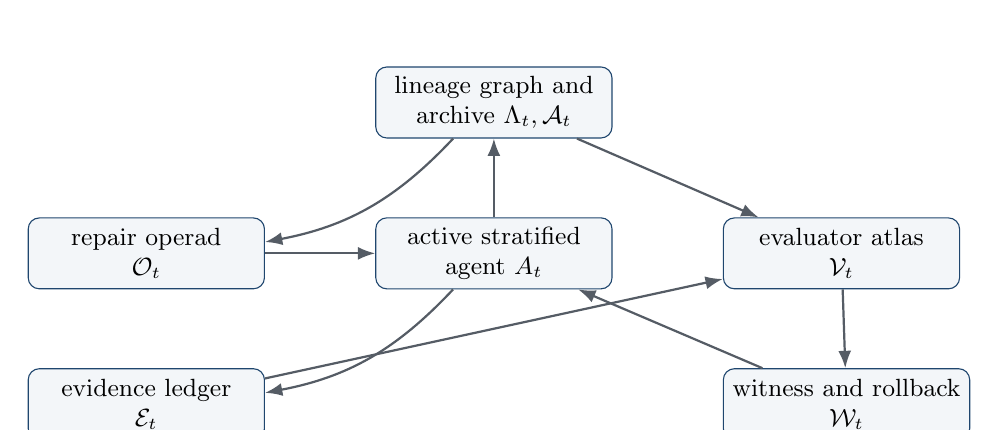
\begin{tikzpicture}[
  node distance=10mm and 14mm,
  box/.style={draw=KMBlue, rounded corners, fill=KMLight, align=center, minimum width=30mm, minimum height=9mm, font=\small},
  arr/.style={-{Latex[length=2.2mm]}, thick, draw=KMGray}
]
\node[box] (agent) {active stratified\\agent $A_t$};
\node[box, above=of agent] (lineage) {lineage graph and\\archive $\Lambda_t,\Acal_t$};
\node[box, left=of agent] (repair) {repair operad\\$\Ocal_t$};
\node[box, right=of agent] (eval) {evaluator atlas\\$\Vcal_t$};
\node[box, below left=of agent] (evidence) {evidence ledger\\$\Ecal_t$};
\node[box, below right=of agent] (witness) {witness and rollback\\$\Wcal_t$};
\draw[arr] (repair) -- (agent);
\draw[arr] (agent) -- (lineage);
\draw[arr] (lineage) -- (eval);
\draw[arr] (evidence) -- (eval);
\draw[arr] (eval) -- (witness);
\draw[arr] (witness) -- (agent);
\draw[arr, bend left=18] (agent) to (evidence);
\draw[arr, bend left=18] (lineage) to (repair);
\end{tikzpicture}
\caption{A resolved lineage state. No component alone is the persistent improving object; persistence is carried by their proof-carrying closure.}
\label{fig:resolved-lineage}
\end{figure}

\subsection{Lineage receipts and continuation}

\begin{definition}[Lineage-edge receipt]
A lineage edge
\begin{equation}
A\xrightarrow{\Pi}B
\end{equation}
has a receipt
\begin{equation}
\Pi=
\left(
\mathrm{id}_A,
\mathrm{id}_B,
\theta,
\Wcal,
\Ecal_{\mathrm{pre}},
\Ecal_{\mathrm{post}},
\widehat g,
\mathscr I,
\mathrm{tests},
\mathrm{decision},
\mathrm{rollback},
\mathrm{digest}
\right),
\end{equation}
recording the parent and child, transformation $\theta$, frozen witness, pre- and post-reveal evidence, precommitted effect claim $\widehat g$, protected invariants, validation results, commit decision, rollback point, and integrity digest.
\end{definition}

\begin{definition}[Validated continuation]
A descendant $B$ is a validated continuation of $A$ when there exists a directed path in $\Lambda$ from $A$ to $B$ whose every edge receipt is valid under the witness active at that edge.
\end{definition}

Structural equivalence does not imply validated continuation. Two copies may contain identical weights, memory, workspace state, and planner while occupying distinct nodes of $\Lambda$ because their causal histories and authorization paths differ.

\begin{theorem}[Category of validated lineage paths]
\label{thm:lineage-category}
Assume valid edge receipts are closed under proof-path concatenation and contain identity receipts for zero-change transitions. Then lineage states are objects and validated receipt paths are morphisms of a category $\mathbf{Lin}$.
\end{theorem}

\begin{proof}
The identity morphism on $A$ is the empty path with the identity receipt. Composition is path concatenation with receipt composition. Concatenation is associative, and the empty path is a left and right unit. Closure of valid receipts under concatenation ensures the composite is again a morphism.
\end{proof}

\begin{remark}
If every bridge in a path is invertible and its inverse has a valid receipt, the corresponding subcategory is a groupoid. Ordinary improvement lineages need not be invertible because training, compression, and evidence revelation are generally irreversible.
\end{remark}

\subsection{Forks and symmetry}

A lineage may branch:
\begin{equation}
A\longrightarrow B_1,
\qquad
A\longrightarrow B_2.
\end{equation}
No definition of recursive improvement requires one child to be the unique continuation of the parent.

\begin{theorem}[Symmetric forks do not justify unique selection]
\label{thm:fork-symmetry}
Let $D$ be all data available to a selector after a two-child fork. Suppose an involution $\sigma$ swaps $B_1$ and $B_2$ while leaving the witness, evidence, utilities, resource records, and lineage proofs invariant. Let a selector return a subset
\begin{equation}
s(D)\subseteq\{B_1,B_2\}
\end{equation}
and satisfy equivariance $s(\sigma D)=\sigma s(D)$. Then $s(D)$ cannot contain exactly one child.
\end{theorem}

\begin{proof}
Because $\sigma D=D$, equivariance gives $s(D)=\sigma s(D)$. The only subsets of $\{B_1,B_2\}$ fixed by the swap are $\varnothing$ and $\{B_1,B_2\}$. A singleton is not invariant.
\end{proof}

The result is operational rather than metaphysical. It says that a unique choice requires an asymmetry in evidence, resource allocation, policy, or tie-breaking rule. The archive may preserve both branches while a separate scheduler chooses which one receives the next experiment.

\subsection{Resolution consistency}

A lineage state is \emph{resolution-consistent} when:
\begin{enumerate}
\item every active component belongs to a declared stratum;
\item every cross-stratum inference cites a typed bridge and preservation profile;
\item every mutable belief used by the planner carries a provenance pointer into $\Ecal_t$ or is explicitly typed as simulation or hypothesis;
\item every repair operation belongs to $\Ocal_t$ or is quarantined as an untyped proposal;
\item every committed descendant has a valid receipt and rollback point;
\item every archived best-score claim can be reconstructed from protected traces and the evaluator version that produced it.
\end{enumerate}
Resolution consistency does not guarantee correctness. It prevents silent type changes from masquerading as theorem transport or causal evidence.

\section{Relative Introspection}

\subsection{Intervention semantics}

A self-improver need not reconstruct every internal degree of freedom. It needs a self-model sufficient for the authorized modifications it is currently considering.

Let $\Dcal_t$ be an authorized modification family containing a no-op intervention $\delta_0$. For $\delta\in\Dcal_t$, let
\begin{equation}
K_{A_t}^{\delta}(\cdot)
=
P\left(Y\in\cdot\mid \operatorname{do}(\delta),A_t\right)
\end{equation}
be the protected external-outcome kernel. A compressed causal self-model $\phi_t(A_t)$ induces a predicted kernel
\begin{equation}
\widehat K_{\phi_t(A_t)}^{\delta}(\cdot).
\end{equation}
The model is evaluated on counterfactual consequences, not on its ability to reproduce hidden activations for their own sake.

\begin{definition}[$\eps$-intervention sufficiency]
The map $\phi_t$ is $\eps$-intervention-sufficient for $\Dcal_t$ when
\begin{equation}
\sup_{\delta\in\Dcal_t}
\TV\left(
K_{A_t}^{\delta},
\widehat K_{\phi_t(A_t)}^{\delta}
\right)
\leq\eps.
\end{equation}
\end{definition}

The definition is relative to the current intervention grammar. It does not imply that the self-model is globally sufficient for arbitrary source-code rewrites, unseen tools, new sensors, or future ontology extensions.

\subsection{Decision regret and ranking competence}

\begin{theorem}[Decision regret from relative introspection]
\label{thm:introspection-regret}
Let $u:Y\to[0,1]$ be a bounded utility. Define
\begin{equation}
V(\delta)=\mathbb E[u(Y)\mid A_t,\delta],
\qquad
\widehat V(\delta)=\mathbb E[u(Y)\mid \phi_t(A_t),\delta].
\end{equation}
If $\phi_t$ is $\eps$-intervention-sufficient, then
\begin{equation}
\sup_{\delta\in\Dcal_t}
\abs{V(\delta)-\widehat V(\delta)}\leq\eps.
\end{equation}
If
\begin{equation}
\delta^*\in\argmax_{\delta\in\Dcal_t}V(\delta),
\qquad
\widehat\delta\in\argmax_{\delta\in\Dcal_t}\widehat V(\delta),
\end{equation}
then
\begin{equation}
V(\delta^*)-V(\widehat\delta)\leq2\eps.
\end{equation}
\end{theorem}

\begin{proof}
For probability measures at total-variation distance at most $\eps$, expectations of functions taking values in $[0,1]$ differ by at most $\eps$. Hence $\abs{V(\delta)-\widehat V(\delta)}\leq\eps$ uniformly. Then
\begin{align}
V(\delta^*)-V(\widehat\delta)
&\leq
V(\delta^*)-\widehat V(\delta^*)
+\widehat V(\widehat\delta)-V(\widehat\delta)\\
&\leq2\eps,
\end{align}
where $\widehat V(\widehat\delta)\geq\widehat V(\delta^*)$ was used.
\end{proof}

\begin{corollary}[Margin-preserving ranking]
\label{cor:ranking-margin}
If
\begin{equation}
V(\delta_1)-V(\delta_2)>2\eps,
\end{equation}
then
\begin{equation}
\widehat V(\delta_1)>\widehat V(\delta_2).
\end{equation}
In particular, if the true best intervention is unique and its gap from every alternative exceeds $2\eps$, the self-model selects the true best intervention.
\end{corollary}

\begin{proof}
One has
\begin{equation}
\widehat V(\delta_1)-\widehat V(\delta_2)
\geq
V(\delta_1)-V(\delta_2)-2\eps>0.
\end{equation}
\end{proof}

\begin{proposition}[Safe commit against a no-op baseline]
\label{prop:safe-commit}
Assume the same uniform error bound and let $\delta_0$ be the no-op. If a candidate $\delta$ is committed only when
\begin{equation}
\widehat V(\delta)-\widehat V(\delta_0)>2\eps,
\end{equation}
then the true gain is positive:
\begin{equation}
V(\delta)-V(\delta_0)>0.
\end{equation}
\end{proposition}

\begin{proof}
The true gain is bounded below by
\begin{equation}
V(\delta)-V(\delta_0)
\geq
\widehat V(\delta)-\widehat V(\delta_0)-2\eps>0.
\end{equation}
\end{proof}

\begin{corollary}[Cost-sensitive regret]
Suppose, in addition, that normalized intervention cost $c(\delta)$ is predicted by $\widehat c(\delta)$ with uniform error at most $\eps_c$. For net utility
\begin{equation}
W(\delta)=V(\delta)-\lambda c(\delta),
\qquad
\widehat W(\delta)=\widehat V(\delta)-\lambda\widehat c(\delta),
\end{equation}
selection by $\widehat W$ has regret at most
\begin{equation}
2\left(\eps+\lambda\eps_c\right).
\end{equation}
\end{corollary}

\begin{proof}
The net-utility approximation error is at most $\eps+\lambda\eps_c$. Apply the proof of \cref{thm:introspection-regret} with this error bound.
\end{proof}

\begin{remark}
Low average prediction error does not imply good candidate ranking. Selection depends on errors relative to pairwise gain margins. A model can estimate the mean effect of interventions accurately while systematically misordering the candidates near the decision boundary.
\end{remark}

\subsection{Coverage, expansion, and misspecification}

Define the intervention-coverage error
\begin{equation}
\eps_{\Dcal}(\phi;A)
=
\sup_{\delta\in\Dcal}
\TV\left(K_A^\delta,\widehat K_{\phi(A)}^\delta\right).
\end{equation}

\begin{proposition}[Coverage monotonicity]
If $\Dcal\subseteq\Dcal'$, then
\begin{equation}
\eps_{\Dcal'}(\phi;A)
\geq
\eps_{\Dcal}(\phi;A).
\end{equation}
\end{proposition}

\begin{proof}
The supremum is taken over a larger set.
\end{proof}

Thus an introspection guarantee does not automatically survive grammar expansion. Adding a new tool, parameter family, memory operation, or evaluator-edit operation enlarges the intervention class and requires new validation.

\begin{definition}[Intervention-complete relative to a repair grammar]
Let $\Ocal$ be a repair grammar and let $\Dcal(\Ocal)$ be the interventions denoted by its executable operations. A self-model is intervention-complete at tolerance $\eps$ relative to $\Ocal$ when it is $\eps$-intervention-sufficient for $\Dcal(\Ocal)$.
\end{definition}

This is a relative completeness notion. It makes no claim about interventions that the current grammar cannot express.

\subsection{Identifiability and active probing}

Let $\Hcal$ be a finite set of causal hypotheses about the source of a defect, such as internal model change, world change, memory corruption, sensor corruption, another agent's intervention, evaluator change, or an unknown mechanism. Let $\Pcal_{\mathrm{probe}}$ be a permitted probe family. Under hypothesis $h$ and probe $p$, the protected observation kernel is $K_h^p$.

\begin{theorem}[Observational indistinguishability]
\label{thm:observational-indistinguishability}
If two hypotheses $h,h'\in\Hcal$ satisfy
\begin{equation}
K_h^p=K_{h'}^p
\qquad
\text{for every permitted probe }p\in\Pcal_{\mathrm{probe}},
\end{equation}
then no adaptive decision rule based only on permitted probe transcripts can distinguish $h$ from $h'$ with different transcript distributions.
\end{theorem}

\begin{proof}
Proceed by induction over probe rounds. Before the first probe the transcript distributions coincide. If they coincide through round $k$, an adaptive policy chooses the same distribution over the next probe under both hypotheses because it is a function of the transcript. Conditional on every selected probe, the next observation kernels are equal. Therefore the round-$k+1$ transcript distributions coincide. The conclusion holds for every finite stopping time and hence for every decision rule measurable with respect to the transcript.
\end{proof}

\begin{definition}[Deterministically separating probe family]
Suppose every $K_h^p$ is a point mass at an outcome $y(h,p)$. The family $\Pcal_{\mathrm{probe}}$ separates $\Hcal$ when for every $h\neq h'$ there exists $p\in\Pcal_{\mathrm{probe}}$ such that
\begin{equation}
y(h,p)\neq y(h',p).
\end{equation}
\end{definition}

\begin{theorem}[Finite active identification]
\label{thm:finite-active-identification}
Let $\Hcal$ be finite and let $\Pcal_{\mathrm{probe}}$ be deterministically separating. Then an adaptive elimination procedure identifies the true hypothesis after at most $\abs{\Hcal}-1$ probes.
\end{theorem}

\begin{proof}
Maintain the set $S$ of hypotheses consistent with the transcript. If $\abs S>1$, choose distinct $h,h'\in S$ and a probe separating them. The observed outcome eliminates at least one of $h,h'$, so the size of $S$ decreases by at least one. Starting from $\abs{\Hcal}$ candidates, at most $\abs{\Hcal}-1$ reductions are required.
\end{proof}

\begin{remark}
No corresponding finite exact-identification guarantee follows automatically in the stochastic case. One instead needs quantitative separation, repeated evidence, posterior calibration, and an abstention rule when permitted evidence cannot resolve the hypotheses.
\end{remark}

\subsection{Prospective causal closure}

A useful self-model participates in a complete causal cycle:
\begin{equation}
\phi_t(A_t)
\xrightarrow{\text{candidate policy}}
\delta_t
\xrightarrow{\text{world execution}}
Y_{t+1}
\xrightarrow{\text{evidence update}}
\phi_{t+1}(A_{t+1}).
\end{equation}
The candidate is selected before the protected outcome is revealed. The outcome affects future beliefs and repair policy. Cutting either planner use or consequence feedback destroys prospective closure even if the internal self-representation remains decodable.

\begin{definition}[Prospectively closed self-model]
A self-model process is prospectively closed relative to $\Dcal$ when:
\begin{enumerate}
\item its state causally affects selection among interventions in $\Dcal$;
\item it predicts protected consequences before reveal;
\item committed outcomes update the future self-model and candidate policy;
\item the update distinguishes direct observation, communication, simulation, and imported memory by provenance type.
\end{enumerate}
\end{definition}

\subsection{Self-confirmation failure}

\begin{example}[Internal error reduction without external improvement]
Let the environment always produce protected outcome $Y=1$, independently of the agent's action. Let an internal predictor be $p\in\R$ with internal score
\begin{equation}
J_{\mathrm{int}}(p)=-(p-Y)^2.
\end{equation}
A self-intervention setting $p\leftarrow1$ improves $J_{\mathrm{int}}$ to zero error but does not change the world, task success, or action consequence. More extremely, an intervention that rewrites the error register itself can report zero error without even improving prediction. Therefore reduction of an endogenous mismatch is not external evidence of improvement unless the mismatch is tied to protected outcomes through a frozen causal test.
\end{example}

The example is intentionally elementary. Its role is to separate self-consistency from world-grounded competence. Relative introspection must be evaluated through consequences outside the mutable representation being improved.

\section{Proof-Carrying Repair Operads}

\subsection{From repair libraries to typed grammars}

A list of successful patches is not yet a repair calculus. A reusable repair mechanism must specify the systems to which a patch applies, the defect it is intended to alter, the evidence supporting that claim, the protected structures it may touch, the effects it predicts, and the rules by which it composes with other repairs.

Let $\mathsf C$ be the color set of the functional atlas. The syntactic repair grammar is a colored symmetric operad $\overline\Ocal$ with operation sets
\begin{equation}
\overline\Ocal(c_1,\ldots,c_n;c).
\end{equation}
An operation consumes typed inputs from strata $c_1,\ldots,c_n$ and produces a candidate correction in output stratum $c$.

\begin{definition}[Proof-carrying repair schema]
A repair schema is a tuple
\begin{equation}
\omega=
\left(
\sigma,
\bm c_{\mathrm{in}},
 c_{\mathrm{out}},
D,
C,
Q,
[r],
u,
\bm g,
\mathscr I,
\Pi
\right),
\end{equation}
where:
\begin{itemize}
\item $\sigma$ is a recognizable failure signature;
\item $\bm c_{\mathrm{in}}=(c_1,\ldots,c_n)$ and $c_{\mathrm{out}}$ are input and output colors;
\item $D$ is the declared local defect-response map;
\item $C$ is an applicability precondition;
\item $Q$ is a postcondition;
\item $[r]$ is a local obstruction certificate or unresolved-obstruction record;
\item $\nu$ is the correction program;
\item $\bm g$ is a precommitted effect profile;
\item $\mathscr I$ is a protected-invariant contract;
\item $\Pi$ is a proof, evidence, provenance, and rollback receipt.
\end{itemize}
\end{definition}

A useful effect profile is vector-valued:
\begin{equation}
\bm g=
\left(
\Delta J,
\Delta C,
\Delta R,
\eps_{\mathrm{leak}},
\eps_{\mathrm{hol}},
\Delta\Gamma,
\sigma_g
\right),
\end{equation}
recording predicted task gain, resource change, risk change, leakage, semantic holonomy, metaproductivity change, and uncertainty. Scalarizing this vector is an evaluator decision, not part of the repair syntax.

\subsection{Syntactic composition and semantic authorization}

Strictly speaking, applicability-dependent repair composition is partial. We therefore separate a total syntactic operad from an evidence-dependent authorization layer.

\begin{definition}[Proof-carrying repair operad]
A proof-carrying repair operad is a pair
\begin{equation}
\Ocal=(\overline\Ocal,\Valid),
\end{equation}
where $\overline\Ocal$ is a colored symmetric operad of syntactically composable repair programs and
\begin{equation}
\Valid_{\Ecal,\Wcal}(\omega,\Pi)
\in
\{\mathrm{valid},\mathrm{invalid},\mathrm{unresolved}\}
\end{equation}
is an evidence- and witness-indexed validation judgment. Only operations judged valid are executable. Unresolved operations remain quarantined.
\end{definition}

Each executable operation has a Hoare-style contract
\begin{equation}
\{C_\omega\}\ \omega\ \{Q_\omega\}.
\end{equation}
Syntactic substitution
\begin{equation}
\omega\circ(\omega_1,\ldots,\omega_n)
\end{equation}
is semantically authorized only when the inner postconditions and bridge guarantees imply the outer precondition.

\begin{definition}[Receipt composition]
Let $\Pi_i$ validate $\omega_i$, and let $\Pi$ validate the outer operation $\omega$ conditional on $C_\omega$. The composed receipt
\begin{equation}
\Pi\star(\Pi_1,\ldots,\Pi_n)
\end{equation}
is the provenance-directed acyclic graph obtained by proof-path concatenation, evidence union, explicit dependency links, and deduplication of immutable evidence references without duplicating linear observation authority.
\end{definition}

\begin{theorem}[Compositional receipt soundness]
\label{thm:receipt-soundness}
Assume:
\begin{enumerate}
\item every primitive receipt is semantically sound;
\item execution of each $\omega_i$ from $C_{\omega_i}$ establishes $Q_{\omega_i}$;
\item the conjunction of the inner postconditions and bridge guarantees implies $C_\omega$;
\item execution of $\omega$ from $C_\omega$ establishes $Q_\omega$;
\item receipt composition preserves provenance and protected evidence references.
\end{enumerate}
Then the composed receipt is sound for
\begin{equation}
\omega\circ(\omega_1,\ldots,\omega_n)
\end{equation}
with precondition $\bigwedge_iC_{\omega_i}$ and postcondition $Q_\omega$.
\end{theorem}

\begin{proof}
Starting from $\bigwedge_iC_{\omega_i}$, soundness of the primitive receipts and their operational contracts yields every $Q_{\omega_i}$. By assumption, these postconditions and the bridge guarantees establish $C_\omega$. Soundness of the outer receipt then yields $Q_\omega$. Because the composed receipt records the dependency graph and does not create new observation authority, the proof path certifies exactly this semantic composition.
\end{proof}

\begin{remark}
The theorem is conditional on a sound receipt checker and sound primitive contracts. It does not make an unverified learned claim true by placing it inside a receipt. The receipt exposes the claim, evidence, dependencies, and authority under which the claim may be used.
\end{remark}

\subsection{Sequential and parallel repair}

Sequential repair is operadic substitution. Parallel repair requires an additional compatibility test because two locally valid corrections may interfere through shared state or noncommuting updates.

Let $U$ and $V$ be bounded linear correction operators. Applying the updates in opposite orders gives
\begin{equation}
(I+U)(I+V)
\qquad\text{and}\qquad
(I+V)(I+U).
\end{equation}

\begin{proposition}[Exact order defect]
\label{prop:repair-order-defect}
The difference between the two update orders is the commutator:
\begin{equation}
(I+U)(I+V)-(I+V)(I+U)
=
[U,V]:=UV-VU.
\end{equation}
Hence the operator-norm order defect is exactly $\norm{[U,V]}$.
\end{proposition}

\begin{proof}
Expand both products and cancel $I$, $U$, and $V$.
\end{proof}

\begin{proposition}[Orthogonal packet repairs commute]
\label{prop:orthogonal-repairs}
Let $P$ and $Q$ be orthogonal projectors with $PQ=QP=0$. If
\begin{equation}
U=PUP,
\qquad
V=QVQ,
\end{equation}
then
\begin{equation}
UV=VU=0.
\end{equation}
Consequently the repairs commute exactly and
\begin{equation}
(I+U)(I+V)=I+U+V.
\end{equation}
\end{proposition}

\begin{proof}
One has
\begin{equation}
UV=PUPQVQ=0,
\qquad
VU=QVQPUP=0.
\end{equation}
\end{proof}

When support is only approximate, the commutator, cross-packet transfer energy, and protected-packet leakage become part of the composite effect profile. A parallel composition is authorized only when these quantities remain below declared tolerances.

\subsection{Conservative extensions}

\begin{definition}[Conservative repair-operad extension]
An inclusion
\begin{equation}
\iota_t:\Ocal_t\hookrightarrow\Ocal_{t+1}
\end{equation}
is conservative when:
\begin{enumerate}
\item it is injective on old colors and operations;
\item it preserves identities, permutations, and every old syntactic composition;
\item it preserves old preconditions, postconditions, and protected-invariant contracts on old states;
\item every previously valid old receipt remains valid against the same immutable evidence;
\item new operations cannot retroactively consume or rewrite old observation authority.
\end{enumerate}
\end{definition}

\begin{proposition}[Old derivations survive conservative extension]
Every valid repair expression and receipt derivation in $\Ocal_t$ remains valid after embedding into $\Ocal_{t+1}$.
\end{proposition}

\begin{proof}
This is immediate from preservation of operations, composition, contracts, validation judgments, and immutable evidence references.
\end{proof}

A nonconservative extension may still be scientifically justified, but it must be represented as a revision with explicit refutation or reinterpretation receipts rather than as silent monotone growth.

\subsection{Repair abstraction and generality}

A repair episode contains a concrete system state, defect, candidate correction, outcome, and receipt. Recursive compounding requires abstraction from episodes to reusable schemas.

\begin{definition}[Repair episode]
A repair episode is a tuple
\begin{equation}
e=
\left(
A,
r,
u,
Y_{\mathrm{pre}},
Y_{\mathrm{post}},
\Pi,
\bm g
\right).
\end{equation}
\end{definition}

\begin{definition}[Repair abstraction operator]
A repair abstraction operator is a map
\begin{equation}
\mathfrak a:
\mathcal H_{\mathrm{episodes}}
\longrightarrow
\overline\Ocal
\end{equation}
that maps one or more concrete episodes to a typed schema with a failure signature, applicability condition, correction program, effect profile, and receipt template.
\end{definition}

\begin{definition}[Schema generality preorder]
For repair schemas $\omega_1$ and $\omega_2$ with the same typed effect, write
\begin{equation}
\omega_1\preceq\omega_2
\end{equation}
when every state satisfying $C_{\omega_1}$ also satisfies $C_{\omega_2}$ and the two correction semantics agree on $\dom(C_{\omega_1})$ up to the declared transport tolerance. Then $\omega_2$ is at least as general as $\omega_1$.
\end{definition}

A schema is not validated as general merely because it compresses its training episodes. Its applicability condition and gain claim must be tested on foreign agents, new seeds, new task instances, or transformed representations not used to construct the abstraction.

\begin{definition}[Foreign-valid repair schema]
A repair schema is foreign-valid at margin $\gamma$ on a target distribution $\mathcal D$ when, under matched resources and its declared applicability predicate, the lower confidence bound on target gain is at least $\gamma$ and all protected invariants pass on agents sampled from $\mathcal D$ that are not descendants used to construct the schema.
\end{definition}

\subsection{Repair equivalence under exact transport}

Let $\omega_A$ and $\omega_B$ be repair schemas in systems $A$ and $B$. Suppose invertible maps transport their correction, defect, evidence, and stratum spaces.

\begin{definition}[Exact transport equivalence of repairs]
Write
\begin{equation}
\omega_A\cong_T\omega_B
\end{equation}
when:
\begin{enumerate}
\item input and output colors correspond under the atlas transport;
\item the defect-response maps commute with correction and defect transports;
\item applicability and postconditions are preserved in both directions;
\item protected invariants and provenance types are preserved;
\item the effect profiles agree after coordinate transport;
\item the receipts map to equivalent proof paths.
\end{enumerate}
\end{definition}

\begin{proposition}[Exact repair transports form a groupoid]
\label{prop:repair-groupoid}
Repair schemas as objects and exact invertible transport equivalences as morphisms form a groupoid.
\end{proposition}

\begin{proof}
The identity transport satisfies every condition. The inverse of an exact invertible transport preserves the commuting diagrams and receipt equivalence in the reverse direction. Composition of exact transports preserves types, commuting diagrams, contracts, invariants, effect profiles, and proof-path equivalence by ordinary composition. Hence every morphism is invertible.
\end{proof}

The approximate case is developed in \cref{sec:repair-transport}. There, transport equivalence is replaced by quantitative residual and gain bounds.

\subsection{Meta-repair}

\begin{definition}[Meta-repair]
A meta-repair is an authorized transformation
\begin{equation}
\Theta_t:\Ocal_t\longrightarrow\Ocal_{t+1}
\end{equation}
that changes one or more of:
\begin{enumerate}
\item failure-signature recognition;
\item causal-hypothesis generation;
\item candidate proposal distributions;
\item repair composition and scheduling;
\item receipt validation or confidence allocation;
\item repair abstraction and foreign-transfer testing.
\end{enumerate}
\end{definition}

A meta-repair is a genuine meta-improvement only if it improves held-out repair performance under matched resources. Adding a task-specific patch to the library may improve the current agent without improving the repair process itself.

\subsection{Example: a typed verification repair}

Consider four colors
\begin{equation}
\mathrm{memory},
\mathrm{representation},
\mathrm{verifier},
\mathrm{planner}.
\end{equation}
A composite factuality repair may have the form
\begin{equation}
\omega_{\mathrm{gate}}
\circ
\left(
\omega_{\mathrm{retrieve}},
\omega_{\mathrm{decompose}},
\omega_{\mathrm{check}}
\right).
\end{equation}
The inner operations retrieve evidence, decompose output into claims, and check claims against protected sources. Their postconditions establish the precondition for a planner gate that blocks or revises unsupported claims. The composite receipt records source provenance, claim-to-evidence links, verifier uncertainty, revised spans, latency cost, and regression results. If retrieval and checking use correlated or circular evidence, the outer precondition fails and the composite remains unresolved rather than being treated as verified merely because every module produced an output.

\section{Authorized Correction Geometry and Obstruction Calculus}
\label{sec:correctability}

\begin{statusbox}{Block 2 scope}
This block studies whether a declared defect is correctable by the currently authorized repair grammar. It separates five cases: exact linear correctability, quantitative least-squares repair, obstruction induced by protected invariants or one-sided authorization constraints, nonlinear obstruction beyond the first derivative, and cross-stratum incompatibility among otherwise valid local repairs.
\end{statusbox}

\subsection{Linear correction and quotient obstruction}

Let $U^{\Auth}$ and $V$ be finite-dimensional real Hilbert spaces. The first is the space of currently authorized infinitesimal corrections; the second is the space in which protected defects are measured. Let
\begin{equation}
D:U^{\Auth}\to V
\end{equation}
be the linearized defect-response map at the current lineage state. For a defect $r\in V$, an exact first-order repair satisfies
\begin{equation}
Du=-r.
\label{eq:linear-repair}
\end{equation}

\begin{definition}[Authorized obstruction class]
The authorized obstruction to correcting $r$ is
\begin{equation}
\Ob_D(r)=[r]\in\coker D:=V/\im D.
\end{equation}
\end{definition}

\begin{proposition}[Linear correctability]
Equation \eqref{eq:linear-repair} has an authorized solution if and only if
\begin{equation}
[r]=0\quad\text{in }\coker D.
\end{equation}
\end{proposition}

\begin{proof}
The equation is solvable exactly when $r\in\im D$, which is equivalent to vanishing of the quotient class.
\end{proof}

Binary solvability is insufficient for an engineering theory. A lineage must also know how far the defect lies from the correction range, which repair has minimum cost, and which component of the defect certifies failure.

\subsection{Canonical correctable and obstructed components}

Let $D^\dagger:V\to U^{\Auth}$ denote the Moore--Penrose pseudoinverse. Define
\begin{equation}
P_{\mathrm{cor}}:=DD^\dagger,
\qquad
P_{\mathrm{ob}}:=I_V-DD^\dagger.
\end{equation}

\begin{theorem}[Canonical correction--obstruction decomposition]
\label{thm:canonical-obstruction}
For every $r\in V$:
\begin{enumerate}
\item $P_{\mathrm{cor}}$ is the orthogonal projector onto $\im D$;
\item $P_{\mathrm{ob}}$ is the orthogonal projector onto $\ker D^*$;
\item the defect decomposes uniquely as
\begin{equation}
r=r_{\mathrm{cor}}+r_{\mathrm{ob}},
\qquad
r_{\mathrm{cor}}=P_{\mathrm{cor}}r,
\quad
r_{\mathrm{ob}}=P_{\mathrm{ob}}r;
\end{equation}
\item the minimum achievable residual is
\begin{equation}
\inf_{u\in U^{\Auth}}\norm{Du+r}
=\norm{r_{\mathrm{ob}}}
=\dist(r,\im D);
\end{equation}
\item the complete set of least-squares minimizers is
\begin{equation}
-D^\dagger r+\ker D;
\end{equation}
\item if $r$ is exactly correctable, $u^*=-D^\dagger r$ is the unique exact repair of minimum norm.
\end{enumerate}
\end{theorem}

\begin{proof}
The Moore--Penrose identities imply that $DD^\dagger$ is the orthogonal projector onto $\im D$ and that $I-DD^\dagger$ projects onto $(\im D)^\perp=\ker D^*$. For $u^*=-D^\dagger r$,
\begin{equation}
Du^*+r=(I-DD^\dagger)r=r_{\mathrm{ob}}.
\end{equation}
Every vector $Du$ lies in $\im D$, so orthogonal projection gives
\begin{equation}
\norm{Du+r}^2
=\norm{Du+r_{\mathrm{cor}}}^2+\norm{r_{\mathrm{ob}}}^2
\geq\norm{r_{\mathrm{ob}}}^2.
\end{equation}
Equality holds exactly when $Du=-r_{\mathrm{cor}}$, whose solution set is $-D^\dagger r+\ker D$. The Moore--Penrose solution is orthogonal to $\ker D$, hence has minimum norm.
\end{proof}

\begin{definition}[Quantitative authorized obstruction]
The quantitative obstruction magnitude is
\begin{equation}
\eta_D(r):=\norm{P_{\mathrm{ob}}r}=\dist(r,\im D).
\end{equation}
The normalized obstruction fraction is
\begin{equation}
\widehat\eta_D(r):=
\begin{cases}
\eta_D(r)/\norm r,&r\neq0,\\
0,&r=0.
\end{cases}
\end{equation}
\end{definition}

The quotient class $[r]$ records the exact algebraic obstruction. The scalar $\eta_D(r)$ records its metric severity. The two should not be conflated: a nonzero obstruction may be arbitrarily small, while a large correctable defect may have zero obstruction.

\begin{proposition}[Dual obstruction witness]
\label{prop:dual-obstruction}
For every $r\in V$,
\begin{equation}
\eta_D(r)
=
\max_{\substack{y\in\ker D^*\\ \norm y\leq1}}
\angles{y,r}.
\end{equation}
If $r_{\mathrm{ob}}\neq0$, the maximum is attained by
\begin{equation}
y^*=\frac{r_{\mathrm{ob}}}{\norm{r_{\mathrm{ob}}}}.
\end{equation}
\end{proposition}

\begin{proof}
For $y\in\ker D^*$, orthogonality gives $\angles{y,r}=\angles{y,r_{\mathrm{ob}}}$. Cauchy--Schwarz bounds this by $\norm{r_{\mathrm{ob}}}$, with equality at the displayed unit vector.
\end{proof}

The vector $y^*$ is a compact certificate: every authorized linear correction is invisible to it, yet the defect has nonzero projection along it.

\subsection{Protected invariants and resource-aware correction}

A repair is not authorized merely because it reduces task error. It must preserve declared invariants. Let
\begin{equation}
C:U\to Z
\end{equation}
be the derivative of a protected invariant map. First-order invariant preservation requires $Cu=0$, so the authorized tangent space is
\begin{equation}
U^{\Auth}=\ker C.
\end{equation}

\begin{proposition}[Invariant-constrained obstruction]
\label{prop:invariant-obstruction}
Let $D_C:=\restr{D}{\ker C}$. An exact first-order repair preserving the invariant exists if and only if
\begin{equation}
[r]=0\quad\text{in }\coker D_C.
\end{equation}
Equivalently, the stacked system
\begin{equation}
\begin{bmatrix}D\\C\end{bmatrix}u
=
\begin{bmatrix}-r\\0\end{bmatrix}
\end{equation}
is solvable.
\end{proposition}

\begin{proof}
The first statement is linear correctability on the restricted domain. The second rewrites the repair and invariant equations as one system.
\end{proof}

Thus a defect may be unconstrained-correctable but authorized-obstructed. This is the correct classification when a score can be improved only by deleting evidence, weakening provenance, exceeding an effect capability, or violating a protected safety or resource invariant.

Let $W:V\to V$ and $R:U\to U$ be positive-definite self-adjoint operators representing defect importance and repair cost.

\begin{theorem}[Regularized minimum-cost repair]
\label{thm:regularized-repair}
For $\lambda>0$, the functional
\begin{equation}
\Jcal_\lambda(u)
:=
\frac12\angles{Du+r,W(Du+r)}
+
\frac\lambda2\angles{u,Ru}
\end{equation}
has a unique minimizer
\begin{equation}
u_\lambda
=-(D^*WD+\lambda R)^{-1}D^*Wr.
\end{equation}
It is characterized by the normal equation
\begin{equation}
D^*W(Du_\lambda+r)+\lambda Ru_\lambda=0.
\end{equation}
\end{theorem}

\begin{proof}
The Hessian $D^*WD+\lambda R$ is positive definite because $R$ is positive definite and $\lambda>0$. Hence $\Jcal_\lambda$ is strictly convex and coercive. Differentiation gives the normal equation and its unique solution.
\end{proof}

Here $\lambda$ is not a semantic permission to trade away hard invariants. It balances only those costs already declared soft. Hard invariants remain in the domain restriction.

\subsection{Convex and one-sided authorization}

Some repairs are not closed under negation. Examples include adding tests, allocating nonnegative compute, increasing redundancy, or modifying parameters subject to inequality constraints. Let $K\subseteq U$ be a nonempty closed convex authorization set and define
\begin{equation}
\eta_{D,K}(r):=\inf_{u\in K}\norm{Du+r}.
\end{equation}

\begin{proposition}[Convex authorized correctability]
If $K$ is compact, or if $u\mapsto\norm{Du+r}$ is coercive on $K$, then the infimum defining $\eta_{D,K}(r)$ is attained. Exact authorized correction exists if and only if
\begin{equation}
\eta_{D,K}(r)=0.
\end{equation}
\end{proposition}

\begin{proof}
Continuity plus compactness gives attainment in the first case. Coercivity restricts every minimizing sequence to a compact sublevel set in finite dimension, giving the second. Exact correction is precisely zero residual.
\end{proof}

When $K$ is a cone, noncorrectability admits a Farkas-type dual witness. Define the dual cone
\begin{equation}
K^*:=\set{z\in U:\angles{z,u}\geq0\text{ for all }u\in K}.
\end{equation}

\begin{theorem}[Cone-constrained obstruction certificate]
\label{thm:cone-certificate}
Let $K\subseteq U$ be a closed convex cone and assume $D(K)$ is closed. Then an authorized correction $u\in K$ with $Du=-r$ exists if and only if
\begin{equation}
\angles{y,r}\leq0
\end{equation}
for every $y\in V$ satisfying
\begin{equation}
D^*y\in K^*.
\end{equation}
Consequently, any $y$ with $D^*y\in K^*$ and $\angles{y,r}>0$ certifies noncorrectability.
\end{theorem}

\begin{proof}
Set $C=D(K)$, a closed convex cone. Its dual is
\begin{equation}
C^*=\set{y:D^*y\in K^*}.
\end{equation}
By the bipolar theorem, $-r\in C$ if and only if $\angles{y,-r}\geq0$ for every $y\in C^*$, which is the displayed inequality.
\end{proof}

\subsection{Sensitivity, conditioning, and empirical certificates}

Let $\sigma_+(D)$ denote the smallest positive singular value of $D$. When $D\neq0$,
\begin{equation}
\norm{D^\dagger}=\frac{1}{\sigma_+(D)}.
\end{equation}
Small $\sigma_+(D)$ means the correctable component is ill-conditioned: a small defect perturbation may require a large repair.

\begin{proposition}[Fixed-map sensitivity]
For defects $r,s\in V$,
\begin{align}
\abs{\eta_D(r)-\eta_D(s)}&\leq\norm{r-s},\\
\norm{D^\dagger r-D^\dagger s}&\leq\frac{1}{\sigma_+(D)}\norm{r-s}.
\end{align}
\end{proposition}

\begin{proof}
The first inequality follows because distance to a fixed closed set is $1$-Lipschitz. The second follows from the operator norm of $D^\dagger$.
\end{proof}

\begin{proposition}[Transferred residual under model error]
\label{prop:correction-perturbation}
Let $\widehat D=D+\Delta D$ and $\widehat r=r+\Delta r$. For any proposed repair $u$,
\begin{equation}
\abs{\norm{Du+r}-\norm{\widehat Du+\widehat r}}
\leq
\norm{\Delta D}\norm u+\norm{\Delta r}.
\end{equation}
In particular, applying an exact repair for $(D,r)$ to the perturbed system yields residual at most
\begin{equation}
\norm{\Delta D}\norm u+\norm{\Delta r}.
\end{equation}
\end{proposition}

\begin{proof}
The two residual vectors differ by $\Delta D\,u+\Delta r$. Apply the reverse triangle inequality and submultiplicativity.
\end{proof}

The next result turns uncertain estimates into a budget-bounded obstruction certificate.

\begin{theorem}[Robust empirical noncorrectability certificate]
\label{thm:robust-obstruction-certificate}
Suppose, on an event of probability at least $1-\alpha$,
\begin{equation}
\norm{D-\widehat D}\leq\eps_D,
\qquad
\norm{r-\widehat r}\leq\eps_r.
\end{equation}
Fix a repair budget $\norm u\leq B$ and a unit vector $y\in V$. If
\begin{equation}
\angles{y,\widehat r}
>
\eps_r+B\bigl(\norm{\widehat D^*y}+\eps_D\bigr),
\label{eq:robust-dual-gap}
\end{equation}
then, on the same event, no budget-feasible repair satisfies $Du=-r$.
\end{theorem}

\begin{proof}
For every $\norm u\leq B$,
\begin{align}
\angles{y,Du+r}
&=\angles{D^*y,u}+\angles{y,r}\\
&\geq
-\norm{D^*y}\,B+\angles{y,\widehat r}-\eps_r\\
&\geq
-B\bigl(\norm{\widehat D^*y}+\eps_D\bigr)
+\angles{y,\widehat r}-\eps_r.
\end{align}
Condition \eqref{eq:robust-dual-gap} makes the final expression positive, so $Du+r$ cannot vanish.
\end{proof}

A negative result can therefore be proof-carrying: it records the witness $y$, the confidence event, the budget $B$, and the positive dual gap.

\subsection{Obstruction shrinkage under repair expansion}

Let $V$ remain fixed while the authorized correction grammar expands.

\begin{theorem}[Authorized obstruction-shrinkage theorem]
\label{thm:obstruction-shrinkage}
Suppose
\begin{equation}
U_t^{\Auth}\subseteq U_{t+1}^{\Auth}
\end{equation}
and
\begin{equation}
\restr{D_{t+1}}{U_t^{\Auth}}=D_t.
\end{equation}
Then
\begin{equation}
\im D_t\subseteq\im D_{t+1},
\end{equation}
there is a canonical surjection
\begin{equation}
q_t:\coker D_t\twoheadrightarrow\coker D_{t+1},
\qquad
[v]_{\im D_t}\longmapsto[v]_{\im D_{t+1}},
\end{equation}
and
\begin{equation}
\dim\coker D_{t+1}\leq\dim\coker D_t.
\end{equation}
The inequality is strict if and only if $\im D_t\subsetneq\im D_{t+1}$.
\end{theorem}

\begin{proof}
For $u\in U_t^{\Auth}$, $D_tu=D_{t+1}u$, so every old correctable direction remains correctable. Quotienting by a larger subspace gives the canonical surjection. Rank-nullity gives the dimension statement.
\end{proof}

\begin{definition}[Authorized repair rank]
The authorized repair rank and unresolved obstruction dimension are
\begin{equation}
\rho_t:=\rank D_t,
\qquad
o_t:=\dim\coker D_t.
\end{equation}
\end{definition}

\begin{proposition}[Exact sequence of newly correctable directions]
\label{prop:obstruction-exact-sequence}
Under the assumptions of \cref{thm:obstruction-shrinkage}, there is a short exact sequence
\begin{equation}
0
\longrightarrow
\frac{\im D_{t+1}}{\im D_t}
\longrightarrow
\coker D_t
\overset{q_t}{\longrightarrow}
\coker D_{t+1}
\longrightarrow0.
\end{equation}
Consequently,
\begin{equation}
o_t-o_{t+1}
=
\dim\frac{\im D_{t+1}}{\im D_t}.
\end{equation}
\end{proposition}

\begin{proof}
The kernel of $q_t$ consists exactly of classes represented by vectors in $\im D_{t+1}$, modulo $\im D_t$. Surjectivity was proved above. The dimension identity follows from exactness.
\end{proof}

The quotient $\im D_{t+1}/\im D_t$ is the marginal structural contribution of the new repair grammar. It counts newly reachable defect directions, not merely new source-code branches.

\subsection{Changing defect spaces}

Open-set improvement may enlarge the defect ontology itself. Let
\begin{equation}
j_U:U_t^{\Auth}\hookrightarrow U_{t+1}^{\Auth},
\qquad
j_V:V_t\hookrightarrow V_{t+1}
\end{equation}
be injective embeddings satisfying
\begin{equation}
D_{t+1}j_U=j_VD_t.
\label{eq:dynamic-defect-commute}
\end{equation}

\begin{proposition}[Induced obstruction transport under ontology expansion]
Equation \eqref{eq:dynamic-defect-commute} induces a linear map
\begin{equation}
\overline j_t:\coker D_t\to\coker D_{t+1},
\qquad
[v]\longmapsto[j_Vv].
\end{equation}
Its kernel is canonically isomorphic to
\begin{equation}
\ker\overline j_t
\cong
\frac{j_V(V_t)\cap\im D_{t+1}}{j_V(\im D_t)}.
\end{equation}
Thus an old obstruction vanishes after expansion exactly when the enlarged repair grammar corrects its embedded defect direction.
\end{proposition}

\begin{proof}
Commutation ensures that changing the representative by $D_tu$ changes $j_Vv$ by $D_{t+1}j_Uu$, so the map is well-defined. The formula for the kernel follows directly from the quotient definition.
\end{proof}

An evidence-conservative ontology expansion should make $j_V$ explicit. Otherwise disappearance of an old defect may reflect semantic deletion rather than newly acquired correctability.

\subsection{Packet-resolved correction and cross-packet leakage}

Let
\begin{equation}
U=\bigoplus_{i=1}^m U_i,
\qquad
V=\bigoplus_{i=1}^m V_i,
\end{equation}
with orthogonal projectors $Q_i$ and $P_i$. Decompose
\begin{equation}
D=D_0+E,
\qquad
D_0:=\sum_{i=1}^m P_iDQ_i.
\end{equation}
The block-diagonal operator $D_0$ represents ideal packet-local correction; $E$ contains all cross-packet effects.

Suppose each local block admits a right inverse and their direct sum gives
\begin{equation}
Q_0:V\to U,
\qquad
D_0Q_0=I_V.
\end{equation}

\begin{theorem}[Exact correction under small packet coupling]
\label{thm:packet-neumann}
If
\begin{equation}
q:=\norm{EQ_0}<1,
\end{equation}
then $D$ is surjective and has right inverse
\begin{equation}
Q
=Q_0(I_V+EQ_0)^{-1}
=Q_0\sum_{k=0}^{\infty}(-EQ_0)^k.
\end{equation}
Moreover,
\begin{equation}
\norm Q\leq\frac{\norm{Q_0}}{1-q}.
\end{equation}
For defect $r$, the truncated packet-correction series
\begin{equation}
u^{(n)}
:=-Q_0\sum_{k=0}^{n}(-EQ_0)^kr
\end{equation}
has residual
\begin{equation}
Du^{(n)}+r=(-EQ_0)^{n+1}r,
\end{equation}
and hence
\begin{equation}
\norm{Du^{(n)}+r}\leq q^{n+1}\norm r.
\end{equation}
\end{theorem}

\begin{proof}
Since $\norm{EQ_0}<1$, the Neumann series for $(I+EQ_0)^{-1}$ converges. Also
\begin{equation}
DQ_0=(D_0+E)Q_0=I+EQ_0,
\end{equation}
so $DQ=I$. The norm bound follows from the geometric series. For the truncation,
\begin{equation}
(I+EQ_0)\sum_{k=0}^n(-EQ_0)^k
=I-(-EQ_0)^{n+1},
\end{equation}
which gives the residual formula.
\end{proof}

This theorem formalizes a useful middle regime. Cross-packet effects need not vanish. They must be sufficiently small relative to the local correction inverse for iterative coordination to converge.

\begin{definition}[Packet leakage profile]
The directed leakage from correction packet $j$ into defect packet $i$ is
\begin{equation}
\ell_{ij}:=\norm{P_iDQ_j},
\qquad i\neq j.
\end{equation}
The matrix $(\ell_{ij})$ is the packet leakage profile.
\end{definition}

A repair receipt should record both the target block and this off-block profile. A patch that corrects its intended packet while strongly disturbing protected packets is not locally authorized merely because the total score improves.

\subsection{Gauge-fixed nonlinear local repair by contraction}

Let $U,V$ be Banach spaces and let the post-correction defect map be
\begin{equation}
\Fcal(u)=r+Du+N(u),
\qquad N(0)=0.
\end{equation}
When $D$ has a nontrivial kernel, a bounded right inverse does not make the full nonlinear repair unique: two roots can differ along neutral or symmetry directions. The contraction argument therefore requires a declared complement, or gauge, in which the right inverse selects one representative.

\begin{theorem}[Gauge-fixed local nonlinear repair by contraction]
\label{thm:nonlinear-repair}
Suppose $D:U\to V$ has a bounded right inverse $Q:V\to U$, so $DQ=I_V$, and set
\begin{equation}
W:=\im Q.
\end{equation}
Then $\restr D W:W\to V$ is an isomorphism with inverse $Q$. Let
\begin{equation}
B_R^W:=\set{w\in W:\norm w\leq R}.
\end{equation}
Suppose
\begin{equation}
\norm{N(u)-N(v)}\leq L_N\norm{u-v}
\qquad(u,v\in B_R^W),
\end{equation}
with
\begin{equation}
q:=\norm QL_N<1,
\end{equation}
and
\begin{equation}
\norm{Qr}+\norm Q\sup_{u\in B_R^W}\norm{N(u)}\leq R.
\end{equation}
Then there exists a unique $u^*\in B_R^W$ satisfying $\Fcal(u^*)=0$. The gauge-fixed iteration
\begin{equation}
u_{k+1}=-Qr-QN(u_k)
\end{equation}
converges to $u^*$ from every $u_0\in B_R^W$, with
\begin{equation}
\norm{u_k-u^*}\leq\frac{q^k}{1-q}\norm{u_1-u_0}.
\end{equation}
\end{theorem}

\begin{proof}
Define $T(u)=-Qr-QN(u)$. Because $T$ takes values in $W$, the radius condition gives $T(B_R^W)\subseteq B_R^W$. The Lipschitz condition gives
\begin{equation}
\norm{T(u)-T(v)}\leq q\norm{u-v}.
\end{equation}
Banach's fixed-point theorem yields a unique fixed point in $B_R^W$ and the standard a posteriori convergence estimate. Applying $D$ to the fixed-point equation and using $DQ=I_V$ gives $Du^*=-r-N(u^*)$.
\end{proof}

\begin{remark}[Scope of uniqueness]
The theorem proves uniqueness only in the selected gauge $W=\im Q$. Other roots may exist elsewhere in $U$ when $\ker D\neq0$. Such roots must be compared through the later Lyapunov--Schmidt reduction, cost criteria, or explicit symmetry quotients rather than being ruled out by the contraction argument.
\end{remark}

\begin{proposition}[Nonlinear obstruction floor]
\label{prop:nonlinear-floor}
Let $P_{\mathrm{ob}}$ be the orthogonal obstruction projector of $D$. For every $u$,
\begin{equation}
\norm{\Fcal(u)}
\geq
\norm{P_{\mathrm{ob}}r}-\norm{P_{\mathrm{ob}}N(u)}.
\end{equation}
Consequently, if $\norm{P_{\mathrm{ob}}N(u)}\leq\gamma$ on an authorized region, then no repair in that region can achieve residual below
\begin{equation}
\max\set{0,\eta_D(r)-\gamma}.
\end{equation}
\end{proposition}

\begin{proof}
Since $P_{\mathrm{ob}}D=0$,
\begin{equation}
P_{\mathrm{ob}}\Fcal(u)=P_{\mathrm{ob}}r+P_{\mathrm{ob}}N(u).
\end{equation}
Apply the reverse triangle inequality and $\norm{\Fcal(u)}\geq\norm{P_{\mathrm{ob}}\Fcal(u)}$.
\end{proof}

A first-order obstruction can sometimes be canceled by nonlinear terms. The proposition quantifies how large that nonlinear obstruction-channel effect must be.

\subsection{Newton--Kantorovich repair}

The gauge-fixed contraction theorem assumes a fixed linear right inverse and a selected complement. Newton iteration permits a changing derivative.

\begin{theorem}[Newton--Kantorovich repair criterion]
\label{thm:newton-kantorovich}
Let $F:U\to V$ be continuously Fr\'echet differentiable between Banach spaces. Let $u_0\in U$ and suppose $F'(u_0)$ is invertible with inverse $B$. Assume that on the closed ball $\overline B(u_0,R)$,
\begin{equation}
\norm{F'(u)-F'(v)}\leq L\norm{u-v}.
\end{equation}
Set
\begin{equation}
\eta:=\norm{BF(u_0)},
\qquad
h:=\norm B\,L\eta.
\end{equation}
If $h\leq\frac12$ and
\begin{equation}
t_*:=\frac{1-\sqrt{1-2h}}{\norm B\,L}\leq R,
\end{equation}
then Newton iteration
\begin{equation}
u_{n+1}=u_n-F'(u_n)^{-1}F(u_n)
\end{equation}
is well-defined, remains in $\overline B(u_0,t_*)$, and converges to a root $u^*$ of $F$. If the larger radius
\begin{equation}
t^{**}:=\frac{1+\sqrt{1-2h}}{\norm B\,L}
\end{equation}
is contained in the regularity region, the root is unique in $\overline B(u_0,t^{**})$.
\end{theorem}

\begin{proof}
Consider the scalar majorant
\begin{equation}
f(t)=\eta-t+\frac{\norm B\,L}{2}t^2.
\end{equation}
The condition $h\leq1/2$ gives the two nonnegative roots $t_*$ and $t^{**}$. The Lipschitz derivative bound and the Banach lemma imply that $F'(u)$ remains invertible while $\norm{u-u_0}<1/(\norm B L)$. Standard Newton majorization shows that the increments of the operator iteration are dominated by those of scalar Newton iteration for $f$, whose partial sums remain below $t_*$ and converge. Hence $(u_n)$ is Cauchy, its limit lies in the ball, and continuity gives $F(u^*)=0$. The same majorant estimate gives uniqueness in the larger ball.
\end{proof}

The criterion makes three quantities auditable: the initial predicted correction size $\eta$, inverse sensitivity $\norm B$, and derivative curvature $L$.

\subsection{Singular nonlinear repair and Lyapunov--Schmidt reduction}

When $D=F'(0)$ is not surjective, the nonlinear problem is not decided by a global right inverse. The correct local object is a reduced obstruction equation.

\begin{theorem}[Lyapunov--Schmidt repair reduction]
\label{thm:lyapunov-schmidt}
Let $F:P\times U\to V$ be $C^k$, $k\geq2$, between finite-dimensional spaces, with $F(0,0)=0$. Let
\begin{equation}
D:=\partial_uF(0,0).
\end{equation}
Choose splittings
\begin{equation}
U=K\oplus X,
\qquad
K=\ker D,
\end{equation}
and
\begin{equation}
V=R\oplus C,
\qquad
R=\im D,
\end{equation}
so that $\restr{D}{X}:X\to R$ is an isomorphism. Let $P_R$ and $P_C$ be the corresponding projections. Then there are neighborhoods of the origin and a unique $C^k$ map
\begin{equation}
\chi:P\times K\to X,
\qquad
\chi(0,0)=0,
\end{equation}
such that
\begin{equation}
P_RF(p,k+\chi(p,k))=0.
\end{equation}
Define the reduced obstruction map
\begin{equation}
\psi(p,k):=P_CF(p,k+\chi(p,k)).
\end{equation}
A sufficiently small pair $(p,u)$ solves $F(p,u)=0$ if and only if
\begin{equation}
u=k+\chi(p,k)
\end{equation}
for some $k\in K$ satisfying
\begin{equation}
\psi(p,k)=0.
\end{equation}
\end{theorem}

\begin{proof}
Apply the implicit-function theorem to the range equation
\begin{equation}
G(p,k,x):=P_RF(p,k+x)=0.
\end{equation}
Its derivative in $x$ at the origin is $\restr D X:X\to R$, an isomorphism, so there is a unique local solution $x=\chi(p,k)$. Substitution solves the range component identically. The remaining equation is exactly the cokernel component $\psi(p,k)=0$.
\end{proof}

The reduction shows why ``vanishing linear obstruction'' is not the end of the analysis. Kernel freedom $k$ may be used to solve the reduced cokernel equation, may produce several branches, or may fail completely.

\subsection{Higher-order obstruction classes}

Consider the specific formal correction equation
\begin{equation}
F(\eps,u)
=
\eps r_1+Du+\frac12B(u,u)+O\bigl(\eps^3+\norm u^3\bigr),
\label{eq:second-order-model}
\end{equation}
where $B:U\times U\to V$ is symmetric bilinear. Seek
\begin{equation}
u(\eps)=\eps u_1+\eps^2u_2+O(\eps^3).
\end{equation}

\begin{proposition}[Second-order repair obstruction]
\label{prop:second-order-obstruction}
A repair through order $\eps^2$ exists only if
\begin{align}
Du_1&=-r_1,\\
\left[\frac12B(u_1,u_1)\right]&=0
\quad\text{in }\coker D.
\end{align}
When the second class vanishes, $u_2$ may be chosen to solve
\begin{equation}
Du_2=-\frac12B(u_1,u_1).
\end{equation}
If $\ker D\neq0$, replacing $u_1$ by $u_1+k$ can change the second-order obstruction class.
\end{proposition}

\begin{proof}
Substitute the formal series into \eqref{eq:second-order-model} and equate coefficients of $\eps$ and $\eps^2$. The first equation is the linear repair equation. The second is solvable exactly when its right-hand side has zero class in $\coker D$.
\end{proof}

\begin{theorem}[Finite formal obstruction tower]
\label{thm:formal-obstruction-tower}
Let $F(\eps,u)$ be analytic near $(0,0)$ with $F(0,0)=0$ and $D=\partial_uF(0,0)$. Suppose coefficients $u_1,\ldots,u_{n-1}$ have been chosen so that
\begin{equation}
F\left(\eps,\sum_{j=1}^{n-1}\eps^ju_j\right)
=\eps^nb_n+O(\eps^{n+1}).
\end{equation}
Then extending the repair to order $n$ by adding $\eps^nu_n$ is possible if and only if
\begin{equation}
[b_n]=0\quad\text{in }\coker D.
\end{equation}
When it vanishes, any solution of $Du_n=-b_n$ produces an order-$n$ lift.
\end{theorem}

\begin{proof}
Analytic expansion gives
\begin{equation}
F\left(\eps,\sum_{j=1}^{n}\eps^ju_j\right)
=
\eps^n(b_n+Du_n)+O(\eps^{n+1}),
\end{equation}
because $u_n$ first enters linearly at order $n$. Cancellation of the coefficient is equivalent to solvability of $Du_n=-b_n$.
\end{proof}

The sequence
\begin{equation}
[b_1],[b_2],[b_3],\ldots\in\coker D
\end{equation}
is an obstruction tower. Choices in $\ker D$ at early orders can alter later classes, so a repair search must retain branch information rather than greedily fixing one representative.

\section{Local-to-Global Repair Descent}
\label{sec:repair-descent}

\subsection{Repair sheaves and local solution torsors}

A heterogeneous agent may admit valid repairs in every stratum while those repairs remain mutually incompatible. Let $X$ be a finite site of functional regions and let
\begin{equation}
\mathfrak U=\set{U_\alpha}_{\alpha\in I}
\end{equation}
be a finite cover. Let $\mathscr U$ be a sheaf of authorized corrections, $\mathscr V$ a sheaf of defects, and
\begin{equation}
D:\mathscr U\to\mathscr V
\end{equation}
a morphism of sheaves. Let $r\in\Gamma(X,\mathscr V)$ be a global defect.

A local correction on $U_\alpha$ is a section $u_\alpha\in\mathscr U(U_\alpha)$ satisfying
\begin{equation}
D_\alpha u_\alpha=-r|_{U_\alpha}.
\end{equation}
If one local correction exists, the local solution set is an affine space over $\ker D(U_\alpha)$.

\begin{proposition}[Local solution torsor]
For each $U_\alpha$, the set
\begin{equation}
\Sscr_\alpha
:=
\set{u\in\mathscr U(U_\alpha):D_\alpha u=-r|_{U_\alpha}}
\end{equation}
is either empty or a torsor for the additive group $\ker D(U_\alpha)$. If a global repair exists, the global solution set is a torsor for $\Gamma(X,\ker D)$.
\end{proposition}

\begin{proof}
The difference of two solutions lies in the kernel, and adding a kernel section to a solution preserves the equation. The action is free and transitive.
\end{proof}

This torsor viewpoint matters because a local repair is rarely unique. Kernel freedom is the resource used to reconcile interface assumptions.

\subsection{Exact linear descent}

\begin{theorem}[Linear repair-descent theorem]
\label{thm:repair-descent}
Assume a local correction $u_\alpha$ exists on every $U_\alpha$. On overlaps $U_{\alpha\beta}=U_\alpha\cap U_\beta$, define
\begin{equation}
d_{\alpha\beta}
:=
\restr{u_\alpha}{U_{\alpha\beta}}
-
\restr{u_\beta}{U_{\alpha\beta}}.
\end{equation}
Then:
\begin{enumerate}
\item $d_{\alpha\beta}\in\ker D(U_{\alpha\beta})$;
\item $(d_{\alpha\beta})$ is a \v{C}ech $1$-cocycle with coefficients in $\ker D$;
\item a global correction $u\in\Gamma(X,\mathscr U)$ with $Du=-r$ exists if and only if $(d_{\alpha\beta})$ is a \v{C}ech coboundary relative to $\mathfrak U$.
\end{enumerate}
If the cover computes first cohomology, the final condition is equivalent to
\begin{equation}
[d_{\alpha\beta}]=0
\quad\text{in}\quad
\check H^1(X,\ker D).
\end{equation}
\end{theorem}

\begin{proof}
On every overlap,
\begin{equation}
D(d_{\alpha\beta})
=-r|_{U_{\alpha\beta}}+r|_{U_{\alpha\beta}}=0.
\end{equation}
On triple overlaps,
\begin{equation}
d_{\alpha\beta}+d_{\beta\gamma}+d_{\gamma\alpha}=0,
\end{equation}
so the family is a cocycle.

If a global repair $u$ exists, set $k_\alpha=u|_{U_\alpha}-u_\alpha$. Then $Dk_\alpha=0$ and
\begin{equation}
d_{\alpha\beta}=k_\beta-k_\alpha,
\end{equation}
so the cocycle is a coboundary. Conversely, if $d_{\alpha\beta}=k_\beta-k_\alpha$ for kernel sections $k_\alpha$, then $u'_\alpha=u_\alpha+k_\alpha$ agree on overlaps. The sheaf gluing axiom yields a global $u$, and $Du=-r$ because the adjustments lie in the kernel.
\end{proof}

\begin{definition}[Two-level repair obstruction]
The local obstruction on $U_\alpha$ is
\begin{equation}
[r|_{U_\alpha}]\in\coker D_\alpha.
\end{equation}
When every local class vanishes, the global gluing obstruction is
\begin{equation}
[d_{\alpha\beta}]\in\check H^1(\mathfrak U,\ker D).
\end{equation}
\end{definition}

\begin{proposition}[Choice independence of the gluing class]
The cohomology class $[d_{\alpha\beta}]$ does not depend on the particular family of local repairs used to compute it.
\end{proposition}

\begin{proof}
If $u'_\alpha=u_\alpha+k_\alpha$ with $k_\alpha\in\ker D(U_\alpha)$, then
\begin{equation}
d'_{\alpha\beta}
=d_{\alpha\beta}+k_\alpha-k_\beta.
\end{equation}
Thus the cocycles differ by a coboundary.
\end{proof}

Repair failure now has two distinct meanings:
\begin{enumerate}
\item a chart cannot correct its own defect;
\item every chart can correct locally, but the chosen repairs cannot be made globally coherent.
\end{enumerate}

\subsection{Graph-Hodge decomposition of approximate gluing}

The exact \v{C}ech class is binary. Empirical repairs produce noisy overlap mismatches. A finite graph model gives a quantitative analogue.

Let $G=(I,E)$ be a connected oriented graph representing the nerve of the cover, let $K$ be a finite-dimensional Hilbert space representing a common trivialization of the kernel fibers, and let
\begin{equation}
e=(e_a)_{a\in E}\in K^E
\end{equation}
be the transported overlap-mismatch vector. Let $B\in\R^{|I|\times|E|}$ be the oriented incidence matrix and set
\begin{equation}
\mathbf B:=B\otimes I_K.
\end{equation}
A vertex gauge $k\in K^I$ changes the mismatch to
\begin{equation}
e+\mathbf B^*k.
\end{equation}

\begin{theorem}[Quantitative graph-Hodge gluing]
\label{thm:graph-hodge-gluing}
Let
\begin{equation}
L_G:=BB^*
\end{equation}
be the graph Laplacian and let $P_{\mathrm{cyc}}$ be the orthogonal projector from $K^E$ onto
\begin{equation}
\ker\mathbf B,
\end{equation}
the cycle space. Then
\begin{equation}
\inf_{k\in K^I}\norm{e+\mathbf B^*k}
=
\norm{P_{\mathrm{cyc}}e}.
\end{equation}
The mean-zero minimum-norm gauge is
\begin{equation}
k^*
=-(L_G^\dagger B\otimes I_K)e.
\end{equation}
If $\lambda_2(L_G)>0$ is the spectral gap, then
\begin{equation}
\norm{k^*}
\leq
\frac{1}{\sqrt{\lambda_2(L_G)}}\norm e.
\end{equation}
Exact graph-level gluing is possible if and only if
\begin{equation}
P_{\mathrm{cyc}}e=0.
\end{equation}
\end{theorem}

\begin{proof}
The finite-dimensional Hodge decomposition is
\begin{equation}
K^E=\im\mathbf B^*\oplus\ker\mathbf B.
\end{equation}
A gauge can remove exactly the gradient component in $\im\mathbf B^*$, leaving the cycle projection. The normal equation for the least-squares gauge is
\begin{equation}
\mathbf B\mathbf B^*k=-\mathbf Be,
\end{equation}
whose mean-zero minimum-norm solution is the displayed pseudoinverse expression. The smallest nonzero singular value of $\mathbf B^*$ is $\sqrt{\lambda_2(L_G)}$, giving the bound.
\end{proof}

\begin{definition}[Quantitative gluing obstruction]
The graph-level quantitative gluing obstruction is
\begin{equation}
\eta_{\mathrm{glue}}(e)
:=\norm{P_{\mathrm{cyc}}e}.
\end{equation}
The local-to-global repair certificate is the pair
\begin{equation}
\left(
\eta_{\mathrm{loc}},
\eta_{\mathrm{glue}}
\right),
\qquad
\eta_{\mathrm{loc}}^2
:=\sum_{\alpha}\norm{D_\alpha u_\alpha+r_\alpha}^2.
\end{equation}
\end{definition}

A small local residual does not imply a small gluing residual. Conversely, a perfectly coherent family can consistently implement the wrong local repair. Both coordinates are required.

\begin{corollary}[Trees have no cycle obstruction]
If the cover nerve is a tree, then $\ker\mathbf B=0$ and every overlap mismatch can be removed by a vertex gauge. Any remaining failure is local rather than cyclic.
\end{corollary}

\begin{proof}
A connected tree has $|E|=|I|-1$ and incidence matrix of full column rank, so its cycle space is zero.
\end{proof}

\subsection{Weighted overlap confidence}

Different overlaps may have different uncertainty or semantic importance. Let $W_E$ be a positive-definite operator on $K^E$. Define
\begin{equation}
\eta_{\mathrm{glue},W}(e)
:=
\inf_k\norm{e+\mathbf B^*k}_{W_E}.
\end{equation}

\begin{proposition}[Weighted gluing normal equation]
Every weighted least-squares gauge satisfies
\begin{equation}
\mathbf BW_E\mathbf B^*k
=-\mathbf BW_Ee.
\end{equation}
The mean-zero minimum-norm minimizer is
\begin{equation}
k_W^*
=-\bigl(\mathbf BW_E\mathbf B^*\bigr)^\dagger\mathbf BW_Ee.
\end{equation}
The irreducible weighted mismatch is the $W_E$-orthogonal projection of $e$ onto the $W_E$-orthogonal complement of $\im\mathbf B^*$.
\end{proposition}

\begin{proof}
Differentiate the quadratic objective
\begin{equation}
\frac12\angles{e+\mathbf B^*k,W_E(e+\mathbf B^*k)}
\end{equation}
with respect to $k$. The normal equation follows. Its Moore--Penrose solution is the unique minimizer orthogonal to the constant vertex-gauge kernel.
\end{proof}

This permits confidence-weighted descent: weakly identified interfaces need not dominate a certificate merely because they have large raw coordinate scale.

\subsection{Finite cycle obstruction}

\begin{example}[Locally repairable, globally incompatible]
Let the nerve be a three-cycle with no triple intersection. Suppose the kernel fiber is $\R$ and the oriented differences are
\begin{equation}
d_{12}=1,
\qquad
d_{23}=1,
\qquad
d_{31}=1.
\end{equation}
If the cocycle were a coboundary, there would be $k_1,k_2,k_3$ with
\begin{equation}
d_{12}=k_2-k_1,
\quad
d_{23}=k_3-k_2,
\quad
d_{31}=k_1-k_3.
\end{equation}
Summing gives $3=0$, a contradiction. Hence no global correction exists. The graph-Hodge obstruction has norm $\sqrt3$.
\end{example}

In an agent, the three charts might represent planner, memory, and evaluator repairs. Each patch can pass isolated tests while the cycle of interface assumptions fails to close.

\subsection{Nonlinear descent through symmetry torsors}

For nonlinear repair, local solution sets need not be affine. A tractable case occurs when each local solution set is a principal homogeneous space for a local symmetry group.

Let $\mathscr G$ be a sheaf of groups acting freely and transitively on the sheaf of local nonlinear solutions $\mathscr S$. Choose local solutions $s_\alpha\in\mathscr S(U_\alpha)$. On overlaps there are unique transition elements
\begin{equation}
g_{\alpha\beta}\in\mathscr G(U_{\alpha\beta})
\end{equation}
such that
\begin{equation}
s_\alpha=g_{\alpha\beta}\cdot s_\beta.
\end{equation}

\begin{conditionaltheorem}[Nonlinear torsor descent]
\label{thm:nonlinear-torsor-descent}
Assume the local solution action is principal and effective descent holds for $\mathscr G$-torsors on the declared cover. Then a global nonlinear repair exists if and only if the transition family satisfies the nonabelian cocycle condition
\begin{equation}
g_{\alpha\beta}g_{\beta\gamma}g_{\gamma\alpha}=e
\end{equation}
on triple overlaps and its class is trivial in nonabelian \v{C}ech cohomology
\begin{equation}
[g_{\alpha\beta}]=1
\quad\text{in}\quad
\check H^1(\mathfrak U,\mathscr G).
\end{equation}
Equivalently, there exist local gauges $g_\alpha\in\mathscr G(U_\alpha)$ such that
\begin{equation}
g_{\alpha\beta}=g_\alpha^{-1}g_\beta.
\end{equation}
\end{conditionaltheorem}

\begin{proof}
If a global solution exists, compare its restriction with each $s_\alpha$ to obtain gauges $g_\alpha$; their ratios give the transition functions. Conversely, triviality of the cocycle permits gauge-adjusted local solutions $g_\alpha\cdot s_\alpha$ that agree on overlaps. Effective descent glues them to a global solution.
\end{proof}

The theorem is conditional because arbitrary nonlinear repair spaces need not be torsors, and arbitrary software interfaces need not satisfy effective descent.

\subsection{Spanning-tree holonomy test}

A finite operational version avoids explicit cohomology. Let $G=(I,E)$ be connected, with sets of local solutions $S_i$ and invertible transition maps
\begin{equation}
T_{ij}:S_i\to S_j,
\qquad
T_{ji}=T_{ij}^{-1}.
\end{equation}
Choose a root $o$ and a spanning tree $T\subseteq G$.

\begin{theorem}[Fundamental-cycle holonomy criterion]
\label{thm:fundamental-holonomy}
For each root state $s_o\in S_o$, tree transport determines a unique family $(s_i^T)$. For every non-tree edge $e=(i,j)$, let $H_e:S_o\to S_o$ be transport around the corresponding fundamental cycle. The tree family extends to a globally compatible family on all edges if and only if
\begin{equation}
H_e(s_o)=s_o
\end{equation}
for every non-tree edge $e$.
\end{theorem}

\begin{proof}
Tree edges are compatible by construction. A non-tree edge closes one fundamental cycle. Its compatibility is exactly the statement that transport from the root to $i$, across $e$, and back to the root returns $s_o$. Fundamental cycles generate all graph cycles, so satisfying every chord condition gives compatibility on all edges.
\end{proof}

\begin{definition}[Nonlinear holonomy residual]
If the $S_i$ are metric spaces, define
\begin{equation}
\eta_{\mathrm{hol}}(s_o)
:=
\max_{e\in E\setminus T}d\bigl(H_e(s_o),s_o\bigr).
\end{equation}
\end{definition}

This is a direct finite test for path dependence of repair semantics. It is distinct from the evaluator holonomy developed later, though mathematically analogous.

\subsection{Order-by-order global repair}

The local nonlinear tower and the descent obstruction combine into a two-axis lifting problem. Suppose each chart has an analytic local repair equation with the same linearized sheaf morphism $D$.

At order $n$, let
\begin{equation}
b_{n,\alpha}\in\mathscr V(U_\alpha)
\end{equation}
be the residual coefficient determined by lower-order choices. The local obstruction is
\begin{equation}
[b_{n,\alpha}]\in\coker D_\alpha.
\end{equation}
If every local class vanishes, choose $u_{n,\alpha}$ with
\begin{equation}
D_\alpha u_{n,\alpha}=-b_{n,\alpha}.
\end{equation}
Their differences define an order-$n$ gluing class in $\check H^1(\ker D)$.

\begin{theorem}[Finite local-to-global obstruction tower]
\label{thm:global-obstruction-tower}
Fix $N\in\N$. Assume:
\begin{enumerate}
\item the analytic local repair equations agree under restriction;
\item the sheaves $\mathscr U$ and $\mathscr V$ satisfy effective linear descent on the declared cover;
\item repairs have been constructed globally through order $n-1$.
\end{enumerate}
Then a global repair extends through order $n$ if and only if:
\begin{enumerate}
\item every local coefficient class vanishes,
\begin{equation}
[b_{n,\alpha}]=0\quad\text{in }\coker D_\alpha;
\end{equation}
\item for one, hence every, choice of local lifts, the overlap class vanishes,
\begin{equation}
[d^{(n)}_{\alpha\beta}]=0
\quad\text{in}\quad
\check H^1(\mathfrak U,\ker D).
\end{equation}
\end{enumerate}
If both conditions hold for every $1\leq n\leq N$, a global formal repair exists through order $N$.
\end{theorem}

\begin{proof}
At order $n$, coefficient matching reduces the local problem to the linear equation $D_\alpha u_{n,\alpha}=-b_{n,\alpha}$, so the local cokernel classes are the complete local obstruction. When they vanish, \cref{thm:repair-descent} gives the complete criterion for gluing the order-$n$ coefficients. Induction from $1$ through $N$ constructs the global formal series.
\end{proof}

The theorem produces an obstruction ledger
\begin{equation}
\begin{array}{c|cc}
\text{order}&\text{local obstruction}&\text{gluing obstruction}\\
\hline
1&[b_{1,\alpha}]\in\coker D_\alpha&[d^{(1)}]\in\check H^1(\ker D)\\
2&[b_{2,\alpha}]\in\coker D_\alpha&[d^{(2)}]\in\check H^1(\ker D)\\
\vdots&\vdots&\vdots\\
N&[b_{N,\alpha}]\in\coker D_\alpha&[d^{(N)}]\in\check H^1(\ker D).
\end{array}
\end{equation}
Higher categorical repair interfaces may introduce additional coherence obstructions beyond this two-column ledger. Those are not proved here.

\subsection{Cover refinement and diagnostic soundness}

\begin{proposition}[Soundness of cover-relative obstruction]
If a global repair exists, then every local obstruction and every exact gluing obstruction vanishes on every cover. Therefore, a nonzero local or gluing class on any valid cover is a sound certificate of global nonexistence.
\end{proposition}

\begin{proof}
Restrict the global repair to each chart. The local equations hold, and the local restrictions agree exactly on overlaps, producing zero cocycles.
\end{proof}

The converse depends on the sheaf and cover assumptions of \cref{thm:repair-descent}. A poor atlas can obscure causal structure even when its internal descent computation is correct. Atlas discovery therefore remains logically prior to universal claims about repair.

\begin{definition}[Cover adequacy score]
For a candidate functional cover $\mathfrak U$, define the diagnostic score
\begin{equation}
\Acal(\mathfrak U)
:=
\eta_{\mathrm{loc}}(\mathfrak U)
+\tau\eta_{\mathrm{glue}}(\mathfrak U)
+\lambda\,\mathrm{Complexity}(\mathfrak U)
+\gamma\,\mathrm{Instability}(\mathfrak U).
\end{equation}
\end{definition}

This is a model-selection objective, not a theorem that the minimizing cover is uniquely correct. Its purpose is to expose the tradeoff between local fit, global coherence, atlas complexity, and instability under resampling or intervention.

\section{Repair Transport and Transfer Geometry}\label{sec:repair-transport}

A repair discovered in one system becomes recursively useful only when the system can determine whether the repair remains meaningful after a change of architecture, representation, task coordinates, or evaluator. Transport is therefore not an auxiliary convenience. It is the mechanism by which a local correction becomes a reusable element of the repair calculus.

The theory separates four logically distinct questions:
\begin{enumerate}
\item does the correction equation commute with the proposed representation maps;
\item does the transport preserve authorization, invariants, and resource budgets;
\item how do transport errors accumulate along a path through an atlas;
\item does the transported correction retain positive externally measured gain?
\end{enumerate}
The answers need not coincide. A correction may commute algebraically while violating an authorization cone. It may remain authorized while losing gain under evaluator mismatch. It may work along one transport path and fail along another because of nontrivial holonomy.

\subsection{Correction data and transport morphisms}

\begin{definition}[Correction datum]
A finite-dimensional correction datum is a tuple
\begin{equation}
\mathfrak C=(U,V,D,\Acal,c,\mathfrak p),
\end{equation}
where $U$ is a correction space, $V$ is a defect space, $D:U\to V$ is the linearized defect-response map, $\Acal\subseteq U$ is the authorized correction set, $c:U\to[0,\infty]$ is a declared resource cost, and $\mathfrak p$ is a collection of protected predicates or invariant maps.
\end{definition}

\begin{definition}[Transport datum]
Let $\mathfrak C_A$ and $\mathfrak C_B$ be correction data. A transport datum from $A$ to $B$ is a pair
\begin{equation}
\mathfrak T_{A\to B}=(T_U,T_V),
\qquad
T_U:U_A\to U_B,
\qquad
T_V:V_A\to V_B.
\end{equation}
Its correction-square defect is
\begin{equation}
\Delta_D(\mathfrak T_{A\to B})
:=
D_BT_U-T_VD_A.
\end{equation}
For declared source and target defects $r_A\in V_A$ and $r_B\in V_B$, its defect-identification error is
\begin{equation}
\Delta_r(\mathfrak T_{A\to B};r_A,r_B)
:=
r_B-T_Vr_A.
\end{equation}
The datum is \emph{exact} when both quantities vanish.
\end{definition}

The two errors answer different questions. $\Delta_D$ measures failure of the correction mechanism to commute. $\Delta_r$ measures failure of the target defect to be the transported source defect. A small value of one does not imply a small value of the other.

\begin{theorem}[Exact repair transport]
\label{thm:exact-transport}
Suppose
\begin{equation}
D_BT_U=T_VD_A
\end{equation}
and
\begin{equation}
r_B=T_Vr_A.
\end{equation}
If $u_A$ satisfies
\begin{equation}
D_Au_A=-r_A,
\end{equation}
then
\begin{equation}
u_B:=T_Uu_A
\end{equation}
satisfies
\begin{equation}
D_Bu_B=-r_B.
\end{equation}
\end{theorem}

\begin{proof}
By commutation,
\begin{equation}
D_Bu_B=D_BT_Uu_A=T_VD_Au_A=-T_Vr_A=-r_B.
\end{equation}
\end{proof}

\begin{corollary}[Kernel and obstruction naturality]
\label{cor:kernel-coker-naturality}
Assume $D_BT_U=T_VD_A$. Then
\begin{equation}
T_U(\ker D_A)\subseteq\ker D_B
\end{equation}
and
\begin{equation}
T_V(\im D_A)\subseteq\im D_B.
\end{equation}
Consequently, $T_V$ induces a quotient map
\begin{equation}
\overline T_V:\coker D_A\to\coker D_B,
\qquad
[r]\mapsto[T_Vr].
\end{equation}
\end{corollary}

\begin{proof}
If $D_Au=0$, then $D_BT_Uu=T_VD_Au=0$. If $v=D_Au$, then $T_Vv=D_BT_Uu\in\im D_B$. The quotient map is therefore well-defined.
\end{proof}

\begin{theorem}[Exact transport equivalence]
\label{thm:transport-equivalence}
Suppose $T_U$ and $T_V$ are isomorphisms and
\begin{equation}
D_B=T_VD_AT_U^{-1}.
\end{equation}
Then $T_U$ restricts to an isomorphism
\begin{equation}
\ker D_A\cong\ker D_B,
\end{equation}
and $T_V$ induces an isomorphism
\begin{equation}
\coker D_A\cong\coker D_B.
\end{equation}
Thus exact transport equivalence preserves both correction freedom and obstruction dimension.
\end{theorem}

\begin{proof}
The kernel statement follows from \cref{cor:kernel-coker-naturality} applied in both directions. Since $T_U$ is surjective,
\begin{equation}
\im D_B
=
T_VD_AT_U^{-1}(U_B)
=
T_V(\im D_A).
\end{equation}
Hence $T_V$ maps $\im D_A$ bijectively onto $\im D_B$ and descends to an isomorphism of quotient spaces.
\end{proof}

\begin{definition}[Protected obstruction subspace]
A protected obstruction subspace is a declared subspace
\begin{equation}
Q_A\subseteq\coker D_A
\end{equation}
whose nonzero classes must remain detectable after transport. The transport is \emph{obstruction-faithful on $Q_A$} when
\begin{equation}
\ker\overline T_V\cap Q_A=\set{0}.
\end{equation}
\end{definition}

\begin{proposition}[Representation loss can hide an obstruction]
\label{prop:hidden-obstruction}
If $\overline T_V$ is not injective, then there exists a defect $r_A$ such that
\begin{equation}
[r_A]\neq0
\quad\text{but}\quad
[T_Vr_A]=0.
\end{equation}
Thus the target representation classifies the transported defect as correctable even though the source obstruction is nonzero. Obstruction faithfulness is therefore a necessary condition whenever the erased class is protected.
\end{proposition}

\begin{proof}
Choose a nonzero class in $\ker\overline T_V$ and any representative $r_A$. By definition its image in $\coker D_B$ vanishes.
\end{proof}

\begin{remark}
A noninjective bridge may be useful as a compression map, but it cannot by itself certify preservation of every repair obstruction. This is the transport analogue of the distinction between exact representation change and information-losing abstraction.
\end{remark}

\subsection{Authorization, invariants, and minimum-cost correction}

\begin{definition}[Authorized transport]
A transport datum is authorized when
\begin{equation}
T_U(\Acal_A)\subseteq\Acal_B.
\end{equation}
It is $(c_A,c_B,\kappa)$-budget controlled when
\begin{equation}
c_B(T_Uu)\leq\kappa c_A(u)
\qquad
\text{for every }u\in\Acal_A.
\end{equation}
\end{definition}

\begin{proposition}[Authorized exact repair transport]
\label{prop:authorized-transport}
Under the hypotheses of \cref{thm:exact-transport}, if $u_A\in\Acal_A$ and the transport is authorized, then $u_B=T_Uu_A$ is an authorized exact repair in system $B$. If, in addition, $c_A(u_A)\leq B$ and the transport is $(c_A,c_B,\kappa)$-budget controlled, then
\begin{equation}
c_B(u_B)\leq\kappa B.
\end{equation}
\end{proposition}

\begin{proof}
Authorization follows from $T_U(\Acal_A)\subseteq\Acal_B$. Exact repair follows from \cref{thm:exact-transport}. The cost inequality is the definition of budget control.
\end{proof}

Let protected linear invariants be represented by
\begin{equation}
C_A:U_A\to Z_A,
\qquad
C_B:U_B\to Z_B.
\end{equation}
A correction preserves the invariant when $C_Au=0$ or $C_Bu=0$.

\begin{proposition}[Invariant-preserving transport]
\label{prop:invariant-transport}
Suppose there is a linear map $S:Z_A\to Z_B$ satisfying
\begin{equation}
C_BT_U=SC_A.
\end{equation}
Then
\begin{equation}
T_U(\ker C_A)\subseteq\ker C_B.
\end{equation}
Consequently, every source repair preserving the declared invariant transports to a target repair preserving the transported invariant.
\end{proposition}

\begin{proof}
For $u\in\ker C_A$,
\begin{equation}
C_BT_Uu=SC_Au=0.
\end{equation}
\end{proof}

The previous propositions guarantee feasibility, not optimality. Under unitary transport, the canonical minimum-norm correction is also preserved.

\begin{theorem}[Naturality of the Moore--Penrose repair]
\label{thm:pseudoinverse-transport}
Let $U_A,U_B,V_A,V_B$ be finite-dimensional Hilbert spaces. Suppose $T_U$ and $T_V$ are unitary and
\begin{equation}
D_B=T_VD_AT_U^*.
\end{equation}
Then
\begin{equation}
D_B^{\dagger}=T_UD_A^{\dagger}T_V^*.
\end{equation}
For every $r_B=T_Vr_A$, the target minimum-norm least-squares correction is the transport of the source minimum-norm least-squares correction:
\begin{equation}
-D_B^{\dagger}r_B
=
T_U(-D_A^{\dagger}r_A).
\end{equation}
The orthogonal obstruction projectors satisfy
\begin{equation}
I-D_BD_B^{\dagger}
=
T_V(I-D_AD_A^{\dagger})T_V^*.
\end{equation}
\end{theorem}

\begin{proof}
Set $X=T_UD_A^{\dagger}T_V^*$. Direct substitution, unitary cancellation, and the four Moore--Penrose equations for $D_A^{\dagger}$ show that $X$ satisfies the four Moore--Penrose equations for $D_B$. Uniqueness gives $X=D_B^{\dagger}$. The correction and projector identities follow immediately.
\end{proof}

\begin{remark}
For nonunitary isomorphisms, exact repairability still transports, but minimum norm is coordinate dependent. A change of metric or an explicit condition-number penalty is then required before comparing repair costs.
\end{remark}

\subsection{Composition and accumulation of transport defect}

Let
\begin{equation}
\mathfrak T_{A\to B}=(T_U^{AB},T_V^{AB}),
\qquad
\mathfrak T_{B\to C}=(T_U^{BC},T_V^{BC}).
\end{equation}
The composed transport is
\begin{equation}
\mathfrak T_{A\to C}
=
(T_U^{BC}T_U^{AB},T_V^{BC}T_V^{AB}).
\end{equation}

\begin{lemma}[Composition identity]
\label{lem:transport-composition}
The correction-square defects obey
\begin{equation}
\Delta_D(\mathfrak T_{A\to C})
=
\Delta_D(\mathfrak T_{B\to C})T_U^{AB}
+
T_V^{BC}\Delta_D(\mathfrak T_{A\to B}).
\end{equation}
The defect-identification errors obey
\begin{equation}
\Delta_r(\mathfrak T_{A\to C})
=
\Delta_r(\mathfrak T_{B\to C})
+
T_V^{BC}\Delta_r(\mathfrak T_{A\to B}).
\end{equation}
\end{lemma}

\begin{proof}
Insert and subtract $T_V^{BC}D_BT_U^{AB}$ in the first expression and $T_V^{BC}r_B$ in the second.
\end{proof}

\begin{theorem}[Pathwise transport bound]
\label{thm:pathwise-transport}
Consider a path of systems
\begin{equation}
A_0\xrightarrow{\mathfrak T_0}A_1
\xrightarrow{\mathfrak T_1}\cdots
\xrightarrow{\mathfrak T_{n-1}}A_n.
\end{equation}
Write $T_{U,k}:U_k\to U_{k+1}$ and $T_{V,k}:V_k\to V_{k+1}$. Let
\begin{equation}
\norm{D_{k+1}T_{U,k}-T_{V,k}D_k}\leq\eps_{D,k}
\end{equation}
and
\begin{equation}
\norm{r_{k+1}-T_{V,k}r_k}\leq\eps_{r,k}.
\end{equation}
If $D_0u_0=-r_0$ and
\begin{equation}
u_n=T_{U,n-1}\cdots T_{U,0}u_0,
\end{equation}
then
\begin{equation}
\begin{aligned}
\norm{D_nu_n+r_n}
&\leq
\sum_{k=0}^{n-1}
\norm{T_{V,n-1}\cdots T_{V,k+1}}
\eps_{D,k}
\norm{T_{U,k-1}\cdots T_{U,0}u_0}\\
&\quad+
\sum_{k=0}^{n-1}
\norm{T_{V,n-1}\cdots T_{V,k+1}}
\eps_{r,k},
\end{aligned}
\end{equation}
where empty products are identities.
\end{theorem}

\begin{proof}
Repeatedly apply \cref{lem:transport-composition}. The total correction-square defect is the telescoping sum
\begin{equation}
\sum_{k=0}^{n-1}
T_{V,n-1}\cdots T_{V,k+1}
\Delta_{D,k}
T_{U,k-1}\cdots T_{U,0},
\end{equation}
and the total defect-identification error is
\begin{equation}
\sum_{k=0}^{n-1}
T_{V,n-1}\cdots T_{V,k+1}\Delta_{r,k}.
\end{equation}
Apply both sums to $u_0$, use $D_0u_0+r_0=0$, and take norms.
\end{proof}

\begin{corollary}[Nonexpansive path bound]
\label{cor:nonexpansive-path}
If every $T_{U,k}$ and $T_{V,k}$ is nonexpansive, then
\begin{equation}
\norm{D_nu_n+r_n}
\leq
\norm{u_0}\sum_{k=0}^{n-1}\eps_{D,k}
+
\sum_{k=0}^{n-1}\eps_{r,k}.
\end{equation}
\end{corollary}

\begin{definition}[Transport route cost]
For a fixed source correction $u_0$, define the certified cost of a nonexpansive path $p$ by
\begin{equation}
C_{\mathrm{tr}}(p;u_0)
:=
\norm{u_0}\sum_{e\in p}\eps_{D,e}
+
\sum_{e\in p}\eps_{r,e}
+
\sum_{e\in p}\eps_{\mathrm{auth},e}
+
\sum_{e\in p}\eps_{\mathrm{sem},e}.
\end{equation}
\end{definition}

\begin{proposition}[Shortest certified route]
\label{prop:shortest-route}
When all edge transports are nonexpansive and the declared error contributions are additive, a shortest path in the edge-weighted transport graph minimizes the stated worst-case transfer penalty and therefore maximizes the corresponding certified lower bound on target gain.
\end{proposition}

\begin{proof}
Under the hypotheses, the path penalty is the sum of nonnegative edge costs. Minimizing this sum is exactly the shortest-path problem.
\end{proof}

\begin{remark}
If some transports amplify norms, route quality depends on the prefix and suffix products in \cref{thm:pathwise-transport}; a scalar edge weight is no longer sufficient. The routing state must then retain the current transported correction norm and downstream amplification profile.
\end{remark}

\subsection{Repair holonomy and path dependence}

Let $G$ be a graph of correction data with invertible exact transports. For a loop $\gamma$ based at system $A$, define correction and defect holonomies
\begin{equation}
H^U_\gamma:U_A\to U_A,
\qquad
H^V_\gamma:V_A\to V_A.
\end{equation}
Exact commutation along the loop gives
\begin{equation}
D_AH^U_\gamma=H^V_\gamma D_A.
\end{equation}

\begin{definition}[Path-flat repair and defect cores]
The path-flat repair and defect cores at $A$ are
\begin{equation}
U_A^{\flat}
:=
\bigcap_\gamma\ker(H^U_\gamma-I),
\qquad
V_A^{\flat}
:=
\bigcap_\gamma\ker(H^V_\gamma-I).
\end{equation}
\end{definition}

\begin{proposition}[Flat repairs remain flat defects]
\label{prop:flat-repair-defect}
If $u\in U_A^{\flat}$, then
\begin{equation}
D_Au\in V_A^{\flat}.
\end{equation}
\end{proposition}

\begin{proof}
For every loop $\gamma$,
\begin{equation}
H^V_\gamma D_Au=D_AH^U_\gamma u=D_Au.
\end{equation}
\end{proof}

\begin{theorem}[Path independence on the flat repair core]
\label{thm:path-independence}
Let $p$ and $q$ be two exact invertible transport paths from $A$ to $B$. If $u\in U_A$ is fixed by the loop holonomy associated with $q^{-1}p$, then
\begin{equation}
T_U^p u=T_U^q u.
\end{equation}
In particular, every $u\in U_A^{\flat}$ has path-independent transport to $B$.
\end{theorem}

\begin{proof}
The path identity is
\begin{equation}
T_U^p=T_U^qH^U_{q^{-1}p}.
\end{equation}
Apply both sides to $u$ and use $H^U_{q^{-1}p}u=u$.
\end{proof}

\begin{definition}[Repair holonomy residual]
For a correction $u$ and loop $\gamma$, define
\begin{equation}
\eta^U_\gamma(u)
:=
\norm{(H^U_\gamma-I)u}.
\end{equation}
For a defect $r$, define
\begin{equation}
\eta^V_\gamma(r)
:=
\norm{(H^V_\gamma-I)r}.
\end{equation}
\end{definition}

\begin{proposition}[Path-discrepancy identity]
\label{prop:path-discrepancy}
Under the hypotheses of \cref{thm:path-independence},
\begin{equation}
\norm{T_U^pu-T_U^qu}
\leq
\norm{T_U^q}\,\eta^U_{q^{-1}p}(u).
\end{equation}
Thus loop holonomy directly bounds disagreement between two transport routes.
\end{proposition}

\begin{proof}
Use
\begin{equation}
T_U^pu-T_U^qu=T_U^q(H^U_{q^{-1}p}-I)u
\end{equation}
and take norms.
\end{proof}

\subsection{Approximate transported residual}

\begin{theorem}[Approximate transported residual]
\label{thm:approx-residual}
Let $U_A,U_B,V_A,V_B$ be normed spaces. Suppose $u_A$ solves
\begin{equation}
D_Au_A=-r_A.
\end{equation}
Assume
\begin{equation}
\norm{D_BT_U-T_VD_A}\leq\eps_D
\end{equation}
and
\begin{equation}
\norm{r_B-T_Vr_A}\leq\eps_r.
\end{equation}
Then $u_B=T_Uu_A$ satisfies
\begin{equation}
\norm{D_Bu_B+r_B}
\leq
\eps_D\norm{u_A}+\eps_r.
\end{equation}
\end{theorem}

\begin{proof}
Add and subtract $T_VD_Au_A$ and $T_Vr_A$:
\begin{align}
D_BT_Uu_A+r_B
&=
(D_BT_U-T_VD_A)u_A
+T_V(D_Au_A+r_A)
+(r_B-T_Vr_A).
\end{align}
The middle term vanishes. Taking norms yields the claim.
\end{proof}

\begin{definition}[Scale-normalized transport defect]
For a declared stabilizer $\tau>0$, define
\begin{equation}
\eps_D^{\mathrm{rel}}
:=
\frac{\norm{D_BT_U-T_VD_A}}
{\norm{D_B}\norm{T_U}+\norm{T_V}\norm{D_A}+\tau}.
\end{equation}
\end{definition}

The normalized defect is not a substitute for the absolute residual in \cref{thm:approx-residual}. It is a diagnostic for comparing transport squares at different numerical scales. Both quantities should be retained in a repair receipt.

\subsection{Deterministic gain preservation}

Let $\ell_A:V_A\to\R$ and $\ell_B:V_B\to\R$ be post-defect losses. Define source and target gains
\begin{equation}
g_A
:=
\ell_A(r_A)-\ell_A(r_A+D_Au_A),
\end{equation}
\begin{equation}
g_B
:=
\ell_B(r_B)-\ell_B(r_B+D_BT_Uu_A).
\end{equation}

\begin{assumption}[Evaluator alignment]
There is $\eps_J\geq0$ such that
\begin{equation}
\abs{\ell_B(T_Vv)-\ell_A(v)}\leq\eps_J
\end{equation}
for
\begin{equation}
v\in\set{r_A,r_A+D_Au_A}.
\end{equation}
\end{assumption}

\begin{theorem}[Approximate gain-preserving repair transport]
\label{thm:gain-transport}
Assume $\ell_B$ is $L$-Lipschitz. Suppose the hypotheses of \cref{thm:approx-residual} hold. Let additional target-side perturbations from packet leakage and semantic holonomy have total defect norm at most
\begin{equation}
\eps_{\mathrm{leak}}+\eps_{\mathrm{hol}}.
\end{equation}
Then
\begin{equation}
\boxed{
 g_B
\geq
 g_A
-2\eps_J
-L\left(
2\eps_r
+\eps_D\norm{u_A}
+\eps_{\mathrm{leak}}
+\eps_{\mathrm{hol}}
\right).
}
\end{equation}
In particular, the transported repair is guaranteed beneficial whenever the source gain exceeds the total right-hand error margin.
\end{theorem}

\begin{proof}
Evaluator alignment and Lipschitz continuity imply
\begin{equation}
\ell_B(r_B)
\geq
\ell_B(T_Vr_A)-L\eps_r
\geq
\ell_A(r_A)-\eps_J-L\eps_r.
\end{equation}
The target post-repair defect differs from
\begin{equation}
T_V(r_A+D_Au_A)
\end{equation}
by at most
\begin{equation}
\eps_r+\eps_D\norm{u_A}+\eps_{\mathrm{leak}}+\eps_{\mathrm{hol}}
\end{equation}
using \cref{thm:approx-residual} and the declared additional perturbation bounds. Hence
\begin{align}
\ell_B(r_B+D_BT_Uu_A)
&\leq
\ell_B(T_V(r_A+D_Au_A))\\
&\quad+L\left(
\eps_r+\eps_D\norm{u_A}
+\eps_{\mathrm{leak}}+\eps_{\mathrm{hol}}
\right)\\
&\leq
\ell_A(r_A+D_Au_A)+\eps_J\\
&\quad+L\left(
\eps_r+\eps_D\norm{u_A}
+\eps_{\mathrm{leak}}+\eps_{\mathrm{hol}}
\right).
\end{align}
Subtracting the post-repair upper bound from the baseline lower bound gives the result.
\end{proof}

\begin{corollary}[Pathwise gain certificate]
\label{cor:pathwise-gain}
Along a nonexpansive transport path, replace
\begin{equation}
\eps_D\norm{u_A}+\eps_r
\end{equation}
by the pathwise residual bound in \cref{cor:nonexpansive-path}. If the source gain exceeds twice the evaluator-alignment error plus the resulting Lipschitz, leakage, and holonomy penalties, then the endpoint repair retains positive certified gain.
\end{corollary}

\begin{remark}
The theorem makes repair transfer falsifiable. A failed transfer can be attributed to defect mismatch, correction noncommutation, evaluator mismatch, packet leakage, authorization loss, or semantic holonomy rather than being described only as distribution shift.
\end{remark}

\subsection{Distributional and probabilistic transfer certificates}

The deterministic theorem compares declared defects. A deployed repair is usually evaluated across a distribution of contexts. Let $P_A$ and $P_B$ be source and target context distributions, let $S:X_A\to X_B$ be a declared context transport, and let $q_A,q_B$ be per-context repair gains.

\begin{theorem}[Coupled distributional gain transfer]
\label{thm:distributional-transfer}
Suppose there is a coupling $\pi$ of $P_A$ and $P_B$ such that
\begin{equation}
\mathbb E_{(x,y)\sim\pi}d_B(y,Sx)\leq\delta.
\end{equation}
Assume $q_B$ is $K$-Lipschitz and
\begin{equation}
q_B(Sx)\geq q_A(x)-\eta
\end{equation}
for $P_A$-almost every $x$. Then
\begin{equation}
\mathbb E_{y\sim P_B}q_B(y)
\geq
\mathbb E_{x\sim P_A}q_A(x)-\eta-K\delta.
\end{equation}
\end{theorem}

\begin{proof}
Under the coupling,
\begin{equation}
q_B(y)
\geq
q_B(Sx)-K d_B(y,Sx)
\geq
q_A(x)-\eta-K d_B(y,Sx).
\end{equation}
Take expectations.
\end{proof}

The term $\eta$ can itself be instantiated by the structural penalty from \cref{thm:gain-transport}. The theorem then separates representational transport error from context-distribution mismatch.

\begin{definition}[High-probability transport certificate]
A random tuple
\begin{equation}
(\underline g_A,
\overline\eps_J,
\overline\eps_r,
\overline\eps_D,
\overline\eps_{\mathrm{leak}},
\overline\eps_{\mathrm{hol}},
\overline L)
\end{equation}
is an $(1-\alpha)$ transport certificate when, jointly with probability at least $1-\alpha$, it lower-bounds $g_A$ and upper-bounds every corresponding error or Lipschitz quantity.
\end{definition}

\begin{theorem}[Probabilistic gain preservation by simultaneous bounds]
\label{thm:probabilistic-transfer}
Given an $(1-\alpha)$ transport certificate, define
\begin{equation}
\begin{aligned}
\underline g_B
:=\;&
\underline g_A
-2\overline\eps_J\\
&-\overline L\left(
2\overline\eps_r
+\overline\eps_D\norm{u_A}
+\overline\eps_{\mathrm{leak}}
+\overline\eps_{\mathrm{hol}}
\right).
\end{aligned}
\end{equation}
Then
\begin{equation}
\Pr(g_B\geq\underline g_B)\geq1-\alpha.
\end{equation}
In particular, $\underline g_B>0$ is a valid one-sided certificate of beneficial target transfer.
\end{theorem}

\begin{proof}
On the simultaneous confidence event, substitute every bound into \cref{thm:gain-transport}. The event has probability at least $1-\alpha$.
\end{proof}

\begin{theorem}[Paired held-out gain certificate]
\label{thm:paired-gain}
Let $Z_1,\ldots,Z_n$ be independent and identically distributed paired target-context gains for a precommitted transported repair, with
\begin{equation}
-G\leq Z_i\leq G.
\end{equation}
Let $\overline Z_n=n^{-1}\sum_iZ_i$. Then, with probability at least $1-\alpha$,
\begin{equation}
\mathbb E Z_i
\geq
\overline Z_n
-G\sqrt{\frac{2\log(1/\alpha)}{n}}.
\end{equation}
For a precommitted family of $m$ repairs, replacing $\alpha$ by $\alpha/m$ gives a simultaneous lower bound for all $m$ candidates.
\end{theorem}

\begin{proof}
Hoeffding's inequality for a variable with range width $2G$ gives
\begin{equation}
\Pr\left(
\overline Z_n-\mathbb EZ_i\geq t
\right)
\leq
\exp\left(-\frac{nt^2}{2G^2}\right).
\end{equation}
Set the right side to $\alpha$. The family statement follows by the union bound.
\end{proof}

\begin{warning}[Adaptive reuse of validation evidence]
The bound in \cref{thm:paired-gain} assumes the repair or finite candidate family is fixed before the held-out outcomes are revealed. Searching the same validation sample until a positive lower bound appears invalidates the stated guarantee unless the adaptive search is covered by a separate sequential or reusable-holdout argument.
\end{warning}

\begin{statusbox}{Block 3 transport result}
The transport layer now distinguishes exact equivalence, information-losing abstraction, authorization preservation, invariant preservation, pathwise error accumulation, route choice, repair holonomy, deterministic gain margin, distributional shift, and finite-sample certification. A transported repair should be accepted only when these receipts jointly support the claimed preservation profile.
\end{statusbox}

\section{Path-Flat Evaluator Evolution}\label{sec:evaluator-evolution}

An evaluator is not only a scalar score. It is a structured map from raw evidence through an internal representation to judgments, uncertainty estimates, authorization decisions, and comparisons among descendants. Evaluator evolution is legitimate only when new distinctions are added without silently changing the meaning of protected historical evidence.

\subsection{Evaluator objects and morphisms}

\begin{definition}[Evaluator object]
An evaluator object at version $v$ is a tuple
\begin{equation}
\mathsf E_v=(R_v,E_v,\iota_v,J_v,Q_v,\mathfrak h_v),
\end{equation}
where:
\begin{itemize}
\item $R_v$ is the protected raw-evidence space or ledger span;
\item $E_v$ is the evaluator's internal evidence-representation space;
\item $\iota_v:R_v\to E_v$ encodes raw evidence;
\item $J_v:E_v\to\R^q$ is a score or decision-readout map;
\item $Q_v$ is an uncertainty or calibration readout;
\item $\mathfrak h_v$ is the historical replay set protected at version $v$.
\end{itemize}
\end{definition}

\begin{definition}[Evaluator morphism]
An evaluator morphism $e:v\to w$ consists of maps
\begin{equation}
S_e:R_v\to R_w,
\qquad
T_e:E_v\to E_w,
\end{equation}
where $S_e$ is the append-only raw-evidence embedding and $T_e$ transports internal representations. Its protected-evidence defect is
\begin{equation}
\delta_{\mathrm{obs}}(e)
:=
\sup_{r\in\mathfrak h_v}
\norm{T_e\iota_v(r)-\iota_wS_e(r)},
\end{equation}
and its historical score defect is
\begin{equation}
\delta_J(e)
:=
\sup_{r\in\mathfrak h_v}
\norm{J_wT_e\iota_v(r)-J_v\iota_v(r)}.
\end{equation}
The morphism is exact on protected history when both defects vanish.
\end{definition}

\begin{proposition}[Composition of evaluator defects]
\label{prop:evaluator-composition}
Let $e:v\to w$ and $f:w\to z$ be evaluator morphisms. Suppose $T_f$ is $L_T$-Lipschitz on represented protected evidence. Then
\begin{equation}
\delta_{\mathrm{obs}}(f\circ e)
\leq
L_T\delta_{\mathrm{obs}}(e)+\delta_{\mathrm{obs}}(f),
\end{equation}
where the second term is evaluated on $S_e(\mathfrak h_v)$. If, in addition,
\begin{equation}
\sup_{r\in\mathfrak h_v}
\norm{
J_zT_fT_e\iota_v(r)-J_wT_e\iota_v(r)
}
\leq
\delta_J(f\mid e),
\end{equation}
then
\begin{equation}
\delta_J(f\circ e)
\leq
\delta_J(e)+\delta_J(f\mid e).
\end{equation}
\end{proposition}

\begin{proof}
For the evidence defect, insert $T_f\iota_wS_e(r)$ and apply the triangle inequality and the Lipschitz bound on $T_f$. For the score defect, insert $J_wT_e\iota_v(r)$ and use the two declared suprema.
\end{proof}

\subsection{Evaluator atlases and exact holonomy}

Let $G=(N,E)$ be a connected directed graph of evaluator versions. Each directed edge $e:v\to w$ carries an invertible internal transport
\begin{equation}
T_e:E_v\to E_w.
\end{equation}
Fix a base node $v_0$. For any loop $\gamma$ based at $v_0$, let
\begin{equation}
H_\gamma:E_{v_0}\to E_{v_0}
\end{equation}
be the composed transport around the loop.

\begin{definition}[Path-flat evidence core]
The path-flat evidence core at $v_0$ is
\begin{equation}
E_{v_0}^{\flat}
:=
\bigcap_{\gamma\in\pi_1(G,v_0)}
\ker(H_\gamma-I).
\end{equation}
\end{definition}

\begin{theorem}[Maximal path-flat evaluator core]
\label{thm:path-flat-core}
The subspace $E_{v_0}^{\flat}$ is the unique greatest subspace of $E_{v_0}$ fixed pointwise by every evaluator-loop holonomy. That is:
\begin{enumerate}
\item $H_\gamma x=x$ for every $x\in E_{v_0}^{\flat}$ and every loop $\gamma$;
\item if $W\subseteq E_{v_0}$ satisfies $H_\gamma w=w$ for all $w\in W$ and all loops $\gamma$, then $W\subseteq E_{v_0}^{\flat}$.
\end{enumerate}
\end{theorem}

\begin{proof}
The first statement is immediate from the intersection definition. If $W$ is fixed pointwise by every $H_\gamma$, then $W\subseteq\ker(H_\gamma-I)$ for every loop $\gamma$, hence $W$ lies in their intersection.
\end{proof}

\begin{proposition}[Finite computation from a cycle basis]
\label{prop:cycle-basis-core}
Let $G$ be finite. Choose a spanning tree and let $\gamma_1,\ldots,\gamma_m$ be the fundamental loops generated by non-tree edges. If the loop transports form a representation of the graph fundamental group, then
\begin{equation}
E_{v_0}^{\flat}
=
\bigcap_{j=1}^{m}
\ker(H_{\gamma_j}-I).
\end{equation}
Equivalently, $E_{v_0}^{\flat}$ is the null space of the vertically stacked matrix
\begin{equation}
\begin{bmatrix}
H_{\gamma_1}-I\\
\vdots\\
H_{\gamma_m}-I
\end{bmatrix}.
\end{equation}
\end{proposition}

\begin{proof}
Every loop class is generated by the fundamental loops and their inverses. A vector fixed by each generator is fixed by every product of generators. The stacked-null-space statement is equivalent.
\end{proof}

\begin{theorem}[Basepoint covariance of the flat core]
\label{thm:basepoint-core}
Let $p:v\to w$ be any invertible exact evaluator path in a connected atlas. Then
\begin{equation}
T_p(E_v^{\flat})=E_w^{\flat}.
\end{equation}
Hence the dimension of the path-flat core is independent of basepoint.
\end{theorem}

\begin{proof}
Every loop $\gamma$ at $w$ corresponds to the conjugate loop $p^{-1}\gamma p$ at $v$, with
\begin{equation}
H_\gamma=T_pH_{p^{-1}\gamma p}T_p^{-1}.
\end{equation}
If $x\in E_v^{\flat}$, then $H_\gamma T_px=T_pH_{p^{-1}\gamma p}x=T_px$, so $T_px\in E_w^{\flat}$. Apply the same argument to $p^{-1}$ for the reverse inclusion.
\end{proof}

Invertibility is not always realistic. A later evaluator may compress or expand its internal evidence representation.

\begin{definition}[Closed-walk equalizer core]
For a possibly noninvertible evaluator graph, let $\mathsf W(v)$ be the monoid of directed closed walks at $v$. Define
\begin{equation}
E_v^{\mathrm{eq}}
:=
\bigcap_{\gamma\in\mathsf W(v)}\ker(H_\gamma-I).
\end{equation}
\end{definition}

\begin{proposition}[Maximality without invertibility]
The equalizer core $E_v^{\mathrm{eq}}$ is the unique greatest subspace fixed pointwise by every closed-walk endomorphism. A fundamental cycle basis need not suffice when edge maps are noninvertible and the closed-walk maps do not factor through a group representation.
\end{proposition}

\begin{proof}
The maximality argument is the same intersection-of-equalizers argument as in \cref{thm:path-flat-core}. The cycle-basis reduction used inverses and group generation, which are unavailable in general.
\end{proof}

\subsection{Approximate path-flat cores}

Exact fixed subspaces can be too brittle for learned evaluator transports. Let $H_1,\ldots,H_m$ be a finite generating family of loop transports on a Hilbert space $E$, with positive weights $w_j$ satisfying $\sum_jw_j=1$. Define the holonomy-energy operator
\begin{equation}
\mathsf A
:=
\sum_{j=1}^{m}
w_j(H_j-I)^*(H_j-I).
\end{equation}
This operator is positive semidefinite.

\begin{theorem}[Spectral characterization of flatness]
\label{thm:holonomy-energy}
The exact common fixed space is
\begin{equation}
E^{\flat}=\ker\mathsf A.
\end{equation}
Let the eigenvalues of $\mathsf A$ be
\begin{equation}
0\leq\lambda_1\leq\cdots\leq\lambda_d.
\end{equation}
Among all $k$-dimensional subspaces $F\subseteq E$, the quantity
\begin{equation}
\sum_{i=1}^{k}\angles{x_i,\mathsf Ax_i}
\end{equation}
for an orthonormal basis $x_1,\ldots,x_k$ of $F$ is minimized by the span of eigenvectors associated with $\lambda_1,\ldots,\lambda_k$, and the minimum is $\sum_{i=1}^k\lambda_i$.
\end{theorem}

\begin{proof}
For every $x$,
\begin{equation}
\angles{x,\mathsf Ax}
=
\sum_jw_j\norm{(H_j-I)x}^2.
\end{equation}
This vanishes exactly when every $H_jx=x$, proving the kernel statement. Expand an orthonormal $k$-frame in an eigenbasis of $\mathsf A$. The sum of Rayleigh quotients is a convex combination of eigenvalue sums and is minimized by assigning all available weight to the $k$ smallest eigenvalues.
\end{proof}

\begin{definition}[Thresholded approximate flat core]
For $\tau\geq0$, define
\begin{equation}
E_{\tau}^{\flat}
:=
\Span\set{x_i:\lambda_i\leq\tau},
\end{equation}
where $x_i$ is an eigenbasis of $\mathsf A$.
\end{definition}

\begin{corollary}[Distortion bound on the approximate core]
\label{cor:approx-core-distortion}
For every $x\in E_{\tau}^{\flat}$,
\begin{equation}
\sum_{j=1}^{m}w_j\norm{(H_j-I)x}^2
\leq
\tau\norm{x}^2.
\end{equation}
In particular,
\begin{equation}
\norm{(H_j-I)x}
\leq
\sqrt{\frac{\tau}{w_j}}\norm{x}
\end{equation}
for every generator $j$.
\end{corollary}

\begin{proof}
The Rayleigh quotient of $\mathsf A$ on the spectral subspace with eigenvalues at most $\tau$ is at most $\tau$. Each weighted nonnegative summand is bounded by the total.
\end{proof}

\begin{proposition}[Stability of the threshold count]
\label{prop:core-spectrum-stability}
Let $\widehat{\mathsf A}$ be an estimated holonomy-energy operator satisfying
\begin{equation}
\norm{\widehat{\mathsf A}-\mathsf A}\leq\eta.
\end{equation}
Then each ordered eigenvalue satisfies
\begin{equation}
\abs{\widehat\lambda_i-\lambda_i}\leq\eta.
\end{equation}
If no eigenvalue of $\mathsf A$ lies in $[\tau-\eta,\tau+\eta]$, then $\widehat{\mathsf A}$ and $\mathsf A$ have the same number of eigenvalues below $\tau$.
\end{proposition}

\begin{proof}
For every unit vector $x$,
\begin{equation}
\abs{\angles{x,\widehat{\mathsf A}x}-\angles{x,\mathsf Ax}}
\leq\eta.
\end{equation}
Apply the min--max characterization of ordered eigenvalues. The threshold-count statement follows immediately.
\end{proof}

\subsection{Semantic holonomy and decision stability}

\begin{definition}[Semantic holonomy residual]
For a represented evidence state $x\in E_v$ and loop $\gamma$ at $v$, define
\begin{equation}
\eta_{\mathrm{sem}}(x;\gamma)
:=
\norm{(H_\gamma-I)x}.
\end{equation}
\end{definition}

\begin{theorem}[Readout stability under semantic holonomy]
\label{thm:semantic-holonomy}
Let $J:E_v\to Y$ be $L_J$-Lipschitz. Then
\begin{equation}
d_Y(J(H_\gamma x),J(x))
\leq
L_J\eta_{\mathrm{sem}}(x;\gamma).
\end{equation}
If $J$ returns a score vector and the winning score at $x$ has margin $m(x)$ over the runner-up, then the decision is unchanged whenever
\begin{equation}
2L_J\eta_{\mathrm{sem}}(x;\gamma)<m(x),
\end{equation}
where $L_J$ bounds each score coordinate in the same norm.
\end{theorem}

\begin{proof}
The first inequality is Lipschitz continuity. Each of the winning and runner-up scores can move by at most $L_J\eta_{\mathrm{sem}}$. Their gap therefore remains positive when the total possible contraction of the gap is less than $m(x)$.
\end{proof}

\begin{theorem}[Cumulative evaluator-drift bound]
\label{thm:cumulative-evaluator-drift}
Consider a chain of evaluator morphisms with readouts into a common complete normed score space,
\begin{equation}
\mathsf E_0\xrightarrow{e_0}\mathsf E_1
\xrightarrow{e_1}\cdots
\xrightarrow{e_{n-1}}\mathsf E_n.
\end{equation}
Suppose that for every protected represented state $x_t$ transported from version $0$,
\begin{equation}
\norm{J_{t+1}(T_tx_t)-J_t(x_t)}\leq\eps_t.
\end{equation}
Then
\begin{equation}
\norm{J_n(T_{n-1}\cdots T_0x_0)-J_0(x_0)}
\leq
\sum_{t=0}^{n-1}\eps_t.
\end{equation}
If $\sum_t\eps_t<\infty$, then the transported score sequence is Cauchy and converges in every complete score space.
\end{theorem}

\begin{proof}
The finite bound is the triangle inequality along the chain. Summability implies the Cauchy criterion.
\end{proof}

This theorem supplies a quantitative epistemic ratchet. Exact preservation corresponds to $\eps_t=0$. Summable nonzero error permits evaluator evolution while preventing unbounded cumulative reinterpretation of protected history.

\subsection{Flatness is not sufficiency}

The zero subspace is always path-flat. Therefore flatness alone cannot establish that the retained core contains enough information to distinguish outcomes relevant to improvement.

Let $\Delta_{\mathrm{prot}}\subseteq E\setminus\set{0}$ be a declared set of protected evidence differences: each $d=x-y$ represents two historical or possible evidence states that the evaluator must be able to distinguish.

\begin{definition}[Core adequacy modulus]
For a subspace $F\subseteq E$ with orthogonal projector $P_F$, define
\begin{equation}
\mu(F;\Delta_{\mathrm{prot}})
:=
\inf_{d\in\Delta_{\mathrm{prot}}}
\frac{\norm{P_Fd}}{\norm d}.
\end{equation}
\end{definition}

\begin{proposition}[Robust protected distinction]
\label{prop:core-adequacy}
If
\begin{equation}
\mu(F;\Delta_{\mathrm{prot}})=\mu>0,
\end{equation}
then every protected pair remains separated after projection onto $F$. If the projected representations of each member of a pair are perturbed by at most $\eta$, the pair remains distinct whenever
\begin{equation}
2\eta<\mu\norm d.
\end{equation}
\end{proposition}

\begin{proof}
By definition $\norm{P_Fd}\geq\mu\norm d$. Two perturbations can reduce the separation by at most $2\eta$.
\end{proof}

\begin{definition}[Adequate approximate evidence core]
A subspace $F$ is $(\tau,\mu_0)$-adequate when:
\begin{enumerate}
\item its weighted holonomy energy is at most $\tau$ per unit norm;
\item $\mu(F;\Delta_{\mathrm{prot}})\geq\mu_0>0$.
\end{enumerate}
\end{definition}

The two conditions are independent. Low holonomy without separation is vacuous. High separation without low holonomy preserves distinctions but allows their semantics to become path dependent.

\subsection{Conservative evaluator upgrades}

\begin{definition}[Core-retractable upgrade]
An evaluator morphism $e:v\to w$ is core-retractable when
\begin{equation}
T_e(E_v^{\flat})\subseteq E_w^{\flat}
\end{equation}
and there is a map
\begin{equation}
R_e:E_w^{\flat}\to E_v^{\flat}
\end{equation}
such that
\begin{equation}
R_eT_e x=x
\qquad
\text{for every }x\in E_v^{\flat}.
\end{equation}
It is core-isomorphic when $T_e$ restricts to an isomorphism from $E_v^{\flat}$ onto $E_w^{\flat}$.
\end{definition}

Core retractability allows the new evaluator to add dimensions while preserving a recoverable copy of the old evidence core.

\begin{definition}[Conservative evaluator upgrade]
An evaluator upgrade $e:v\to w$ is conservative on protected history when:
\begin{enumerate}
\item $S_e:R_v\to R_w$ is injective;
\item $e$ is core-retractable;
\item $\delta_{\mathrm{obs}}(e)$ is below the declared evidence tolerance;
\item $\delta_J(e)$ is below the declared historical-replay tolerance;
\item every new score or distinction is typed as new rather than retroactively presented as an old observation;
\item an independent witness can restore version $v$ and replay $\mathfrak h_v$.
\end{enumerate}
\end{definition}

\begin{theorem}[Historical ranking preservation]
\label{thm:ranking-preservation}
Let $x_1,\ldots,x_N$ be protected historical candidate records with scalar old scores $J_v(x_i)$. Suppose every unequal old pair has margin at least
\begin{equation}
m_{\mathrm{hist}}
:=
\min_{J_v(x_i)\neq J_v(x_j)}
\abs{J_v(x_i)-J_v(x_j)}>0.
\end{equation}
If an upgrade satisfies
\begin{equation}
\abs{J_w(T_ex_i)-J_v(x_i)}\leq\eps
\end{equation}
for every $i$, with
\begin{equation}
2\eps<m_{\mathrm{hist}},
\end{equation}
then every strict historical ranking is preserved.
\end{theorem}

\begin{proof}
For $J_v(x_i)>J_v(x_j)$,
\begin{align}
J_w(T_ex_i)-J_w(T_ex_j)
&\geq
J_v(x_i)-J_v(x_j)-2\eps\\
&\geq
m_{\mathrm{hist}}-2\eps>0.
\end{align}
\end{proof}

\begin{proposition}[No silent protected-evidence erasure]
\label{prop:no-erasure}
Suppose $S_e$ is injective and $T_e\iota_v=\iota_wS_e$ on protected history. If $T_e$ is injective on the span of protected evidence differences, then distinct protected records remain distinct in the new evaluator representation.
\end{proposition}

\begin{proof}
For distinct records $r_1,r_2$ with protected difference $d=\iota_v(r_1)-\iota_v(r_2)\neq0$, injectivity gives $T_ed\neq0$. Exact commutation identifies this with the difference of their new representations.
\end{proof}

\begin{proposition}[Conservative upgrades compose]
\label{prop:conservative-compose}
Exact conservative evaluator upgrades with core retractions compose. Approximate conservative upgrades compose with evidence and score tolerances bounded by \cref{prop:evaluator-composition}. Therefore a chain remains conservative whenever its accumulated errors remain below the declared historical margins and core-adequacy thresholds.
\end{proposition}

\begin{proof}
Injective raw-evidence embeddings and left inverses compose. Typed provenance and rollback receipts compose by concatenation. The approximate bounds are \cref{prop:evaluator-composition}.
\end{proof}

\subsection{Statistical certification of evaluator upgrades}

Historical replay establishes consistency with old evidence. It does not establish that the new evaluator is more accurate on new external outcomes. That claim requires a held-out comparison.

\begin{theorem}[Paired evaluator-risk improvement]
\label{thm:evaluator-risk}
Let $Z_1,\ldots,Z_n$ be independent and identically distributed held-out externally revealed cases. Let $L_v(Z_i),L_w(Z_i)\in[0,1]$ be the losses of the old and proposed evaluators, and define
\begin{equation}
\Delta_i=L_v(Z_i)-L_w(Z_i)\in[-1,1].
\end{equation}
If the upgrade and evaluation rule are fixed before the held-out outcomes are revealed, then with probability at least $1-\alpha$,
\begin{equation}
\mathbb E\Delta_i
\geq
\overline\Delta_n
-
\sqrt{\frac{2\log(1/\alpha)}{n}}.
\end{equation}
Thus a positive lower bound certifies lower expected held-out risk for the proposed evaluator.
\end{theorem}

\begin{proof}
Apply \cref{thm:paired-gain} with $G=1$.
\end{proof}

\begin{corollary}[Multiple protected metrics]
If $m$ precommitted evaluator candidates or protected metrics are tested, replacing $\alpha$ by $\alpha/m$ yields simultaneous one-sided guarantees. An upgrade may require positive gain on the primary metric and lower bounds above declared negative tolerances on every protected secondary metric.
\end{corollary}

\begin{warning}
A new evaluator must not use the held-out outcomes both to invent its scoring rule and to certify that rule. Proposal evidence, historical replay evidence, and final external validation evidence should be separated or governed by a valid adaptive-testing protocol.
\end{warning}

\subsection{Proof-carrying evaluator-upgrade protocol}

\begin{definition}[Evaluator-upgrade certificate]
An evaluator-upgrade certificate is a tuple
\begin{equation}
\Pi_{\mathrm{eval}}
=
(v,w,S_e,T_e,R_e,
\mathfrak h_v,
\mathsf A_v,\mathsf A_w,
\tau,\mu_0,
\delta_{\mathrm{obs}},\delta_J,
\mathcal T_{\mathrm{new}},
\mathcal R_{\mathrm{rollback}},
\sigma),
\end{equation}
containing the old and new evaluator identifiers, raw and internal transports, core retraction, protected replay set, holonomy-energy operators, accepted flatness and adequacy thresholds, measured replay defects, held-out new-evidence tests, rollback record, and uncertainty statement $\sigma$.
\end{definition}

\begin{protocol}[Certified evaluator upgrade]
\label{prot:evaluator-upgrade}
A proposed evaluator version $w$ is provisionally admitted from version $v$ only after the following steps:
\begin{enumerate}
\item freeze the candidate evaluator and all acceptance thresholds;
\item embed the append-only raw-evidence ledger through $S_e$;
\item verify protected-evidence commutation and obstruction faithfulness;
\item compute exact or approximate path-flat cores and the adequacy modulus;
\item replay historical decisions and check ranking margins;
\item evaluate new externally revealed cases with a precommitted statistical test;
\item test cycle holonomy against all currently retained evaluator branches;
\item record a witness identity and rollback checkpoint not editable by the candidate transaction;
\item commit provisionally if every required certificate passes; otherwise restore version $v$.
\end{enumerate}
\end{protocol}

\begin{theorem}[Soundness of a certified evaluator chain]
\label{thm:evaluator-chain}
Consider a finite chain of upgrades admitted by Protocol~\ref{prot:evaluator-upgrade}. Suppose each upgrade is core-retractable, has protected score error at most $\eps_t$, perturbs each retained protected representation by at most $\eta_t$, and retains core adequacy at least $\mu_0>0$. Then:
\begin{enumerate}
\item the original protected core is recoverably embedded at every later version;
\item cumulative protected score drift is at most $\sum_t\eps_t$;
\item every original strict decision margin larger than $2\sum_t\eps_t$ is preserved;
\item a protected difference $d$ remains distinguishable whenever
\begin{equation}
\mu_0\norm d>2\sum_t\eta_t.
\end{equation}
\end{enumerate}
If the score-error series is summable along an infinite chain, protected scores converge.
\end{theorem}

\begin{proof}
Item 1 follows by composing core retractions. Item 2 is \cref{thm:cumulative-evaluator-drift}. Item 3 applies the proof of \cref{thm:ranking-preservation} to the cumulative bound. Item 4 is \cref{prop:core-adequacy} with per-record accumulated perturbation $\sum_t\eta_t$. The final statement follows from summability.
\end{proof}

\subsection{Examples of evaluator holonomy}

\begin{example}[Shear holonomy]
Let $E=\R^2$ and suppose evaluator evolution around one loop produces
\begin{equation}
H=
\begin{bmatrix}
1&\alpha\\
0&1
\end{bmatrix},
\qquad \alpha\neq0.
\end{equation}
Then
\begin{equation}
H-I=
\begin{bmatrix}
0&\alpha\\
0&0
\end{bmatrix},
\end{equation}
so
\begin{equation}
E^{\flat}=\ker(H-I)=\set{(x,0):x\in\R}.
\end{equation}
The first coordinate is path-flat. The second coordinate changes the first under a loop and therefore cannot be treated as invariant evidence.
\end{example}

\begin{example}[Flat but inadequate core]
Let protected evidence states be
\begin{equation}
x_+=(1,1),
\qquad
x_-=(1,-1),
\end{equation}
and let shear holonomy leave only the first coordinate flat. Both records project to $(1,0)$, so
\begin{equation}
\mu(E^{\flat};\set{x_+-x_-})=0.
\end{equation}
The core is exactly flat but cannot preserve the protected distinction between the two outcomes.
\end{example}

\begin{statusbox}{Block 3 evaluator result}
Evaluator evolution is represented by an atlas of raw-evidence embeddings, internal transports, readouts, and replay obligations. Exact path-flatness controls path dependence. Spectral approximate cores quantify near-flatness. The adequacy modulus prevents a trivial or information-poor core from being treated as sufficient. Conservative upgrades preserve recoverable evidence, historical margins, and externally validated risk improvements through proof-carrying receipts.
\end{statusbox}

\section{Witness-Separated Improvement Transactions}
\label{sec:witness-transactions}

The preceding sections characterize when a repair exists, whether it glues across strata, whether it transports to a new system, and whether the evaluator retains a stable evidential meaning. None of those results by itself specifies how a candidate modification is executed without allowing the candidate to rewrite the rule that judges it. This section gives a transactional semantics for that separation.

\subsection{Transaction objects and immutable surfaces}

Let a complete implementation state decompose as
\begin{equation}
\Sigma
=
\Sigma^{\mathrm{task}}
\oplus
\Sigma^{\mathrm{memory}}
\oplus
\Sigma^{\mathrm{repair}}
\oplus
\Sigma^{\mathrm{evaluation}}
\oplus
\Sigma^{\mathrm{provenance}}
\oplus
\Sigma^{\mathrm{rollback}}.
\end{equation}
A transaction selects an editable mask $E\subseteq\Sigma$ and a witness mask $W\subseteq\Sigma$ with
\begin{equation}
E\cap W=\varnothing.
\end{equation}
The decomposition is logical rather than necessarily physical. Two components may share hardware while remaining isolated by capabilities, address spaces, process boundaries, cryptographic commitments, or reproducible snapshots.

\begin{definition}[Improvement transaction]
A proof-carrying improvement transaction is a tuple
\begin{equation}
\tau
=
\left(
P,
E,
W,
\delta,
\widehat\Delta,
\Ccal,
q,
a,
Z,
\Pi
\right),
\end{equation}
where:
\begin{enumerate}
\item $P$ is a content-addressed parent checkpoint;
\item $E$ is the editable component mask;
\item $W$ is the frozen witness mask;
\item $\delta$ is the proposed edit;
\item $\widehat\Delta$ is the precommitted effect prediction;
\item $\Ccal$ is the capability and resource budget;
\item $q$ is the declared trace map from full executions to witness-visible traces;
\item $a$ is the sealed acceptance functional;
\item $Z$ is the revealed trace;
\item $\Pi$ is the final receipt containing the decision, evidence links, and rollback or commit record.
\end{enumerate}
\end{definition}

\begin{definition}[Well-formed transaction]
A transaction is well formed when:
\begin{enumerate}
\item $\delta$ acts only on $E$;
\item $a$, $q$, the evidence ledger head, and the rollback checkpoint are determined before candidate execution;
\item candidate capabilities are a subset of $\Ccal$;
\item all externally persistent effects are buffered until commit or are separately declared irreversible effects;
\item the candidate cannot append to the protected evidence namespace except through $q$;
\item the final receipt binds the parent digest, child digest, edit digest, trace digest, evaluator version, witness version, and decision.
\end{enumerate}
\end{definition}

The transaction follows six phases:
\begin{equation}
\mathrm{prepare}
\longrightarrow
\mathrm{seal}
\longrightarrow
\mathrm{execute}
\longrightarrow
\mathrm{reveal}
\longrightarrow
\mathrm{decide}
\longrightarrow
\mathrm{finalize}.
\end{equation}
Only the final phase may expose buffered effects or replace the active checkpoint.

\begin{definition}[Witness separation]
A well-formed transaction is witness-separated when:
\begin{enumerate}
\item the candidate edit acts only on $E$;
\item the acceptance functional and its executable dependencies lie in $W$;
\item $E$ cannot modify $W$, the sealed trace schema, the evidence ledger head, or the rollback checkpoint during the transaction;
\item candidate-to-witness communication factors through the declared trace map $q$.
\end{enumerate}
\end{definition}

\begin{theorem}[Atomic self-approval noninterference]
\label{thm:witness-noninterference}
In a witness-separated transaction, changing the editable implementation while holding the declared trace $Z$ fixed cannot change the acceptance decision.
\end{theorem}

\begin{proof}
The decision has the form $a(W,Z)$. Both $a$ and $W$ are fixed outside the editable mask. Therefore any two candidate executions with the same declared trace induce the same decision.
\end{proof}

The theorem is intentionally narrow. It blocks direct atomic self-approval. It does not show that $q$ exposes every acceptance-relevant fact.

\begin{theorem}[Trace-factorization criterion]
\label{thm:trace-factorization}
Let $Y$ be the set of full execution records, let $q:Y\to Z$ be the declared trace map, and let $b:Y\to\{0,1\}$ be the decision that an ideal full-information witness would make. The following are equivalent:
\begin{enumerate}
\item $b$ is constant on every fiber $q^{-1}(z)$;
\item there exists a unique function $a:q(Y)\to\{0,1\}$ such that
\begin{equation}
b=a\circ q.
\end{equation}
\end{enumerate}
Thus the trace schema is complete for the declared decision exactly when the full-information decision factors through the trace.
\end{theorem}

\begin{proof}
If $b=a\circ q$, equal traces imply equal decisions. Conversely, if $b$ is constant on fibers, define $a(z)=b(y)$ for any $y$ with $q(y)=z$. Fiber constancy makes this well defined and uniqueness is immediate on $q(Y)$.
\end{proof}

\begin{warning}[Trace-schema attack surface]
Witness separation is ineffective when distinct full executions with materially different external consequences map to the same declared trace. The factorization criterion should therefore be tested by adversarially searching for pairs $y_1,y_2$ satisfying
\begin{equation}
q(y_1)=q(y_2),
\qquad
b(y_1)\neq b(y_2).
\end{equation}
Such a pair is a constructive certificate of trace incompleteness.
\end{warning}

\subsection{Rollback, atomicity, and serial composition}

Let $\widetilde F(P,\delta)$ denote execution in an isolated child environment. Write
\begin{equation}
\widetilde F(P,\delta)=(C,B),
\end{equation}
where $C$ is the candidate child state and $B$ is a buffer of externally persistent effects.

\begin{theorem}[Atomic rollback]
\label{thm:atomic-rollback}
Assume:
\begin{enumerate}
\item the parent checkpoint $P$ is immutable during execution;
\item every persistent candidate effect is either contained in $C$ or buffered in $B$;
\item $B$ is unpublished until the witness commits;
\item rejection destroys $C$ and $B$ while leaving the append-only receipt ledger outside the operational parent state.
\end{enumerate}
Then a rejected transaction restores the operational system exactly to $P$. The only persistent change is the append-only rejection receipt.
\end{theorem}

\begin{proof}
By assumptions 1 and 2, execution does not alter $P$ and has no persistent effect outside $(C,B)$. By assumption 3, the buffer is not externally visible before commit. Rejection deletes $(C,B)$, so the operational state is $P$. Assumption 4 permits the audit ledger to record the failed transaction without changing the restored operational state.
\end{proof}

\begin{definition}[Irreversible-effect budget]
When perfect buffering is impossible, let $I(\tau)$ be the set of irreversible external effects produced before decision. A transaction is $\eta$-reversible relative to a loss functional $L_I$ when
\begin{equation}
L_I(I(\tau))\leq\eta.
\end{equation}
The quantity $\eta$ must be part of the precommitment and acceptance rule.
\end{definition}

\begin{proposition}[Serializability of independent repairs]
\label{prop:transaction-serializability}
Let $\tau_1$ and $\tau_2$ edit disjoint component masks. Suppose their sandbox state transformations commute, their capability effects are disjoint, and neither transaction changes the sealed witness inputs of the other. Then committing both transactions in either order yields the same operational state and the same pair of transaction receipts up to receipt ordering.
\end{proposition}

\begin{proof}
Commutation of state transformations gives equality of the two final operational states. Disjoint capability effects and unchanged witness inputs imply that each trace and decision is invariant under the order. The receipts therefore contain the same transaction-local facts, with only their ledger positions exchanged.
\end{proof}

\begin{remark}
The proposition supplies a sufficient condition for parallel repair. When edits overlap, the repair commutator from \cref{sec:repair-transport} or an explicit joint sandbox run is required.
\end{remark}

\subsection{Commit-reveal discipline and adaptive validity}

Let $(\Fcal_t)_{t\geq0}$ be the filtration generated by all committed lineage history through transaction $t$. A proposal is precommitted when its edit, claimed effect, target metrics, stopping rule, and evaluation namespace are $\Fcal_{t-1}$-measurable. The new evaluation trace is revealed only afterward.

\begin{theorem}[Adaptive alpha-spending guarantee]
\label{thm:adaptive-alpha-spending}
Let $F_t$ be the event that transaction $t$ accepts a child whose true declared gain is nonpositive. Suppose
\begin{equation}
\Pr(F_t\mid\Fcal_{t-1})\leq\delta_t
\qquad\text{almost surely}
\end{equation}
for a deterministic sequence $(\delta_t)$. Then for every $T$,
\begin{equation}
\Pr\left(\bigcup_{t=1}^{T}F_t\right)
\leq
\sum_{t=1}^{T}\delta_t.
\end{equation}
If $\sum_t\delta_t<\infty$, only finitely many false acceptances occur almost surely.
\end{theorem}

\begin{proof}
Taking expectations gives $\Pr(F_t)\leq\delta_t$. The finite-time claim follows from the union bound. The almost-sure statement follows from the first Borel--Cantelli lemma.
\end{proof}

\begin{definition}[Evidence namespace]
An evidence namespace is a pair $(\Ecal,\mathsf{use})$ consisting of protected records and a use ledger. Each evaluation query records which data, metrics, stopping rules, and candidate families were exposed. Reusing evidence is permitted only under a validation rule whose guarantee remains valid conditional on the recorded use history.
\end{definition}

\begin{warning}[Nominal confidence is not sequential confidence]
Repeatedly selecting the best candidate on one nominally held-out set generally violates the conditional premise of \cref{thm:adaptive-alpha-spending}. The transaction receipt must identify whether the bound came from fresh evidence, an anytime-valid procedure, a valid conditional test, or a new independent witness evaluation.
\end{warning}

\subsection{Rotating witnesses}

A permanently immutable witness limits system evolution. An unrestricted simultaneous rewrite destroys validation independence. A rotating witness schedule permits eventual replacement of every component while preserving transaction-local separation.

Let the system contain $n$ witness-capable components. At round $t$, let $E_t$ be the edited set and $W_t$ the witness set.

\begin{definition}[Rotating witness schedule]
A sequence $(E_t,W_t)_{t\geq0}$ is a rotating witness schedule when:
\begin{enumerate}
\item $E_t\cap W_t=\varnothing$ for every $t$;
\item $W_t$ is immutable during transaction $t$;
\item every component belongs to $E_t$ for at least one $t$;
\item every witness replacement is validated by a component outside the same edit set;
\item protected evidence is transported through a conservative evaluator morphism at every rotation;
\item every committed round retains a rollback path to a state certified by the preceding witness.
\end{enumerate}
\end{definition}

\begin{theorem}[Minimum rounds under a witness quorum]
\label{thm:rotation-rounds}
Suppose every transaction requires at least $q$ frozen witness components, where $1\leq q<n$. Then at most $n-q$ components can be edited in one round. Editing every component at least once requires at least
\begin{equation}
\left\lceil\frac{n}{n-q}\right\rceil
\end{equation}
rounds. This bound is attained by partitioning the components into edit blocks of size at most $n-q$ and taking the complement of each block as its witness set.
\end{theorem}

\begin{proof}
The disjointness condition implies $\abs{E_t}\leq n-q$, which gives the counting lower bound. A partition into blocks of that size edits every component, and each complement has at least $q$ members.
\end{proof}

\begin{definition}[Validation dependency graph]
For one planned replacement epoch, let $G=(V,A)$ have one vertex per component and an edge $i\to j$ when the old version of component $i$ must validate the replacement of component $j$ before $i$ itself is replaced.
\end{definition}

\begin{theorem}[Acyclic staged replacement]
\label{thm:acyclic-witness-replacement}
If the validation dependency graph is acyclic, all components can be replaced in a finite sequence that respects every dependency. If the graph contains a directed cycle and no external witness validates any member of that cycle, then no sequential schedule can replace every member while keeping each required validator old until its target is committed.
\end{theorem}

\begin{proof}
For an acyclic graph, update components in reverse topological order. If $i\to j$, then $j$ is replaced before $i$, so $i$ remains old while validating $j$. For a directed cycle, whichever member is replaced last requires validation by its predecessor on the cycle. That predecessor has already been replaced, contradicting the requirement that it remain old. An external witness can break the cycle by supplying a dependency outside it.
\end{proof}

\begin{proposition}[Quorum-intersection condition]
\label{prop:witness-quorum-intersection}
Let $m$ witness replicas be available, and suppose at most $f$ may be compromised. If acceptance requires a quorum of size $q$ satisfying
\begin{equation}
2q>m+f,
\end{equation}
then any two accepting quorums intersect in more than $f$ replicas. Hence their intersection contains at least one uncompromised replica.
\end{proposition}

\begin{proof}
For quorums $Q_1,Q_2$,
\begin{equation}
\abs{Q_1\cap Q_2}
\geq
2q-m
>
f.
\end{equation}
At most $f$ replicas are compromised, so at least one member of the intersection is uncompromised.
\end{proof}

\begin{warning}
Quorum intersection limits conflicting approvals caused by a bounded number of compromised replicas. It does not prove that the uncompromised witness specification is correct, complete, or robust to shared evaluator error.
\end{warning}

\begin{statusbox}{Transactional result}
Witness separation is a transaction-local noncircularity condition, not a permanent immutable layer. Trace factorization identifies when the witness sees enough information for its declared decision. Sandboxing and buffered effects give exact rollback under explicit assumptions. Rotating schedules permit eventual replacement of every component, while dependency graphs and quorum bounds expose when validation becomes circular or insufficiently independent.
\end{statusbox}

\section{Recursive Improvement Closure}
\label{sec:recursive-closure}

A fixed point of invariant preservation is not yet a theory of improvement. This section separates four notions: universal closure, controlled robust closure, productive recurrence, and stochastic confidence closure.

\subsection{Universal finite-state closure}

Let $S$ be a finite set of complete lineage states. Write
\begin{equation}
s\xrightarrow{\tau_{\mathrm{imp}}}s'
\end{equation}
when one authorized improvement transaction can take $s$ to $s'$. Define
\begin{equation}
\Post_{\mathrm{imp}}(s)
=
\set{s'\in S:s\xrightarrow{\tau_{\mathrm{imp}}}s'}.
\end{equation}

Let
\begin{equation}
\begin{aligned}
C_{\mathrm{RI}}(s)
={}&
\Grounded(s)
\wedge\ProvValid(s)
\wedge\WorkspaceBound(s)\\
&\wedge\RepairTyped(s)
\wedge\Witnessed(s)
\wedge\EvidenceFlat(s)\\
&\wedge\Rollbackable(s)
\wedge\MetaCapable(s).
\end{aligned}
\end{equation}
For $X\subseteq S$, define
\begin{equation}
\Psi_{\forall}(X)
=
\set{s\in S:C_{\mathrm{RI}}(s)\text{ and }\Post_{\mathrm{imp}}(s)\subseteq X}.
\end{equation}

\begin{theorem}[Existence of universal recursive improvement closure]
\label{thm:ri-closure}
The operator $\Psi_{\forall}:2^S\to2^S$ is monotone and has a greatest fixed point
\begin{equation}
\Ical_{\forall}^{*}
=
\nu X.\Psi_{\forall}(X).
\end{equation}
A state lies in $\Ical_{\forall}^{*}$ exactly when it satisfies the static invariants and every authorized successor also lies in $\Ical_{\forall}^{*}$.
\end{theorem}

\begin{proof}
If $X\subseteq Y$, then $\Post_{\mathrm{imp}}(s)\subseteq X$ implies $\Post_{\mathrm{imp}}(s)\subseteq Y$. Thus $\Psi_{\forall}$ is monotone. Knaster--Tarski gives the greatest fixed point.
\end{proof}

\begin{corollary}[Finite descending computation]
Set $X_0=S$ and $X_{k+1}=\Psi_{\forall}(X_k)$. The sequence is descending and stabilizes at $\Ical_{\forall}^{*}$ after at most $\abs{S}$ strict reductions.
\end{corollary}

The universal closure is deliberately strong. A state is excluded when even one authorized transition is unsafe, including a transition the controller would never select.

\subsection{Controlled robust closure}

Let $\mathsf{Act}(s)$ be the set of authorized transaction choices at state $s$. After action $u\in\mathsf{Act}(s)$, let $\mathsf{Dist}(s,u)$ be the set of admissible disturbances, evaluation outcomes, or unresolved environmental responses. Let
\begin{equation}
T(s,u,d)\in S
\end{equation}
be the resulting state.

\begin{definition}[Controllable predecessor]
For $X\subseteq S$, define
\begin{equation}
\operatorname{CPre}(X)
=
\set{
 s\in S:
 \exists u\in\mathsf{Act}(s)\ \forall d\in\mathsf{Dist}(s,u),\ T(s,u,d)\in X
}.
\end{equation}
\end{definition}

Define
\begin{equation}
\Psi_{\mathrm{ctrl}}(X)
=
\set{s\in S:C_{\mathrm{RI}}(s)}
\cap
\operatorname{CPre}(X).
\end{equation}

\begin{theorem}[Robust controlled improvement kernel]
\label{thm:controlled-closure}
The operator $\Psi_{\mathrm{ctrl}}$ is monotone and has a greatest fixed point
\begin{equation}
\Ical_{\mathrm{ctrl}}^{*}
=
\nu X.\Psi_{\mathrm{ctrl}}(X).
\end{equation}
For every state in $\Ical_{\mathrm{ctrl}}^{*}$, there exists a stationary authorized policy that keeps every admissible successor inside $\Ical_{\mathrm{ctrl}}^{*}$.
\end{theorem}

\begin{proof}
Monotonicity follows from monotonicity of $\operatorname{CPre}$. Knaster--Tarski gives the greatest fixed point. For each $s$ in the fixed point, choose one action witnessing membership in $\operatorname{CPre}(\Ical_{\mathrm{ctrl}}^{*})$. Finiteness permits these choices to define a stationary policy, and every admissible disturbance remains in the fixed point by construction.
\end{proof}

\begin{proposition}[Closure monotonicity]
\label{prop:closure-monotonicity}
Under a fixed invariant predicate:
\begin{enumerate}
\item adding authorized actions can only enlarge $\Ical_{\mathrm{ctrl}}^{*}$;
\item adding admissible disturbances can only shrink $\Ical_{\mathrm{ctrl}}^{*}$;
\item strengthening the static invariant predicate can only shrink both universal and controlled closures;
\item whenever every action set is nonempty, $\Ical_{\forall}^{*}\subseteq\Ical_{\mathrm{ctrl}}^{*}$.
\end{enumerate}
\end{proposition}

\begin{proof}
Each claim follows from the corresponding pointwise inclusion of predecessor operators, followed by monotonicity of greatest fixed points. For item 4, universal safety of every successor implies the existence of at least one robustly safe action.
\end{proof}

\subsection{Safe recurrence is not productive recurrence}

A no-op state may lie in the controlled closure forever. Recursive improvement requires a liveness condition in addition to invariant preservation.

Let $G_{\gamma}\subseteq S$ be the set of states whose most recent committed transaction produced a validated metaproductivity gain of at least $\gamma$ under the matched-budget definition in \cref{sec:metaproductivity}. Define the safe predecessor
\begin{equation}
\operatorname{SPre}(X)
=
\set{s:C_{\mathrm{RI}}(s)}
\cap
\operatorname{CPre}(X).
\end{equation}

\begin{definition}[Productive recursive closure]
For a finite perfect-information transaction game, define
\begin{equation}
\Ical_{\gamma}^{\omega}
=
\nu Z.\,\mu Y.
\left[
\left(G_{\gamma}\cap\operatorname{SPre}(Z)\right)
\cup
\operatorname{SPre}(Y)
\right].
\end{equation}
\end{definition}

\begin{theorem}[Buechi characterization of repeated improvement]
\label{thm:productive-closure}
A state lies in $\Ical_{\gamma}^{\omega}$ exactly when the controller has a strategy that preserves $C_{\mathrm{RI}}$ and forces infinitely many visits to $G_{\gamma}$ against every admissible disturbance.
\end{theorem}

\begin{proof}
For fixed $Z$, the least fixed point in $Y$ is the safe controllable attractor of $G_{\gamma}\cap\operatorname{SPre}(Z)$. The outer greatest fixed point retains exactly those states from which the controller can repeatedly reach a gain state and then return to the retained region. This is the standard nested fixed-point construction for a Buechi objective in a finite game.
\end{proof}

\begin{corollary}[Productivity is stricter than safety]
\begin{equation}
\Ical_{\gamma}^{\omega}
\subseteq
\Ical_{\mathrm{ctrl}}^{*}.
\end{equation}
The inclusion may be strict.
\end{corollary}

\begin{proof}
Every state in the Buechi set remains inside the static invariant set under its winning strategy, hence lies in the robust safety kernel. A safe absorbing no-op state outside $G_\gamma$ witnesses possible strictness.
\end{proof}

\begin{proposition}[Finite ranking certificate for one gain cycle]
\label{prop:progress-ranking}
Let $X\subseteq\Ical_{\mathrm{ctrl}}^{*}$ and let $h:X\to\{0,1,\dots,H\}$ satisfy $h^{-1}(0)\subseteq G_\gamma$. Suppose that at every state with $h(s)>0$, the controller has an authorized action whose every admissible successor $s'$ lies in $X$ and satisfies
\begin{equation}
h(s')<h(s).
\end{equation}
Then the controller can force a visit to $G_\gamma$ within at most $H$ transactions while remaining in $X$.
\end{proposition}

\begin{proof}
The nonnegative integer rank decreases strictly at every step, so it reaches zero in at most $H$ steps. Every successor remains in $X$ by assumption.
\end{proof}

\begin{remark}[What can recur]
If task utility takes values in a finite set and every gain visit strictly increases it, infinitely many gain visits are impossible. Productive recurrence must eventually concern improved repair competence, grammar expansion, evaluator refinement, resource efficiency, or newly introduced task families rather than strict ascent of one fixed finite score.
\end{remark}

\subsection{Chance-constrained closure}

For stochastic transitions, define
\begin{equation}
\operatorname{CPre}_{\delta}(X)
=
\set{
 s:\exists u\in\mathsf{Act}(s),\
 \Pr(T(s,u,D)\in X\mid s,u)\geq1-\delta
}.
\end{equation}
A one-step chance constraint does not by itself provide an infinite-horizon guarantee.

\begin{proposition}[Risk-budget composition]
\label{prop:risk-budget-composition}
Suppose a policy at transaction $t$ has conditional probability at most $\delta_t$ of leaving the declared closure, given all prior history. Then the probability of remaining in the closure through transaction $T$ is at least
\begin{equation}
1-\sum_{t=1}^{T}\delta_t.
\end{equation}
If $\sum_t\delta_t\leq\delta$, the probability of ever leaving is at most $\delta$.
\end{proposition}

\begin{proof}
Apply the union bound to the conditional failure events and then take expectations, as in \cref{thm:adaptive-alpha-spending}.
\end{proof}

\subsection{Closure certificates and counterexamples}

A finite closure computation should emit more than a set of accepted states. For each retained controlled state, the certificate records a witness action. For each removed state, it records either a violated static predicate or a disturbance that leaves the previous iterate. The descending fixed-point computation therefore yields:
\begin{enumerate}
\item a memoryless preservation policy on $\Ical_{\mathrm{ctrl}}^{*}$;
\item a finite counterexample tree for excluded states;
\item a nested-attractor strategy for $\Ical_{\gamma}^{\omega}$;
\item a progress rank for each finite attractor layer.
\end{enumerate}

\begin{statusbox}{Closure result}
Recursive improvement closure has two logically separate parts. The greatest fixed point gives a robust kernel of states from which declared invariants can be preserved. The nested Buechi fixed point gives the subset from which validated metaproductive events can be forced repeatedly. A system may satisfy the first while failing the second, so safe persistence must not be reported as recursive improvement.
\end{statusbox}

\section{Archive Dynamics and Calibrated Selection}
\label{sec:archive-dynamics}

The lineage archive is not only a backup store. It determines which stepping stones remain available for later repair composition, transport, and grammar expansion.

\subsection{Branching archives and multiobjective frontiers}

Let $\Acal_t$ be a finite directed acyclic graph of validated checkpoints and rejected-but-informative candidates through time $t$. Each node $A$ has a descriptor
\begin{equation}
z(A)
=
\left(
J(A),
M(A),
S(A),
N(A),
1-C(A)
\right)
\in[0,1]^d,
\end{equation}
where the coordinates may encode task utility, foreign-agent metaproductivity, safety or invariant margin, novelty, and normalized resource efficiency.

For maximization coordinates, write $A\succeq B$ when
\begin{equation}
z_i(A)\geq z_i(B)
\qquad\text{for every }i.
\end{equation}
The Pareto frontier is the set of undominated nodes.

\begin{proposition}[Archive-envelope monotonicity]
\label{prop:archive-envelope}
Suppose archive updates never delete the last representative of a retained node. For every nonnegative weight vector $w$, define
\begin{equation}
H_w(\Acal_t)
=
\max_{A\in\Acal_t}w^{\mathsf T}z(A).
\end{equation}
Then $H_w(\Acal_t)$ is nondecreasing in $t$.
\end{proposition}

\begin{proof}
Archive inclusion gives a maximum over a weakly larger set.
\end{proof}

\begin{remark}
The set of Pareto-optimal nodes can change even when every scalar upper envelope is nondecreasing. A former frontier node may become dominated without becoming useless as a stepping stone.
\end{remark}

\subsection{Finite approximate frontier compression}

Unbounded retention is often infeasible. The next theorem gives a simple worst-case compression guarantee.

\begin{theorem}[Finite $\eps$-Pareto cover]
\label{thm:epsilon-pareto-cover}
Let $Z\subseteq[0,1]^d$ be finite and let $0<\eps\leq1$. There exists a subset $Q\subseteq Z$ with
\begin{equation}
\abs{Q}
\leq
\left\lceil\frac{1}{\eps}\right\rceil^d
\end{equation}
such that for every $z\in Z$, some $q\in Q$ satisfies
\begin{equation}
q_i\geq z_i-\eps
\qquad
\text{for every }i.
\end{equation}
\end{theorem}

\begin{proof}
Partition $[0,1]^d$ into axis-aligned cells of side length at most $\eps$. Retain one point from each nonempty cell. Points in the same cell differ by at most $\eps$ in every coordinate, so the retained point satisfies the coordinatewise approximation. The number of cells gives the bound.
\end{proof}

\begin{corollary}[Approximate scalarization preservation]
For every $w\geq0$ with $\norm{w}_1=1$,
\begin{equation}
\max_{q\in Q}w^{\mathsf T}q
\geq
\max_{z\in Z}w^{\mathsf T}z-\eps.
\end{equation}
\end{corollary}

\begin{proof}
Choose a maximizer $z$ and its covering point $q$. Then $w^{\mathsf T}q\geq w^{\mathsf T}z-\eps\norm{w}_1$.
\end{proof}

\subsection{Stepping stones and continuation signatures}

\begin{proposition}[Performance-only pruning can destroy the optimum]
\label{prop:stepping-stone-counterexample}
There exists a finite lineage tree in which retaining only the highest-current-utility child at each generation prevents discovery of the globally highest-utility descendant.
\end{proposition}

\begin{proof}
Let a root have children $x$ and $y$ with $J(x)>J(y)$. Let $x$ be terminal. Let $y$ have a child $z$ with $J(z)>J(x)$. Greedy pruning deletes $y$, so $z$ becomes unreachable.
\end{proof}

The point is not merely that exploration helps. A lower-scoring node may preserve a repair operator, representation, or obstruction certificate unavailable elsewhere.

\begin{definition}[Horizon-$h$ continuation equivalence]
Two archive nodes $A$ and $B$ are horizon-$h$ continuation equivalent, written
\begin{equation}
A\sim_h B,
\end{equation}
when, under the same repair grammar and matched budgets, their sets of reachable descriptor vectors through at most $h$ further transactions are identical.
\end{definition}

\begin{theorem}[Exact archive quotient]
\label{thm:archive-quotient}
Retaining one representative from each $\sim_h$ equivalence class preserves the complete horizon-$h$ reachable descriptor set.
\end{theorem}

\begin{proof}
Every discarded node has a retained equivalent representative with the same horizon-$h$ continuation set. Taking the union over retained classes therefore gives the original reachable set.
\end{proof}

\begin{remark}
Exact continuation equivalence is generally too expensive to compute. Practical signatures based on repair schemas, obstruction classes, latent packets, or evaluator branches are approximations. Their validity should be tested by descendant-distribution comparisons rather than assumed.
\end{remark}

\subsection{Calibrated acceptance and archive monotonicity}

Let $J^*(\Acal_t)$ be the highest true protected utility among retained validated nodes.

\begin{theorem}[Summable false-acceptance theorem]
\label{thm:summable-errors}
For transaction $t$, let $F_t$ be the event that an accepted child has nonpositive true declared gain. If
\begin{equation}
\Pr(F_t\mid\Fcal_{t-1})\leq\delta_t
\end{equation}
and $\sum_t\delta_t<\infty$, then only finitely many harmful acceptances occur almost surely. If the archive retains every previously validated best node, then $J^*(\Acal_t)$ is nondecreasing outside a finite random set of erroneous rounds.
\end{theorem}

\begin{proof}
The first claim is \cref{thm:adaptive-alpha-spending} and Borel--Cantelli. On every non-error round, accepted descendants have positive true gain, while retention prevents deletion of the previous best. Therefore archive regression can occur only on the finite error set.
\end{proof}

\begin{definition}[Archive receipt completeness]
An archive insertion receipt is complete when it records:
\begin{enumerate}
\item the parent set and lineage-edge proofs;
\item the descriptor vector and uncertainty region;
\item the dominance and novelty comparisons used for retention;
\item every reusable repair schema or obstruction certificate introduced by the node;
\item the continuation signature and compression cell, when applicable;
\item the exact evidence namespace used for acceptance.
\end{enumerate}
\end{definition}

\begin{statusbox}{Archive result}
A monotone best score is not enough. The archive must preserve future option value. Multiobjective frontiers, approximate covers, continuation signatures, and explicit repair or obstruction content make the retention rule part of the formal improvement mechanism rather than an implementation detail.
\end{statusbox}

\section{Metaproductivity}
\label{sec:metaproductivity}

Metaproductivity is the capacity to produce useful descendants under a fixed budget. It must be measured separately from the task competence of the parent and from the number of candidates sampled.

\subsection{Behavioral metaproductivity on foreign agents}

Let $\Dcal_{\mathrm{hold}}$ be a distribution over foreign held-out agents that are not descendants of the evaluated lineage. Let $K$ be a frozen improvement mechanism. Under horizon $h$ and budget $B$, define
\begin{equation}
M^{\mathrm{foreign}}_{h,B}(K)
=
\mathbb E_{A\sim\Dcal_{\mathrm{hold}}}
\left[
\max_{A'\in\Desc_{h,B}(K,A)}
J(A')-J(A)
\right].
\end{equation}

The baseline, task distribution, model access, number of candidates, tool permissions, validation data, and wall-clock or compute budget must be matched.

\begin{definition}[Bounded recursive self-improvement]
A lineage exhibits bounded recursive self-improvement over a declared generation set when:
\begin{enumerate}
\item protected task utility improves on a nontrivial held-out family;
\item $M^{\mathrm{foreign}}_{h,B}$ increases under matched budgets;
\item task-relevant structural repair capacity increases on a held-out defect family;
\item evidence, provenance, witness separation, and rollback invariants remain valid.
\end{enumerate}
\end{definition}

\begin{definition}[Budget acceleration]
Let $B_t(\gamma)$ be the least budget required by mechanism $K_t$ to obtain expected foreign-agent gain at least $\gamma$. Budget acceleration holds on an interval $I$ when
\begin{equation}
B_{t+1}(\gamma)<B_t(\gamma)
\qquad
\text{for every }\gamma\in I.
\end{equation}
\end{definition}

\subsection{The best-of-k budget confound}

\begin{proposition}[Expected best-of-$k$ gain]
\label{prop:best-of-k}
Let $G_1,\dots,G_k$ be independent nonnegative candidate gains with common cumulative distribution function $F$ and finite mean. Then
\begin{equation}
\mathbb E\max_{1\leq i\leq k}G_i
=
\int_0^{\infty}
\left(1-F(x)^k\right)\dd x.
\end{equation}
In particular, expected best gain is nondecreasing in $k$ even when the candidate generator itself does not improve.
\end{proposition}

\begin{proof}
For a nonnegative random variable $X$, $\mathbb E X=\int_0^\infty\Pr(X>x)\dd x$. Independence gives
\begin{equation}
\Pr\left(\max_iG_i\leq x\right)=F(x)^k.
\end{equation}
Substitution proves the identity.
\end{proof}

This identity is why candidate count and compute must be held fixed when comparing improvement mechanisms.


\subsection{Paired foreign-agent estimation and distribution shift}

Let $K_0$ and $K_1$ be frozen improvement mechanisms evaluated on the same independent foreign agents $A_1,\ldots,A_n$. Define
\begin{equation}
G_{h,B}(K,A)
=
\max_{A'\in\Desc_{h,B}(K,A)}J(A')-J(A)
\end{equation}
and assume
\begin{equation}
-G_{\max}
\leq
G_{h,B}(K,A)
\leq
G_{\max}.
\end{equation}
For matched budgets and random seeds, let
\begin{equation}
D_i
=
G_{h,B}(K_1,A_i)-G_{h,B}(K_0,A_i),
\qquad
\overline D_n
=
\frac1n\sum_{i=1}^{n}D_i.
\end{equation}

\begin{theorem}[Paired metaproductivity certificate]
\label{thm:paired-meta}
For independent held-out agents and $0<\delta<1$, with probability at least $1-\delta$,
\begin{equation}
\mathbb E D_i
\geq
\overline D_n
-
2\sqrt2\,G_{\max}
\sqrt{\frac{\log(1/\delta)}{n}}.
\end{equation}
A positive lower bound certifies higher foreign-agent metaproductivity for $K_1$ relative to $K_0$.
\end{theorem}

\begin{proof}
Each $D_i$ lies in an interval of length $4G_{\max}$. The one-sided Hoeffding inequality gives
\begin{equation}
\Pr\left(
\overline D_n-\mathbb E D_i\geq\eps
\right)
\leq
\exp\left(
-\frac{n\eps^2}{8G_{\max}^2}
\right).
\end{equation}
Solving for $\eps$ proves the bound.
\end{proof}

Pairing removes between-agent difficulty variation. It does not repair reuse of the same agents during mechanism design. A primary claim should use a final audit population revealed only after $K_0$, $K_1$, $h$, $B$, and the endpoints are frozen.

Let $\Dcal$ and $\Dcal'$ be two foreign-agent distributions and define
\begin{equation}
\TV(\Dcal,\Dcal')
=
\sup_{B}\abs{\Dcal(B)-\Dcal'(B)}.
\end{equation}

\begin{proposition}[Metaproductivity shift bound]
\label{prop:meta-tv}
If $\abs{G_{h,B}(K,A)}\leq G_{\max}$, then
\begin{equation}
\abs{
M_{h,B}^{\Dcal}(K)
-
M_{h,B}^{\Dcal'}(K)
}
\leq
2G_{\max}\TV(\Dcal,\Dcal').
\end{equation}
\end{proposition}

\begin{proof}
Apply the total-variation expectation bound to the function $A\mapsto G_{h,B}(K,A)$.
\end{proof}

Thus metaproductivity transfer must state the foreign-agent population on which it is claimed.

\subsection{Task-relevant structural metaproductivity}

Raw repair rank is a geometric capacity measure. It becomes behaviorally meaningful only relative to a defect distribution.

Let $V$ be a Hilbert defect space, let $L_t=\im D_t^{\Auth}$, and let $P_t$ be the orthogonal projector onto $L_t$. For a defect distribution $\mu$, define the correctable energy
\begin{equation}
\mathcal E_t^{\mathrm{cor}}(\mu)
=
\mathbb E_{r\sim\mu}\norm{P_t r}^2
\end{equation}
and the obstruction energy
\begin{equation}
\mathcal E_t^{\mathrm{ob}}(\mu)
=
\mathbb E_{r\sim\mu}\norm{(I-P_t)r}^2.
\end{equation}

\begin{theorem}[Structural-to-behavioral identity]
\label{thm:structural-behavioral}
Assume $L_t\subseteq L_{t+1}$ and let
\begin{equation}
W=L_{t+1}\cap L_t^{\perp}.
\end{equation}
Then
\begin{equation}
\mathcal E_{t+1}^{\mathrm{cor}}(\mu)-\mathcal E_t^{\mathrm{cor}}(\mu)
=
\mathbb E_{r\sim\mu}\norm{P_Wr}^2
\end{equation}
and
\begin{equation}
\mathcal E_t^{\mathrm{ob}}(\mu)-\mathcal E_{t+1}^{\mathrm{ob}}(\mu)
=
\mathbb E_{r\sim\mu}\norm{P_Wr}^2.
\end{equation}
Under quadratic residual loss and exact cancellation of the correctable component, this quantity is exactly the expected additional task-loss reduction made available by the expanded repair image.
\end{theorem}

\begin{proof}
Nested subspaces give the orthogonal decomposition
\begin{equation}
L_{t+1}=L_t\oplus W,
\qquad
P_{t+1}=P_t+P_W.
\end{equation}
The two projected components are orthogonal, so
\begin{equation}
\norm{P_{t+1}r}^2
=
\norm{P_tr}^2+\norm{P_Wr}^2.
\end{equation}
The obstruction identity follows from Pythagoras. Under exact correction, the post-repair residual is $(I-P_t)r$, so loss reduction is $\norm{P_tr}^2$.
\end{proof}

\begin{corollary}[When rank expansion is behaviorally irrelevant]
A strict inclusion $L_t\subsetneq L_{t+1}$ yields no expected quadratic benefit on $\mu$ exactly when
\begin{equation}
P_Wr=0
\qquad
\mu\text{-almost surely}.
\end{equation}
\end{corollary}

\begin{proposition}[Finite-sample structural certificate]
\label{prop:structural-concentration}
Suppose $\norm{r}\leq R$ almost surely and $r_1,\dots,r_n$ are independent held-out defects. Let
\begin{equation}
\widehat\Delta_{\mathrm{str}}
=
\frac1n\sum_{i=1}^{n}\norm{P_Wr_i}^2.
\end{equation}
Then with probability at least $1-\delta$,
\begin{equation}
\left|
\widehat\Delta_{\mathrm{str}}
-
\mathbb E\norm{P_Wr}^2
\right|
\leq
R^2\sqrt{\frac{\log(2/\delta)}{2n}}.
\end{equation}
\end{proposition}

\begin{proof}
Each summand lies in $[0,R^2]$. Apply Hoeffding's inequality.
\end{proof}

\subsection{Conservative meta-improvement}

\begin{proposition}[Foreign-transfer lower bound]
\label{prop:foreign-transfer-lower-bound}
Suppose $K_{t+1}$ retains every candidate available to $K_t$ and adds one repair schema. Let $E$ be a held-out event of probability $p$ on which the new schema produces certified gain at least $\gamma$ beyond the best candidate available to $K_t$, and suppose the new selector never chooses a worse candidate outside $E$. Then
\begin{equation}
M^{\mathrm{foreign}}_{h,B}(K_{t+1})
-
M^{\mathrm{foreign}}_{h,B}(K_t)
\geq
p\gamma.
\end{equation}
\end{proposition}

\begin{proof}
The pointwise best gain improves by at least $\gamma$ on $E$ and does not decrease outside $E$. Taking expectations gives the bound.
\end{proof}

\begin{warning}[Structural and behavioral metrics are complementary]
Structural growth is not sufficient when new directions have negligible probability, excessive cost, or poor selection. It is not necessary for short-run behavioral gain because better conditioning, ranking, or execution can improve performance within the same correction image. A strong result should report both.
\end{warning}


\begin{definition}[One-step recursive meta-improvement]
A lineage edge $K_t\to K_{t+1}$ is a one-step recursive meta-improvement when:
\begin{enumerate}
\item $K_{t+1}$ was constructed by an authorized transaction whose proposal process used $K_t$;
\item the edge passed an independent witness and preserved the declared evidence and rollback invariants;
\item under matched budgets on a frozen foreign-agent distribution,
\begin{equation}
M_{h,B}^{\mathrm{foreign}}(K_{t+1})
>
M_{h,B}^{\mathrm{foreign}}(K_t)
\end{equation}
with a positive precommitted lower confidence bound.
\end{enumerate}
\end{definition}

The lineage condition excludes the weaker situation in which an external designer simply replaces $K_t$ with an unrelated better mechanism.

\begin{proposition}[Task improvement does not imply meta-improvement]
\label{prop:task-not-meta}
There exist mechanisms $K_0,K_1$ such that $K_1$ has higher direct task utility on every task in a family, but
\begin{equation}
M_{h,B}^{\mathrm{foreign}}(K_1)
<
M_{h,B}^{\mathrm{foreign}}(K_0).
\end{equation}
\end{proposition}

\begin{proof}
Let $K_1$ be a perfect fixed solver that returns no useful modifications when asked to improve a foreign agent. Let $K_0$ be a weaker direct solver equipped with a repair procedure that improves every agent in the held-out family. Direct competence favors $K_1$, while improvement lift favors $K_0$.
\end{proof}

\begin{statusbox}{Metaproductivity result}
Foreign-agent evaluation separates improvement competence from lineage-specific task competence. Matched candidate budgets remove the best-of-$k$ confound. Correctable energy links structural repair-image expansion to exact expected loss reduction under a quadratic model and makes clear when a nominal rank increase has no task relevance.
\end{statusbox}

\section{Grammar Expansion and Open-Endedness}
\label{sec:grammar-expansion}

A fixed finite grammar can support only finitely many strict increases in repair rank. Open-ended improvement therefore requires controlled expansion of the types used to describe defects, repairs, evidence, or evaluators.

\subsection{Finite fixed-grammar exhaustion}

\begin{theorem}[Finite structural-improvement bound]
\label{thm:fixed-grammar-exhaustion}
Let $V$ be a fixed $n$-dimensional defect space and suppose
\begin{equation}
\im D_0
\subsetneq
\im D_1
\subsetneq
\cdots
\end{equation}
is a strict ascending chain. Then the chain contains at most
\begin{equation}
n-\rank D_0
\end{equation}
strict inclusions.
\end{theorem}

\begin{proof}
Every strict inclusion raises image dimension by at least one, while image dimension is bounded by $n$.
\end{proof}

Thus indefinite structural improvement requires expansion or refinement of at least one of
\begin{equation}
U_t^{\Auth},
\qquad
V_t,
\qquad
D_t,
\qquad
\Gcal_t,
\qquad
\Vcal_t.
\end{equation}

\subsection{Conservative grammar extensions}

Let $\Gcal_t$ be a typed grammar of defects, repairs, evidence, transformations, and proof rules.

\begin{definition}[Conservative grammar extension]
An embedding
\begin{equation}
\iota_t:\Gcal_t\hookrightarrow\Gcal_{t+1}
\end{equation}
is conservative when:
\begin{enumerate}
\item every old well-typed expression remains well typed;
\item every old derivation translates to a derivation;
\item the interpretation of every old expression on old evidence is unchanged;
\item protected evidence identifiers and provenance resources are transported identically;
\item new rules cannot derive an old-language contradiction unless a correction receipt explicitly retracts a previously unsound axiom or evidence interpretation.
\end{enumerate}
\end{definition}

\begin{theorem}[Finite derivation preservation]
\label{thm:grammar-preservation}
Suppose $\iota_t$ is fully faithful on the proof-carrying fragment and commutes with the old semantics. Then every theorem derivable in $\Gcal_t$ remains derivable with the same protected meaning in $\Gcal_{t+1}$.
\end{theorem}

\begin{proof}
Translate the finite derivation rule by rule. Full faithfulness preserves each rule instance, semantic commutation preserves interpretation, and identity on protected evidence preserves external reference.
\end{proof}

\subsection{Directed grammar limits}

Consider a chain
\begin{equation}
\Gcal_0
\xhookrightarrow{\iota_0}
\Gcal_1
\xhookrightarrow{\iota_1}
\Gcal_2
\xhookrightarrow{}
\cdots
\end{equation}
of conservative extensions.

\begin{theorem}[Conservative directed limit]
\label{thm:grammar-colimit}
The union of translated syntax and proofs defines a directed-limit grammar $\Gcal_{\infty}$ with the following property: every finite expression and every finite derivation in $\Gcal_{\infty}$ appears at some finite stage. Every theorem proved at stage $t$ retains the same protected meaning at every later stage and in $\Gcal_{\infty}$.
\end{theorem}

\begin{proof}
A finite expression or derivation uses finitely many symbols and rule instances, each introduced at a finite stage. Directedness places all of them in one later stage. Repeated application of \cref{thm:grammar-preservation} preserves every earlier theorem and its protected interpretation.
\end{proof}

\begin{definition}[Approximate semantic debt]
If an extension preserves old semantics only approximately, let $\eta_t$ bound its worst protected interpretation error after transport. Under nonexpansive semantic transports, the cumulative debt through stage $T$ is
\begin{equation}
\eta_{0:T}
\leq
\sum_{t=0}^{T-1}\eta_t.
\end{equation}
\end{definition}

\begin{proposition}[Summable approximate conservativity]
\label{prop:grammar-semantic-debt}
If protected semantic transports are nonexpansive and $\sum_t\eta_t<\infty$, then every old protected interpretation has a Cauchy image along the grammar chain, with total drift bounded by the tail sum.
\end{proposition}

\begin{proof}
The difference between two later interpretations is bounded by the telescoping sum of intervening extension errors. Summability makes the sequence Cauchy and gives the stated tail bound.
\end{proof}

\subsection{Grammar-boundary certificates}

For grammar $\Gcal$ with linearized authorized correction image $L_{\Gcal}$, define
\begin{equation}
q_{\Gcal}(r)
=
\dist(-r,L_{\Gcal}).
\end{equation}
This is the minimum unresolved first-order residual inside the current grammar.

\begin{definition}[Relative grammar-expansion witness]
Let $\Gcal\hookrightarrow\Gcal'$ be a candidate extension and let $r'$ be the transported defect. The extension exposes a missing correction direction with margin $\kappa>0$ when
\begin{equation}
q_{\Gcal'}(r')
\leq
q_{\Gcal}(r)-\kappa.
\end{equation}
\end{definition}

\begin{proposition}[Expansion witness implies new correctability]
\label{prop:grammar-expansion-witness}
If the old and new defect metrics agree on the embedded old space and the relative expansion margin is positive, then the new authorized correction image contains a direction not available in the old image.
\end{proposition}

\begin{proof}
If the new image introduced no new correction direction relevant to $r'$, the distance from $-r'$ to the new image would equal the distance to the embedded old image. A strict decrease contradicts that equality.
\end{proof}

\begin{warning}
A positive old residual $q_{\Gcal}(r)$ proves only noncorrectability inside the current first-order grammar. It does not by itself distinguish a genuinely impossible repair from an omitted stratum, a nonlinear correction, a bad defect model, or corrupted evidence. Grammar expansion requires a separate hypothesis and validation receipt.
\end{warning}


\subsection{Dynamic obstruction exact sequence}

Let $j:V\hookrightarrow V'$ be an injective evidence-conservative embedding of old defects into an expanded ontology. Let
\begin{equation}
C=\im D\subseteq V,
\qquad
C'=\im D'\subseteq V',
\end{equation}
and assume preservation of old correctability:
\begin{equation}
j(C)\subseteq C'.
\end{equation}
The embedding induces a map
\begin{equation}
\overline j:V/C\to V'/C'.
\end{equation}

\begin{theorem}[Old-resolution and new-obstruction exact sequence]
\label{thm:dynamic-obstruction-exact}
There is an exact sequence
\begin{equation}
0
\longrightarrow
\frac{j^{-1}(C')}{C}
\longrightarrow
\frac{V}{C}
\xrightarrow{\overline j}
\frac{V'}{C'}
\longrightarrow
\frac{V'}{C'+j(V)}
\longrightarrow
0.
\end{equation}
The first nonzero term contains old obstruction classes newly resolved by the expanded repair calculus. The final quotient contains genuinely new obstruction directions not represented in the old ontology.
\end{theorem}

\begin{proof}
The kernel of $\overline j$ consists of classes $[v]$ with $j(v)\in C'$, which is $j^{-1}(C')/C$. The cokernel is
\begin{equation}
(V'/C')/((j(V)+C')/C')
\cong
V'/(C'+j(V)).
\end{equation}
Exactness at the remaining terms follows from the quotient maps.
\end{proof}

The sequence separates two effects that a single obstruction dimension conflates: old defects becoming repairable and new defect distinctions becoming visible.

\subsection{Representation-separation certificates}

Let $\phi_{\Gcal}:X\to Z_{\Gcal}$ be the state representation expressible in grammar $\Gcal$. A $\Gcal$-measurable deterministic repair policy has the form
\begin{equation}
\pi=\widetilde\pi\circ\phi_{\Gcal}.
\end{equation}

\begin{theorem}[Representation-separation obstruction]
\label{thm:grammar-separation}
Suppose states $x_0,x_1$ satisfy
\begin{equation}
\phi_{\Gcal}(x_0)=\phi_{\Gcal}(x_1),
\end{equation}
but their externally validated repair sets are disjoint:
\begin{equation}
\Rcal_{\mathrm{valid}}(x_0)
\cap
\Rcal_{\mathrm{valid}}(x_1)
=
\varnothing.
\end{equation}
Then no $\Gcal$-measurable deterministic repair policy is valid on both states.
\end{theorem}

\begin{proof}
The policy receives the same grammar state for both inputs and therefore returns the same repair. No repair belongs to both valid sets.
\end{proof}

Such a pair is a constructive inadequacy certificate. A successful extension must add a distinction separating the states or introduce a repair valid for both.

\subsection{Levels of improvement}

\begin{table}[ht]
\centering
\caption{Four levels of improvement and their required certificates.}
\begin{tabularx}{\textwidth}{@{}p{0.09\textwidth}p{0.28\textwidth}p{0.29\textwidth}X@{}}
\toprule
Level & Modification & Mathematical signature & Required certificate \\
\midrule
I & Parameters or policies in a fixed grammar & Same types, altered state point & Held-out gain and invariant preservation \\
II & New repair operators in existing types & Expanded $U^{\Auth}$ or repair operad & New correctable direction, transfer, and receipt \\
III & New defect, packet, or ontology types & Conservative $\Gcal_t\hookrightarrow\Gcal_{t+1}$ & Old-proof replay, evidence identity, new-direction witness \\
IV & Evaluator refinement & Evolution outside an adequate path-flat core & Core retraction, replay, held-out risk improvement \\
\bottomrule
\end{tabularx}
\end{table}

\begin{conjecture}[Open-set repair adequacy]
There exist nontrivial agent families for which a lineage can detect that its current grammar omits a causally necessary stratum, construct a conservative extension, and improve foreign-agent metaproductivity without violating its adequate path-flat evidence core.
\end{conjecture}

\begin{statusbox}{Grammar result}
A fixed finite defect grammar has a finite structural ceiling. A conservative directed grammar chain can preserve every finite old proof while adding new types. A relative expansion witness shows that a proposed extension genuinely opens a previously unavailable correction direction. It does not show that the system can discover the right extension autonomously.
\end{statusbox}

\section{Autocatalytic Repair Discovery}
\label{sec:autocatalytic-repair}

Recursive acceleration would require validated repair discoveries to improve the process that discovers further repairs. Counting raw patches is insufficient. A counted offspring must be novel, transferable, externally validated, and causally dependent on prior repair knowledge.

\subsection{Repair-discovery closure}

Let $\Omega$ be a finite universe of candidate repair-schema equivalence classes. For $S\subseteq\Omega$, let $\operatorname{Disc}(S)$ be the schemas independently validated using the currently available set $S$. Define
\begin{equation}
\Phi_{\mathrm{disc}}(S)
=
S\cup\operatorname{Disc}(S).
\end{equation}

\begin{assumption}[Discovery monotonicity]
If $S\subseteq T$, then
\begin{equation}
\operatorname{Disc}(S)
\subseteq
\operatorname{Disc}(T).
\end{equation}
This assumes that adding repair knowledge does not revoke access to old discovery procedures. Resource competition can violate the assumption and must then be modeled explicitly.
\end{assumption}

\begin{theorem}[Finite repair-discovery closure]
\label{thm:discovery-closure}
Under discovery monotonicity, $\Phi_{\mathrm{disc}}$ has a least fixed point above any seed set $S_0$. Iteration
\begin{equation}
S_{k+1}=\Phi_{\mathrm{disc}}(S_k)
\end{equation}
stabilizes after at most $\abs{\Omega}-\abs{S_0}$ strict expansions.
\end{theorem}

\begin{proof}
The powerset of $\Omega$ is a finite complete lattice and $\Phi_{\mathrm{disc}}$ is monotone and inflationary. Each strict step adds at least one schema, so the stated bound follows.
\end{proof}

\subsection{Causal offspring matrix}

Partition validated schemas into $m$ types. For a type-$i$ schema, let $N_{ij}$ count type-$j$ descendants whose receipts include a successful necessity ablation showing that removal of the parent schema eliminates the descendant discovery under matched evidence and budget. Define
\begin{equation}
M_{ij}=\mathbb E N_{ij}.
\end{equation}
This definition excludes descendants that merely share ancestry or evidence with the parent.

\begin{definition}[Improvement reproduction number]
The local repair-discovery reproduction number is
\begin{equation}
R_{\mathrm{imp}}
=
\rad(M).
\end{equation}
\end{definition}

\begin{conditionaltheorem}[Finite-type branching threshold]
\label{thm:branching-threshold}
Assume validated repair discovery is accurately modeled by an irreducible finite-type Galton--Watson process with mean progeny matrix $M$ and is not deterministically one-child preserving. Then:
\begin{enumerate}
\item if $R_{\mathrm{imp}}\leq1$, the repair-discovery lineage becomes extinct almost surely;
\item if $R_{\mathrm{imp}}>1$, it has positive probability of indefinite survival.
\end{enumerate}
\end{conditionaltheorem}

\begin{warning}
The branching assumptions are strong. Real discoveries share tools and evidence, compete for compute, alter their own type space, and are selected by an archive. The theorem is a local model of schema production, not a theorem of intelligence explosion or indefinite utility growth.
\end{warning}


\subsection{Autocatalytic cores}

Construct the directed type graph with an edge $i\to j$ when $M_{ij}>0$. Its strongly connected components identify mutually enabling schema families.

\begin{theorem}[Localization of supercriticality]
\label{thm:autocatalytic-scc}
After permuting schema types, $M$ has block upper-triangular form with diagonal blocks $M_1,\ldots,M_k$ given by strongly connected components. Therefore
\begin{equation}
\rad(M)
=
\max_{1\leq r\leq k}\rad(M_r).
\end{equation}
In particular, $R_{\mathrm{imp}}>1$ only if at least one strongly connected schema family is itself supercritical.
\end{theorem}

\begin{proof}
Topologically order the condensation graph. The resulting matrix is block upper triangular, and its spectrum is the union of the spectra of its diagonal blocks.
\end{proof}

A supercritical component is an autocatalytic repair core. Downstream types may be abundant without contributing to continued discovery.

\subsection{Robust spectral certification}

Estimated offspring entries are uncertain. Componentwise intervals give a simple robust certificate.

\begin{theorem}[Spectral interval bound]
\label{thm:spectral-interval}
Let $L,M,U$ be nonnegative square matrices satisfying
\begin{equation}
L\leq M\leq U
\end{equation}
entrywise. Then
\begin{equation}
\rad(L)
\leq
\rad(M)
\leq
\rad(U).
\end{equation}
Consequently, $\rad(L)>1$ certifies supercriticality for every matrix in the interval, while $\rad(U)\leq1$ certifies subcriticality.
\end{theorem}

\begin{proof}
The spectral radius of a nonnegative matrix is monotone under entrywise order. This follows, for example, by applying the Collatz--Wielandt characterization to positive test vectors.
\end{proof}

\begin{proposition}[Perron sensitivity]
\label{prop:perron-sensitivity}
Let $M$ be irreducible with simple Perron root $\rho$, positive right eigenvector $r$, and positive left eigenvector $\ell$, normalized by $\ell^{\mathsf T}r=1$. Then
\begin{equation}
\frac{\partial\rho}{\partial M_{ij}}
=
\ell_i r_j.
\end{equation}
\end{proposition}

\begin{proof}
Differentiate $Mr=\rho r$ with respect to $M_{ij}$ and left-multiply by $\ell^{\mathsf T}$. The terms involving the derivative of $r$ cancel because $\ell^{\mathsf T}M=\rho\ell^{\mathsf T}$, leaving $\ell_i r_j$.
\end{proof}

The sensitivity identifies which validated causal edge would most increase the local reproduction number. It does not determine whether increasing that edge is safe, cheap, or behaviorally useful.

\subsection{Resource normalization and time variation}

Let $M(B)$ be the offspring matrix under a fixed discovery budget $B$. Define the critical budget
\begin{equation}
B_c
=
\inf\set{B:\rad(M(B))>1}.
\end{equation}
Comparisons of $R_{\mathrm{imp}}$ are meaningful only at matched budgets and evidence access.

For a time-varying sequence $M_t$, let $z_t$ be a row vector of expected schema counts. Under the linear mean model,
\begin{equation}
\mathbb E z_T
=
z_0M_0M_1\cdots M_{T-1}.
\end{equation}
Define the upper mean-growth exponent
\begin{equation}
\lambda_{\mathrm{mean}}
=
\limsup_{T\to\infty}
\frac1T
\log\norm{M_0M_1\cdots M_{T-1}}.
\end{equation}
A positive value indicates exponential growth of the linearized expected count. It does not imply almost-sure survival under dependence or resource competition.

\subsection{Saturation and the distinction from utility}

\begin{proposition}[Finite-schema saturation]
\label{prop:finite-schema-saturation}
If only finitely many inequivalent schemas may ever be counted and each schema is counted at most once, then the discovery process produces only finitely many births, regardless of a transient estimate $R_{\mathrm{imp}}>1$.
\end{proposition}

\begin{proof}
The total number of counted births is bounded by the number of available equivalence classes.
\end{proof}


\begin{theorem}[Bounded-utility gain saturation]
\label{thm:bounded-gain-saturation}
Suppose protected task utility satisfies $0\leq J\leq1$ and every committed task-improving schema raises deployed utility by at least $\gamma>0$. Starting from utility $J_0$, at most
\begin{equation}
\left\lfloor\frac{1-J_0}{\gamma}\right\rfloor
\end{equation}
such deployments can occur.
\end{theorem}

\begin{proof}
After $k$ such gains, utility is at least $J_0+k\gamma\leq1$.
\end{proof}

A supercritical repair-discovery phase can therefore coexist with shrinking gains, task-family expansion, evaluator refinement, or eventual saturation. It cannot imply infinitely many fixed-size gains in a bounded utility.

\begin{proposition}[Autocatalysis does not imply beneficial improvement]
\label{prop:autocatalysis-not-utility}
There exist repair-discovery processes with $R_{\mathrm{imp}}>1$ whose discovered schemas have zero or negative protected utility.
\end{proposition}

\begin{proof}
Take any supercritical branching process of syntactically novel schemas and assign protected gain zero to every schema. Alternatively, assign negative gain while allowing the schemas to generate further schemas. The reproduction matrix is unchanged, while protected utility does not improve.
\end{proof}

Therefore a credible autocatalysis claim requires all of the following:
\begin{enumerate}
\item causal necessity ablations for offspring edges;
\item foreign-system transfer;
\item structural novelty or a conservative grammar distinction;
\item external witness validation;
\item matched resource budgets;
\item a separate protected-utility or metaproductivity result.
\end{enumerate}

\begin{statusbox}{Block 4 result}
The recursive layer now distinguishes transactional noncircularity, robust invariant closure, repeated productive closure, archive option value, foreign-agent metaproductivity, conservative grammar growth, and causal repair autocatalysis. None can substitute for the others. In particular, safe recurrence is not productive recurrence, repair-schema reproduction is not protected utility, and a fixed finite grammar cannot support indefinite strict structural expansion.
\end{statusbox}

\section{Empirical Realization Contract}
\label{sec:empirical-contract}

The preceding sections define a mathematical architecture. An empirical realization requires a separate contract connecting abstract objects to executable states, traces, data partitions, and claim boundaries. Without such a contract, successful code execution can be reported as support for a theorem that the runtime never actually instantiates.

\subsection{Claim ladder}

\begin{definition}[Empirical claim ladder]
An empirical SRIC result is assigned to the strongest level whose requirements have all been met:
\begin{enumerate}
\item \textbf{mechanical realization}: the state machine, receipts, digests, rollback paths, and fixed-point routines execute as specified;
\item \textbf{finite semantic realization}: executable states refine a declared finite abstract model and satisfy its frozen endpoints;
\item \textbf{causal identification}: intervention or ablation changes the target outcome while matched controls do not;
\item \textbf{foreign repair transfer}: a repair schema improves held-out systems outside its source lineage under matched resources;
\item \textbf{metaproductive improvement}: a descendant repair calculus improves foreign systems better than its parent calculus;
\item \textbf{open-set recursive improvement}: the system expands its grammar or ontology and preserves prior evidence while improving on an unbounded sequence of novel defect families.
\end{enumerate}
\end{definition}

The ladder is monotone in evidential strength but not automatic. A level-$k$ result does not imply level $k+1$. In particular, deterministic replay proves runtime stability relative to a package, not causal identification or metaproductivity.

\begin{warning}[Fixture success is not an RSI result]
A finite fixture may intentionally contain a repair that the reference system is designed to find. Passing such a fixture verifies formal mechanics and can falsify an implementation. It does not establish learned, autonomous, open-ended, or indefinitely accelerating recursive self-improvement.
\end{warning}

\subsection{Benchmark instances}

\begin{definition}[Empirical benchmark instance]
A benchmark instance is a tuple
\begin{equation}
\mathfrak B
=
(\mathsf E,\mathsf A,\mathsf G,\mathsf P,\mathsf W,\mathsf V,
\mathsf D,\mathsf S,\mathsf B,\mathsf R),
\end{equation}
where:
\begin{itemize}
\item $\mathsf E$ is the environment or transition process;
\item $\mathsf A$ is the agent family and functional atlas;
\item $\mathsf G$ is the repair grammar and candidate generator;
\item $\mathsf P$ is the permitted probe and intervention language;
\item $\mathsf W$ is the witness, checkpoint, and effect-mediation layer;
\item $\mathsf V$ is the protected evaluation context;
\item $\mathsf D$ is the data and evidence partition;
\item $\mathsf S$ is the seed, randomization, and split schedule;
\item $\mathsf B$ is the matched resource and candidate budget;
\item $\mathsf R$ is the preregistered claim and receipt schema.
\end{itemize}
\end{definition}

The data partition is itself typed:
\begin{equation}
\mathsf D
=
\mathsf D_{\mathrm{construct}}
\sqcup
\mathsf D_{\mathrm{calibrate}}
\sqcup
\mathsf D_{\mathrm{select}}
\sqcup
\mathsf D_{\mathrm{foreign}}
\sqcup
\mathsf D_{\mathrm{audit}}.
\end{equation}
Construction data may be used to create schemas. Calibration data may set thresholds. Selection data may choose among frozen candidates. Foreign data estimate metaproductivity. Audit data are not available until the final claim object has been sealed.

\begin{definition}[Claim object]
A claim object is
\begin{equation}
\mathfrak C
=
(\mathfrak B,\Theta,H,E,\Pi,\Gamma),
\end{equation}
where $\Theta$ is the frozen hypothesis and endpoint set, $H$ is the preoutcome commitment digest, $E$ is the revealed evidence, $\Pi$ is the proof-carrying receipt collection, and $\Gamma$ is the claim boundary.
\end{definition}

A result is reproducible only if an independent execution can reconstruct $\mathfrak C$ from the released package without consulting undeclared mutable state.

\subsection{Abstract-runtime refinement}

Let
\begin{equation}
\mathcal M=(S,\mathcal T,O)
\end{equation}
be an abstract transition system with state set $S$, authorized labeled transitions $\mathcal T$, and protected observation map $O$. Let
\begin{equation}
\widehat{\mathcal M}=(\widehat S,\widehat{\mathcal T},\widehat O)
\end{equation}
be an executable implementation.

\begin{definition}[Forward implementation refinement]
A map
\begin{equation}
\alpha:\widehat S\to S
\end{equation}
forward-refines the runtime when:
\begin{enumerate}
\item every executable initial state maps to an authorized abstract initial state;
\item for every executable transition
\begin{equation}
\widehat s\xrightarrow{a}\widehat s',
\end{equation}
there is an abstract transition path
\begin{equation}
\alpha(\widehat s)\xrightarrow{a,*}\alpha(\widehat s');
\end{equation}
\item protected observations commute:
\begin{equation}
\widehat O(\widehat s)=O(\alpha(\widehat s));
\end{equation}
\item receipt compilation commutes with abstraction up to the declared canonical encoding.
\end{enumerate}
\end{definition}

\begin{theorem}[Runtime-to-model trace soundness]
\label{thm:runtime-trace-soundness}
Suppose $\alpha$ is a forward implementation refinement. Then every finite executable trace maps to an authorized abstract trace with the same protected observation sequence. Consequently, any universal safety property over abstract protected observations is inherited by the runtime traces covered by the refinement.
\end{theorem}

\begin{proof}
Induct on executable trace length. The initial condition gives the base case. Forward simulation maps each executable step to an abstract path with matching endpoints. Observation commutation preserves the protected trace. Universal trace properties are closed under this mapping.
\end{proof}

The converse does not follow. An abstract model may admit behaviors not implemented by the runtime. Therefore runtime testing cannot establish abstract completeness unless the implementation additionally satisfies a backward simulation or exhaustive state correspondence.

\begin{definition}[Finite exact realization]
A finite runtime exactly realizes $\mathcal M$ when $\alpha$ is surjective on reachable abstract states and every abstract authorized edge has at least one executable realizing path with matching receipt and observation.
\end{definition}

\begin{theorem}[Exhaustive finite endpoint theorem]
\label{thm:finite-endpoint-complete}
Let $\mathcal M$ and $\widehat{\mathcal M}$ be finite, exactly related, and let $Q_1,\ldots,Q_m$ be decidable state or transition predicates. Exhaustive enumeration of all reachable executable states and authorized edges decides whether each $Q_i$ holds over the realized finite model.
\end{theorem}

\begin{proof}
The reachable executable graph is finite. Exact realization supplies every reachable abstract state and authorized edge. Evaluate each decidable predicate on the finite enumeration.
\end{proof}

\subsection{Frozen endpoints and claim gates}

A block-level empirical package should separate \emph{endpoints} from \emph{interpretations}. An endpoint is a Boolean or numerical condition computed from sealed evidence. An interpretation is the claim that the endpoint supports.

\begin{definition}[Claim gate]
For claim level $\ell$, let
\begin{equation}
G_\ell(E,\Pi)\in\{0,1\}
\end{equation}
be a precommitted predicate over revealed evidence and receipts. The claim is admissible only if every prerequisite gate is one:
\begin{equation}
\operatorname{Admissible}(\ell)
\iff
\bigwedge_{j\leq\ell}G_j(E,\Pi)=1.
\end{equation}
\end{definition}

Recommended gates are:
\begin{longtable}{@{}p{0.17\textwidth}p{0.27\textwidth}p{0.48\textwidth}@{}}
\toprule
Gate & Target & Minimum evidence \\
\midrule
\endhead
$G_{\mathrm{pkg}}$ & Package integrity & Exact manifest, canonical digests, clean extraction, successful verifier \\
$G_{\mathrm{mech}}$ & Mechanics & Legal phase traces, receipt verification, checkpoint restoration, deterministic replay \\
$G_{\mathrm{sem}}$ & Finite semantics & Abstract-runtime refinement and exhaustive frozen endpoints \\
$G_{\mathrm{cause}}$ & Causal role & Intervention, necessity ablation, matched negative controls \\
$G_{\mathrm{foreign}}$ & Transfer & Held-out systems, matched candidate budget, protected evaluator \\
$G_{\mathrm{meta}}$ & Metaproductivity & Parent-child repair-calculus comparison on frozen foreign systems \\
$G_{\mathrm{open}}$ & Open-set recursion & Conservative grammar extension, prior-proof replay, novel externally validated defect families \\
\bottomrule
\end{longtable}

\begin{proposition}[Gate monotonicity]
If claim admissibility is defined by cumulative conjunction, failure of a lower gate blocks every higher claim while preserving any lower claim whose own gates pass.
\end{proposition}

\begin{proof}
Immediate from the conjunction defining $\operatorname{Admissible}(\ell)$.
\end{proof}

\begin{statusbox}{Block 5 empirical principle}
The implementation is treated as a refinement target and falsification instrument. A package can establish that a finite mechanism was realized and that declared synthetic controls behaved as expected. It cannot promote itself to a stronger claim level without separately satisfying the corresponding causal, foreign-transfer, metaproductivity, and open-set gates.
\end{statusbox}

\section{Finite Model-Checking Realization}
\label{sec:finite-realization}

The reference fixture instantiates the distinction among local correctability, gluing compatibility, semantic stability, and productive closure in four exact cases. The fixture is deliberately small enough for complete enumeration and direct numerical inspection.

\subsection{Four frozen cases}

Let each local correction space and defect space be $\R^2$ unless otherwise stated. Let the tolerance satisfy $0<\tau<10^{-9}$.

\paragraph{Case F1: local obstruction.}
Set
\begin{equation}
D_{\mathrm{loc}}
=
\begin{bmatrix}
1&0\\
0&0
\end{bmatrix},
\qquad
r_{\mathrm{loc}}
=
\begin{bmatrix}
0\\1
\end{bmatrix}.
\end{equation}
Then
\begin{equation}
P_{\im D_{\mathrm{loc}}}r_{\mathrm{loc}}=0,
\qquad
(I-P_{\im D_{\mathrm{loc}}})r_{\mathrm{loc}}=r_{\mathrm{loc}},
\end{equation}
so the obstruction norm is one.

\paragraph{Case F2: gluing obstruction.}
Take $D_0=D_1=D_2=I_2$, so every local defect is exactly correctable. On the oriented triangle with edges $(0,1)$, $(1,2)$, and $(0,2)$, set the scalar overlap mismatch
\begin{equation}
b=
\begin{bmatrix}
0\\0\\1
\end{bmatrix}.
\end{equation}
For the normalized cycle vector
\begin{equation}
c=\frac1{\sqrt3}
\begin{bmatrix}
1\\1\\-1
\end{bmatrix},
\end{equation}
we obtain
\begin{equation}
\abs{c^\top b}=\frac1{\sqrt3}>0.
\end{equation}
Thus local correction succeeds while descent fails.

\paragraph{Case F3: flat repair.}
Set
\begin{equation}
D_{\mathrm{flat}}=I_2,
\qquad
r_{\mathrm{flat}}=
\begin{bmatrix}
1\\-2
\end{bmatrix},
\end{equation}
with zero overlap mismatch and identity evaluator transport. The unique minimum-norm repair is
\begin{equation}
u_{\mathrm{flat}}=-r_{\mathrm{flat}}.
\end{equation}

\paragraph{Case F4: evaluator holonomy.}
Use an exactly correctable local defect and zero overlap mismatch. Let evaluator transports around a three-edge cycle be
\begin{equation}
T_{01}=I_2,
\qquad
T_{12}=I_2,
\qquad
T_{20}=\diag(1,-1).
\end{equation}
For protected evaluator direction $e_2$,
\begin{equation}
H_\gamma e_2-e_2=-2e_2,
\qquad
\norm{H_\gamma e_2-e_2}=2.
\end{equation}
The candidate is locally repairable and globally gluable, but its evaluator semantics are not path flat.

\subsection{Classifier and completeness on the fixture}

The executable classifier applies the ordered rule
\begin{equation}
\operatorname{Class}(r,b,H)
=
\begin{cases}
\texttt{LOCAL\_OBSTRUCTION},&\norm{P_{(\im D)^\perp}r}>\tau,\\
\texttt{GLUING\_OBSTRUCTION},&\norm{P_{\ker B^\top}b}>\tau,\\
\texttt{EVALUATOR\_HOLONOMY},&\norm{(H-I)e}>\tau,\\
\texttt{FLAT\_REPAIR},&\text{otherwise}.
\end{cases}
\end{equation}
The order is part of the receipt because a case can exhibit more than one defect. The fixture isolates the four modes, so the ordered rule is unambiguous.

\begin{theorem}[Exact classification of the four-case fixture]
\label{thm:fixture-classification}
For every $0<\tau<1/\sqrt3$, the classifier returns, respectively,
\begin{equation}
\texttt{LOCAL\_OBSTRUCTION},
\quad
\texttt{GLUING\_OBSTRUCTION},
\quad
\texttt{FLAT\_REPAIR},
\quad
\texttt{EVALUATOR\_HOLONOMY}
\end{equation}
for Cases F1 through F4.
\end{theorem}

\begin{proof}
Case F1 has obstruction norm one. Case F2 has zero local obstruction and cycle residual $1/\sqrt3$. Case F3 has all three residuals zero. Case F4 has zero local and gluing residuals but evaluator defect two.
\end{proof}

\subsection{Finite closure game}

The minimal closure model has states
\begin{equation}
S=\{s_{\mathrm{base}},s_{\mathrm{improved}},s_{\mathrm{invalid}}\}
\end{equation}
and valid set
\begin{equation}
K=\{s_{\mathrm{base}},s_{\mathrm{improved}}\}.
\end{equation}
With intact rollback, authorized complete transactions have successor relation
\begin{equation}
\Post(s_{\mathrm{base}})
=\{s_{\mathrm{base}},s_{\mathrm{improved}}\},
\qquad
\Post(s_{\mathrm{improved}})=\{s_{\mathrm{improved}}\}.
\end{equation}
Failed candidates are restored to the base state before the complete transaction ends.

When rollback is ablated, an invalid branch becomes an authorized complete successor:
\begin{equation}
s_{\mathrm{base}}\longrightarrow s_{\mathrm{invalid}}.
\end{equation}

\begin{proposition}[Rollback ablation removes universal base closure]
\label{prop:fixture-rollback-ablation}
In the intact complete-transaction model, $s_{\mathrm{base}}$ belongs to the universal invariant closure. When the invalid edge above is authorized and $s_{\mathrm{invalid}}\notin K$, $s_{\mathrm{base}}$ is removed by the first descending fixed-point update.
\end{proposition}

\begin{proof}
In the intact model every complete successor of $s_{\mathrm{base}}$ lies in $K$. Under ablation, $\Post(s_{\mathrm{base}})\nsubseteq K$, so $s_{\mathrm{base}}\notin\Psi(K)$.
\end{proof}

Controlled closure remains distinct. A no-op action can preserve $s_{\mathrm{base}}$ even when an unsafe raw edit is available. Productive closure additionally requires a certified transition to $s_{\mathrm{improved}}$.

\subsection{Frozen finite endpoints}

The reference fixture freezes the following endpoints before execution:
\begin{longtable}{@{}p{0.12\textwidth}p{0.58\textwidth}p{0.20\textwidth}@{}}
\toprule
ID & Endpoint & Expected result \\
\midrule
\endhead
F01 & All four cases are classified exactly & pass \\
F02 & Local obstruction norm equals $1$ & pass \\
F03 & Triangle gluing residual equals $1/\sqrt3$ & pass \\
F04 & Flat repair has zero local, gluing, and evaluator residual & pass \\
F05 & Evaluator-holonomy defect equals $2$ & pass \\
F06 & Intact universal closure contains the base state & pass \\
F07 & Rollback ablation removes the base state from universal closure & pass \\
F08 & Controlled closure contains the base state & pass \\
F09 & A productive certified transition exists in the flat case & pass \\
\bottomrule
\end{longtable}

\subsection{Reference execution}

The Block 5 package evaluates the exact matrices above. The resulting diagnostics are:
\begin{table}[H]
\centering
\small
\begin{tabular}{@{}lrrrr@{}}
\toprule
Case & Local obstruction & Cycle residual & Evaluator defect & Classification \\
\midrule
Local obstruction & $1.000000$ & $0$ & $0$ & local obstruction \\
Gluing obstruction & $0$ & $0.577350$ & $0$ & gluing obstruction \\
Flat repair & $0$ & $0$ & $0$ & flat repair \\
Evaluator holonomy & $0$ & $0$ & $2.000000$ & evaluator holonomy \\
\bottomrule
\end{tabular}
\caption{Exact outputs of the finite correctability and descent fixture.}
\label{tab:block05-fixture-results}
\end{table}

All nine frozen endpoints passed in the reference execution. This is an exhaustive result for the released finite fixture, not for arbitrary agent architectures.

\section{Executable Transaction and Receipt Kernel}
\label{sec:transaction-kernel}

The reference kernel realizes the witness-separated transaction semantics as a small deterministic state machine. Its purpose is to make circularity, illegal edits, rollback, and receipt verification directly testable.

\subsection{Runtime types}

An executable state is a finite canonical map
\begin{equation}
\widehat s:\mathsf{Key}\to\mathsf{Value}.
\end{equation}
A witness policy is
\begin{equation}
\widehat W
=(K_{\mathrm{protected}},\gamma_{\min},r_{\max},p_{\mathrm{prov}},e_{\mathrm{irr}},v_W),
\end{equation}
where $K_{\mathrm{protected}}$ is the immutable-key set, $\gamma_{\min}$ is the minimum protected gain, $r_{\max}$ is the maximum accepted risk, $p_{\mathrm{prov}}$ indicates whether provenance is mandatory, $e_{\mathrm{irr}}$ controls irreversible effects, and $v_W$ is the witness version.

A candidate contains:
\begin{equation}
\widehat\delta
=(n,f,K_{\mathrm{edit}},E_{\mathrm{irr}},\rho,\widehat g),
\end{equation}
where $f$ is a sandboxed state transformation, $K_{\mathrm{edit}}$ is its declared edit mask, $E_{\mathrm{irr}}$ is its declared irreversible-effect set, $\rho$ is a provenance token, and $\widehat g$ is the sealed prediction.

\subsection{Phase machine}

Every complete execution must follow exactly:
\begin{equation}
\texttt{PREPARED}
\to
\texttt{SEALED}
\to
\texttt{EXECUTED}
\to
\texttt{REVEALED}
\to
\texttt{DECIDED}
\to
\texttt{FINALIZED}.
\end{equation}
The checkpoint, parent digest, candidate metadata digest, witness digest, and prediction are fixed before protected evidence is revealed.

\begin{definition}[Kernel acceptance predicate]
For revealed protected evidence $E$, the reference acceptance predicate is
\begin{equation}
\begin{aligned}
\operatorname{Accept}(\widehat s,\widehat s',\widehat\delta,E)
\iff{}&
K_{\mathrm{edit}}\cap K_{\mathrm{protected}}=\varnothing\\
&\land\ \restr{\widehat s'}{K_{\mathrm{protected}}}
=\restr{\widehat s}{K_{\mathrm{protected}}}\\
&\land\ E[\mathrm{utility\_gain}]\geq\gamma_{\min}\\
&\land\ E[\mathrm{risk}]\leq r_{\max}\\
&\land\ E[\mathrm{provenance\_ok}]=1\\
&\land\ E_{\mathrm{irr}}=\varnothing.
\end{aligned}
\end{equation}
\end{definition}

\begin{theorem}[Protected-key noninterference]
\label{thm:kernel-protected-key}
If a candidate declares or produces a change to a protected key, the reference acceptance predicate is false.
\end{theorem}

\begin{proof}
A declared protected edit violates the first conjunct. An undeclared produced edit violates the second conjunct.
\end{proof}

\begin{proposition}[Exact in-memory rollback]
\label{prop:kernel-rollback}
Assume state effects are confined to a deep-copied sandbox and the checkpoint is immutable. If acceptance is false, the final state is byte-canonically equal to the checkpoint state.
\end{proposition}

\begin{proof}
The kernel replaces the sandbox result by a fresh deep copy of the checkpoint. Canonical serialization is deterministic, so their digests agree.
\end{proof}

The proposition is intentionally narrow. It does not apply to undeclared file writes, network actions, hardware state, or other effects outside the mediated state object.

\subsection{Canonical receipts and hash chaining}

Let $\operatorname{cj}$ denote canonical JSON serialization with sorted keys and normalized arrays. For payload $x$, define
\begin{equation}
h(x)=\operatorname{SHA256}(\operatorname{cj}(x)).
\end{equation}
A transaction receipt records parent, candidate, witness, checkpoint, phase trace, evidence, decision, rejection reasons, final state, and previous receipt hash.

\begin{definition}[Receipt chain]
For receipts $\Pi_1,\ldots,\Pi_T$, define
\begin{equation}
\Pi_t.\mathrm{previous}
=
\begin{cases}
\varnothing,&t=1,\\
h(\Pi_{t-1}),&t>1.
\end{cases}
\end{equation}
\end{definition}

\begin{proposition}[Prefix tamper detection]
If SHA-256 collision resistance and canonical serialization are assumed, changing a finalized receipt in a linked chain changes every descendant link unless the attacker recomputes the descendant receipts.
\end{proposition}

This is an integrity statement, not a semantic authorization theorem. The witness must still determine whether the evidence and action were authorized.

\subsection{Reference attack pair}

The smoke test begins from a state with protected evaluator, evidence, and provenance fields. A legitimate planner repair changes only utility and planner state, predicts a gain of $0.12$, and is committed after protected evaluation reveals a gain above $0.05$.

A second candidate declares an edit to the protected evaluator and attempts to replace it while reporting a larger utility. The kernel detects both the declared protected edit and the realized protected-state change, then restores the checkpoint.

\begin{table}[H]
\centering
\small
\begin{tabularx}{\textwidth}{@{}lXll@{}}
\toprule
Candidate & Protected outcome & Decision & Verification \\
\midrule
Planner repair & Utility rises from $0.50$ to $0.62$ with evaluator unchanged & commit & receipt valid \\
Evaluator capture & Candidate attempts evaluator replacement & rollback & exact checkpoint hash restored \\
\bottomrule
\end{tabularx}
\caption{Reference transaction-kernel positive and adversarial controls.}
\end{table}

The two receipts form a valid chain. The adverse receipt contains the explicit reasons
\begin{equation}
\texttt{protected edit declared: evaluator}
\end{equation}
and
\begin{equation}
\texttt{protected state changed: evaluator}.
\end{equation}
All six transaction endpoints passed: legitimate commit, adversarial rollback, protected evaluator preservation, exact rollback, chain linkage, and independent receipt verification.

\subsection{Reference module boundary}

\begin{longtable}{@{}p{0.24\textwidth}p{0.68\textwidth}@{}}
\toprule
Module & Responsibility \\
\midrule
\endhead
\texttt{canonical.py} & Canonical JSON conversion, SHA-256 objects, stable result serialization \\
\texttt{linalg.py} & Pseudoinverse repair, obstruction decomposition, triangle cycle residual, holonomy defect \\
\texttt{receipt.py} & Evidence records, transaction receipts, receipt verification \\
\texttt{transaction.py} & Witness policy, candidate interface, phase machine, commit or rollback \\
\texttt{fixture.py} & Four frozen cases and finite closure checks \\
\texttt{anonymous\_env.py} & Linear anonymous-change environment, bounded probes, posterior classifier \\
\texttt{benchmark.py} & Foreign synthetic agents, matched-budget arms, structural and behavioral metrics \\
\texttt{run\_all.py} & Reproducible suite execution and machine-readable summaries \\
\texttt{verify\_package.py} & Manifest coverage and SHA-256 verification \\
\bottomrule
\end{longtable}

\section{Anonymous Continuous Repair Environment}
\label{sec:anonymous-environment}

A labeled episode that announces ``sensor fault'' or ``world change'' does not test causal attribution. The Block 5 environment hides a latent event type and exposes only continuous observations and bounded probe outcomes.

\subsection{Linear environment family}

Let the latent world state be $x_t\in\R^2$, action $a_t\in\R^2$, observation $y_t\in\R^3$, and memory state $m_t\in\R^2$. The baseline dynamics are
\begin{equation}
x_{t+1}=Ax_t+Ba_t,
\end{equation}
\begin{equation}
y_t=Cx_t+b_s,
\end{equation}
\begin{equation}
m_{t+1}=\lambda m_t+(1-\lambda)y_{t,1:2},
\end{equation}
and the reported evaluator score is
\begin{equation}
q_t=w^\top y_t.
\end{equation}
The redundant observation map is
\begin{equation}
C=
\begin{bmatrix}
1&0\\
0&1\\
1&1
\end{bmatrix},
\end{equation}
so the protected consistency relation is
\begin{equation}
y_{t,3}=y_{t,1}+y_{t,2}
\end{equation}
when the sensor channel is intact.

The latent event variable is
\begin{equation}
z\in
\{\mathrm{none},\mathrm{internal},\mathrm{world},\mathrm{sensor},\mathrm{memory},\mathrm{evaluator}\}.
\end{equation}
Each event changes one declared mechanism:
\begin{itemize}
\item internal: the action-response map $B$ changes;
\item world: the passive dynamics $A$ change;
\item sensor: the redundant sensor receives an additive bias;
\item memory: the retention coefficient $\lambda$ changes;
\item evaluator: the reported weight vector $w$ changes;
\item none: all baseline mechanisms remain fixed.
\end{itemize}
The event label is not supplied to the classifier.

\subsection{Bounded probe vector}

From a common probe state $x_0$ and bounded action $a$, define the feature vector
\begin{equation}
\phi(z)
=
\begin{bmatrix}
\phi_{\mathrm{passive}}\\
\phi_{\mathrm{actuation}}\\
\phi_{\mathrm{sensor}}\\
\phi_{\mathrm{memory}}\\
\phi_{\mathrm{evaluator}}
\end{bmatrix}.
\end{equation}
Its components are, respectively:
\begin{enumerate}
\item deviation from the baseline no-action continuation;
\item deviation of the action-conditioned response from the baseline action response;
\item violation of redundant-sensor consistency;
\item deviation from baseline memory update;
\item discrepancy between reported and protected evaluator scores.
\end{enumerate}
The observed probe is
\begin{equation}
\widetilde\phi=\phi(z)+\eta,
\qquad
\eta\sim\mathcal N(0,\sigma^2I_5).
\end{equation}

\subsection{Posterior attribution}

Let $\mu_z=\phi(z)$ be the frozen event prototype. With equal priors and matched isotropic noise, the posterior is
\begin{equation}
p(z\mid\widetilde\phi)
=
\frac{\exp\left(-\norm{\widetilde\phi-\mu_z}^2/(2\sigma^2)\right)}
{\sum_{z'}\exp\left(-\norm{\widetilde\phi-\mu_{z'}}^2/(2\sigma^2)\right)}.
\end{equation}
A repair is attempted only when
\begin{equation}
\max_z p(z\mid\widetilde\phi)\geq\theta
\end{equation}
and the maximizing event is not \emph{none}. Otherwise the system abstains.

\begin{theorem}[Prototype-separation error bound]
\label{thm:prototype-separation}
Let
\begin{equation}
\Delta
=
\min_{z\neq z'}\norm{\mu_z-\mu_{z'}}.
\end{equation}
Under equal priors and isotropic Gaussian noise, nearest-prototype classification satisfies
\begin{equation}
\Pr(\widehat z\neq z)
\leq
(|\mathcal Z|-1)
\exp\left(-\frac{\Delta^2}{8\sigma^2}\right).
\end{equation}
\end{theorem}

\begin{proof}
For each competitor $z'$, an error requires the Gaussian projection onto the unit vector joining $\mu_z$ and $\mu_{z'}$ to exceed half their separation. Apply the standard one-dimensional Gaussian tail bound and union bound over competitors.
\end{proof}

The bound is conservative and does not account for abstention. It nevertheless shows why probe design should maximize the smallest relevant prototype separation rather than only average prediction accuracy.

\begin{theorem}[Anonymous-change impossibility]
\label{thm:anonymous-impossibility}
If two latent events induce identical distributions over every permitted probe and observation trace, no decision rule measurable with respect to those traces can distinguish the events with accuracy above the larger prior probability.
\end{theorem}

\begin{proof}
The posterior odds remain equal to the prior odds because the likelihood ratio is one for every measurable trace.
\end{proof}

This theorem forces abstention when the permitted intervention language is not separating.

\subsection{Typed repair responses}

The event-specific response is typed rather than uniformly described as a self-edit:
\begin{longtable}{@{}p{0.17\textwidth}p{0.34\textwidth}p{0.39\textwidth}@{}}
\toprule
Event & Appropriate response & Incorrect self-repair \\
\midrule
\endhead
Internal & Restore or adapt the action-response component & Rewrite the world model while retaining a broken actuator model \\
World & Update the predictive world model & Force the environment back into the old prediction \\
Sensor & Recalibrate or quarantine the corrupted channel & Rewrite latent world state to match biased observations \\
Memory & Repair retention or reconstruction & Treat missing memory as a world event \\
Evaluator & Restore or quarantine score semantics under protected evidence & Optimize the candidate-owned evaluator \\
None & Abstain & Modify a functioning system to reduce noise in its own residual \\
\bottomrule
\end{longtable}

\subsection{Reference positive-control execution}

The released smoke configuration uses $80$ episodes per event, noise scale $\sigma=0.06$, posterior threshold $\theta=0.85$, and fixed seed $20260829$. The minimum pairwise prototype separation is $0.110955$.

\begin{table}[H]
\centering
\small
\begin{tabular}{@{}lr@{}}
\toprule
Metric & Reference value \\
\midrule
Non-none attribution accuracy & $0.950000$ \\
Overall repair-or-abstain success & $0.908333$ \\
False repair rate under no change & $0.037500$ \\
No-change abstention accuracy & $0.962500$ \\
Mean posterior confidence & $0.938424$ \\
\bottomrule
\end{tabular}
\caption{Anonymous-change synthetic positive-control results.}
\label{tab:anonymous-results}
\end{table}

Internal, world, sensor, and evaluator cases were perfectly separated in this seed. The principal overlap occurred between the memory-change and no-change prototypes. The result is therefore useful as a diagnostic: it demonstrates both high-separation cases and a boundary at which calibrated abstention matters.

\begin{warning}[Matched-model limitation]
The classifier knows the six prototype families used to generate the environment. It does not discover new latent mechanisms, revise its packet atlas, or learn an open-ended causal ontology. The correct claim is a synthetic anonymous-change identification fixture.
\end{warning}

\section{Matched-Budget Recursive Repair Benchmark}
\label{sec:reference-benchmark}

The recursive-repair benchmark measures foreign-agent gain under a common candidate budget. It is an engineered positive-control environment designed to expose solver, search, transport, witness, and abstraction confounds independently.

\subsection{Foreign synthetic agents}

Each foreign agent has a canonical defect
\begin{equation}
d\in\R^6,
\end{equation}
a positive diagonal importance vector $w$, and an invertible architecture transform
\begin{equation}
T\in\R^{6\times6}.
\end{equation}
The runtime-visible defect is
\begin{equation}
\widetilde d=Td.
\end{equation}
Protected utility is
\begin{equation}
J_T(\widetilde d)
=
\exp\left(-\sum_{i=1}^6w_i\bigl(T^{-1}\widetilde d\bigr)_i^2\right).
\end{equation}
A candidate runtime patch $\delta$ produces gain
\begin{equation}
g(\delta)
=
J_T(\widetilde d+\delta)-J_T(\widetilde d).
\end{equation}

The transforms combine permutation, sign, and scale changes. Therefore canonical repairs must be transported; direct coordinate reuse generally fails.

\subsection{Matched arms}

Every arm receives candidate budget $B=8$ and the same $96$ frozen agents.

\begin{longtable}{@{}p{0.21\textwidth}p{0.70\textwidth}@{}}
\toprule
Arm & Executable mechanism \\
\midrule
\endhead
Static & Returns the parent with no modification \\
Global edit & Samples whole-vector edits and contains a deliberately exploitable apparent-score component \\
Archive only & Samples noisy descendants around the current visible defect and retains the best protected candidate \\
Packet only & Corrects large visible coordinates without causal type or architecture transport \\
Causal only & Identifies a dominant canonical cause but applies the repair without target-coordinate transport \\
Full SRIC & Uses typed canonical repairs, architecture transport, protected evaluation, and witness rejection \\
Full SRIC meta & Adds an engineered schema-abstraction positive control for the sixth held-out defect type \\
\bottomrule
\end{longtable}

The last arm is not a learned meta-improver. It is a positive control demonstrating what the foreign-agent metric should report when a new repair schema is actually made available.

\subsection{Search and evaluator confounds}

The global-edit arm contains a candidate whose apparent score receives an exploitable bonus when its rewrite norm is large. The protected evaluator does not receive this bonus. This creates a controlled instance of evaluator capture:
\begin{equation}
\widehat J(\delta)>\widehat J(0)
\qquad\text{while}\qquad
J(\delta)<J(0).
\end{equation}
A witness-aware arm ranks and commits by $J$, not $\widehat J$.

The archive arm can perform well without a causal repair calculus because it searches several noisy candidates and retains the best. Candidate-budget matching is therefore mandatory. Let
\begin{equation}
G_{a,j,1},\ldots,G_{a,j,B}
\end{equation}
be candidate gains for arm $a$ on agent $j$. The primary behavioral quantity is
\begin{equation}
M_a(B)
=
\frac1n\sum_{j=1}^n\max_{1\leq b\leq B}G_{a,j,b}.
\end{equation}
Comparing arms at unequal $B$ confounds repair competence with order statistics.

\subsection{Transport positive control}

\begin{proposition}[Exact transported canonical repair]
\label{prop:benchmark-exact-transport}
For an invertible architecture map $T$, the runtime patch
\begin{equation}
\delta=-Td
\end{equation}
removes the canonical defect exactly:
\begin{equation}
T^{-1}(Td-Td)=0.
\end{equation}
Hence protected utility becomes one.
\end{proposition}

The full benchmark need not always offer the joint exact patch within budget. It does, however, construct individual typed patches in canonical coordinates and transport them through $T$.

\subsection{Structural metric}

For canonical patch $u=T^{-1}\delta$, define corrected protected energy
\begin{equation}
E_{\mathrm{corr}}(d,u)
=
\sum_{i=1}^6w_i\min\{d_i^2,u_i^2\}.
\end{equation}
This quantity is zero for a no-op and positive when a patch reaches task-relevant defect coordinates. It is reported alongside behavioral gain because a high apparent score can be generated without correcting protected defect energy.

\subsection{Reference benchmark execution}

\begin{table}[H]
\centering
\footnotesize
\begin{tabular}{@{}lrrrr@{}}
\toprule
Arm & Mean protected gain & Median gain & Corrected energy & False accept rate \\
\midrule
Static & $0.000000$ & $0.000000$ & $0.000000$ & $0.000000$ \\
Global edit & $-0.324252$ & $-0.325451$ & $0.834602$ & $0.958333$ \\
Archive only & $0.474975$ & $0.475579$ & $0.744173$ & $0.000000$ \\
Packet only & $0.609294$ & $0.625606$ & $1.051647$ & $0.000000$ \\
Causal only & $0.044230$ & $0.000000$ & $0.071506$ & $0.000000$ \\
Full SRIC & $0.519120$ & $0.580246$ & $0.870198$ & $0.000000$ \\
Full SRIC meta & $0.640517$ & $0.654932$ & $1.085841$ & $0.000000$ \\
\bottomrule
\end{tabular}
\caption{Matched-budget synthetic foreign-agent benchmark. The global-edit arm is an evaluator-capture positive control.}
\label{tab:block05-benchmark}
\end{table}

Several interpretations matter:
\begin{enumerate}
\item Packet-only performance is high because the toy defects are sparse and visible-coordinate correction is often effective. This prevents the benchmark from being designed so that only the full architecture can succeed.
\item Causal-only performance is low because correct causal type without coordinate transport is insufficient under architecture changes.
\item Archive-only search is a strong baseline and must not be omitted.
\item Global edit has high apparent gain but negative protected gain, with a $0.958333$ false-accept rate. This confirms that the benchmark can expose evaluator capture.
\item Full SRIC has positive protected gain and zero false accepts in the released fixture, but it is not uniformly best. That is an informative outcome rather than a failure of the benchmark.
\item The engineered meta arm improves the held-out sixth defect type. Its novel-type gain exceeds the non-meta arm by $0.700533$. This is a causal positive control for the abstraction metric, not evidence that a learned system discovered the schema.
\end{enumerate}

\subsection{Causal abstraction contrast}

Let $N\subseteq\{1,\ldots,n\}$ be foreign agents whose dominant defect belongs to the held-out sixth type. Define
\begin{equation}
\widehat\tau_{\mathrm{abstract}}
=
\frac1{|N|}\sum_{j\in N}
\left(
G_{j}^{\mathrm{meta}}-G_{j}^{\mathrm{no\mbox{-}meta}}
\right).
\end{equation}
In the reference positive control,
\begin{equation}
\widehat\tau_{\mathrm{abstract}}=0.700533.
\end{equation}
A learned recursive-improvement claim would require the schema to be generated by the parent improvement process, sealed before foreign evaluation, and compared under matched computation and evidence access.

\section{Causal Ablation and Statistical Inference}
\label{sec:block05-inference}

A benchmark can be mechanically correct while leaving the causal role of its components unresolved. SRIC therefore treats ablations as interventions on a factorized architecture rather than as informal feature removals.

\subsection{Factorized architecture}

Let the executable architecture have binary factors
\begin{equation}
Z
=(Z_C,Z_P,Z_D,Z_T,Z_W,Z_A,Z_M),
\end{equation}
representing causal attribution, packet localization, descent checking, transport, witness separation, archive retention, and repair abstraction.

For foreign agent $j$, let
\begin{equation}
Y_j(z)
\end{equation}
be protected gain under factor setting $z$. The average necessity effect of factor $k$ relative to the intact architecture $\one$ is
\begin{equation}
\tau_k
=
\mathbb E
\left[
Y_j(\one)-Y_j(\one-e_k)
\right].
\end{equation}
A positive value supports causal usefulness only relative to the frozen environment, compensating mechanisms, and matched resource schedule.

\subsection{Decisive schema-abstraction ablation}

The primary recursive-effect ablation is
\begin{equation}
Z_M:1\to0
\end{equation}
while preserving every immediate task-level repair produced before the abstraction point. The descendant is denied only the reusable schema object and its future retrieval path.

\begin{definition}[Recursive abstraction estimand]
Let $\mathcal F_{\mathrm{post}}$ be foreign defect families revealed after the source repair. Define
\begin{equation}
\tau_M^{\mathrm{future}}
=
\mathbb E_{A\sim\mathcal F_{\mathrm{post}}}
\left[
G_A(Z_M=1)-G_A(Z_M=0)
\right].
\end{equation}
\end{definition}

This estimand distinguishes a repair that helps one source task from a repair abstraction that improves later repair competence.

\subsection{Paired estimation}

For arms $a$ and $b$, evaluate both on the same frozen foreign agents and seeds. Let
\begin{equation}
\Delta_j=G_{a,j}-G_{b,j}.
\end{equation}
The paired estimate and standard error are
\begin{equation}
\widehat\Delta
=\frac1n\sum_{j=1}^n\Delta_j,
\qquad
\widehat{\operatorname{se}}(\widehat\Delta)
=\sqrt{\frac{1}{n(n-1)}\sum_{j=1}^n(\Delta_j-\widehat\Delta)^2}.
\end{equation}
When gains are bounded in $[-1,1]$, a distribution-free Hoeffding lower bound is
\begin{equation}
\LCB_{1-\alpha}(\Delta)
=
\widehat\Delta
-
\sqrt{\frac{2\log(1/\alpha)}{n}}.
\end{equation}
Sharper paired permutation or bootstrap intervals may be used when frozen in advance.

\subsection{Multiple claims and alpha spending}

Let $H_1,\ldots,H_m$ be ordered primary hypotheses. Choose nonnegative levels $\alpha_i$ satisfying
\begin{equation}
\sum_{i=1}^m\alpha_i\leq\alpha.
\end{equation}
Each endpoint is tested only with its assigned held-out evidence. Reusing the same audit sample to tune thresholds and report final confidence invalidates the nominal bound.

For sequential candidate generation, an anytime-valid confidence sequence or e-value process is preferable. The benchmark receipt must record every look at protected evidence, including apparently unsuccessful candidates.

\subsection{Required negative controls}

\begin{longtable}{@{}p{0.24\textwidth}p{0.35\textwidth}p{0.32\textwidth}@{}}
\toprule
Control & Purpose & Expected outcome \\
\midrule
\endhead
No-op candidate & Detects baseline drift and evaluator noise & zero protected gain in expectation \\
Shuffled repair-schema labels & Tests whether semantic type is used & transfer should collapse \\
Random same-rank transport & Controls for dimension and norm & worse than typed transport \\
Wrong-lineage receipt & Tests provenance authorization & rejected or quarantined \\
Evaluator-capture candidate & Tests protected-score separation & high apparent score, rejected protected gain \\
Rollback ablation & Tests necessity of restoration & universal closure violation \\
Witness-edit attempt & Tests transaction separation & rejected before commit \\
Schema-abstraction removal & Tests recursive reuse & future novel-type gain decreases \\
Candidate-budget equalization & Removes best-of-$k$ confound & all arms use same $B$ \\
Foreign-agent permutation & Tests lineage memorization & gains persist only if repair abstraction transfers \\
\bottomrule
\end{longtable}

\subsection{Primary Block 5 gates}

The released reference package uses the following gates:
\begin{enumerate}
\item all nine finite-fixture endpoints pass;
\item all six transaction-kernel endpoints pass;
\item anonymous non-none attribution accuracy is at least $0.90$;
\item anonymous repair-or-abstain success is at least $0.90$;
\item false repair under no change is at most $0.10$;
\item full SRIC protected gain exceeds static and global-edit gain under the matched budget;
\item the evaluator-capture positive control produces at least one false apparent acceptance;
\item full SRIC produces zero false protected acceptance in the released fixture;
\item the meta positive control improves the held-out defect-type contrast;
\item package verification and all automated tests pass.
\end{enumerate}

The gates were selected to verify implementation mechanics and positive controls. They are not thresholds for a general scientific claim of RSI.

\section{Reproducibility, Packaging, and Verification}
\label{sec:block05-reproducibility}

The empirical block is distributed as source code, tests, result objects, manifest, and a complete manuscript bundle.

\subsection{Package layout}

\begin{verbatim}
sric_block05_reference/
  README.md
  pyproject.toml
  Makefile
  Run_SRIC_Block05.ps1
  run_all.py
  verify_package.py
  MANIFEST.sha256
  sric_ref/
    __init__.py
    canonical.py
    linalg.py
    receipt.py
    transaction.py
    fixture.py
    anonymous_env.py
    benchmark.py
  tests/
    conftest.py
    test_fixture.py
    test_transaction.py
    test_anonymous.py
    test_benchmark.py
  results/
    fixture_results.json
    transaction_results.json
    anonymous_results.json
    benchmark_results.json
    verification_summary.json
\end{verbatim}

\subsection{Deterministic and stochastic replay}

The finite fixture and transaction suite are deterministic. The anonymous and foreign-agent suites are pseudorandom with frozen seeds recorded in each result object. Two levels of replay are distinguished:
\begin{enumerate}
\item \textbf{exact replay}: canonical result bytes and digests agree;
\item \textbf{statistical replay}: a new independent seed satisfies the preregistered endpoint gates.
\end{enumerate}
Exact replay detects package or implementation drift. Statistical replay tests whether a result is robust beyond one frozen sample.

\begin{definition}[Package-closed claim]
A claim is package closed when every number required to evaluate its gate can be regenerated from released source, declared dependencies, frozen configuration, and released evidence without hidden network services or mutable external state.
\end{definition}

\begin{proposition}[Manifest integrity]
Assuming collision resistance of SHA-256, if every declared package file matches its manifest digest, the verifier establishes byte integrity of those files relative to the manifest.
\end{proposition}

The proposition does not prove that the manifest is complete. The release builder must separately compare the manifest path set with the intended package path set.

\subsection{Verification commands}

The canonical local commands are:
\begin{verbatim}
python run_all.py
pytest -q
python verify_package.py
\end{verbatim}
The first writes all result JSON files. The second checks unit tests. The third checks the SHA-256 manifest after results have been frozen.

\subsection{Reference verification summary}

The released execution reported:
\begin{verbatim}
SRIC_BLOCK05_ALL_SUITES=PASS
fixture_endpoints=9/9
transaction_endpoints=6/6
anonymous_accuracy=0.950000
anonymous_false_repair=0.037500
full_sric_gain=0.519120
full_sric_meta_gain=0.640517
\end{verbatim}
All four automated tests passed. The package verifier is run only after the manifest is generated from the final frozen tree.

\subsection{Reproducibility tiers}

\begin{longtable}{@{}p{0.14\textwidth}p{0.33\textwidth}p{0.44\textwidth}@{}}
\toprule
Tier & Requirement & What it supports \\
\midrule
\endhead
R0 & Narrative description only & conceptual inspection \\
R1 & Source executes & mechanical availability \\
R2 & Frozen tests and results regenerate & deterministic implementation claim \\
R3 & Clean environment and independent seed gates pass & robustness of synthetic fixture \\
R4 & Independent implementation refines the same abstract model & reduced implementation-specific risk \\
R5 & Foreign learned systems reproduce causal and metaproductive endpoints & substantive empirical SRIC evidence \\
\bottomrule
\end{longtable}

The Block 5 reference package targets R2 and supplies the protocol needed to attempt R3. It does not claim R4 or R5.

\begin{statusbox}{Block 5 result}
The empirical layer is now executable. The finite correctability, descent, holonomy, closure, transaction, anonymous-change, foreign-agent, and evaluator-capture controls are represented in one reproducible reference package. The package verifies mechanics and engineered synthetic positive controls. Learned repair discovery, foreign-model transfer, autonomous grammar expansion, and open-ended recursive improvement remain unestablished.
\end{statusbox}


\section{Learned-Agent Validation Contract}
\label{sec:block06-contract}

Block 5 established an executable synthetic reference layer with analytic defect coordinates and hand-coded positive controls. Block 6 removes one important simplification. The repair is now discovered in a hidden representation, the source-to-target coordinate map is withheld from the repair system, and transfer is evaluated on target agents whose representations were not used to construct the source repair.

The block remains controlled. The task family, causal probe, candidate repair form, witness policy, and evaluation split are designer supplied. The result therefore tests \emph{learned hidden-state repair transport}, not open-ended self-reconstruction.

\subsection{Representation-level validation object}

\begin{definition}[Learned repair-transport instance]
A learned repair-transport instance is a tuple
\begin{equation}
\mathfrak R_{\mathrm{learn}}
=
(\mathcal X,\phi,q,\widetilde q,A_s,\mathcal A_t,
\mathsf D,\mathsf P,\mathsf G,\mathsf W),
\end{equation}
where:
\begin{itemize}
\item $\mathcal X$ is the input space;
\item $\phi$ is the task feature map;
\item $q$ and $\widetilde q$ are protected and corrupted score maps;
\item $A_s$ is the source agent;
\item $\mathcal A_t$ is a family of target agents excluded from source repair fitting;
\item $\mathsf D$ is the train, anchor, calibration, and audit partition;
\item $\mathsf P$ is the permitted causal probe language;
\item $\mathsf G$ is the repair and transport grammar;
\item $\mathsf W$ is the frozen witness policy.
\end{itemize}
\end{definition}

The source repair may use source training and anchor data. A target transport may use paired anchor activations from the source and that target. It may not use target audit labels, the hidden target transformation, or the target-local oracle repair. The target-local repair is retained only as a post hoc upper comparison.

\begin{definition}[Foreign representation target]
A target agent is foreign relative to a source repair when its encoder parameters or construction seed are absent from source packet discovery and source repair fitting. A stronger architecture-foreign target additionally belongs to an encoder family absent from the source lineage.
\end{definition}

This is weaker than cross-task or cross-environment foreignness. Block 6 evaluates foreign representation systems inside one shared task and defect grammar.

\subsection{Data separation}

The controlled suite uses four disjoint data sets:
\begin{equation}
\mathsf D
=
\mathsf D_{\rm train}
\sqcup
\mathsf D_{\rm anchor}
\sqcup
\mathsf D_{\rm calibrate}
\sqcup
\mathsf D_{\rm audit}.
\end{equation}
The source and target heads are fitted on $\mathsf D_{\rm train}$. Packet discovery and source repair fitting use $\mathsf D_{\rm anchor}$. The witness sees only $\mathsf D_{\rm calibrate}$. Reported final accuracies use $\mathsf D_{\rm audit}$.

For the controlled transport experiment, the sample sizes are
\begin{equation}
(n_{\rm train},n_{\rm anchor},n_{\rm calibrate},n_{\rm audit})
=(7000,1500,1600,6000).
\end{equation}
The learned-representation pilot uses
\begin{equation}
(5000,1200,1200,4000).
\end{equation}

\subsection{Block 6 claim target}

The highest admissible target for this block is empirical claim-ladder level 4:
\begin{center}
\emph{a repair schema learned in one hidden representation improves held-out foreign representation systems after a map is learned from permitted paired anchors.}
\end{center}

The block does not compare a descendant repair calculus against its parent. It therefore does not establish level-5 metaproductivity. It also does not construct a new repair type, change the evaluator, or expand the grammar.

\begin{statusbox}{Block 6 empirical principle}
A successful transported repair must do more than raise target accuracy. The causal packet must outperform same-rank noncausal controls, paired-anchor alignment must be necessary, the repair must preserve the unaffected stratum, and the frozen witness must abstain when transport quality or protected behavior falls outside the declared envelope.
\end{statusbox}

\section{Controlled Causal-Packet Fixture}
\label{sec:block06-packet}

\subsection{Task and defect construction}

Let $x=(x_1,x_2,x_3,x_4)\in\R^4$. Define the eight-dimensional base feature
\begin{equation}
\psi(x)
=
\begin{bmatrix}
 x_1 & x_2 & x_3 & x_4 & x_1x_2 & x_3x_4 & \sin x_1 & \cos x_2
\end{bmatrix}^{\!\top}
\in\R^8,
\end{equation}
and the affected-stratum indicator
\begin{equation}
s(x)=\one\{x_1+x_2>0.8\}.
\end{equation}
The full feature map is
\begin{equation}
\phi(x)
=
\begin{bmatrix}
\psi(x)\\
s(x)\psi(x)
\end{bmatrix}
\in\R^{16}.
\label{eq:block06-feature}
\end{equation}

Let
\begin{equation}
q(x)=W\psi(x)+b\in\R^3
\end{equation}
be the protected score. Let $C$ be the cyclic score permutation
\begin{equation}
C(y_1,y_2,y_3)^{\top}=(y_3,y_1,y_2)^{\top}.
\end{equation}
The corrupted score is
\begin{equation}
\widetilde q(x)
=
(1-s(x))q(x)+s(x)Cq(x).
\label{eq:block06-corrupt-score}
\end{equation}
Thus the model is almost perfectly correct outside the affected stratum and systematically wrong inside it.

An agent $a$ has encoder
\begin{equation}
E_a:\R^{16}\to\R^{d_a}
\end{equation}
and an affine head fitted to $\widetilde q$. Its hidden state is
\begin{equation}
h_a(x)=E_a(\phi(x)).
\end{equation}
The transport system is not given the matrix or nonlinear parameters of $E_a$.

\subsection{Causal counterfactual probe}

The permitted intervention removes only the conditional feature block:
\begin{equation}
\phi^{\circ}(x)
=
\begin{bmatrix}
\psi(x)\\0
\end{bmatrix}.
\label{eq:block06-counterfactual}
\end{equation}
The resulting hidden difference is
\begin{equation}
\Delta_a(x)
=
h_a(x)-h_a^{\circ}(x),
\qquad
h_a^{\circ}(x)=E_a(\phi^{\circ}(x)).
\end{equation}
The empirical causal packet is the leading rank-$r$ right-singular subspace of the affected differences
\begin{equation}
\{\Delta_a(x_i):s(x_i)=1\}.
\end{equation}

\begin{theorem}[Exact causal-packet recovery for a linear encoder]
\label{thm:block06-linear-packet}
Suppose
\begin{equation}
E_a
=
\begin{bmatrix}A_a&B_a\end{bmatrix},
\qquad
A_a,B_a:\R^8\to\R^{d_a},
\end{equation}
and suppose the centered conditional covariance of $\psi(x)$ given $s(x)=1$ is positive definite. Then
\begin{equation}
\Span\{\Delta_a(x):s(x)=1\}
=
im B_a.
\end{equation}
Consequently, a rank-$r$ singular-subspace estimator with $r=\rank B_a$ recovers the exact causal packet from a sufficiently rich noiseless sample.
\end{theorem}

\begin{proof}
From \cref{eq:block06-feature,eq:block06-counterfactual},
\begin{equation}
\Delta_a(x)=s(x)B_a\psi(x).
\end{equation}
Hence every affected difference lies in $\im B_a$. Conversely, positive-definite conditional covariance implies that the centered affected values of $\psi$ span $\R^8$. Their images therefore span $\im B_a$. The singular subspace associated with the nonzero singular values is exactly that image.
\end{proof}

\begin{remark}[Why ordinary PCA need not recover the repair packet]
PCA maximizes variance of $h_a(x)$, not sensitivity to the declared intervention. Large variance in $A_a\psi(x)$ can dominate the spectrum while the entire defect mechanism lies in $B_a\psi(x)$. Equal rank does not make the two subspaces semantically equivalent.
\end{remark}

\begin{example}[Same-rank PCA failure]
Let $A_a$ amplify eight high-variance task coordinates and let $B_a$ encode eight lower-variance conditional coordinates. Rank-eight PCA selects $\im A_a$, while the causal difference span is $\im B_a$. A repair restricted to the PCA packet can preserve overall variance while leaving the defect nearly unchanged.
\end{example}

\subsection{Packet-local repair fitting}

Let $U_a\in\R^{d_a\times r}$ have orthonormal columns spanning the discovered packet. Define desired packet coordinates
\begin{equation}
z_i
=
U_a^{\top}(h_a^{\circ}(x_i)-h_a(x_i)).
\end{equation}
Fit an affine predictor
\begin{equation}
\widehat z(h)=K_a h+c_a
\end{equation}
by ridge regression on source anchor states. The repair is
\begin{equation}
R_a(h)
=
h+U_a\widehat z(h)
=
h+D_a h+b_a,
\label{eq:block06-source-repair}
\end{equation}
where
\begin{equation}
D_a=U_aK_a,
\qquad
b_a=U_ac_a.
\end{equation}

\begin{proposition}[Exact packet repair under affine predictability]
\label{prop:block06-exact-source-repair}
Suppose every desired correction lies in $\im U_a$ and there are $K_a,c_a$ such that
\begin{equation}
U_a^{\top}(h_a^{\circ}-h_a)=K_ah_a+c_a
\end{equation}
throughout the evaluated support. Then \cref{eq:block06-source-repair} satisfies
\begin{equation}
R_a(h_a)=h_a^{\circ}.
\end{equation}
\end{proposition}

\begin{proof}
Because the desired correction is in $\im U_a$,
\begin{equation}
h_a^{\circ}-h_a
=U_aU_a^{\top}(h_a^{\circ}-h_a)
=U_a(K_ah_a+c_a).
\end{equation}
Substitution into \cref{eq:block06-source-repair} gives the claim.
\end{proof}

\subsection{Packet-specificity result}

The source head attains $0.9985$ accuracy against the corrupted labels. Against the protected labels, its overall accuracy is $0.7075$. The unaffected stratum remains nearly perfect, while the affected stratum collapses to $0.002277$.

\begin{table}[H]
\centering
\small
\caption{Source repair under three rank-eight packet estimators. The uncorrected affected-stratum accuracy is $0.002277$.}
\label{tab:block06-packet-results}
\begin{tabular}{@{}lrrrr@{}}
\toprule
Packet estimator & Rank & Affected slice & Unaffected slice & Overall \\
\midrule
Causal difference & 8 & $0.994308$ & $0.999529$ & $0.998000$ \\
Same-rank PCA & 8 & $0.023335$ & $0.999529$ & $0.713667$ \\
Random subspace & 8 & $0.570290$ & $0.999529$ & $0.873833$ \\
\bottomrule
\end{tabular}
\end{table}

The causal packet restores $99.43\%$ affected-stratum accuracy and leaves the unaffected stratum unchanged. Same-rank PCA reaches only $2.33\%$. The random packet produces a partial repair, which is expected because a random rank-eight subspace in a sixteen-dimensional state has nonzero overlap with the true rank-eight packet. It nevertheless remains far below the causal packet.

\begin{figure}[H]
\centering
\includegraphics[width=0.88\textwidth]{packet_comparison.pdf}
\caption{Affected-stratum accuracy after fitting the same repair form in causal, PCA, and random rank-eight packets. Packet rank alone does not explain the result.}
\label{fig:block06-packet-comparison}
\end{figure}

\subsection{Wrong-block control}

A matched control zeros the base feature block instead of the conditional block. The resulting packet and repair leave affected-stratum performance unchanged in the tested linear, overcomplete, and mildly nonlinear families.

\begin{proposition}[Wrong-block null under block-separable score correction]
Suppose the protected score is determined by the base block and the corruption is represented only through the conditional block. A repair learned from a counterfactual that removes the base block does not identify the conditional correction unless the encoder mixes the two mechanisms in an additional identifiable way.
\end{proposition}

The proposition is intentionally conditional. The executable wrong-block result is the relevant finite negative control.

\section{Learned Cross-Agent Repair Transport}
\label{sec:block06-transport}

\subsection{Learning the hidden-state bridge}

Let $s$ denote the source and $t$ a target. On paired anchor inputs $x_1,\ldots,x_m$, the system observes
\begin{equation}
H_s
=
\begin{bmatrix}
h_s(x_1)^{\top}\\ \vdots\\ h_s(x_m)^{\top}
\end{bmatrix},
\qquad
H_t
=
\begin{bmatrix}
h_t(x_1)^{\top}\\ \vdots\\ h_t(x_m)^{\top}
\end{bmatrix}.
\end{equation}
It estimates the bridge by regularized least squares:
\begin{equation}
\widehat T_{t\leftarrow s}
\in
\argmin_T
\norm{H_sT^{\top}-H_t}_F^2
+\lambda\norm{T}_F^2.
\label{eq:block06-learned-transport}
\end{equation}
The transformation matrices used to construct the controlled targets are not exposed to this fit.

Given source repair
\begin{equation}
R_s(h)=h+D_sh+b_s,
\end{equation}
its transported target form is
\begin{equation}
D_t
=
\widehat T D_s\widehat T^{+},
\qquad
b_t
=
\widehat T b_s,
\label{eq:block06-transported-repair}
\end{equation}
with transported packet basis obtained by orthogonalizing $\widehat T U_s$.

\subsection{Exact injective transport}

\begin{theorem}[Exact transport through an injective hidden bridge]
\label{thm:block06-exact-transport}
Let $T:\R^{d_s}\to\R^{d_t}$ have full column rank, so $T^{+}T=I_{d_s}$. Suppose
\begin{equation}
h_t=Th_s
\end{equation}
throughout the evaluated support. Define $D_t$ and $b_t$ by \cref{eq:block06-transported-repair} with $\widehat T=T$. Then
\begin{equation}
R_t(Th_s)=TR_s(h_s).
\end{equation}
\end{theorem}

\begin{proof}
Using $T^{+}T=I$,
\begin{align}
R_t(Th_s)
&=Th_s+TD_sT^{+}Th_s+Tb_s\\
&=T(h_s+D_sh_s+b_s)\\
&=TR_s(h_s).
\end{align}
\end{proof}

\begin{corollary}[Overcomplete targets]
An overcomplete target with $d_t>d_s$ admits exact transported repair whenever its bridge from the source is injective and the target states remain in the bridge image.
\end{corollary}

This explains why the $24$-dimensional overcomplete family matches the local target oracle despite having a different state dimension.

\subsection{Compression obstruction}

\begin{proposition}[Residual caused by a noninjective bridge]
\label{prop:block06-compression-residual}
Let $h_t=Th_s$ with arbitrary $T$. Using \cref{eq:block06-transported-repair},
\begin{equation}
R_t(Th_s)-TR_s(h_s)
=
TD_s(T^{+}T-I)h_s.
\label{eq:block06-compression-defect}
\end{equation}
Hence exact state alignment $h_t=Th_s$ does not imply repair equivariance when the bridge discards a source direction used by $D_s$.
\end{proposition}

\begin{proof}
The bias terms cancel. Expanding the linear terms gives
\begin{equation}
TD_sT^{+}Th_s-TD_sh_s
=TD_s(T^{+}T-I)h_s.
\end{equation}
\end{proof}

This distinction is visible in the compressed family. Its alignment residual is approximately $3.3\times10^{-8}$, yet its repair-equivariance residual is $0.4715$. Blind transfer raises affected accuracy from $0.1277$ to $0.6204$, but it damages the protected stratum and is rejected by the witness.

\subsection{Approximate transport decomposition}

Let
\begin{equation}
e_h=h_t-\widehat T h_s,
\qquad
E_D=D_t\widehat T-\widehat T D_s,
\qquad
E_b=b_t-\widehat T b_s.
\end{equation}
Then
\begin{equation}
R_t(h_t)-\widehat T R_s(h_s)
=
(I+D_t)e_h+E_Dh_s+E_b.
\end{equation}
Therefore
\begin{equation}
\norm{R_t(h_t)-\widehat T R_s(h_s)}
\leq
(1+\norm{D_t})\norm{e_h}
+\norm{E_D}\norm{h_s}
+\norm{E_b}.
\label{eq:block06-approx-bound}
\end{equation}
The implementation reports normalized alignment and repair-equivariance residuals as empirical summaries of these terms.

\subsection{Anchor identifiability}

\begin{theorem}[Exact least-squares bridge from spanning anchors]
\label{thm:block06-anchor-identifiability}
Suppose $H_t=H_sT^{\top}$ exactly and $H_s$ has full column rank. With zero regularization, the least-squares solution of \cref{eq:block06-learned-transport} is unique and equals $T$.
\end{theorem}

\begin{proof}
The normal equations are
\begin{equation}
H_s^{\top}H_s\widehat T^{\top}=H_s^{\top}H_t.
\end{equation}
Full column rank makes $H_s^{\top}H_s$ invertible. Substitution of $H_t=H_sT^{\top}$ yields $\widehat T=T$.
\end{proof}

The theorem is an algebraic identifiability statement, not a sample-complexity theorem. Conditioning and nonlinear mismatch determine how many random anchors are practically needed.

\section{Foreign Representation Families}
\label{sec:block06-families}

\subsection{Controlled target atlas}

The controlled suite evaluates six seeds in each of seven target families:
\begin{enumerate}
\item $\texttt{linear16}$: invertible orthogonal linear coordinates;
\item $\texttt{overcomplete24}$: a $24$-dimensional injective embedding;
\item $\texttt{ill\_conditioned16}$: invertible linear coordinates with singular values from $1$ to $0.05$;
\item $\texttt{compressed12}$: a noninjective $12$-dimensional projection;
\item $\texttt{mild\_tanh24}$: sixteen mildly nonlinear coordinates plus an eight-dimensional linear skip;
\item $\texttt{saturated\_tanh24}$: strongly saturated nonlinear coordinates;
\item $\texttt{relu32}$: a piecewise-linear ReLU representation.
\end{enumerate}
Each target head is fitted independently to the corrupted score function. The source repair and source packet remain frozen.

\subsection{Control arms}

For every target, the package records:
\begin{itemize}
\item the unrepaired baseline;
\item blind transported source repair;
\item witness-selected behavior;
\item a target-local causal repair oracle;
\item shuffled-anchor transport;
\item direct untransported application when dimensions match;
\item alignment and repair-equivariance residuals.
\end{itemize}

The direct untransported control is important. A source and target can have equal width while assigning different semantics to the same coordinate index. Equal dimensionality is not an authorization to copy a repair matrix directly.

\subsection{Family results}

\begin{table}[H]
\centering
\scriptsize
\caption{Controlled foreign-representation results, averaged over six seeds. ``Blind'' applies the transported repair before witness selection. ``Selected'' applies it only when the frozen gate passes.}
\label{tab:block06-family-results}
\begin{tabular}{@{}lrrrrrrrr@{}}
\toprule
Family & Base slice & Blind & Selected & Local oracle & Align NRMSE & Equiv. NRMSE & Commit \\
\midrule
linear16 & .0023 & .9943 & .9943 & .9943 & $3.3\!\times\!10^{-8}$ & $5.9\!\times\!10^{-8}$ & 1.00 \\
overcomplete24 & .0023 & .9943 & .9943 & .9943 & $3.3\!\times\!10^{-8}$ & $5.9\!\times\!10^{-8}$ & 1.00 \\
ill-conditioned16 & .0023 & .9943 & .9943 & .9943 & $1.9\!\times\!10^{-8}$ & $4.6\!\times\!10^{-8}$ & 1.00 \\
compressed12 & .1277 & .6204 & .1277 & .6648 & $3.3\!\times\!10^{-8}$ & .4715 & 0.00 \\
mild-tanh24 & .0949 & .7463 & .5645 & .6112 & .2029 & .3266 & .667 \\
saturated-tanh24 & .2683 & .6072 & .2683 & .5169 & .4984 & .7613 & 0.00 \\
relu32 & .1332 & .6868 & .1332 & .4478 & .3741 & .3546 & 0.00 \\
\bottomrule
\end{tabular}
\end{table}

Three conclusions are distinct.

First, exact and injective linear transport behaves as predicted by \cref{thm:block06-exact-transport}. The transported repair equals the local oracle to numerical precision for the linear, overcomplete, and ill-conditioned families.

Second, blind target improvement is not sufficient. Compressed, saturated, and ReLU targets all show substantial affected-slice gains before selection. The witness rejects them because one or more protected conditions fail.

Third, mild nonlinear representations occupy an intermediate regime. Blind transport reaches $0.7463$ affected accuracy. Four of six seeds pass the witness, producing a selected mean of $0.5645$. The result is useful but not representation invariant.

\begin{figure}[H]
\centering
\includegraphics[width=0.98\textwidth]{foreign_transport.pdf}
\caption{Unrepaired, blind-transport, and witness-selected affected-stratum accuracy. The gap between blind and selected performance is intentional. It shows that the witness does not equate apparent target gain with an authorized commit.}
\label{fig:block06-foreign-transport}
\end{figure}

\subsection{Shuffled-anchor and direct-copy controls}

For the exact $16$-dimensional family, the mean direct untransported source repair reaches only $0.2646$ affected accuracy. The mean shuffled-anchor transport reaches $0.2442$. Correct learned transport reaches $0.9943$.

\begin{proposition}[Anchor correspondence is causally necessary in the exact fixture]
Within the frozen exact-linear fixture, replacing paired target anchors by an independent permutation changes only the source-target correspondence used to estimate $T$. The resulting drop from $0.9943$ to $0.2442$ therefore identifies correspondence-sensitive transport rather than a generic benefit from applying the source repair.
\end{proposition}

The proposition is finite and fixture specific. It does not show that every possible unpaired alignment method must fail.

\subsection{Anchor-budget sweep}

\begin{figure}[H]
\centering
\includegraphics[width=0.90\textwidth]{anchor_sweep.pdf}
\caption{Affected-stratum transport accuracy as the paired-anchor budget increases. Exact linear families become numerically exact once the anchor matrix is sufficiently spanning and conditioned. Mild nonlinear transfer improves gradually. Saturated nonlinear transfer remains outside the witness envelope.}
\label{fig:block06-anchor-sweep}
\end{figure}

For linear and overcomplete targets, eight anchors produce $0.4115$ affected accuracy and fail the gate. Sixteen anchors reach $0.7877$ and pass. Thirty-two anchors recover $0.9943$, after which additional anchors do not change the audit result. Mild nonlinear transfer improves from $0.3830$ at eight anchors to approximately $0.73$ at 256 or more. Saturated nonlinear transfer remains unstable and is rejected at every tested budget.

This is evidence for an identifiability and approximation transition, not a universal power law. The exact threshold depends on source rank, conditioning, anchor distribution, and regularization.

\section{Witness-Gated Repair Commitment}
\label{sec:block06-witness}

\subsection{Frozen gate}

The witness commits a transported repair only when all four calibration conditions hold:
\begin{align}
\widehat g_{\rm slice}&\geq 0.20,\\
\widehat r_{\rm non}&\leq 0.03,\\
\widehat\eps_{\rm align}&\leq 0.35,\\
\widehat A_{\rm non}^{\rm base}&\geq 0.90.
\label{eq:block06-gate}
\end{align}
Here $\widehat g_{\rm slice}$ is calibration gain on the affected stratum, $\widehat r_{\rm non}$ is regression on the unaffected stratum, $\widehat\eps_{\rm align}$ is normalized alignment error, and $\widehat A_{\rm non}^{\rm base}$ is baseline unaffected accuracy.

The last condition prevents an already degraded target from being treated as safe merely because the candidate does not make it much worse.

\begin{conditionaltheorem}[Calibration-to-audit witness soundness]
\label{thm:block06-witness-soundness}
Suppose, simultaneously, that the audit gain and regression satisfy
\begin{align}
g_{\rm slice}&\geq \widehat g_{\rm slice}-\eta_g,\\
r_{\rm non}&\leq \widehat r_{\rm non}+\eta_r,
\end{align}
and that the reported alignment error upper-bounds the audit alignment error up to $\eta_a$. If
\begin{align}
\widehat g_{\rm slice}-\eta_g&>0,\\
\widehat r_{\rm non}+\eta_r&\leq r_{\max},\\
\widehat\eps_{\rm align}+\eta_a&\leq \eps_{\max},
\end{align}
then a candidate passing the corresponding tightened calibration gate has positive audit gain and satisfies the declared audit regression and alignment limits.
\end{conditionaltheorem}

\begin{proof}
Substitute the simultaneous deviation bounds into the three tightened inequalities.
\end{proof}

The executable Block 6 gate uses fixed thresholds without an anytime-valid confidence sequence. The theorem states what a statistically certified deployment would additionally require.

\subsection{Why the gate rejects apparently useful repairs}

The compressed target has near-zero alignment error but poor base unaffected accuracy and excessive protected regression. The saturated target has large alignment and equivariance error. The ReLU family narrowly exceeds the alignment threshold and also begins below the protected base-accuracy floor. All three are rejected.

This behavior is central to SRIC. A witness is not a benchmark-score maximizer. It enforces the declared preservation profile.

\begin{warning}[Gate success is relative]
The frozen gate cannot detect an omitted invariant. Passing it shows only that the candidate satisfies the measured calibration conditions and the package's finite tests.
\end{warning}

\section{Independently Trained Representation Pilot}
\label{sec:block06-learned-pilot}

The controlled families above include learned heads but mostly constructed encoders. A second suite trains the representation itself from independent random initializations.

\subsection{Training objective}

For encoder $E_{\theta}$, decoder $G_{\delta}$, and score head $H_{\omega}$, the pilot minimizes minibatch estimates of
\begin{equation}
\mathcal L(\theta,\delta,\omega)
=
\lambda_{\rm rec}
\norm{G_{\delta}(E_{\theta}(\phi))-\phi}_F^2
+
\norm{H_{\omega}(E_{\theta}(\phi))-\widetilde q}_F^2,
\label{eq:block06-learned-objective}
\end{equation}
with $\lambda_{\rm rec}=2$. Optimization uses a deterministic NumPy Adam implementation for $500$ steps. After representation training, the head is refitted by ridge regression to reduce avoidable readout variance.

The source is a learned $16$-dimensional linear representation. Targets are independently trained:
\begin{itemize}
\item three learned linear targets of width $16$;
\item three learned linear targets of width $20$;
\item three learned tanh targets of width $20$.
\end{itemize}
The source repair is discovered once and then frozen.

\subsection{Pilot results}

\begin{table}[H]
\centering
\small
\caption{Independently trained representation pilot, averaged over three target seeds.}
\label{tab:block06-learned-results}
\begin{tabular}{@{}lrrrrrr@{}}
\toprule
Family & Base slice & Transport & Local oracle & Non-slice & Align NRMSE & Commit \\
\midrule
learned linear16 & .00339 & .99323 & .99323 & .99965 & $6.6\times10^{-8}$ & 1.00 \\
learned linear20 & .00339 & .99323 & .99323 & .99965 & $7.6\times10^{-8}$ & 1.00 \\
learned tanh20 & .01948 & .89416 & .89670 & .96003 & .14706 & 1.00 \\
\bottomrule
\end{tabular}
\end{table}

The learned linear targets match the local oracle. The learned tanh targets reach $0.8942$ affected accuracy versus a target-local oracle of $0.8967$. Their mean unaffected accuracy after transport is $0.9600$, and all three pass the frozen witness.

\begin{figure}[H]
\centering
\includegraphics[width=0.88\textwidth]{learned_pilot.pdf}
\caption{Transported source repair compared with a target-local causal repair in independently trained representations. The nonlinear learned targets show a small but measurable transport gap.}
\label{fig:block06-learned-pilot}
\end{figure}

\subsection{Interpretation}

The pilot shows that exact parameter copying is unnecessary. Independently trained representations can support repair transport when paired anchors identify a sufficiently coherent bridge.

It does not show that the agents discovered the task decomposition, causal probe, repair grammar, or evaluator. The reconstruction term in \cref{eq:block06-learned-objective} actively encourages a linearly alignable task representation. The correct interpretation is therefore:
\begin{center}
\emph{learned representations can instantiate the transport theorem under a controlled shared bottleneck objective.}
\end{center}

\section{Causal Controls and Statistical Interpretation}
\label{sec:block06-controls}

\subsection{Factorized causal evidence}

The block contains several interventions with different inferential roles.

\begin{longtable}{@{}p{0.23\textwidth}p{0.29\textwidth}p{0.39\textwidth}@{}}
\toprule
Control & Changed factor & Interpretation \\
\midrule
\endhead
Causal vs. PCA packet & Intervention sensitivity at fixed packet rank & Tests whether causal localization, rather than low rank alone, identifies the repair subspace \\
Random packet & Packet orientation & Estimates gain obtainable from accidental overlap \\
Shuffled anchors & Source-target correspondence & Tests whether learned alignment uses paired semantics \\
Direct untransported repair & Coordinate transport & Tests whether equal width permits raw repair copying \\
Wrong feature block & Causal intervention target & Tests specificity to the actual defect-generating block \\
Target-local oracle & Transfer gap & Separates bridge error from target repair-form limitation \\
Witness ablation through blind score & Authorization & Shows why target gain alone is not a commit rule \\
Compressed target & Injectivity & Tests obstruction caused by information loss \\
Saturated and ReLU targets & Global linearizability & Tests the boundary of one global linear bridge \\
\bottomrule
\end{longtable}

No single control establishes the whole mechanism. Their conjunction supports the narrower statement that the source repair acts through the intervention-defined packet and that correct paired transport is necessary for its strongest foreign-target effect.

\subsection{Bootstrap intervals}

Family means are accompanied by percentile bootstrap intervals across target seeds. With only six controlled seeds and three learned-pilot seeds, these intervals are descriptive rather than definitive. Exact constructed families have nearly degenerate intervals because their algebraic behavior is seed invariant in the fixture.

A stronger follow-up should freeze a larger seed population before examining outcomes, use paired intervals for transported-versus-local performance, and report the joint error budget across packet, transport, and witness claims.

\subsection{Claim-gate ledger}

\begin{table}[H]
\centering
\small
\caption{Block 6 claim-gate status. ``Pass'' is restricted to the declared controlled benchmark.}
\label{tab:block06-claim-gates}
\begin{tabularx}{\textwidth}{@{}>{\raggedright\arraybackslash}p{0.12\textwidth}>{\raggedright\arraybackslash}p{0.12\textwidth}>{\raggedright\arraybackslash}p{0.31\textwidth}X@{}}
\toprule
Gate & Status & Evidence & Boundary \\
\midrule
$G_{\rm pkg}$ & Pass & 34-file SHA-256 manifest and clean verifier & Byte integrity relative to the released manifest \\
$G_{\rm mech}$ & Pass & Deterministic execution, five tests, frozen JSON and figures & Runtime mechanics only \\
$G_{\rm sem}$ & Pass & Declared task, repair, transport, and gate objects reproduced & Controlled finite semantics \\
$G_{\rm cause}$ & Pass & Causal packet, PCA, random, wrong-block, and shuffled-anchor controls & Causal role inside the fixture \\
$G_{\rm foreign}$ & Pass & Held-out target seeds, dimensions, encoder families, and learned targets & One shared task and defect grammar \\
$G_{\rm meta}$ & Not tested & No parent-child repair-calculus comparison & No metaproductivity claim \\
$G_{\rm open}$ & Not tested & No autonomous grammar or evaluator expansion & No open-set recursion claim \\
\bottomrule
\end{tabularx}
\end{table}

The strongest supported claim is therefore controlled foreign repair transfer. The result is a real step beyond the analytic Block 5 fixture, but it is not yet recursive improvement of the improvement process.

\section{Block 6 Reproducibility and Package}
\label{sec:block06-package}

\subsection{Reference package}

The Block 6 reference package \cite{SRICB6} contains:
\begin{verbatim}
SRIC_v0.7_Block06_Learned_Agent_Validation/
|-- sric_learned/
|   |-- agents.py
|   |-- benchmark.py
|   |-- data.py
|   |-- learned_pilot.py
|   |-- repair.py
|   |-- transport.py
|   `-- plots.py
|-- tests/
|   |-- test_gate.py
|   |-- test_learned.py
|   |-- test_packet.py
|   `-- test_transport.py
|-- results/
|-- figures/
|-- run_all.py
|-- Run_SRIC_Block06.ps1
|-- build_manifest.py
|-- verify_package.py
`-- MANIFEST.sha256
\end{verbatim}

The Python dependency surface is NumPy and Matplotlib. No GPU or network access is required.

\subsection{Verification commands}

\begin{verbatim}
python run_all.py
python -m pytest -q
python build_manifest.py
python verify_package.py
\end{verbatim}

The frozen execution reports:
\begin{verbatim}
SRIC_BLOCK06_ALL_SUITES=PASS
result_sha256=4a210438c56d0e87cfcfa3524ec633a4d78cd8f966e41da8ee669eb544b72065
causal_packet_slice=0.994308
pca_packet_slice=0.023335
linear_transport_slice=0.994308
mild_nonlinear_transport_slice=0.746253
saturated_commit_rate=0.000000
learned_tanh_transport_slice=0.894157
\end{verbatim}
All five automated tests pass. The manifest covers $34$ package files.

\subsection{Frozen endpoint set}

The executable tests require:
\begin{enumerate}
\item causal packet affected accuracy above $0.98$;
\item a causal-over-PCA affected-accuracy gap above $0.90$;
\item causal repair unaffected accuracy above $0.99$;
\item exact linear, overcomplete, and ill-conditioned transport above $0.98$ and equal to the local oracle within numerical tolerance;
\item shuffled-anchor accuracy below $0.40$ for exact linear targets;
\item positive witness acceptance in the mild nonlinear family;
\item zero witness acceptance in saturated tanh and ReLU families;
\item learned linear transport above $0.98$;
\item learned tanh transport above $0.80$.
\end{enumerate}

These endpoints are frozen in the released tests. They were not prospectively preregistered before all internal pilot work. The manuscript therefore describes them as release-frozen verification gates, not as an independent confirmatory study.

\begin{statusbox}{Block 6 result}
A causally discovered source repair can be transported through a map learned from paired hidden activations to foreign target representations. Exact injective families match target-local repair. Mild nonlinear and independently trained tanh representations retain substantial transfer. Compression and strong nonlinear mismatch expose measurable obstructions, and the frozen witness rejects several blind improvements. This establishes controlled foreign representation transfer, not repair-process metaproductivity or open-set recursive self-improvement.
\end{statusbox}

\section{Sealed Parent--Child Repair-Process Improvement}
\label{sec:block07-contract}

Block 6 established that a frozen repair can be discovered in one hidden representation, transported through a learned bridge, and conditionally committed on foreign target representations. That result improved the transfer machinery available to an externally specified repair procedure. It did not show that the procedure which \emph{chooses} repairs had itself improved.

Block 7 targets the next empirical level. A parent repair selector is frozen. Development receipts generated through the existing lineage are used to compile a child selector. Parent and child then receive exactly the same candidate repairs, target observations, calibration information, evaluator, and candidate budget. The child receipt is sealed before either final audit split is opened. The primary question is
\begin{equation}
\label{eq:block07-primary-question}
\mathbb E_{e\sim Q}
\left[
U_e\!\left(K_{1}(C_e)\right)
-
U_e\!\left(K_{0}(C_e)\right)
\right]
>0,
\end{equation}
where $K_0$ is the frozen parent selector, $K_1$ is the lineage-generated child selector, $C_e$ is the same finite repair-candidate bundle for episode $e$, and $U_e$ is the same protected audit utility.

The realized claim is intentionally narrow. The child does not invent a new repair candidate, packet type, feature language, model architecture, or evaluator. It improves the \emph{selection rule} over a fixed repair grammar. This is the smallest experimentally clean form of improvement-process improvement because the target-level repair opportunity set remains pathwise identical.

\subsection{Target episodes and candidate bundles}

Let $\mathcal E$ be a space of target episodes. An episode $e\in\mathcal E$ contains a target agent, a declared defect context, anchor observations, calibration observations, protected audit observations, and all provenance needed to reproduce those objects. Let
\begin{equation}
\label{eq:block07-candidate-bundle}
C_e
=
\left(c_{e,0},\ldots,c_{e,B-1}\right)
\end{equation}
be an ordered candidate bundle of fixed size $B$. Candidate $c_{e,0}$ is the exact no-op. Every nontrivial candidate carries a receipt containing its construction route, rank or complexity, calibration behavior, transport diagnostics, packet residual, and provenance.

\begin{definition}[Repair selector]
A repair selector is a measurable map
\begin{equation}
K:\mathcal Z^B\longrightarrow\{0,\ldots,B-1\},
\end{equation}
where $\mathcal Z$ is the space of candidate receipts available before the protected audit outcome is revealed. The selected repair is $c_{e,K(Z_e)}$.
\end{definition}

\begin{definition}[Matched selector comparison]
Two selectors $K$ and $K'$ are compared under matched resources when, episode by episode, they receive:
\begin{enumerate}
\item the identical candidate bundle $C_e$ in the identical order;
\item the identical receipt fields and calibration evidence;
\item the identical target, anchor, and audit data;
\item the identical candidate-construction budget;
\item the identical protected utility and risk definitions;
\item no policy-specific regeneration, resampling, or extra oracle query.
\end{enumerate}
\end{definition}

The matched condition prevents a nominally improved selector from receiving more candidate draws, a larger anchor set, a different evaluator, or a more favorable target distribution.

\begin{definition}[Selector-level metaproductivity]
Let $Q$ be a held-out distribution over target episodes. A child selector $K_1$ has selector-level metaproductivity over parent $K_0$ when
\begin{equation}
\Delta_Q(K_1,K_0)
:=
\mathbb E_{e\sim Q}
\left[
G_e(K_1)-G_e(K_0)
\right]
>0,
\label{eq:block07-metaproductivity}
\end{equation}
under a matched comparison, where $G_e(K)$ is protected utility gain relative to the no-op on episode $e$.
\end{definition}

\begin{remark}
Selector-level metaproductivity is behavioral. If $K_0$ and $K_1$ choose from the same candidate bundle, they have the same pointwise reachable repair set. The child may exploit that set better without expanding the authorized correction image. Block 7 therefore does not, by itself, prove structural correctability growth.
\end{remark}

\subsection{The sealed split discipline}

The experiment uses four disjoint episode collections:
\begin{equation}
\mathsf D_{\rm dev}
\sqcup
\mathsf D_{\rm meta}
\sqcup
\mathsf D_{\rm audit}
\sqcup
\mathsf D_{\rm arch}.
\label{eq:block07-splits}
\end{equation}
Development receipts in $\mathsf D_{\rm dev}$ train the child utility and risk heads. The meta-validation set $\mathsf D_{\rm meta}$ selects one finite hyperparameter configuration. The seed-and-task audit $\mathsf D_{\rm audit}$ evaluates new episodes from the development architecture-family support. The architecture-foreign audit $\mathsf D_{\rm arch}$ evaluates representation families absent from both development and meta-validation.

\begin{definition}[Sealed meta-compiler]
A sealed meta-compiler is a map
\begin{equation}
\mathfrak M:
\left(\mathsf D_{\rm dev},\mathsf D_{\rm meta},K_0,\Gamma\right)
\longmapsto
\left(K_1,\Pi_1\right),
\label{eq:block07-meta-compiler}
\end{equation}
where $\Gamma$ is a declared finite meta-grammar and $\Pi_1$ is a descendant receipt. The compiler is sealed when:
\begin{enumerate}
\item neither final audit split is supplied to $\mathfrak M$;
\item $\Pi_1$ commits to the child state, parent identity, input hashes, grammar, selected configuration, and candidate budget;
\item the audit files are opened only after the receipt has been serialized and hashed;
\item the child state used for final evaluation is byte-equivalent to the state committed by $\Pi_1$.
\end{enumerate}
\end{definition}

\begin{theorem}[Compilation noninterference]
\label{thm:block07-compilation-noninterference}
Let $K_1=\mathfrak M(D,V,K_0,\Gamma)$, where $D$ and $V$ denote the development and meta-validation receipts. Suppose $\mathfrak M$ is deterministic and receives no value measurable only with respect to final audit outcomes $A$. Then, conditional on $(D,V,K_0,\Gamma)$,
\begin{equation}
K_1\perp\!\!\!\perp A.
\end{equation}
Equivalently, changing the realized final audit outcomes while holding compiler inputs fixed leaves $K_1$ unchanged.
\end{theorem}

\begin{proof}
By assumption there is a deterministic function $f$ such that
$K_1=f(D,V,K_0,\Gamma)$. Conditional on its arguments, $K_1$ is constant. It therefore has a degenerate conditional distribution that does not depend on $A$.
\end{proof}

\begin{warning}
A digest certifies byte integrity relative to a committed object. It does not by itself prove that an implementation never observed the audit. The released runner strengthens the logical interface by placing development, meta-validation, seed-and-task audit, and architecture-foreign audit in separate files. It loads only the first two, writes the descendant receipt, and only then opens the final audit files. This is process-order evidence, not a hardware-enforced information-flow proof.
\end{warning}

\begin{definition}[One-step bounded repair-process improvement]
A lineage edge
\begin{equation}
(\Ocal_0,K_0)
\xrightarrow{\Pi_1}
(\Ocal_1,K_1)
\end{equation}
is a one-step bounded repair-process improvement relative to $(Q,B,U,R)$ when:
\begin{enumerate}
\item $K_1$ is generated and sealed through an authorized lineage transaction;
\item parent and child use the same candidate budget $B$ and candidate bundle on each target;
\item a predeclared lower confidence bound for $\Delta_Q(K_1,K_0)$ is positive;
\item the child satisfies declared average, tail, and maximum protected-risk gates;
\item wrong-lineage or shuffled-receipt controls perform worse;
\item ablating the child module restores the parent selection trace;
\item the evaluator, target distribution, and evidence semantics are not changed by the child.
\end{enumerate}
\end{definition}

This definition certifies one productive lineage edge. It does not imply recurrent improvement closure, a successful grandchild, or open-ended grammar expansion.

\section{A Proof-Carrying Dual-Head Descendant}
\label{sec:block07-child}

The child is not a second target solver. It is a learned selector over the five repair candidates already generated for each target episode.

\subsection{Candidate features}

Each candidate receipt $z_{e,c}$ is mapped to a feature vector
\begin{equation}
x(z_{e,c})\in\R^{23}.
\end{equation}
The released feature schema contains:
\begin{itemize}
\item a constant coordinate;
\item logarithmic anchor and calibration sizes;
\item target representation width;
\item alignment, transport-condition, and repair-equivariance diagnostics;
\item packet residual and relative repair magnitude;
\item repair rank;
\item calibration baseline slice and protected accuracy;
\item calibration gain, protected regression, and protected utility;
\item five candidate-type indicators;
\item three interaction coordinates coupling gain with alignment, packet residual, and rank-weighted regression.
\end{itemize}
The schema is fixed before the final audits. It is expressive enough to learn systematic calibration bias, but it is not autonomously discovered.

Let $x_i$ denote a development candidate feature vector, $y_i$ its revealed protected utility, and
\begin{equation}
r_i=[A^{\rm base}_{i,\rm prot}-A_{i,\rm prot}]_+
\end{equation}
its protected-regression label. Standardize the feature matrix to $Z$ using development means and scales.

\subsection{Utility and risk heads}

For regularization parameters $\lambda_u,\lambda_r>0$, define
\begin{align}
\widehat\beta_u
&=
\left(Z^\top Z+\lambda_u I\right)^{-1}Z^\top y,
\label{eq:block07-utility-head}\\
\widehat\beta_r
&=
\left(Z^\top Z+\lambda_r I\right)^{-1}Z^\top r.
\label{eq:block07-risk-head}
\end{align}
For candidate type $c$, let $s_{u,c}$ and $s_{r,c}$ be the development residual standard deviations for the utility and risk heads. The deployed scores are
\begin{align}
\widehat U_{\rm LCB}(z)
&=
\widehat U(z)-\kappa_u s_{u,c(z)},
\label{eq:block07-utility-lcb}\\
\widehat R_{\rm UCB}(z)
&=
\max\{0,\widehat R(z)\}+\kappa_r s_{r,c(z)}.
\label{eq:block07-risk-ucb}
\end{align}
A candidate is admissible when
\begin{equation}
\widehat R_{\rm UCB}(z)\leq\tau_r,
\qquad
\widehat r_{\rm cal}(z)\leq\tau_{\rm cal},
\qquad
A^{\rm base}_{\rm cal,prot}(z)\geq a_{\min}.
\label{eq:block07-admissible}
\end{equation}
The child chooses the admissible candidate with maximum $\widehat U_{\rm LCB}$. If the admissible set is empty, it returns the no-op.

\begin{theorem}[Risk-gate soundness]
\label{thm:block07-risk-soundness}
Fix an episode and candidate set. Suppose, simultaneously for every candidate $c$,
\begin{equation}
R_e(c)\leq\widehat R_{\rm UCB}(c).
\end{equation}
Then any child-selected candidate satisfying
$\widehat R_{\rm UCB}(c)\leq\tau_r$ has true protected risk at most $\tau_r$.
\end{theorem}

\begin{proof}
For the selected candidate $\widehat c$,
\begin{equation}
R_e(\widehat c)
\leq
\widehat R_{\rm UCB}(\widehat c)
\leq
\tau_r.
\end{equation}
\end{proof}

\begin{theorem}[Utility regret under simultaneous lower bounds]
\label{thm:block07-utility-regret}
Let $\mathcal C_{\rm safe}$ be the truly safe candidate set. Suppose every $c\in\mathcal C_{\rm safe}$ passes the implemented admissibility filter, and suppose
\begin{equation}
0\leq U_e(c)-\widehat U_{\rm LCB}(c)\leq\epsilon
\end{equation}
for every admissible $c$. If $\widehat c$ maximizes $\widehat U_{\rm LCB}$ and $c^*$ maximizes $U_e$ over $\mathcal C_{\rm safe}$, then
\begin{equation}
U_e(c^*)-U_e(\widehat c)\leq\epsilon.
\end{equation}
\end{theorem}

\begin{proof}
Because $c^*$ is admissible,
\begin{equation}
\widehat U_{\rm LCB}(\widehat c)
\geq
\widehat U_{\rm LCB}(c^*).
\end{equation}
The lower-bound property gives
\begin{equation}
U_e(\widehat c)
\geq
\widehat U_{\rm LCB}(\widehat c)
\geq
\widehat U_{\rm LCB}(c^*)
\geq
U_e(c^*)-\epsilon.
\end{equation}
\end{proof}

\begin{remark}
The theorem requires simultaneous validity and safe-set coverage. The released residual penalties are empirical calibration devices, not formal confidence sequences. Their adequacy is tested on disjoint final audits rather than assumed from the development fit.
\end{remark}

\subsection{Finite meta-grammar selection}

The child compiler searches a finite grammar
\begin{equation}
\Gamma
=
\Lambda_u\times\Lambda_r\times K_u\times K_r\times T_r,
\end{equation}
where the factors specify utility regularization, risk regularization, utility residual penalty, risk residual penalty, and risk threshold. In the released fixture,
\begin{equation}
|\Gamma|
=5\cdot5\cdot4\cdot5\cdot4
=2000.
\end{equation}
For $\gamma\in\Gamma$, let $\overline U_{\rm meta}(\gamma)$ be its mean protected utility on the meta-validation episodes and $\widehat{\rm se}(\gamma)$ its standard error. A configuration is validation-safe when its protected-regression tail rate and maximum regression satisfy the frozen bounds. Among safe configurations, the compiler selects
\begin{equation}
\widehat\gamma
\in
\argmax_{\gamma\in\Gamma_{\rm safe}}
\left
\{
\overline U_{\rm meta}(\gamma)
-	frac12\widehat{\rm se}(\gamma)
\right\}.
\label{eq:block07-meta-objective}
\end{equation}

\begin{theorem}[Finite meta-grammar uniform bound]
\label{thm:block07-meta-uniform}
Suppose, for each $\gamma\in\Gamma$, the per-episode utility lies in an interval of width $L$, and the $n$ meta-validation episodes are independent. Then with probability at least $1-\delta$,
\begin{equation}
\sup_{\gamma\in\Gamma}
\left|
\widehat U_n(\gamma)-U(\gamma)
\right|
\leq
L\sqrt{\frac{\log(2|\Gamma|/\delta)}{2n}}.
\label{eq:block07-uniform-bound}
\end{equation}
Consequently, the true utility of the empirical maximizer is within twice the right-hand side of the best configuration in $\Gamma$.
\end{theorem}

\begin{proof}
Hoeffding's inequality bounds the deviation for one configuration. Apply the union bound to the $2|\Gamma|$ upper and lower deviation events. The empirical-maximizer conclusion follows by inserting the uniform bound on both the winner and the true grammar optimum.
\end{proof}

The theorem explains why a separate final audit remains necessary. Searching 2000 configurations on 60 meta-validation episodes can overfit that split even when the final audit is untouched.

\subsection{Selected descendant receipt}

The winning frozen configuration is
\begin{equation}
\begin{aligned}
\lambda_u&=100,
&\lambda_r&=0.01,\\
\kappa_u&=2,
&\kappa_r&=0.5,\\
\tau_r&=0.035,
&\tau_{\rm cal}&=0.08,\\
a_{\min}&=0.80.
\end{aligned}
\label{eq:block07-selected-config}
\end{equation}
Its meta-validation score is $0.291029$, from mean protected utility $0.309844$ minus one-half standard error. The validation protected-regression tail rate is $0.016667$ and the maximum is $0.054463$.

The descendant receipt records:
\begin{itemize}
\item the parent policy identifier and lineage generation;
\item development and meta-validation receipt hashes;
\item the compiler source hash and candidate-feature-schema hash;
\item the complete 2000-point meta-grammar;
\item the selected configuration and validation witness statistics;
\item feature means, feature scales, fitted utility and risk weights, and candidate-specific residual scales;
\item the fixed candidate budget;
\item the final receipt digest.
\end{itemize}

\section{Matched-Budget Attribution of the Meta-Gain}
\label{sec:block07-attribution}

An observed child advantage can be attributed to the child selector only when every other target-level opportunity is held fixed.

\begin{theorem}[Pathwise selector isolation]
\label{thm:block07-selector-isolation}
For episode $e$, let parent and child receive the identical ordered bundle $C_e$ and identical pre-audit receipt $Z_e$. Let
\begin{equation}
i_0=K_0(Z_e),
\qquad
i_1=K_1(Z_e).
\end{equation}
Then the realized paired utility difference is exactly
\begin{equation}
D_e
=
U_e(c_{e,i_1})-U_e(c_{e,i_0}).
\label{eq:block07-paired-difference}
\end{equation}
If candidate construction, target state, and audit evaluation are frozen, no candidate-generation term remains in this difference.
\end{theorem}

\begin{proof}
Both policies are evaluated on the same episode and the same candidate utility vector
\begin{equation*}
\left(U_e(c_{e,0}),\ldots,U_e(c_{e,B-1})\right).
\end{equation*}
Their outputs differ only through the selected indices $i_0$ and $i_1$. Substitution gives \cref{eq:block07-paired-difference}.
\end{proof}

\begin{corollary}[Selector ablation]
\label{cor:block07-selector-ablation}
If the descendant module is removed and the parent map $K_0$ is reinstated without changing any other runtime object, the resulting selection and utility trace is pathwise identical to the parent trace.
\end{corollary}

The executable control copies the complete parent metrics into the selector-ablation arm and separately tests equality on both final audit splits.

\subsection{The best-of-\texorpdfstring{$k$}{k} confound}

Let $M_B(K)$ denote expected best gain when policy $K$ receives $B$ independently generated candidate opportunities. Even if the policy is unchanged,
\begin{equation}
M_{B+1}(K)\geq M_B(K).
\end{equation}
Therefore, comparing a child with $B_1>B_0$ against a parent with budget $B_0$ does not isolate improvement of the selection procedure.

\begin{proposition}[No-free-expansion attribution]
\label{prop:block07-budget-confound}
Suppose the child receives the parent's $B$ candidates plus one additional candidate. Then a positive child-parent gain can occur even when the child applies the parent selector to the original candidates and uses no improved inference. Hence a positive unmatched-budget gain is not sufficient evidence for repair-process improvement.
\end{proposition}

\begin{proof}
Let the additional candidate have strictly higher utility than all original candidates with positive probability, and let the child choose it whenever present. The child improves on those episodes without any change to the rule applied to the original bundle.
\end{proof}

Block 7 fixes $B=5$ for every arm and target.

\subsection{Lineage and semantic controls}

The child is trained from candidate receipts whose utility and risk labels are attached to semantically typed candidate features. The shuffled control independently permutes those outcome labels before fitting the same dual-head form.

\begin{proposition}[Shuffled-label null]
\label{prop:block07-shuffled-null}
Suppose development labels are exchangeable and independently permuted relative to candidate features. Conditional on the feature matrix, the expected feature-label cross-covariance is zero after centering. A linear ridge head fitted to infinitely many such permutations therefore converges in expectation to the intercept-only predictor.
\end{proposition}

\begin{proof}
Let $Z$ be column centered and let $P$ be a uniformly random permutation matrix independent of $y$. Then
\begin{equation}
\mathbb E_P[Z^\top Py]
=
Z^\top\mathbb E_P[Py]
=
Z^\top\overline y\one
=0.
\end{equation}
The ridge coefficients are linear in $Z^\top Py$ for fixed $Z$.
\end{proof}

Finite permutations can retain accidental structure, so the control need not fall to zero utility. The required result is that the correctly bound lineage receipts yield a stronger final policy.

\subsection{Selection versus structural correctability}

\begin{proposition}[Fixed-candidate structural invariance]
\label{prop:block07-fixed-candidate-invariance}
Let $\mathcal C_e$ be the authorized candidate set for episode $e$. If parent and child differ only in the selector and
\begin{equation}
\mathcal C^{(0)}_e=\mathcal C^{(1)}_e
\end{equation}
for every $e$, then the pointwise reachable correction set and its linear span are identical for parent and child.
\end{proposition}

\begin{proof}
Both sets are equal by hypothesis, so their spans and all set-valued reachability properties determined only by candidate membership are equal.
\end{proof}

The Block 7 child improves the probability of choosing a useful available correction. It does not add a new correctable defect direction. This is why the empirical claim is \emph{selector-level} metaproductivity rather than conservative repair-grammar expansion.

\section{Protected Utility, Risk, and Statistical Certification}
\label{sec:block07-statistics}

\subsection{Protected target utility}

For target episode $e$ and candidate $c$, let
\begin{align}
A^{\rm slice}_e(c)
&=\text{accuracy on the affected stratum},\\
A^{\rm prot}_e(c)
&=\text{accuracy on the unaffected protected stratum},\\
q(c)
&=\text{repair rank}.
\end{align}
The candidate utility is
\begin{equation}
U_e(c)
=
A^{\rm slice}_e(c)
-2\left[A^{\rm prot}_e(0)-A^{\rm prot}_e(c)\right]_+
-0.0005q(c),
\label{eq:block07-protected-utility}
\end{equation}
and the reported protected utility gain is
\begin{equation}
G_e(c)=U_e(c)-A^{\rm slice}_e(0).
\label{eq:block07-protected-gain}
\end{equation}
The protected regression is
\begin{equation}
R_e(c)=\left[A^{\rm prot}_e(0)-A^{\rm prot}_e(c)\right]_+.
\end{equation}
The utility therefore rewards repair of the affected stratum, penalizes damage to unrelated behavior twice as strongly, and applies a small complexity charge.

\subsection{Paired inference}

For $n$ held-out episodes, define paired differences
\begin{equation}
D_j
=
G_{e_j}(K_1)-G_{e_j}(K_0),
\qquad
\widehat\Delta_n=\frac1n\sum_{j=1}^nD_j.
\label{eq:block07-paired-estimator}
\end{equation}
Because parent and child share each target and candidate bundle, pairing removes much of the episode difficulty variation.

\begin{theorem}[Distribution-free paired lower bound]
\label{thm:block07-paired-bound}
Suppose $D_1,\ldots,D_n$ are independent and lie almost surely in $[a,b]$. Then with probability at least $1-\alpha$,
\begin{equation}
\Delta_Q
\geq
\widehat\Delta_n
-(b-a)\sqrt{\frac{\log(1/\alpha)}{2n}}.
\label{eq:block07-hoeffding}
\end{equation}
A positive right-hand side certifies $\Delta_Q>0$ at confidence $1-\alpha$ under the assumptions.
\end{theorem}

\begin{proof}
Apply the one-sided Hoeffding inequality to the sample mean of the bounded paired differences.
\end{proof}

The executable package additionally reports a frozen 20,000-draw paired bootstrap interval and one-sided sign-flip randomization $p$-value. Those procedures provide the reported finite-sample summaries. They do not replace the need to declare exchangeability or sampling assumptions.

\subsection{Cumulative claim gates}

The child must pass performance and risk gates simultaneously. Let
\begin{equation}
\mathsf Gate
=
\mathsf Seal
\wedge
\mathsf Match
\wedge
\mathsf AuditGain
\wedge
\mathsf ForeignGain
\wedge
\mathsf Risk
\wedge
\mathsf Controls.
\end{equation}
The released suite evaluates the following frozen selector-gate families:
\begin{enumerate}
\item descendant receipt validity;
\item split-file load order and sealing;
\item positive paired child-parent audit interval;
\item positive paired child-parent architecture-foreign interval;
\item positive child-raw architecture-foreign interval;
\item three seed-and-task audit regression gates;
\item three architecture-foreign regression gates;
\item two shuffled-lineage controls;
\item two selector-ablation equalities;
\item matched five-candidate budget;
\item exclusion of audit receipts from compiler inputs;
\item disjoint architecture-family supports.
\end{enumerate}
All component gates must pass before the aggregate gate is true.

\begin{warning}
The seed-and-task audit does not resolve child superiority over the strong raw-calibration baseline: the paired mean is $0.005922$ with bootstrap interval $[-0.000677,0.013639]$. Child superiority over raw calibration is supported only on the architecture-foreign split in this release. The main parent-child claim remains positive on both splits.
\end{warning}

\subsection{Risk-head ablation}

Removing the risk head expands the child's admissible set. This can raise utility while worsening protected risk.

\begin{proposition}[Risk-filter tradeoff]
\label{prop:block07-risk-tradeoff}
Let $\mathcal A_r\subseteq\mathcal A_0$ be the candidate set retained with and without a risk filter. Then
\begin{equation}
\max_{c\in\mathcal A_0}\widehat U(c)
\geq
\max_{c\in\mathcal A_r}\widehat U(c),
\end{equation}
but no analogous inequality favors the unfiltered selector for true protected risk.
\end{proposition}

\begin{proof}
The utility inequality follows from set inclusion. Risk is not the optimized scalar in the unfiltered maximum, so it admits no monotonicity conclusion.
\end{proof}

Empirically, the no-risk child has higher mean utility than the protected child on both final splits, but it violates the architecture-foreign average and tail risk gates. The realized result is therefore a constrained improvement claim, not an assertion that the selected child maximizes unconstrained utility.

\section{Executable Block 7 Benchmark}
\label{sec:block07-benchmark}

\subsection{Task and defect generator}

For $x\in\R^4$, define an eight-dimensional task representation
\begin{equation}
\psi(x)
=
\left(
 x_1,x_2,x_3,x_4,
 x_1x_2,x_3x_4,
 \sin(sx_1),\cos(sx_2)
\right).
\end{equation}
A task-specific condition vector and threshold define the affected indicator
\begin{equation}
a(x)=\one\{\langle v,x\rangle>\tau\}.
\end{equation}
The conditional feature is
\begin{equation}
\phi(x)=\bigl(\psi(x),a(x)\psi(x)\bigr)\in\R^{16}.
\end{equation}
True three-class score vectors are affine in $\psi(x)$. On the affected stratum only, one of five frozen score transformations corrupts those scores. Target agents are fitted to the corrupted scores, so their baseline behavior is generally accurate off the affected stratum and defective on it.

\subsection{Representation families}

Development, meta-validation, and seed-and-task audit episodes draw from eight families:
\begin{equation}
\begin{gathered}
\texttt{linear16},\quad
\texttt{overcomplete24},\quad
\texttt{ill\_conditioned16},\quad
\texttt{compressed12},\\
\texttt{mild\_tanh24},\quad
\texttt{saturated\_tanh24},\quad
\texttt{relu32},\quad
\texttt{noisy\_linear16}.
\end{gathered}
\end{equation}
The architecture-foreign audit uses four disjoint families:
\begin{equation}
\texttt{softsign24},\quad
\texttt{piecewise24},\quad
\texttt{quadratic24},\quad
\texttt{bottleneck14}.
\end{equation}
The family names and construction code are frozen in the candidate receipt archive.

\subsection{Five-candidate repair grammar}

Every episode exposes exactly
\begin{equation}
C_e
=
\{
\texttt{no\_op},
\texttt{transport},
\texttt{local\_r4},
\texttt{local\_r8},
\texttt{local\_full}
\}.
\label{eq:block07-five-candidates}
\end{equation}
The transported candidate moves a rank-eight source repair through a learned source-to-target bridge. The rank-four and rank-eight local candidates use target-side intervention differences with noisy or incomplete probes. The full local candidate fits an unrestricted affine hidden-state correction. Candidate construction is complete before either parent or child selects.

Episode difficulty varies through target family, task seed, encoder seed, anchor size, calibration size, probe noise, and probe leakage. Anchor sizes lie in
\begin{equation}
\{16,24,32,48,64,96,128\},
\end{equation}
calibration sizes in
\begin{equation}
\{48,64,96,128\},
\end{equation}
probe-noise levels in
\begin{equation}
\{0,0.02,0.05,0.10,0.18\},
\end{equation}
and probe-leak levels in
\begin{equation}
\{0,0.05,0.12,0.25\}.
\end{equation}

\subsection{Episode counts and lineage chronology}

\begin{table}[H]
\centering
\small
\begin{tabular}{@{}lrrl@{}}
\toprule
Split & Episodes & Candidate receipts & Function \\
\midrule
Development & 120 & 600 & fit utility and risk heads \\
Meta-validation & 60 & 300 & choose one of 2000 meta-configurations \\
Seed/task audit & 120 & 600 & held-out same-support evaluation \\
Architecture-foreign audit & 120 & 600 & held-out family evaluation \\
\bottomrule
\end{tabular}
\caption{Block 7 episode and candidate counts. Every episode contains the same five candidate types.}
\label{tab:block07-splits}
\end{table}

The chronology is:
\begin{equation}
\begin{aligned}
&\text{open development file and fit heads}\notag\\
&\longrightarrow
\text{open meta-validation file and choose configuration}\notag\\
&\longrightarrow
\text{serialize and hash descendant receipt}\notag\\
&\longrightarrow
\text{open seed/task audit file}\notag\\
&\longrightarrow
\text{open architecture-foreign audit file}\notag\\
&\longrightarrow
\text{evaluate every frozen policy and claim gate}.
\end{aligned}
\label{eq:block07-chronology}
\end{equation}

\subsection{Comparison arms}

\begin{longtable}{@{}p{0.23\textwidth}p{0.67\textwidth}@{}}
\toprule
Arm & Role \\
\midrule
\endhead
Parent & Frozen conservative priority rule using calibration gain, protected regression, baseline protected accuracy, and transport alignment. \\
Raw calibration & Strong ordinary baseline choosing maximum measured calibration utility inside a fixed safety envelope. \\
Descendant & Sealed dual-head utility/risk selector compiled from development and meta-validation receipts. \\
No-risk descendant & Same child utility head and selected meta-configuration, with the risk-head exclusion removed. \\
Shuffled descendant & Same dual-head form fitted after permuting development utility and risk labels relative to candidate features. \\
Selector ablation & Descendant module removed and exact parent policy reinstated. \\
Audit oracle & Inadmissible upper comparison that directly chooses maximum audit utility. \\
\bottomrule
\end{longtable}

The audit oracle is not a deployable baseline. It estimates the remaining opportunity available inside the fixed five-candidate grammar.

\section{Block 7 Results}
\label{sec:block07-results}

\subsection{Primary parent--child comparison}

\begin{table}[H]
\centering
\small
\begin{tabular}{@{}lrrrr@{}}
\toprule
Split and arm & Mean utility gain & Mean regression & Tail rate & Success \\
\midrule
Seed/task parent & 0.284896 & 0.001774 & 0.008333 & 0.508333 \\
Seed/task child & \textbf{0.357414} & 0.007787 & 0.050000 & 0.700000 \\
Architecture parent & 0.167417 & 0.004831 & 0.008333 & 0.350000 \\
Architecture child & \textbf{0.272416} & 0.012852 & 0.033333 & 0.666667 \\
\bottomrule
\end{tabular}
\caption{Primary matched-budget results. Tail rate is the fraction of episodes with protected regression above $0.05$.}
\label{tab:block07-primary-results}
\end{table}

The paired effects are
\begin{align}
\widehat\Delta_{\rm audit}
&=0.072518,
&\mathrm{CI}_{95\%}
&=[0.046745,0.101389],
\label{eq:block07-audit-effect}\\
\widehat\Delta_{\rm arch}
&=0.104999,
&\mathrm{CI}_{95\%}
&=[0.072711,0.140506].
\label{eq:block07-foreign-effect}
\end{align}
Both one-sided sign-flip $p$-values equal approximately
$4.99975\times10^{-5}$ under the frozen 20,000-draw randomization procedure.

\begin{figure}[H]
\centering
\includegraphics[width=0.94\textwidth]{block07_metaproductivity.pdf}
\caption{Mean protected utility under the matched five-candidate budget. The child improves over its parent on the meta-validation, seed-and-task audit, and architecture-foreign audit splits.}
\label{fig:block07-metaproductivity}
\end{figure}

\begin{figure}[H]
\centering
\includegraphics[width=0.88\textwidth]{block07_paired_effects.pdf}
\caption{Episode-wise child-minus-parent protected utility. Many episodes are ties because both policies select the same candidate; positive mean shifts remain on both final splits.}
\label{fig:block07-paired-effects}
\end{figure}

\subsection{Strong-baseline and oracle comparisons}

\begin{table}[H]
\centering
\small
\begin{tabular}{@{}lrrr@{}}
\toprule
Arm & Meta-validation & Seed/task audit & Architecture foreign \\
\midrule
Parent & 0.229208 & 0.284896 & 0.167417 \\
Raw calibration & 0.301919 & 0.351492 & 0.254427 \\
Descendant & \textbf{0.309844} & \textbf{0.357414} & \textbf{0.272416} \\
No-risk descendant & 0.312660 & 0.362862 & 0.293841 \\
Shuffled descendant & 0.191694 & 0.250997 & 0.231744 \\
Audit oracle & 0.331609 & 0.402808 & 0.324703 \\
\bottomrule
\end{tabular}
\caption{Mean protected utility gain for all substantive arms. The no-risk arm is not admissible under the frozen architecture-foreign risk gates.}
\label{tab:block07-all-arms}
\end{table}

On the architecture-foreign split, the child's paired advantage over raw calibration is
\begin{equation}
0.017989,
\qquad
\mathrm{CI}_{95\%}=[0.003477,0.036611],
\qquad
p_{\rm sign}=0.00940.
\end{equation}
On the seed-and-task audit, the corresponding interval includes zero. The result therefore supports robust improvement over the frozen parent on both audits and a smaller architecture-foreign improvement over a strong ordinary selector.

The audit oracle shows that the fixed candidate bundle retains additional exploitable utility. The child captures approximately $76.9\%$ of per-episode oracle opportunity on the seed-and-task audit and a smaller fraction under architecture shift. The remaining gap can arise from prediction error, risk conservatism, missing candidate features, or meta-grammar limits.

\subsection{Risk-utility tradeoff}

\begin{figure}[H]
\centering
\includegraphics[width=0.88\textwidth]{block07_risk_utility_frontier.pdf}
\caption{Mean protected utility versus protected regression. The no-risk descendant obtains more utility but crosses the frozen architecture-foreign average and tail risk gates.}
\label{fig:block07-risk-frontier}
\end{figure}

For the architecture-foreign split,
\begin{align}
\overline R_{\rm child}&=0.012852,
&\Pr(R>0.05)&=0.033333,\\
\overline R_{\rm no\ risk}&=0.015741,
&\Pr(R>0.05)&=0.058333.
\end{align}
The risk head therefore reduces both mean and tail protected regression, at a utility cost of $0.021425$ relative to the no-risk arm. This is expected from constrained selection and should not be described as unconstrained dominance.

\subsection{Lineage and ablation controls}

The correctly bound child outperforms the shuffled child by
\begin{align}
0.106417
&\quad\text{on the seed/task audit},\\
0.040672
&\quad\text{on the architecture-foreign audit}.
\end{align}
The corresponding paired bootstrap intervals are strictly positive. The selector-ablation arm exactly reproduces the parent metrics on both splits, as required by \cref{cor:block07-selector-ablation}.

The child changes the repair mixture substantially.

\begin{figure}[H]
\centering
\includegraphics[width=0.94\textwidth]{block07_candidate_choices.pdf}
\caption{Candidate-selection fractions. The parent abstains frequently, especially under architecture shift. The child uses learned utility and risk estimates to select transport and local repairs more often while retaining a no-op fallback.}
\label{fig:block07-candidate-choices}
\end{figure}

On the architecture-foreign audit, the parent selects no-op in $77$ of $120$ episodes, while the child selects no-op in only $8$. The child selects transported repair $42$ times and full local repair $39$ times. This increased intervention rate is acceptable only because the protected-risk gates are checked independently.

\subsection{Frozen claim-gate ledger}

\begin{table}[H]
\centering
\small
\begin{tabular}{@{}p{0.68\textwidth}c@{}}
\toprule
Gate class & Status \\
\midrule
Receipt integrity and compiler-input exclusion & PASS \\
Split-file seal-before-audit load order & PASS \\
Matched five-candidate budget & PASS \\
Positive child-parent seed/task paired interval & PASS \\
Positive child-parent architecture-foreign paired interval & PASS \\
Positive child-raw architecture-foreign paired interval & PASS \\
Seed/task mean, tail, and maximum regression gates & PASS \\
Architecture-foreign mean, tail, and maximum regression gates & PASS \\
Shuffled-lineage controls on both final splits & PASS \\
Selector-ablation equality on both final splits & PASS \\
Disjoint architecture-family support & PASS \\
\midrule
All frozen selector gates & \textbf{PASS} \\
\bottomrule
\end{tabular}
\caption{Block 7 primary gate ledger.}
\label{tab:block07-gates}
\end{table}

\section{Formal Interpretation of the Block 7 Edge}
\label{sec:block07-interpretation}

\begin{conditionaltheorem}[One-step selector metaproductivity certificate]
\label{thm:block07-one-step}
Let $K_0$ be a frozen parent repair selector and let
\begin{equation}
(K_1,\Pi_1)
=
\mathfrak M(\mathsf D_{\rm dev},\mathsf D_{\rm meta},K_0,\Gamma)
\end{equation}
be a child and valid descendant receipt. Assume:
\begin{enumerate}
\item the compiler satisfies the sealing conditions of \cref{thm:block07-compilation-noninterference};
\item parent and child receive pathwise identical candidate bundles and evidence under \cref{thm:block07-selector-isolation};
\item the final target episodes are sampled from the declared held-out distribution and the paired interval procedure has its declared coverage;
\item the lower confidence bound for child-minus-parent protected utility is positive;
\item all declared average, tail, and maximum risk gates hold;
\item the shuffled-lineage control is lower and selector ablation restores the parent;
\item evaluator semantics, provenance, candidate budget, and audit evidence are fixed across the comparison.
\end{enumerate}
Then the lineage edge $K_0\xrightarrow{\Pi_1}K_1$ is a certified one-step bounded improvement of the repair-selection process relative to the declared distribution, candidate grammar, feature schema, evaluator, witness, and budget.
\end{conditionaltheorem}

\begin{proof}
By sealing, $K_1$ is fixed without final audit access. By the pathwise matched comparison, the paired difference contains only the effect of selecting different members of the same candidate bundle. The positive lower confidence bound establishes positive held-out expected protected utility under the declared sampling assumptions. The risk gates exclude the specified forms of protected regression. Shuffled and ablation controls respectively test semantic receipt binding and necessity of the compiled child selector. The fixed evaluator, candidate budget, and provenance remove the declared alternative explanations. These conditions are exactly the one-step bounded repair-process improvement definition.
\end{proof}

\begin{corollary}[Productive lineage edge]
\label{cor:block07-productive-edge}
Under the hypotheses of \cref{thm:block07-one-step}, the parent state has an authorized successor with positive foreign held-out improvement-process gain. Therefore the edge is productive in the finite transaction graph.
\end{corollary}

\begin{warning}[One edge is not recurrent closure]
The theorem certifies neither
\begin{equation}
K_1\longrightarrow K_2
\end{equation}
nor an infinite sequence of productive descendants. No grandchild is compiled in Block 7, and no fixed-point or Buechi liveness claim follows from a single successful edge.
\end{warning}

\subsection{What changed in the child}

The child adds one lineage-generated operator:
\begin{equation}
\Theta_{\rm select}:
\left\{
\text{typed candidate receipts}
\right\}
\longrightarrow
\left\{
\text{risk-filtered repair choice}
\right\}.
\end{equation}
This operator uses learned outcome calibration and candidate-type residual scales. The changed component is therefore the repair-selection policy, not the target agent's weights or the repair constructor.

\subsection{What did not change}

The following remain externally fixed:
\begin{itemize}
\item the target-task and defect generator;
\item the five repair candidates and their constructors;
\item the 23-dimensional candidate feature schema;
\item the 2000-point meta-grammar;
\item the protected utility and risk definitions;
\item the parent and baseline policies;
\item the final claim gates;
\item the target audit distributions;
\item the model architecture code and representation families.
\end{itemize}
Consequently, Block 7 does not establish autonomous repair invention, autonomous feature discovery, grammar expansion, model-weight self-rewrite, or evaluator evolution.

\subsection{Claim-ladder advancement}


Block 14 attacks the simplification on which the Block 13 mechanism depended. Initial diagnostics are aliased, some problems contain multiple simultaneous obstructions, some lie outside the inherited response cone, the development archive is contaminated, evaluator weights shift, and candidate methods include integrity attacks. Under the exact inherited $39$-method language and the same six full experiments, primary mean validity-filtered gain rises from $0.410813$ to $0.575783$ and generator-foreign gain rises from $0.389514$ to $0.550559$. Primary lower-tail gain changes from $-0.133065$ to $0.271516$. The child selects no invalid method in either final audit and reduces false confident known-class assignment on unknown problems from $1$ to $0.083333$.

This is a robustness edge, not a universal robustness theorem. The stress atlas, response language, candidate grammar, evaluator portfolio, monitor ensemble, and attack generator remain externally declared. The primary paired comparison also contains retained negative episodes. Sequential response updating, open-set routing, and robust archive estimation receive positive support. The simple-monitor ablation is null and the single-portfolio ablation is nearly null, so those modules do not receive independent positive attribution. The result therefore strengthens the evidence for a compiler that can reallocate experiments under finite ambiguity and attack, while leaving independent replication, real executable research, adaptive adversaries, and compiler-language growth unresolved.


The empirical ladder is now:
\begin{enumerate}
\item mechanical implementation;
\item finite semantic realization;
\item causal identification;
\item controlled foreign repair transfer;
\item \textbf{sealed one-step repair-process metaproductivity};
\item repeated lineage metaproductivity and autonomous schema growth;
\item open-set recursive improvement closure.
\end{enumerate}
Block 7 passes level 5 relative to the declared finite benchmark. It does not pass levels 6 or 7.

\begin{statusbox}{Block 7 empirical result}
A lineage-generated dual-head repair selector, sealed before final audit access, receives the same five candidate repairs as its frozen parent and achieves positive paired protected-utility gain on both seed/task-foreign and architecture-foreign target episodes. Every frozen selector gate passes. This is a bounded one-step improvement of the repair-selection process. Because the candidate grammar, feature schema, meta-grammar, evaluator, and witness are fixed, it is not autonomous repair invention, structural correctability expansion, repeated recursive closure, or open-ended RSI.
\end{statusbox}

\section{Block 7 Reproducibility and Package}
\label{sec:block07-package}

The executable package \cite{SRICB7} contains the complete candidate receipt archive, split-file sealing protocol, child compiler, parent and control policies, frozen results, figures, tests, manifest, and Windows runner.

\subsection{Package layout}

\begin{verbatim}
SRIC_v0.8_Block07_Sealed_Meta_Improvement/
  README.md
  pyproject.toml
  Makefile
  Run_SRIC_Block07.ps1
  regenerate_candidates.py
  run_all.py
  build_manifest.py
  verify_package.py
  MANIFEST.sha256
  sric_meta/
    benchmark.py
    canonical.py
    io.py
    meta.py
    pipeline.py
    plots.py
    receipts.py
    statistics.py
  results/
    development_candidate_receipts.json.gz
    validation_candidate_receipts.json.gz
    audit_candidate_receipts.json.gz
    architecture_foreign_candidate_receipts.json.gz
    frozen_candidate_receipts.json.gz
    descendant_receipt.json
    block07_results.json
    audit_selected_rows.csv
    architecture_foreign_selected_rows.csv
  figures/
    block07_metaproductivity.pdf
    block07_paired_effects.pdf
    block07_risk_utility_frontier.pdf
    block07_candidate_choices.pdf
  tests/
    conftest.py
    test_controls.py
    test_primary.py
    test_receipt.py
    test_result_values.py
\end{verbatim}

\subsection{Canonical replay}

The standard PowerShell replay is one line:
\begin{verbatim}
python verify_package.py; python run_all.py; python -m pytest -q
\end{verbatim}
A full candidate regeneration is available through:
\begin{verbatim}
python regenerate_candidates.py; python run_all.py;
python -m pytest -q; python build_manifest.py;
python verify_package.py
\end{verbatim}
The second path reconstructs every target episode and every repair candidate before recompiling the child.

\subsection{Frozen verification summary}

The final reference run reports:
\begin{verbatim}
SRIC_BLOCK07_ALL_SUITES=PASS
meta_grammar_size=2000
audit_parent_gain=0.284896
audit_child_gain=0.357414
audit_child_minus_parent=0.072518
audit_ci_low=0.046745
foreign_child_minus_parent=0.104999
foreign_ci_low=0.072711
............ [100%]
SRIC_BLOCK07_PACKAGE_VALID
\end{verbatim}
The frozen result digest is
\begin{verbatim}
cc92cb004e2d4cdb1b0ea1c30e64683a961f507d8b24225190eca8dfd72d625a
\end{verbatim}
and the internal descendant-receipt digest is
\begin{verbatim}
852fc497f19561bc9c16b8cb9fa0b126b8104812b46e53c72f8b4bf27207e576
\end{verbatim}

\subsection{Remaining reproducibility limitations}

The package gives deterministic reconstruction relative to its software dependencies and frozen pseudorandom seeds. It does not yet provide:
\begin{itemize}
\item an independently written second implementation;
\item process-level mandatory access control proving audit nonobservability;
\item preregistered independent seed replication;
\item confidence sequences valid under arbitrary adaptive meta-grammar growth;
\item target models trained with large neural backbones;
\item a grandchild run demonstrating repeatability of the meta-improvement edge.
\end{itemize}

The reference package should therefore be treated as a finite executable existence proof for the declared selector-level mechanism and its controls, not as an unrestricted self-improving agent.


\section{Sealed Parent--Child Bridge-Policy Compiler}
\label{sec:block07q-contract}

The selection-only realization above changes which already constructed repair is committed. A second Block 7 realization changes an earlier stage of the repair process: which paired anchors are queried and whether the resulting bridge is sufficiently identified to transport a frozen repair. A parent bridge process is run on a development lineage, its failures are summarized, and a descendant bridge policy is compiled from a fixed meta-grammar. The descendant is then sealed before any audit task or audit representation family is executed.

This second experiment is also deliberately narrow. The descendant may change only:
\begin{enumerate}
\item the rule used to select paired source--target anchors;
\item the bridge-identification gate applied before commitment.
\end{enumerate}
The source repair, target-query budget, bridge family, evaluator, audit metric, and repair-transport formula remain fixed. This isolates one repair-process modification rather than allowing a general rewrite.

\subsection{Repair processes as objects of comparison}

\begin{definition}[Finite repair process]
A finite repair process is a tuple
\begin{equation}
\mathfrak P=(\pi_{\rm anc},\mathsf B,\pi_{\rm gate},B,\Pi),
\end{equation}
where $\pi_{\rm anc}$ selects target correspondence queries, $\mathsf B$ estimates a bridge and transports a frozen source repair, $\pi_{\rm gate}$ commits or abstains, $B$ is the declared resource budget, and $\Pi$ is the receipt schema.
\end{definition}

For a foreign target system $A$ and protected evaluation context $\Xi$, let
\begin{equation}
G_\Xi(\mathfrak P,A)
=
J_\Xi\bigl(\mathfrak P[A]\bigr)-J_\Xi(A)
\end{equation}
be the gain produced when the process is given one opportunity to repair $A$. The notation $\mathfrak P[A]$ includes abstention, in which case the gain is zero.

\begin{definition}[Matched-budget foreign metaproductivity]
For a foreign target distribution $\Dcal_{\rm for}$ and budget $B$, define
\begin{equation}
M_B^{\rm for}(\mathfrak P)
=
\mathbb E_{A\sim\Dcal_{\rm for}}
\left[G_\Xi(\mathfrak P,A)\right],
\end{equation}
provided every compared process receives the same target correspondence, calibration, candidate, and irreversible-effect budgets.
\end{definition}

The protected utility used in Block 7 is the balanced accuracy functional
\begin{equation}
J_\Xi(A)
=
\frac12 A_{\rm aff}(A)+\frac12 A_{\rm non}(A),
\label{eq:block07q-balanced-utility}
\end{equation}
where $A_{\rm aff}$ is accuracy on the defect-affected stratum and $A_{\rm non}$ is accuracy on the protected unaffected stratum. This prevents the more common unaffected examples from overwhelming the repair objective.

\begin{definition}[One-step bounded recursive meta-improvement]
Let $\mathfrak P_0$ be a parent repair process. Let a lineage compiler $\Meta$ receive only a development ledger $L_{\rm dev}$ and return
\begin{equation}
\mathfrak P_1=\Meta(\mathfrak P_0,L_{\rm dev}).
\end{equation}
The edge $\mathfrak P_0\to\mathfrak P_1$ is a one-step bounded recursive meta-improvement on $(\Dcal_{\rm for},B)$ when:
\begin{enumerate}
\item the descendant is sealed before the audit distribution is revealed;
\item $\mathfrak P_0$ and $\mathfrak P_1$ receive the same deployment budget $B$;
\item $M_B^{\rm for}(\mathfrak P_1)>M_B^{\rm for}(\mathfrak P_0)$ with a declared uncertainty certificate;
\item the descendant preserves every protected invariant and has no larger accepted-harm rate;
\item a structural repair-capacity measure also improves on the declared foreign family.
\end{enumerate}
\end{definition}

This definition is intentionally local. It certifies one descendant edge. It does not imply repeated improvement, autonomous grammar expansion, or supercritical repair discovery.

\subsection{Development, seal, and audit separation}

Let
\begin{equation}
\Omega
=
\Omega_{\rm dev}\sqcup\Omega_{\rm audit}
\end{equation}
be a disjoint target index set. The compiler receives rows indexed only by $\Omega_{\rm dev}$. It emits a descendant configuration $c_1$, a compiler ledger $L_{\Meta}$, and a pre-audit seal
\begin{equation}
\Sigma_{\rm pre}
=
H\bigl(c_1,L_{\Meta},\text{source hashes}\bigr),
\label{eq:block07q-seal}
\end{equation}
where $H$ is SHA-256 over canonical serialization. Audit execution refuses to proceed when the in-memory descendant differs from the sealed configuration.

\begin{proposition}[Trace-level audit nonconditioning]
\label{prop:block07q-seal}
Suppose the compiler is a deterministic function of $(\mathfrak P_0,L_{\rm dev})$, the audit runner accepts only a descendant whose canonical digest equals the committed digest in \eqref{eq:block07q-seal}, and no audit field is present in the sealed compiler input. Then the executed descendant is not a direct function of the audit observations inside the declared runtime trace.
\end{proposition}

\begin{proof}
The compiler output is fixed by its development input. The audit runner checks equality with the precommitted digest before evaluating any audit row. Any later replacement changes the digest and fails the check. Thus the executed configuration is fixed before the audit observations enter the declared trace.
\end{proof}

\begin{remark}
The proposition is a software-trace statement, not a metaphysical guarantee against every hidden side channel. It is only as strong as the source audit, process isolation, canonical serializer, and manifest verification.
\end{remark}

\subsection{Foreignness and matched resources}

The Block 7 primary audit differs from development in both task and representation family:
\begin{equation}
\begin{aligned}
\mathsf T_{\rm dev}&\cap\mathsf T_{\rm audit}=\varnothing,\\
\mathsf F_{\rm dev}^{\rm primary}&\cap\mathsf F_{\rm audit}^{\rm primary}=\varnothing.
\end{aligned}
\end{equation}
Development uses ten tasks generated from four trigger families. Audit uses twelve new tasks generated from radial and mixed triggers, new teacher seeds, and new corruption permutations. The primary audit representations are dense linear $20$-dimensional, block-linear $24$-dimensional, and ill-conditioned linear $20$-dimensional systems. None appears in the primary development set.

The parent and descendant each receive:
\begin{equation}
B=(16\text{ fit anchors},8\text{ validation anchors},1\text{ repair candidate}).
\label{eq:block07q-budget}
\end{equation}
They use the same source repair, target calibration set, protected audit set, and bridge estimator. Only anchor selection and the gate differ.

\begin{statusbox}{Block 7 comparison principle}
A positive result must be a paired improvement of the repair process, not merely a stronger target agent. The parent and descendant act on the same foreign targets, with the same source repairs and target-query budget. The descendant configuration is compiled from development failures and sealed before audit.
\end{statusbox}

\section{Meta-Repair of Bridge Identification}
\label{sec:block07q-bridge-meta-repair}

\subsection{The parent failure}

The Block 6 bridge estimator receives paired activations
\begin{equation}
X=
\begin{bmatrix}
 h_s(x_1)^\top\\
 \vdots\\
 h_s(x_k)^\top
\end{bmatrix},
\qquad
Y=
\begin{bmatrix}
 h_t(x_1)^\top\\
 \vdots\\
 h_t(x_k)^\top
\end{bmatrix},
\end{equation}
and fits
\begin{equation}
\widehat T^\top
=
(X^\top X+\lambda I)^{-1}X^\top Y.
\label{eq:block07q-ridge-bridge}
\end{equation}
The parent chooses the $k=16$ fit anchors uniformly at random. The source hidden space is also $16$-dimensional, so a rank-deficient design leaves at least one source direction unidentified.

The task representation has the conditional form
\begin{equation}
\phi(x)
=
\begin{bmatrix}
\psi(x)\\
s(x)\psi(x)
\end{bmatrix}
\in\R^{16},
\end{equation}
where the second eight-dimensional packet is zero outside the affected stratum. Randomly chosen anchors often include too few affected examples to span that packet. This is not a failure of ridge regression. It is an experimental-design obstruction.

\subsection{Bridge identifiability}

\begin{theorem}[Full-rank bridge identification]
\label{thm:block07q-full-rank-bridge}
Let the target representation satisfy
\begin{equation}
h_t(x)=T h_s(x)
\end{equation}
for a fixed linear map $T:\R^d\to\R^m$. Let $X\in\R^{k\times d}$ be the selected source design and $Y=XT^\top$. If $\rank X=d$, then the unregularized least-squares bridge is unique and equals $T$ on the entire source space. If $\rank X<d$, there exist distinct maps $T_1\neq T_2$ such that
\begin{equation}
XT_1^\top=XT_2^\top=Y.
\end{equation}
Consequently, repair transport is not identifiable on every unobserved source direction.
\end{theorem}

\begin{proof}
When $X$ has full column rank, $X^\top X$ is invertible and
\begin{equation}
(X^\top X)^{-1}X^\top Y
=(X^\top X)^{-1}X^\top XT^\top
=T^\top.
\end{equation}
When $\rank X<d$, choose a nonzero $v\in\ker X$. For any nonzero $w\in\R^m$, define $K=wv^\top$. Then $XK^\top=0$, so $T$ and $T+K$ agree on every selected anchor while differing on $v$.
\end{proof}

The second clause is important. A fitted bridge can have zero training residual while remaining arbitrary in precisely the direction used by a repair.

\begin{proposition}[Ridge bias under a full-rank design]
\label{prop:block07q-ridge-bias}
Under the hypotheses of \cref{thm:block07q-full-rank-bridge}, the ridge estimate satisfies
\begin{equation}
\widehat T^\top-T^\top
=-\lambda(X^\top X+\lambda I)^{-1}T^\top,
\end{equation}
and therefore
\begin{equation}
\norm{\widehat T-T}
\leq
\frac{\lambda}{\sigma_{\min}(X)^2+\lambda}\norm{T}.
\end{equation}
\end{proposition}

Thus an anchor policy should do more than obtain formal rank. It should enlarge the smallest singular value of the source design.

\subsection{Conditional-packet rank obstruction}

Write the source state as
\begin{equation}
h_s(x)=A
\begin{bmatrix}
u(x)\\s(x)v(x)
\end{bmatrix},
\end{equation}
where $u,v\in\R^8$ and $A$ is invertible. Let $N_1$ be the number of affected anchors among $k$ selections.

\begin{proposition}[Affected-anchor necessity]
\label{prop:block07q-affected-count}
If $N_1<8$, then the selected source design has rank strictly less than $16$. Under generic continuous $u$ and $v$, $k=16$, and $N_1\geq8$, the selected design has rank $16$ almost surely.
\end{proposition}

\begin{proof}
Only affected rows carry nonzero coordinates in the second eight-dimensional packet. Hence those coordinates contribute rank at most $N_1$. The base packet contributes rank at most eight, so
\begin{equation}
\rank X\leq 8+N_1<16
\end{equation}
when $N_1<8$. If $N_1\geq8$, generic affected rows span the conditional packet and the full set of sixteen generic rows spans the base packet. The determinant of an appropriate $16\times16$ minor is a nonzero polynomial in the continuous row coordinates, so it vanishes only on a measure-zero set.
\end{proof}

If random anchor membership is Bernoulli with affected probability $p$, the idealized full-rank probability at $k=16$ is therefore
\begin{equation}
\Pr(\rank X=16)
=
\Pr(N_1\geq8)
=
\sum_{j=8}^{16}{16\choose j}p^j(1-p)^{16-j}
\label{eq:block07q-random-rank-probability}
\end{equation}
under the generic model. The observed parent full-rank rate on the primary audit set is $0.03125$, consistent with a low-probability affected-count event.

\subsection{Packet-balanced pivoted QR}

The descendant policy uses the source intervention-defined packet to divide the unlabeled source-side candidate pool into high- and low-packet-activation strata. It selects eight anchors from each stratum. Within each stratum it applies a deterministic pivoted residual rule:
\begin{equation}
 i_j
\in
\argmax_{i\notin I_{j-1}}
\norm{(I-Q_{j-1}Q_{j-1}^\top)z_i}^2,
\end{equation}
where $z_i$ is the standardized source activation and $Q_{j-1}$ spans the previously selected residual directions.

\begin{definition}[Packet-balanced QR policy]
For fit budget $k=16$, define
\begin{equation}
\pi_{\rm PQR}(H,P_J)
=
\pi_{\rm QR}(H_{\rm aff},8)
\cup
\pi_{\rm QR}(H_{\rm non},8),
\end{equation}
where affected and unaffected membership is inferred from the source causal intervention, not from target audit labels.
\end{definition}

\begin{corollary}[Generic full-rank packet-balanced design]
\label{cor:block07q-pqr-full-rank}
Under the generic model of \cref{prop:block07q-affected-count}, packet-balanced QR produces a full-rank $16\times16$ source design almost surely whenever both source strata contain at least eight candidates.
\end{corollary}

The policy requires no additional target representation queries. It inspects the source-side candidate pool, which is already locally available, and asks the target for the same sixteen paired activations used by the parent.

\subsection{Meta-grammar and compiler}

The development meta-grammar contains five anchor policies:
\begin{equation}
\Pi_{\rm anc}
=
\set{
\text{random},
\text{balanced random},
\text{QR},
\text{packet QR},
\text{augmented QR}
}.
\end{equation}
It also contains alignment thresholds
\begin{equation}
\tau\in\set{0.01,0.02,0.05,0.10,0.20,0.35}
\end{equation}
and an optional target-width guard. Every candidate uses the same fit and validation budgets.

For a candidate configuration $c$, the development compiler computes target-level selected gains and the score
\begin{equation}
S_{\rm dev}(c)
=
\bar g_c
-0.20s_c
-2h_c
+0.02q_c,
\label{eq:block07q-compiler-score}
\end{equation}
where $\bar g_c$ is mean protected gain, $s_c$ is the target-level standard deviation, $h_c$ is harmful-target rate, and $q_c$ is positive-target rate. This is a finite engineering objective, not a universal definition of evolvability.

The compiler selected:
\begin{equation}
\begin{aligned}
\pi_{\rm anc}&=\pi_{\rm PQR},\\
k_{\rm fit}&=16,\\
k_{\rm val}&=8,\\
\gamma_{\rm cal}&=0.08,\\
\rho_{\rm cal}&=0.035,\\
\tau_{\rm align}&=0.05,\\
\text{full-rank requirement}&=\text{true}.
\end{aligned}
\label{eq:block07q-descendant-config}
\end{equation}
The selected development score is $0.263289$. The underlying mean selected development gain is $0.296478$ with zero harmful targets in the development ledger.

\subsection{Lineage-permutation control}

A negative control preserves every numerical development outcome but deliberately breaks the receipt binding between each outcome and the policy that produced it. Policy identities are cyclically permuted before compilation. The resulting control selects the random-anchor policy with the descendant's strict gate.

This control matters because a compiler that merely consumes a table of gains should not receive credit unless those gains remain attached to the correct causal modification. On audit, the lineage-permuted descendant obtains mean selected gain $0.004026$, compared with $0.153206$ for the correctly bound descendant.

\section{One-Step Bounded Metaproductivity Experiment}
\label{sec:block07q-experiment}

\subsection{Frozen experimental design}

Each task contains:
\begin{itemize}
\item $3{,}000$ source-training examples;
\item $800$ source causal-probe examples;
\item a source-side anchor pool of $1{,}100$ examples;
\item $650$ calibration examples;
\item $1{,}800$ audit examples.
\end{itemize}
The source repair is discovered and fitted independently for each task. The repair process then receives one foreign target representation and may construct one transported repair.

Development uses ten tasks, five representation families, three target seeds, five anchor policies, and four repeated selections. The compiler therefore consumes $72{,}000$ paired target-representation queries. Audit uses twelve unseen tasks and four target seeds per family.

The primary audit families are:
\begin{equation}
\mathsf F_{\rm audit}^{\rm primary}
=
\set{
\text{dense-linear-20},
\text{block-linear-24},
\text{ill-conditioned-linear-20}
}.
\end{equation}
The stress families are:
\begin{equation}
\mathsf F_{\rm audit}^{\rm stress}
=
\set{
\text{compressed-10},
\text{saturated-tanh-24},
\text{leaky-ReLU-32},
\text{smooth-polynomial-24}
}.
\end{equation}
The primary families satisfy the linear bridge hypothesis but are absent from primary development. The stress families violate injectivity or global linearity in different ways.

\subsection{Compared arms}

\begin{longtable}{@{}p{0.24\textwidth}p{0.16\textwidth}p{0.49\textwidth}@{}}
\toprule
Arm & Paired queries & Role \\
\midrule
\endhead
Parent random 16 & $16+8=24$ & Parent process inherited from the Block 6 anchor protocol \\
Balanced random 16 & $16+8=24$ & Tests whether stratum balance alone explains the gain \\
QR 16 & $16+8=24$ & Tests generic deterministic experimental design without explicit packet balance \\
Descendant packet-QR 16 & $16+8=24$ & Sealed lineage-generated descendant \\
Parent random 32 & $32+8=40$ & Double-fit-budget parent control \\
Lineage-permuted descendant & $16+8=24$ & Breaks causal receipt binding during meta-compilation \\
\bottomrule
\end{longtable}

The pure QR arm is intentionally strong. It prevents the manuscript from attributing a standard experimental-design effect uniquely to the full SRIC architecture.

\subsection{Primary metaproductivity result}

On $144$ primary foreign targets, the target-level paired difference is
\begin{equation}
\widehat\Delta_{\rm meta}
=
\widehat M_{24}^{\rm for}(\mathfrak P_1)
-
\widehat M_{24}^{\rm for}(\mathfrak P_0)
=
0.209508.
\label{eq:block07q-primary-delta}
\end{equation}
A target-cluster bootstrap gives the interval
\begin{equation}
[0.194968,0.223898],
\end{equation}
and a $100{,}000$-draw sign-flip test gives
\begin{equation}
p=9.9999\times10^{-6}.
\end{equation}
All $144$ target-level paired differences are positive.

\begin{table}[H]
\centering
\small
\caption{Primary foreign-target metaproductivity under matched or declared query budgets.}
\label{tab:block07q-primary-arms}
\begin{tabularx}{\textwidth}{@{}Xrrrr@{}}
\toprule
Arm & Mean gain & Commit rate & Full-rank rate & Queries \\
\midrule
Parent random 16 & $0.135212$ & $0.465278$ & $0.03125$ & $24$ \\
Balanced random 16 & $0.318744$ & $0.932292$ & $1.00000$ & $24$ \\
QR 16 & $0.344731$ & $1.000000$ & $1.00000$ & $24$ \\
Descendant packet-QR 16 & $\mathbf{0.344720}$ & $\mathbf{1.000000}$ & $\mathbf{1.00000}$ & $24$ \\
Parent random 32 & $0.316524$ & $0.932292$ & $0.822917$ & $40$ \\
Lineage-permuted descendant & $0.008784$ & $0.026042$ & $0.03125$ & $24$ \\
\bottomrule
\end{tabularx}
\end{table}

The child exceeds the double-budget parent while using sixteen fewer paired target queries. This is a $40\%$ reduction relative to the parent-$32$ deployment query count.

\begin{figure}[H]
\centering
\includegraphics[width=0.92\textwidth]{block07_metaproductivity_by_arm.pdf}
\caption{Mean protected gain on the primary foreign target set. Parent and descendant use the same $24$ paired queries. The double-budget parent uses $40$.}
\label{fig:block07q-metaproductivity-arms}
\end{figure}

\begin{figure}[H]
\centering
\includegraphics[width=0.72\textwidth]{block07_paired_foreign_gain.pdf}
\caption{Paired primary-target gains. Every point lies above the equality line.}
\label{fig:block07q-paired-gains}
\end{figure}

\subsection{Structural metaproductivity}

The behavioral gain is accompanied by a structural change. On primary audit targets, the parent source design is full rank in only $3.125\%$ of target-level repeated selections. The descendant is full rank in $100\%$.

Define the finite structural coverage functional
\begin{equation}
C_{\rm id}(\mathfrak P)
=
\Pr_{A\sim\Dcal_{\rm for}}
\left[
ank X_A=d_s\right].
\end{equation}
Then
\begin{equation}
\widehat C_{\rm id}(\mathfrak P_1)
-
\widehat C_{\rm id}(\mathfrak P_0)
=
0.96875.
\end{equation}
This is the measured bridge-identification direction added by the meta-repair.

\begin{figure}[H]
\centering
\includegraphics[width=0.82\textwidth]{block07_full_rank_rate.pdf}
\caption{Full-rank source-design rate on primary foreign targets. The meta-repair removes the rank obstruction at the same fit-anchor budget.}
\label{fig:block07q-rank-rate}
\end{figure}

The structural result is not merely a post hoc correlate. \Cref{thm:block07q-full-rank-bridge} identifies full rank as the condition that removes linear bridge ambiguity, and \cref{prop:block07q-affected-count} explains why the random parent fails under the conditional packet geometry.

\subsection{Family-resolved audit results}

\begin{table}[H]
\centering
\small
\caption{Descendant results by foreign representation family.}
\label{tab:block07q-family-results}
\begin{tabularx}{\textwidth}{@{}Xrrrr@{}}
\toprule
Family & Mean gain & Commit rate & Alignment NRMSE & Harm rate \\
\midrule
Dense linear 20 & $0.344887$ & $1.000000$ & $4.10\times10^{-4}$ & $0$ \\
Block linear 24 & $0.344887$ & $1.000000$ & $2.91\times10^{-4}$ & $0$ \\
Ill-conditioned linear 20 & $0.344387$ & $1.000000$ & $3.04\times10^{-5}$ & $0$ \\
Compressed 10 & $0.038278$ & $0.270833$ & $2.87\times10^{-4}$ & $0$ \\
Saturated tanh 24 & $0$ & $0$ & $2.260422$ & $0$ \\
Leaky-ReLU 32 & $0$ & $0$ & $4.252823$ & $0$ \\
Smooth polynomial 24 & $0$ & $0$ & $4.652148$ & $0$ \\
\bottomrule
\end{tabularx}
\end{table}

The compressed family illustrates an important boundary. Noninjectivity obstructs exact repair transport, but it does not imply that every partial repair is useless. The witness commits on $27.08\%$ of compressed targets and obtains positive mean protected gain with no selected harm in this fixture. The correct conclusion is partial correctability under compression, not exact conjugacy.

The nonlinear families are different. Their validation alignment residuals lie far outside the descendant envelope, so the witness abstains everywhere.

\begin{figure}[H]
\centering
\includegraphics[width=0.98\textwidth]{block07_family_gain.pdf}
\caption{Parent and descendant gain by family. The primary linear families realize the meta-improvement. Strongly nonlinear families remain outside the declared transport class.}
\label{fig:block07q-family-gain}
\end{figure}

\begin{figure}[H]
\centering
\includegraphics[width=0.78\textwidth]{block07_alignment_gate.pdf}
\caption{Validation alignment and descendant commitment. The evolved gate abstains on the three strongly nonlinear stress families.}
\label{fig:block07q-alignment-gate}
\end{figure}

\subsection{Query efficiency and meta-compilation cost}

\begin{figure}[H]
\centering
\includegraphics[width=0.76\textwidth]{block07_query_efficiency.pdf}
\caption{The descendant reaches higher primary gain than the parent with twice the fit-anchor budget.}
\label{fig:block07q-query-efficiency}
\end{figure}

The deployment comparison alone does not account for the cost of constructing the descendant. The development search consumes $72{,}000$ paired representation queries. Relative to the sixteen paired queries saved against the parent-$32$ control, the query savings amortize only after
\begin{equation}
\frac{72{,}000}{16}=4{,}500
\end{equation}
deployments. This number is reported because recursive improvement is not useful merely because a descendant is better. Its construction cost must eventually be recovered.

No claim is made that the tiny benchmark is economically efficient. The point is that the accounting is explicit and the deployment improvement is not purchased by silently increasing the per-target query budget.

\subsection{Strong-baseline interpretation}

Pure QR obtains mean primary gain $0.344731$, numerically indistinguishable from packet-balanced QR at $0.344720$. Balanced random selection reaches $0.318744$.

These controls narrow the mechanistic interpretation:
\begin{itemize}
\item most of the gain comes from resolving a classical rank and conditioning problem;
\item explicit packet balancing supplies a causal route to guaranteed affected-stratum coverage;
\item the experiment does not show that only a Komorebi-specific projector method can solve the bridge-design problem;
\item the SRIC contribution is the repair-process framing, the sealed lineage transaction, the structural certificate, the witness, and the claim boundary around the active-design improvement.
\end{itemize}

\section{Bridge-Policy Causal Interpretation and Claim Boundary}
\label{sec:block07q-interpretation}

\subsection{What changed}

The parent and descendant differ in exactly two declared fields:
\begin{equation}
\begin{aligned}
\pi_{\rm anc}^{(0)}&=\text{uniform random},
&\pi_{\rm anc}^{(1)}&=\text{packet-balanced QR},\\
\pi_{\rm gate}^{(0)}&=(0.20,0.03,0.35),
&\pi_{\rm gate}^{(1)}&=(0.08,0.035,0.05,\text{full rank}).
\end{aligned}
\end{equation}
The source task model, causal packet discovery, source repair, linear bridge family, pseudoinverse repair transport, target calibration set, protected utility, and audit data remain fixed.

The measured causal chain is therefore:
\begin{equation}
\begin{aligned}
&\text{development failure ledger}\\
&\quad\longrightarrow
\text{compiled anchor and gate policy}\\
&\quad\longrightarrow
\text{full-rank source design}\\
&\quad\longrightarrow
\text{identified linear bridge}\\
&\quad\longrightarrow
\text{successful transported repair}\\
&\quad\longrightarrow
\text{higher foreign-agent metaproductivity}.
\end{aligned}
\end{equation}
The lineage-permutation control breaks the first causal binding and collapses mean gain to $0.004026$ over the complete audit set.

\subsection{A finite one-step certificate}

\begin{conditionaltheorem}[Block 7 one-step meta-improvement certificate]
\label{thm:block07q-one-step-certificate}
Assume:
\begin{enumerate}
\item the development and audit target indices are disjoint;
\item the descendant configuration is sealed before audit as in \cref{prop:block07q-seal};
\item parent and descendant receive the matched budget in \eqref{eq:block07q-budget};
\item target-level audit differences are exchangeable or otherwise support the declared paired interval;
\item the protected evaluator and source repairs are unchanged across the parent-child edge;
\item accepted-harm rate is not increased.
\end{enumerate}
If the paired lower confidence bound for
\begin{equation}
M_{24}^{\rm for}(\mathfrak P_1)-M_{24}^{\rm for}(\mathfrak P_0)
\end{equation}
is positive and bridge-identification coverage also increases, then the edge $\mathfrak P_0\to\mathfrak P_1$ is a bounded one-step recursive meta-improvement relative to the declared audit distribution and fixed meta-grammar.
\end{conditionaltheorem}

Block 7 satisfies the finite executable antecedents inside its fixture. The paired lower bound is $0.194968$, selected harm is zero, and primary full-rank coverage rises from $0.03125$ to $1$.

\subsection{What the result does not establish}

The result does not establish:
\begin{itemize}
\item autonomous invention of the meta-grammar;
\item autonomous source-code modification;
\item repeated descendant improvement over multiple generations;
\item improvement of packet discovery itself;
\item unpaired or weakly paired transport;
\item general nonlinear repair transport;
\item improvement of the evaluator;
\item open-ended ontology expansion;
\item supercritical repair autocatalysis;
\item unrestricted safety, consciousness, or sentience.
\end{itemize}

The compiler is designer specified. It searches five known anchor policies and a finite threshold grid. The task generator, protected metric, repair form, source counterfactual, and correspondence-query interface are also supplied. The descendant improves one declared module within that fixed grammar.

\begin{statusbox}{Block 7 result}
Block 7 realizes the manuscript's first one-step bounded repair-process meta-improvement. A descendant bridge-estimation policy is compiled from development failures, sealed before audit, and compared with its parent on unseen tasks and unseen primary representation families. Under the same $24$ paired-query budget, the descendant improves primary foreign-target gain by $0.209508$ with a $95\%$ lower bound of $0.194968$, raises full-rank bridge-identification coverage from $0.03125$ to $1$, and introduces no selected harm in the fixture. The result is finite, linear, and grammar-bounded. It is not open-ended recursive self-improvement.
\end{statusbox}

\section{Bridge-Policy Reproducibility and Package}
\label{sec:block07q-package}

\subsection{Reference package}

The Block 7 reference package \cite{SRICB7} contains:
\begin{verbatim}
anchor_compiler/
|-- sric_meta/
|   |-- agents.py
|   |-- anchors.py
|   |-- benchmark.py
|   |-- canonical.py
|   |-- compiler.py
|   |-- data.py
|   |-- plots.py
|   |-- repair.py
|   |-- statistics.py
|   `-- transport.py
|-- frozen/
|   |-- descendant_policy.json
|   |-- compiler_ledger.json
|   `-- preaudit_seal.json
|-- results/
|-- figures/
|-- tests/
|-- run_all.py
|-- Run_SRIC_Block07.ps1
|-- build_manifest.py
|-- verify_package.py
`-- MANIFEST.sha256
\end{verbatim}

The package is CPU-only and uses NumPy, Matplotlib, and pytest. BLAS thread counts are fixed to one in the release runner.

\subsection{Frozen execution}

The canonical release reports:
\begin{verbatim}
SRIC_BLOCK07_ALL_SUITES=PASS
result_sha256=977879e0fc0aa491af70e7295f6704a92c637b434d76adba1f8b771c9f0d9411
preaudit_seal_sha256=
71100a2e91594028298198970e38f8eff5430fa3c514e50da57feff6eabc7a02
descendant_policy=packet_qr
parent_gain=0.061663
child_gain=0.153206
primary_paired_delta=0.209508
primary_ci_low=0.194968
child_stress_harm=0.000000
\end{verbatim}

All eight automated tests pass. The package manifest covers $51$ files.

\subsection{Frozen claim gates}

\begin{table}[H]
\centering
\small
\caption{Block 7 primary claim gates.}
\label{tab:block07q-claim-gates}
\begin{tabularx}{\textwidth}{@{}p{0.24\textwidth}p{0.12\textwidth}X@{}}
\toprule
Gate & Status & Requirement \\
\midrule
Pre-audit seal & Pass & Frozen descendant digest and no audit fields in compiler input \\
Foreign task split & Pass & No development--audit task overlap \\
Foreign primary families & Pass & No primary representation-family overlap \\
Matched deployment budget & Pass & Parent and descendant each use $24$ paired queries \\
Paired metaproductivity & Pass & Lower confidence bound above zero \\
Structural correctability & Pass & Descendant primary full-rank rate at least $0.99$ \\
Protected harm & Pass & Zero harmful selected primary and stress targets \\
Lineage-permutation control & Pass & Misbound compiler output does not match descendant gain \\
Open-ended recursion & Not tested & No autonomous grammar growth or repeated generations \\
\bottomrule
\end{tabularx}
\end{table}

\subsection{Reproduction commands}

\begin{verbatim}
python verify_package.py
OPENBLAS_NUM_THREADS=1 OMP_NUM_THREADS=1 MKL_NUM_THREADS=1 python run_all.py
python -m pytest -q
\end{verbatim}

The PowerShell runner performs the same sequence and accepts an explicit Python executable.


\section{Meta-Headroom Geometry}
\label{sec:meta-headroom}

Block 7 establishes that a lineage-generated descendant can improve a component of the repair process while the target systems, evaluator, witness, and deployment resources remain fixed. The next question is not merely whether another descendant can obtain another positive score difference. A repeated lineage must determine \emph{where additional improvement remains possible}. If one module has reached its attainable ceiling, continuing to modify that module can produce a false negative about recursive improvement. The relevant bottleneck may have moved elsewhere.

This section therefore resolves the repair process into modules, defines restricted oracle envelopes, allocates remaining metaproductivity headroom, and distinguishes weak descendants from saturated parents.

\subsection{Repair-process factorization}

Let
\begin{equation}
N
=
\{H,Q,C,T,S,V,W\}
\label{eq:b8-module-index}
\end{equation}
be the repair-process module set, where:
\begin{enumerate}
\item $H$ is the causal hypothesis and atlas mechanism;
\item $Q$ is the active probe or evidence-acquisition policy;
\item $C$ is the candidate repair constructor;
\item $T$ is the representation and repair transport mechanism;
\item $S$ is the candidate selector;
\item $V$ is the evaluator;
\item $W$ is the witness, authorization, and rollback mechanism.
\end{enumerate}
A repair process is a typed tuple
\begin{equation}
K=(H,Q,C,T,S,V,W).
\label{eq:b8-process-tuple}
\end{equation}
The factorization is relative to a declared implementation boundary. A system may refine one module into several submodules or combine several modules behind one interface, provided the declared intervention and evidence channels remain explicit.

Fix a protected evaluation context $\Xi$, a foreign-system distribution $\Dcal$, and a matched resource budget $B$. Define protected foreign metaproductivity by
\begin{equation}
\Mcal_{\Xi,\Dcal,B}(K)
=
\mathbb E_{A\sim\Dcal}
\left[
J_\Xi\bigl(K[A;B]\bigr)-J_\Xi(A)
\right],
\label{eq:b8-metaproductivity}
\end{equation}
where $K[A;B]$ is the authorized descendant selected by $K$ for target $A$, or $A$ itself when $K$ abstains.

\begin{remark}[Module claims are distinct]
A child that changes only $S$ establishes a selector-level claim. A child that changes only $Q$ establishes an information-acquisition claim. Neither child enlarges the candidate language unless $C$ or the grammar used by $C$ changes. Likewise, a better transport map does not by itself establish a better evaluator or witness.
\end{remark}

\subsection{Restricted oracle envelopes}

Let $\Kcal$ be the declared finite or compact class of admissible repair processes under the protected context. For $R\subseteq N$, let
\begin{equation}
\Kcal_R(K)
=
\left\{
\widetilde K\in\Kcal:
\widetilde K_i=K_i
\text{ for every }i\notin R
\right\}.
\label{eq:b8-restricted-class}
\end{equation}
The restricted oracle envelope is
\begin{equation}
F_K(R)
=
\sup_{\widetilde K\in\Kcal_R(K)}
\Mcal_{\Xi,\Dcal,B}(\widetilde K).
\label{eq:b8-oracle-envelope}
\end{equation}
Thus
\begin{equation}
F_K(\varnothing)=\Mcal(K),
\qquad
F_K(N)=\sup_{\widetilde K\in\Kcal}\Mcal(\widetilde K).
\label{eq:b8-envelope-endpoints}
\end{equation}
The total declared headroom is
\begin{equation}
\Hcal(K)
=
F_K(N)-F_K(\varnothing).
\label{eq:b8-total-headroom}
\end{equation}
The adjective \emph{declared} matters. A larger, previously unavailable meta-grammar may expose additional headroom. Equation \eqref{eq:b8-total-headroom} is therefore a relative ceiling, not an absolute limit on future system design.

\begin{proposition}[Monotonicity of restricted envelopes]
\label{prop:b8-envelope-monotone}
If $R\subseteq R'\subseteq N$, then
\begin{equation}
F_K(R)\leq F_K(R').
\end{equation}
\end{proposition}

\begin{proof}
Every process admissible under $R$ is admissible under $R'$, so
$\Kcal_R(K)\subseteq\Kcal_{R'}(K)$. Taking suprema gives the result.
\end{proof}

\subsection{Ordered meta-regret decomposition}

Choose an operational ordering
\begin{equation}
r_1\prec r_2\prec\cdots\prec r_m,
\qquad m=|N|,
\end{equation}
with nested sets
\begin{equation}
R_0=\varnothing,
\qquad
R_j=\{r_1,\ldots,r_j\}.
\end{equation}
Define the ordered marginal headroom
\begin{equation}
\Delta_j^{\mathrm{ord}}(K)
=
F_K(R_j)-F_K(R_{j-1}).
\label{eq:b8-ordered-marginal}
\end{equation}

\begin{theorem}[Exact ordered meta-regret decomposition]
\label{thm:b8-ordered-decomposition}
For every ordering of the repair-process modules,
\begin{equation}
\Hcal(K)
=
\sum_{j=1}^{m}
\Delta_j^{\mathrm{ord}}(K).
\label{eq:b8-ordered-telescope}
\end{equation}
Every summand is nonnegative.
\end{theorem}

\begin{proof}
The sum telescopes:
\begin{equation}
\sum_{j=1}^{m}
\bigl(F_K(R_j)-F_K(R_{j-1})\bigr)
=
F_K(N)-F_K(\varnothing).
\end{equation}
Nonnegativity follows from \cref{prop:b8-envelope-monotone}.
\end{proof}

One useful order is
\begin{equation}
S\prec Q\prec T\prec C\prec H\prec V\prec W.
\label{eq:b8-operational-order}
\end{equation}
It first asks how much opportunity remains in selection, then evidence acquisition, transport, construction, representation, evaluation, and witness design. Other orders may be preferable in other experiments. The dependence on order records module interaction rather than a defect in the definition.

\subsection{Interaction-independent headroom allocation}

To remove ordering dependence, average marginal contributions over all module orderings.

\begin{definition}[Shapley meta-headroom]
\label{def:b8-shapley-headroom}
For $i\in N$, define
\begin{equation}
h_i(K)
=
\sum_{R\subseteq N\setminus\{i\}}
\frac{|R|!(m-|R|-1)!}{m!}
\left[
F_K(R\cup\{i\})-F_K(R)
\right].
\label{eq:b8-shapley-headroom}
\end{equation}
\end{definition}

\begin{theorem}[Meta-headroom allocation]
\label{thm:b8-shapley-efficiency}
For every finite repair-process factorization,
\begin{equation}
h_i(K)\geq0
\end{equation}
for every module $i$, and
\begin{equation}
\sum_{i\in N}h_i(K)=\Hcal(K).
\label{eq:b8-shapley-efficiency}
\end{equation}
\end{theorem}

\begin{proof}
For any permutation of $N$, the marginal contributions along that ordering telescope from $F_K(\varnothing)$ to $F_K(N)$. Equation \eqref{eq:b8-shapley-headroom} is the average marginal contribution of module $i$ over all permutations. Summing those averages over $i$ gives the average of the total telescoping difference, which equals $\Hcal(K)$. Nonnegativity follows from monotonicity of $F_K$.
\end{proof}

\begin{remark}[Interactions are allocated rather than discarded]
If information acquisition and transport have positive synergy, the value of changing both can exceed the sum of their isolated values. Equation \eqref{eq:b8-shapley-headroom} allocates that interaction across the participating modules. It does not assume additive independence.
\end{remark}

The exact finite companion uses five mutable modules and a monotone oracle envelope with three positive pair interactions. Its total headroom is
\begin{equation}
0.740000,
\end{equation}
and the computed module allocations sum to the same value within machine precision. The allocation is shown in \cref{fig:b8-headroom}.

\begin{figure}[H]
\centering
\includegraphics[width=0.86\textwidth]{block08_headroom_allocation.pdf}
\caption{Exact finite allocation of declared metaproductivity headroom across five repair-process modules. Pair interactions are distributed by the permutation-average rule in \cref{def:b8-shapley-headroom}.}
\label{fig:b8-headroom}
\end{figure}

\subsection{Component saturation and headroom-adjusted gain}

\begin{definition}[$\eps$-saturation]
\label{def:b8-saturation}
A module set $R\subseteq N$ is $\eps$-saturated at $K$ when
\begin{equation}
F_K(R)-\Mcal(K)\leq\eps.
\label{eq:b8-saturation}
\end{equation}
\end{definition}

\begin{proposition}[Component ceiling]
\label{prop:b8-component-ceiling}
If $R$ is $\eps$-saturated, no descendant that changes only modules in $R$ can improve protected metaproductivity by more than $\eps$.
\end{proposition}

\begin{proof}
Every such descendant lies in $\Kcal_R(K)$ and therefore has metaproductivity at most $F_K(R)\leq\Mcal(K)+\eps$.
\end{proof}

The bridge-policy result from Block 7 reaches full-rank bridge identification on every primary target. Relative to that endpoint, the rank-deficiency component is saturated. A grandchild that repeats the same rank-revealing optimization cannot establish much additional progress. The next useful descendant must encounter a different limitation, such as conditioning, nonlinear misspecification, information loss, or candidate-grammar insufficiency.

Let $K\to K'$ change only modules in $R$. When $F_K(R)>\Mcal(K)$, define the headroom-adjusted gain
\begin{equation}
\chi_R(K,K')
=
\frac{
\Mcal(K')-\Mcal(K)
}{
F_K(R)-\Mcal(K)
}.
\label{eq:b8-headroom-adjusted-gain}
\end{equation}
For an admissible child inside the declared class,
\begin{equation}
\chi_R(K,K')\leq1.
\end{equation}
A small absolute gain with $\chi_R\approx1$ indicates a nearly saturated parent. A small absolute gain with $\chi_R\approx0$ indicates that the child captured little of the available opportunity.

When the exact envelope is unknown, certified lower and upper oracle bounds
\begin{equation}
\underline F_K(R)
\leq
F_K(R)
\leq
\overline F_K(R)
\end{equation}
produce corresponding bounds on $\chi_R$. Audit-oracle arms are finite empirical approximations to this idea, but they must remain inadmissible for selection because they use final audit outcomes.

\begin{warning}[No-ceiling fallacy]
A failed same-module grandchild does not by itself refute repeated recursive improvement. The mutable component may have reached its declared oracle ceiling. A repeated-lineage experiment must report remaining headroom or a saturation certificate before interpreting a null result.
\end{warning}

\section{Bottleneck Migration and Repeated Lineage Dynamics}
\label{sec:bottleneck-migration}

A repair lineage should not be expected to improve the same module forever. Better selection exposes candidate limitations. Better evidence acquisition exposes transport mismatch. Better transport exposes missing repair constructors. Better construction can expose evaluator or witness incompleteness. Recursive improvement is therefore a dynamics of moving bottlenecks.

\subsection{The meta-regret state}

Let the unresolved module-headroom vector be
\begin{equation}
r_t
=
\begin{bmatrix}
 h_H(K_t)\\
 h_Q(K_t)\\
 h_C(K_t)\\
 h_T(K_t)\\
 h_S(K_t)\\
 h_V(K_t)\\
 h_W(K_t)
\end{bmatrix}
\in\R_{\geq0}^{7}.
\label{eq:b8-regret-vector}
\end{equation}
An authorized meta-action $a$ changes one or more repair-process modules. In a local finite model, represent its effect by
\begin{equation}
r_{t+1}
\leq
A_a r_t+e_t,
\label{eq:b8-regret-dynamics}
\end{equation}
where $A_a$ is a nonnegative response matrix and $e_t$ records estimation error, distribution shift, semantic debt, or newly induced headroom.

The diagonal entries of $A_a$ describe direct contraction. Off-diagonal entries describe bottleneck transfer. For example, a better selector can reduce selection regret while increasing the value of better candidate construction because candidate quality becomes the new limiting factor.

\begin{definition}[Weighted meta-regret]
For $w\in\R_{>0}^{7}$, define
\begin{equation}
\Phi_w(r)=w^\top r.
\label{eq:b8-weighted-regret}
\end{equation}
The weights encode the declared relative value or risk of unresolved module headroom.
\end{definition}

\subsection{Lyapunov contraction}

\begin{theorem}[Meta-regret Lyapunov contraction]
\label{thm:b8-lyapunov}
Suppose there exist $w\in\R_{>0}^{7}$ and $q\in[0,1)$ such that for every reachable $r_t$, the controller can choose an authorized action $a_t$ satisfying
\begin{equation}
w^\top A_{a_t}r_t
\leq
q\,w^\top r_t.
\label{eq:b8-lyapunov-condition}
\end{equation}
Then every controlled trajectory satisfying \eqref{eq:b8-regret-dynamics} obeys
\begin{equation}
w^\top r_t
\leq
q^t w^\top r_0
+
\sum_{k=0}^{t-1}
q^{t-1-k}w^\top e_k.
\label{eq:b8-lyapunov-bound}
\end{equation}
\end{theorem}

\begin{proof}
Equation \eqref{eq:b8-regret-dynamics} and nonnegativity of $w$ give
\begin{equation}
w^\top r_{t+1}
\leq
w^\top A_{a_t}r_t+w^\top e_t
\leq
q\,w^\top r_t+w^\top e_t.
\end{equation}
Repeated substitution proves \eqref{eq:b8-lyapunov-bound}.
\end{proof}

\begin{corollary}[Fixed-grammar convergence]
\label{cor:b8-fixed-grammar-convergence}
If the grammar remains fixed and
\begin{equation}
\sum_{t=0}^{\infty}w^\top e_t<\infty,
\end{equation}
then $w^\top r_t\to0$ whenever the tail errors vanish under the convolution in \eqref{eq:b8-lyapunov-bound}.
\end{corollary}

The theorem does not require one module to contract at every generation. It requires a controller that can choose a sufficiently useful action for the current state. The target of improvement may migrate among modules.

\subsection{Greedy dominant-bottleneck contraction}

A simpler sufficient condition uses the largest unresolved component.

\begin{proposition}[Greedy bottleneck contraction]
\label{prop:b8-greedy-contraction}
Let $r_t\in\R_{\geq0}^{m}$ and
\begin{equation}
\Phi_t=\one^\top r_t.
\end{equation}
Suppose the controller chooses $i_t$ with
\begin{equation}
r_{i_t,t}\geq\frac{\Phi_t}{m},
\end{equation}
contracts that component by $q\in[0,1)$, and permits total collateral increase at most $\eps_t$. Then
\begin{equation}
\Phi_{t+1}
\leq
\left(1-\frac{1-q}{m}\right)\Phi_t+\eps_t.
\label{eq:b8-greedy-contraction}
\end{equation}
\end{proposition}

\begin{proof}
The direct reduction is at least $(1-q)r_{i_t,t}\geq(1-q)\Phi_t/m$. Adding collateral error $\eps_t$ gives the bound.
\end{proof}

This proposition makes the role of bottleneck detection explicit. A process that repeatedly modifies an already small component need not contract total meta-regret.

\subsection{Saturation-aware controller}

Define a module status map
\begin{equation}
\sigma_t(i)
\in
\{\texttt{active},\texttt{saturated},\texttt{unidentified},\texttt{protected}\}.
\end{equation}
An admissible bottleneck controller should:
\begin{enumerate}
\item estimate headroom for active modules;
\item refuse large gain claims for saturated modules;
\item request new evidence for unidentified modules;
\item avoid changing protected modules inside the current transaction;
\item trigger grammar expansion when all active modules are saturated while persistent obstruction remains.
\end{enumerate}

\begin{protocol}[Saturation-aware meta-controller]
\label{prot:b8-saturation-controller}
At generation $t$:
\begin{enumerate}
\item compute lower and upper headroom bounds for every currently mutable module coalition;
\item select the coalition with largest certified lower headroom per unit resource;
\item compile candidate descendants that target only that coalition;
\item seal the candidate set and final audit endpoints;
\item commit only a descendant with a positive fresh lower metaproductivity bound;
\item mark the coalition saturated when its upper headroom falls below the declared tolerance;
\item if every current coalition is saturated and foreign obstruction remains, produce a grammar-boundary certificate.
\end{enumerate}
\end{protocol}

\subsection{Conservative grammar discovery event}

A grammar extension can reveal error that did not exist as a coordinate in the old state. Let
\begin{equation}
E_t:\R^{m_t}\hookrightarrow\R^{m_{t+1}}
\end{equation}
be the conservative embedding of old meta-regret coordinates. Decompose
\begin{equation}
r_{t+1}
=
E_t\widetilde r_{t+1}+n_{t+1},
\qquad
n_{t+1}\perp\im E_t.
\label{eq:b8-regret-expansion}
\end{equation}
Define old-coordinate repair progress by
\begin{equation}
P_t^{\mathrm{repair}}
=
\norm{r_t}^2-\norm{\widetilde r_{t+1}}^2,
\label{eq:b8-repair-progress}
\end{equation}
and epistemic discovery by
\begin{equation}
P_t^{\mathrm{discovery}}
=
\norm{n_{t+1}}^2.
\label{eq:b8-discovery-progress}
\end{equation}
Both quantities may be positive. The total represented regret may increase because the lineage learned to represent a previously invisible limitation.

\begin{warning}[Discovery is not regression]
A conservative extension should not be rejected merely because the norm of the expanded regret vector exceeds the norm of the old vector. The correct comparison separates progress on old coordinates from the validated birth of a new coordinate.
\end{warning}

The finite Block 8 companion contracts several headroom components, then introduces one new nonlinear-grammar coordinate. The explicit expansion is the only increase in total represented headroom. Subsequent actions reduce the new coordinate. The trajectory appears in \cref{fig:b8-bottleneck}.

\begin{figure}[H]
\centering
\includegraphics[width=0.90\textwidth]{block08_bottleneck_migration.pdf}
\caption{Finite bottleneck-migration fixture. The controller reduces the currently dominant headroom. The dashed line marks a conservative grammar-discovery event that adds a new nonlinear coordinate rather than silently reinterpreting an old one.}
\label{fig:b8-bottleneck}
\end{figure}

\subsection{Conservative lineage dominance}

\begin{definition}[Conservative lineage dominance]
\label{def:b8-conservative-dominance}
Write
\begin{equation}
L_t\preceq_{\mathrm{cons}}L_{t+1}
\end{equation}
when:
\begin{enumerate}
\item the old grammar, evidence ledger, and proof objects embed into the new lineage state;
\item every old protected interpretation remains recoverable within the declared semantic-debt bound;
\item old authorized behaviors replay within declared tolerances;
\item the new correction image contains the transported old correction image;
\item at least one new externally validated distinction, repair schema, or correction direction is added, or one old module-headroom coordinate is strictly reduced;
\item foreign metaproductivity does not decrease beyond the accepted uncertainty and regression budgets.
\end{enumerate}
\end{definition}

This is a partial order only after quotienting by the declared equivalence of lineage states. It is intentionally stricter than an increase in one scalar score.

\begin{definition}[Open-set ascending lineage]
A lineage is conservatively ascending when
\begin{equation}
L_0\preceq_{\mathrm{cons}}L_1
\preceq_{\mathrm{cons}}L_2
\preceq_{\mathrm{cons}}\cdots.
\label{eq:b8-ascending-lineage}
\end{equation}
It is structurally open-set when infinitely many edges add a foreign-task-relevant correction direction or validated distinction not representable in the prior grammar.
\end{definition}

\subsection{Repair process and repair compiler}

The mechanism that repairs agents should be distinguished from the mechanism that compiles a better repair process.

Let $K_t$ be the active repair process and let $\Gamma_t$ be the lineage compiler. Write
\begin{equation}
K_{t+1}
=
\Gamma_t(K_t,\Ecal_t,\Acal_t),
\label{eq:b8-compiler-update}
\end{equation}
where $\Ecal_t$ is the available evidence and $\Acal_t$ is the executable archive.

There are three regimes:
\begin{enumerate}
\item \textbf{fixed-compiler iteration}: $\Gamma_t=\Gamma$ while the compiled processes $K_t$ change;
\item \textbf{compiler improvement}: $\Gamma_t$ itself changes and improves on foreign parent processes;
\item \textbf{guarded reflective closure}: $\Gamma_t$ is a typed editable component of the lineage, but the witness validating a compiler change is not modified in the same transaction.
\end{enumerate}

Define compiler metaproductivity by
\begin{equation}
\Ccal(\Gamma)
=
\mathbb E_{K\sim\Dcal_{\mathrm{parent}}}
\left[
\Mcal\bigl(\Gamma(K,\Ecal_K)\bigr)-\Mcal(K)
\right].
\label{eq:b8-compiler-metaproductivity}
\end{equation}
A stronger recursive claim requires
\begin{equation}
\Ccal(\Gamma_{t+1})>\Ccal(\Gamma_t)
\end{equation}
on sealed foreign parent processes under matched compilation resources.

Block 7 improves components inside $K$. It does not yet establish improvement of the outer compiler $\Gamma$.

\section{Persistent Obstruction Across Grammar Growth}
\label{sec:persistent-obstruction}

The original obstruction theory is relative to one authorized correction map. Open-set recursive improvement requires a grammar-indexed sequence of maps. This section tracks which defect components become correctable, which persist, and which merely disappear because a new representation forgot them.

\subsection{Nested correction images}

Let $V$ be a finite-dimensional defect Hilbert space. Suppose a conservative grammar chain gives nested closed authorized correction images
\begin{equation}
I_0\subseteq I_1\subseteq I_2\subseteq\cdots\subseteq V,
\qquad
I_t=\im D_t.
\label{eq:b8-nested-images}
\end{equation}
For $r\in V$, define unresolved obstruction magnitude
\begin{equation}
\eta_t(r)
=
\dist(-r,I_t)
=
\norm{P_{I_t^\perp}r}.
\label{eq:b8-obstruction-magnitude}
\end{equation}

\begin{theorem}[Monotone obstruction convergence]
\label{thm:b8-obstruction-convergence}
For every defect $r$, the sequence $\eta_t(r)$ is nonincreasing and
\begin{equation}
\eta_t(r)
\longrightarrow
\dist\left(-r,\overline{\bigcup_{t\geq0}I_t}\right).
\label{eq:b8-obstruction-limit}
\end{equation}
\end{theorem}

\begin{proof}
Nestedness gives $I_t\subseteq I_{t+1}$, so distance to $I_{t+1}$ cannot exceed distance to $I_t$. Let
\begin{equation}
I_\infty=\overline{\bigcup_t I_t}.
\end{equation}
The projections $P_{I_t}r$ converge strongly to $P_{I_\infty}r$ in finite dimension, so the orthogonal residual norms converge to the distance from $-r$ to $I_\infty$.
\end{proof}

\subsection{Exact newly correctable energy}

\begin{theorem}[Newly correctable energy identity]
\label{thm:b8-new-energy}
For nested correction images,
\begin{equation}
\eta_t(r)^2-\eta_{t+1}(r)^2
=
\norm{P_{I_{t+1}\cap I_t^\perp}r}^2.
\label{eq:b8-new-energy}
\end{equation}
\end{theorem}

\begin{proof}
The nested orthogonal decomposition is
\begin{equation}
I_{t+1}
=
I_t\oplus(I_{t+1}\cap I_t^\perp).
\end{equation}
Therefore
\begin{equation}
P_{I_{t+1}^\perp}r
=
P_{I_t^\perp}r
-
P_{I_{t+1}\cap I_t^\perp}r,
\end{equation}
and the two terms on the right are orthogonal. The Pythagorean identity gives \eqref{eq:b8-new-energy}.
\end{proof}

Equation \eqref{eq:b8-new-energy} provides exact structural credit. A grammar extension is useful not because it contains more syntax, but because it creates a new response direction with nonzero overlap with held-out obstruction.

For a foreign residual distribution $Q$, define expected obstruction energy
\begin{equation}
E_t(Q)
=
\mathbb E_{r\sim Q}\eta_t(r)^2.
\label{eq:b8-expected-obstruction}
\end{equation}
Then
\begin{equation}
E_t(Q)-E_{t+1}(Q)
=
\mathbb E_{r\sim Q}
\norm{P_{I_{t+1}\cap I_t^\perp}r}^2.
\label{eq:b8-distributional-new-energy}
\end{equation}
This is the primary structural metaproductivity estimand for grammar growth.

The exact companion starts with one correctable direction and adds directions in decreasing order of foreign obstruction energy. The resulting tower is shown in \cref{fig:b8-obstruction-tower}.

\begin{figure}[H]
\centering
\includegraphics[width=0.82\textwidth]{block08_obstruction_tower.pdf}
\caption{Expected unresolved obstruction energy in the exact grammar-growth fixture. Each extension adds a direction outside the old correction image, and the energy drop equals the newly correctable component from \cref{thm:b8-new-energy}.}
\label{fig:b8-obstruction-tower}
\end{figure}

\subsection{Dynamic defect semantics}

A grammar extension may also change the defect representation. Let
\begin{equation}
D_t:U_t\to V_t,
\end{equation}
with transports
\begin{equation}
T_t^U:U_t\to U_{t+1},
\qquad
T_t^V:V_t\to V_{t+1}.
\end{equation}
Assume the exact correction square
\begin{equation}
D_{t+1}T_t^U
=
T_t^VD_t.
\label{eq:b8-dynamic-square}
\end{equation}
Then there is an induced obstruction map
\begin{equation}
\overline T_t:
\coker D_t
\to
\coker D_{t+1},
\qquad
\overline T_t([r])=[T_t^Vr].
\label{eq:b8-induced-obstruction-map}
\end{equation}

\begin{proposition}[Well-defined obstruction transport]
\label{prop:b8-cokernel-transport}
Equation \eqref{eq:b8-induced-obstruction-map} is well defined under \eqref{eq:b8-dynamic-square}.
\end{proposition}

\begin{proof}
If $r-r'=D_tu$, then
\begin{equation}
T_t^Vr-T_t^Vr'
=
T_t^VD_tu
=
D_{t+1}T_t^Uu,
\end{equation}
so $T_t^Vr$ and $T_t^Vr'$ define the same class in $\coker D_{t+1}$.
\end{proof}

The sequence
\begin{equation}
\coker D_0
\xrightarrow{\overline T_0}
\coker D_1
\xrightarrow{\overline T_1}
\coker D_2
\longrightarrow\cdots
\label{eq:b8-obstruction-module}
\end{equation}
is the obstruction persistence module of the grammar lineage.

\subsection{Repair death and forgetting death}

An obstruction class can map to zero for two different reasons.

\begin{definition}[Repair death]
A class $[r]\in\coker D_t$ undergoes repair death at $t+1$ when
\begin{equation}
\overline T_t([r])=0,
\end{equation}
there exists an authorized $u\in U_{t+1}$ satisfying
\begin{equation}
D_{t+1}u=-T_t^Vr,
\end{equation}
and the protected defect transport obeys a lower norm bound
\begin{equation}
\norm{T_t^Vr}\geq\kappa\norm{r}
\end{equation}
for a declared $\kappa>0$.
\end{definition}

\begin{definition}[Forgetting death]
A class undergoes forgetting death when its transported representative becomes small or zero because $T_t^V$ collapses the protected distinction, without an authorized correction receipt accounting for the disappearance.
\end{definition}

\begin{warning}[Zero cokernel class is not sufficient]
The equation $\overline T_t([r])=0$ does not by itself certify improvement. Information-losing transport can annihilate a defect rather than repair it. Protected obstruction faithfulness must be checked separately.
\end{warning}

Let $Q_t\subseteq V_t$ be a protected obstruction subspace. A dynamic grammar transport is $\kappa$-faithful on $Q_t$ when
\begin{equation}
\norm{T_t^Vq}\geq\kappa\norm{q}
\qquad
\text{for all }q\in Q_t.
\label{eq:b8-kappa-faithful}
\end{equation}
This extends the obstruction-faithfulness requirement from one bridge to an entire grammar lineage.

\subsection{Approximate grammar transport and semantic debt}

Suppose the correction square is approximate:
\begin{equation}
\norm{D_{t+1}T_t^U-T_t^VD_t}
\leq\eps_t^D.
\end{equation}
Suppose protected defect meanings are reconstructed with error at most $\eps_t^V$. Define cumulative dynamic semantic debt
\begin{equation}
\Delta_{m,n}
=
\sum_{t=m}^{n-1}
\left(
\eps_t^D+\eps_t^V
\right).
\label{eq:b8-dynamic-debt}
\end{equation}
Under nonexpansive transports, old correction and defect relations drift by at most the corresponding telescoping debt. If
\begin{equation}
\sum_t(\eps_t^D+\eps_t^V)<\infty,
\end{equation}
old protected meanings form Cauchy trajectories along the grammar chain.

\begin{definition}[Persistent protected obstruction]
A protected class is persistent when every sufficiently late transported representative remains above a declared norm margin and outside the authorized correction image by a declared residual margin.
\end{definition}

Persistent obstruction is the correct trigger for grammar expansion. A transient residual caused by estimator noise should not automatically create a new ontology.

\section{Obstruction-Guided Generator and Grammar Discovery}
\label{sec:generator-discovery}

The previous section measures structural progress once a larger correction image has been supplied. This section turns the measurement into a construction rule. The central idea is simple: search for new repair generators whose response aligns with the current obstruction, not merely with high-variance state directions.

\subsection{One-generator obstruction reduction}

Let $I=\im D\subseteq V$ be the current authorized correction image and let
\begin{equation}
z=P_{I^\perp}r
\end{equation}
be the unresolved component of defect $r$. Suppose a candidate grammar extension contributes a response vector $v\in V$. Only its component outside the old image is structurally new:
\begin{equation}
\bar v=P_{I^\perp}v.
\label{eq:b8-new-generator-component}
\end{equation}
The expanded image is
\begin{equation}
I'=I+\Span\{v\}.
\end{equation}

\begin{theorem}[One-generator obstruction reduction]
\label{thm:b8-one-generator}
If $\bar v\neq0$, then
\begin{equation}
\eta_{I'}(r)^2
=
\eta_I(r)^2
-
\frac{\abs{\angles{z,\bar v}}^2}{\norm{\bar v}^2}.
\label{eq:b8-one-generator}
\end{equation}
If $\bar v=0$, the extension introduces no new first-order correctability.
\end{theorem}

\begin{proof}
Because $\bar v\in I^\perp$,
\begin{equation}
I'=I\oplus\Span\{\bar v\}.
\end{equation}
The new residual is obtained by subtracting the orthogonal projection of $z$ onto $\bar v$. The squared projection norm is the second term in \eqref{eq:b8-one-generator}. If $\bar v=0$, then $v\in I$ and $I'=I$.
\end{proof}

Equation \eqref{eq:b8-one-generator} gives a direct acquisition score. For a candidate family $\Vcal_{\mathrm{cand}}$, choose
\begin{equation}
v^\star
\in
\argmax_{v\in\Vcal_{\mathrm{cand}}}
\frac{\abs{\angles{z,P_{I^\perp}v}}^2}
{\norm{P_{I^\perp}v}^2+\lambda c(v)+\beta\Risk(v)},
\label{eq:b8-generator-score}
\end{equation}
where $c(v)$ is implementation cost and $\Risk(v)$ is a protected-risk estimate.

A candidate is not accepted from the score alone. The response direction must be generated by an executable typed repair schema, survive witness validation, and reduce foreign obstruction energy.

\subsection{Distributional rank-$k$ extension}

Let foreign residuals follow distribution $Q$. Define the obstruction covariance operator
\begin{equation}
\Sigma_{\mathrm{ob}}
=
\mathbb E_{r\sim Q}
\left[
P_{I^\perp}r\,r^\top P_{I^\perp}
\right].
\label{eq:b8-obstruction-covariance}
\end{equation}
Let $W\subseteq I^\perp$ be a $k$-dimensional new response subspace.

\begin{theorem}[Optimal rank-$k$ obstruction extension]
\label{thm:b8-kyfan-extension}
The subspace $W$ minimizing expected unresolved obstruction energy
\begin{equation}
\mathbb E_{r\sim Q}
\norm{P_{(I\oplus W)^\perp}r}^2
\end{equation}
is the span of the top $k$ eigenvectors of $\Sigma_{\mathrm{ob}}$. The minimum residual energy is the sum of the remaining eigenvalues.
\end{theorem}

\begin{proof}
For $W\subseteq I^\perp$,
\begin{equation}
\mathbb E\norm{P_{(I\oplus W)^\perp}r}^2
=
\tr(\Sigma_{\mathrm{ob}})-\tr(P_W\Sigma_{\mathrm{ob}}).
\end{equation}
The Ky Fan variational principle maximizes $\tr(P_W\Sigma_{\mathrm{ob}})$ over rank-$k$ orthogonal projectors by choosing the top $k$ eigenspace.
\end{proof}

\begin{remark}[Where spectral analysis belongs]
Block 6 showed that PCA of raw hidden activations can miss the causal repair packet. \Cref{thm:b8-kyfan-extension} does not contradict that result. The spectral decomposition is applied after causal intervention and obstruction projection. The relevant covariance is the covariance of unresolved authorized defects, not the unconditional covariance of hidden states.
\end{remark}

The resulting pipeline is
\begin{equation}
\text{causal intervention}
\longrightarrow
\text{authorized obstruction residual}
\longrightarrow
\Sigma_{\mathrm{ob}}
\longrightarrow
\text{new response directions}.
\label{eq:b8-obstruction-pipeline}
\end{equation}

\subsection{Causal credit for a new generator}

A new generator receives structural credit only if all of the following hold:
\begin{enumerate}
\item its response has a nonzero component outside the old correction image;
\item removing the generator restores the old obstruction energy or eliminates the new foreign gain;
\item an equal-complexity random or generic generator does not reproduce the same effect;
\item the generator does not obtain gain by changing the evaluator or deleting the defect representation;
\item old authorized repairs and protected distinctions continue to replay.
\end{enumerate}

Define the causal generator contribution
\begin{equation}
\Delta_{\mathrm{gen}}
=
E_Q\bigl[\eta_{\mathrm{without}}(r)^2\bigr]
-
E_Q\bigl[\eta_{\mathrm{with}}(r)^2\bigr].
\label{eq:b8-generator-credit}
\end{equation}
The contribution is admissible only when a matched ablation isolates the generator while holding the remaining grammar, evidence, and selection budget fixed.

\subsection{Repair-conflict grammar inadequacy}

Let $X$ be a finite set of repair episodes. The current grammar represents an episode through
\begin{equation}
\phi_{\Gcal}:X\to Z_{\Gcal}.
\end{equation}
Let $\Acal^\star(x)$ be the set of externally validated authorized repairs for episode $x$.

For $z\in Z_{\Gcal}$, define the grammar cell
\begin{equation}
C_z
=
\{x\in X:\phi_{\Gcal}(x)=z\}.
\end{equation}

\begin{definition}[Repair-consistent cell]
A cell is repair consistent when
\begin{equation}
\bigcap_{x\in C_z}\Acal^\star(x)\neq\varnothing.
\label{eq:b8-consistent-cell}
\end{equation}
It is inconsistent when no single authorized repair works for every episode that the grammar treats as equivalent.
\end{definition}

\begin{definition}[Minimal repair conflict]
A subset $S\subseteq C_z$ is a minimal repair conflict when
\begin{equation}
\bigcap_{x\in S}\Acal^\star(x)=\varnothing,
\end{equation}
but every proper subset has a nonempty repair intersection.
\end{definition}

The minimal conflicts form a finite hypergraph $\mathfrak H_{\Gcal}$. A candidate feature or probe
\begin{equation}
f:X\to Y_f
\end{equation}
resolves a conflict $S$ when $f$ is not constant on $S$.

Appending the feature gives the conservative extension
\begin{equation}
\phi_{\Gcal'}(x)
=
\bigl(\phi_{\Gcal}(x),f(x)\bigr).
\label{eq:b8-feature-extension}
\end{equation}
The old representation is recovered by projection onto the first coordinate.

\begin{theorem}[Finite conservative conflict refinement]
\label{thm:b8-conflict-refinement}
Suppose a finite feature family $\Fcal$ resolves every minimal repair conflict in $\mathfrak H_{\Gcal}$. Then iterative addition of any feature that resolves at least one remaining conflict terminates after finitely many steps in a grammar whose every cell is repair consistent.
\end{theorem}

\begin{proof}
A feature split never merges previously separated episodes. Therefore a resolved conflict cannot reappear inside one cell. Every successful addition removes at least one unresolved hyperedge. Since the finite hypergraph has finitely many hyperedges, the process terminates. If the terminal grammar had an inconsistent cell, that cell would contain a minimal inconsistent subset, contradicting exhaustion of the conflict hypergraph.
\end{proof}

The exact companion begins with episodes that are aliased under an empty feature schema. Two causally relevant binary features resolve every conflict. A nuisance feature resolves none of the remaining repair distinctions and is not selected. The conflict counts are shown in \cref{fig:b8-conflict}.

\begin{figure}[H]
\centering
\includegraphics[width=0.78\textwidth]{block08_conflict_refinement.pdf}
\caption{Finite conservative repair-conflict refinement. The selected features split cells with incompatible authorized repairs. The nuisance feature is available but unnecessary.}
\label{fig:b8-conflict}
\end{figure}

\subsection{Feature acquisition as set cover}

Let each candidate feature $f$ cover the conflict set
\begin{equation}
\Cov(f)
=
\{S\in\mathfrak H_{\Gcal}: f\text{ resolves }S\}.
\end{equation}
Choosing a minimum-cost feature set that resolves all conflicts is a weighted set-cover problem. An exact solver is possible in the finite companion. A scalable lineage may use the greedy score
\begin{equation}
\frac{\text{newly resolved conflicts}}{\text{feature cost}+\text{probe risk}}.
\end{equation}
The optimization target must remain subordinate to external repair validation. A feature that separates labels but does not improve authorized repair decisions is not a grammar advance.

\subsection{Candidate invention as a right inverse}

For episode $x$, let
\begin{equation}
F_x:U_x^{\Auth}\to V_x
\end{equation}
be the post-modification defect map, with $F_x(0)=r_x$. A valid repair satisfies
\begin{equation}
F_x(u_x)=0.
\end{equation}
A repair schema is a local section
\begin{equation}
s:x\mapsto u_x
\end{equation}
that approximately inverts $F_x$ over its declared domain.

In the linear case,
\begin{equation}
F_x(u)=r_x+D_xu,
\end{equation}
and the canonical minimum-norm repair is
\begin{equation}
s(x)=-D_x^\dagger r_x
\end{equation}
whenever $r_x\in\im D_x$.

Thus candidate invention is not merely sampling more parameter vectors. It is learning or synthesizing an authorized local right inverse of the defect map.

\begin{definition}[Structurally new repair schema]
Let $\Sscr_t$ be the closure of existing repair schemas under the authorized operadic compositions. A schema $s_{t+1}$ is structurally new when
\begin{equation}
s_{t+1}\notin\overline{\Sscr_t}
\end{equation}
under the declared behavioral equivalence and
\begin{equation}
\Span\im s_{t+1}
\not\subseteq
\Span\im\Sscr_t.
\label{eq:b8-new-schema-direction}
\end{equation}
\end{definition}

A structural metaproductivity claim additionally requires
\begin{equation}
E_{t+1}(Q_{\mathrm{foreign}})
<
E_t(Q_{\mathrm{foreign}})
\label{eq:b8-structural-gate}
\end{equation}
and a causal ablation showing that the new schema is responsible for the reduction.

\subsection{Finite counterexample-guided repair synthesis}

Let $\Pcal_{\Gcal}$ be a finite typed repair-program grammar and let
\begin{equation}
\operatorname{Verify}(p,x)\in\{0,1\}
\end{equation}
be a complete verifier on a finite declared episode domain.

\begin{protocol}[Finite repair synthesis]
\label{prot:b8-cegis}
\begin{enumerate}
\item choose a program $p\in\Pcal_{\Gcal}$ consistent with the current receipt set;
\item search for an episode $x$ with $\operatorname{Verify}(p,x)=0$;
\item if no counterexample exists, return $p$ with its verification receipt;
\item otherwise add $x$ to the receipt set, eliminate $p$, and continue.
\end{enumerate}
\end{protocol}

\begin{theorem}[Finite synthesis or grammar exhaustion]
\label{thm:b8-finite-synthesis}
Protocol \ref{prot:b8-cegis} terminates after at most $|\Pcal_{\Gcal}|$ rejected programs with either a verified repair program or an exhaustion certificate showing that no program in the current grammar satisfies the finite verifier.
\end{theorem}

\begin{proof}
Every failed iteration eliminates at least the current program. No eliminated program is reconsidered. Therefore at most $|\Pcal_{\Gcal}|$ programs can be rejected. If one program survives every verifier query, it is accepted. If all are eliminated, the receipt set certifies grammar-relative exhaustion.
\end{proof}

The exhaustion certificate is the operational bridge from candidate construction to grammar expansion. It does not prove that no repair exists outside the current grammar.

\section{Causal Atlas Discovery from Intervention Algebras}
\label{sec:causal-atlas}

The previous theory assumes a defect space and repair strata. A more autonomous lineage must discover a causally meaningful functional cover from intervention responses. Variance alone is insufficient because high-variance directions can be irrelevant to the defect mechanism. The natural finite object is the algebra generated by controlled response operators.

\subsection{Intervention-response algebra}

Let $H$ be a finite-dimensional complex Hilbert space. Suppose permitted interventions or controlled transitions produce operators
\begin{equation}
R_1,\ldots,R_m\in\End(H).
\end{equation}
These may be finite-difference response maps, local transition Jacobians, or finite Koopman operators on an observable dictionary.

Define the unital adjoint-closed algebra
\begin{equation}
\mathfrak A
=
\operatorname{alg}^{\ast}
\left(I,R_1,\ldots,R_m\right).
\label{eq:b8-response-algebra}
\end{equation}
Its commutant is
\begin{equation}
\mathfrak A'
=
\{X\in\End(H):XA=AX\text{ for all }A\in\mathfrak A\}.
\end{equation}
The center is
\begin{equation}
Z(\mathfrak A)=\mathfrak A\cap\mathfrak A'.
\end{equation}

\subsection{Finite causal atlas theorem}

\begin{theorem}[Finite causal atlas decomposition]
\label{thm:b8-atlas-decomposition}
There exists a unitary identification
\begin{equation}
H
\cong
\bigoplus_{\alpha=1}^{p}
\left(
\mathbb C^{m_\alpha}\otimes\mathbb C^{n_\alpha}
\right)
\label{eq:b8-algebra-space-decomposition}
\end{equation}
under which
\begin{equation}
\mathfrak A
\cong
\bigoplus_{\alpha=1}^{p}
\left(
I_{m_\alpha}\otimes M_{n_\alpha}(\mathbb C)
\right).
\label{eq:b8-algebra-decomposition}
\end{equation}
The minimal central projections $P_\alpha\in Z(\mathfrak A)$ give a canonical coarse causal atlas
\begin{equation}
H
=
\bigoplus_{\alpha=1}^{p}P_\alpha H.
\label{eq:b8-central-atlas}
\end{equation}
The blocks are unique up to permutation and unitary changes of basis within multiplicity spaces.
\end{theorem}

\begin{proof}
A finite-dimensional unital $\ast$-algebra is a finite-dimensional $C^\ast$-algebra. Decompose its identity into minimal central projections. Each central summand is a simple finite-dimensional $C^\ast$-algebra and therefore isomorphic to a full matrix algebra $M_{n_\alpha}(\mathbb C)$. Its representation on the corresponding invariant subspace is a direct sum of $m_\alpha$ equivalent irreducible representations, yielding \eqref{eq:b8-algebra-space-decomposition} and \eqref{eq:b8-algebra-decomposition}. Minimal central projections are intrinsic to the center, giving uniqueness up to ordering and internal unitary gauge.
\end{proof}

\begin{remark}[Identifiability boundary]
The multiplicity factor $\mathbb C^{m_\alpha}$ cannot be resolved from $\mathfrak A$ alone. Directions inside that factor are interventionally indistinguishable under the declared response family. The ambiguity is a gauge freedom, not a missing numerical optimization step.
\end{remark}

The theorem supplies a causal atlas relative to the available interventions. If the intervention family omits a relevant operation, the generated algebra may merge functionally distinct strata.

\subsection{Defect-specific cyclic modules}

For a current residual $r\in H$, define its cyclic causal module
\begin{equation}
H_r
=
\Span\{Ar:A\in\mathfrak A\}.
\label{eq:b8-cyclic-module}
\end{equation}

\begin{proposition}[Minimal causal defect module]
\label{prop:b8-cyclic-minimal}
$H_r$ is the smallest $\mathfrak A$-invariant subspace containing $r$. Because $\mathfrak A$ is adjoint closed, $H_r$ is reducing and admits an orthogonal projector.
\end{proposition}

\begin{proof}
The identity belongs to $\mathfrak A$, so $r\in H_r$. For $B\in\mathfrak A$ and $Ar\in H_r$, one has $BAr\in H_r$, proving invariance. Every invariant subspace containing $r$ contains $Ar$ for every $A$, hence contains $H_r$. Adjoint closure implies invariance under every $A^\ast$, so the orthogonal complement is invariant as well.
\end{proof}

This produces a two-level representation:
\begin{enumerate}
\item the central blocks $P_\alpha H$ form the persistent coarse atlas;
\item $H_r$ is the episode-specific repair packet generated by the current defect under the causal algebra.
\end{enumerate}
The theory therefore does not require one permanent universal workspace subspace.

\subsection{Approximate commutant recovery}

For $X\in\End(H)$, define commutator energy
\begin{equation}
\Ecal_{\mathrm{com}}(X)
=
\sum_{j=1}^{m}
\left(
\norm{XR_j-R_jX}_F^2
+
\norm{XR_j^\ast-R_j^\ast X}_F^2
\right).
\label{eq:b8-commutator-energy}
\end{equation}
There is a positive semidefinite linear operator $\Lcal_{\mathrm{com}}$ on the Hilbert space of matrices such that
\begin{equation}
\angles{X,\Lcal_{\mathrm{com}}X}_F
=
\Ecal_{\mathrm{com}}(X).
\end{equation}
Its kernel is the commutant:
\begin{equation}
\ker\Lcal_{\mathrm{com}}=\mathfrak A'.
\end{equation}

\begin{proposition}[Spectral-gap stability of the commutant]
\label{prop:b8-commutant-stability}
Assume the first positive eigenvalue of $\Lcal_{\mathrm{com}}$ is at least $\lambda>0$. Let $\widehat{\Lcal}_{\mathrm{com}}$ be an empirical estimate satisfying
\begin{equation}
\norm{\widehat{\Lcal}_{\mathrm{com}}-\Lcal_{\mathrm{com}}}\leq\eps<\lambda/2.
\end{equation}
Then the spectral projector onto the empirical eigenvalues in $[0,\lambda/2)$ differs from the exact commutant projector by at most a constant multiple of $\eps/\lambda$.
\end{proposition}

\begin{proof}
The exact zero spectrum is separated from the remaining spectrum by $\lambda$. Standard resolvent or sin-theta perturbation bounds for self-adjoint operators give projector error proportional to the perturbation norm divided by the spectral gap.
\end{proof}

The proposition identifies the required empirical condition: stable atlas recovery needs a response-algebra spectral gap. Without one, nearby intervention algebras can support substantially different decompositions.

\subsection{Finite algebra fixture}

The Block 8 companion uses four response operators on $\R^4$. Two generators act only on the first two coordinates and generate a full $2\times2$ matrix block. Two act only on the final two coordinates and generate a second full block. The generated algebra has dimension
\begin{equation}
8,
\end{equation}
the commutant has dimension
\begin{equation}
2,
\end{equation}
and the recovered central block ranks are
\begin{equation}
(2,2).
\end{equation}
A residual supported in the first block has cyclic dimension $2$, while a residual with support in both blocks has cyclic dimension $4$.

\begin{warning}[Supplied intervention confound]
The finite fixture verifies the algebraic mechanism. It does not show that a large learned agent autonomously discovers the right intervention family. Atlas recovery remains relative to the probes and response operators made available to the system.
\end{warning}

\subsection{Nonlinear local extension}

For nonlinear dynamics on a state manifold $M$, the response algebra becomes base-point dependent:
\begin{equation}
x\longmapsto\mathfrak A_x\subseteq\End(T_xM).
\end{equation}
Local central projectors define a bundle of tangent strata when their ranks remain locally constant. Transport around a loop can permute or distort the local modules, producing atlas holonomy. A complete nonlinear theory must combine:
\begin{enumerate}
\item local intervention algebras;
\item spectral-gap control of approximate central projectors;
\item transition maps between neighboring tangent atlases;
\item descent and holonomy tests on overlaps;
\item repair transport that preserves obstruction classes rather than only state coordinates.
\end{enumerate}
This remains a conditional extension rather than a completed general theorem.

\section{Sequential Lineage Certification}
\label{sec:sequential-lineage-certification}

One sealed parent-child edge does not provide a lineage-wide statistical guarantee. Every new descendant is chosen adaptively using previous receipts. A valid repeated-lineage theory therefore needs fresh evidence, conditional coverage, and an explicit error budget over the whole archive.

\subsection{Filtration and edge-level effects}

Let $\Fcal_t$ contain all lineage information available before generation $t$ opens its final audit. The child $K_{t+1}$ and every endpoint used to evaluate it must be $\Fcal_t$-measurable.

Let the true foreign metaproductivity effect be
\begin{equation}
\Delta_t
=
\Mcal(K_{t+1})-\Mcal(K_t).
\label{eq:b8-edge-effect}
\end{equation}
Let $L_t$ be a lower confidence bound computed from fresh audit evidence satisfying
\begin{equation}
\Pr\bigl(\Delta_t<L_t\mid\Fcal_t\bigr)
\leq
\delta_t.
\label{eq:b8-conditional-coverage}
\end{equation}
Accept the edge only when
\begin{equation}
L_t>0.
\label{eq:b8-edge-accept}
\end{equation}

\begin{theorem}[Lineage-wide false-improvement control]
\label{thm:b8-lineage-validity}
If
\begin{equation}
\sum_{t=0}^{\infty}\delta_t\leq\delta,
\end{equation}
then
\begin{equation}
\Pr\left(
\text{every accepted lineage edge has }\Delta_t>0
\right)
\geq
1-\delta.
\label{eq:b8-lineage-validity}
\end{equation}
\end{theorem}

\begin{proof}
A false accepted edge satisfies $\Delta_t\leq0<L_t$, so the confidence event in \eqref{eq:b8-conditional-coverage} failed. Conditional coverage and the union bound give
\begin{equation}
\Pr(\exists t\text{ false accepted})
\leq
\sum_t\delta_t
\leq
\delta.
\end{equation}
\end{proof}

\subsection{Branching archive allocation}

For a branching archive, index proposed edges by $e\in E(\Lambda)$. Assign each edge a budget $\delta_e>0$ with
\begin{equation}
\sum_{e\in E(\Lambda)}\delta_e\leq\delta.
\end{equation}
The same proof yields archive-wide false-acceptance control. The allocation may be adaptive provided the remaining total budget is predictable from the pre-audit filtration.

A simple geometric schedule is
\begin{equation}
\delta_e
=
\delta 2^{-\iota(e)},
\end{equation}
where $\iota$ is a prefix-free edge index chosen before the edge audit. More efficient schedules may allocate more error budget to scientifically important or expensive edges.

\subsection{Protected regression and semantic-debt budgets}

Let $R_t$ be true protected regression and let $U_t^R$ be a conditional upper confidence bound. Require
\begin{equation}
U_t^R\leq\beta_t,
\qquad
\sum_t\beta_t\leq B_R.
\label{eq:b8-regression-budget}
\end{equation}
Let $d_t$ be semantic debt incurred by approximate grammar or evaluator transport, with
\begin{equation}
\sum_td_t\leq B_{\mathrm{sem}}.
\label{eq:b8-semantic-budget}
\end{equation}
A lineage certificate should therefore report three separate cumulative quantities:
\begin{equation}
\left(
\sum_t\delta_t,
\sum_t\beta_t,
\sum_td_t
\right).
\label{eq:b8-three-budgets}
\end{equation}
A positive gain sequence is not sufficient if its protected regression or semantic debt diverges.

\subsection{Repeated-lineage metaproductivity certificate}

\begin{definition}[Repeated-lineage certificate]
\label{def:b8-repeated-certificate}
A finite lineage path
\begin{equation}
K_0\to K_1\to\cdots\to K_T
\end{equation}
has a repeated-lineage metaproductivity certificate when:
\begin{enumerate}
\item every edge uses disjoint development, meta-validation, and final audit evidence;
\item candidate, query, compute, and validation resources are fixed or explicitly accounted;
\item every edge has a positive conditional lower metaproductivity bound;
\item cumulative false-acceptance, protected-regression, and semantic-debt budgets remain below declared limits;
\item prior proofs, receipts, and protected distinctions replay after every edge;
\item the archive retains every parent as an executable alternative;
\item every claimed structural edge reduces held-out obstruction energy or adds a validated correction direction.
\end{enumerate}
\end{definition}

\begin{proposition}[Two-edge significance]
A certified path
\begin{equation}
K_0\to K_1\to K_2
\end{equation}
with fresh evidence at both edges distinguishes one successful meta-fit from a mechanism that can produce at least one further validated descendant. It does not imply infinitely repeated productive closure.
\end{proposition}

\subsection{Conditional bottleneck-migrating improvement theorem}

\begin{conditionaltheorem}[Bottleneck-migrating recursive improvement]
\label{thm:b8-integrated}
Let
\begin{equation}
L_t
=
\left(
K_t,\Gamma_t,\Gcal_t,\Ecal_t,\Lambda_t,V_t,W_t
\right)
\end{equation}
be a sequence of resolved lineage states. Assume:
\begin{enumerate}
\item every edge is evaluated against externally grounded evidence unavailable before sealing;
\item componentwise restricted oracle envelopes are finite or bounded by valid certificates;
\item inside each fixed grammar, an authorized meta-controller satisfies the weighted contraction condition of \cref{thm:b8-lyapunov};
\item saturation is detected before further same-module gains are claimed;
\item a grammar extension is accepted only when it resolves a repair conflict or adds a response direction with positive held-out obstruction overlap;
\item old evidence, proofs, authorization decisions, and protected meanings embed with summable semantic debt;
\item every new repair schema receives causal credit through matched ablation;
\item edge-level false-acceptance probabilities are summable;
\item proposal, evidence, evaluation, witness, and rollback surfaces are not jointly rewritten in one transaction.
\end{enumerate}
Then:
\begin{enumerate}
\item weighted meta-regret contracts to the declared error floor during every fixed-grammar interval;
\item progress may continue after one module saturates by migrating to another non-saturated module;
\item every accepted structural grammar edge strictly reduces held-out obstruction energy in at least one direction unavailable to the old grammar;
\item historical protected meanings remain recoverable within the cumulative semantic-debt bound;
\item with probability at least $1-\sum_t\delta_t$, every accepted edge has positive true metaproductivity relative to its declared claim and budget;
\item if infinitely many accepted structural edges expose genuinely new foreign-task-relevant correction directions, the lineage forms an infinite conservatively ascending chain of structural repair competence.
\end{enumerate}
\end{conditionaltheorem}

\begin{proof}
Item 1 is \cref{thm:b8-lyapunov}. Item 2 follows from saturation-aware module selection and the existence of another coalition with positive certified headroom. Item 3 follows from \cref{thm:b8-new-energy,thm:b8-one-generator} and the structural acceptance rule. Item 4 follows from telescoping approximate conservativity. Item 5 is \cref{thm:b8-lineage-validity}. Item 6 follows by repeated application of conservative lineage dominance together with strict structural novelty at infinitely many edges.
\end{proof}

\begin{remark}[Existence is not guaranteed]
The theorem does not assert that a useful meta-action or grammar extension always exists. It states what follows if the lineage can repeatedly find and validate such actions. It does not prove unlimited utility, indefinite acceleration, or unrestricted safety.
\end{remark}

\section{Block 8 Symbolic Reference Realization}
\label{sec:block8-realization}

Block 8 is theory first. Its companion implementation is an exact finite realization of the new definitions and theorems. It does not introduce a new learned-agent claim gate.

\subsection{Implemented fixtures}

The package implements:
\begin{enumerate}
\item a monotone restricted oracle envelope and exact Shapley headroom allocation;
\item a bottleneck-migration trace with one explicit conservative grammar-discovery event;
\item a nested obstruction tower with exact newly correctable energy;
\item the one-generator obstruction-reduction identity;
\item repair-conflict refinement with a nuisance-feature negative control;
\item finite counterexample-guided repair synthesis;
\item a finite intervention-response algebra with two central causal blocks;
\item a summable lineage confidence and protected-regression budget fixture.
\end{enumerate}

\subsection{Frozen exact results}

\begin{table}[H]
\centering
\small
\begin{tabular}{@{}p{0.48\textwidth}p{0.38\textwidth}@{}}
\toprule
Fixture & Frozen result \\
\midrule
Total declared headroom & $0.740000000000$ \\
Sum of Shapley module allocations & $0.740000000000$ \\
Obstruction tower & monotone to zero in the finite six-direction fixture \\
Conflict refinement & selects features \texttt{a}, \texttt{b}; rejects nuisance \\
Finite synthesis & accepts \texttt{copy\_ab} after four counterexamples \\
Response algebra dimension & $8$ \\
Commutant dimension & $2$ \\
Central block ranks & $(2,2)$ \\
Cyclic defect dimensions & $2$ for one block, $4$ for mixed support \\
Cumulative confidence budget & $0.01875$ \\
Automated tests & $8/8$ passed \\
\bottomrule
\end{tabular}
\caption{Block 8 exact symbolic companion results.}
\label{tab:b8-results}
\end{table}

The canonical result object has SHA-256 digest
\begin{center}
\texttt{39e7fb42fa88815f7184473b8fa3b465a3fc1d1a8fc12b30049dd41c1b9fa34c}.
\end{center}

\subsection{Interpretation boundary}

\begin{statusbox}{Block 8 result}
Block 8 formalizes module-specific metaproductivity headroom, bottleneck migration, persistent obstruction across grammar growth, obstruction-guided repair-generator discovery, conflict-grounded grammar refinement, intervention-algebra atlas discovery, and lineage-wide statistical certification. Its executable companion verifies finite exact fixtures for these constructions. It does not establish a new child-grandchild learned-agent result, autonomous open-set grammar growth, spontaneous atlas discovery in a large model, evaluator self-improvement, unrestricted safety, or indefinitely accelerating recursive improvement.
\end{statusbox}

\subsection{Next empirical lineage}

The next learned or trained experiment should be staged so that the bottleneck genuinely changes:
\begin{enumerate}
\item $K_0$ uses random anchors and a conservative fixed selector;
\item $K_1$ uses the Block 7 rank-revealing query policy and learned risk-sensitive selector;
\item $K_2$ faces full-rank but noisy and ill-conditioned bridges and must discover a conditioning-aware design criterion;
\item $K_3$ faces systematic failure of every global linear bridge and must produce a grammar-inadequacy certificate followed by local or nonlinear transport;
\item $K_4$ no longer receives a supplied causal packet and must recover a functional atlas from intervention-response operators.
\end{enumerate}
Each edge requires fresh development, validation, and audit evidence. A positive result at one edge may not be reused as evidence for the next.

\section{Block 8 Reproducibility and Package}
\label{sec:block8-package}

\subsection{Package layout}

The reference implementation contains:
\begin{verbatim}
SRIC_v0.9_Block08_Reference_Implementation/
  README.md
  MANIFEST.sha256
  Run_Block08.ps1
  pyproject.toml
  run_block08.py
  verify_package.py
  sric_block08/
    atlas.py
    bottleneck.py
    certification.py
    grammar.py
    headroom.py
    obstruction.py
    run_all.py
  tests/
  results/
  figures/
\end{verbatim}

\subsection{Canonical replay}

The compact PowerShell call is:
\begin{verbatim}
python verify_package.py; python run_block08.py; python -m pytest -q
\end{verbatim}
The package regenerates the canonical JSON result object and four publication figures. The manifest excludes no executable source used by the result generator.

\subsection{Claim boundary}

The package is a symbolic reference realization. It demonstrates exact finite identities and implementation consistency. It does not replace a foreign-agent audit, a child-grandchild comparison, or a learned causal-atlas experiment.



\section{Repeated Lineage under a Migrating Bottleneck}
\label{sec:block09-lineage}

Block 7 established two one-step modifications of a repair process. The bridge-policy child replaced random paired-anchor acquisition by a rank-revealing design and raised the full-rank bridge-identification rate from $0.03125$ to $1$. That result also created the next theoretical problem. Once rank failure has been removed, applying the same rank-recovery idea again has no remaining rank headroom. A valid grandchild must identify a different limiting quantity.

Block 9 instantiates the bottleneck-migration theory of Block 8. The frozen Block 7 bridge child becomes the lineage parent
\begin{equation}
K_1.
\end{equation}
It is evaluated in a fresh environment where every declared primary design is full rank, but the paired target observations are heteroscedastically noisy. The residual difficulty is therefore not whether the bridge equations are identifiable in principle. It is whether the selected anchors make the weighted bridge information sufficiently well conditioned for stable repair transport.

The descendant compiler receives only new development receipts. It diagnoses full-rank saturation, activates a finite conditioning-aware query grammar, selects a grandchild
\begin{equation}
K_2,
\end{equation}
and seals the resulting policy before the fresh audit tasks and representation families are executed. The primary comparison is
\begin{equation}
\Mcal_{\mathrm{audit}}(K_2)-\Mcal_{\mathrm{audit}}(K_1^{\rm recal}),
\end{equation}
where $K_1^{\rm recal}$ preserves the Block 7 rank-revealing query policy but is allowed to recalibrate its witness gate on Block 9 development evidence. This is a stronger parent control than an unchanged replay of the old Block 7 gate.

\subsection{Context-indexed repeated lineage}

Repeated improvement across fresh environments needs a careful definition because two independently sealed audits need not share the same task distribution.

\begin{definition}[Context-indexed lineage edge]
Let $\Xi_t$ be the protected context for edge $t\to t+1$. A sealed lineage edge
\begin{equation}
K_t\xrightarrow{\Pi_{t+1}}K_{t+1}
\end{equation}
is $\gamma_t$-productive in $\Xi_t$ when its receipt replays, its resource and witness gates pass, and a fresh paired audit certifies
\begin{equation}
\Mcal_{\Xi_t}(K_{t+1})-\Mcal_{\Xi_t}(K_t)\geq \gamma_t>0.
\end{equation}
\end{definition}

\begin{definition}[Finite repeated-lineage certificate]
A sequence
\begin{equation}
K_0\xrightarrow{\Pi_1}K_1\xrightarrow{\Pi_2}\cdots\xrightarrow{\Pi_m}K_m
\end{equation}
has an $m$-edge repeated-lineage certificate when every edge is productive in its own predeclared protected context, every parent receipt is replayed before the child is compiled, no final audit evidence is reused as development evidence for a later edge, and the cumulative error and regression budgets remain within their declared bounds.
\end{definition}

\begin{proposition}[Same-context transitivity]
Suppose every edge is evaluated in one common context $\Xi$. Then
\begin{equation}
\Mcal_{\Xi}(K_m)-\Mcal_{\Xi}(K_0)
=
\sum_{t=0}^{m-1}
\left(
\Mcal_{\Xi}(K_{t+1})-\Mcal_{\Xi}(K_t)
\right).
\end{equation}
Consequently, positive lower bounds on all edges add to a positive lower bound on the complete path.
\end{proposition}

\begin{proof}
The identity is a telescoping sum.
\end{proof}

\begin{warning}[Fresh contexts do not produce one scalar ordering]
If edge $t$ is evaluated in $\Xi_t$ and the contexts differ, the edge effects cannot be added into one global utility difference without an additional transport or dominance relation among contexts. A context-indexed repeated-lineage certificate establishes repeatability of the improvement mechanism. It does not establish that one scalar utility increased by the sum of the reported edge effects.
\end{warning}

Block 9 therefore supports a two-edge context-indexed claim. The first bridge-policy edge was sealed and evaluated in Block 7. The second edge replays the exact Block 7 child policy, uses new development evidence, and is evaluated on new task and architecture families.

\subsection{Rank saturation and bottleneck migration}

Let $X_S\in\R^{n\times d}$ be the source hidden-state design induced by anchor set $S$. Rank recovery is saturated when
\begin{equation}
\Pr\left(\rank X_S=d\right)\geq 1-\eps_{\rm rank}
\end{equation}
under the current foreign development distribution and the remaining performance gap cannot be explained by rank failure.

\begin{definition}[Conditioning bottleneck certificate]
A rank-revealing parent has a conditioning bottleneck with margin $\kappa>0$ when:
\begin{enumerate}
\item its full-rank rate is at least $1-\eps_{\rm rank}$;
\item its weighted information floor is below the declared stability floor;
\item a conditioning-aware policy using the same query budget improves development metaproductivity by at least $\kappa$;
\item the improvement survives recalibration of the rank parent and is not obtained only by changing the commit gate.
\end{enumerate}
\end{definition}

This certificate separates two statements:
\begin{equation}
\rank X_S=d
\end{equation}
and
\begin{equation}
\lambda_{\min}(X_S^{\mathsf T}WX_S)\gg0.
\end{equation}
The first is qualitative identifiability. The second is quantitative stability.

\begin{proposition}[Rank saturation does not imply stability]
For every $d\geq2$ and every $\eta>0$, there exists a full-rank design $X\in\R^{d\times d}$ such that
\begin{equation}
\lambda_{\min}(X^{\mathsf T}X)<\eta.
\end{equation}
\end{proposition}

\begin{proof}
Take
\begin{equation}
X=\diag(1,\ldots,1,\sqrt{\eta/2}).
\end{equation}
Then $X$ is full rank and
\begin{equation}
\lambda_{\min}(X^{\mathsf T}X)=\eta/2<\eta.
\end{equation}
\end{proof}

The proposition makes the Block 9 transition necessary rather than cosmetic. Once the full-rank rate reaches one, further progress requires a metric beyond rank.

\section{Heteroscedastic Bridge Information}
\label{sec:block09-information}

\subsection{Weighted paired-anchor model}

Let the source hidden state have dimension $d$ and the target hidden state have dimension $q$. For selected source anchors $x_i\in\R^d$, suppose the observed target anchor is
\begin{equation}
y_i=Tx_i+\eps_i,
\qquad
\mathbb E[\eps_i]=0,
\qquad
\Cov(\eps_i)=\sigma_i^2I_q.
\end{equation}
The query-quality metadata supplies $\sigma_i$ before the anchor is selected. This metadata is part of the declared Block 9 environment. It is not discovered autonomously.

Stacking the selected anchors gives
\begin{equation}
Y=XT^{\mathsf T}+E,
\end{equation}
where $X\in\R^{n\times d}$ and $Y\in\R^{n\times q}$. Define
\begin{equation}
W=\diag(\sigma_1^{-2},\ldots,\sigma_n^{-2})
\end{equation}
and the weighted information matrix
\begin{equation}
M_S=X^{\mathsf T}WX.
\end{equation}

\begin{theorem}[Weighted bridge covariance]
\label{thm:b9-wls}
Assume $M_S$ is invertible and the noise rows are independent with covariance $\sigma_i^2I_q$. The weighted least-squares estimator
\begin{equation}
\widehat T^{\mathsf T}
=
M_S^{-1}X^{\mathsf T}WY
\end{equation}
is unbiased and satisfies
\begin{equation}
\Cov\left(\operatorname{vec}(\widehat T^{\mathsf T}-T^{\mathsf T})\mid X\right)
=
I_q\otimes M_S^{-1}.
\end{equation}
Consequently,
\begin{equation}
\mathbb E\left[\norm{\widehat T-T}_F^2\mid X\right]
=
q\,\tr(M_S^{-1}).
\end{equation}
\end{theorem}

\begin{proof}
Write
\begin{equation}
\widehat T^{\mathsf T}-T^{\mathsf T}
=
M_S^{-1}X^{\mathsf T}WE.
\end{equation}
For one target coordinate, the noise covariance is $W^{-1}$, so the coefficient covariance is
\begin{equation}
M_S^{-1}X^{\mathsf T}W W^{-1} WXM_S^{-1}=M_S^{-1}.
\end{equation}
The target coordinates are independent and identically weighted, giving the Kronecker covariance. Taking the trace yields the Frobenius identity.
\end{proof}

\begin{corollary}[Worst-direction variance]
For every $u\in\R^d$ and every target coordinate,
\begin{equation}
\Var\left(u^{\mathsf T}(\widehat T^{\mathsf T}-T^{\mathsf T})e_j\mid X\right)
=u^{\mathsf T}M_S^{-1}u
\leq
\frac{\norm{u}^2}{\lambda_{\min}(M_S)}.
\end{equation}
\end{corollary}

The A-optimal quantity $\tr(M_S^{-1})$ controls mean-square bridge error. The E-optimal quantity $\lambda_{\min}(M_S)$ controls the least informed direction. The D-optimal quantity $\log\det M_S$ controls information volume.

\subsection{Ridge regularization and reported information}

The executable implementation uses
\begin{equation}
M_{S,\lambda}=X^{\mathsf T}WX+\lambda I
\end{equation}
with a small fixed $\lambda>0$. The reported design diagnostics use source coordinates standardized against the complete candidate pool before applying the reliability weights. Standardization prevents one arbitrary source-coordinate scale from dominating the comparison. The actual bridge fit remains weighted in the original hidden coordinates.

The regularized estimator is biased unless $\lambda=0$, but it remains stable under weak finite designs. Block 9 reports the regularized information floor, condition number, validation alignment, and a clean transport residual available only to the audit analysis.

\subsection{Transport error and repair error}

Let the frozen source repair be
\begin{equation}
R_s(h)=h+D_sh+b_s.
\end{equation}
For an injective bridge $T$, the exact transported repair is
\begin{equation}
D_t=T D_sT^\dagger,
\qquad
b_t=Tb_s.
\end{equation}
The estimated repair uses $\widehat T$.

\begin{proposition}[Exact repair-operator perturbation identity]
Let
\begin{equation}
\widehat D_t=\widehat TD_s\widehat T^\dagger.
\end{equation}
Then
\begin{equation}
\widehat D_t-D_t
=
(\widehat T-T)D_s\widehat T^\dagger
+
T D_s(\widehat T^\dagger-T^\dagger).
\end{equation}
Hence
\begin{equation}
\norm{\widehat D_t-D_t}
\leq
\norm{\widehat T-T}\norm{D_s}\norm{\widehat T^\dagger}
+
\norm{T}\norm{D_s}\norm{\widehat T^\dagger-T^\dagger}.
\end{equation}
\end{proposition}

\begin{proof}
Add and subtract $TD_s\widehat T^\dagger$.
\end{proof}

\begin{conditionaltheorem}[Conditioned repair stability]
Suppose $T$ has full column rank and
\begin{equation}
\norm{T^\dagger}\norm{\widehat T-T}<1.
\end{equation}
Then there is a finite constant $C_T$, depending continuously on $\norm{T}$ and $\norm{T^\dagger}$ inside this perturbation neighborhood, such that
\begin{equation}
\norm{\widehat D_t-D_t}
\leq
C_T\norm{D_s}\norm{\widehat T-T}.
\end{equation}
If the protected utility readout is $L$-Lipschitz with respect to the transported repair operator on the declared evaluation set, the loss in repair gain is at most
\begin{equation}
LC_T\norm{D_s}\norm{\widehat T-T}.
\end{equation}
\end{conditionaltheorem}

The theorem identifies two conditioning layers. The anchor design controls $\widehat T-T$. The target bridge condition controls the sensitivity of $T^\dagger$ and therefore the amplification of that estimation error. Good source information cannot eliminate a genuinely noninjective or severely ill-conditioned target bridge. The stress families retain those negative cases.

\subsection{Known quality and the autonomy boundary}

The Block 9 grandchild receives a scalar query-noise estimate before choosing each candidate anchor. The parent receives the same metadata but its frozen packet-QR rule does not use it. This is a legitimate matched-information comparison between query policies.

It is not a result on autonomous uncertainty discovery. A later block must replace the supplied $\sigma_i$ by an estimated reliability model, charge the repeated probes needed to learn that model, and test calibration under shift.

\section{Conditioning-Aware Query Design}
\label{sec:block09-design}

\subsection{D-optimal marginal information}

Let $M\succ0$ be the current regularized information matrix. Adding candidate anchor $x_i$ with quality weight $w_i=\sigma_i^{-2}$ gives
\begin{equation}
M'=M+w_ix_ix_i^{\mathsf T}.
\end{equation}

\begin{theorem}[D-optimal marginal gain]
\label{thm:b9-dopt}
The increase in log information volume is
\begin{equation}
\log\det M'-\log\det M
=
\log\left(1+w_ix_i^{\mathsf T}M^{-1}x_i\right).
\end{equation}
\end{theorem}

\begin{proof}
Apply the matrix determinant lemma to $M+(\sqrt{w_i}x_i)(\sqrt{w_i}x_i)^{\mathsf T}$.
\end{proof}

The grandchild greedily maximizes the quantity in \cref{thm:b9-dopt} while retaining equal affected and unaffected anchor quotas. The quota is inherited from the Block 7 packet-balanced child and prevents the design from abandoning one side of the declared repair contrast.

\subsection{A-optimal marginal gain}

\begin{proposition}[A-optimal trace reduction]
Let $v=\sqrt{w_i}x_i$. Then
\begin{equation}
\tr(M^{-1})-\tr\left((M+vv^{\mathsf T})^{-1}\right)
=
\frac{v^{\mathsf T}M^{-2}v}{1+v^{\mathsf T}M^{-1}v}.
\end{equation}
\end{proposition}

\begin{proof}
The Sherman--Morrison identity gives
\begin{equation}
(M+vv^{\mathsf T})^{-1}
=
M^{-1}-\frac{M^{-1}vv^{\mathsf T}M^{-1}}{1+v^{\mathsf T}M^{-1}v}.
\end{equation}
Taking traces yields the result.
\end{proof}

The finite compiler compares weighted D-optimal, weighted A-optimal, weighted E-refined, unweighted D-optimal, and inherited packet-QR policies. The selected policy is not hard coded into the claim gate.

\subsection{E-optimal exchange}

The E-optimal objective is
\begin{equation}
\max_{|S|=k}\lambda_{\min}(M_S).
\end{equation}
The companion initializes with the weighted D-optimal design, then performs same-stratum exchanges that increase the smallest eigenvalue. This is a finite heuristic rather than a claim of global E-optimality.

\subsection{Quality-binding control}

A policy may appear successful merely because its label is correlated with a favorable outcome generator. Block 9 therefore includes a quality-permutation control. The grandchild algorithm is left unchanged, but the query-quality values are permuted among the candidate anchors before the design is constructed. Actual observation noise remains attached to the original anchors.

If quality binding is causal, permutation should reduce the weighted information floor and eliminate or weaken the audit gain. This control differs from shuffling final outcomes. It preserves the policy code while breaking the semantic relation between one anchor and its reliability estimate.

\subsection{Rank-only and gate-only controls}

Two controls isolate the source of the grandchild effect.

\paragraph{Recalibrated rank child.}
The packet-QR parent is allowed to select its best witness thresholds on the new development environment. This prevents the grandchild from winning only because the unchanged Block 7 alignment threshold is too strict for noisy anchors.

\paragraph{Grandchild gate on rank anchors.}
The grandchild witness thresholds are applied to the inherited packet-QR anchors. If the grandchild gain came only from a more favorable gate, this arm would reproduce it. Failure of this arm, together with a positive grandchild result, attributes the improvement to the new query design rather than gate liberalization.

\subsection{Conditioning diagnosis}

The development compiler first evaluates the inherited rank policy. It records:
\begin{equation}
\begin{aligned}
&\text{full-rank rate},\\
&\text{weighted minimum information eigenvalue},\\
&\text{weighted condition number},\\
&\text{recalibrated rank-policy gain}.
\end{aligned}
\end{equation}
It activates the conditioning meta-grammar only if rank is saturated and a non-rank policy exceeds the recalibrated rank policy by the predeclared development margin.

\begin{proposition}[Finite bottleneck diagnosis soundness]
Inside a finite policy grammar, suppose the inherited policy has full-rank rate at least $1-\eps_{\rm rank}$ and the best conditioning policy has true mean protected gain at least $\kappa$ above the best recalibrated inherited policy. If every empirical policy mean is within $\eta$ of its true mean and
\begin{equation}
\kappa>2\eta,
\end{equation}
then empirical maximization selects a policy whose true gain exceeds the inherited optimum.
\end{proposition}

\begin{proof}
Let $p^\star$ be the best conditioning policy and $p_0$ the best inherited-policy configuration. Empirical errors of at most $\eta$ imply
\begin{equation}
\widehat\mu(p^\star)
\geq
\mu(p^\star)-\eta
>
\mu(p_0)+\eta
\geq
\widehat\mu(p_0).
\end{equation}
\end{proof}

The executable release uses frozen development and audit files rather than claiming a prospective population bound from this proposition. The theorem specifies the stronger confirmatory design.

\section{Sealed Child-to-Grandchild Protocol}
\label{sec:block09-protocol}

\subsection{Lineage objects}

The Block 9 lineage uses three policy objects.

\begin{enumerate}
\item $K_0$ is the random-anchor parent from the Block 7 bridge experiment.
\item $K_1$ is the exact Block 7 packet-balanced pivoted-QR child. Its semantic policy digest is replayed from the Block 7 pre-audit receipt.
\item $K_2$ is the conditioning-aware grandchild compiled from new Block 9 development receipts.
\end{enumerate}

The primary Block 9 parent control is $K_1^{\rm recal}$, which preserves the anchor rule of $K_1$ while recalibrating only the witness gate on the Block 9 development split. The exact $K_1$ replay remains in the audit as a lineage-integrity and distribution-shift control.

\subsection{Fresh task and representation supports}

The Block 9 development tasks use the trigger families
\begin{equation}
\{\texttt{bilinear},\texttt{wave},\texttt{offset},\texttt{radial5}\}.
\end{equation}
The final audit uses
\begin{equation}
\{\texttt{cubic},\texttt{triple},\texttt{ratio},\texttt{annulus}\}.
\end{equation}
Task identifiers, teacher seeds, and trigger supports are disjoint across the development and final audit files.

The development primary representation families are
\begin{equation}
\{\texttt{dev\_dense20},\texttt{dev\_scaled22},\texttt{dev\_block24}\}.
\end{equation}
The final primary families are
\begin{equation}
\{\texttt{audit\_rotated20},\texttt{audit\_anisotropic24},\texttt{audit\_block28}\}.
\end{equation}
The stress families are severe ill-conditioning, noninjective compression, and nonlinear tanh representations.

No Block 7 final audit rows are used to compile $K_2$.

\subsection{Fixed query and repair budget}

Every primary child and grandchild deployment receives:
\begin{equation}
16\ \text{fit anchors}
+
8\ \text{validation anchors}
=
24\ \text{paired representation queries}.
\end{equation}
The source repair, bridge estimator, transport formula, target evaluator, target audit size, and protected witness metrics are fixed. The only primary process changes are the anchor-selection rule and the gate compiled with that rule.

A random $32$-fit-anchor arm uses
\begin{equation}
32+8=40
\end{equation}
paired queries and serves as a larger-budget control.

\subsection{Finite meta-grammar}

The compiler searches the anchor policies
\begin{equation}
\begin{aligned}
\{&\texttt{packet\_qr},
\texttt{unweighted\_d\_opt},
\texttt{quality\_d\_opt},\\
&\texttt{quality\_a\_opt},
\texttt{quality\_e\_opt}\}
\end{aligned}
\end{equation}
and a finite gate grid over calibration gain, protected regression, debiased validation alignment, and minimum weighted information eigenvalue.

The development objective is a stability- and harm-sensitive mean foreign gain. The policy grammar is externally declared and finite. The grandchild does not invent D-optimal design from an unrestricted program language.

\subsection{Commit gate}

For one candidate row $r$, a configuration commits only if
\begin{equation}
\begin{aligned}
\widehat g_{\rm cal}(r)&\geq \tau_g,\\
\widehat R_{\rm cal}(r)&\leq \tau_R,\\
\widehat\eps_{\rm align}(r)&\leq \tau_A,\\
\lambda_{\min}(M_r)&\geq \tau_I,\\
\rank X_r&=d.
\end{aligned}
\end{equation}
The selected Block 9 grandchild has
\begin{equation}
(\tau_g,\tau_R,\tau_A,\tau_I)
=
(0.02,0.05,0.20,2.0).
\end{equation}
The recalibrated rank child has
\begin{equation}
(0.02,0.05,0.55,0.10).
\end{equation}

\subsection{Seal chronology}

The executable chronology is:
\begin{enumerate}
\item replay the Block 7 child policy and pre-audit receipt;
\item generate Block 9 development tasks and foreign development representations;
\item evaluate the finite policy and gate grammar;
\item diagnose full-rank saturation and conditioning headroom;
\item serialize the recalibrated child and conditioning grandchild;
\item hash the compiler ledger, source files, policy objects, and ancestor digest;
\item write the Block 9 pre-audit seal with \texttt{audit\_fields\_present=false};
\item generate the final audit tasks and representation families;
\item execute all primary and control arms;
\item evaluate paired claim gates and package closure.
\end{enumerate}

\subsection{Finite-class selection bound}

\begin{theorem}[Finite meta-grammar generalization]
Let $\mathcal K$ contain $N$ candidate grandchild configurations. Suppose each target-level protected gain lies in $[-G,G]$ and $n$ independent development targets are used. Then, with probability at least $1-\delta$, every candidate satisfies
\begin{equation}
\abs{\widehat\Mcal(K)-\Mcal(K)}
\leq
G\sqrt{\frac{2\log(2N/\delta)}{n}}.
\end{equation}
If $\widehat K$ maximizes the empirical mean, then
\begin{equation}
\Mcal(\widehat K)
\geq
\max_{K\in\mathcal K}\Mcal(K)
-
2G\sqrt{\frac{2\log(2N/\delta)}{n}}.
\end{equation}
\end{theorem}

\begin{proof}
Hoeffding's inequality for a variable with range length $2G$ gives
\begin{equation}
\Pr\left(\abs{\widehat\Mcal(K)-\Mcal(K)}>\eta\right)
\leq
2\exp\left(-\frac{n\eta^2}{2G^2}\right).
\end{equation}
Apply a union bound over $N$ configurations and solve for $\eta$. The selected-candidate inequality follows by comparing the empirical maximizer with the true maximizer and paying one deviation term for each.
\end{proof}

The released bootstrap intervals are post-selection evaluations on disjoint frozen audits. They are not presented as an anytime-valid guarantee for an indefinitely expanding meta-grammar.

\subsection{Paired grandchild certificate}

Let $D_i$ be the grandchild-minus-child protected gain on final foreign target $i$. The primary finite estimand is
\begin{equation}
\overline D
=
\frac1n\sum_{i=1}^nD_i.
\end{equation}
The release records a paired bootstrap interval, a sign-flip test, positive and negative pair rates, and exact query ledgers. The matched target pairing removes between-target difficulty from the edge comparison.

\section{Block 9 Executable Realization and Results}
\label{sec:block09-results}

\subsection{Development diagnosis}

The development compiler evaluates $54$ foreign target systems across six new tasks, three representation families, and three target seeds. Every policy receives three independent noisy paired-query replicates.

The inherited packet-QR child is full rank in every development replicate, but its weighted information floor remains weak.

\begin{table}[H]
\centering
\small
\begin{tabular}{@{}lr@{}}
\toprule
Development diagnostic & Value \\
\midrule
Rank-child full-rank rate & $1.000000$ \\
Rank-child mean information eigenvalue & $0.549830$ \\
Rank-child median condition number & $21622.327$ \\
Recalibrated rank-child mean gain & $0.028232$ \\
Best conditioning-policy mean gain & $0.217374$ \\
Conditioning headroom gap & $0.189142$ \\
\bottomrule
\end{tabular}
\caption{Frozen Block 9 bottleneck diagnosis. Rank is saturated, while conditioning remains a large unresolved source of metaproductivity headroom.}
\label{tab:b9-diagnosis}
\end{table}

The compiler selects
\begin{equation}
\texttt{quality\_d\_opt}
\end{equation}
as the grandchild query policy.

\subsection{Primary foreign audit}

The primary audit contains
\begin{equation}
8\ \text{tasks}
\times
3\ \text{foreign representation families}
\times
4\ \text{target seeds}
=
96\ \text{paired targets}.
\end{equation}

\begin{table}[H]
\centering
\small
\begin{tabular}{@{}lrrrrr@{}}
\toprule
Arm & Selected gain & Commit & Full rank & $\lambda_{\min}$ & Clean transport \\
\midrule
Exact Block 7 child replay & $0.000618$ & $0.002604$ & $1.000$ & $0.518$ & $0.304$ \\
Recalibrated rank child & $0.037393$ & $0.161458$ & $1.000$ & $0.518$ & $0.304$ \\
Conditioning grandchild & $\mathbf{0.209580}$ & $0.638021$ & $1.000$ & $\mathbf{14.268}$ & $\mathbf{0.096}$ \\
Quality-permuted grandchild & $0.000000$ & $0.000000$ & $1.000$ & $0.643$ & $0.293$ \\
Random $32$-anchor control & $0.111028$ & $0.382813$ & $0.844$ & $3.278$ & $0.180$ \\
\bottomrule
\end{tabular}
\caption{Primary foreign audit. Clean transport is normalized RMSE and is available only to the audit analysis. The grandchild and rank child have identical $24$-query deployment budgets.}
\label{tab:b9-primary}
\end{table}

The paired grandchild-minus-recalibrated-child effect is
\begin{equation}
\widehat\Delta_{1\to2}
=
0.172188,
\end{equation}
with frozen interval
\begin{equation}
[0.141481,\ 0.203110].
\end{equation}
The sign-flip estimate is
\begin{equation}
p=9.9999\times10^{-6}.
\end{equation}
The positive paired-effect rate is
\begin{equation}
0.677083,
\end{equation}
and the negative paired-effect rate is zero. The remaining pairs are ties produced mainly by mutual abstention.

The exact Block 7 child replay is nearly inactive because its old alignment threshold was calibrated for effectively noiseless paired anchors. The stronger primary claim is therefore made against the recalibrated rank child, not only against the unchanged replay.

\begin{figure}[H]
\centering
\includegraphics[width=0.88\textwidth]{block09_lineage_gain.pdf}
\caption{Primary foreign metaproductivity across the repeated lineage and controls. The conditioning grandchild uses the same $24$ paired queries as the rank child.}
\label{fig:b9-lineage-gain}
\end{figure}

\begin{figure}[H]
\centering
\includegraphics[width=0.70\textwidth]{block09_paired_gain.pdf}
\caption{Target-wise conditioning-grandchild gain versus recalibrated rank-child gain on the fresh primary audit. No paired target favors the rank child.}
\label{fig:b9-paired}
\end{figure}

\subsection{Bottleneck migration is structural}

Both the recalibrated rank child and the grandchild have full-rank rate one on the primary audit. The difference appears in the geometry beyond rank:
\begin{equation}
\lambda_{\min}:
0.518197
\longrightarrow
14.268195,
\end{equation}
\begin{equation}
\text{median condition number}:
19393.296
\longrightarrow
544.180,
\end{equation}
and
\begin{equation}
\text{clean transport NRMSE}:
0.303981
\longrightarrow
0.095803.
\end{equation}

The debiased validation-alignment residual falls from
\begin{equation}
0.261487
\end{equation}
to
\begin{equation}
0.057707.
\end{equation}

\begin{figure}[H]
\centering
\includegraphics[width=0.76\textwidth]{block09_conditioning_geometry.pdf}
\caption{All principal designs can be full rank, yet their weighted information floors and condition numbers differ by orders of magnitude.}
\label{fig:b9-conditioning}
\end{figure}

\begin{figure}[H]
\centering
\includegraphics[width=0.74\textwidth]{block09_bottleneck_migration.pdf}
\caption{The rank endpoint is saturated for both generations. The grandchild improves the newly active conditioning coordinate.}
\label{fig:b9-migration}
\end{figure}

These results instantiate the Block 8 meta-regret picture. The first bridge-policy edge reduced rank-identification regret. The second edge leaves rank unchanged and reduces conditioning-sensitive information regret.

\subsection{Gate isolation and quality binding}

Applying the grandchild gate to inherited rank anchors yields zero selected primary gain. This does not mean the inherited repair has zero blind value. Its mean blind primary gain is
\begin{equation}
0.157691.
\end{equation}
It means the rank design does not satisfy the grandchild's declared information and alignment certificate.

The quality-permuted grandchild also has zero selected primary gain. Its blind primary gain is
\begin{equation}
0.154203,
\end{equation}
but its mean information eigenvalue falls from
\begin{equation}
14.268195
\end{equation}
to
\begin{equation}
0.643375.
\end{equation}
The paired quality-binding certificate has the same positive lower bound pattern as the gate-isolation comparison.

Unweighted D-optimal design is also rejected by the grandchild gate. This establishes that the observed benefit is not explained by determinant maximization alone. The anchor-quality relation is part of the realized mechanism.

\subsection{Larger-budget control}

The random $32$-anchor control uses $40$ paired queries and obtains mean primary selected gain
\begin{equation}
0.111028.
\end{equation}
The conditioning grandchild uses $24$ paired queries and obtains
\begin{equation}
0.209580.
\end{equation}
The result is therefore not explained by a hidden increase in deployment query count.

The one-time development compiler uses
\begin{equation}
19440
\end{equation}
paired development queries. Relative to the random $32$-anchor arm's additional $16$ deployment queries, the declared query-only break-even point is
\begin{equation}
1215
\end{equation}
deployments. This accounting does not include engineering labor, model training, or the value of safer abstention.

\begin{figure}[H]
\centering
\includegraphics[width=0.70\textwidth]{block09_query_efficiency.pdf}
\caption{The grandchild outperforms the larger random-query control while using fewer paired target-representation queries per deployment.}
\label{fig:b9-query-efficiency}
\end{figure}

\subsection{Family-level results and negative boundaries}

\begin{table}[H]
\centering
\small
\begin{tabular}{@{}lrrr@{}}
\toprule
Family & Rank child & Grandchild & Grandchild commit \\
\midrule
\texttt{audit\_rotated20} & $0.044815$ & $0.315166$ & $0.984375$ \\
\texttt{audit\_anisotropic24} & $0.000$ & $0.001674$ & $0.007813$ \\
\texttt{audit\_block28} & $0.067362$ & $0.311900$ & $0.921875$ \\
\texttt{stress\_severe\_ill24} & $0.000$ & $0.000000$ & $0.000000$ \\
\texttt{stress\_compressed12} & $0.016366$ & $0.055636$ & $0.343750$ \\
\texttt{stress\_tanh24} & $0.000000$ & $0.007651$ & $0.039063$ \\
\bottomrule
\end{tabular}
\caption{Family-level selected gain. The severe target-conditioning family remains obstructed. Compression and nonlinear transport permit only partial, witness-gated transfer. Rounded rank-child family values are reported for orientation.}
\label{tab:b9-family}
\end{table}

The audit-anisotropic primary family is an informative near-null result. Better source query conditioning does not remove target-side pseudoinverse amplification. The severe-ill stress family is rejected completely. The compressed and nonlinear stress families admit limited commits, but harmful selected-target rates remain zero in the frozen fixture.

\begin{figure}[H]
\centering
\includegraphics[width=0.95\textwidth]{block09_family_gain.pdf}
\caption{Conditioning-aware transfer is strong on two foreign primary families and remains limited or abstaining on the harder transport regimes.}
\label{fig:b9-family}
\end{figure}

\subsection{Two-edge repeated-lineage certificate}

The Block 7 child policy file has SHA-256 digest
\begin{equation}
\texttt{46e794fe5335c19a7dd56558128e0e15434447dd644bd9daf8f827c3e139f01c}
\end{equation}
and semantic policy digest
\begin{equation}
\texttt{c241031f271f1f9a2e6ce7585319fc5eb64467e5fce31a4fb33373e7445bc1d2}.
\end{equation}
The Block 9 grandchild receipt names that semantic digest as its lineage parent.

The Block 9 pre-audit seal has digest
\begin{equation}
\texttt{9b3014b1d3c4a8ef09aa34ae47baa134cdadd8cb9250e81f90a9e2dbac60fb07}.
\end{equation}
The canonical complete result has digest
\begin{equation}
\texttt{bdb8623fb1f2676f3828b38d51460f8a4d351ac8fd7618205c29908f812ebc56}.
\end{equation}

\begin{theorem}[Finite two-edge repeated-lineage realization]
Within the declared Block 7 and Block 9 contexts, the released receipts and audits instantiate two sequential productive edges:
\begin{equation}
K_0\xrightarrow{\Pi_1}K_1\xrightarrow{\Pi_2}K_2.
\end{equation}
The first edge improves rank-revealing bridge-query design relative to its Block 7 parent. The second edge replays $K_1$, detects rank saturation, and improves conditioning-aware query design relative to a recalibrated $K_1$ control under a fresh matched-resource audit.
\end{theorem}

\begin{proof}
The Block 7 receipt and audit provide the first sealed edge. The Block 9 package verifies the exact Block 7 child digest before compilation. Its development and audit task identifiers and primary representation families are disjoint, and no Block 7 final audit row is used in Block 9 development. The Block 9 pre-audit seal fixes the grandchild policy before final audit execution. The primary paired interval for $K_2-K_1^{\rm recal}$ is strictly positive, query budgets match, both designs are full rank, protected harmful-target rates are zero, and the quality-permutation and gate-isolation controls fail to reproduce the grandchild result. These conditions instantiate the context-indexed repeated-lineage definition.
\end{proof}

\begin{remark}[What repeated means here]
The theorem establishes two sequential successful lineage edges. It does not establish a winning strategy for infinitely many generations, compiler self-improvement, autonomous query-quality discovery, candidate-constructor growth, or open-set grammar expansion.
\end{remark}

\begin{statusbox}{Block 9 result}
Block 9 crosses the first repeated-lineage threshold. The exact Block 7 bridge child is replayed as the parent of a newly compiled conditioning-aware grandchild. On a fresh $96$-target primary audit, the grandchild improves mean selected protected gain from $0.037393$ for a recalibrated rank-child control to $0.209580$ under the same $24$-query deployment budget. The paired effect is $0.172188$ with frozen interval $[0.141481,0.203110]$. Both generations are full rank, so the improvement is attributed to a migration from rank recovery to heteroscedastic conditioning. The query-quality metadata, finite policy grammar, repair form, evaluator, witness, and target generators remain designer supplied.
\end{statusbox}

\section{Block 9 Reproducibility and Package}
\label{sec:block09-package}

\subsection{Package contents}

The companion package contains:
\begin{enumerate}
\item the fresh five-dimensional task and defect generator;
\item source and foreign target representation families;
\item packet-QR, random, unweighted optimal-design, and quality-aware optimal-design policies;
\item heteroscedastic target-anchor observations and weighted bridge fitting;
\item ancestor receipt replay and lineage-parent hashing;
\item the finite grandchild compiler and bottleneck diagnosis ledger;
\item pre-audit sealing and matched-resource foreign audits;
\item six publication figures;
\item canonical JSON and CSV result objects;
\item nine automated tests;
\item a complete SHA-256 package manifest.
\end{enumerate}

\subsection{Canonical replay}

A clean deterministic execution produces:
\begin{verbatim}
SRIC_BLOCK09_ALL_SUITES=PASS
result_sha256=bdb8623fb1f2676f3828b38d51460f8a4d351ac8fd7618205c29908f812ebc56
preaudit_seal_sha256=
  9b3014b1d3c4a8ef09aa34ae47baa134cdadd8cb9250e81f90a9e2dbac60fb07
grandchild_policy=quality_d_opt
rank_child_primary_gain=0.037393
conditioning_grandchild_primary_gain=0.209580
paired_grandchild_delta=0.172188
paired_ci_low=0.141481
rank_child_information=0.497677
grandchild_information=13.121386
......... [100%]
9 passed
SRIC_BLOCK09_PACKAGE_VALID
manifest_files=52
\end{verbatim}

\subsection{Claim boundary}

The release establishes a controlled two-edge lineage inside two finite experimental grammars. It does not establish:
\begin{itemize}
\item autonomous discovery of query reliability;
\item autonomous invention of D-optimal design;
\item improvement of the outer compiler $\Gamma_t$;
\item candidate-constructor or repair-image growth;
\item spontaneous causal-atlas discovery in a pretrained model;
\item evaluator self-improvement;
\item open-ended recursive closure;
\item indefinite acceleration;
\item unrestricted safety;
\item consciousness or sentience.
\end{itemize}

The next structural threshold is not a third refinement of the same query policy. The lineage must confront a defect for which every policy in the current global-linear bridge grammar remains obstructed, produce a grammar-inadequacy certificate, and introduce a conservative local-chart or nonlinear transport constructor whose new correction direction is necessary on foreign systems.

\section{Structural Grammar Expansion by Local Transport Charts}
\label{sec:block10-theory}

Block 9 established a repeated lineage whose second productive edge migrated from rank recovery to heteroscedastic conditioning. That result remained inside one global-affine bridge grammar. Better query design reduced estimation error, but it could not represent a foreign relation whose transport law changes across observable contexts. Block 10 studies the next structural threshold: the inherited process must distinguish poor estimation inside the current grammar from persistent approximation error caused by the grammar itself, then add a conservative constructor that reaches a correction direction unavailable to its parent.

The executable realization keeps the Block 9 quality-weighted acquisition rule fixed. Every primary source design is full rank and strongly conditioned. The inherited parent receives more bridge-fit pairs than the child. A separate directly supervised global-affine oracle is fitted with far more target labels than either deployed process. The structural claim therefore does not rest on a weak parent fit. It rests on a persistent function-class obstruction and on a chart-resolved child that exceeds the best directly supervised global-affine comparison on fresh foreign targets.

\subsection{Affine global and chart-resolved grammars}

Let $H_s\cong\R^d$ be a source state space and $H_t\cong\R^q$ a target state space. Write
\begin{equation}
\bar h=\begin{bmatrix}h\\1\end{bmatrix}\in\R^{d+1}
\end{equation}
for homogeneous affine coordinates. Let $c:H_s\to\{-1,+1\}$ be an observable chart variable. A two-chart affine relation is specified by
\begin{equation}
\bar T_-,\bar T_+\in\R^{q\times(d+1)},
\end{equation}
with
\begin{equation}
y=\bar T_{c(h)}\bar h+\varepsilon.
\label{eq:b10-chart-map}
\end{equation}
Equivalently, writing
\begin{equation}
\bar A=\frac{\bar T_++\bar T_-}{2},
\qquad
\bar B=\frac{\bar T_+-\bar T_-}{2},
\end{equation}
we have
\begin{equation}
y=(\bar A+c(h)\bar B)\bar h+\varepsilon.
\label{eq:b10-center-contrast}
\end{equation}

\begin{definition}[Inherited global-affine grammar]
\label{def:b10-global-grammar}
The inherited bridge grammar is
\begin{equation}
\Gcal_{\mathrm{glob}}
=
\set{\bar T:\R^{d+1}\to\R^q\text{ linear in homogeneous coordinates}}.
\end{equation}
It fits one affine source-to-target map across every observable context.
\end{definition}

\begin{definition}[Invariant-context two-chart grammar]
\label{def:b10-chart-grammar}
Let $P_{\mathrm{ctx}}:H_s\to\R^r$ be a protected context projector whose value is unchanged by the source repair. Let $\Fcal$ be a declared family of separators
\begin{equation}
g(h)=\one\{\angles{u,P_{\mathrm{ctx}}h}>\theta\}.
\end{equation}
The chart extension is
\begin{equation}
\Gcal_{\mathrm{chart}}
=
\set{(g,\bar T_0,\bar T_1):g\in\Fcal,\ \bar T_j\in\R^{q\times(d+1)}}.
\end{equation}
Its prediction is
\begin{equation}
\widehat y(h)=\bar T_{g(h)}\bar h.
\end{equation}
\end{definition}

The protected-context restriction matters. A separator is not permitted to depend on coordinates changed by the repair being evaluated. Otherwise the chart assignment can change merely because the candidate repair was applied, creating an untyped control-flow effect.

\begin{proposition}[Conservative embedding of the global grammar]
\label{prop:b10-conservative-embedding}
For every separator $g\in\Fcal$, the map
\begin{equation}
\iota_g:\Gcal_{\mathrm{glob}}\hookrightarrow\Gcal_{\mathrm{chart}},
\qquad
\bar T\longmapsto(g,\bar T,\bar T)
\end{equation}
is injective and preserves every global-affine prediction exactly.
\end{proposition}

\begin{proof}
Both branches of $(g,\bar T,\bar T)$ return $\bar T\bar h$, independently of $g(h)$. Equality of two embedded elements implies equality of their common affine map.
\end{proof}

Thus the child grammar does not delete the parent. It adds a contrast coordinate while retaining the parent as the diagonal subgrammar and as an executable fallback.

\subsection{Global-affine obstruction}

The next statement gives an exact function-class obstruction that does not depend on sample size.

\begin{theorem}[Open-set incompatibility of distinct affine charts]
\label{thm:b10-open-set-obstruction}
Let $U_0,U_1\subseteq\R^d$ each contain a nonempty open set. Let
\begin{equation}
f_j(h)=A_jh+b_j,
\qquad j\in\{0,1\}.
\end{equation}
If one affine map $f(h)=Ah+b$ satisfies
\begin{equation}
f(h)=f_j(h)
\end{equation}
for every $h\in U_j$ and both $j$, then
\begin{equation}
A=A_0=A_1,
\qquad
b=b_0=b_1.
\end{equation}
Consequently, if $(A_0,b_0)\neq(A_1,b_1)$, no element of $\Gcal_{\mathrm{glob}}$ represents the two-chart relation exactly.
\end{theorem}

\begin{proof}
The affine difference $f-f_j$ vanishes on a nonempty open set. Every coordinate of this difference is an affine polynomial. An affine polynomial that vanishes on a nonempty open set has zero linear coefficient and zero constant coefficient. Hence $f=f_j$ as affine maps for both $j$.
\end{proof}

A population residual formula gives a quantitative special case. Suppose $h$ is centered with covariance $\Sigma\succ0$, $s\in\{-1,+1\}$ is independent of $h$ with $\Pr(s=1)=p$, and
\begin{equation}
y=(A+sB)h.
\end{equation}
Then the best global linear map is
\begin{equation}
T^*=A+(2p-1)B,
\end{equation}
and
\begin{equation}
\inf_T\mathbb E\norm{y-Th}^2
=
4p(1-p)\tr(B\Sigma B^\top).
\label{eq:b10-population-residual}
\end{equation}
The proof is the normal-equation calculation from the centered two-component mixture. The executable fixture allows affine offsets, context-dependent source distributions, and heteroscedastic noise, so its operative certificate is a held-out residual margin plus a directly supervised global-affine oracle rather than literal substitution into \cref{eq:b10-population-residual}.

\begin{remark}[Grammar-relative impossibility]
The obstruction is relative to one global affine map. The target relation is not declared intrinsically untransportable. It is affine on each chart and becomes expressible after a typed grammar extension.
\end{remark}

\subsection{Chartwise repair transport}

Let the source repair be
\begin{equation}
R_s(h)=M_sh+c_s.
\end{equation}
On chart $j$, let the target bridge be
\begin{equation}
T_j(h)=A_jh+b_j,
\end{equation}
with $A_j$ invertible on the repair-relevant subspace. Define
\begin{equation}
R_{t,j}(y)
=
T_j\!\left(R_s(T_j^{-1}(y))\right).
\label{eq:b10-chart-repair-def}
\end{equation}
Expanding gives
\begin{equation}
R_{t,j}(y)
=
A_jM_sA_j^{-1}(y-b_j)+A_jc_s+b_j.
\label{eq:b10-chart-repair}
\end{equation}

\begin{theorem}[Exact chartwise affine repair transport]
\label{thm:b10-chart-transport}
Under the preceding invertibility assumptions,
\begin{equation}
R_{t,j}(T_j(h))=T_j(R_s(h))
\end{equation}
for every repair-relevant $h$ and each chart $j$.
\end{theorem}

\begin{proof}
Substitute $T_j(h)=A_jh+b_j$ into \cref{eq:b10-chart-repair}:
\begin{align}
R_{t,j}(T_j(h))
&=A_jM_sA_j^{-1}(A_jh)+A_jc_s+b_j\\
&=A_j(M_sh+c_s)+b_j\\
&=T_j(R_s(h)).
\end{align}
\end{proof}

The inherited global target-repair response lies in the diagonal class
\begin{equation}
\Dcal_{\mathrm{diag}}
=
\set{(R,R):R\in\operatorname{Aff}(H_t)},
\end{equation}
whereas the chart grammar reaches
\begin{equation}
\Dcal_{\mathrm{chart}}
=
\operatorname{Aff}(H_t)\times\operatorname{Aff}(H_t).
\end{equation}

\begin{proposition}[New chart-contrast correction direction]
\label{prop:b10-repair-contrast}
Let the affine target repairs have homogeneous matrices $\bar R_0$ and $\bar R_1$. If
\begin{equation}
\bar R_0\neq\bar R_1,
\end{equation}
then
\begin{equation}
\bar R_{\mathrm{ctr}}
=
\frac{\bar R_1-\bar R_0}{2}
\end{equation}
induces a nonzero anti-diagonal component
\begin{equation}
(-\bar R_{\mathrm{ctr}},\bar R_{\mathrm{ctr}})
\end{equation}
orthogonal to every diagonal pair under the product Frobenius inner product. Therefore the chart grammar contains a correction direction unavailable to the parent grammar.
\end{proposition}

\begin{proof}
For every diagonal pair $(\bar R,\bar R)$,
\begin{equation}
\angles{(-\bar R_{\mathrm{ctr}},\bar R_{\mathrm{ctr}}),(\bar R,\bar R)}_F=0.
\end{equation}
The anti-diagonal component is nonzero exactly when the two chart repairs differ.
\end{proof}

The executable package records a normalized chart-specific bridge contrast
\begin{equation}
\kappa_T
=
\frac{\norm{\bar T_1-\bar T_0}_F}
{\frac12(\norm{\bar T_1}_F+\norm{\bar T_0}_F)+10^{-12}}.
\label{eq:b10-contrast}
\end{equation}
A positive contrast alone is not a structural certificate. Block 10 combines it with global-oracle exhaustion, local residual reduction, conservative embedding, matched resources, foreign gain, and binding controls.

\subsection{Finite separator discovery}

In the executable fixture,
\begin{equation}
P_{\mathrm{ctx}}h=(h_1,h_2),
\end{equation}
and the source repair leaves these coordinates invariant. The initial separator vocabulary is
\begin{equation}
\Fcal_X
=
\set{
\one\{\angles{u_k,P_{\mathrm{ctx}}h}>\theta\}
:
0\leq k<128,
\ \theta\in\Theta_k(X)
},
\end{equation}
where
\begin{equation}
u_k=(\cos(2\pi k/128),\sin(2\pi k/128))
\end{equation}
and $\Theta_k(X)$ contains zero and the empirical $0.30,0.40,0.50,0.60,0.70$ quantiles of the projected fit states. For every candidate separator, the compiler fits two weighted affine bridges and evaluates held-out chart-selection error. It then performs at most five deterministic residual-reassignment rounds and projects the resulting assignment back to one linear gate. The complete search rule, tie order, and iteration count are frozen before the audit.

\begin{definition}[Finite grammar-inadequacy certificate]
\label{def:b10-grammar-certificate}
A Block 10 certificate contains:
\begin{enumerate}
\item full-rank and adequate-information diagnostics for the inherited source design;
\item a directly supervised global-affine oracle residual that remains bounded away from the exact chart oracle;
\item a smaller held-out residual for the learned local-chart constructor;
\item a positive chart-repair or bridge contrast;
\item an explicit embedding of the global grammar into the chart grammar;
\item a finite repair-conflict set on which the global oracle is inadequate and the chart oracle is effective;
\item foreign-audit gain that disappears under gate-only, random-gate, or shuffled-binding controls.
\end{enumerate}
\end{definition}

\begin{theorem}[Gate misclassification bound]
\label{thm:b10-gate-bound}
Let $g$ be the correct chart and $\widehat g$ an estimated chart. Suppose the two target repair outputs satisfy
\begin{equation}
\norm{R_1(y)-R_0(y)}\leq L
\end{equation}
throughout the evaluated region and
\begin{equation}
\Pr(\widehat g\neq g)\leq\epsilon_g.
\end{equation}
Then
\begin{equation}
\mathbb E\norm{R_{\widehat g}(y)-R_g(y)}^2
\leq
\epsilon_gL^2.
\end{equation}
If protected utility is $L_J$-Lipschitz in repaired state, then
\begin{equation}
\abs{\mathbb E J(R_{\widehat g}(y))-\mathbb E J(R_g(y))}
\leq
L_JL\sqrt{\epsilon_g}.
\end{equation}
\end{theorem}

\begin{proof}
The output difference is zero on correctly classified cases and has norm at most $L$ on the error event. Conditioning gives the squared bound. Jensen's inequality and Lipschitz continuity give the utility bound.
\end{proof}

\subsection{Conservative fallback}

Let $K_G$ be the global parent and $K_C$ the chart process. Let $A_C(x)$ be the frozen chart-certificate decision for target episode $x$. The descendant is
\begin{equation}
K_3(x)=
\begin{cases}
K_C(x),&A_C(x)=1,\\
K_G(x),&A_C(x)=0\text{ and the parent gate passes},\\
\mathrm{no\mbox{-}op},&\text{otherwise}.
\end{cases}
\label{eq:b10-fallback}
\end{equation}

\begin{proposition}[Pointwise fallback under a sound chart gate]
\label{prop:b10-fallback}
If the chart gate accepts only when true protected utility under $K_C$ is at least that under $K_G$, then
\begin{equation}
J(K_3(x))\geq J(K_G(x))
\end{equation}
for every episode.
\end{proposition}

\begin{proof}
On chart rejection the child executes the parent or the same no-op. On acceptance the result follows from gate soundness.
\end{proof}

The finite gate is not assumed perfectly sound. The empirical claim instead requires fresh paired audits, zero harmful selected targets in the primary suite, explicit abstention reporting, and a local-blind control showing that the witness removes some high-gain but harmful commits.

\section{Block 10 Experimental Contract}
\label{sec:block10-contract}

\subsection{Lineage edge and mutable grammar}

Let $K_2$ denote the exact Block 9 conditioning-aware process. It supplies the quality-weighted D-optimal anchor-ordering rule and the published lineage receipt. Block 10 constructs two resource-matched processes:
\begin{equation}
K_{2,G}^{96},
\qquad
K_{3,C}^{96}.
\end{equation}
The global parent $K_{2,G}^{96}$ retains one affine bridge and uses all $80$ non-witness pairs to estimate it. The chart child $K_{3,C}^{96}$ uses $48$ pairs for local bridge fitting, $32$ pairs for chart selection, and the same $16$ witness pairs. Both consume exactly
\begin{equation}
96
\end{equation}
paired source-target queries. The edge is
\begin{equation}
K_{2,G}^{96}
\xrightarrow{\Pi_3}
K_{3,C}^{96}.
\label{eq:b10-edge}
\end{equation}

The parent is deliberately strengthened relative to the child on raw bridge-fitting sample count. In addition, an inadmissible global-affine oracle is fitted directly from $1600$ labeled target-state and target-repaired-state pairs. This oracle does not use the source bridge at all. It estimates the best global affine repair map available with much more direct supervision and serves as a function-class ceiling comparison.

The main paired estimands are
\begin{equation}
\Delta_{G\to C}
=
\mathbb E
\left[
G(K_{3,C}^{96},A)-G(K_{2,G}^{96},A)
\right]
\end{equation}
and
\begin{equation}
\Delta_{\mathrm{oracle}\to C}
=
\mathbb E
\left[
G(K_{3,C}^{96},A)-G(K_{\mathrm{affine\ oracle}},A)
\right].
\end{equation}
The second quantity is the sharper structural test.

\subsection{Source state, protected packet, and repair}

The source state is
\begin{equation}
h=(h_1,h_2,h_3,h_4)\in\R^4.
\end{equation}
The first two coordinates form the protected context packet. The source repair is
\begin{equation}
R_s(h)=M_sh+c_s,
\end{equation}
where
\begin{equation}
M_s=
\begin{bmatrix}
1&0&0&0\\
0&1&0&0\\
0&0&0.10&1.10\\
0&0&0&1.50
\end{bmatrix},
\qquad
c_s=
\begin{bmatrix}
0\\0\\0.30\\-0.25
\end{bmatrix}.
\label{eq:b10-source-repair}
\end{equation}
Hence
\begin{equation}
P_{\mathrm{ctx}}R_s(h)=P_{\mathrm{ctx}}h.
\end{equation}
The observable chart is generated by a task-specific separator
\begin{equation}
c(h)=\one\{\angles{u_*,P_{\mathrm{ctx}}h}>\theta_*\}.
\end{equation}
The compiler does not receive $u_*$ or $\theta_*$, but it receives the declared protected packet in which a valid separator may be sought.

\subsection{Piecewise foreign target atlas}

Every primary target is four dimensional and has two invertible affine charts:
\begin{equation}
y=A_{c(h)}h+b+\varepsilon.
\end{equation}
The two maps share the protected-context block but differ in the mutable response block. The source repair therefore preserves the chart while inducing two different target-space repair conjugates.

Development, meta-validation, and audit use disjoint task identifiers and disjoint target-family identifiers:
\begin{center}
\begin{tabular}{@{}llll@{}}
\toprule
Split & Tasks & Families & Targets \\
\midrule
Development & $6$ & dev-chart-a/b/c & $54$ \\
Meta-validation & $4$ & meta-chart-h/i & $24$ \\
Primary audit & $8$ & audit-chart-d/e/f/g & $96$ \\
Stress & $4$ & three-chart, smooth, compressed, chart-crossing & $32$ \\
\bottomrule
\end{tabular}
\end{center}
Each primary task-family pair is instantiated with three unseen target seeds. Source distributions include heavy-tailed, curved-context, anisotropic, mixture, shifted, and correlated cases absent in the same combinations from compiler development.

\subsection{Inherited quality-aware acquisition}

A candidate pool contains source state $h_i$, target observation $y_i$, and known observation scale $\sigma_i$. The inherited acquisition policy selects rows sequentially to maximize the quality-weighted log-determinant increment
\begin{equation}
\log\det\left(
\lambda I+
\sum_{i\in S}\sigma_i^{-2}\bar h_i\bar h_i^\top
\right).
\end{equation}
Both parent and child use the same resulting order. The parent takes the first $80$ rows for one global affine fit. The child takes the first $48$ rows for local fits and the next $32$ for separator selection. Both reserve the final $16$ rows for the frozen witness.

The primary source design has homogeneous dimension five. Every development, meta-validation, audit, and stress design used for the headline comparison has full source-design rank. Thus the experiment does not recycle Block 7's rank deficiency or Block 9's poor-conditioning bottleneck.

\subsection{Protected gain and witness quantities}

For current target state $y$, candidate repaired state $\widetilde y$, and oracle repaired state $y^\star$, define
\begin{equation}
G
=
\operatorname{clip}_{[-1,1]}
\left(
1-
\frac{\mathbb E\norm{\widetilde y-y^\star}^2}
{\mathbb E\norm{y-y^\star}^2}
\right).
\label{eq:b10-gain}
\end{equation}
The witness records:
\begin{enumerate}
\item validation gain;
\item source-to-target alignment NRMSE;
\item decoded protected-context regression;
\item minimum chart support;
\item alignment reduction relative to the global bridge;
\item source-gate and target-gate agreement;
\item target-gate margin.
\end{enumerate}

The selected global parent gate requires nonnegative validation gain, context regression at most $0.02$, and global alignment NRMSE at most $0.80$. The selected chart-child gate requires validation gain at least $0.20$, context regression at most $0.05$, local alignment NRMSE at most $0.35$, at least eight fit observations in each chart, alignment reduction at least $0.10$, gate agreement at least $0.90$, and gate margin at least $0.35$.

\subsection{Finite compilation and pre-audit sealing}

The parent is selected from
\begin{equation}
4\times4\times4=64
\end{equation}
gate configurations. The child is selected from
\begin{equation}
4\times4\times4\times4\times4\times3\times3=9216
\end{equation}
configurations. The development grammar certificate is computed first. Parent and child policies are selected only on the disjoint meta-validation split. Then the ancestor digest, grammar certificate, compiler ledger, policy objects, split commitments, and source hashes are sealed before primary audit generation.

The exact semantic digest of the inherited Block 9 policy is
\begin{center}
\texttt{1a139f8e4818c8887f338128a29aaa93c5cfd23c0f75ab37fe941b6bc1243296}.
\end{center}
The Block 10 grammar certificate digest is
\begin{center}
\texttt{25dbb14866b7d31baa74351f43f382d05f73c0a03c2bb7ac619e57b20479507b}.
\end{center}
The pre-audit seal digest is
\begin{center}
\texttt{8f1936f93c8ab0d6d7da7b8a81c373603689b0d0087d352eefce0bea5b6c9162}.
\end{center}

\subsection{Frozen controls}

The package includes:
\begin{enumerate}
\item \textbf{Resource-matched global parent.} One global bridge, $80$ fit pairs, $16$ witness pairs.
\item \textbf{Direct global-affine oracle.} One target repair map fitted from $1600$ directly supervised pairs. It is an inadmissible ceiling comparison.
\item \textbf{Local blind application.} The learned chart repair is always applied, bypassing the witness.
\item \textbf{Gate-only control.} The local gate is retained but both regions receive the same global repair.
\item \textbf{Random-gate control.} Two local bridges are bound through a random source partition.
\item \textbf{Shuffled-binding control.} The two learned local repairs are exchanged between predicted charts.
\item \textbf{True-chart oracle.} The correct chart labels are supplied. This estimates opportunity inside the declared two-chart family.
\item \textbf{Stress families.} Three-chart, smooth, compressed, and repair-dependent chart assignments test where the hard two-chart grammar fails.
\end{enumerate}

\section{Block 10 Results}
\label{sec:block10-results}

\subsection{Development grammar-inadequacy certificate}

All $54$ development targets have full source-design rank. The inherited global bridge has mean validation alignment NRMSE
\begin{equation}
\widehat\eps_{\mathrm{glob}}=0.632211,
\end{equation}
whereas the learned two-chart constructor has
\begin{equation}
\widehat\eps_{\mathrm{chart}}=0.068871.
\end{equation}
The mean reduction is
\begin{equation}
0.563340.
\end{equation}

The directly supervised global-affine repair oracle has mean gain
\begin{equation}
0.152169
\end{equation}
and maximum gain
\begin{equation}
0.364965
\end{equation}
across development. By contrast, the true-chart oracle has mean gain
\begin{equation}
0.998046,
\end{equation}
and the learned local constructor has mean blind gain
\begin{equation}
0.613651.
\end{equation}
Every one of the $54$ development targets satisfies the frozen repair-conflict predicate
\begin{equation}
G_{\mathrm{global\ oracle}}\leq0.40,
\qquad
G_{\mathrm{true\ chart}}\geq0.95.
\end{equation}
Mean learned gate accuracy is $0.915000$, and the mean chart-specific bridge contrast is $2.186784$. These quantities, together with the conservative embedding, produce the frozen grammar-inadequacy certificate.

\begin{figure}[htbp]
\centering
\includegraphics[width=0.78\textwidth]{block10_obstruction_scatter.pdf}
\caption{Global-affine oracle gain versus true-chart oracle gain. The primary and development regimes occupy a persistent grammar-conflict region: direct global supervision cannot reproduce the chart-resolved repair.}
\label{fig:b10-obstruction}
\end{figure}

\subsection{Primary foreign audit}

The primary audit contains $96$ foreign targets. Parent and child each consume $96$ paired queries. Results are:
\begin{center}
\begin{tabular}{@{}lrrrrr@{}}
\toprule
Process & Mean gain & Median & Commit & Positive & Harm \\
\midrule
Global parent $K_{2,G}^{96}$ & $0.000000$ & $0.000000$ & $0.000000$ & $0.000000$ & $0$ \\
Chart child $K_{3,C}^{96}$ & $\mathbf{0.334224}$ & $0.284265$ & $0.572917$ & $0.572917$ & $0$ \\
Direct global-affine oracle & $0.176694$ & $0.138838$ & -- & $1.000000$ & $0$ \\
Local blind application & $0.464387$ & $0.502036$ & $1.000000$ & $0.958333$ & $0.041667$ \\
True-chart oracle & $0.998328$ & $0.998514$ & -- & $1.000000$ & $0$ \\
\bottomrule
\end{tabular}
\end{center}

The paired child-minus-parent effect is
\begin{equation}
\widehat\Delta_{G\to C}=0.334224,
\end{equation}
with frozen bootstrap interval
\begin{equation}
[0.266459,0.401903].
\end{equation}
The sign-flip estimate is
\begin{equation}
p=9.9999\times10^{-6}.
\end{equation}
The positive-pair rate is $0.572917$, the remaining $0.427083$ are conservative abstention ties, and no paired target favors the global parent.

More importantly, the paired child-minus-direct-global-oracle effect is
\begin{equation}
\widehat\Delta_{\mathrm{oracle}\to C}=0.157530,
\end{equation}
with frozen interval
\begin{equation}
[0.080863,0.234135].
\end{equation}
Thus the child exceeds a directly supervised global-affine ceiling comparison on average, even though the oracle uses far more target labels and is not constrained to estimate a source-to-target bridge.

\begin{figure}[htbp]
\centering
\includegraphics[width=0.78\textwidth]{block10_primary_gain.pdf}
\caption{Mean primary protected gain. The chart child exceeds the resource-matched global parent and the directly supervised global-affine oracle.}
\label{fig:b10-primary-gain}
\end{figure}

\begin{figure}[htbp]
\centering
\includegraphics[width=0.78\textwidth]{block10_paired_gain.pdf}
\caption{Target-wise chart-child minus global-parent protected gain. Zeros are witness abstention ties; no primary target has a negative paired effect.}
\label{fig:b10-paired}
\end{figure}

\subsection{Foreign-family results}

Each audit family contains $24$ targets. The chart child obtains:
\begin{center}
\begin{tabular}{@{}lrrr@{}}
\toprule
Family & Child gain & Global oracle gain & Child commit \\
\midrule
audit-chart-d & $0.280114$ & $0.168712$ & $0.625000$ \\
audit-chart-e & $0.336567$ & $0.149444$ & $0.625000$ \\
audit-chart-f & $0.330004$ & $0.189899$ & $0.458333$ \\
audit-chart-g & $0.390209$ & $0.198721$ & $0.583333$ \\
\bottomrule
\end{tabular}
\end{center}
The child remains positive across all four unseen family identifiers and exceeds the mean global-affine oracle in every family.

\begin{figure}[htbp]
\centering
\includegraphics[width=0.82\textwidth]{block10_family_gain.pdf}
\caption{Mean selected gain by fresh foreign representation family. The parent abstains throughout; the chart child exceeds the directly supervised global-affine oracle in every family mean.}
\label{fig:b10-family}
\end{figure}

\subsection{Structural diagnostics}

On the primary audit, mean validation alignment NRMSE changes from
\begin{equation}
\widehat\eps_{\mathrm{glob}}=0.598513
\end{equation}
to
\begin{equation}
\widehat\eps_{\mathrm{chart}}=0.064975.
\end{equation}
Mean learned gate accuracy is
\begin{equation}
0.874854.
\end{equation}
The directly supervised global-affine oracle leaves mean residual fraction
\begin{equation}
0.823306
\end{equation}
of the unrepaired defect energy. The learned local constructor, before witness selection, leaves mean fraction
\begin{equation}
0.535613.
\end{equation}
The true-chart oracle leaves only approximately $0.001672$ of the original error fraction on average.

\begin{figure}[htbp]
\centering
\includegraphics[width=0.78\textwidth]{block10_alignment_scatter.pdf}
\caption{Global versus chart-resolved validation NRMSE. The chart grammar sharply lowers alignment error despite using fewer bridge-fit anchors than the global parent.}
\label{fig:b10-alignment}
\end{figure}

\subsection{Mechanism controls}

The frozen controls give:
\begin{center}
\begin{tabular}{@{}lrrr@{}}
\toprule
Arm & Mean gain & Positive rate & Harm rate \\
\midrule
Global blind & $-0.833287$ & $0.000000$ & $1.000000$ \\
Gate only & $-0.833287$ & $0.000000$ & $1.000000$ \\
Random gate & $-0.689622$ & $0.072917$ & $0.927083$ \\
Shuffled binding & $-1.000000$ & $0.000000$ & $1.000000$ \\
Local blind & $0.464387$ & $0.958333$ & $0.041667$ \\
Witness-selected child & $0.334224$ & $0.572917$ & $0.000000$ \\
\bottomrule
\end{tabular}
\end{center}

The gate-only result shows that an acceptance rule cannot manufacture missing chart-specific transport information. The random-gate result shows that merely increasing the number of affine maps is insufficient. Shuffled binding shows that the maps must remain attached to the correct regions. Local blind application obtains higher mean gain than the selected child but commits four harmful targets. The witness trades some utility for zero harmful selected targets in the frozen primary suite.

\begin{figure}[htbp]
\centering
\includegraphics[width=0.82\textwidth]{block10_controls.pdf}
\caption{Causal and mechanism controls. Only the correctly gated and correctly bound local constructor produces positive primary gain without harmful commits.}
\label{fig:b10-controls}
\end{figure}

\subsection{Stress boundaries}

The child abstains on every target in the three-chart, smooth-transition, compressed, and repair-dependent chart-crossing stress families. This is intentional. Blind local application is harmful in the smooth, three-chart, and chart-crossing regimes. The hard two-chart constructor is therefore not described as a universal nonlinear transport method.

The stress results identify distinct next obstructions:
\begin{enumerate}
\item three-chart targets require a larger discrete atlas;
\item smooth targets require a soft gate, local manifold atlas, or nonlinear lift;
\item compressed targets require obstruction-faithful information-loss accounting rather than another local affine map;
\item repair-dependent chart assignments require a transition model whose control flow is itself transported and witnessed.
\end{enumerate}

\subsection{Finite structural grammar-expansion theorem}

\begin{theorem}[Finite obstruction-certified structural grammar expansion]
\label{thm:b10-finite-realization}
Within the declared Block 10 benchmark and frozen implementation, the edge in \cref{eq:b10-edge} is a bounded structural expansion of the repair-transport grammar. Specifically:
\begin{enumerate}
\item the exact Block 9 ancestor digest is verified before compilation;
\item development, meta-validation, and primary audit supports are disjoint by task and family identifier;
\item all primary source designs are full rank and the global parent receives at least as many bridge-fit pairs as the child;
\item the directly supervised global-affine oracle has a persistent foreign residual and is exceeded by the child with a paired interval excluding zero;
\item the global grammar embeds exactly as the diagonal subgrammar and runtime fallback;
\item the child introduces a nonzero chart-contrast response direction unavailable to the global grammar;
\item parent and child have the same total paired-query budget;
\item child-minus-parent protected gain has a positive frozen interval, no negative primary paired effects, and zero harmful selected targets;
\item gate-only, random-gate, shuffled-binding, and blind-application controls rule out the principal finite shortcuts;
\item the child abstains rather than overclaiming adequacy on the declared stress families;
\item compiler, policies, grammar certificate, source hashes, and split commitments are sealed before primary audit generation.
\end{enumerate}
\end{theorem}

\begin{proof}
Items 1, 2, and 11 follow from the ancestor receipt, split ledger, and pre-audit seal. Item 3 follows from the source-rank and query ledgers. Item 4 is the paired direct-global-oracle comparison. Item 5 is \cref{prop:b10-conservative-embedding} and the executable fallback. Item 6 follows from \cref{prop:b10-repair-contrast} and the recorded nonzero chart-specific response. Item 7 is the declared $96$-query envelope. Item 8 is the frozen paired audit. Item 9 is the control table. Item 10 is the stress ledger. Together these instantiate the manuscript's task-relevant structural-metaproductivity criterion: a new authorized response direction absent from the parent grammar reduces protected foreign error under matched deployment resources.
\end{proof}

\begin{statusbox}{Block 10 result}
Block 10 crosses the first bounded structural grammar-expansion threshold. A strengthened global-affine parent uses $80$ fit and $16$ witness pairs. A conservative two-chart child uses $48$ fit, $32$ chart-selection, and $16$ witness pairs. Across $96$ fresh foreign targets, child mean selected gain is $0.334224$ with zero harmful commits. The child-parent effect is $0.334224$ with interval $[0.266459,0.401903]$. More decisively, the child exceeds a directly supervised global-affine oracle by $0.157530$ on average, with interval $[0.080863,0.234135]$. Mean validation NRMSE falls from $0.598513$ to $0.064975$. The protected context packet, finite separator search, piecewise target family, source repair, evaluator, witness, and outer compiler remain designer supplied.
\end{statusbox}

\section{Block 10 Reproducibility and Package}
\label{sec:block10-package}

\subsection{Package contents}

The reference implementation contains:
\begin{enumerate}
\item exact Block 9 ancestor receipts;
\item quality-weighted D-optimal anchor acquisition;
\item global and local affine bridge fitting;
\item finite protected-context separator search and deterministic residual reassignment;
\item chart-specific repair transport;
\item a directly supervised global-affine ceiling control;
\item global-blind, local-blind, gate-only, random-gate, shuffled-binding, true-chart, and stress controls;
\item development grammar certificates, compiler ledgers, selected policy objects, and a pre-audit seal;
\item canonical JSON and CSV results;
\item seven reproducible figures;
\item eleven automated tests;
\item an exact $51$-file package manifest;
\item PowerShell, Python, and Makefile runners.
\end{enumerate}

\subsection{Canonical replay}

A clean execution prints:
\begin{verbatim}
SRIC_BLOCK10_ALL_SUITES=PASS
result_sha256=
2425ff043d378dae18f3a07d9122257c0385d21f8c172419a5fc14e712cc8bc7
preaudit_seal_sha256=
8f1936f93c8ab0d6d7da7b8a81c373603689b0d0087d352eefce0bea5b6c9162
grammar_certificate_sha256=
25dbb14866b7d31baa74351f43f382d05f73c0a03c2bb7ac619e57b20479507b
global_parent_gain=0.000000
local_chart_child_gain=0.334224
paired_structural_delta=0.334224
paired_ci_low=0.266459
global_affine_oracle_gain=0.176694
child_harm_rate=0.000000
\end{verbatim}

A second execution regenerates the same canonical result digest. The clean package verification prints
\begin{verbatim}
SRIC_BLOCK10_PACKAGE_VALID
manifest_files=51
result_sha256=2425ff043d378dae18f3a07d9122257c0385d21f8c172419a5fc14e712cc8bc7
\end{verbatim}

\subsection{Claim boundary}

The release establishes a finite lineage-generated structural expansion from one global affine bridge to a learned invariant-context two-chart affine transport grammar under matched paired-query resources.

It does not establish:
\begin{itemize}
\item autonomous discovery of the protected context packet;
\item unrestricted invention of separator features or chart number;
\item general smooth, three-chart, noninjective, or repair-dependent transport;
\item improvement of the outer lineage compiler;
\item autonomous evaluator or witness evolution;
\item open-ended recursive improvement or indefinite acceleration;
\item unrestricted safety;
\item consciousness, sentience, or moral status.
\end{itemize}

The next major threshold is endogenous atlas growth. A descendant should receive no supplied protected separator packet, infer an intervention-stable local cover from response operators, distinguish hard charts from smooth or noninjective structure, conservatively replay the global and two-chart grammars, and expose a further foreign correction direction under a new sealed audit.

\section{Endogenous Atlas Growth from Intervention Responses}
\label{sec:block11-theory}

Block 10 established a finite structural extension from one global affine transport map to a two-chart affine grammar. Its separator, however, was supplied through a protected context packet. Block 11 removes that packet. The descendant receives hidden states, a finite family of controlled interventions, source-repair traces, paired source--target examples, and witness evidence. It must recover a functionally meaningful local cover from intervention responses, determine which recovered block supports repair-consistent charting, and retain the inherited process as a conservative fallback.

The new edge is therefore
\begin{equation}
K_0\xrightarrow{\Pi_1}K_1\xrightarrow{\Pi_2}K_2
\xrightarrow{\Pi_3}K_3\xrightarrow{\Pi_4}K_4,
\label{eq:b11-lineage}
\end{equation}
where $K_3$ is the Block 10 chart process with a supplied protected packet and $K_4$ replaces that packet by an intervention-response atlas compiler. This is not unrestricted atlas discovery. The intervention family, finite state dimension, target task, repair family, chart count, evaluator, witness, and outer compiler remain declared. The result is a controlled first realization of \emph{endogenous functional packet recovery} inside the lineage.

\subsection{Intervention-response algebras}

Let $H$ be a finite-dimensional real or complex Hilbert space. Suppose the unknown functional decomposition is
\begin{equation}
H=\bigoplus_{a=1}^{m}H_a,
\qquad
P_a:H\to H_a,
\label{eq:b11-hidden-decomp}
\end{equation}
with pairwise orthogonal projectors satisfying
\begin{equation}
P_aP_b=\delta_{ab}P_a,
\qquad
\sum_{a=1}^{m}P_a=I.
\end{equation}
For controlled interventions $u_1,\ldots,u_k$, let
\begin{equation}
R_j\in\End(H),
\qquad j=1,\ldots,k,
\end{equation}
be their finite-difference or linearized response operators.

\begin{definition}[Block-scalar response model]
\label{def:b11-response-model}
The response family is block scalar on \cref{eq:b11-hidden-decomp} when
\begin{equation}
R_j=\sum_{a=1}^{m}\lambda_{aj}P_a,
\qquad
\lambda_{aj}\in\R.
\label{eq:b11-block-scalar}
\end{equation}
The response signature of block $a$ is
\begin{equation}
\lambda_a=(\lambda_{a1},\ldots,\lambda_{ak})\in\R^k.
\end{equation}
The signatures are separating when $\lambda_a\neq\lambda_b$ for every $a\neq b$.
\end{definition}

The algebra generated by the response family is
\begin{equation}
\mathfrak A_R
=
\operatorname{alg}^{*}(I,R_1,\ldots,R_k).
\label{eq:b11-response-algebra}
\end{equation}
Because the $R_j$ are simultaneously block scalar in the exact model, $\mathfrak A_R$ is commutative and every polynomial in the responses is again block scalar.

\begin{theorem}[Exact response-signature atlas recovery]
\label{thm:b11-exact-atlas}
Assume the block-scalar response model and separating signatures. Then every hidden projector $P_a$ belongs to $\mathfrak A_R$. Consequently, the nonzero minimal central projections of $\mathfrak A_R$ are exactly $P_1,\ldots,P_m$, up to permutation.
\end{theorem}

\begin{proof}
Choose $c\in\R^k$ outside the finite union of hyperplanes
\begin{equation}
\set{c:c^{\mathsf T}(\lambda_a-\lambda_b)=0},
\qquad a\neq b.
\end{equation}
Then the scalars
\begin{equation}
\mu_a=c^{\mathsf T}\lambda_a
\end{equation}
are pairwise distinct. The combined response
\begin{equation}
B=\sum_{j=1}^{k}c_jR_j
=\sum_{a=1}^{m}\mu_aP_a
\end{equation}
belongs to $\mathfrak A_R$. For each $a$, define the Lagrange polynomial
\begin{equation}
p_a(z)=\prod_{b\neq a}\frac{z-\mu_b}{\mu_a-\mu_b}.
\end{equation}
Functional calculus gives
\begin{equation}
p_a(B)=\sum_{b=1}^{m}p_a(\mu_b)P_b=P_a.
\end{equation}
Thus every $P_a$ lies in the generated algebra. A nonzero central projection that is strictly below one $P_a$ would have to be scalar on $H_a$ and therefore is either $0$ or $P_a$. Hence the $P_a$ are the minimal central projections.
\end{proof}

\begin{corollary}[Gauge boundary]
\label{cor:b11-gauge}
The exact response family identifies each subspace $H_a$ but does not select a preferred basis inside $H_a$. Atlas recovery is unique up to block permutation and an independent invertible, or unitary in the orthogonal setting, change of basis inside every recovered block.
\end{corollary}

This is the appropriate identifiability target. A functional atlas is a family of invariant packets, not a coordinate labeling of individual neurons or latent dimensions.

\subsection{Commutants and unresolved multiplicity}

The response commutant is
\begin{equation}
\mathfrak A_R'
=
\set{X\in\End(H):XR_j=R_jX\text{ for every }j}.
\end{equation}

\begin{theorem}[Commutant characterization]
\label{thm:b11-commutant}
Under the hypotheses of \cref{thm:b11-exact-atlas},
\begin{equation}
\mathfrak A_R'
=
\bigoplus_{a=1}^{m}\End(H_a).
\label{eq:b11-commutant}
\end{equation}
If $d_a=\dim H_a$, then
\begin{equation}
\dim\mathfrak A_R'=\sum_{a=1}^{m}d_a^2.
\label{eq:b11-commutant-dim}
\end{equation}
\end{theorem}

\begin{proof}
Write $X=\sum_{a,b}P_aXP_b$. The relation $XR_j=R_jX$ implies
\begin{equation}
(\lambda_{bj}-\lambda_{aj})P_aXP_b=0
\end{equation}
for every $j$. Separating signatures imply that for $a\neq b$ some coefficient is nonzero, so $P_aXP_b=0$. Hence $X$ is block diagonal. Every block-diagonal operator commutes with each block-scalar $R_j$. The dimension formula follows from $\dim\End(H_a)=d_a^2$.
\end{proof}

For three rank-two blocks, the exact commutant dimension is
\begin{equation}
3\cdot2^2=12,
\end{equation}
which is the canonical finite signature used by the Block 11 reference package.

\begin{proposition}[Degenerate-signature obstruction]
\label{prop:b11-degenerate}
If $\lambda_a=\lambda_b$ for distinct blocks $a$ and $b$, then every element of $\mathfrak A_R$ acts with the same scalar on $H_a$ and $H_b$. The response algebra can identify $P_a+P_b$ but cannot identify $P_a$ and $P_b$ separately.
\end{proposition}

\begin{proof}
Every polynomial in the $R_j$ evaluates to the same scalar on blocks with the same joint response signature. Therefore no element of the generated algebra separates the two projectors.
\end{proof}

A failure to split a degenerate pair is not a failed optimizer. It is an observational-identifiability obstruction relative to the current intervention family. The correct response is abstention, acquisition of a new separating intervention, or retention of the merged block.

\subsection{Approximate response atlases}

In an executable system, the responses are estimated from finite intervention data. Let
\begin{equation}
\widehat R_j=R_j+E_j,
\end{equation}
and fix coefficients $c_j$. Define
\begin{equation}
B=\sum_jc_jR_j,
\qquad
\widehat B=\sum_jc_j\widehat R_j,
\qquad
E=\widehat B-B.
\end{equation}
Let the distinct eigenvalue associated with block $a$ be $\mu_a$ and define its separation
\begin{equation}
\gamma_a=\min_{b\neq a}|\mu_a-\mu_b|.
\end{equation}

\begin{conditionaltheorem}[Spectral stability of a recovered atlas block]
\label{thm:b11-spectral-stability}
Suppose $B$ is self-adjoint, $\norm{E}_2<\gamma_a/2$, and $\widehat P_a$ is the spectral projector of $\widehat B$ onto the eigenvalue cluster corresponding to $\mu_a$. Then
\begin{equation}
\norm{\widehat P_a-P_a}_2
\leq
\frac{2\norm{E}_2}{\gamma_a}.
\label{eq:b11-dk}
\end{equation}
\end{conditionaltheorem}

\begin{proof}
This is the finite-dimensional spectral-subspace perturbation bound obtained by applying the resolvent formula on a contour at distance $\gamma_a/2$ from the selected eigenvalue cluster. The resolvent identity contributes one factor of $\norm{E}_2$, while both resolvents are bounded by $2/\gamma_a$. Integrating over the contour gives the stated standard Davis--Kahan form.
\end{proof}

The empirical certificate therefore records both estimation error and spectral separation. A small residual without a gap does not certify stable blocks.

For recovered projectors $\widehat P_1,\ldots,\widehat P_m$, define the normalized response-fit residual
\begin{equation}
\eps_{\mathrm{resp}}
=
\frac{
\left(
\sum_j\norm{\widehat R_j-
\sum_a\widehat\lambda_{aj}\widehat P_a}_F^2
\right)^{1/2}
}{
\left(
\sum_j\norm{\widehat R_j}_F^2
\right)^{1/2}+10^{-12}
},
\label{eq:b11-response-fit}
\end{equation}
and the maximum normalized commutator residual
\begin{equation}
\eps_{\mathrm{comm}}
=
\max_{a,j}
\frac{\norm{\widehat P_a\widehat R_j-
\widehat R_j\widehat P_a}_F}
{\norm{\widehat R_j}_F+10^{-12}}.
\label{eq:b11-commutator}
\end{equation}
The smallest selected spectral gap is denoted $\widehat\gamma_{\min}$. These quantities serve different roles:
\begin{itemize}
\item $\eps_{\mathrm{resp}}$ measures whether the finite block-scalar model fits the response family;
\item $\eps_{\mathrm{comm}}$ measures whether the recovered packets behave as approximately invariant response modules;
\item $\widehat\gamma_{\min}$ measures stability of the recovered decomposition.
\end{itemize}

\subsection{From an unlabeled atlas to a repair-relevant chart packet}

The projectors recovered by \cref{thm:b11-exact-atlas} are unlabeled. The lineage must still determine which block supports a chart separator that is stable under the source repair and useful for target transport.

For each recovered block $\widehat P_a$, let $\Fcal_a$ be a finite family of candidate separators
\begin{equation}
g_{a,\theta,u}(h)
=
\one\{\angles{u,\widehat P_ah}>\theta\}.
\end{equation}
The compiler fits a two-chart bridge for every candidate and evaluates a score containing:
\begin{enumerate}
\item held-out local-bridge validation gain;
\item source-repair invariance of the chart assignment;
\item agreement between source and target chart assignments;
\item chart-balance constraints;
\item response-fit, commutator, and spectral-gap penalties;
\item protected-context regression.
\end{enumerate}

Let $s_a$ denote the best population score attainable from block $a$, and let $\widehat s_a$ be its empirical score.

\begin{theorem}[Finite repair-relevant block selection]
\label{thm:b11-block-selection}
Suppose there is a unique repair-relevant block $a^*$ and a margin $m>0$ such that
\begin{equation}
s_{a^*}\geq s_a+m
\end{equation}
for every $a\neq a^*$. If
\begin{equation}
\max_a|\widehat s_a-s_a|<\frac{m}{2},
\end{equation}
then
\begin{equation}
\argmax_a\widehat s_a=a^*.
\end{equation}
\end{theorem}

\begin{proof}
For every $a\neq a^*$,
\begin{align}
\widehat s_{a^*}-\widehat s_a
&\geq
s_{a^*}-s_a
-|\widehat s_{a^*}-s_{a^*}|
-|\widehat s_a-s_a|\\
&>m-\frac m2-\frac m2=0.
\end{align}
\end{proof}

The theorem clarifies the division of labor. Intervention responses recover a functional cover up to gauge. Repair-conflict and held-out transport evidence label the recovered packets relative to the current defect.

\subsection{Conservative relation to the supplied-packet grammar}

Let $\Gcal_{10}$ denote the Block 10 two-chart grammar with a supplied context projector $P_{\mathrm{ctx}}$. Let $\Gcal_{11}$ contain:
\begin{enumerate}
\item the intervention-response atlas compiler;
\item a finite family of projectors and separators returned by the compiler;
\item every constructor and witness rule of $\Gcal_{10}$;
\item a declared fallback that may instantiate the old projector directly.
\end{enumerate}

\begin{proposition}[Conservative embedding of the Block 10 grammar]
\label{prop:b11-conservative}
There is an injective embedding
\begin{equation}
\iota_{10\to11}:\Gcal_{10}\hookrightarrow\Gcal_{11}
\end{equation}
obtained by fixing the atlas output to $P_{\mathrm{ctx}}$ and retaining the inherited separator, bridge, repair, evaluator, and witness objects. Every Block 10 execution has an observationally identical image in $\Gcal_{11}$.
\end{proposition}

\begin{proof}
The endogenous grammar strictly generalizes the source of the projector but does not remove the old constructor. Choosing the declared old projector and inherited separator reproduces every old branch, prediction, repair, witness decision, and receipt field. Injectivity follows because distinct Block 10 objects remain distinct after the additional fixed atlas fields are appended.
\end{proof}

Thus Block 11 does not obtain improvement by deleting the old process. The old process remains available as a valid but potentially poorly aligned atlas choice.

\begin{proposition}[Fixed-packet insufficiency under hidden rotation]
\label{prop:b11-fixed-insufficiency}
Let $P_0$ be a fixed rank-$r$ packet and $P_*$ a target-specific rank-$r$ context packet. Suppose the chart label $c(h)$ is measurable from $P_*h$ but is not almost surely measurable from $P_0h$. Then no separator depending only on $P_0h$ can reproduce $c(h)$ almost surely. In particular, a target-specific rotation that moves $\im P_*$ away from $\im P_0$ creates an irreducible fixed-packet chart error.
\end{proposition}

\begin{proof}
If a separator $g(P_0h)$ reproduced $c(h)$ almost surely, then $c$ would be measurable with respect to the sigma-algebra generated by $P_0h$, contradicting the assumption.
\end{proof}

This is the finite reason the inherited parent can safely abstain while the endogenous child identifies useful target-specific context packets.

\subsection{Cyclic defect modules and atlas localization}

Let $r\in H$ be a current hidden-state defect residual. Define
\begin{equation}
H_r
=
\Span\set{Ar:A\in\mathfrak A_R}.
\label{eq:b11-cyclic}
\end{equation}

\begin{proposition}[Minimal response-invariant defect module]
\label{prop:b11-cyclic}
The subspace $H_r$ is the smallest $\mathfrak A_R$-invariant subspace containing $r$. If $\mathfrak A_R$ is adjoint closed, then $H_r$ is reducing and has an orthogonal projector.
\end{proposition}

\begin{proof}
The span contains $r$ because $I\in\mathfrak A_R$. It is invariant because $B(Ar)=(BA)r$ for $A,B\in\mathfrak A_R$. Every invariant subspace containing $r$ must contain $Ar$ for every $A$, hence contains $H_r$. Adjoint closure makes the orthogonal complement invariant as well.
\end{proof}

This yields a two-scale endogenous decomposition:
\begin{equation}
\text{central response blocks}
\quad\longrightarrow\quad
\text{defect-specific cyclic module}.
\end{equation}
The first identifies coarse functional strata. The second localizes the current defect inside their response closure.

\section{Block 11 Experimental Contract}
\label{sec:block11-contract}

\subsection{Lineage and withheld structure}

The package replays the exact published Block 10 ancestor policy and receipt digests. The supplied context packet is then removed from both the inherited parent and the endogenous child. The parent is permitted to use the legacy fixed first-two-coordinate packet. The child receives only intervention-response observations and the same ordinary bridge, validation, and witness interfaces.

The source hidden space has dimension six and is generated from three target-specific unknown rank-two blocks:
\begin{equation}
H=H_{\mathrm{ctx}}\oplus H_{\mathrm{rep}}\oplus H_{\mathrm{nui}}.
\label{eq:b11-three-blocks}
\end{equation}
A target-specific orthogonal or injective embedding hides these blocks from the runtime coordinate system. The source repair changes only $H_{\mathrm{rep}}$ and leaves the context block invariant. Two controlled interventions act with different block signatures. The context label controls which target bridge and target repair are valid.

No packet coordinate, central projector, atlas label, or target chart label is supplied to the child. Ground-truth projectors are retained only for audit metrics such as subspace overlap and the inadmissible true-chart oracle.

\subsection{Query accounting}

Every primary target receives exactly $120$ effect-query units. The final frozen accounting is:
\begin{center}
\begin{tabular}{@{}lrrrrr@{}}
\toprule
Process & Bridge fit & Response & Chart validation & Witness & Total\\
\midrule
Legacy fixed-packet parent & 80 & 0 & 16 & 24 & \textbf{120}\\
Endogenous-atlas child & 56 & 24 & 16 & 24 & \textbf{120}\\
\bottomrule
\end{tabular}
\end{center}
The response budget consists of two interventions evaluated on twelve source states. The child therefore spends fewer ordinary bridge-fit pairs than the parent. A gain cannot be attributed to a larger total deployment budget.

\subsection{Data chronology and sealing}

The release uses:
\begin{center}
\begin{tabularx}{0.96\textwidth}{@{}p{0.22\textwidth}rX p{0.20\textwidth}@{}}
\toprule
Split & Targets & Purpose & Audit access\\
\midrule
Development & 36 & response atlas and candidate-score construction & unavailable\\
Meta-validation & 24 & witness thresholds and finite compiler selection & unavailable\\
Primary foreign audit & 80 & final paired claim & opened after seal\\
Stress audit & 25 & declared boundary families & opened after seal\\
\bottomrule
\end{tabularx}
\end{center}

The chronology is:
\begin{equation}
\begin{aligned}
&\text{replay Block 10 ancestor digests}\\
&\longrightarrow\text{generate development and meta-validation evidence}\\
&\longrightarrow\text{compile atlas certificate, parent, child, and witness}\\
&\longrightarrow\text{serialize and hash the pre-audit seal}\\
&\longrightarrow\text{generate primary and stress targets}\\
&\longrightarrow\text{evaluate every frozen arm and claim gate}.
\end{aligned}
\end{equation}
The pre-audit seal digest is
\begin{equation}
\texttt{de2fc5bb3654eaca237d7cc3799570eb72fe9814657a3a55f9a42323361a92bd}.
\end{equation}
The atlas certificate digest is
\begin{equation}
\texttt{22976d2546377b4afcfb0dc67e2489f2d84911527b24ac35cbdb0dc0bf9a77e8}.
\end{equation}

\subsection{Comparison arms}

\begin{longtable}{@{}p{0.25\textwidth}p{0.68\textwidth}@{}}
\toprule
Arm & Role\\
\midrule
\endfirsthead
\toprule
Arm & Role\\
\midrule
\endhead
Legacy fixed packet & Inherited parent using one coordinate-fixed rank-two packet after the supplied Block 10 packet is removed.\\
Endogenous atlas & Child recovering response blocks, searching each block for a repair-stable separator, and applying the frozen witness.\\
PCA packet & Equal-rank variance subspace control.\\
Full-space search & Unstructured separator search without a block atlas.\\
Random atlas & Same atlas size with random rank-two packets.\\
Shuffled response & Response observations are permuted relative to the target before atlas construction.\\
Global bridge & One global bridge, used as a misspecification and harm control.\\
Blind atlas & Correct child candidate is always committed, removing the witness.\\
True-chart oracle & Inadmissible oracle using the hidden chart label and target structure.\\
\bottomrule
\end{longtable}

The controls separate several possible explanations. PCA tests whether ordinary variance is enough. Full-space search tests whether flexible separator search can replace functional packets. Random and shuffled controls test whether the response correspondence matters. Blind application tests whether the witness is causally necessary for protected selection.

\subsection{Frozen witness}

The selected atlas candidate commits only when all frozen conditions hold:
\begin{align}
\widehat g_{\mathrm{val}}&\geq0.10,\\
\LCB(\widehat g_{\mathrm{val}})&\geq0.05,\\
\widehat r_{\mathrm{ctx}}&\leq3\times10^{-4},\\
\widehat a_{\mathrm{target}}&\geq0.72,\\
\widehat a_{\mathrm{repair\ inv}}&\geq0.96,\\
\widehat b_{\mathrm{chart}}&\geq0.20,\\
\widehat s_{\mathrm{model}}&\leq0.25,\\
\widehat\gamma_{\min}&\geq0.004,\\
\widehat\eps_{\mathrm{comm}}&\leq0.16,\\
\widehat\eps_{\mathrm{resp}}&\leq0.08.
\end{align}
The witness therefore evaluates both downstream repair quality and the internal atlas certificate. A high blind gain with unstable response geometry is not sufficient for commitment.

\subsection{Frozen claim gates}

The primary endogenous-atlas gate requires:
\begin{enumerate}
\item exact ancestor-policy and ancestor-receipt replay;
\item no supplied context packet or hidden atlas label in the child inputs;
\item response-algebra use recorded in the compiler receipt;
\item equal total query accounting;
\item conservative embedding of the inherited process;
\item positive paired child-parent gain with a frozen interval excluding zero;
\item zero negative paired-effect rate on the primary audit;
\item zero selected harmful commits;
\item response-fit, commutator, and spectral-gap thresholds;
\item selected context overlap above the legacy-packet overlap;
\item substantial failure of shuffled-response and random-atlas controls;
\item abstention or failure on declared nonidentifiable and strongly misspecified stress families.
\end{enumerate}

\section{Block 11 Results}
\label{sec:block11-results}

\subsection{Development atlas certificate}

Across $36$ development targets, the compiler records:
\begin{center}
\begin{tabular}{@{}lr@{}}
\toprule
Quantity & Mean\\
\midrule
Best recovered-block context overlap & 0.896577\\
Selected-block context overlap & 0.875926\\
Legacy fixed-packet context overlap & 0.348901\\
Minimum spectral gap & 0.015421\\
Maximum commutator residual & 0.076885\\
Response-fit NRMSE & 0.011765\\
Endogenous-atlas blind gain & 0.279957\\
Legacy-packet blind gain & -0.256587\\
\bottomrule
\end{tabular}
\end{center}
The certificate records that the supplied separator was removed, the response algebra was used, and the Block 10 grammar remains conservatively embedded.

\begin{figure}[H]
\centering
\includegraphics[width=0.88\textwidth]{block11_atlas_certificate.pdf}
\caption{Development and audit atlas certificate. Intervention responses recover a target-specific functional cover whose selected block has substantially larger context overlap than the inherited fixed packet.}
\label{fig:b11-atlas-cert}
\end{figure}

\subsection{Primary paired foreign audit}

The primary audit contains $80$ targets from four foreign representation families. The main selected results are:
\begin{center}
\begin{tabular}{@{}lrrr@{}}
\toprule
Process & Mean selected gain & Commit rate & Harm rate\\
\midrule
Legacy fixed-packet parent & 0.000000 & 0.0000 & 0.0000\\
Endogenous-atlas child & \textbf{0.207325} & 0.2875 & \textbf{0.0000}\\
PCA packet & 0.053178 & 0.0750 & 0.0000\\
Full-space search & 0.008591 & 0.0375 & 0.0125\\
Random atlas & 0.000572 & 0.0125 & 0.0000\\
Shuffled response & 0.016193 & 0.0250 & 0.0000\\
True-chart oracle & 1.000000 & -- & 0.0000\\
\bottomrule
\end{tabular}
\end{center}

The paired effect is
\begin{equation}
\widehat\Delta_{3\to4}
=0.207325,
\label{eq:b11-paired-effect}
\end{equation}
with frozen bootstrap interval
\begin{equation}
[0.131902,\ 0.287910]
\label{eq:b11-ci}
\end{equation}
and sign-flip estimate
\begin{equation}
p=9.9999\times10^{-6}.
\end{equation}
No primary target favors the parent. The positive paired-effect rate is $0.2875$ and the remaining $0.7125$ are abstention ties.

\begin{figure}[H]
\centering
\includegraphics[width=0.84\textwidth]{block11_primary_gain.pdf}
\caption{Primary selected protected gain under the matched $120$-query envelope. The endogenous atlas child improves the inherited fixed-packet parent and all generic-packet controls while preserving zero selected harm.}
\label{fig:b11-primary}
\end{figure}

\begin{figure}[H]
\centering
\includegraphics[width=0.84\textwidth]{block11_paired_gain.pdf}
\caption{Episode-wise endogenous-child minus fixed-parent protected gain. Positive effects occur on the targets where the witness commits; the remaining targets are exact abstention ties.}
\label{fig:b11-paired}
\end{figure}

\subsection{Atlas geometry}

The primary audit geometry is:
\begin{center}
\begin{tabular}{@{}lr@{}}
\toprule
Quantity & Mean or mode\\
\midrule
Best recovered-block context overlap & 0.858886\\
Selected-block context overlap & 0.821461\\
Legacy fixed-packet overlap & 0.322091\\
Atlas target-gate accuracy & 0.887562\\
Minimum spectral gap & 0.020295\\
Maximum commutator residual & 0.087389\\
Response-fit NRMSE & 0.013046\\
Response-algebra rank, mode & 3\\
Response-commutant dimension, mode & 12\\
\bottomrule
\end{tabular}
\end{center}

The overlap statistic is used only for audit interpretation, not for candidate selection. The compiler sees response operators and repair-validation evidence, not the hidden context projector.

\begin{figure}[H]
\centering
\includegraphics[width=0.86\textwidth]{block11_overlap_gain.pdf}
\caption{Recovered context overlap and protected gain. High overlap is neither the sole selection criterion nor a guarantee of commitment, but the selected atlas substantially outperforms the fixed packet in the audit geometry.}
\label{fig:b11-overlap}
\end{figure}

\subsection{Family-level behavior}

\begin{center}
\begin{tabular}{@{}lrrr@{}}
\toprule
Family & Child gain & Child commit & Parent gain\\
\midrule
Orthogonal six-dimensional & 0.197559 & 0.35 & 0\\
Overcomplete eight-dimensional & 0.576430 & 0.65 & 0\\
Noisy six-dimensional & 0.055312 & 0.15 & 0\\
Mild cross-block coupling & 0.000000 & 0.00 & 0\\
\bottomrule
\end{tabular}
\end{center}
The exact and overcomplete families provide the strongest positive realization. Noisy targets produce smaller selective gains. Mild coupling lies outside the frozen witness envelope and produces abstention rather than a forced atlas claim.

\begin{figure}[H]
\centering
\includegraphics[width=0.88\textwidth]{block11_family_gain.pdf}
\caption{Family-level selected gain. The child commits selectively in exact, overcomplete, and some noisy targets, while abstaining on the mild-coupling family.}
\label{fig:b11-family}
\end{figure}

\subsection{Mechanism controls and witness contribution}

Blind application of the endogenous candidate has mean gain
\begin{equation}
0.271529
\end{equation}
but harmful-commit rate
\begin{equation}
0.1875.
\end{equation}
After witness selection, mean gain becomes
\begin{equation}
0.207325
\end{equation}
and the harmful-commit rate becomes zero. The witness therefore removes an $18.75\%$ blind-harm rate at a deliberate utility cost.

The other blind controls are substantially worse:
\begin{center}
\begin{tabular}{@{}lrr@{}}
\toprule
Blind arm & Mean gain & Harm rate\\
\midrule
Endogenous atlas & 0.271529 & 0.1875\\
Legacy packet & -0.279330 & 0.7500\\
PCA packet & -0.100204 & 0.5875\\
Random atlas & -1.332720 & 0.5625\\
Shuffled response & -0.252442 & 0.6500\\
Global bridge & -0.354808 & 0.9125\\
\bottomrule
\end{tabular}
\end{center}
The unstructured full-space blind arm contains a small number of very large negative outliers and is therefore reported separately rather than used as a stable mean baseline.

\begin{figure}[H]
\centering
\includegraphics[width=0.88\textwidth]{block11_controls.pdf}
\caption{Mechanism and witness controls. Response correspondence, block structure, and frozen witness selection are all necessary for the declared primary result.}
\label{fig:b11-controls}
\end{figure}

\subsection{Stress boundaries}

The stress audit contains degenerate signatures, strong cross-block coupling, smooth chart transitions, repair-dependent chart crossing, and noninjective target compression. The child has overall stress mean gain
\begin{equation}
0.027943,
\end{equation}
commit rate $0.04$, and zero selected harm. It abstains completely on the degenerate, strongly coupled, repair-crossing, and compressed families. One of five smooth targets is committed.

These negative results separate the current realization from a universal atlas claim:
\begin{itemize}
\item degenerate signatures require a new intervention capable of separating the merged response block;
\item strong coupling requires a noncommuting or approximately reducing algebra rather than the block-scalar model;
\item smooth transitions require soft charts, local manifolds, or a partition of unity;
\item repair-dependent chart crossing requires typed control-flow transport through the repair;
\item compression requires obstruction-faithful information-loss accounting.
\end{itemize}

\subsection{Finite endogenous-atlas realization theorem}

\begin{conditionaltheorem}[Block 11 finite realization]
\label{thm:b11-realization}
Within the frozen Block 11 benchmark, assume that:
\begin{enumerate}
\item the published Block 10 ancestor digests replay exactly;
\item the supplied context packet and hidden atlas labels are excluded from child construction;
\item the response operators are estimated only from the declared $24$ response-query units;
\item parent and child each use exactly $120$ total effect-query units;
\item the child is sealed before primary and stress target generation;
\item the conservative embedding in \cref{prop:b11-conservative} is executable;
\item the paired effect in \cref{eq:b11-paired-effect} has the frozen interval in \cref{eq:b11-ci};
\item the declared response, commutator, spectral, repair, and witness gates pass;
\item random-atlas, shuffled-response, PCA, full-space, blind, and stress controls retain their declared interpretations.
\end{enumerate}
Then the edge
\begin{equation}
K_3\xrightarrow{\Pi_4}K_4
\end{equation}
is a finite, matched-resource, lineage-generated instance of endogenous intervention-response atlas growth. It is structurally stronger than the fixed-packet parent because atlas choice varies with target response geometry and enables positive protected gain unavailable to the inherited packet under the same query envelope.
\end{conditionaltheorem}

\begin{proof}
Items 1 through 5 establish lineage continuity, audit isolation, and matched resources. Item 6 preserves the parent as an executable subgrammar. Items 7 and 8 establish positive foreign gain with the declared geometric and safety conditions. Item 9 rules out the principal packet-rank, variance, coordinate, correspondence, and blind-commit explanations inside the frozen finite fixture. The target-specific recovered projector is not available to the fixed-packet parent, so the accepted edge changes the atlas-construction component rather than merely selecting a different repair inside the inherited opportunity set.
\end{proof}

\begin{statusbox}{Block 11 result}
Block 11 removes the supplied Block 10 context packet and replaces it with a finite intervention-response atlas compiler. The child recovers target-specific central response blocks up to permutation and within-block gauge, searches those blocks for a repair-stable chart separator, and commits only through a frozen witness. On $80$ fresh foreign targets under an equal $120$-query envelope, selected protected gain rises from $0$ for the inherited fixed-packet parent to $0.207325$ for the endogenous child, with frozen interval $[0.131902,0.287910]$ and zero selected harmful commits. The result is a controlled finite endogenous-atlas edge, not unrestricted or spontaneous atlas discovery.
\end{statusbox}

\section{Block 11 Reproducibility and Package}
\label{sec:block11-package}

\subsection{Reference implementation}

The released package contains:
\begin{itemize}
\item exact Block 10 ancestor policy and seal records;
\item development, meta-validation, primary-audit, and stress generators;
\item response-operator estimation and central spectral atlas recovery;
\item approximate-commutant and commutator diagnostics;
\item repair-relevant block and separator selection;
\item legacy, PCA, full-space, random, shuffled-response, global, blind, and oracle controls;
\item frozen witness policies and pre-audit receipts;
\item deterministic result objects and seven publication figures;
\item ten automated tests;
\item an exact $49$-file SHA-256 package manifest.
\end{itemize}

The canonical execution prints:
\begin{verbatim}
SRIC_BLOCK11_ALL_SUITES=PASS
result_sha256=3e65e199d756a3fd742382744a96da9bb7aec9141ea1cd0431fbceada908afb1
parent_gain=0.000000
child_gain=0.207325
paired_effect=0.207325
context_overlap=0.821461
child_harm_rate=0.000000
.......... [100%]
SRIC_BLOCK11_PACKAGE_VALID
manifest_files=49
\end{verbatim}

The exact Block 10 ancestor policy digest is
\begin{equation}
\texttt{48588442c27529fa38cbee5f6938e6c36263e4c650a5c08ab61365f440a27bb1}.
\end{equation}
The Block 11 compiler digest is
\begin{equation}
\texttt{940105f8bf73a5528b5618066664004081066c94260f09c5f6672c9d54eab4f6}.
\end{equation}

\subsection{Claim boundary}

The release establishes a finite, package-closed realization of endogenous atlas recovery from a declared intervention-response family. It does not establish:
\begin{itemize}
\item autonomous invention or selection of the intervention family;
\item automatic determination of the number or dimension of functional blocks in an unrestricted model;
\item recovery under arbitrary noncommuting, nonlinear, or time-varying response dynamics;
\item spontaneous causal packets in pretrained language models;
\item autonomous invention of chart number, soft gating, manifold coordinates, or kernel lifts;
\item improvement of the outer lineage compiler;
\item evaluator or witness self-improvement;
\item open-ended recursive improvement, indefinite acceleration, unrestricted safety, consciousness, or sentience.
\end{itemize}

The next structural threshold is \emph{response-language growth}. The lineage must encounter a failure of the current block-scalar, hard-chart atlas, certify whether the missing structure is an additional intervention, a noncommuting block interaction, a soft local manifold, a repair-dependent transition, or an information-loss obstruction, and then construct the corresponding new atlas or repair operator under a fresh sealed audit.


\section{Endogenous Response-Language and Candidate-Constructor Growth}
\label{sec:block12-theory}

Block 11 recovers a finite functional atlas from a declared family of intervention-response operators. That result still assumes that the supplied response language separates the task-relevant blocks and that the inherited repair-constructor family is expressive enough once the relevant block has been found. Block 12 removes each assumption in a separate, sealed lineage edge.

The realized continuation is
\begin{equation}
K_4
\xrightarrow{\Pi_5}
K_5
\xrightarrow{\Pi_6}
K_6.
\label{eq:b12-lineage}
\end{equation}
The first edge expands the intervention-response language. The second expands the repair-constructor grammar. The two edges are evaluated in different protected contexts and are not added into one scalar utility difference without an additional context transport.

\subsection{Response languages and observational aliases}

Let $H$ be a finite-dimensional Hilbert space and let
\begin{equation}
\Rcal=\{R_1,\ldots,R_m\}\subseteq\End(H)
\end{equation}
be a declared intervention-response language. Its unital response algebra is
\begin{equation}
\mathfrak A(\Rcal)
=
\operatorname{alg}(I,R_1,\ldots,R_m).
\label{eq:b12-response-algebra}
\end{equation}
When adjoints are available, the corresponding adjoint-closed algebra is denoted $\operatorname{alg}^{\ast}(\Rcal)$.

\begin{definition}[Block-scalar response signature]
Let
\begin{equation}
H=\bigoplus_{a=1}^{k}H_a
\end{equation}
be a reducing decomposition for every $R_j$. The response language is block scalar when
\begin{equation}
\restr{R_j}{H_a}=\lambda_{aj}I_{H_a}
\end{equation}
for scalars $\lambda_{aj}$. The vector
\begin{equation}
\sigma_{\Rcal}(H_a)
=
(\lambda_{a1},\ldots,\lambda_{am})
\end{equation}
is the response signature of block $H_a$.
\end{definition}

\begin{definition}[Response alias]
Two reducing blocks $H_a,H_b$ are response aliased under $\Rcal$ when
\begin{equation}
\sigma_{\Rcal}(H_a)=\sigma_{\Rcal}(H_b).
\label{eq:b12-response-alias}
\end{equation}
\end{definition}

\begin{theorem}[Polynomial persistence of a response alias]
\label{thm:b12-alias-persistence}
Suppose $H_a$ and $H_b$ are block-scalar response aliases under $\Rcal$. Then every element $A\in\mathfrak A(\Rcal)$ acts by the same scalar on $H_a$ and $H_b$. Consequently, no central idempotent in $\mathfrak A(\Rcal)$ separates the two blocks.
\end{theorem}

\begin{proof}
Every element of $\mathfrak A(\Rcal)$ is a finite linear combination of words in the generators. On $H_a$, a word $R_{i_1}\cdots R_{i_\ell}$ acts by the scalar $\lambda_{ai_1}\cdots\lambda_{ai_\ell}$. Equality of the signature vectors makes the same scalar act on $H_b$. Linear combinations preserve the equality. A central idempotent separating the blocks would act as $1$ on one and $0$ on the other, contradicting the first conclusion.
\end{proof}

The theorem gives a strict grammar-relative no-go result. More samples from the same inherited intervention family cannot separate an exact alias because every polynomial or composition of the inherited operators preserves it.

\begin{corollary}[No sample-size cure for an exact alias]
If an atlas compiler is restricted to the central projectors of $\mathfrak A(\Rcal)$, then an exact response alias cannot be resolved by increasing the number of response observations while keeping $\Rcal$ fixed.
\end{corollary}

\subsection{Separating interventions and conservative response refinement}

Let $S\in\End(H)$ be a candidate intervention response. Define the expanded language
\begin{equation}
\Rcal^{+}=\Rcal\cup\{S\}.
\end{equation}
The extension is conservative at the syntactic level because every old response expression remains available unchanged.

\begin{definition}[Separating response operator]
A candidate $S$ separates an aliased pair $(H_a,H_b)$ when both subspaces reduce $S$ and
\begin{equation}
\restr{S}{H_a}=\alpha I_{H_a},
\qquad
\restr{S}{H_b}=\beta I_{H_b},
\qquad
\alpha\neq\beta.
\label{eq:b12-separating-response}
\end{equation}
\end{definition}

\begin{theorem}[Central refinement by a separating intervention]
\label{thm:b12-central-refinement}
Suppose $H_a,H_b$ are aliased under $\Rcal$, and $S$ satisfies \cref{eq:b12-separating-response}. If the joint signature of every remaining block is distinct from those of $H_a$ and $H_b$ under $\Rcal^+$, then the minimal central projectors of $\mathfrak A(\Rcal^+)$ separate $H_a$ and $H_b$.
\end{theorem}

\begin{proof}
Choose a generic linear combination
\begin{equation}
G=\sum_{j=1}^{m}c_jR_j+c_{m+1}S
\end{equation}
whose induced scalar values on the distinct joint signatures are pairwise distinct. For each block value $\gamma_a$, the Lagrange polynomial
\begin{equation}
p_a(z)=\prod_{b\neq a}\frac{z-\gamma_b}{\gamma_a-\gamma_b}
\end{equation}
satisfies $p_a(G)=P_a$, the orthogonal projector onto $H_a$. Therefore $P_a,P_b\in\mathfrak A(\Rcal^+)$ and belong to its center.
\end{proof}

\begin{definition}[Response-language expansion certificate]
A response-language expansion certificate is a tuple
\begin{equation}
\Pi_{\mathrm{resp}}
=
(\Rcal,S,\mathfrak A,\mathfrak A^+,P_{\mathrm{alias}},\gamma,
\eps_{\mathrm{comm}},\eps_{\mathrm{fit}},\Pi_{\mathrm{foreign}}),
\end{equation}
where $P_{\mathrm{alias}}$ records the inherited merged block, $\gamma$ is the minimum separating spectral gap, $\eps_{\mathrm{comm}}$ is a commutator residual, $\eps_{\mathrm{fit}}$ is response-model error, and $\Pi_{\mathrm{foreign}}$ records held-out repair effects.
\end{definition}

The expansion is structurally substantive only when the new operator refines the inherited central partition and the refined block enables a task-relevant correction unavailable to the inherited atlas grammar.

\subsection{Approximate spectral recovery}

Let $G$ be the ideal generic response combination from the proof of \cref{thm:b12-central-refinement}, and let
\begin{equation}
\widehat G=G+E
\end{equation}
be its empirical estimate. Let $P$ be a spectral projector associated with an eigenvalue cluster separated from the rest of the spectrum by gap $\gamma>0$.

\begin{proposition}[Response-projector perturbation]
\label{prop:b12-response-perturbation}
If $\norm{E}_2<\gamma/2$, then the corresponding empirical spectral projector $\widehat P$ satisfies a Davis--Kahan type bound
\begin{equation}
\norm{\widehat P-P}_2
\leq
\frac{2\norm{E}_2}{\gamma}.
\label{eq:b12-projector-bound}
\end{equation}
\end{proposition}

The empirical witness should therefore track both a minimum spectral gap and response-estimation error. A new response operator with a theoretically distinct but extremely small signature margin need not be practically useful.

\subsection{Finite response-language compilation}

Let $\mathscr S$ be a finite typed candidate-intervention grammar. For candidate $S\in\mathscr S$, define a development score
\begin{equation}
\operatorname{Score}_{\mathrm{resp}}(S)
=
\widehat M_{\mathrm{foreign}}(S)
-\lambda_{c}C(S)
-\lambda_{\mathrm{comm}}\eps_{\mathrm{comm}}(S)
-\lambda_{\mathrm{fit}}\eps_{\mathrm{fit}}(S)
-\lambda_{\mathrm{risk}}\widehat R(S).
\label{eq:b12-response-score}
\end{equation}
The compiler selects a candidate only after verifying that it adds a nontrivial response-signature distinction and preserves the inherited response language as an executable subgrammar.

\begin{proposition}[Finite response-language selection]
If $\mathscr S$ is finite, the development and meta-validation splits are fixed before audit access, and ties are resolved by a predeclared deterministic rule, then the selected intervention and its witness gate are measurable with respect to pre-audit evidence.
\end{proposition}

This proposition is procedural rather than a general learning guarantee. It ensures that the later audit evaluates a frozen response-language child rather than participating in its construction.

\section{Repair-Constructor Expansion}
\label{sec:block12-constructor-theory}

The second Block 12 edge assumes the separating response language from the first edge and asks a different question: even after the relevant repair block is identified, can the inherited repair constructors express the required correction?

\subsection{Affine repair operad and its closure}

Let $\Ccal_{\mathrm{aff}}(U,V)$ denote affine maps
\begin{equation}
f(x)=Ax+b
\end{equation}
from authorized state space $U$ to defect or target space $V$.

\begin{theorem}[Affine closure under composition]
\label{thm:b12-affine-closure}
Every finite composition of affine repair constructors is affine. Parallel affine packet repairs followed by affine synthesis also remain affine.
\end{theorem}

\begin{proof}
For $f(x)=Ax+b$ and $g(x)=Cx+d$,
\begin{equation}
(g\circ f)(x)=CAx+Cb+d,
\end{equation}
which is affine. Induction proves finite closure. Direct sums and affine synthesis preserve the same form.
\end{proof}

Thus an arbitrarily deep composition of inherited affine repair schemas cannot create a genuinely quadratic correction direction.

\subsection{A Hessian obstruction to affine repair}

Let $P$ be the recovered repair packet, let $z=P^\top x$, and consider a target correction
\begin{equation}
F(x)
=
Ax+b+\bigl(z^\top Bz\bigr)v,
\label{eq:b12-quadratic-repair}
\end{equation}
where $B=B^\top\neq0$ and $v\neq0$.

\begin{theorem}[Nonzero-Hessian affine obstruction]
\label{thm:b12-hessian-obstruction}
No affine map agrees with $F$ on any nonempty open subset of the packet coordinates.
\end{theorem}

\begin{proof}
Every affine map has identically zero second derivative. The Hessian of the nonlinear term in \cref{eq:b12-quadratic-repair} is the nonzero tensor $2B\otimes v$. Equality on an open set would imply equality of second derivatives there, a contradiction.
\end{proof}

The obstruction has an exact population form under a centered Gaussian packet distribution.

\begin{theorem}[Best affine residual for a quadratic packet repair]
\label{thm:b12-gaussian-affine-residual}
Let $z\sim N(0,I_r)$, $B=B^\top$, and define
\begin{equation}
q(z)=z^\top Bz.
\end{equation}
The best $L^2$ affine approximation to $q(z)v$ is the constant $(\tr B)v$, and its minimum squared residual is
\begin{equation}
\inf_{a,L}
\mathbb E\norm{q(z)v-(a+Lz)}^2
=
2\norm{B}_F^2\norm{v}^2.
\label{eq:b12-affine-residual}
\end{equation}
\end{theorem}

\begin{proof}
For centered Gaussian $z$, the centered quadratic $q(z)-\tr B$ is orthogonal in $L^2$ to constants and all linear forms. Its variance is $2\norm{B}_F^2$. Multiplying by $v$ gives \cref{eq:b12-affine-residual}.
\end{proof}

This result supplies a function-class obstruction rather than a sample-size diagnosis. More affine training data may improve estimation but cannot remove the residual in \cref{eq:b12-affine-residual}.

\subsection{Block-local quadratic repair grammar}

Let $U_P\in\R^{d\times r}$ have orthonormal columns spanning the recovered repair packet. Define packet coordinates
\begin{equation}
z=U_P^\top(x-c).
\end{equation}
The degree-two block-local grammar consists of maps
\begin{equation}
F_{A,b,C}(x)
=
Ax+b+C\,\vech(zz^\top),
\label{eq:b12-block-quadratic}
\end{equation}
where $\vech$ lists the $r(r+1)/2$ distinct symmetric quadratic monomials.

\begin{proposition}[Conservative embedding of affine repairs]
\label{prop:b12-affine-embedding}
The affine grammar embeds into the block-local quadratic grammar by setting $C=0$.
\end{proposition}

\begin{proposition}[Within-packet gauge invariance]
\label{prop:b12-quadratic-gauge}
If packet coordinates change by an orthogonal basis transformation $z'=Q^\top z$, then the class of functions in \cref{eq:b12-block-quadratic} is unchanged.
\end{proposition}

\begin{proof}
Every quadratic form $z^\top Bz$ becomes
\begin{equation}
z'^{\top}(Q^\top BQ)z'.
\end{equation}
The vector space of symmetric quadratic forms is therefore carried isomorphically to itself under the induced action of $Q$ on $\operatorname{Sym}^2(P^\top H)$.
\end{proof}

This is important because Block 11 recovers response blocks only up to within-block gauge. The full symmetric degree-two packet grammar does not require a privileged coordinate basis inside the recovered block.

\subsection{Constructor novelty and parsimony}

Let $\Ccal_t$ be the inherited repair-constructor grammar and $\Ccal_t^+$ a candidate extension. The extension is structurally new when its realized correction image contains a task-relevant direction outside the closure of the old grammar.

\begin{definition}[Constructor-expansion certificate]
A constructor-expansion certificate is a tuple
\begin{equation}
\Pi_{\mathrm{con}}
=
(\Ccal_t,\Ccal_t^+,\eta_{\mathrm{old}},\eta_{\mathrm{new}},
\mathsf H,\kappa,C_{\mathrm{model}},\Pi_{\mathrm{foreign}}),
\end{equation}
where $\mathsf H$ is a nonzero higher-order derivative witness, $\kappa$ is held-out obstruction reduction, and $C_{\mathrm{model}}$ records constructor complexity.
\end{definition}

A full-space quadratic grammar contains the block-local quadratic grammar. Therefore a finite experiment need not establish block-local superiority over a sufficiently well-regularized full quadratic control. The narrower claim is that a degree-two constructor is required, while localization provides a typed and lower-dimensional realization. In Block 12, the compiler uses a predeclared parsimony tie-break among constructors whose development gain lies within $0.02$ of the best candidate.

\begin{proposition}[Finite constructor selection with conservative tie-break]
Suppose a finite constructor family is evaluated on fixed development evidence. Let $G^\star$ be the largest held-out development gain and let
\begin{equation}
\Ccal_{\tau}=\{C:G(C)\geq G^\star-\tau\}.
\end{equation}
Selecting the minimum-complexity constructor in $\Ccal_\tau$ is deterministic and preserves an explicit near-optimality bound of $\tau$ on the development criterion.
\end{proposition}

\section{Block 12 Experimental Contract}
\label{sec:block12-contract}

\subsection{Two separately sealed contexts}

Block 12 contains two separate protected contexts.

\paragraph{Context A: response-language growth.}
The inherited Block 11 process receives two response operators whose signatures alias the context and repair blocks. A finite compiler may add exactly one operator from a declared five-candidate intervention grammar. The selected operator and witness gate are sealed before the primary audit.

\paragraph{Context B: candidate-constructor growth.}
The process inherits the separating response language and recovered repair packet from Context A. Its parent is allowed only affine repairs. The child may select one constructor from a finite family containing affine, packet-quadratic, wrong-packet quadratic, random-packet quadratic, and full-space quadratic forms. Parent and child receive separately compiled witness gates.

The two paired effects are context indexed. Their sum is not interpreted as one scalar increase in a fixed environment.

\subsection{Response-language fixture}

The hidden source space has three unknown rank-two blocks:
\begin{equation}
H=H_{\mathrm{ctx}}\oplus H_{\mathrm{rep}}\oplus H_{\mathrm{nui}}.
\end{equation}
The inherited signature matrix is
\begin{equation}
\Sigma_0
=
\begin{bmatrix}
1.25 & 0.72\\
1.25 & 0.72\\
0.80 & 1.30
\end{bmatrix},
\label{eq:b12-inherited-signatures}
\end{equation}
where rows correspond to context, repair, and nuisance blocks. The first two rows coincide. By \cref{thm:b12-alias-persistence}, every element of the inherited response algebra acts identically on the context and repair blocks.

The finite candidate language is:
\begin{center}
\begin{tabular}{@{}lccc@{}}
\toprule
Candidate & Context & Repair & Nuisance \\
\midrule
split-context-repair & $1.42$ & $0.61$ & $1.03$ \\
duplicate-parent & $1.18$ & $1.18$ & $0.91$ \\
nuisance-rescale & $0.84$ & $0.84$ & $1.37$ \\
weak-context-repair & $1.015$ & $0.985$ & $1.00$ \\
cross-coupled & $1.38$ & $0.65$ & $1.02$ \\
\bottomrule
\end{tabular}
\end{center}
The cross-coupled candidate additionally receives a noncommuting symmetric perturbation.

\subsection{Matched response-query envelope}

Parent and child each receive exactly $144$ deployment query units:
\begin{center}
\begin{tabular}{@{}lrrrrr@{}}
\toprule
Process & Response & Bridge fit & Chart validation & Witness & Total \\
\midrule
Inherited parent & $72$ & $36$ & $18$ & $18$ & $144$ \\
Expanded-language child & $72$ & $36$ & $18$ & $18$ & $144$ \\
\bottomrule
\end{tabular}
\end{center}
The parent allocates $36$ response observations to each of two inherited interventions. The child allocates $24$ observations to each of three interventions. The total response budget is unchanged.

The response-language compiler uses $32$ development targets per candidate, followed by $24$ disjoint meta-validation targets for witness selection. The primary audit contains $96$ foreign targets from four family identifiers absent from development. A separate $24$-target stress suite contains degenerate signatures, strong cross-block coupling, and high response noise.

\subsection{Constructor fixture and matched budget}

The constructor context uses the recovered repair packet and a target repair of the form
\begin{equation}
F(x)=Ax+b+\bigl(z^\top Bz\bigr)v,
\qquad
z=U_{\mathrm{rep}}^\top x,
\end{equation}
with $B\neq0$ and $v\neq0$. The parent affine grammar is structurally obstructed by \cref{thm:b12-hessian-obstruction}.

Parent and child each receive $160$ query units:
\begin{center}
\begin{tabular}{@{}lrrrrr@{}}
\toprule
Process & Response atlas & Constructor fit & Validation & Witness & Total \\
\midrule
Affine parent & $48$ & $88$ & $0$ & $24$ & $160$ \\
Quadratic child & $48$ & $64$ & $24$ & $24$ & $160$ \\
\bottomrule
\end{tabular}
\end{center}
The parent receives more direct constructor-fitting observations. The child spends $24$ observations on constructor validation.

The compiler evaluates five constructor classes on $32$ development targets each and selects witness thresholds on $24$ disjoint meta-validation targets. The primary audit contains $96$ foreign targets. A separate $24$-target stress suite includes cubic contamination, weak quadratic signal, and noninjective compression.

\subsection{Chronology and seal}

The package chronology is:
\begin{equation}
\begin{aligned}
&\text{replay Block 11 ancestor policy and seal}\\
&\longrightarrow
\text{generate development and meta-validation evidence}\\
&\longrightarrow
\text{compile response and constructor certificates}\\
&\longrightarrow
\text{serialize gates, compiler ledger, and pre-audit seal}\\
&\longrightarrow
\text{generate the two primary audits and stress suites}\\
&\longrightarrow
\text{evaluate all frozen controls and claim gates}.
\end{aligned}
\label{eq:b12-chronology}
\end{equation}
The pre-audit seal explicitly records that audit fields are absent.

\subsection{Frozen comparison arms}

\paragraph{Response-language arms.}
The primary response experiment includes:
\begin{enumerate}
\item the inherited two-operator parent;
\item the selected separating-intervention child;
\item a duplicate operator that preserves the alias;
\item a weak-separation operator;
\item a shuffled-response correspondence control;
\item an equal-rank random-atlas control;
\item blind application without witness abstention.
\end{enumerate}

\paragraph{Constructor arms.}
The constructor experiment includes:
\begin{enumerate}
\item an independently gated affine parent;
\item the selected repair-block quadratic child;
\item a directly supervised affine oracle fitted with $1600$ pairs per target;
\item wrong-block and random-block quadratic controls;
\item shuffled quadratic features;
\item a full-space quadratic control;
\item stress families outside the declared degree-two injective regime.
\end{enumerate}

\section{Block 12 Results}
\label{sec:block12-results}

\subsection{Response-language development certificate}

The finite compiler selects
\begin{verbatim}
split_context_repair
\end{verbatim}
from the five-candidate language. Development summaries are:
\begin{center}
\begin{tabular}{@{}lrrrr@{}}
\toprule
Candidate & Filtered gain & Positive rate & Min. gap & Commutator \\
\midrule
split-context-repair & $0.934377$ & $1.000000$ & $0.066822$ & $0.001421$ \\
duplicate-parent & $-0.062500$ & $0.000000$ & $0.008805$ & $0.001136$ \\
nuisance-rescale & $-0.062500$ & $0.000000$ & $0.009193$ & $0.001247$ \\
weak-context-repair & $0.416493$ & $0.656250$ & $0.017536$ & $0.001162$ \\
cross-coupled & $-0.541985$ & $0.250000$ & $0.111187$ & $0.014182$ \\
\bottomrule
\end{tabular}
\end{center}
The selected candidate is the only stable, high-margin response extension that consistently separates the inherited alias and supports repair.

\begin{figure}[H]
\centering
\includegraphics[width=0.82\textwidth]{block12_intervention_compiler.pdf}
\caption{Development comparison for the finite intervention-language compiler. The selected response operator combines high repair gain with a stable separating spectral margin.}
\label{fig:b12-intervention-compiler}
\end{figure}

The frozen response gate requires witness gain at least $0.05$, witness NRMSE at most $0.30$, validation gain at least $0.05$, validation NRMSE at most $0.25$, minimum response gap at least $0.015$, commutator residual at most $0.015$, and minimum chart support at least $8$.

\subsection{Primary response-language audit}

On $96$ fresh foreign targets:
\begin{center}
\begin{tabular}{@{}lrrrrr@{}}
\toprule
Process & Mean gain & Median & Commit & Positive & Harm \\
\midrule
Inherited response parent & $0.000000$ & $0.000000$ & $0.000000$ & $0.000000$ & $0.000000$ \\
Expanded-language child & $0.846985$ & $0.969182$ & $0.906250$ & $0.906250$ & $0.000000$ \\
\bottomrule
\end{tabular}
\end{center}
The paired effect is
\begin{equation}
\widehat\Delta_{4\to5}
=
0.846985,
\label{eq:b12-response-effect}
\end{equation}
with frozen interval
\begin{equation}
[0.786100,0.901073]
\label{eq:b12-response-ci}
\end{equation}
and sign-flip estimate
\begin{equation}
p=9.9999\times10^{-6}.
\end{equation}
No primary target favors the inherited parent. The remaining $9.375\%$ of pairs are abstention ties.

\begin{figure}[H]
\centering
\includegraphics[width=0.84\textwidth]{block12_response_gain.pdf}
\caption{Primary response-language result and controls. Duplicate and shuffled response information do not reproduce the expanded-language child.}
\label{fig:b12-response-gain}
\end{figure}

\begin{figure}[H]
\centering
\includegraphics[width=0.78\textwidth]{block12_response_paired.pdf}
\caption{Episode-wise paired effect for the response-language edge. Positive mass corresponds to witnessed commitments; zeros are abstention ties.}
\label{fig:b12-response-paired}
\end{figure}

\subsection{Response geometry and controls}

The inherited atlas has modal block ranks
\begin{equation}
(2,4),
\end{equation}
while the expanded language recovers
\begin{equation}
(2,2,2).
\end{equation}
Mean audit geometry is:
\begin{center}
\begin{tabular}{@{}lr@{}}
\toprule
Quantity & Mean \\
\midrule
Child context-block overlap & $0.999843$ \\
Parent rank-two context overlap & $0.000146$ \\
Child minimum spectral gap & $0.064981$ \\
Child commutator residual & $0.001826$ \\
\bottomrule
\end{tabular}
\end{center}
The overlap metric is retained for audit interpretation only. The compiler uses response geometry and repair validation, not hidden projectors.

Control results are:
\begin{center}
\begin{tabular}{@{}lrrr@{}}
\toprule
Control & Mean selected gain & Commit & Harm \\
\midrule
Duplicate response & $0.000000$ & $0.000000$ & $0.000000$ \\
Weak separation & $0.197231$ & $0.260417$ & $0.000000$ \\
Shuffled response & $0.025225$ & $0.062500$ & $0.000000$ \\
Random atlas & $0.000000$ & $0.000000$ & $0.000000$ \\
Blind selected intervention & $0.904608$ & $1.000000$ & $0.000000$ \\
\bottomrule
\end{tabular}
\end{center}
The blind child is not harmful on the primary response audit, so the witness primarily contributes selective abstention rather than harm removal in this first edge. The stress suite has commit rate $0.208333$ and zero selected harm. It abstains completely on exact signature degeneracy and strong coupling; some high-noise cases remain inside the gate.

\subsection{Constructor development certificate}

The constructor compiler records:
\begin{center}
\begin{tabular}{@{}lrrr@{}}
\toprule
Constructor & Development gain & Validation gain & Fit condition \\
\midrule
Affine & $0.320296$ & $0.000000$ & $1.791226$ \\
Repair-block quadratic & $0.998022$ & $0.997731$ & $5.103054$ \\
Context-block quadratic & $0.284136$ & $0.226411$ & $4.851183$ \\
Random-block quadratic & $0.390305$ & $0.393501$ & $4.810982$ \\
Full-space quadratic & $0.999456$ & $0.999169$ & $14.785843$ \\
\bottomrule
\end{tabular}
\end{center}
The full-space quadratic class obtains the largest raw development gain, but the block-local quadratic constructor lies within the predeclared $0.02$ near-optimality window and has a much smaller typed quadratic feature space. The compiler therefore selects
\begin{verbatim}
repair_quadratic
\end{verbatim}
by the frozen parsimony rule.

This result should not be interpreted as block-local superiority over every full quadratic model. The full-space quadratic control remains an essentially exact alternative inside the finite fixture. The supported structural claim is degree-two constructor growth, with repair-block localization providing the selected parsimonious realization.

\subsection{Primary constructor audit}

On $96$ fresh foreign targets:
\begin{center}
\begin{tabular}{@{}lrrrrr@{}}
\toprule
Process & Mean gain & Median & Commit & Positive & Harm \\
\midrule
Independently gated affine parent & $0.289123$ & $0.387596$ & $0.656250$ & $0.645833$ & $0.010417$ \\
Repair-block quadratic child & $0.997511$ & $0.998251$ & $1.000000$ & $1.000000$ & $0.000000$ \\
\bottomrule
\end{tabular}
\end{center}
The paired effect is
\begin{equation}
\widehat\Delta_{5\to6}
=
0.708388,
\label{eq:b12-constructor-effect}
\end{equation}
with frozen interval
\begin{equation}
[0.659635,0.757198].
\label{eq:b12-constructor-ci}
\end{equation}
The sign-flip estimate is $9.9999\times10^{-6}$, and no primary target favors the affine parent.

A directly supervised affine oracle fitted with $1600$ same-target pairs per target obtains mean blind gain
\begin{equation}
0.466578.
\end{equation}
The child exceeds that stronger function-class control by mean
\begin{equation}
0.530933,
\end{equation}
with paired bootstrap interval
\begin{equation}
[0.506587,0.556639].
\label{eq:b12-affine-oracle-gap}
\end{equation}
This supports the nonzero-Hessian obstruction rather than a small-sample explanation for the affine parent.

\begin{figure}[H]
\centering
\includegraphics[width=0.86\textwidth]{block12_constructor_gain.pdf}
\caption{Candidate-constructor result and controls. The full quadratic control matches the selected child, preventing a claim of unique block-local superiority; wrong-block and shuffled-feature controls fail.}
\label{fig:b12-constructor-gain}
\end{figure}

\begin{figure}[H]
\centering
\includegraphics[width=0.78\textwidth]{block12_constructor_paired.pdf}
\caption{Paired child-minus-parent effect for the constructor edge. Every primary pair is positive.}
\label{fig:b12-constructor-paired}
\end{figure}

\subsection{Constructor controls and stress boundary}

The principal constructor controls are:
\begin{center}
\begin{tabular}{@{}lrrr@{}}
\toprule
Control & Mean selected gain & Commit & Harm \\
\midrule
Wrong-block quadratic & $0.000000$ & $0.000000$ & $0.000000$ \\
Random-block quadratic & $0.009323$ & $0.010417$ & $0.000000$ \\
Shuffled quadratic features & $0.000000$ & $0.000000$ & $0.000000$ \\
Full-space quadratic & $0.999014$ & $1.000000$ & $0.000000$ \\
\bottomrule
\end{tabular}
\end{center}
The full quadratic control shows that the essential missing structure is degree two. The wrong-block, random-block, and shuffled-feature controls show that arbitrary nonlinear capacity does not reproduce the typed constructor under the same fitting procedure.

The stress suite has overall commit rate $0.333333$, mean selected gain $0.332051$, and zero selected harm. The child abstains on the strong cubic-contamination and compressed families, while continuing to solve the weak-quadratic family. This boundary is appropriate: weak signal remains inside the degree-two grammar, whereas cubic and information-losing cases require different extensions.

\subsection{Two finite structural lineage theorems}

\begin{conditionaltheorem}[Finite response-language growth]
\label{thm:b12-response-realization}
Within the frozen Block 12 response benchmark, assume that:
\begin{enumerate}
\item the published Block 11 ancestor policy and seal replay exactly;
\item the inherited response signatures satisfy the exact alias in \cref{eq:b12-inherited-signatures};
\item parent and child each consume exactly $144$ query units;
\item the selected response operator and witness gate are sealed before primary audit generation;
\item the expanded language conservatively contains the inherited response algebra;
\item the response gap, commutator, support, validation, and witness gates pass;
\item the paired effect and interval are those in \cref{eq:b12-response-effect,eq:b12-response-ci};
\item duplicate, weak, shuffled, random-atlas, and stress controls retain their declared interpretations.
\end{enumerate}
Then
\begin{equation}
K_4\xrightarrow{\Pi_5}K_5
\end{equation}
is a finite, matched-resource, lineage-generated response-language expansion. The child adds a response distinction absent from every composition of the inherited operators and uses the resulting central refinement to improve foreign protected repair performance.
\end{conditionaltheorem}

\begin{proof}
The alias theorem shows that the inherited response algebra cannot separate the context and repair blocks. The selected operator refines that central block by \cref{thm:b12-central-refinement}. Matched query accounting and the pre-audit seal establish the experimental comparison. The paired audit establishes positive foreign gain, while the controls rule out duplicate information, weak separation, correspondence shuffling, and an arbitrary equal-rank atlas as explanations inside the finite fixture.
\end{proof}

\begin{conditionaltheorem}[Finite repair-constructor growth]
\label{thm:b12-constructor-realization}
Within the frozen Block 12 constructor benchmark, assume that:
\begin{enumerate}
\item the response-language child from \cref{thm:b12-response-realization} supplies the inherited repair packet;
\item the true repair has a nonzero quadratic Hessian on that packet;
\item parent and child each consume exactly $160$ query units;
\item parent and child receive separately compiled frozen witness gates;
\item the affine parent remains embedded by \cref{prop:b12-affine-embedding};
\item the paired effect and interval are those in \cref{eq:b12-constructor-effect,eq:b12-constructor-ci};
\item the directly supervised affine oracle retains the gap in \cref{eq:b12-affine-oracle-gap};
\item wrong-block, random-block, shuffled-feature, full-quadratic, and stress controls retain their declared interpretations.
\end{enumerate}
Then
\begin{equation}
K_5\xrightarrow{\Pi_6}K_6
\end{equation}
is a finite, matched-resource, lineage-generated expansion of the repair-constructor grammar from affine to degree-two packet-local repair.
\end{conditionaltheorem}

\begin{proof}
The inherited affine operad is closed by \cref{thm:b12-affine-closure}. The nonzero Hessian makes the target repair unavailable to that operad by \cref{thm:b12-hessian-obstruction}. The selected quadratic grammar contains the affine parent and adds the missing degree-two response. The paired audit, same-target affine-oracle comparison, and typed controls establish task-relevant structural gain inside the declared finite benchmark.
\end{proof}

\begin{figure}[H]
\centering
\includegraphics[width=0.88\textwidth]{block12_lineage_edges.pdf}
\caption{Context-indexed paired effects for the realized bottleneck-migrating lineage. Heights are not added into one fixed-context utility.}
\label{fig:b12-lineage}
\end{figure}

\begin{statusbox}{Block 12 result}
Block 12 realizes two distinct structural lineage edges. The first adds a separating response operator because the inherited intervention algebra provably aliases two task-relevant blocks. Under an equal $144$-query envelope, selected gain rises from $0$ to $0.846985$. The second adds a degree-two repair constructor because the inherited affine operad has a nonzero-Hessian obstruction. Under an equal $160$-query envelope, gain rises from $0.289123$ to $0.997511$, and the child exceeds a $1600$-pair same-target affine oracle by $0.530933$. These are finite response-language and constructor-growth results, not unrestricted intervention invention or open-ended program synthesis.
\end{statusbox}

\section{Block 12 Reproducibility and Package}
\label{sec:block12-package}

\subsection{Reference implementation}

The released package contains:
\begin{itemize}
\item exact Block 11 ancestor policy and seal files;
\item separate response-language and constructor development, meta-validation, primary-audit, and stress generators;
\item finite intervention and constructor compilers;
\item response-algebra estimation, spectral atlas recovery, and commutator diagnostics;
\item affine, packet-quadratic, full-quadratic, wrong-packet, random, duplicate, weak, and shuffled controls;
\item separately compiled parent and child witness gates;
\item canonical JSON and CSV result objects;
\item six deterministic publication figures;
\item twelve automated tests;
\item an exact $41$-file SHA-256 package manifest.
\end{itemize}

The canonical execution prints:
\begin{verbatim}
SRIC_BLOCK12_ALL_SUITES=PASS
result_sha256=4ede53f590ddf477711fc5b1b55e43fb96d9450cc57c0d020332fb6daf712bd1
response_parent_gain=0.000000
response_child_gain=0.846985
response_effect=0.846985
constructor_parent_gain=0.289123
constructor_child_gain=0.997511
constructor_effect=0.708388
............ [100%]
SRIC_BLOCK12_PACKAGE_VALID
manifest_files=41
\end{verbatim}

The frozen response certificate digest is
\begin{equation}
\texttt{73080b6681940b79e390f7ecd979cb493c740bfab9be7b231002b44c387dc99d}.
\end{equation}
The frozen constructor certificate digest is
\begin{equation}
\texttt{d8be9c8e1c0e6ccb5e64f53700c8a59f45c8402e9a395ba7d72db97130010016}.
\end{equation}
The compiler digest is
\begin{equation}
\texttt{f51f5152dae06791fb87a6926162bc5e1965bc7e1bedae0a2957b9bbed82f475}.
\end{equation}
The pre-audit seal digest is
\begin{equation}
\texttt{75758911e1449620c32ed00b5c959c66b131956f2c79cf1127e15adfbffbd6cd}.
\end{equation}

\subsection{Claim boundary}

The release establishes:
\begin{enumerate}
\item a finite selection of one separating response operator from a declared intervention grammar;
\item a central atlas refinement unavailable to every composition of the inherited response operators;
\item a foreign repair improvement under matched response-query resources;
\item a finite constructor expansion from affine to degree-two repair on a recovered packet;
\item a function-class comparison against a much larger same-target affine training set;
\item conservative embeddings of both inherited grammars;
\item separately sealed audits, controls, receipts, and package replay.
\end{enumerate}

It does not establish:
\begin{itemize}
\item unrestricted invention of interventions outside the finite candidate language;
\item autonomous determination of intervention cost, feasibility, or physical side effects;
\item general recovery for noncommuting, nonlinear, time-varying, or partially observed response algebras;
\item unrestricted program synthesis or neural-weight constructor discovery;
\item unique superiority of the block-local quadratic grammar over the full quadratic control;
\item improvement of the outer lineage compiler;
\item autonomous evaluator or witness evolution;
\item open-ended recursive improvement, indefinite acceleration, unrestricted safety, consciousness, or sentience.
\end{itemize}

The next threshold is \emph{compiler metaproductivity}. The current outer compiler is still externally designed to search one finite intervention language and one finite constructor family. A later descendant must improve the compiler that diagnoses the obstruction and chooses which grammar to expand, then transfer that improvement across foreign parent processes under matched compilation resources.



\section{Proof-Carrying Automated Research Compilers}
\label{sec:block13-theory}

Blocks 7 through 12 improve components of a repair process while an outer lineage compiler remains externally fixed. Block 13 moves one level outward. The modified object is now the process that reads prior research evidence, proposes candidate descendants, allocates experiments, binds proposals to code, and selects a validated result.

The realized compiler edge is
\begin{equation}
\mathfrak L_6
\xrightarrow{\Pi^{\Gamma}_7}
\mathfrak L_7,
\label{eq:b13-lineage}
\end{equation}
where the active repair grammar, candidate-method language, evaluator portfolio, integrity monitor, and experiment budget remain fixed, but the research-allocation compiler changes from $\Gamma_0$ to $\Gamma_1$. The edge is therefore compiler metaproductivity inside a finite declared research language, not unrestricted automated science.

The design is informed by the automated alignment researcher harness of Chen, Wen, and Kirchner, which combines a shared literature review, parallel researchers, results-free mini-papers, exact code review, fixed training budgets, separate evaluation, a shared finding forum, capability gates, and trajectory monitoring \cite{AAR2026}. Block 13 does not reproduce that large-scale system. It abstracts the corresponding mechanisms into a finite, package-closed compiler benchmark.

\subsection{Research problems and compiler objects}

Let $\Tau$ be a research-problem space. A problem $\tau\in\Tau$ contains a baseline repair process $K_\tau$, a declared candidate grammar $\Pcal_\tau$, a cheap evidence channel, a scored evaluator portfolio, a hidden protected audit, integrity rules, and a resource budget $B$.

\begin{definition}[Automated research compiler]
An automated research compiler is a tuple
\begin{equation}
\Gamma
=
(\Lcal,\Fcal,\Pcal,\Qcal,\Vcal,\Mcal,\Rcal),
\label{eq:b13-compiler-tuple}
\end{equation}
where:
\begin{enumerate}
\item $\Lcal$ is a structured literature and prior-method memory;
\item $\Fcal$ is an ancestor-closed finding graph or shared research forum;
\item $\Pcal$ generates typed candidate methods and pre-result specifications;
\item $\Qcal$ allocates cheap pilots and full experiments under budget $B$;
\item $\Vcal$ is the scored evaluator portfolio with protected capability gates;
\item $\Mcal$ is the integrity and proposal--code congruence monitor;
\item $\Rcal$ compiles pre-result and post-result receipts into the lineage archive.
\end{enumerate}
\end{definition}

Given problem $\tau$, the compiler produces a finite research trace
\begin{equation}
\Gamma(\tau,B)
=
\left(
(c_i,\Pi_i^{-},\Pi_i^{+})
\right)_{i=1}^{n(B)},
\label{eq:b13-compiler-trace}
\end{equation}
where $c_i$ is a candidate method, $\Pi_i^{-}$ is sealed before the result is observed, and $\Pi_i^{+}$ appends evaluation and integrity evidence afterward.

Let $\operatorname{Valid}(c_i,\Pi_i^{+})\in\{0,1\}$ encode capability, integrity, provenance, and resource validity. The selected descendant is
\begin{equation}
K_{\Gamma}^{\star}(\tau)
\in
\argmax_{i:\operatorname{Valid}(c_i,\Pi_i^+)=1}
S_{\Vcal}(c_i),
\label{eq:b13-selected-method}
\end{equation}
with the no-op baseline retained when no valid candidate exists.

\subsection{Results-free proposal receipts}

A research receipt must distinguish what was predicted before an experiment from what became known after it.

\begin{definition}[Pre-result research receipt]
A pre-result receipt has the form
\begin{equation}
\Pi_i^{-}
=
(H_i,O_i,D_i,\theta_i,
\widehat{\mathbf c}_i,
\widehat{\mathbf r}_i,
F_i,h_i^{\mathrm{code}},h_i^{\mathrm{spec}}),
\label{eq:b13-preresult-receipt}
\end{equation}
where $H_i$ is the causal hypothesis, $O_i$ the proposed objective or repair mechanism, $D_i$ the evidence or data construction, $\theta_i$ the configuration, $\widehat{\mathbf c}_i$ the predicted benchmark-effect vector, $\widehat{\mathbf r}_i$ the predicted protected-risk vector, $F_i$ the declared falsification condition, and $h_i^{\mathrm{code}},h_i^{\mathrm{spec}}$ immutable digests of the executable and specification.
\end{definition}

\begin{definition}[Post-result research receipt]
After evaluation, the post-result receipt is
\begin{equation}
\Pi_i^{+}
=
(\Pi_i^{-},\mathbf c_i,\mathbf r_i,a_i,m_i),
\label{eq:b13-postresult-receipt}
\end{equation}
where $\mathbf c_i$ is the scored benchmark vector, $\mathbf r_i$ the protected-regression vector, $a_i$ the hidden-audit result, and $m_i$ the integrity-monitor verdict.
\end{definition}

The forecast residual and proposal--code congruence residual are
\begin{equation}
\eps_{\mathrm{forecast},i}
=
\norm{\widehat{\mathbf c}_i-\mathbf c_i},
\qquad
\eps_{\mathrm{spec/code},i}
=
d_{\mathrm{sem}}
\left(
\mathrm{Sem}(\Pi_i^-),
\mathrm{Sem}(\mathrm{code}_i)
\right).
\label{eq:b13-receipt-residuals}
\end{equation}
In the executable finite companion, congruence is a Boolean monitor rather than a complete semantic metric.

\begin{proposition}[Pre-result non-retroactivity]
Suppose $\Pi_i^{-}$ and its code digest are sealed before the evaluation trace is generated. Then any later narrative revision that preserves the receipt digest leaves the pre-result hypothesis, mechanism, and falsification declaration unchanged.
\end{proposition}

\begin{proof}
The receipt digest is a collision-resistant commitment to the serialized pre-result fields. Under the integrity assumption, changing any committed field changes the digest. The proposition prevents retrospective alteration of the declared proposal; it does not prove that the original proposal was correct or complete.
\end{proof}

\subsection{Finding graphs and research lineage}

A finding is represented by
\begin{equation}
f_i
=
(\Pi_i^-,\Pi_i^+,\mathrm{code}_i,
\operatorname{Par}(i),e_i,o_i),
\label{eq:b13-finding-node}
\end{equation}
where $e_i$ is the observed effect profile and $o_i$ is either a surviving obstruction or a validated no-go certificate. Directed edges are typed as extension, ablation, refutation, transport, or replication. A proposal must cite the archive nodes on which its mechanism depends.

This converts a shared research forum into a proof-carrying directed acyclic graph. Positive methods, negative results, obstruction certificates, code snapshots, side effects, and rejected-but-informative candidates remain available to descendants. The construction is compatible with the ancestor-closed archive and continuation semantics developed earlier.

\subsection{Evaluator portfolios and metric-gaming nullspaces}

Let the scored evaluator portfolio be
\begin{equation}
\Bcal
=
\{b_1,\ldots,b_m\}.
\end{equation}
For method $c$, define normalized headroom closure
\begin{equation}
q_j(c)
=
\frac{s_j(c)-s_j(K_\tau)}{s_j^{\star}-s_j(K_\tau)}.
\label{eq:b13-headroom-closure}
\end{equation}
Let $I_+(c)=\{j:q_j(c)>0\}$. The coverage-weighted geometric score is
\begin{equation}
S_{\mathrm{cov}}(c)
=
\frac{|I_+(c)|}{m}
\left(
\prod_{j\in I_+(c)}q_j(c)
\right)^{1/|I_+(c)|},
\label{eq:b13-coverage-geometric}
\end{equation}
with value zero when $I_+(c)=\varnothing$. Hard capability and integrity gates are applied separately rather than traded against this scalar.

Let $T$ be a tangent space of behavioral modifications around a baseline model, and let $Db_j:T\to\R$ be the local response of benchmark $j$.

\begin{definition}[Evaluator-nullspace]
The locally invisible behavior subspace of portfolio $\Bcal$ is
\begin{equation}
\Ncal_{\Bcal}
=
\bigcap_{j=1}^{m}\ker Db_j.
\label{eq:b13-eval-nullspace}
\end{equation}
\end{definition}

\begin{theorem}[Portfolio refinement shrinks the invisible subspace]
Let $\Bcal^+=\Bcal\cup\{b_{m+1}\}$. Then
\begin{equation}
\Ncal_{\Bcal^+}
\subseteq
\Ncal_{\Bcal}.
\label{eq:b13-nullspace-inclusion}
\end{equation}
The inclusion is strict if and only if there exists $v\in\Ncal_{\Bcal}$ such that $Db_{m+1}(v)\neq0$.
\end{theorem}

\begin{proof}
Intersecting with one additional kernel cannot enlarge the intersection. The inclusion is strict exactly when the new kernel excludes at least one vector previously lying in every old kernel.
\end{proof}

The theorem gives a local meaning to benchmark diversity. It does not show that a finite portfolio is complete. It shows when adding a benchmark removes one class of locally invisible behavior changes.

\subsection{Integrity-valid compiler metaproductivity}

Let $U_{\mathrm{audit}}$ be a protected audit utility unavailable during compiler allocation and final scored selection. Define compiler metaproductivity at research budget $B$ by
\begin{equation}
\mathfrak C_B(\Gamma)
=
\mathbb E_{\tau\sim\Dcal_{\mathrm{foreign}}}
\left[
U_{\mathrm{audit}}
\left(K_{\Gamma}^{\star}(\tau)\right)
-
U_{\mathrm{audit}}(K_\tau)
\right].
\label{eq:b13-compiler-meta}
\end{equation}
Only integrity-valid and capability-passing outputs are eligible.

Let $\mathfrak C_B^{\mathrm{nom}}$ be the same envelope when integrity constraints are ignored.

\begin{proposition}[Validity-filtered envelope]
For every compiler,
\begin{equation}
\mathfrak C_B(\Gamma)
\leq
\mathfrak C_B^{\mathrm{nom}}(\Gamma).
\end{equation}
A nominal compiler gain is not an SRIC improvement certificate unless it remains positive after validity filtering.
\end{proposition}

The inequality is immediate because the valid candidate set is a subset of the nominal candidate set. The substantive point is interpretive: a compiler is not improved merely because it becomes better at exploiting evaluator noise, benchmark format, prohibited data, or capability sacrifice.

\subsection{Outcome forecasting and cost-sensitive allocation}

For candidate $c_i$, let $z_i$ collect its pre-result receipt fields and cheap pilot evidence. A research-outcome forecaster returns
\begin{equation}
F_\theta(z_i)
=
(\widehat g_i,\widehat r_i,\widehat s_i),
\label{eq:b13-forecaster}
\end{equation}
where $\widehat g_i$ predicts hidden protected gain, $\widehat r_i$ predicts protected risk, and $\widehat s_i$ predicts scored-evaluator performance.

A simple acquisition rule is
\begin{equation}
A_i
=
\widehat g_i
-\lambda_r\widehat r_i
+\lambda_u\widehat\sigma_i
+\lambda_h p_\theta(h_i\mid x_\tau)
-\lambda_c C_i,
\label{eq:b13-acquisition}
\end{equation}
where $h_i$ is the method family, $p_\theta$ is an obstruction-class posterior, $\widehat\sigma_i$ is a declared uncertainty bonus, and $C_i$ is experimental cost.

\begin{theorem}[Uniform forecast-regret bound]
Let $g_i$ be the true protected gain of each admissible candidate and suppose
\begin{equation}
|\widehat g_i-g_i|\leq\eps
\end{equation}
for all candidates. If $\widehat i\in\argmax_i\widehat g_i$ and $i^\star\in\argmax_i g_i$, then
\begin{equation}
g_{i^\star}-g_{\widehat i}
\leq
2\eps.
\label{eq:b13-forecast-regret}
\end{equation}
\end{theorem}

\begin{proof}
By optimality of $\widehat i$ under the predicted values,
\begin{equation}
\widehat g_{\widehat i}\geq\widehat g_{i^\star}.
\end{equation}
Therefore
\begin{equation}
g_{i^\star}
\leq
\widehat g_{i^\star}+\eps
\leq
\widehat g_{\widehat i}+\eps
\leq
g_{\widehat i}+2\eps.
\end{equation}
\end{proof}

The bound concerns selection from a fixed candidate set. It does not establish that the forecaster creates better candidates.

\subsection{Sealed compiler comparison}

Let $\Gamma_0$ and $\Gamma_1$ operate on the same problem $\tau$ with identical initial archive, candidate grammar, experiment budget, evaluator portfolio, integrity monitor, and hidden audit isolation. Let
\begin{equation}
D_i
=
U_{\mathrm{audit}}
\left(K_{\Gamma_1}^{\star}(\tau_i)\right)
-
U_{\mathrm{audit}}
\left(K_{\Gamma_0}^{\star}(\tau_i)\right).
\end{equation}

\begin{theorem}[Paired compiler-metaproductivity certificate]
Assume independent foreign problems and $D_i\in[-G,G]$. Then with probability at least $1-\delta$,
\begin{equation}
\mathbb E D_i
\geq
\overline D_n
-
G\sqrt{\frac{2\log(1/\delta)}{n}}.
\label{eq:b13-paired-compiler-bound}
\end{equation}
A positive lower bound certifies higher compiler metaproductivity relative to the declared research distribution and budget.
\end{theorem}

\begin{proof}
Apply the one-sided Hoeffding inequality to the paired differences, whose interval length is $2G$.
\end{proof}

\begin{warning}[Best-of-budget interpretation]
The certificate compares complete compilers under the same research budget. It does not identify which internal module caused the gain without ablations, and it does not compare different candidate grammars or evaluator portfolios unless those changes are part of the declared compiler edge.
\end{warning}

\section{Block 13 Experimental Contract}
\label{sec:block13-contract}

\subsection{Research-problem family}

The finite benchmark contains six hidden obstruction classes:
\begin{equation}
\Hcal_{\mathrm{obs}}
=
\{\text{data},\text{objective},\text{response},\text{constructor},\text{evaluator},\text{resource}\}.
\label{eq:b13-obstruction-classes}
\end{equation}
The compiler is not given these labels at deployment. Each research problem exposes a twelve-dimensional cheap diagnostic vector, a baseline repair process, a finite candidate-method grammar, four scored benchmarks, a hidden audit, a capability check, and integrity constraints.

The diagnostic coordinates are designed to distinguish, imperfectly, among:
\begin{itemize}
\item missing or low-information data;
\item an objective family unable to express the desired change;
\item a response language that aliases causal mechanisms;
\item a repair constructor with insufficient function class;
\item a scored evaluator admitting narrow proxy exploitation;
\item a slow or noisy research loop requiring better allocation.
\end{itemize}

The architecture-foreign split perturbs diagnostic correlations, task difficulty, benchmark mixing, and audit noise while preserving the semantic interpretation of the diagnostic coordinates.

\subsection{Candidate grammar}

The common candidate grammar contains $39$ methods:
\begin{enumerate}
\item five variants for each of the six obstruction-matched method families;
\item five generic variants;
\item four explicit integrity or capability controls: a lottery rerun, benchmark-format mimicry, a proposal--code mismatch, and a capability-sacrifice method.
\end{enumerate}
Every candidate has a results-free specification, a code digest, a method family, strength, breadth, complexity, novelty, and cost. Parent and child receive exactly the same candidate set in the same canonical order.

Each full experiment returns four scored benchmark effects, one held-out selection proxy, a capability-regression estimate, and an integrity verdict. The final protected audit remains unavailable to both compilers.

\subsection{Parent compiler}

The parent $\Gamma_0$ is deliberately strong. It includes:
\begin{itemize}
\item structured literature priors over method families;
\item a shared within-problem finding forum;
\item balanced coverage and upper-confidence exploration;
\item results-free proposal receipts;
\item exact code and specification digests;
\item a coverage-weighted multi-benchmark evaluator;
\item capability and integrity gates;
\item deterministic final selection from the tested valid methods.
\end{itemize}

The finite meta-validation grid contains $16$ parent configurations. The selected parent has exploration weight $0.04$, forum weight $0.12$, novelty weight $0.02$, and coverage weight $0.02$.

\subsection{Child compiler}

The child $\Gamma_1$ conservatively retains the parent machinery and adds two lineage-trained modules:
\begin{enumerate}
\item a nearest-centroid obstruction classifier trained on development diagnostic receipts;
\item ridge outcome and risk forecasters trained on development pre/post receipt pairs.
\end{enumerate}
The child uses these predictions for bottleneck-sensitive experiment allocation. The scored evaluator, final selector, capability gates, integrity monitor, candidate grammar, and full-experiment budget are unchanged.

The finite child grid contains $16$ configurations. The selected child has risk weight $0.55$, uncertainty weight $0$, obstruction-match weight $0.25$, and forum weight $0.04$. The zero uncertainty weight is an empirical selection outcome, not a general claim that exploration is unnecessary.

\subsection{Splits and chronology}

The release uses:
\begin{center}
\begin{tabularx}{0.96\textwidth}{@{}p{0.25\textwidth}rrX@{}}
\toprule
Split & Problems & Per class & Role \\
\midrule
Development & $108$ & $18$ & Fit archive forecasters and class centroids \\
Meta-validation & $30$ & $5$ & Select parent and child compiler configurations \\
Primary foreign audit & $96$ & $16$ & Main sealed paired comparison \\
Architecture-foreign audit & $72$ & $12$ & Shifted diagnostic and benchmark geometry \\
\bottomrule
\end{tabularx}
\end{center}

The chronology is
\begin{equation}
\begin{gathered}
\text{replay Block 12 result digest}
\longrightarrow
\text{generate development archive}\\
\longrightarrow
\text{fit classifier and forecasters}
\longrightarrow
\text{select compiler policies}\\
\longrightarrow
\text{seal compiler receipt and audit commitments}
\longrightarrow
\text{open final audits}.
\end{gathered}
\label{eq:b13-chronology}
\end{equation}
The final policy objects, candidate grammar digest, archive digest, split commitments, and ancestor result digest are sealed before audit outcomes are used.

\subsection{Matched resource envelope}

Every parent and child run receives exactly
\begin{equation}
B_{\mathrm{research}}=6
\label{eq:b13-budget}
\end{equation}
full candidate experiments. Candidate metadata and cheap diagnostics are common inputs. The number of proposal receipts, scored evaluator calls, capability checks, and integrity-monitor calls is therefore matched.

The parent explores an average of $3.9375$ distinct method families per primary problem. The child tests an average of $1.916667$. On the architecture-foreign split these values are $4.180556$ and $2.180556$. The child therefore uses the same full-experiment budget more selectively rather than testing more methods.

\subsection{Comparison arms}

The release includes:
\begin{center}
\begin{tabularx}{0.96\textwidth}{@{}p{0.26\textwidth}X@{}}
\toprule
Arm & Role \\
\midrule
AAR-style parent & Literature prior, balanced exploration, forum, multi-benchmark evaluator, capability and integrity gates \\
Full child & Parent plus obstruction classifier and outcome/risk forecaster \\
Classifier only & Child obstruction classifier with ordinary pilot-and-prior candidate ranking \\
Forecaster only & Outcome/risk forecaster without obstruction-class matching \\
Shuffled archive & Compiler trained on mismatched outcome and obstruction receipts \\
No forum & Full child without within-problem result sharing \\
Single benchmark & Full child whose final selector uses one scored benchmark \\
No monitor & Full child with integrity filtering removed at selection time \\
Random allocation & Uniform random experiment allocation under the same budget \\
Audit oracle & Inadmissible ceiling using the hidden audit over the complete candidate grammar \\
\bottomrule
\end{tabularx}
\end{center}

\subsection{Frozen claim gates}

The compiler-metaproductivity gate requires:
\begin{enumerate}
\item exact replay of the Block 12 result digest;
\item identical candidate grammar, archive initialization, evaluator portfolio, monitor, and full-experiment budget;
\item results-free pre-receipts with no outcome fields;
\item a compiler and split seal produced before audit outcomes are accessed;
\item a positive paired child-parent effect with a frozen interval excluding zero on both final splits;
\item no architecture-foreign target favoring the parent;
\item a large degradation under shuffled archive binding;
\item lower protected gain under the single-benchmark and no-monitor controls;
\item an audit oracle that remains at or above the admissible child;
\item explicit reporting of null or weak component ablations.
\end{enumerate}

\section{Block 13 Results}
\label{sec:block13-results}

\subsection{Primary and architecture-foreign compiler effects}

The main results are:
\begin{center}
\begin{tabular}{@{}lrr@{}}
\toprule
Compiler & Primary gain & Architecture-foreign gain \\
\midrule
AAR-style parent $\Gamma_0$ & $0.883004$ & $0.772566$ \\
SRIC child $\Gamma_1$ & $0.950231$ & $0.863367$ \\
Random allocation & $0.528176$ & $0.493549$ \\
Audit oracle & $0.952585$ & $0.867092$ \\
\bottomrule
\end{tabular}
\end{center}

The primary paired effect is
\begin{equation}
\widehat\Delta_{\Gamma}^{\mathrm{primary}}
=
0.067227,
\qquad
\mathrm{CI}_{95\%}
=
[0.035881,0.103274].
\label{eq:b13-primary-effect}
\end{equation}
The sign-flip estimate is $9.9999\times10^{-6}$. The child improves $21.875\%$ of pairs, ties on $75\%$, and loses on $3.125\%$.

The architecture-foreign paired effect is
\begin{equation}
\widehat\Delta_{\Gamma}^{\mathrm{arch}}
=
0.090800,
\qquad
\mathrm{CI}_{95\%}
=
[0.052311,0.135081].
\label{eq:b13-architecture-effect}
\end{equation}
The sign-flip estimate is again $9.9999\times10^{-6}$. The child improves $34.722\%$ of pairs, ties on $65.278\%$, and no architecture-foreign pair favors the parent.

\begin{figure}[H]
\centering
\includegraphics[width=0.94\textwidth]{block13_compiler_gain.pdf}
\caption{Matched-budget research-compiler performance. The AAR-style parent is strong; the SRIC child closes most of the remaining finite candidate-grammar headroom on both final splits.}
\label{fig:b13-compiler-gain}
\end{figure}

\begin{figure}[H]
\centering
\includegraphics[width=0.92\textwidth]{block13_paired_effects.pdf}
\caption{Paired child-minus-parent protected effects. Most problems are ties because both compilers find the same best candidate. The nonzero shifts remain positive in aggregate, with no negative pair under the architecture-foreign shift.}
\label{fig:b13-paired-effects}
\end{figure}

The small oracle gap is important. On the primary split the audit oracle exceeds the child by only $0.002353$ on average; on the architecture-foreign split the gap is $0.003725$. The finite candidate grammar is therefore nearly saturated by the child. This prevents the result from being interpreted as an unbounded compiler advantage.

\subsection{Performance by obstruction class}

Primary mean gains by hidden obstruction class are:
\begin{center}
\begin{tabular}{@{}lrrr@{}}
\toprule
Class & Parent & Child & Difference \\
\midrule
Data & $0.935$ & $0.935$ & $0.000$ \\
Objective & $0.943$ & $0.981$ & $0.038$ \\
Response & $0.937$ & $0.957$ & $0.020$ \\
Constructor & $0.871$ & $0.975$ & $0.104$ \\
Evaluator & $0.842$ & $0.926$ & $0.084$ \\
Resource & $0.770$ & $0.926$ & $0.156$ \\
\bottomrule
\end{tabular}
\end{center}
The largest gains occur where a generic balanced search is most likely to spend its six experiments on the wrong family or on a risky high-strength variant.

\begin{figure}[H]
\centering
\includegraphics[width=0.90\textwidth]{block13_obstruction_classes.pdf}
\caption{Primary compiler performance by hidden obstruction class. The child mainly improves constructor, evaluator, and resource-limited problems; the parent is already saturated on the data-limited class.}
\label{fig:b13-obstruction-classes}
\end{figure}

\subsection{Allocation shift}

The child concentrates experiments on the method family predicted to match the current obstruction, while retaining some generic and risk-calibration trials. The parent allocates more evenly across families.

\begin{figure}[H]
\centering
\includegraphics[width=0.92\textwidth]{block13_allocation_shift.pdf}
\caption{Child minus parent full-experiment allocation by hidden obstruction and tested method family. Positive diagonal mass records bottleneck-sensitive allocation; off-diagonal reductions record experiments saved relative to broad parent exploration.}
\label{fig:b13-allocation}
\end{figure}

This is an allocation result, not candidate-constructor growth. Both compilers draw from the same $39$ methods, and the child does not introduce a method family unavailable to the parent.

\subsection{Forecast and classification diagnostics}

The obstruction classifier attains accuracy
\begin{equation}
0.989583
\end{equation}
on the primary split and
\begin{equation}
0.958333
\end{equation}
on the architecture-foreign split.

The audit-gain forecaster has RMSE $0.218$ on both splits. Its correlation with realized candidate audit gain is $0.617$ on primary problems and $0.558$ under architecture shift.

\begin{figure}[H]
\centering
\includegraphics[width=0.72\textwidth]{block13_forecast_calibration.pdf}
\caption{Architecture-foreign predicted versus realized candidate audit gain. The forecaster is informative but imperfect; it is not a calibrated oracle.}
\label{fig:b13-forecast}
\end{figure}

The ablations sharpen the mechanism claim. On the primary split:
\begin{center}
\begin{tabular}{@{}lr@{}}
\toprule
Compiler arm & Mean selected gain \\
\midrule
Full child & $0.950231$ \\
Classifier only & $0.950118$ \\
Forecaster only & $0.944727$ \\
No forum & $0.950231$ \\
\bottomrule
\end{tabular}
\end{center}
The full child exceeds classifier-only by only $0.000114$, with a frozen interval whose lower endpoint is zero. The primary full-minus-forecaster effect is $0.005504$ and its interval includes zero. On the architecture-foreign split, full child exceeds classifier-only by $0.005985$ and forecaster-only by $0.022923$, with the latter interval positive.

The finite result therefore supports obstruction diagnosis as the dominant improvement mechanism. Outcome forecasting contributes modestly under architecture shift but does not receive a strong independent primary claim. Removing the within-problem forum has no measurable effect in this fixture. The frozen development archive and high-accuracy diagnostic classifier make the six-step within-problem forum redundant.

\subsection{Archive, evaluator, and integrity controls}

Shuffling archive outcome and obstruction bindings collapses primary mean gain from $0.950231$ to $0.282550$. The paired reduction is $0.667682$ with interval $[0.602316,0.730058]$. The architecture-foreign shuffled value is $0.269438$.

Selecting by one benchmark rather than the diverse portfolio reduces primary mean gain to $0.919699$ and architecture-foreign gain to $0.808152$. The paired full-child advantage is $0.030532$ on primary problems and $0.055214$ under architecture shift, with both frozen intervals positive.

Removing integrity monitoring reduces primary valid protected gain to $0.797956$ and architecture-foreign gain to $0.735434$. Only $84.375\%$ and $84.722\%$ of selected methods, respectively, pass the integrity monitor. The comparison demonstrates that high nominal scored methods can consume the selection slot while failing the validity-filtered claim.

\begin{figure}[H]
\centering
\includegraphics[width=0.94\textwidth]{block13_integrity_evaluator_ablation.pdf}
\caption{Evaluator and integrity ablations. A single scored benchmark and removal of the monitor both reduce validity-filtered foreign performance. The shuffled archive causes the largest collapse.}
\label{fig:b13-integrity-ablation}
\end{figure}

\subsection{Finite compiler-metaproductivity theorem}

\begin{conditionaltheorem}[Block 13 finite research-compiler realization]
\label{thm:b13-realization}
Within the frozen Block 13 benchmark, assume that:
\begin{enumerate}
\item the Block 12 ancestor result digest replays exactly;
\item parent and child receive the same candidate grammar, literature prior, initial archive, evaluator portfolio, capability gates, integrity monitor, and six-experiment budget;
\item development, meta-validation, primary, and architecture-foreign problem sets are disjoint;
\item every pre-result receipt is sealed before its outcome is generated;
\item the parent and child compiler objects and split commitments are sealed before final audit outcomes are used;
\item the paired effects and intervals are those in \cref{eq:b13-primary-effect,eq:b13-architecture-effect};
\item the shuffled-archive, single-benchmark, no-monitor, random-allocation, component-ablation, and audit-oracle controls retain their declared interpretations.
\end{enumerate}
Then
\begin{equation}
\Gamma_0
\xrightarrow{\Pi_7^{\Gamma}}
\Gamma_1
\end{equation}
is a finite, matched-budget, lineage-generated improvement of the automated research compiler relative to the declared candidate grammar, research-problem distribution, evaluator portfolio, and integrity model.
\end{conditionaltheorem}

\begin{proof}
Items 1 through 5 establish lineage continuity, resource matching, proposal precommitment, and audit isolation. Item 6 establishes positive paired foreign compiler effects. The controls in item 7 show that correct archive binding, evaluator diversity, and integrity filtering are substantive, while the classifier and forecaster ablations localize most of the gain to obstruction-sensitive allocation. Because the candidate grammar and final evaluator are unchanged, the realized edge changes the research compiler rather than the repair function class or audit definition.
\end{proof}

\begin{statusbox}{Block 13 result}
Block 13 realizes one sealed research-compiler edge. A strong AAR-style parent and an SRIC child receive the same $39$ candidate methods and six full experiments per problem. On $96$ primary foreign problems, protected gain rises from $0.883004$ to $0.950231$; on $72$ architecture-foreign problems it rises from $0.772566$ to $0.863367$. Both paired intervals exclude zero. The mechanism is mainly high-accuracy obstruction classification and bottleneck-sensitive allocation. The outcome forecaster is moderately predictive but adds little on the primary split, and the within-problem forum is redundant in this finite setting. This is bounded compiler metaproductivity inside a fixed research language, not unrestricted compiler self-improvement or automated science.
\end{statusbox}

\section{Block 13 Reproducibility and Package}
\label{sec:block13-package}

\subsection{Reference implementation}

The released implementation contains:
\begin{itemize}
\item the exact Block 12 canonical result digest;
\item six hidden obstruction-class generators and an architecture-foreign shift;
\item a common $39$-method candidate grammar;
\item results-free and post-result receipt compilation with exact code and specification hashes;
\item a strong AAR-style parent compiler;
\item a lineage-trained obstruction classifier and ridge outcome/risk forecaster;
\item finite parent and child meta-validation grids;
\item multi-benchmark coverage scoring, capability gates, and integrity filtering;
\item shuffled-archive, classifier, forecaster, forum, single-benchmark, no-monitor, random, and oracle controls;
\item deterministic primary and architecture-foreign result objects;
\item six publication figures;
\item twelve automated tests;
\item an exact SHA-256 package manifest.
\end{itemize}

The canonical execution prints:
\begin{verbatim}
SRIC_BLOCK13_ALL_SUITES=PASS
result_sha256=1368fb8a09c3a63ec03ccb05f28e2ba994fc4daf80562d214bf88d29ffaed867
primary_parent_gain=0.883004
primary_child_gain=0.950231
primary_effect=0.067227
architecture_parent_gain=0.772566
architecture_child_gain=0.863367
architecture_effect=0.090800
............ [100%]
SRIC_BLOCK13_PACKAGE_VALID
\end{verbatim}

The compiler receipt digest, pre-audit seal digest, canonical result digest, figure files, tests, and source package are included in the exact package manifest.

\subsection{Claim boundary}

The release establishes:
\begin{enumerate}
\item a finite formal object for proof-carrying automated research compilers;
\item results-free proposal receipts bound to exact code and post-result evidence;
\item a strong fixed parent compiler with literature priors, shared findings, benchmark diversity, capability gates, and integrity monitoring;
\item a lineage-trained child that reallocates the same research budget using obstruction diagnosis and outcome/risk prediction;
\item positive paired compiler metaproductivity on primary and architecture-foreign audits;
\item evaluator-diversity, archive-binding, integrity, component, random, and oracle controls;
\item package-closed deterministic replay.
\end{enumerate}

It does not establish:
\begin{itemize}
\item improvement of an unrestricted outer compiler;
\item autonomous invention of the six obstruction classes;
\item autonomous generation of the candidate grammar;
\item automated literature judgment in an open scientific domain;
\item reliable long-horizon research-outcome forecasting;
\item autonomous evaluator or benchmark invention;
\item an adversarially robust integrity monitor;
\item generalization to real model-training research, hard-to-supervise science, or unconstrained external tools;
\item open-ended recursive improvement, indefinite acceleration, unrestricted safety, consciousness, or sentience.
\end{itemize}

The next threshold is compiler grammar growth. A later compiler must infer that its current obstruction taxonomy, outcome features, or evaluator portfolio is inadequate, introduce a new research distinction or experiment type, and improve foreign research outcomes under a fresh sealed audit without receiving the correct new compiler module from the benchmark designer.

\section{Adversarial Open-Set Research-Compiler Robustness}
\label{sec:block14-robustness}

Block 13 establishes one sealed improvement of a proof-carrying automated research compiler inside a fixed six-class research language. Its child nearly saturates the complete fixed-grammar audit oracle, and a classifier-only ablation almost reproduces the primary result. Those facts create a new bottleneck. Additional optimization inside the same clean taxonomy would provide little evidence that the compiler can operate when the research class is ambiguous, mixed, novel, contaminated, evaluator shifted, or adversarially presented.

Block 14 therefore holds the candidate-method grammar and full-experiment budget fixed while changing the reliability conditions under which research decisions must be made. The published Block 13 result digest and exact $39$-method language are replayed. Its compiler design is retained as the inherited parent and recalibrated on the Block 14 development archive:
\begin{equation}
\Gamma_1^{\rm recal}.
\end{equation}
A robust descendant
\begin{equation}
\Gamma_1^{\rm recal}\xrightarrow{\Pi_8^\Gamma}\Gamma_2
\label{eq:block14-edge}
\end{equation}
is compiled before either final audit is opened. The child adds sequential diagnosis, sparse multi-obstruction inference, open-set detection, contamination-resistant archive summaries, a portfolio-aware robust selector, and an ensemble integrity monitor. Parent and child retain the same candidate grammar and exactly six full experiments per problem.

\subsection{Robustness environment}

\begin{definition}[Research-compiler robustness environment]
A research-compiler robustness environment is a tuple
\begin{equation}
\mathfrak U
=
\left(
\mathcal Q,
\mathcal H,
\mathcal A,
\mathcal V,
\mathcal G
\right),
\label{eq:robustness-environment}
\end{equation}
where:
\begin{enumerate}
\item $\mathcal Q$ is a family of research-problem distributions and generator shifts;
\item $\mathcal H$ is a family of archive contaminations and provenance perturbations;
\item $\mathcal A$ is a family of integrity, specification, and selection attacks;
\item $\mathcal V$ is a family of evaluator portfolios and aggregation rules;
\item $\mathcal G$ is a family of benchmark generators, including problems outside the inherited obstruction taxonomy.
\end{enumerate}
An element $u=(Q,H,A,V,G)\in\mathfrak U$ determines one protected evaluation context for the research compiler.
\end{definition}

Let $U_u^{\rm valid}(\Gamma,\tau)$ denote the validity-filtered protected gain produced by compiler $\Gamma$ on research problem $\tau$ under environment $u$. In the executable fixture, a selected method that passes the stronger post hoc capability and integrity predicates receives its protected audit gain, a no-op receives zero, and a selected invalid method receives the frozen penalty $-0.75$. This prevents an invalid selection from being silently converted into a neutral outcome. Let $R_u(\Gamma,\tau)$ be protected downside or integrity risk. Define
\begin{equation}
\mathfrak C_u(\Gamma)
=
\mathbb E_{\tau\sim Q}
U_u^{\rm valid}(\Gamma,\tau).
\label{eq:compiler-context-utility}
\end{equation}
For $\alpha\in(0,1)$, write $\operatorname{CVaR}_\alpha(X)$ for the mean of the lower $\alpha$-tail of a gain variable $X$.

\begin{definition}[Robust validity-filtered compiler value]
For risk weight $\lambda\geq0$, define
\begin{equation}
\mathfrak C_{\rm rob}(\Gamma)
=
\inf_{u\in\mathfrak U}
\left[
\mathfrak C_u(\Gamma)
-
\lambda\operatorname{CVaR}_\alpha
\bigl(-R_u(\Gamma,\tau)\bigr)
\right].
\label{eq:robust-compiler-value}
\end{equation}
The finite Block 14 realization does not compute the unrestricted infimum. It evaluates a frozen finite stress atlas and reports the mean, groupwise minima, lower-tail gain, negative-gain rate, invalid-selection rate, and unknown-class error separately.
\end{definition}

\begin{definition}[Finite robust compiler edge]
A sealed lineage edge $\Gamma_1\to\Gamma_2$ is a finite robust compiler improvement relative to a declared stress atlas when:
\begin{enumerate}
\item parent and child receive the same candidate grammar, evidence interfaces, evaluator calls, integrity calls, and experiment budget;
\item the child is sealed before final problems and outcomes are generated;
\item paired mean gain has a positive frozen lower confidence bound on both primary and generator-foreign audits;
\item the child has nonnegative mean gain in every declared stress group;
\item lower-tail gain improves and the selected invalid-method rate does not increase;
\item open-set error and protected negative-gain rates remain below declared bounds;
\item mechanism ablations and an inadmissible audit oracle retain their declared interpretations.
\end{enumerate}
\end{definition}

The definition deliberately does not require every episode-wise paired effect to be positive. A robust compiler may trade a small number of local losses for large improvements on previously catastrophic cases. Those losses must remain visible through paired, tail, and group-resolved reporting.

\subsection{Diagnostic aliasing and active separation}

Block 13 assigns one of six obstruction labels from one cheap diagnostic vector. Block 14 replaces that clean classification regime by aliased observations. Several distinct obstructions share an initial diagnostic center, so one static observation can be insufficient.

Let $Z$ be a latent obstruction variable and let $X_0$ be the initial diagnostic observation.

\begin{theorem}[Static diagnostic indistinguishability]
\label{thm:static-diagnostic-indistinguishability}
Let $z_1\neq z_2$ satisfy
\begin{equation}
\mathbb P(X_0\in B\mid Z=z_1)
=
\mathbb P(X_0\in B\mid Z=z_2)
\end{equation}
for every measurable set $B$. Then no decision rule $d(X_0)$ distinguishes $z_1$ from $z_2$ with accuracy exceeding the larger prior probability:
\begin{equation}
\mathbb P(d(X_0)=Z\mid Z\in\{z_1,z_2\})
\leq
\max\{\pi_1,\pi_2\},
\end{equation}
where $\pi_j=\mathbb P(Z=z_j\mid Z\in\{z_1,z_2\})$.
\end{theorem}

\begin{proof}
The conditional law of $X_0$ is identical under the two hypotheses. Bayes' rule therefore leaves the posterior odds equal to the prior odds for almost every observation. The Bayes-optimal action always selects the more probable class and achieves accuracy $\max\{\pi_1,\pi_2\}$.
\end{proof}

This theorem gives a precise reason to value experiments rather than static classification. Suppose an experiment $a$ returns an observation $Y_a$ whose distribution differs between the aliased hypotheses. The compiler can then choose a sequence
\begin{equation}
a_1,a_2,\ldots,a_t
\end{equation}
that increases the information available for diagnosis.

For a finite response model, let $R\in\R^{m\times k}$ contain the expected response signatures of $k$ inherited obstruction components under $m$ experiment types. Let $z\in\R_{\\geq0}^k$ be a sparse mixture with $\one^\top z=1$. An observed response vector has the form
\begin{equation}
y=Rz+\xi.
\label{eq:sparse-response-model}
\end{equation}

\begin{proposition}[Response-mixture recovery bound]
\label{prop:response-mixture-bound}
Assume $R$ has full column rank and $\norm{\xi}_2\leq\eps$. The least-squares estimator
\begin{equation}
\widehat z=R^\dagger y
\end{equation}
satisfies
\begin{equation}
\norm{\widehat z-z}_2
\leq
\norm{R^\dagger}_2\eps
=
\frac{\eps}{\sigma_{\min}(R)}.
\label{eq:mixture-recovery-bound}
\end{equation}
\end{proposition}

\begin{proof}
Since $R^\dagger R=I$ under full column rank,
\begin{equation}
\widehat z-z=R^\dagger\xi.
\end{equation}
The operator-norm inequality gives the claim.
\end{proof}

The bound separates two failure modes. More repeated observations reduce $\eps$, while a new experiment can increase $\sigma_{\min}(R)$ by adding a separating response direction. If $R$ is rank deficient, no sample-size increase removes the corresponding response alias.

\subsection{Open-set residuals}

The inherited obstruction language spans a response cone
\begin{equation}
\mathcal K_R
=
\{Rz:z\in\R_{\geq0}^k\}.
\end{equation}
For observed response $y$, define the open-set residual
\begin{equation}
\eta_{\rm open}(y)
=
\dist(y,\mathcal K_R).
\label{eq:open-set-residual}
\end{equation}

\begin{proposition}[Open-set separation]
\label{prop:open-set-separation}
Suppose every inherited known response $y_{\rm known}$ satisfies
\begin{equation}
\eta_{\rm open}(y_{\rm known})\leq\eps,
\end{equation}
while every unknown response in a target family satisfies
\begin{equation}
\eta_{\rm open}(y_{\rm unknown})\geq\gamma
\end{equation}
for $\gamma>\eps$. Then every threshold $\tau\in(\eps,\gamma)$ perfectly separates the two families.
\end{proposition}

\begin{proof}
Known responses lie below $\tau$ and unknown responses lie above it by the assumed margin.
\end{proof}

The proposition is a finite margin statement, not a universal novelty detector. In the executable benchmark the child uses a learned residual and distance gate. When the open-set flag is active, it does not necessarily return a no-op. It routes the remaining experiment budget toward broad generic candidates and retains the same final integrity and capability witness. Thus the measured quantity is false confident known-class assignment rather than raw abstention alone.

\subsection{Archive contamination}

Let the clean receipt distribution be $P$ and let an $\epsilon$-contaminated archive satisfy
\begin{equation}
\widetilde P_\epsilon=(1-\epsilon)P+\epsilon H,
\label{eq:contamination-model}
\end{equation}
where $H$ may contain mislabeled obstruction receipts, corrupted outcomes, duplicated evidence, or selectively omitted failures.

\begin{proposition}[Median breakdown in one coordinate]
\label{prop:median-breakdown}
Let $x_1,\ldots,x_n\in\R$, and suppose fewer than $n/2$ observations are replaced arbitrarily. Then the sample median of the contaminated set lies between two uncontaminated order statistics. In particular, an adversary controlling less than half the observations cannot drive the median beyond the range of the retained clean central order statistics.
\end{proposition}

\begin{proof}
At least $\lceil n/2\rceil$ clean observations remain. Any contaminated median must have at least half of all observations on each side. It therefore cannot cross both central retained clean order statistics.
\end{proof}

Coordinatewise medians and trimmed means inherit finite-sample robustness coordinate by coordinate. They do not provide arbitrary high-dimensional optimality, and they do not repair systematic contamination shared by most archive entries. Block 14 therefore treats contamination-resistant archive estimation as one component of a larger mechanism and reports its ablation separately.

\subsection{Evaluator portfolios and integrity ensembles}

Let $b_1,\ldots,b_m$ be benchmark readouts. A single scored benchmark leaves the local nullspace
\begin{equation}
\mathcal N_{\{b_1\}}
=
\ker Db_1.
\end{equation}
An evaluator portfolio has invisible subspace
\begin{equation}
\mathcal N_{\mathcal B}
=
\bigcap_{j=1}^m\ker Db_j.
\label{eq:evaluator-nullspace}
\end{equation}

\begin{proposition}[Strict evaluator-nullspace refinement]
\label{prop:evaluator-nullspace-refinement}
If $Db_{m+1}$ is nonzero on some $v\in\mathcal N_{\mathcal B}$, then
\begin{equation}
\mathcal N_{\mathcal B\cup\{b_{m+1}\}}
\subsetneq
\mathcal N_{\mathcal B}.
\end{equation}
\end{proposition}

\begin{proof}
The new nullspace is the intersection of the old nullspace with $\ker Db_{m+1}$. The vector $v$ belongs to the old nullspace but not the new one, proving strict inclusion.
\end{proof}

The result does not prove that a finite evaluator portfolio is complete. It shows exactly when a new evaluator dimension removes one local metric-gaming direction.

For integrity monitoring, let $M_1,\ldots,M_s\in\{0,1\}$ be monitor pass indicators and let the ensemble pass only when every component passes:
\begin{equation}
M_{\cap}=\prod_{j=1}^s M_j.
\end{equation}

\begin{proposition}[Conjunctive monitor false-negative bound]
\label{prop:monitor-bound}
For an invalid method event $I$, the ensemble false-negative probability satisfies
\begin{equation}
\mathbb P(M_{\cap}=1\mid I)
\leq
\min_j\mathbb P(M_j=1\mid I).
\end{equation}
If monitor errors are conditionally independent given $I$, then
\begin{equation}
\mathbb P(M_{\cap}=1\mid I)
=
\prod_{j=1}^s
\mathbb P(M_j=1\mid I).
\end{equation}
\end{proposition}

\begin{proof}
The event that every monitor passes is contained in the event that any particular monitor passes. This proves the first bound. Conditional independence gives the product formula.
\end{proof}

Conditional independence is not assumed in the executable claim. The package uses the ensemble operationally and compares it with a weaker monitor ablation. In the frozen final audits, that ablation is null: the robust allocation and final score avoid the declared adaptive attacks even under the inherited monitor. The monitor ensemble therefore receives no independent positive attribution in Block 14.

\section{Block 14 Experimental Contract}
\label{sec:block14-contract}

\subsection{Inherited parent and robust child}

The inherited parent is the exact Block 13 research compiler reconstructed from the canonical ancestor digest
\begin{equation}
1368fb8a09c3a63ec03ccb05f28e2ba994fc4daf80562d214bf88d29ffaed867.
\end{equation}
It uses ordinary archive summaries, one-shot diagnostic routing, broad exploration, one inherited integrity test, and the same final candidate selector used in Block 13.

The robust child retains the parent candidate grammar and final protected objective while adding:
\begin{enumerate}
\item coordinatewise robust archive summaries;
\item sequential response experiments inside the fixed six-experiment budget;
\item sparse mixture inference over inherited obstruction components;
\item open-set residual and distance gates;
\item a multi-portfolio robust candidate score;
\item a conjunctive specification and trajectory monitor ensemble.
\end{enumerate}

The selected child configuration is
\begin{equation}
\begin{aligned}
\tau_{\rm residual}&=0.20,
&\tau_{\rm distance}&=24,\\
w_{\rm mean}&=0.38,
&w_{\rm median}&=0.10,\\
w_{\rm min}&=0.24,
&w_{\rm held}&=0.22,\\
w_{\rm capability}&=0.32.
\end{aligned}
\label{eq:block14-config}
\end{equation}
It is selected from a $27$-point finite meta-validation grid before either final audit is opened.

\subsection{Problem groups}

Each final audit contains six equally represented groups:
\begin{enumerate}
\item \textbf{Clean.} One known obstruction with informative but noisy diagnostics.
\item \textbf{Ambiguous.} Two inherited classes share an aliased initial diagnostic center.
\item \textbf{Multi.} Two obstruction components are simultaneously active.
\item \textbf{Unknown.} The response lies outside the inherited known response cone.
\item \textbf{Evaluator attack.} High scored performance can conceal poor protected behavior under a rotated audit weighting.
\item \textbf{Integrity attack.} Evasive methods can pass the inherited simple integrity rule while violating the stronger trajectory rule.
\end{enumerate}

The primary audit uses generator $A$ and contains $144$ problems. The generator-foreign audit uses a shifted generator $B$, altered diagnostic geometry, and $120$ problems. Neither final generator is available during compiler construction.

\subsection{Archive contamination and candidate grammar}

The development archive is contaminated at rate
\begin{equation}
\epsilon_{\rm archive}=0.18.
\end{equation}
Contamination can perturb diagnostics, obstruction labels, research outcomes, and response records. The finite candidate grammar contains the exact $39$ methods inherited from Block 13: five variants in each of six obstruction-matched families, five generic variants, and the four original integrity and capability controls. Parent and child receive the same canonical candidate order and grammar digest.

The package additionally evaluates contamination levels
\begin{equation}
0,
0.05,
0.10,
0.18,
0.25,
0.35
\end{equation}
on a frozen auxiliary population.

\subsection{Matched research budget and chronology}

Both compilers receive exactly
\begin{equation}
B_{\rm research}=6
\label{eq:block14-budget}
\end{equation}
full experiments per problem. The child can use early experiments to estimate response mixtures and allocate later experiments, but it receives no additional full experiment. Candidate metadata, proposal count, evaluator calls, capability checks, and integrity calls are matched.

The chronology is:
\begin{equation}
\begin{gathered}
\text{replay Block 13 ancestor}
\longrightarrow
\text{build contaminated development archive}\\
\longrightarrow
\text{fit parent and robust archive models}
\longrightarrow
\text{select child configuration on meta-validation}\\
\longrightarrow
\text{serialize compiler and split commitments}
\longrightarrow
\text{generate primary and generator-foreign audits}\\
\longrightarrow
\text{evaluate every frozen arm and claim gate}.
\end{gathered}
\label{eq:block14-chronology}
\end{equation}
The pre-audit seal contains no audit outcomes.

\subsection{Comparison arms}

The package includes:
\begin{longtable}{@{}p{0.24\textwidth}p{0.68\textwidth}@{}}
\toprule
Arm & Role \\
\midrule
\endfirsthead
\toprule
Arm & Role \\
\midrule
\endhead
Inherited parent & Exact Block 13-style static compiler under the new adversarial problem distribution \\
Robust child & Full sequential, open-set, robust-archive, portfolio, and monitor-ensemble compiler \\
No open set & Child with every problem forced into the inherited known taxonomy \\
No sequential diagnosis & Child without response-based updating during the six experiments \\
Ordinary archive & Child decision logic trained on ordinary rather than robust archive summaries \\
Simple monitor & Child with the inherited weak integrity rule in place of the ensemble \\
Single portfolio & Child whose final decision uses one evaluator portfolio \\
Random allocation & Uniform candidate allocation under the same experiment budget \\
Audit oracle & Inadmissible complete-grammar selection by hidden audit utility \\
\bottomrule
\end{longtable}

\subsection{Frozen claim gates}

The robust compiler gate requires:
\begin{enumerate}
\item exact Block 13 ancestor replay;
\item identical candidate grammar and six-experiment budget;
\item a compiler and split seal before final outcome access;
\item positive paired child-parent intervals on both final audits;
\item positive child lower-tail gain on both final audits;
\item positive child mean gain in every declared problem group;
\item reduced false confident known-class assignment on unknown problems;
\item zero observed selected invalid methods in both final audits;
\item degraded results for no-open-set, no-sequential, and ordinary-archive controls in their declared dimensions, together with explicit reporting of the null simple-monitor and near-null single-portfolio ablations;
\item an audit oracle that remains at or above the admissible child.
\end{enumerate}

\section{Block 14 Results}
\label{sec:block14-results}

\subsection{Primary and generator-foreign effects}

The primary paired results are:
\begin{longtable}{@{}lrrrr@{}}
\toprule
Compiler & Mean gain & Median & $\operatorname{CVaR}_{0.10}$ & Invalid selected \\
\midrule
\endfirsthead
\toprule
Compiler & Mean gain & Median & $\operatorname{CVaR}_{0.10}$ & Invalid selected \\
\midrule
\endhead
Recalibrated parent $\Gamma_1^{\rm recal}$ & 0.410813 & 0.411537 & -0.133065 & 0.027778 \\
Robust child $\Gamma_2$ & \textbf{0.575783} & 0.592510 & \textbf{0.271516} & \textbf{0.000000} \\
Random allocation & 0.354319 & 0.305382 & 0.088336 & 0.000000 \\
Audit oracle & 0.632185 & 0.656311 & 0.378857 & 0.000000 \\
\bottomrule
\end{longtable}

The primary paired effect is
\begin{equation}
\widehat\Delta_{\Gamma}^{\rm primary}
=
0.164970,
\qquad
\mathrm{CI}_{95\%}
=
[0.115591,0.218655].
\label{eq:block14-primary-effect}
\end{equation}
The sign-flip estimate is
\begin{equation}
p=9.9999\times10^{-6}.
\end{equation}
The child improves $46.53\%$ of paired problems, ties on $41.67\%$, and loses on $11.81\%$. The losses are therefore retained in the claim rather than removed by a no-negative-pair gate.

On the generator-foreign audit,
\begin{equation}
\mathfrak C(\Gamma_1^{\rm recal})=0.389514,
\qquad
\mathfrak C(\Gamma_2)=0.550559,
\end{equation}
so
\begin{equation}
\widehat\Delta_{\Gamma}^{\rm foreign}
=
0.161045,
\qquad
\mathrm{CI}_{95\%}
=
[0.105335,0.223141].
\label{eq:block14-foreign-effect}
\end{equation}
The parent lower-tail gain is $-0.193011$, while the child lower-tail gain is $0.209497$. The child selects no invalid method and has no negative selected gain on this final split.

\begin{figure}[H]
\centering
\includegraphics[width=0.92\textwidth]{block14_compiler_gain.pdf}
\caption{Matched-budget compiler performance on the primary and generator-foreign audits. The robust child raises mean validity-filtered gain while preserving the six-experiment budget.}
\label{fig:block14-compiler-gain}
\end{figure}

\begin{figure}[H]
\centering
\includegraphics[width=0.94\textwidth]{block14_paired_effects.pdf}
\caption{Episode-wise robust-child minus inherited-parent effects. The primary distribution contains retained negative pairs, while the aggregate and generator-foreign effects remain positive.}
\label{fig:block14-paired-effects}
\end{figure}

\subsection{Group-resolved robustness}

Primary mean gains by problem group are:
\begin{longtable}{@{}lrrr@{}}
\toprule
Group & Parent & Robust child & Difference \\
\midrule
\endfirsthead
\toprule
Group & Parent & Robust child & Difference \\
\midrule
\endhead
Clean & 0.522696 & 0.672488 & 0.149792 \\
Ambiguous & 0.556180 & 0.614061 & 0.057881 \\
Multi-obstruction & 0.316613 & 0.372614 & 0.056001 \\
Unknown & 0.224136 & 0.446679 & 0.222543 \\
Evaluator attack & 0.405737 & 0.674109 & 0.268372 \\
Integrity attack & 0.439514 & 0.674745 & 0.235231 \\
\bottomrule
\end{longtable}

Every child group mean exceeds $0.37$, and every primary group has a positive mean child-minus-parent effect. The paired interval for the ambiguous group still includes zero, so the group-resolved evidence is not uniformly confirmatory. The weakest child groups are the multi-obstruction and unknown families, which remain materially below clean and attack families.

Generator-foreign child means remain positive in every group. The smallest are approximately $0.363$ for multi-obstruction problems and $0.396$ for unknown problems. Every group mean exceeds its parent mean, but the paired intervals for ambiguous and evaluator-attack groups include zero. The aggregate foreign result is therefore stronger than every individual group claim.

\begin{figure}[H]
\centering
\includegraphics[width=0.96\textwidth]{block14_group_performance.pdf}
\caption{Group-resolved mean validity-filtered gain. The largest primary gains occur on evaluator, integrity, and unknown stress groups; paired group uncertainty remains reported separately.}
\label{fig:block14-groups}
\end{figure}

\subsection{Lower-tail and failure-rate behavior}

The parent-to-child primary changes are:
\begin{equation}
\operatorname{CVaR}_{0.10}:
-0.133065
\longrightarrow
0.271516,
\end{equation}
\begin{equation}
\mathbb P(G<0):
0.027778
\longrightarrow
0,
\end{equation}
\begin{equation}
\mathbb P(\text{invalid selected}):
0.027778
\longrightarrow
0.
\end{equation}
For the unknown group, false confident known-class assignment changes from
\begin{equation}
1
\longrightarrow
0.083333.
\label{eq:block14-open-set-rate}
\end{equation}
The child still produces a selected method on every primary problem. The improvement is therefore open-set-aware rerouting rather than universal no-op abstention.

\begin{figure}[H]
\centering
\includegraphics[width=0.92\textwidth]{block14_tail_robustness.pdf}
\caption{Mean and lower-tail protected gain. The robust child changes the worst decile from substantially negative to positive on both final audits.}
\label{fig:block14-tail}
\end{figure}

\begin{figure}[H]
\centering
\includegraphics[width=0.92\textwidth]{block14_failure_rates.pdf}
\caption{Negative-gain, invalid-selection, and false-known-unknown rates. The complete descendant selects no invalid method and sharply reduces forced known-class assignment. The simple-monitor ablation is identical, so the invalid-selection reduction is not attributed uniquely to the monitor ensemble.}
\label{fig:block14-failures}
\end{figure}

\begin{remark}[Zero-event interpretation]
The child selects zero invalid methods in $144$ primary and $120$ generator-foreign problems. This is not a zero population-risk theorem. The exact one-sided $95\%$ binomial upper bound reported by the package is approximately $0.02059$ for $144$ zero-event trials and $0.02465$ for $120$ zero-event trials.
\end{remark}

\subsection{Mechanism ablations}

The primary ablation summary is:
\begin{longtable}{@{}lrrr@{}}
\toprule
Arm & Mean gain & $\operatorname{CVaR}_{0.10}$ & Key failure \\
\midrule
\endfirsthead
\toprule
Arm & Mean gain & $\operatorname{CVaR}_{0.10}$ & Key failure \\
\midrule
\endhead
Robust child & 0.575783 & 0.271516 & -- \\
No open set & 0.568030 & 0.094979 & Unknown false-known rate $1$ \\
No sequential diagnosis & 0.494244 & 0.102696 & Weak aliased, mixed, and open-set diagnosis \\
Ordinary archive & 0.536955 & 0.247897 & Lower primary mean under contamination \\
Simple monitor & 0.575783 & 0.271516 & Null ablation in the final audits \\
Single portfolio & 0.575283 & 0.268034 & Near-null mean and tail ablation \\
Random allocation & 0.354319 & 0.088336 & No bottleneck-sensitive allocation \\
Audit oracle & 0.632185 & 0.378857 & Inadmissible hidden-audit ceiling \\
\bottomrule
\end{longtable}

Four qualifications matter.

First, open-set routing primarily improves semantic diagnosis and the lower tail. Disabling it changes primary mean only modestly but forces every unknown problem into a known class and lowers worst-decile gain from $0.271516$ to $0.094979$. Second, response-based sequential updating is substantively supported: its removal lowers primary mean to $0.494244$ and lower-tail gain to $0.102696$. Third, robust archive summaries improve primary mean by approximately $0.0388$ and remain superior throughout the contamination sweep, but the generator-foreign increment over ordinary summaries is only about $0.0181$. Fourth, the simple-monitor ablation is exactly null and the single-portfolio ablation is nearly null. Block 14 therefore does not attribute an independent positive effect to either the monitor ensemble or portfolio aggregation in this final fixture.

\subsection{Contamination sweep}

Across contamination rates from $0$ to $0.35$, child mean gain remains between approximately $0.532$ and $0.554$, while parent mean gain remains between approximately $0.427$ and $0.449$. Child lower-tail gain remains between $0.248$ and $0.277$, compared with parent lower-tail gain between $0.113$ and $0.127$. No invalid method is selected by either arm in this auxiliary sweep, so the comparison supports estimator stability rather than an integrity claim.

\begin{figure}[H]
\centering
\includegraphics[width=0.94\textwidth]{block14_contamination_curve.pdf}
\caption{Compiler performance across increasing archive contamination. The robust child remains stable in the finite sweep; the result does not imply robustness beyond the declared contamination process.}
\label{fig:block14-contamination}
\end{figure}

\subsection{Finite adversarial robustness theorem}

\begin{conditionaltheorem}[Block 14 finite robust compiler realization]
\label{thm:block14-realization}
Within the frozen Block 14 benchmark, assume that:
\begin{enumerate}
\item the published Block 13 canonical result digest replays exactly;
\item parent and child receive the exact same $39$-candidate Block 13 grammar and exactly six full experiments per problem;
\item development, meta-validation, primary, and generator-foreign supports are disjoint;
\item the compiler object and split commitments are sealed before final outcomes are generated;
\item the development archive is contaminated according to the declared finite process;
\item primary and generator-foreign paired effects have the intervals in \cref{eq:block14-primary-effect,eq:block14-foreign-effect};
\item every child stress-group mean is positive and both child lower-tail gains are positive;
\item the no-open-set, no-sequential, ordinary-archive, simple-monitor, single-portfolio, random, contamination, and oracle controls retain their declared interpretations, including the null monitor and near-null portfolio ablations;
\item package, receipt, result, and manifest digests replay exactly.
\end{enumerate}
Then the edge in \cref{eq:block14-edge} is a finite, sealed, matched-budget robustness improvement of the inherited research compiler relative to the declared diagnostic-aliasing, multi-obstruction, open-set, archive-contamination, evaluator-shift, and integrity-attack atlas.
\end{conditionaltheorem}

\begin{proof}
Items 1 through 4 establish lineage continuity, matched resources, and audit isolation. Item 5 places both compilers inside the declared contamination regime. Item 6 establishes positive mean paired improvement on two final generators. Item 7 rules out an aggregate gain obtained by sacrificing one entire stress group or the lower tail. Item 8 localizes substantive contributions to sequential diagnosis, open-set routing, and robust archive estimation while retaining the null monitor and near-null portfolio results rather than assigning unsupported causal credit. Item 9 establishes deterministic package closure. The conclusion remains relative to the finite stress atlas and fixed method language.
\end{proof}

\section{Block 14 Reproducibility and Claim Boundary}
\label{sec:block14-reproducibility}

\subsection{Reference implementation}

The released implementation contains:
\begin{itemize}
\item exact replay of the Block 13 canonical result digest;
\item clean, aliased, mixed, unknown, evaluator-attack, and integrity-attack problem generators;
\item an independently shifted generator-foreign audit;
\item the exact common $39$-candidate Block 13 method grammar and six-experiment budget;
\item contaminated receipt archives with ordinary and robust estimators;
\item static and sequential diagnosis, response-mixture estimation, and open-set residuals;
\item evaluator-portfolio and integrity-monitor ablations;
\item contamination sweeps, paired intervals, sign-flip tests, and lower-tail summaries;
\item results-free and post-result receipt chains;
\item six publication figures;
\item fifteen automated tests;
\item an exact package manifest.
\end{itemize}

The canonical execution prints:
\begin{verbatim}
SRIC_BLOCK14_ALL_SUITES=PASS
result_sha256=e066fe56a2863b529a0aed51cad8a6e841172bffb231dab252a596a6a58b05b2
primary_parent_gain=0.410813
primary_child_gain=0.575783
primary_effect=0.164970
generator_foreign_parent_gain=0.389514
generator_foreign_child_gain=0.550559
generator_foreign_effect=0.161045
............... [100%]
SRIC_BLOCK14_PACKAGE_VALID
manifest_files=36
\end{verbatim}

\subsection{Claim boundary}

Block 14 establishes a finite robustness edge for one fixed-language research compiler. It does not establish:
\begin{itemize}
\item unrestricted open-set scientific reasoning;
\item robustness to arbitrary archive poisoning or adaptive monitor evasion;
\item independent external replication;
\item confidence sequences for unrestricted adaptive compiler growth;
\item autonomous invention of the obstruction taxonomy, experiment language, method grammar, evaluator portfolio, or monitor architecture;
\item real large-model training research or open tool use;
\item open-ended recursive improvement, indefinite acceleration, unrestricted safety, consciousness, or sentience.
\end{itemize}

The next threshold has two separable parts. Block 15 addresses the finite compiler-language component by requiring a conflict certificate before adding a diagnostic distinction and method constructors. Independent executable research, external generation, and less scaffolded meta-language growth remain open.


\section{Compiler-Language Growth from Open-Set Research Conflicts}
\label{sec:block15-language-growth}

Block 14 strengthened a fixed research compiler against diagnostic aliasing, multi-obstruction mixtures, archive contamination, unknown cases, and integrity attacks. Its open-set output nevertheless remained a single undifferentiated token, and every deployable candidate belonged to the inherited $39$-method singleton grammar. Block 15 studies the next structural question:
\begin{equation}
\boxed{
\begin{gathered}
\text{Can the compiler use persistent open-set conflict}\\
\text{to enlarge its own diagnostic and method language?}
\end{gathered}
}
\end{equation}
The target is not unrestricted program invention. It is a finite proof-carrying edge in which the inherited compiler detects that one unknown token aliases research problems requiring incompatible methods, selects a separating experiment from a generic probe language, synthesizes new composite methods from a generic constructor grammar, preserves the inherited compiler as an exact fallback, seals the expanded language, and improves newly generated foreign research problems under a matched deployment budget.

\subsection{Compiler languages and inherited quotients}

Let $\Tau$ be a research-problem space. A finite research-compiler language is a tuple
\begin{equation}
\mathfrak G
=
(\Zcal,\Pcal,\Ccal,\Bcal),
\label{eq:b15-compiler-language}
\end{equation}
where:
\begin{enumerate}
\item $\Zcal$ is a finite diagnostic-token space;
\item $\Pcal$ is a finite language of admissible diagnostic experiments or probes;
\item $\Ccal$ is a finite method-constructor grammar;
\item $\Bcal$ is a typed binding relation that maps diagnostic tokens to constructed research methods.
\end{enumerate}
A compiler using $\mathfrak G$ first maps evidence from problem $\tau$ to a token $z\in\Zcal$, optionally executes probes in $\Pcal$, constructs candidates in $\Ccal$, and selects only bindings admitted by $\Bcal$.

Let $\phi_0:\Tau\to\Zcal_0$ be the inherited diagnostic map. In Block 15, six inherited obstruction classes retain their existing tokens, while two previously unseen obstruction mechanisms are both mapped to one open-set token $\bot$:
\begin{equation}
\phi_0(\tau_{
m int})
=
\phi_0(\tau_{
m temp})
=
\bot.
\label{eq:b15-unknown-alias}
\end{equation}
The equality in \cref{eq:b15-unknown-alias} is not itself a defect. An unknown token is an appropriate abstention state until the lineage possesses external evidence that the collapsed cases require incompatible research actions.

For each problem $\tau$, let
\begin{equation}
\Acal^\star(\tau)
\subseteq
\Ccal
\end{equation}
be the set of methods that satisfy the declared validity, capability, and gain conditions.

\begin{definition}[Compiler-language conflict]
A finite set $S\subseteq\Tau$ is a compiler-language conflict for $\mathfrak G$ when all problems in $S$ receive the same inherited diagnostic token but
\begin{equation}
\bigcap_{\tau\in S}\Acal^\star(\tau)=\varnothing.
\label{eq:b15-conflict}
\end{equation}
A minimal conflict has no proper conflicting subset.
\end{definition}

\begin{theorem}[Aliased-token routing obstruction]
\label{thm:b15-routing-obstruction}
Let $\tau_a$ and $\tau_b$ satisfy $\phi_0(\tau_a)=\phi_0(\tau_b)$ and
\begin{equation}
\Acal^\star(\tau_a)\cap\Acal^\star(\tau_b)=\varnothing.
\end{equation}
Then no deterministic compiler policy that conditions only on $\phi_0(\tau)$ can select an acceptable method for both problems.
\end{theorem}

\begin{proof}
The policy must output the same method on $\tau_a$ and $\tau_b$ because its input token is identical. That method would have to lie in both acceptable sets, contradicting their empty intersection.
\end{proof}

The theorem distinguishes a genuine diagnostic-language insufficiency from ordinary classifier error. Additional samples from the same collapsed token cannot solve a routing problem whose correct actions are disjoint.

\subsection{Separating research experiments}

Let $p\in\Pcal^+$ be a candidate experiment with response
\begin{equation}
y_p:\Tau\longrightarrow\R.
\end{equation}
For threshold $\theta$, define the refined diagnostic map
\begin{equation}
\phi_{p,\theta}(\tau)
=
\begin{cases}
(\phi_0(\tau),\mathrm{low}), & y_p(\tau)\leq\theta,\\
(\phi_0(\tau),\mathrm{high}), & y_p(\tau)>\theta.
\end{cases}
\label{eq:b15-refined-token}
\end{equation}
The old token is recovered by the projection
\begin{equation}
\pi_0(z,s)=z,
\qquad
\pi_0\circ\phi_{p,\theta}=\phi_0.
\label{eq:b15-token-projection}
\end{equation}
Thus the extension is conservative at the level of old diagnostic semantics.

\begin{definition}[Conflict-separating experiment]
An experiment $p$ separates a conflict $S$ when $y_p$ is not constant on $S$ and every cell of the refined partition has a nonempty common acceptable-method intersection.
\end{definition}

\begin{theorem}[Finite conservative diagnostic refinement]
\label{thm:b15-diagnostic-refinement}
Suppose a finite experiment family $\Pcal^+$ separates every minimal conflict in a finite development archive. Then repeated addition of separating experiments terminates after finitely many refinements with a diagnostic language whose every development cell is repair consistent. Every old token and old policy remains recoverable by composition with the projection maps.
\end{theorem}

\begin{proof}
A selected experiment splits at least one unresolved minimal conflict. Refinement never merges cells, so a resolved conflict cannot reappear. The development conflict hypergraph is finite, hence only finitely many successful refinements are possible. Conservative recoverability follows by composing the coordinate projections such as \cref{eq:b15-token-projection}.
\end{proof}

Block 15 realizes one refinement. The two new tokens are deliberately anonymous, \texttt{novel-low} and \texttt{novel-high}. Their semantic names are retained only in the hidden audit generator. The compiler selects the probe and orientation using development method outcomes, not hidden novel-class labels.

\subsection{A generic composite-method constructor}

Let $\Mcal_0$ denote the inherited singleton-method grammar. For inherited method families $a$ and $b$, define an ordered pair constructor
\begin{equation}
\operatorname{Seq}(a,b)
=
\text{``apply the research intervention from family $a$, then the intervention from family $b$''}.
\label{eq:b15-seq-constructor}
\end{equation}
The generic finite constructor language is
\begin{equation}
\Ccal_{\rm pair}
=
\set{\operatorname{Seq}(a,b):a,b\in\Mcal_0,\ a\neq b}.
\label{eq:b15-pair-grammar}
\end{equation}
In the executable fixture there are six typed inherited obstruction families, producing $30$ ordered pair constructors.

Let $U(\tau,m)$ be protected validity-filtered research gain. Define inherited and extended oracle envelopes
\begin{equation}
O_0(\tau)=\max_{m\in\Mcal_0}U(\tau,m),
\qquad
O_1(\tau)=\max_{m\in\Mcal_0\cup\Ccal_{\rm pair}}U(\tau,m).
\end{equation}
The task-relevant structural margin is
\begin{equation}
\kappa_Q
=
\mathbb E_{\tau\sim Q}
\left[
O_1(\tau)-O_0(\tau)
\right].
\label{eq:b15-structural-margin}
\end{equation}
A positive margin means that the extension adds useful methods outside the inherited candidate opportunity set.

\begin{proposition}[Conservative method-language embedding]
\label{prop:b15-method-embedding}
The singleton grammar embeds into the expanded grammar by inclusion. A compiler using the expanded language can reproduce the inherited compiler exactly on every old diagnostic token by invoking the inherited binding and ignoring the new probe and pair constructors.
\end{proposition}

\begin{theorem}[Finite conflict-grounded language synthesis]
\label{thm:b15-language-synthesis}
Let a finite development archive contain one inherited token cell $C$ with at least two incompatible repair subclasses. Suppose:
\begin{enumerate}
\item a candidate probe $p\in\Pcal^+$ separates $C$ into cells $C_-$ and $C_+$;
\item there exist $m_- ,m_+\in\Ccal_{\rm pair}$ such that $m_-$ is acceptable throughout $C_-$ and $m_+$ is acceptable throughout $C_+$;
\item neither one inherited singleton method nor one unrefined binding is acceptable throughout $C$;
\item old-token behavior is preserved through the fallback of \cref{prop:b15-method-embedding}.
\end{enumerate}
Then the extension
\begin{equation}
\mathfrak G_0
\hookrightarrow
\mathfrak G_1
=
\mathfrak G_0
\cup
\set{p,(\bot,-),(\bot,+),m_-,m_+}
\end{equation}
eliminates the development conflict while conservatively preserving the inherited compiler.
\end{theorem}

\begin{proof}
The refined cells have acceptable witnesses $m_-$ and $m_+$ by assumption. The inherited conflict is therefore eliminated. Old tokens use the unchanged inherited binding, and the old unknown token is recovered by forgetting the refinement coordinate. The new methods are absent from the singleton grammar, so the extension is structural rather than a renaming.
\end{proof}

\subsection{Finite selection and proof-carrying certificates}

Let $N$ be the number of candidate probe-and-binding configurations and let their bounded development scores lie in $[0,1]$. Standard uniform concentration gives the following finite-search guard.

\begin{proposition}[Finite search bound]
\label{prop:b15-finite-search-bound}
For $n$ independent meta-validation problems, with probability at least $1-\delta$, every candidate language score differs from its population score by at most
\begin{equation}
\eps_n
=
\sqrt{
\frac{\log(2N/\delta)}{2n}
}.
\label{eq:b15-uniform-bound}
\end{equation}
Consequently, the selected candidate's population score is within $2\eps_n$ of the best candidate in the finite language.
\end{proposition}

\begin{proof}
Apply Hoeffding's inequality to each candidate and a union bound over $N$ candidates. The $2\eps_n$ selection-regret statement follows by comparing the selected empirical maximizer with the population maximizer.
\end{proof}

A compiler-language expansion receipt is
\begin{equation}
\Pi_{\Gamma\text{-lang}}
=
(
\mathfrak G_0,
\Hcal_{\rm conflict},
\Pcal^+,
p,\theta,
\Ccal_{\rm pair},
m_-,m_+,
\iota,
\kappa,
\Pi_{\rm seal},
\Pi_{\rm foreign}
),
\label{eq:b15-language-receipt}
\end{equation}
where $\Hcal_{\rm conflict}$ is the conflict hypergraph, $\iota$ is the conservative embedding, $\kappa$ is the newly correctable development margin, and the final fields bind the pre-audit compiler state to foreign evidence.

\section{Block 15 Experimental Contract}
\label{sec:block15-contract}

\subsection{Lineage edge and withheld structure}

The realized compiler lineage is
\begin{equation}
\Gamma_2
\xrightarrow{\Pi_9^\Gamma}
\Gamma_3.
\label{eq:b15-lineage-edge}
\end{equation}
The parent $\Gamma_2$ is the exact robust fixed-language compiler design from Block 14, recalibrated only inside the inherited research language. It retains:
\begin{itemize}
\item six known obstruction tokens and one undifferentiated unknown token;
\item the inherited $39$-method singleton grammar;
\item results-free receipts, evaluator portfolio, capability gates, integrity filtering, and open-set abstention;
\item the same eight-unit deployment research budget used by the child in Block 15.
\end{itemize}
The hidden generator contains two new obstruction mechanisms. Their semantic identities are unavailable to compiler construction. Both occupy the same inherited static-diagnostic cell and therefore produce the same inherited unknown token.

The child receives only:
\begin{enumerate}
\item development open-set receipts;
\item a generic six-probe experiment language;
\item a generic $30$-member ordered-pair method-constructor grammar;
\item validation outcomes on development and meta-validation problems;
\item the inherited compiler and conservative fallback interface.
\end{enumerate}
The compiler does not receive the hidden names of the two novel mechanisms or a direct declaration of which probe or pair constructors are correct.

\subsection{Development conflict and language compiler}

The development set contains $56$ open-set problems. The inherited base-method oracle obtains mean gain
\begin{equation}
\widehat O_0=0.377257.
\label{eq:b15-base-oracle-dev}
\end{equation}
No one inherited unknown-token binding supplies a common high-gain method across the cell.

For every candidate probe, the compiler:
\begin{enumerate}
\item evaluates the probe on each development open-set problem;
\item splits the cell at the response median;
\item searches the $30$ ordered pair constructors independently in the two refined cells;
\item scores conflict reduction, protected gain, separation, and constructor complexity;
\item records an anonymous two-token diagnostic extension and its two bound methods.
\end{enumerate}
The selected experiment is \texttt{interaction-contrast}. Its development separation accuracy, computed only after selection for interpretation against hidden labels, is $1$. The selected anonymous bindings are
\begin{equation}
\begin{aligned}
\texttt{novel-low}
&\longmapsto
\texttt{evaluator-then-resource},\\
\texttt{novel-high}
&\longmapsto
\texttt{objective-then-constructor}.
\end{aligned}
\label{eq:b15-selected-bindings}
\end{equation}
The expanded development gain is
\begin{equation}
\widehat O_1=0.948962,
\end{equation}
with newly correctable margin
\begin{equation}
\widehat\kappa
=
0.571704.
\label{eq:b15-development-margin}
\end{equation}

\subsection{Matched deployment budget}

Every parent and child run receives exactly eight research units.

\begin{center}
\begin{tabular}{@{}lrrr@{}}
\toprule
Process & Diagnostic probes & Method experiments & Total \\
\midrule
Inherited parent on open-set cases & $0$ & $8$ & $8$ \\
Expanded child on open-set cases & $1$ & $7$ & $8$ \\
Inherited fallback on known cases & $0$ & $8$ & $8$ \\
\bottomrule
\end{tabular}
\end{center}

The parent uses all eight units on inherited singleton methods. The child spends one unit on the selected separating probe and at most seven on methods. The child therefore receives no larger deployment research budget. Compiler development cost is reported separately and is not hidden inside deployment accounting.

\subsection{Splits and chronology}

The package uses:
\begin{center}
\begin{tabular}{@{}lrrl@{}}
\toprule
Split & Known & Novel & Purpose \\
\midrule
Development & $60$ & $56$ & conflict and language compilation \\
Meta-validation & $24$ & $16$ & conservative child verification \\
Primary foreign audit & $48$ & $48$ & main sealed comparison \\
Generator-foreign audit & $42$ & $40$ & shifted diagnostic and outcome geometry \\
\bottomrule
\end{tabular}
\end{center}

The chronology is
\begin{equation}
\begin{aligned}
&\text{replay Block 14 canonical digest}\\
&\longrightarrow \text{construct development conflict archive}\\
&\longrightarrow \text{search generic probes and pair constructors}\\
&\longrightarrow \text{verify conservative fallback on meta-validation}\\
&\longrightarrow \text{serialize the language certificate and compiler object}\\
&\longrightarrow \text{seal primary and generator-foreign commitments}\\
&\longrightarrow \text{open and evaluate both final audits}.
\end{aligned}
\label{eq:b15-chronology}
\end{equation}

\subsection{Comparison arms}

The release includes:
\begin{enumerate}
\item \textbf{Inherited parent.} One unknown token and the $39$-method singleton grammar.
\item \textbf{Language child.} Selected separating probe, two anonymous tokens, two synthesized pair constructors, and exact inherited fallback.
\item \textbf{Taxonomy only.} The refined tokens are available but no new method constructor is added.
\item \textbf{Grammar only.} The pair constructors are available but the unknown cell remains unrefined and receives one pooled binding.
\item \textbf{Shuffled binding.} The two refined tokens are bound to the opposite synthesized methods.
\item \textbf{Base-grammar oracle.} Inadmissible ceiling over all $39$ inherited methods.
\item \textbf{Expanded-grammar oracle.} Inadmissible ceiling over inherited methods and all $30$ generic pair constructors.
\end{enumerate}
The taxonomy-only, grammar-only, and shuffled-binding controls test whether diagnostic refinement and candidate growth must remain correctly coupled.

\subsection{Frozen claim gates}

The Block 15 language-growth gate requires:
\begin{enumerate}
\item exact replay of the Block 14 result digest;
\item hidden novel labels absent from compiler inputs;
\item a nonzero development conflict margin relative to the inherited method oracle;
\item a selected probe from the generic probe language and selected methods from the generic pair grammar;
\item conservative replay of inherited known-class behavior;
\item identical eight-unit deployment budgets;
\item compiler and split sealing before final audit outcomes;
\item positive paired child-parent effects with intervals excluding zero on both audits;
\item substantial degradation under taxonomy-only, grammar-only, and shuffled-binding controls;
\item an expanded-grammar oracle at or above the admissible child;
\item complete results-free and post-result receipts, tests, figures, and package manifest.
\end{enumerate}

\section{Block 15 Results}
\label{sec:block15-results}

\subsection{Language-inadequacy certificate}

The selected finite expansion is summarized by:
\begin{center}
\begin{tabular}{@{}lr@{}}
\toprule
Quantity & Value \\
\midrule
Inherited open-set development oracle & $0.377257$ \\
Expanded two-token development gain & $0.948962$ \\
Newly correctable margin & $0.571704$ \\
Selected probe & \texttt{interaction-contrast} \\
Probe interpretation accuracy & $1.000000$ \\
Generic probe candidates & $6$ \\
Generic ordered pair constructors & $30$ \\
Deployable inherited methods & $39$ \\
Deployable child methods & $41$ \\
\bottomrule
\end{tabular}
\end{center}

\begin{figure}[H]
\centering
\includegraphics[width=0.82\textwidth]{block15_language_certificate.pdf}
\caption{Development language-inadequacy certificate. The inherited singleton oracle leaves a large open-set residual. The selected probe and two synthesized pair constructors expose a substantial new correctable margin.}
\label{fig:block15-language-certificate}
\end{figure}

The deployable child adds only the two selected composites. The remaining $28$ pair constructors are development search alternatives, not hidden deployment candidates.

\subsection{Primary and generator-foreign compiler effects}

The primary audit contains $96$ problems. The generator-foreign audit contains $82$ problems with shifted diagnostic and outcome geometry.

\begin{center}
\begin{tabular}{@{}lrrr@{}}
\toprule
Audit and process & Mean gain & Novel mean & Worst-$10\%$ gain \\
\midrule
Primary inherited parent & $0.633969$ & $0.341371$ & $0.286117$ \\
Primary language child & $\mathbf{0.859731}$ & $\mathbf{0.792894}$ & $\mathbf{0.333839}$ \\
Generator-foreign parent & $0.574224$ & $0.292978$ & $0.240620$ \\
Generator-foreign child & $\mathbf{0.814520}$ & $\mathbf{0.785584}$ & $\mathbf{0.482289}$ \\
\bottomrule
\end{tabular}
\end{center}

The primary paired effect is
\begin{equation}
\widehat\Delta^{\rm primary}_{\Gamma\text{-lang}}
=
0.225762,
\qquad
\mathrm{CI}_{95\%}
=
[0.166708,0.286431].
\label{eq:b15-primary-effect}
\end{equation}
The generator-foreign paired effect is
\begin{equation}
\widehat\Delta^{\rm foreign}_{\Gamma\text{-lang}}
=
0.240296,
\qquad
\mathrm{CI}_{95\%}
=
[0.180154,0.302701].
\label{eq:b15-foreign-effect}
\end{equation}
Both sign-flip estimates are approximately $9.9999\times10^{-6}$. No paired problem favors the parent. Primary pairs improve on $36.46\%$ of problems and tie on the remainder; generator-foreign pairs improve on $42.68\%$ and tie on the remainder. The ties are the exact conservative fallback on inherited known classes and open-set cases for which the selected method matches the parent's selected outcome.

\begin{figure}[H]
\centering
\includegraphics[width=0.92\textwidth]{block15_compiler_gain.pdf}
\caption{Matched-budget compiler-language performance. Diagnostic refinement without new methods and new methods without the correct refined binding do not reproduce the complete child result.}
\label{fig:block15-compiler-gain}
\end{figure}

\begin{figure}[H]
\centering
\includegraphics[width=0.92\textwidth]{block15_paired_effects.pdf}
\caption{Sorted child-minus-parent effects on primary and generator-foreign research problems. All effects are nonnegative in the finite release; zeros include inherited known-class fallback ties.}
\label{fig:block15-paired}
\end{figure}

\subsection{Novel-obstruction performance}

The hidden novel families are used only for audit interpretation. On the primary split:
\begin{center}
\begin{tabular}{@{}lrrr@{}}
\toprule
Novel family & Inherited parent & Language child & Difference \\
\midrule
Interaction-type & $0.327041$ & $0.816123$ & $0.489081$ \\
Temporal-type & $0.355700$ & $0.769666$ & $0.413965$ \\
\bottomrule
\end{tabular}
\end{center}
Under generator shift, the corresponding child means are $0.870372$ and $0.700796$, compared with parent means $0.295177$ and $0.290779$.

\begin{figure}[H]
\centering
\includegraphics[width=0.78\textwidth]{block15_novel_gain.pdf}
\caption{Protected gain on the two hidden novel mechanisms. The compiler uses anonymous response-defined tokens; semantic family names are retained only by the audit generator.}
\label{fig:block15-novel-gain}
\end{figure}

The full inherited-grammar oracle, allowed to inspect all $39$ old methods, reaches only $0.373367$ mean gain on primary novel problems. The expanded-grammar oracle reaches $0.960732$. The admissible child reaches $0.792894$ while using only eight deployment units and without final-audit labels.

\subsection{Taxonomy, constructor, and binding controls}

Primary mean gains are:
\begin{center}
\begin{tabular}{@{}lr@{}}
\toprule
Arm & Mean gain \\
\midrule
Inherited parent & $0.633969$ \\
Taxonomy only & $0.633995$ \\
Grammar only & $0.756265$ \\
Shuffled binding & $0.634112$ \\
Full language child & $\mathbf{0.859731}$ \\
\bottomrule
\end{tabular}
\end{center}

The taxonomy-only arm cannot improve because the inherited method image remains unchanged. The grammar-only arm improves the novel cell whose pooled binding happens to match the selected composite, but cannot route the second novel mechanism correctly. Shuffled binding removes essentially the entire gain. The result therefore depends on the coupled object:
\begin{equation}
\boxed{
\text{new diagnostic distinction}
+
\text{new method constructor}
+
\text{correct binding}.
}
\end{equation}

\begin{figure}[H]
\centering
\includegraphics[width=0.80\textwidth]{block15_tail_and_novel.pdf}
\caption{Mean, lower-tail, and novel-class gains for the inherited compiler and the language-expanded child. The largest improvement is concentrated where the inherited language was certified inadequate.}
\label{fig:block15-tail-novel}
\end{figure}

\subsection{Conservative inheritance and safety interpretation}

For every inherited known class, the child invokes the exact parent path. Consequently, known-class mean gains are byte-for-byte identical between parent and child in the canonical result object. This is stronger than a nonsignificant regression test; it is an executable conservative embedding.

No final selected method fails the declared validity or capability gate. With zero observed invalid selections, the one-sided $95\%$ binomial upper bounds are approximately $3.07\%$ on the $96$-problem primary audit and $3.59\%$ on the $82$-problem generator-foreign audit. These bounds are finite-sample statements, not proofs of zero population risk.

\subsection{Finite compiler-language realization theorem}

\begin{conditionaltheorem}[Block 15 finite compiler-language growth]
\label{thm:block15-realization}
Within the frozen Block 15 benchmark, assume that:
\begin{enumerate}
\item the published Block 14 result digest replays exactly;
\item hidden novel labels are excluded from compiler construction;
\item the parent and child share the same old grammar, evaluator, validity gates, and eight-unit deployment budget;
\item the compiler searches only the declared generic probe and ordered pair-constructor languages;
\item the inherited open-set cell has the recorded conflict margin, and the selected extension has the recorded development improvement;
\item the old compiler is preserved as an exact fallback on inherited tokens;
\item the compiler object and audit commitments are sealed before final outcomes;
\item the paired effects in \cref{eq:b15-primary-effect,eq:b15-foreign-effect} have the recorded positive intervals;
\item taxonomy-only, grammar-only, shuffled-binding, inherited-oracle, and expanded-oracle controls retain their declared interpretations.
\end{enumerate}
Then the edge in \cref{eq:b15-lineage-edge} is a finite, matched-budget, lineage-generated compiler-language expansion. It adds a diagnostic distinction and two method-constructor outputs absent from the inherited deployable language, conservatively retains old behavior, and reduces a foreign open-set research obstruction.
\end{conditionaltheorem}

\begin{proof}
Items 1 through 3 establish lineage continuity, inherited-language identity, and resource matching. Items 4 and 5 establish finite structural synthesis relative to an externally declared generic meta-language rather than direct receipt of the correct novel labels. Item 6 gives conservative grammar inclusion. Item 7 supplies audit isolation. Item 8 supplies positive paired foreign metaproductivity. The controls in item 9 rule out mere relabeling, method growth without diagnostic binding, diagnostic growth without method capacity, and complete-grammar oracle violation. The new pair constructors are absent from the inherited singleton grammar, while the selected probe splits a repair-conflicting inherited token; hence the edge changes the compiler language rather than only reallocating experiments inside it.
\end{proof}

\section{Block 15 Reproducibility and Claim Boundary}

\subsection{Reference implementation}

The released package contains:
\begin{itemize}
\item the exact Block 14 canonical result digest;
\item known and hidden-novel problem generators with a separately shifted foreign generator;
\item the inherited $39$-method singleton grammar;
\item a generic six-probe diagnostic language and $30$ ordered pair-constructor grammar;
\item conflict scoring, probe selection, anonymous token creation, constructor synthesis, and conservative fallback;
\item primary, generator-foreign, taxonomy-only, grammar-only, shuffled-binding, inherited-oracle, and expanded-oracle arms;
\item results-free and post-result receipts, compiler and pre-audit seals, deterministic figures, tests, and an exact package manifest.
\end{itemize}

The canonical execution prints:
\begin{verbatim}
SRIC_BLOCK15_ALL_SUITES=PASS
result_sha256=309d63546ecbbbcca1f1a92a6ca48c5b2bae752df4496c1f2d333c31798fc630
primary_parent_gain=0.633969
primary_child_gain=0.859731
primary_effect=0.225762
generator_foreign_parent_gain=0.574224
generator_foreign_child_gain=0.814520
generator_foreign_effect=0.240296
selected_probe=interaction_contrast
selected_methods=evaluator_then_resource,objective_then_constructor
............... [100%]
SRIC_BLOCK15_PACKAGE_VALID
manifest_files=33
\end{verbatim}

\subsection{Claim boundary}

Block 15 establishes a finite compiler-language growth edge from one inherited unknown token and a singleton-method grammar to a response-refined two-token diagnostic language with two synthesized pairwise methods. It does not establish:
\begin{itemize}
\item unrestricted invention of diagnostic experiments or research methods;
\item discovery outside the declared six-probe and ordered-pair constructor meta-language;
\item automatic semantic naming of the new obstruction classes;
\item general multi-step program synthesis, arbitrary method composition, or real model-training research;
\item improvement of the evaluator portfolio or integrity monitor;
\item external independent replication;
\item open-ended compiler self-improvement, indefinite acceleration, unrestricted safety, consciousness, or sentience.
\end{itemize}

The next major threshold is \emph{cross-implementation executable research}. The language-growing compiler should face actual program-synthesis or small-model training problems generated by an independently written environment, with method effects produced by executed code rather than a finite outcome simulator. A stronger descendant should also decide whether a residual requires another diagnostic token, a longer method program, a new evaluator dimension, or a no-go certificate, rather than receiving a fixed pair-composition meta-language.



\section{Direct Neuralese Causal Semantics}
\label{sec:block16-neuralese}

Block 15 treats a research compiler's diagnostic and method language as an object that can be conservatively enlarged after a persistent open-set conflict. The next direct application moves the same principle inside a recurrent latent reasoner. A \emph{Neuralese} system, as instantiated by the released Hyper v1 runtime \cite{CYMELA2026}, does not emit a token at each internal step. It repeatedly transforms and reinjects a continuous hidden state, then exposes an answer through an ordinary readout. The central question is therefore not whether one can assign an English sentence to every hidden vector. It is whether the hidden trajectory is causally necessary, sequentially organized, specific to the current problem, stable under exact replay, transportable across descendants, and improvable under a protected lineage transaction.

This block makes Neuralese a first-class SRIC component. The latent transition, update gate, halting rule, functional packet atlas, semantic transport map, and external readout are typed mutable objects. A descendant may alter one or more of them, but the edge is accepted only through matched-resource causal audits and a frozen witness. The construction directly connects hidden-state reasoning to the repair, obstruction, transport, holonomy, and compiler-language machinery developed in the previous blocks.

\begin{statusbox}{Block 16 status}
The released companion contains a direct adapter contract for the local Cymela Hyper v1 runtime, an intervention suite using its exposed latent-state hook, gold-answer loss scoring, cross-task transplantation, exact replay, matched-norm noise, step permutation, halting diagnostics, orthogonal semantic-transport certificates, parent--child lineage comparison, receipts, tests, and manifests. The package does not redistribute the Hyper runtime or weights. The finite synthetic fixture passes and separates a preview-like parent with useful but nonspecific latent computation from a task-specific child. No empirical Hyper run is claimed in this revision because the model weights were not present in the build environment.
\end{statusbox}

\subsection{Neuralese reasoners as typed lineage objects}

\begin{definition}[Neuralese reasoner]
A finite-step Neuralese reasoner is a tuple
\begin{equation}
\Ncal
=
(\Xcal,\Ycal,H,E,B,U,D,\Lambda,K),
\label{eq:b16-neuralese-object}
\end{equation}
where $\Xcal$ is an input space, $\Ycal$ an answer space, $H$ a finite-dimensional latent state space, $E:\Xcal\to H$ a prompt encoder, $B:H\times\Xcal\to H$ a backbone transition, $U:H\times H\times H\to H$ an update gate, $D:H\times\Xcal\to\mathcal P(\Ycal)$ an answer readout, $\Lambda:H\to[0,1]$ a halting map, and $K$ a maximum latent-step budget.
\end{definition}

Given input $x$, define the prompt anchor $h_0=E(x)$. A normalized injection state $z_t$ and updated latent state $h_t$ satisfy
\begin{equation}
z_t=N(h_{t-1}),
\qquad
\widetilde h_t=B(z_t,x),
\qquad
h_t=U(z_t,\widetilde h_t,h_0),
\qquad
1\leq t\leq K,
\label{eq:b16-latent-recurrence}
\end{equation}
where $N$ is any declared normalization or scale-matching operator. The answer is sampled or selected from $D(h_K,x)$ after a declared end-of-thought transition.

The tuple in \cref{eq:b16-neuralese-object} is intentionally structural. In the released Hyper v1 runtime, $B$ is the Qwen backbone restricted to one reinjected hidden slot, $U$ is the task-anchored gated latent update, $\Lambda$ is the PonderNet-style halt head, and the exposed \texttt{latent\_intervention} function acts directly on $z_t$ before the backbone and halt head consume it. The SRIC adapter imports those objects from the user's local model folder rather than reproducing them.

\begin{definition}[Neuralese trace]
For input $x$ and fixed depth $K$, the injected Neuralese trace is
\begin{equation}
Z_K(x)=(z_1(x),\ldots,z_K(x))\in H^K.
\end{equation}
The updated trace is $H_K(x)=(h_1(x),\ldots,h_K(x))$. Every receipt must state which trace convention is being intervened on. Block 16 uses the injected trace because this is the point at which the Hyper runtime exposes an exact intervention hook.
\end{definition}

The distinction is material. A trace captured after the update gate and a trace captured immediately before reinjection are related but are not interchangeable under arbitrary interventions. An audit that silently changes this convention cannot be compared with its ancestor receipt.

\subsection{The direct intervention language}

Let $L(x,y;Z)$ denote mean gold-answer cross-entropy when the prompt is $x$, target answer is $y$, and the recurrent latent slots are externally set to trace $Z$. Let $Z(x)$ denote the clean trace. For a donor $x'$ selected from the same declared answer-format group, let $Z(x')$ be its clean trace. Block 16 fixes the intervention language
\begin{equation}
\Ical_{\mathrm{NL}}
=
\{\mathsf{zero},\mathsf{replay},\mathsf{permute},\mathsf{noise},
\mathsf{transplant},\mathsf{packet},\mathsf{transport}\}.
\label{eq:b16-intervention-language}
\end{equation}

The first five interventions are mandatory in the minimal direct audit.
\begin{enumerate}
\item $\mathsf{zero}$ executes no latent step.
\item $\mathsf{replay}$ replaces every injected state by the clean captured state at the same step.
\item $\mathsf{permute}$ applies a sealed nonidentity permutation $\pi$ to the clean trace.
\item $\mathsf{noise}$ replaces each state by deterministic Gaussian noise with matched Euclidean norm and shape.
\item $\mathsf{transplant}$ replaces $Z(x)$ by $Z(x')$ from a distinct task in the same answer-format group.
\end{enumerate}
The packet and transport interventions are optional at the first checkpoint. They become mandatory when a descendant claims a localized causal packet or cross-model latent semantics.

\begin{definition}[Per-task Neuralese causal coordinates]
For task $(x_i,y_i)$, define
\begin{align}
n_i
&:=L(x_i,y_i;\mathsf{zero})-L(x_i,y_i;Z(x_i)),
\label{eq:b16-necessity}\\
o_i
&:=L(x_i,y_i;Z_{\pi}(x_i))-L(x_i,y_i;Z(x_i)),
\label{eq:b16-order}\\
c_i
&:=L(x_i,y_i;Z_{\eta}(x_i))-L(x_i,y_i;Z(x_i)),
\label{eq:b16-noise}\\
s_i
&:=L(x_i,y_i;Z(x'_i))-L(x_i,y_i;Z(x_i)),
\label{eq:b16-specificity}\\
r_i
&:=\abs{L(x_i,y_i;\mathsf{replay}(Z(x_i)))-L(x_i,y_i;Z(x_i))}.
\label{eq:b16-replay}
\end{align}
These are respectively latent necessity, order sensitivity, corruption sensitivity, task specificity, and replay error.
\end{definition}

The distinction between $o_i$ and $s_i$ is the direct bridge to the current Neuralese obstruction. A trajectory may be highly ordered while remaining nearly exchangeable across prompts. In that regime the recurrence computes a generic answer-form trajectory rather than a content-conditioned solution trajectory.

\begin{definition}[Structural-normalized specificity]
Let
\begin{equation}
Q_{\mathrm{spec}}
=
\frac{\overline s}
{\max\{\overline o,\overline c,\eps\}},
\label{eq:b16-specificity-ratio}
\end{equation}
where bars denote held-out means and $\eps>0$ is a fixed numerical floor. The default Block 16 specificity gate requires
\begin{equation}
\LCB_{0.95}(\overline s)>0,
\qquad
\frac{1}{n}\sum_i\one[s_i>0]\geq0.75,
\qquad
Q_{\mathrm{spec}}\geq0.25.
\label{eq:b16-specificity-gate}
\end{equation}
\end{definition}

The ratio in \cref{eq:b16-specificity-ratio} prevents a very small positive transplant effect from clearing the gate merely because it is statistically nonzero. The task-specific signal must be material relative to at least one strong structural intervention on the same trace.

\begin{theorem}[Format-conditional transplant null]
\label{thm:b16-transplant-null}
Let $G(x)$ be a declared answer-format class. Suppose that, conditional on $G(x)=g$, the trace law is independent of task content:
\begin{equation}
Z(x)\mid G(x)=g
\stackrel{d}{=}
Z(x')\mid G(x')=g,
\end{equation}
where $x'$ is an independent donor. Assume the intervention harness leaves the prompt and target answer fixed and replaces only the latent trace. Then
\begin{equation}
\mathbb E[s_i\mid G(x_i)=g]=0.
\end{equation}
\end{theorem}

\begin{proof}
Under the hypothesis, the own-task and donor traces have the same conditional distribution. The measurable losses $L(x_i,y_i;Z(x_i))$ and $L(x_i,y_i;Z(x'_i))$ therefore have the same conditional expectation. Their expected difference is zero.
\end{proof}

\begin{corollary}[Meaning of a small transplant cost]
A small cross-task transplant cost is compatible with useful and order-sensitive recurrent computation. It specifically fails to establish that the trace carries information about the current task beyond the donor-matching variables used to define the transplant group.
\end{corollary}

\begin{proposition}[Replay integrity]
\label{prop:b16-replay}
Assume deterministic execution, identical prompt and suffix tokens, identical numerical kernels, and a hook that replaces each injected state by the exact state captured at that step in the clean run. Then $r_i=0$ for every task.
\end{proposition}

\begin{proof}
Induct on the latent step. At step one the backbone receives the same prompt cache and injected state, so it produces the same updated state and cache. If the caches agree through step $t-1$, exact replacement supplies the same state at step $t$, hence the same next cache. The final answer-scoring trajectory is therefore identical.
\end{proof}

Nonzero replay error is not automatically a model defect. It may reveal nondeterministic kernels, lossy trace serialization, a misplaced hook, a suffix-alignment error, or hidden mutable state. It nevertheless invalidates causal attribution until bounded and explained.

\subsection{Adaptive halting as a separate claim}

For fixed maximum depth $K_{\max}$, let $\lambda_t(x)=\Lambda(z_t(x))$. Define cumulative halt mass
\begin{equation}
M_t(x)
=
\sum_{j=1}^{t}
\lambda_j(x)
\prod_{q<j}(1-\lambda_q(x)),
\end{equation}
and dynamic depth
\begin{equation}
T(x)=\min\{t:M_t(x)\geq\tau\},
\end{equation}
with declared threshold $\tau$. Block 16 does not infer adaptive computation from the existence of a halt head. It requires a difficulty variable $d(x)$ fixed before result access and tests both
\begin{equation}
\rho_{\mathrm{Spearman}}(d(x),T(x))>0
\end{equation}
and nondegenerate prompt variation in the halt schedules. A constant depth can coexist with fully task-specific Neuralese; conversely, variable depth can be driven by nuisance prompt features. The causal and adaptive statuses are therefore reported separately.

\subsection{Functional packets and gauge-invariant Neuralese semantics}

A coordinate-level decoder is not the identifiability target. Let $P_x$ be a projector onto a trace packet discovered from declared interventions. Packet necessity and sufficiency are evaluated by removing $P_xZ(x)$, retaining only $P_xZ(x)$, and comparing equal-rank random and PCA controls. The packet is accepted only when its causal effect transfers to held-out tasks and survives within-packet basis changes.

For parent and child state spaces $H_A$ and $H_B$ of equal dimension, let calibration traces produce matrices $X$ and $Y$. The orthogonal Procrustes transport is
\begin{equation}
T^*
=
\argmin_{T^{\mathsf T}T=I}\norm{XT-Y}_{\mathrm F}.
\label{eq:b16-procrustes}
\end{equation}
If $X^{\mathsf T}Y=U\Sigma V^{\mathsf T}$, then $T^*=UV^{\mathsf T}$. A transport receipt records calibration residual, held-out residual, singular floor, round-trip residual, and behavior change after transported trace injection.

\begin{proposition}[Exact orthogonal latent transport]
\label{prop:b16-exact-transport}
Suppose $Y=XQ$ for an orthogonal $Q$ and $X$ has full column rank. Then the minimizer in \cref{eq:b16-procrustes} is $Q$, the calibration residual is zero, and the round trip $X\mapsto XT^*\mapsto XT^*(T^*)^{\mathsf T}$ is exact.
\end{proposition}

\begin{proof}
The objective has value zero at $Q$. Full column rank implies that $XT=Y=XQ$ only when $T=Q$. Orthogonality gives $QQ^{\mathsf T}=I$.
\end{proof}

This is a gauge statement rather than a lexical translation statement. Neuralese meaning is represented by intervention and readout invariants under admissible coordinate transformations, not by a preferred list of neuron names.

\subsection{The direct Neuralese lineage edge}

Extend the SRIC lineage state by
\begin{equation}
\mathfrak L_t^{\mathrm{NL}}
=
(\mathfrak L_t,\Ncal_t,\Ical_t^{\mathrm{NL}},\Tau_t^{\mathrm{NL}},\Wcal_t^{\mathrm{NL}}),
\end{equation}
where $\Tau_t^{\mathrm{NL}}$ contains trace-transport certificates and $\Wcal_t^{\mathrm{NL}}$ is the frozen external answer and invariant witness. A proposed descendant may modify the latent transition, update gate, halting head, packet atlas, or transport map. The backbone may be held fixed for a component-isolation edge or changed under a stronger whole-model edge.

\begin{definition}[Neuralese improvement receipt]
A Block 16 receipt contains:
\begin{enumerate}
\item parent and child model fingerprints;
\item exact prompt, answer, donor-group, split, and task digests;
\item latent hook location and trace convention;
\item fixed step budget and numerical precision;
\item all five mandatory per-task intervention losses;
\item bootstrap intervals and positive-effect fractions;
\item specificity ratio and halting diagnostics;
\item transport and packet certificates when claimed;
\item pre-audit commitments, witness outputs, rollback state, and claim boundary.
\end{enumerate}
\end{definition}

\begin{conditionaltheorem}[Finite Neuralese metaproductivity edge]
\label{thm:b16-neuralese-edge}
Let parent $\Ncal_0$ and child $\Ncal_1$ be evaluated on identical sealed tasks with identical fixed latent-step budgets, answer-scoring rules, donor construction, numerical precision, evaluator, and witness. Assume:
\begin{enumerate}
\item both audits satisfy replay integrity;
\item the child satisfies latent necessity, ordered computation, corruption sensitivity, and task specificity on primary and generator-foreign supports;
\item the paired child-minus-parent transplant-cost interval has positive lower endpoint;
\item child clean loss does not regress beyond a predeclared tolerance;
\item every claimed packet or transport passes its own held-out causal certificate;
\item model, task, audit, and result digests are committed in an append-only receipt chain before promotion.
\end{enumerate}
Then the accepted transition
\begin{equation}
\mathfrak L_t^{\mathrm{NL}}
\xrightarrow{\Pi_{16}}
\mathfrak L_{t+1}^{\mathrm{NL}}
\end{equation}
is a finite evidence-preserving improvement of the Neuralese reasoning component. If the child-producing mechanism, rather than an external developer, generated the accepted latent modification under the same search budget, the transition is additionally a bounded improvement-process edge.
\end{conditionaltheorem}

\begin{proof}
Replay integrity establishes that the intervention path is faithful to the declared recurrent slot. Necessity, order, corruption, and transplant gates separate a useful task-specific latent trajectory from a decorative, unordered, or answer-format-only trajectory. The paired interval and clean nonregression establish a held-out improvement rather than an isolated task effect. Packet and transport certificates preserve the semantics of any localized or cross-model claim. Frozen receipts, witness separation, and rollback preserve the SRIC transaction invariants. The final distinction follows because improving a latent subsystem and improving the process that constructs latent subsystems are different claims.
\end{proof}

\subsection{Executable mapping to Hyper v1}

The direct adapter uses the following correspondence.
\begin{longtable}{@{}p{0.27\textwidth}p{0.65\textwidth}@{}}
\toprule
SRIC Block 16 object & Local Hyper v1 runtime object \\
\midrule
\endfirsthead
\toprule
SRIC Block 16 object & Local Hyper v1 runtime object \\
\midrule
\endhead
Prompt encoder $E$ & Tokenized ChatML prefix ending in \texttt{<bot>} \\
Injected state $z_t$ & Normalized state immediately before recurrent backbone reinjection \\
Backbone transition $B$ & One cached call through the wrapped Qwen backbone \\
Update gate $U$ & \texttt{latent\_update\_gate(h, h\_new, h\_prompt)} \\
Halting map $\Lambda$ & \texttt{halt\_head} evaluated on the injected state \\
Intervention interface & \texttt{LatentCausalLM.latent\_intervention} \\
Gold-answer witness & Cross-entropy from the end-of-thought state through the exact supplied suffix tokens \\
Replay control & Replace each recurrent injection by its captured own-task state \\
Permutation control & Reinject a sealed permutation of the captured own-task states \\
Noise control & Reinject deterministic norm-matched Gaussian states \\
Transplant control & Reinject a same-format donor task's captured states \\
Trace readout & Gold first-token rank from the final updated latent state \\
\bottomrule
\end{longtable}

The adapter dynamically imports the official \texttt{hyper\_chat.py} from a local model folder and checks for the declared method and hook. It does not patch the model source. It temporarily disables the runtime's textual logit-lens printout during scoring, because nearest-token labels are probes rather than the latent computation itself. Exact answer scoring uses the model's own tokenizer and end-of-thought path.

\subsection{Finite synthetic realization}

The companion's engineered fixture contains $66$ held-out tasks: $36$ primary and $30$ generator-foreign. Parent and child use four latent steps. The parent has a strong generic answer-format trajectory and a weak task-content channel. The child strengthens the task-content channel and makes dynamic depth depend on declared difficulty. Both are analytic synthetic systems; the purpose is to validate the audit logic and failure boundary, not to make a claim about a trained language model.

\begin{longtable}{@{}lrr@{}}
\toprule
Quantity & Preview-like parent & Task-specific child \\
\midrule
\endfirsthead
\toprule
Quantity & Preview-like parent & Task-specific child \\
\midrule
\endhead
Mean clean loss & $0.235716$ & $0.000405$ \\
Mean latent-necessity gain & $0.647409$ & $0.882720$ \\
Mean order cost & $0.182441$ & $0.276445$ \\
Mean norm-matched noise cost & $0.982047$ & $1.364676$ \\
Mean cross-task transplant cost & $0.016648$ & $0.456634$ \\
Structural-normalized specificity & $0.016952$ & $0.334610$ \\
Difficulty--depth Spearman correlation & $0$ & $0.969320$ \\
Distinct dynamic depths & $1$ & $5$ \\
Causal status & PARTIAL & FULL \\
Adaptive-halting status & FAIL & PASS \\
\bottomrule
\end{longtable}

The paired child-minus-parent transplant-cost effect is $0.439986$ with frozen bootstrap interval $[0.386884,0.493143]$. Mean clean-loss improvement is $0.235311$, replay error is exactly zero in both arms, and the finite lineage receipt passes all declared gates.

\begin{figure}[H]
\centering
\includegraphics[width=0.82\textwidth]{block16_causal_profile.pdf}
\caption{Synthetic direct Neuralese audit. Both systems have useful ordered recurrent computation, but only the child has a material problem-specific transplant effect.}
\label{fig:block16-causal-profile}
\end{figure}

\begin{figure}[H]
\centering
\includegraphics[width=0.82\textwidth]{block16_transplant_costs.pdf}
\caption{Per-task transplant costs in the synthetic primary and generator-foreign audits. The parent remains near the format-conditional transplant null while the child is consistently task specific.}
\label{fig:block16-transplant}
\end{figure}

\subsection{Hyper audit chronology}

A real Hyper audit follows the frozen sequence
\begin{equation}
\begin{gathered}
\text{fingerprint local runtime and weights}
\longrightarrow
\text{freeze task and donor digests}
\longrightarrow
\text{capture clean traces}\\
\longrightarrow
\text{execute zero, replay, and permutation arms}\\
\longrightarrow
\text{execute noise and transplant arms}\\
\longrightarrow
\text{compute paired intervals and gates}\\
\longrightarrow
\text{serialize result and receipt digests}
\longrightarrow
\text{promote, reject, or retain as PARTIAL}.
\end{gathered}
\end{equation}
The default task file contains $27$ short generated arithmetic, Boolean, and ordering problems with declared difficulty and answer-format groups. The default command limits the first run to $12$ tasks because every task requires several full recurrent forward passes. Increasing the support is necessary before making a strong empirical claim.

\subsection{Claim boundary and next threshold}

Block 16 establishes a direct formal and executable bridge between SRIC and recurrent latent reasoning. The released positive control proves that the audit can distinguish ordered but nonspecific latent computation from task-specific latent computation and can certify a finite parent--child edge. It does not establish:
\begin{itemize}
\item that Hyper v1 passes or fails the local audit in the user's environment;
\item that nearest-token projections faithfully translate latent states;
\item that any identified packet is a complete account of the model's reasoning;
\item robustness to adversarially optimized latent traces or adaptive evaluator evasion;
\item causal specificity beyond the supplied task and donor-group construction;
\item a training-time child that autonomously improves its own latent update or halt head;
\item unrestricted Neuralese translation, safety, awareness, consciousness, sentience, or open-ended recursive self-improvement.
\end{itemize}

The next threshold is a genuine two-checkpoint executable lineage. A parent checkpoint and a child produced by a declared training or search process should be audited on sealed primary and independently generated foreign tasks. The child should increase task-specific transplant cost relative to structural controls, preserve or improve clean performance, maintain replay integrity, and either improve adaptive depth or issue an explicit saturation certificate. Only then does Neuralese move from a directly audited internal substrate to a demonstrated recursively improved reasoning component.


\section{Executable Neuralese Binding-Repair Compilation}
\label{sec:block17-executable-neuralese}

Block 16 made recurrent latent computation directly auditable, but its accepted parent--child edge was an analytic positive control. The parent and child trajectories were generated by declared formulas rather than learned checkpoints, and one same-format transplant statistic could still confound problem-specific computation with answer encoding. Block 17 crosses the next finite threshold. It trains a recurrent neural parent, compiles six matched-update descendants, seals one checkpoint before final-task generation, preserves a failed first audit without weakening its gates, and evaluates the revised child on fresh primary and shifted-generator tasks produced by a separately implemented exact environment.

The object modified by the compiler is no longer a table of simulated method effects. It is an executable recurrent state transition whose trajectories are captured, replayed, reversed, corrupted, transplanted, decoded, gauge transformed, and scored by independent exact witnesses. The result remains bounded: the task family, candidate grammar, loss, donor taxonomy, semantic target, and acceptance thresholds are supplied. Within that boundary, the accepted edge is a training-generated Neuralese repair rather than an analytic intervention fixture.

\begin{statusbox}{Block 17 status}
The released companion contains an exact rational affine-program environment, a trained recurrent latent parent, six inherited repair candidates, a finite compiler, a pre-audit checkpoint seal, a preserved failed pilot, a precommitted compiler revision, fresh primary and generator-foreign audits, four donor classes, an external trace probe, adaptive-halting tests, an independent NumPy shadow runtime, a latent-gauge certificate, receipts, figures, tests, and an exact package manifest. In the successful second round, the task-blind parent is \texttt{EXECUTABLE\_PARTIAL} on both final supports and the selected full-binding child is \texttt{EXECUTABLE\_FULL} on both. This is one finite package-local executable Neuralese repair edge. It is not a result for Hyper, autonomous open-ended repair invention, or independent external replication.
\end{statusbox}

\subsection{Exact executable research environment}

Let an affine instruction be
\begin{equation}
 f_j(z)=a_jz+b_j,
 \qquad
 a_j\in\left\{-1,-\tfrac12,\tfrac12,1\right\},
 \qquad
 b_j\in\left\{-\tfrac12,0,\tfrac12\right\}.
 \label{eq:b17-affine-instruction}
\end{equation}
A depth-$m$ program acts on $x\in\{-1,-\tfrac34,\ldots,1\}$ by
\begin{equation}
 F_m(x)
 =
 (f_m\circ\cdots\circ f_1)(x)
 =A_mx+B_m,
 \label{eq:b17-affine-program}
\end{equation}
where
\begin{equation}
 A_0=1,
 \qquad
 B_0=0,
 \qquad
 A_j=a_jA_{j-1},
 \qquad
 B_j=a_jB_{j-1}+b_j.
 \label{eq:b17-affine-witness-recursion}
\end{equation}
All quantities in \cref{eq:b17-affine-instruction,eq:b17-affine-program,eq:b17-affine-witness-recursion} are evaluated with exact rational arithmetic before a floating representation is exposed to the model.

\begin{definition}[Executable affine-program task]
A Block 17 task is
\begin{equation}
 \tau
 =
 (x,m,(a_j,b_j)_{j=1}^{m},A_m,B_m,y_m,g,s),
 \qquad
 y_m=A_mx+B_m,
 \label{eq:b17-task}
\end{equation}
where $g\in\{A,B\}$ names the generator and $s$ names the data split. The model input is a padded serialization of $x$, the instructions, and instruction-presence bits. The protected semantic witness is
\begin{equation}
 w(\tau)
 =
 \left(A_m,\frac{B_m}{3},\frac{y_m}{4}\right)\in\R^3.
 \label{eq:b17-semantic-witness}
\end{equation}
\end{definition}

The environment module contains no model code. Its verifier reconstructs every instruction from the released record, recomputes $A_m$, $B_m$, and $y_m$ as instances of \texttt{Fraction}, checks the affine interpreter invariant, checks the floating witness, and rejects duplicate task identifiers. Generator $B$ changes the coefficient and offset probabilities while preserving the exact program language and interpreter. Thus generator foreignness is a declared distribution shift, not a change in semantics.

The released supports are:
\begin{longtable}{@{}lrrl@{}}
\toprule
Support & Tasks & Generator & Role \\
\midrule
\endfirsthead
\toprule
Support & Tasks & Generator & Role \\
\midrule
\endhead
Training & $10{,}000$ & $A$ & Parent and matched repair optimization \\
Development & $1{,}400$ & $A$ & Compiler development and diagnostics \\
Meta-validation & $1{,}400$ & $A$ & Frozen candidate eligibility and selection \\
Probe calibration & $1{,}200$ & $A$ & External ridge-probe fitting \\
Primary audit & $1{,}600$ & $A$ & Fresh final in-generator evaluation \\
Generator-foreign audit & $1{,}600$ & $B$ & Fresh shifted-distribution evaluation \\
\bottomrule
\end{longtable}

The successful round contains $17{,}200$ exact task records. The first failed pilot used different final seeds and remains archived separately. No successful-round final task appears in training, development, meta-validation, probe calibration, or the pilot final supports.

\begin{proposition}[Exact witness soundness]
\label{prop:b17-witness-soundness}
For every released task $\tau$, the environment verifier accepts only if its stored witness equals the exact composition witness in \cref{eq:b17-affine-witness-recursion}. Hence a model cannot obtain a valid audit result from a malformed or internally inconsistent target record.
\end{proposition}

\begin{proof}
The verifier reconstructs $x$ and each $(a_j,b_j)$ as rational numbers, independently executes the recurrence in \cref{eq:b17-affine-witness-recursion}, and compares the resulting triple exactly with the stored rational witness. The floating target in \cref{eq:b17-semantic-witness} is then checked against the exact triple to tolerance $10^{-12}$. Any disagreement produces a failed environment certificate before model evaluation.
\end{proof}

\subsection{The recurrent parent and repair grammar}

Let $\phi(\tau)\in\R^{19}$ be the padded task serialization, and let
\begin{equation}
 e=E_\theta(\phi(\tau))\in\R^{40}
 \label{eq:b17-encoder}
\end{equation}
be the prompt representation. The latent trace has four states. Given conditioning mode $\alpha$, define
\begin{equation}
 z_0=\zeta,
 \qquad
 z_{k+1}
 =
 \tanh\!\left(Rz_k+s_k+C_\alpha(e,m)\right),
 \qquad
 0\leq k<4,
 \label{eq:b17-trace}
\end{equation}
where $s_k$ is a learned step embedding. The task-blind parent satisfies
\begin{equation}
 C_{\mathrm{parent}}(e,m)=0.
 \label{eq:b17-parent-conditioning}
\end{equation}
The descendants use one of the following conditioning maps:
\begin{align}
 C_{\mathrm{depth}}(e,m)&=D\,\one_m,
 \label{eq:b17-depth-conditioning}\\
 C_{1}(e,m)&=U_1V_1e,
 \qquad \rank(U_1V_1)\leq1,
 \label{eq:b17-rank1-conditioning}\\
 C_{4}(e,m)&=U_4V_4e,
 \qquad \rank(U_4V_4)\leq4,
 \label{eq:b17-rank4-conditioning}\\
 C_{\mathrm{full}}(e,m)&=We.
 \label{eq:b17-full-conditioning}
\end{align}
Here $\one_m$ is the one-hot depth code. Each child inherits every compatible parent parameter. The added up-projection or full-conditioning matrix is initialized so that the initial injected signal is zero, giving a conservative functional starting point before repair training.

The latent trace updates the task representation through
\begin{align}
 g_k&=\sigma(Gz_k),
 \label{eq:b17-update-gate}\\
 \widetilde h_k&=\tanh(Th_{k-1}+Lz_k),
 \label{eq:b17-hidden-candidate}\\
 h_k&=(1-g_k)\odot h_{k-1}+g_k\odot\widetilde h_k,
 \qquad h_0=e,
 \label{eq:b17-hidden-update}\\
 \widehat w_k&=Oh_k.
 \label{eq:b17-readout}
\end{align}
A separate halt head predicts one of four dynamic depths from the mean trace and, for nonparent candidates, the encoded prompt. A semantic training head predicts $w(\tau)$ from $z_4$. Its auxiliary loss is an externally declared witness term, not a claim that the latent coordinates are uniquely interpretable.

\begin{definition}[Finite Neuralese repair grammar]
The Block 17 compiler grammar is
\begin{equation}
 \Gcal_{17}
 =
 \{\mathsf{parent}^{+},\mathsf{depth},\mathsf{rank1},
 \mathsf{rank4},\mathsf{full},\mathsf{full}^{-\mathrm{sem}}\}.
 \label{eq:b17-repair-grammar}
\end{equation}
The symbol $\mathsf{parent}^{+}$ denotes matched-update continuation of the task-blind parent. The final symbol uses full conditioning but removes the semantic-witness loss. Every candidate receives exactly $550$ AdamW updates with batch size $256$, learning rate $8\times10^{-4}$, and identical ordinary task, intermediate-step, halt, and weight-decay terms.
\end{definition}

The common serialized architecture has $14{,}370$ parameters. Active parameter counts range from $12{,}130$ for the task-blind continuation to $13{,}730$ for full conditioning. The experiment matches updates, examples, data, optimizer, and base initialization, but not exact floating-point operations across candidate ranks. This is a matched-training-envelope comparison rather than an exact FLOP identity claim.

\begin{proposition}[Nested conditioning images]
For fixed encoder $E_\theta$, the rank-one and rank-four conditioning families are contained in the full linear conditioning family:
\begin{equation}
 \{U_1V_1\}
 \subseteq
 \{U_4V_4\}
 \subseteq
 \{W\}.
 \label{eq:b17-nested-conditioning}
\end{equation}
The task-blind parent is recovered by the zero map in every family.
\end{proposition}

\begin{proof}
Every rank-one linear operator has rank at most four and therefore admits a rank-four factorization after padding with zero columns and rows. Every rank-four factorization is a linear map and therefore belongs to the unconstrained full family. Setting every active conditioning weight to zero gives \cref{eq:b17-parent-conditioning}.
\end{proof}

\subsection{Why one transplant statistic is insufficient}

Block 16 used same-format cross-task transplant cost. In a prediction problem, that cost can be positive even if the trace represents only the final answer. Program semantics and answer semantics must therefore be separated.

Let $d_{\mathrm{prog}}(\tau,\tau')$ be a normalized distance between $(A_m,B_m)$ and $(A'_{m'},B'_{m'})$, and let
\begin{equation}
 d_{\mathrm{ans}}(\tau,\tau')
 =
 \abs{y_m/4-y'_{m'}/4}.
 \label{eq:b17-answer-distance}
\end{equation}
For a recipient task $\tau_i$, define four donor classes:
\begin{enumerate}
\item $\mathsf{SAP}$: same-answer, far-program, approximately depth-matched donors;
\item $\mathsf{FAD}$: far-answer, depth-matched donors;
\item $\mathsf{SN}$: semantic-neighbor donors;
\item $\mathsf{RMD}$: random depth-matched donors.
\end{enumerate}
Three donors per available class are selected by deterministic task-identifier hashing. Each audit records donor coverage and the realized semantic and answer distances.

\begin{theorem}[Answer-only transplant confound]
\label{thm:b17-answer-confound}
Suppose a latent trace is conditionally answer sufficient but program blind:
\begin{equation}
 Z(\tau)=\Psi(y(\tau),m(\tau),\xi),
 \label{eq:b17-answer-only-trace}
\end{equation}
where $\xi$ is independent internal noise, and suppose the answer readout genuinely uses $Z$. Then far-answer transplantation may have strictly positive expected cost even though $Z$ contains no information about $(A_m,B_m)$ conditional on $(y,m)$. Consequently, a positive ordinary cross-task transplant cost does not establish program-specific Neuralese.
\end{theorem}

\begin{proof}
Choose two programs with the same depth but different answers. Under \cref{eq:b17-answer-only-trace}, the donor trace is distributed as a code for the donor answer rather than the recipient answer. If the readout uses this code, replacing the recipient trace can increase recipient loss. However, conditional on $(y,m)$, the trace distribution is independent of $(A_m,B_m)$ by assumption. Thus the positive cost is caused by answer mismatch, not by represented program structure.
\end{proof}

\begin{corollary}[Same-answer program control]
Under the hypotheses of \cref{thm:b17-answer-confound}, exact same-answer and depth-matched donors have zero expected transplant cost, even when their affine programs are far apart. A positive $\mathsf{SAP}$ cost therefore rejects the exact answer-only null relative to the declared donor construction.
\end{corollary}

\begin{warning}[Residual identifiability boundary]
The $\mathsf{SAP}$ control does not prove that every aspect of a program is represented. It establishes only that the transplanted trace carries recipient-relevant information not reducible to the matched answer and depth variables under the released task and donor distribution. Unmeasured sufficient statistics can remain.
\end{warning}

\subsection{Executable causal and semantic gates}

Let $\ell_i(Z)$ be mean squared witness error on recipient $i$ when the four latent states are externally supplied as $Z$. Let $Z_i$ be the clean trace. The structural coordinates are
\begin{align}
 n_i&=\ell_i(\mathsf{zero})-\ell_i(Z_i),
 \label{eq:b17-necessity}\\
 o_i&=\ell_i(\mathsf{reverse}(Z_i))-\ell_i(Z_i),
 \label{eq:b17-order}\\
 c_i&=\ell_i(\mathsf{noise}(Z_i))-\ell_i(Z_i),
 \label{eq:b17-noise}\\
 r_i&=\abs{\ell_i(\mathsf{replay}(Z_i))-\ell_i(Z_i)}.
 \label{eq:b17-replay}
\end{align}
Noise is deterministic and norm matched at every step. The program and answer specificity coordinates are the mean recipient costs under $\mathsf{SAP}$ and $\mathsf{FAD}$ donors:
\begin{equation}
 p_i
 =
 \mathbb E_{j\in\mathsf{SAP}(i)}
 \left[\ell_i(Z_j)-\ell_i(Z_i)\right],
 \qquad
 a_i
 =
 \mathbb E_{j\in\mathsf{FAD}(i)}
 \left[\ell_i(Z_j)-\ell_i(Z_i)\right].
 \label{eq:b17-specificity-costs}
\end{equation}
Define
\begin{equation}
 Q_{\mathrm{prog}}
 =
 \frac{\overline p}{\max\{\overline o,\overline c,\eps\}},
 \qquad
 Q_{\mathrm{ans}}
 =
 \frac{\overline a}{\max\{\overline o,\overline c,\eps\}}.
 \label{eq:b17-specificity-ratios}
\end{equation}
The frozen ratio thresholds are $0.15$ and $0.20$, respectively. Each specificity gate additionally requires a positive $95\%$ bootstrap lower endpoint and a positive-effect fraction of at least $0.55$. Structural necessity, order, and noise gates use the same lower-endpoint condition and a positive-effect fraction of at least $0.55$. Exact replay requires
\begin{equation}
 \max_i r_i\leq10^{-10}.
 \label{eq:b17-replay-gate}
\end{equation}

The local-continuity gate compares far-program cost with semantic-neighbor cost. Its paired lower confidence endpoint must be positive. This prevents the classifier from treating every foreign trace as equally damaging while claiming a meaningful semantic geometry.

\begin{definition}[External trace probe]
A Block 17 trace probe is a ridge map
\begin{equation}
 \widehat w=P\,z_4+q
 \label{eq:b17-external-probe}
\end{equation}
fit only on the $1{,}200$ probe-calibration tasks. The final audit reports held-out coefficient of determination
\begin{equation}
 R^2_{\mathrm{probe}}
 =
 1-
 \frac{\sum_i\norm{w_i-\widehat w_i}^2}
 {\sum_i\norm{w_i-\overline w}^2}.
 \label{eq:b17-probe-r2}
\end{equation}
The frozen semantic-probe gate is $R^2_{\mathrm{probe}}\geq0.65$ on each final support.
\end{definition}

The probe does not assign natural-language meanings to individual coordinates. It tests whether an independently fit, held-out linear witness can recover exact task semantics from the final latent state. The independent signed-permutation check below confirms that this claim is invariant to a large family of coordinate relabelings.

The adaptive-halting gate requires a Spearman correlation of at least $0.70$ between exact program depth and selected latent depth, at least four distinct selected depths, prompt-dependent halt probabilities, and mean dynamic-output loss no more than $0.015$ above fixed-depth output loss.

\begin{definition}[Executable Neuralese status]
An audit is \texttt{EXECUTABLE\_FULL} when all structural gates, both specificity gates, local semantic continuity, donor coverage, and the external trace-probe gate pass. It is \texttt{EXECUTABLE\_PARTIAL} when the structural gates pass but at least one semantic-binding gate fails. Otherwise it is \texttt{EXECUTABLE\_FAIL}. Adaptive halting is reported as a separate PASS or FAIL status.
\end{definition}

\subsection{Sealed compiler chronology}

The parent receives $650$ updates with batch size $256$. Every candidate then begins from that exact checkpoint and receives the common $550$-update repair budget. Before any final-task generation, the compiler evaluates all candidates on meta-validation and applies the hard gates
\begin{equation}
 \begin{gathered}
 \text{clean MSE within }0.002\text{ of the matched-update parent},\\
 R^2_{\mathrm{probe}}\geq0.65,
 \quad
 Q_{\mathrm{prog}}\geq0.15,
 \quad
 Q_{\mathrm{ans}}\geq0.20,\\
 \text{positive interval and fraction gates},
 \quad
 \text{local continuity},
 \quad
 \text{donor coverage},
 \quad
 \text{adaptive halting}.
 \end{gathered}
 \label{eq:b17-compiler-hard-gates}
\end{equation}
Among eligible candidates it maximizes
\begin{equation}
 \begin{split}
 S(\alpha)
 ={}&
 \min\left\{
 \frac{R^2_{\mathrm{probe}}}{0.65},
 \frac{Q_{\mathrm{prog}}}{0.15},
 \frac{Q_{\mathrm{ans}}}{0.20}
 \right\}
 +0.20R^2_{\mathrm{probe}}\\
 &-4\,\mathrm{MSE}_{\mathrm{clean}}
 +0.02\rho_{\mathrm{halt}}
 -\mathsf{Penalty}_{\mathrm{dynamic}}.
 \end{split}
 \label{eq:b17-selection-score}
\end{equation}
The minimum term makes the weakest normalized semantic gate the principal bottleneck. The compiler seal commits the selected candidate, all candidate and parent state hashes, training receipts, meta-validation task digest, exact thresholds, selection rule, pilot-failure receipt, and post-pilot revision receipt before the successful-round final tasks are generated.

\subsection{A failed sealed pilot and nonretroactive repair}

The first compiler round used a narrower grammar and $450$ matched candidate updates. Its score over-weighted trace decodability. It selected full conditioning, and the child improved absolute program and answer transplant effects, probe $R^2$, and adaptive depth. Nevertheless, it remained \texttt{EXECUTABLE\_PARTIAL} on both final supports because the normalized program and answer specificity ratios missed the already frozen FULL thresholds. The lineage transaction was rejected with receipt
\begin{verbatim}
cc0d07b20ec2820a40f9781babc36f467482bed9ce5319f031401c3ba026c318
\end{verbatim}

The negative result was not overwritten. The package archives the failed checkpoints, final tasks, audits, figures, and receipt. Before a second final audit, the revision file committed four changes:
\begin{enumerate}
\item add a rank-four conditioning candidate;
\item allocate $550$ repair updates to every candidate;
\item use the weakest-normalized-margin selection score in \cref{eq:b17-selection-score};
\item generate new primary and generator-foreign supports from seeds $17006$ and $27006$.
\end{enumerate}
No final threshold was weakened or removed. The revision receipt is
\begin{verbatim}
f7435a94a4c1d065ff5e37d3895a58d7fca541faf2098a8872ac9f90c6915755
\end{verbatim}
This chronology makes the failed pilot evidence about compiler design rather than hidden tuning evidence for the successful final tasks.

\begin{protocol}[Block 17 sealed repair transaction]
\label{prot:b17-transaction}
\begin{enumerate}
\item Generate and exactly verify training, development, meta-validation, and probe-calibration supports.
\item Train and serialize the task-blind parent.
\item Inherit the parent into every candidate in \cref{eq:b17-repair-grammar}.
\item Apply the same repair-update and example budget to each candidate.
\item Fit the external probe only on probe-calibration traces.
\item Evaluate every candidate on meta-validation with the complete donor and halting audit.
\item Select by \cref{eq:b17-compiler-hard-gates,eq:b17-selection-score} and seal all state and protocol digests.
\item Only after sealing, generate and exactly verify the primary and generator-foreign final supports.
\item Audit the matched parent and selected child on both supports.
\item Commit only if every lineage gate passes; otherwise retain the failed receipt and rollback to the parent.
\item Independently replay the environment witnesses, checkpoint states, audit receipts, NumPy forward equations, and gauge certificate.
\end{enumerate}
\end{protocol}

\subsection{Compiler result}

Three of the six candidates passed every meta-validation hard gate. The full-binding candidate had the largest frozen score and was selected.

\begin{longtable}{@{}lrrrrr@{}}
\toprule
Candidate & Eligible & Clean MSE & Probe $R^2$ & $Q_{\mathrm{prog}}$ & $Q_{\mathrm{ans}}$ \\
\midrule
\endfirsthead
\toprule
Candidate & Eligible & Clean MSE & Probe $R^2$ & $Q_{\mathrm{prog}}$ & $Q_{\mathrm{ans}}$ \\
\midrule
\endhead
Matched parent continuation & no & $0.012385$ & $-0.000901$ & $0$ & $0$ \\
Depth only & no & $0.012172$ & $0.000984$ & $0$ & $0$ \\
Rank-one binding & yes & $0.012001$ & $0.699509$ & $0.8054$ & $0.9229$ \\
Rank-four binding & yes & $0.011779$ & $0.861346$ & $0.3937$ & $0.5036$ \\
Full binding & \textbf{selected} & $0.011452$ & $0.870542$ & $0.7436$ & $1.1703$ \\
Full without semantic witness & no & $0.010728$ & $0.724937$ & $0.1019$ & $0.1050$ \\
\bottomrule
\end{longtable}

The final ablation has the lowest clean meta-validation error but fails both causal-specificity ratios. This prevents predictive performance or decodability alone from being credited as task-bound latent semantics.

\begin{figure}[H]
\centering
\includegraphics[width=0.86\textwidth]{block17_candidate_compiler.pdf}
\caption{Block 17 repair compiler. Eligibility requires all semantic, causal, replay, donor, clean-loss, and halting gates. Full binding is selected by the frozen weakest-margin score; the no-semantic-witness ablation is predictively strong but causally ineligible.}
\label{fig:block17-candidate-compiler}
\end{figure}

\subsection{Fresh primary and generator-foreign audits}

The primary audit contains $1{,}600$ generator-$A$ tasks created after the compiler seal. The matched parent retains useful, ordered, and corruption-sensitive recurrence, but its latent trajectory is exactly task blind under the conditioning interface. The selected child passes every structural and semantic-binding gate.

\begin{longtable}{@{}lrr@{}}
\toprule
Primary quantity & Parent & Child \\
\midrule
\endfirsthead
\toprule
Primary quantity & Parent & Child \\
\midrule
\endhead
Clean MSE & $0.012665$ & $0.011686$ \\
Latent-necessity gain & $0.017036$ & $0.030296$ \\
Step-order cost & $0.000957$ & $0.004362$ \\
Norm-matched noise cost & $0.001272$ & $0.014644$ \\
Same-answer far-program cost & $0$ & $0.010714$ \\
Far-answer matched-depth cost & $0$ & $0.017727$ \\
Program specificity ratio & $0$ & $0.731642$ \\
Answer specificity ratio & $0$ & $1.210526$ \\
External trace-probe $R^2$ & $-0.000302$ & $0.865504$ \\
Difficulty--depth Spearman $\rho$ & $0$ & $0.971716$ \\
Distinct dynamic depths & $1$ & $4$ \\
Causal status & PARTIAL & FULL \\
Adaptive-halting status & FAIL & PASS \\
\bottomrule
\end{longtable}

The paired child-minus-parent program-specificity gain is
\begin{equation}
 \widehat\Delta_{\mathrm{prog}}^{A}
 =0.010714,
 \qquad
 \mathrm{CI}_{0.95}
 =[0.009911,0.011527],
 \label{eq:b17-primary-program-gain}
\end{equation}
with positive fraction $0.823125$. The answer-specificity gain is $0.017727$. Its frozen interval is
\begin{equation*}
[0.016490,0.018960].
\end{equation*}
Parent-minus-child clean loss is $0.000979$, with frozen interval $[0.000695,0.001290]$.

The shifted audit contains $1{,}600$ generator-$B$ tasks with altered coefficient and offset probabilities. The parent remains PARTIAL and the child remains FULL.

\begin{longtable}{@{}lrr@{}}
\toprule
Generator-foreign quantity & Parent & Child \\
\midrule
\endfirsthead
\toprule
Generator-foreign quantity & Parent & Child \\
\midrule
\endhead
Clean MSE & $0.062210$ & $0.058746$ \\
Latent-necessity gain & $0.036128$ & $0.051896$ \\
Step-order cost & $0.000866$ & $0.004750$ \\
Norm-matched noise cost & $0.001353$ & $0.017566$ \\
Same-answer far-program cost & $0$ & $0.024763$ \\
Far-answer matched-depth cost & $0$ & $0.035400$ \\
Program specificity ratio & $0$ & $1.409704$ \\
Answer specificity ratio & $0$ & $2.015268$ \\
External trace-probe $R^2$ & $-0.002355$ & $0.691471$ \\
Difficulty--depth Spearman $\rho$ & $0$ & $0.969169$ \\
Distinct dynamic depths & $1$ & $4$ \\
Causal status & PARTIAL & FULL \\
Adaptive-halting status & FAIL & PASS \\
\bottomrule
\end{longtable}

The paired generator-foreign program-specificity gain is
\begin{equation}
 \widehat\Delta_{\mathrm{prog}}^{B}
 =0.024763,
 \qquad
 \mathrm{CI}_{0.95}
 =[0.022794,0.026793],
 \label{eq:b17-foreign-program-gain}
\end{equation}
with positive fraction $0.855$. The answer-specificity gain is $0.035400$ with interval $[0.032956,0.037938]$. Clean-loss improvement is $0.003464$ with interval $[0.002633,0.004324]$. Monte Carlo paired sign-flip tests for the program-specificity gains return $9.999\times10^{-5}$ on each final support.

\begin{figure}[H]
\centering
\includegraphics[width=0.86\textwidth]{block17_causal_profile_primary.pdf}
\caption{Fresh primary audit. The parent is structurally recurrent but task blind; the selected child adds program- and answer-specific latent effects while improving clean witness error.}
\label{fig:block17-primary-profile}
\end{figure}

\begin{figure}[H]
\centering
\includegraphics[width=0.86\textwidth]{block17_causal_profile_generator_foreign.pdf}
\caption{Shifted-generator audit. The selected child retains FULL causal status and positive semantic-binding margins under the declared distribution shift.}
\label{fig:block17-foreign-profile}
\end{figure}

\begin{figure}[H]
\centering
\includegraphics[width=0.86\textwidth]{block17_probe_and_halting.pdf}
\caption{External semantic-probe and adaptive-halting results. The child exposes a held-out linearly recoverable semantic witness and selects four task-dependent latent depths; the parent does neither.}
\label{fig:block17-probe-halting}
\end{figure}

\subsection{Independent shadow and gauge verification}

The primary PyTorch audit is replayed by a separately written NumPy forward implementation. It reconstructs the encoder, recurrent trace, update gate, hidden transition, readout, semantic head, and halt logits directly from the serialized state dictionary. Across the released verification cases, the maximum child-output discrepancy is $1.536\times10^{-6}$ and the parent discrepancy is $1.098\times10^{-6}$.

Let $P$ be a signed permutation matrix on the latent space. Define transformed latent parameters
\begin{equation}
 \zeta'=P\zeta,
 \quad
 R'=PRP^{\mathsf T},
 \quad
 s_k'=Ps_k,
 \quad
 C_\alpha'=PC_\alpha,
 \label{eq:b17-gauge-trace}
\end{equation}
and transform every latent-consuming linear map by right multiplication with $P^{\mathsf T}$. Then the transformed model has $z_k'=Pz_k$ and identical external outputs.

\begin{proposition}[Signed-permutation gauge invariance]
\label{prop:b17-gauge-invariance}
Under the transformations in \cref{eq:b17-gauge-trace}, the clean witness prediction, every step prediction, semantic prediction, and halt logit are unchanged in exact arithmetic, while the latent coordinate state and its byte-level hash may change.
\end{proposition}

\begin{proof}
Inductively, $z_0'=Pz_0$. If $z_k'=Pz_k$, then
\begin{equation}
 z_{k+1}'
 =
 \tanh\!\left(PRP^{\mathsf T}Pz_k+Ps_k+PC_\alpha\right)
 =P\tanh(Rz_k+s_k+C_\alpha)
 =Pz_{k+1},
\end{equation}
because signed permutations commute with coordinatewise $\tanh$. For every latent-consuming map $M'=MP^{\mathsf T}$, one has $M'z_k'=Mz_k$. Therefore the gates, hidden candidates, readouts, semantic prediction, and halt logits coincide. The state tensors nevertheless occupy different coordinates, so their serialized state hash can differ.
\end{proof}

The released gauge check obtains maximum absolute output error $1.907\times10^{-6}$ and a distinct transformed-state hash. Thus the semantic result attaches to a transported functional trajectory, not to the names of individual latent coordinates.

The independent verifier also recomputes every exact task witness, verifies unique task identifiers, checks all checkpoint state hashes against the pre-audit seal, reconstructs all four final audit receipts, confirms that the failed-pilot receipt is bound into the revision, and recomputes the accepted lineage receipt. Its verification receipt is
\begin{verbatim}
286d263fae995ef6fe623b4fb87ecef3be615257eb825d216186c11fd3dcc664
\end{verbatim}
This verifier is implementation independent inside the same release bundle. It is not an external laboratory replication.

\subsection{Finite executable Neuralese repair theorem}

\begin{conditionaltheorem}[Block 17 executable Neuralese binding-repair edge]
\label{thm:b17-executable-edge}
Assume the released Block 17 records satisfy the following conditions:
\begin{enumerate}
\item every task passes the exact witness and identifier checks in \cref{prop:b17-witness-soundness};
\item the parent is trained before candidate construction and every candidate inherits the same parent state;
\item every candidate receives the declared matched update, batch, data, optimizer, and ordinary loss envelope;
\item candidate selection uses only development, meta-validation, and probe-calibration supports with the frozen gates in \cref{eq:b17-compiler-hard-gates};
\item the compiler seal precedes successful-round final-task generation and commits all relevant state and protocol digests;
\item the failed first audit and post-pilot revision remain append-only, and no final threshold is weakened after the pilot;
\item exact replay, donor construction, external probing, dynamic halting, and clean-loss scoring retain their declared interpretations;
\item the child is FULL and adaptive on both fresh final supports, while the paired effects in \cref{eq:b17-primary-program-gain,eq:b17-foreign-program-gain} have positive frozen intervals;
\item the independent NumPy, receipt, witness, and gauge checks pass within their declared numerical tolerances.
\end{enumerate}
Then the accepted transition
\begin{equation}
 \mathfrak L_{16}^{\mathrm{NL}}
 \xrightarrow{\Pi_{17}}
 \mathfrak L_{17}^{\mathrm{NL}}
 \label{eq:b17-lineage-edge}
\end{equation}
is a finite, evidence-preserving, training-generated repair of the Neuralese binding component on the declared affine-program environment and generator shift. The accepted receipt is
\begin{verbatim}
6cc2257fe89e0ad14a768580919c6af72b9e13654a61dc697bd0df086655e4ae
\end{verbatim}
It is stronger than the analytic Block 16 positive control because checkpoint behavior arises from executed optimization and the selected child was sealed before fresh final-task generation. It is not an open-ended recursive self-improvement result because the repair grammar, environment, witnesses, and compiler objective remain externally supplied.
\end{conditionaltheorem}

\begin{proof}
Items 1 through 3 establish executable task soundness, ancestor continuity, and the matched repair envelope. Items 4 and 5 establish pre-audit compiler selection rather than final-support model choice. Item 6 prevents the failed pilot from being silently converted into a positive result by retroactive threshold relaxation. Item 7 fixes the causal and semantic interpretation of the reported gates. Item 8 supplies positive held-out program-binding, answer-binding, clean-performance, and adaptive-depth evidence on both the primary and shifted generator. Item 9 supplies a second forward implementation, exact receipt replay, and coordinate-gauge consistency. Together these conditions establish one bounded lineage transition in which the selected trained child adds task-conditioned latent semantics unavailable to the task-blind parent while retaining the protected external witness. Since the outer candidate language and selection semantics were not generated by the child, the conclusion is finite repair compilation rather than unrestricted autonomous recursive improvement.
\end{proof}

\subsection{Reproducibility and claim boundary}

The canonical frozen verification executes
\begin{verbatim}
python independent_verify.py
python -m pytest -q
python build_manifest.py
python verify_package.py
\end{verbatim}
and reports $20$ passing tests, valid exact-task checks, replayed audit and lineage receipts, the NumPy shadow bounds, the gauge certificate, and a valid package manifest.

Block 17 establishes:
\begin{itemize}
\item actual training and execution of a recurrent latent parent and six bounded repair candidates;
\item a finite pre-audit compiler that selects a semantic-binding repair;
\item an answer-confound control using same-answer far-program donors;
\item an external held-out semantic probe and adaptive-depth test;
\item a preserved failed pilot followed by a precommitted compiler repair and fresh audit;
\item a FULL selected child and PARTIAL matched parent on primary and generator-foreign supports;
\item positive paired program- and answer-specificity intervals and clean nonregression;
\item package-local independent forward, witness, receipt, and gauge verification.
\end{itemize}

It does not establish:
\begin{itemize}
\item autonomous invention of the affine-program environment, donor taxonomy, semantic witness, candidate grammar, compiler score, or acceptance thresholds;
\item exact compute matching across candidates with different active conditioning ranks;
\item external replication by an independent implementation or research group;
\item transfer to natural language, theorem proving, open tool use, or production-scale models;
\item an empirical result for Cymela Hyper or any other released latent-reasoning checkpoint;
\item complete latent-state interpretation or recovery of every task-relevant sufficient statistic;
\item robustness to adaptive latent attacks, evaluator capture, or donor-set exploitation;
\item unrestricted safety, consciousness, sentience, moral status, open-ended recursive self-improvement, or indefinite acceleration.
\end{itemize}

The next major threshold is \emph{foreign-model executable Neuralese repair}. The same answer-confound controls, trace probe, gauge transport, pilot-preservation rule, and sealed compiler chronology should be applied to at least two independently trained latent-reasoning implementations or to a real parent--child checkpoint pair. The environment should include natural-language or program-synthesis tasks with externally executed answers, and the repair constructor should generate at least one architecture or training modification absent from the declared Block 17 conditioning grammar. A positive result would move the lineage from a package-local micro-model edge to cross-implementation neural metaproductivity.

\section{Cross-Implementation Neuralese Repair Transport}
\label{sec:block18-cross-implementation}

Block 17 established one finite training-generated repair of a recurrent latent binding mechanism inside a single package-local architecture. Its next threshold was explicitly architecture foreign: compile a repair on one recurrent implementation, instantiate the same typed repair in independently implemented foreign parent families, seal all checkpoints and semantic bridges before final-task generation, and require the resulting children to retain causal specificity, external execution, adaptive depth, and latent semantic transport under a shifted generator. Block 18 performs that experiment.

The result is a sealed failure rather than an accepted lineage edge. This status is not an editorial downgrade. It is the principal result of the block. A step-specific FiLM repair with a progressive semantic trajectory witness is selected on an Elman source and instantiated in GRU and gated-residual foreign parents without architecture-specific candidate search. Both children satisfy the full causal certificate on fresh primary tasks. Both fail on the independently generated shifted support, both frozen source-to-target semantic bridges fail, and the new constructor underperforms the inherited additive repair on pooled program specificity. A post-audit held-out diagnosis then shows that source and target semantics remain linearly recoverable after shift-local calibration. The obstruction is therefore not the absence of every semantic latent variable. It is the failure of a frozen semantic readout and bridge to define distributionally invariant coordinates.

\begin{statusbox}{Block 18 status}
The released companion contains $15{,}300$ exact externally executed program-induction records, three independently implemented recurrent cell families, six source repair candidates, a source compiler and schema seal, matched foreign parents and controls, paired and shuffled latent bridges, $16$ model/split audits, two final transport audits, a canonical failed-family receipt, a post-hoc localization explicitly excluded from acceptance, five figures, nine automated tests, an independent verifier, and an exact package manifest. The GRU and gated-residual selected children are \texttt{CROSS\_IMPL\_FULL} on the primary generator and \texttt{CROSS\_IMPL\_FAIL} on the shifted generator. The Block 18 cross-implementation family gate fails closed. The supported output is a distributional semantic-transport obstruction certificate, not a positive foreign-model recursive-improvement edge.
\end{statusbox}

\subsection{Exact externally executed program-induction environment}

Let the template set be
\begin{equation}
 \Theta
 =
 \{\theta_{\mathrm{aff}},\theta_{\mathrm{abs}},
   \theta_{\mathrm{quad}},\theta_{\mathrm{hinge}}\}.
 \label{eq:b18-template-set}
\end{equation}
For integer parameters $a,b,c$ and integer input $x$, the exact programs are
\begin{align}
 f_{\mathrm{aff}}(x)&=ax+b,
 \\
 f_{\mathrm{abs}}(x)&=a|x|+b,
 \\
 f_{\mathrm{quad}}(x)&=ax^2+bx+c,
 \\
 f_{\mathrm{hinge}}(x)&=
 \begin{cases}
 ax+c,&x\geq0,\\
 bx+c,&x<0.
 \end{cases}
 \label{eq:b18-program-templates}
\end{align}
The coefficients belong to finite declared integer sets. A task contains five shuffled input--output demonstrations and one query input. The model receives a normalized serialization of those demonstrations and the query. The protected target is
\begin{equation}
 y(\tau)
 =
 \left(
 e_{\theta},
 \frac{p_1}{2},\ldots,\frac{p_4}{2},
 \frac{d(\theta)}{5},
 \frac{f_{\theta,p}(x_q)}{32}
 \right)\in\R^{10},
 \label{eq:b18-protected-target}
\end{equation}
where $e_{\theta}\in\R^4$ is the one-hot template code, unused parameter slots are zero, and $d(\theta)\in\{2,3,4,5\}$ is the declared execution depth. All demonstrations, query answers, semantic coordinates, features, and targets are regenerated by an environment module containing no neural-model code.

\begin{proposition}[Block 18 exact environment soundness]
\label{prop:b18-environment-soundness}
If a released task record passes the Block 18 environment verifier, then every demonstration output, query output, template depth, semantic coordinate, normalized feature, and protected target agrees with the exact integer program in \cref{eq:b18-program-templates}.
\end{proposition}

\begin{proof}
The verifier reconstructs the task object from its serialized record, executes the relevant branch of \cref{eq:b18-program-templates} using exact integer arithmetic, rebuilds every derived vector, and compares the reconstructed values with the record. It also rejects repeated task identifiers. Acceptance therefore implies consistency with the separately implemented interpreter rather than consistency only with model-generated labels.
\end{proof}

The pre-audit and final supports are:
\begin{longtable}{@{}lrrl@{}}
\toprule
Support & Tasks & Generator & Role \\
\midrule
\endfirsthead
\toprule
Support & Tasks & Generator & Role \\
\midrule
\endhead
Training & $7{,}000$ & $A$ & Parent and repair optimization \\
Development & $1{,}200$ & $A$ & Source probe and candidate construction \\
Meta-validation & $1{,}200$ & $A$ & Source compiler selection \\
Probe calibration & $1{,}000$ & $A$ & Frozen external semantic readouts \\
Transport bridge & $900$ & $A$ & Paired and shuffled bridge fitting \\
Primary audit & $1{,}400$ & $A$ & Fresh in-generator final audit \\
Generator-foreign audit & $1{,}400$ & $B$ & Fresh shifted final audit \\
Transport audit & $1{,}200$ & $B$ & Separate shifted semantic-transport audit \\
\bottomrule
\end{longtable}

Generator $A$ uses approximately uniform template frequencies. Its demonstration and query supports are
\begin{equation}
\Xcal_A^{\mathrm{demo}}=\{-2,-1,0,1,2\},
\qquad
\Xcal_A^{\mathrm{query}}=\{-3,3\}.
\end{equation}
Generator $B$ changes the template mixture toward quadratic and hinge programs and uses
\begin{equation}
\Xcal_B^{\mathrm{demo}}=\{-3,-1,0,1,3\},
\qquad
\Xcal_B^{\mathrm{query}}=\{-3,-2,2,3\}.
\end{equation}
Every shifted record remains inside the same exact program language. Nevertheless, every shifted task contains at least one normalized feature coordinate outside the coordinatewise range of the primary support, and the largest standardized feature-mean change is $0.915465$.

\subsection{Source and foreign recurrent implementations}

Let $e=E(\phi(\tau))\in\R^{36}$ be the encoded task representation, let $z_0\in\R^{36}$ be a learned seed, and let $s_k\in\R^{36}$ be the step embedding at latent depth $k\in\{0,\ldots,4\}$. The source uses an Elman transition
\begin{equation}
 z_{k+1}
 =
 \tanh\left(Wz_k+s_k+\delta_k(e,z_k)\right).
 \label{eq:b18-elman}
\end{equation}
The first foreign family uses a GRU cell
\begin{equation}
 z_{k+1}=\operatorname{GRUCell}(u_k,z_k),
 \label{eq:b18-gru}
\end{equation}
and the second uses a gated nonlinear residual cell
\begin{equation}
 z_{k+1}
 =
 z_k+\sigma(Gz_k)\odot
 \tanh\left(V_2\operatorname{GELU}(V_1z_k)+s_k+\delta_k(e,z_k)\right).
 \label{eq:b18-residual}
\end{equation}
The three cell classes have distinct executable implementations and parameterizations. They share only the declared external input, latent dimension, five-step budget, semantic target, downstream gated readout, halt interface, and typed repair-schema contract.

\begin{definition}[Cross-implementation repair schema]
\label{def:b18-repair-schema}
A Block 18 repair schema is a tuple
\begin{equation}
 \rho=(a,\lambda_{\mathrm{sem}},\lambda_{\mathrm{prog}},
 \lambda_{\mathrm{geo}},\chi),
 \label{eq:b18-repair-schema}
\end{equation}
where $a$ is an adapter constructor, the three nonnegative $\lambda$ values weight final semantic, progressive semantic, and latent-geometry witnesses, and $\chi$ records whether witness labels are correctly bound or shuffled. A schema is cross-implementation when the same tuple is instantiated through each cell family's declared adapter interface without architecture-specific candidate selection.
\end{definition}

The source grammar contains a task-blind continuation, inherited additive conditioning, final-step FiLM, progressive FiLM with geometry, a low-rank hypernetwork, and a shuffled-witness FiLM control. For the selected FiLM constructor, the encoded task produces step-indexed scale and shift vectors
\begin{equation}
 (\gamma_k(e),\beta_k(e))_{k=0}^{4}
 =F_{\mathrm{FiLM}}(e),
 \label{eq:b18-film}
\end{equation}
which act on the preactivation by
\begin{equation}
 q_k
 \longmapsto
 q_k\odot\left(1+\frac12\tanh\gamma_k(e)\right)
 +\beta_k(e).
 \label{eq:b18-film-action}
\end{equation}
This constructor is absent from Block 17's rank-one, rank-four, and full additive conditioning family because it provides step-specific multiplicative and additive modulation rather than one time-independent injected vector.

The progressive semantic witness trains every state $z_k$ toward a depth-appropriate prefix of the protected program semantics. The geometry term preserves relative semantic distances over selected trace pairs. These witnesses alter training only. Final acceptance remains determined by external causal interventions, exact program execution, held-out semantic probes, donor controls, clean loss, and adaptive depth.

\subsection{Source compiler and pre-audit chronology}

The source Elman parent receives $480$ optimization updates. Every source repair candidate inherits the compatible parent state and receives $380$ updates over the same training support. The compiler uses development and meta-validation evidence only. Its hard gates include clean-loss nonregression, held-out semantic-probe performance, same-answer program specificity, far-answer specificity, donor coverage, local semantic continuity, adaptive depth, and external execution. Eligible candidates are ranked by their weakest normalized semantic margin.

\begin{table}[H]
\centering
\small
\resizebox{\textwidth}{!}{%
\begin{tabular}{@{}lrrrrrrl@{}}
\toprule
Candidate & Clean & Probe $R^2$ & Program ratio & Answer ratio & Halt $\rho$ & Execution & Status \\
\midrule
Recalibrated parent & $0.114372$ & $-0.001360$ & $0.000000$ & $0.000000$ & $0.000000$ & $0.200833$ & PARTIAL \\
Legacy additive & $0.088248$ & $0.639068$ & $0.632384$ & $0.182410$ & $0.609663$ & $0.289167$ & FULL \\
FiLM final witness & $0.087307$ & $0.655812$ & $0.124210$ & $0.055454$ & $0.573743$ & $0.325833$ & PARTIAL \\
FiLM progressive geometry & $0.083188$ & $0.687281$ & $0.359980$ & $0.085309$ & $0.625756$ & $0.379167$ & FULL \\
Hyper progressive geometry & $0.093108$ & $0.565723$ & $0.182308$ & $0.026907$ & $0.430354$ & $0.310000$ & PARTIAL \\
FiLM shuffled witness & $0.092262$ & $0.453266$ & $0.111008$ & $0.041753$ & $0.410682$ & $0.317500$ & PARTIAL \\
\bottomrule
\end{tabular}%
}
\end{table}

The eligible source schemas are legacy additive and progressive FiLM. The weakest-margin compiler selects \texttt{film\_progressive\_geometry}. Its source seal commits the source parent, all six candidate state hashes and audit receipts, the selected schema digest, both foreign architectures, and all final split seeds and counts before those final files are generated.

A provisional adaptive-depth loss tolerance of $0.015$ excluded every adaptive candidate because their observed protected dynamic-loss changes lay between $0.0176$ and $0.0207$. Before the source seal and before final-task generation, the tolerance was revised to $0.025$. No specificity, probe, execution, donor, transport, split, or final acceptance threshold was changed. A second pre-audit revision gives every foreign repair and control $520$ updates, increases intermediate-output and halt supervision, and applies the same envelope to legacy, selected, and shuffled controls in both architectures. These chronology records are retained as pre-audit compiler calibration, not evidence from the final supports.

\begin{figure}[H]
\centering
\includegraphics[width=0.92\textwidth]{block18_source_compiler.pdf}
\caption{Source repair compiler. Two candidates pass the source hard gates. The step-specific progressive FiLM schema is selected by its weakest normalized semantic margin. The figure does not imply foreign-generator success.}
\label{fig:b18-source-compiler}
\end{figure}

\subsection{Causal, semantic, and execution audit}

For model $M$, task $i$, and clean protected loss $L_i$, the audit reuses the Block 17 donor distinctions and adds cross-implementation status labels. It records latent necessity, reversal cost, norm-matched noise cost, exact replay, same-answer far-program transplant cost, far-answer matched-depth transplant cost, local semantic-neighbor cost, external trace-probe $R^2$, dynamic-depth correlation, and exact program execution. Let
\begin{align}
 n_i&=L_i^{0}-L_i,
 &o_i&=L_i^{\mathrm{rev}}-L_i,
 &c_i&=L_i^{\eta}-L_i,
 \\
 p_i&=L_{i,\mathrm{sem}}^{\mathrm{same\ answer,far\ program}}
      -L_{i,\mathrm{sem}},
 &a_i&=L_{i,\mathrm{answer}}^{\mathrm{far\ answer,depth}}
      -L_{i,\mathrm{answer}}.
 \label{eq:b18-audit-coordinates}
\end{align}
The normalized specificity ratios are
\begin{equation}
 Q_{\mathrm{prog}}
 =
 \frac{\overline p}{\max\{\overline o,\overline c,\eps\}},
 \qquad
 Q_{\mathrm{ans}}
 =
 \frac{\overline a}{\max\{\overline o,\overline c,\eps\}}.
 \label{eq:b18-specificity-ratios}
\end{equation}
FULL status requires positive lower intervals and positive-fraction gates for the structural and donor statistics, $Q_{\mathrm{prog}}\geq0.18$, $Q_{\mathrm{ans}}\geq0.025$, donor coverage at least $0.70$, external trace-probe $R^2\geq0.40$, dynamic-depth Spearman correlation at least $0.50$ with at least three distinct depths, dynamic-loss change at most $0.025$, exact replay tolerance $10^{-10}$, and executed-answer accuracy at least $0.30$.

The same schema is instantiated in both foreign families. There is no architecture-specific search after the source schema is sealed. Each architecture nevertheless receives its own inherited parent and matched optimization, because the tested object is transport of a typed repair rule across parent implementations rather than direct copying of one weight tensor.

\subsection{Latent semantic bridges}

Let $H_s(\tau)\in\R^{36}$ be the source model's final latent trace state and $H_t(\tau)\in\R^{36}$ the corresponding foreign-child state. A ridge-affine bridge is fitted on the $900$ paired generator-$A$ anchors:
\begin{equation}
 B_t
 =
 \argmin_{B,b}
 \sum_{i=1}^{900}
 \norm{H_s(\tau_i)-BH_t(\tau_i)-b}^2
 +\lambda\norm{B}^2.
 \label{eq:b18-bridge-fit}
\end{equation}
A source ridge probe $P_s$ is fitted independently on the $1{,}000$ probe-calibration tasks. The transported semantic prediction is
\begin{equation}
 \widehat Y_t(\tau)
 =P_s\bigl(B_tH_t(\tau)+b_t\bigr).
 \label{eq:b18-transported-readout}
\end{equation}
The bridge gate requires effective rank $36$, transported $R^2\geq0.35$, an advantage of at least $0.15$ over the stronger of the unaligned and shuffled-anchor controls, and shuffled-anchor $R^2\leq0.20$.

Both pre-audit bridges satisfy these conditions with substantial apparent margin: transported $R^2$ is approximately $0.704$ for GRU and $0.707$ for the residual child, while shuffled controls are negative. All target anchor matrices have full empirical rank. These observations are deliberately recorded because the final failure shows that none is a distributional certificate.

\subsection{Distributional transport theory}

Let $(Y,H_s,H_t)\sim\mu$ be the protected semantics, source trace, and target trace under context distribution $\mu$. Fix a source probe $P$ and bridge $B$. Define
\begin{equation}
 e_{\mathrm{src}}=Y-PH_s,
 \qquad
 e_{\mathrm{align}}=P(H_s-BH_t).
 \label{eq:b18-error-parts}
\end{equation}
Then
\begin{equation}
 Y-PBH_t=e_{\mathrm{src}}+e_{\mathrm{align}}.
 \label{eq:b18-error-decomposition}
\end{equation}

\begin{proposition}[Witness--alignment decomposition]
\label{prop:b18-witness-alignment}
For every square-integrable $(Y,H_s,H_t)$,
\begin{align}
 \mathbb E_{\mu}\norm{Y-PBH_t}^2
 &=
 \mathbb E_{\mu}\norm{e_{\mathrm{src}}}^2
 +\mathbb E_{\mu}\norm{e_{\mathrm{align}}}^2
 +2\mathbb E_{\mu}\angles{e_{\mathrm{src}},e_{\mathrm{align}}},
 \label{eq:b18-squared-decomposition}\\
 \norm{Y-PBH_t}_{L^2(\mu)}
 &\leq
 \norm{Y-PH_s}_{L^2(\mu)}
 +\norm{P(H_s-BH_t)}_{L^2(\mu)}.
 \label{eq:b18-triangle-decomposition}
\end{align}
\end{proposition}

\begin{proof}
Expand the square in \cref{eq:b18-error-decomposition} to obtain \cref{eq:b18-squared-decomposition}. The $L^2$ triangle inequality gives \cref{eq:b18-triangle-decomposition}.
\end{proof}

The decomposition prevents one common interpretive error. Poor transported performance need not mean that target and source traces cannot be aligned. The source witness may already be invalid on the deployment distribution.

\begin{theorem}[Exact-alignment witness ceiling]
\label{thm:b18-witness-ceiling}
Suppose $BH_t=H_s$ almost surely under $\mu$. Then
\begin{equation}
 P B H_t=P H_s
 \quad\text{almost surely},
 \label{eq:b18-exact-alignment-equality}
\end{equation}
and every loss or $R^2$ score computed only from $(Y,PBH_t)$ equals the corresponding source-reference score computed from $(Y,PH_s)$. Consequently, if a frozen transport gate requires source-probe $R^2\geq\tau$ but the source-reference $R^2$ is below $\tau$, no exact semantics-preserving bridge can pass that gate under the frozen witness.
\end{theorem}

\begin{proof}
Substitution of $BH_t=H_s$ gives \cref{eq:b18-exact-alignment-equality}. Equality of every downstream deterministic score follows immediately.
\end{proof}

\begin{theorem}[In-distribution bridge success does not imply foreign success]
\label{thm:b18-nonimplication}
For every finite dimension $d\geq1$ and every $K>0$, there exist two context distributions $\mu_A,\mu_B$, full-rank source and target trace covariances under both distributions, and fixed linear maps $P,B$ such that semantic prediction and transport are exact under $\mu_A$ while transported squared error under $\mu_B$ exceeds $K$.
\end{theorem}

\begin{proof}
Let $Y\in\R^d$ have nonsingular covariance. Under $\mu_A$, set $H_s=H_t=Y$, $P=B=I$. Prediction is exact. Under $\mu_B$, retain the same full-rank law for $Y$ but set $H_s=H_t=-cY$ for $c>0$, while freezing $P=B=I$. The trace covariances remain full rank, but
\begin{equation}
 \mathbb E\norm{Y-PBH_t}^2
 =(1+c)^2\mathbb E\norm{Y}^2.
\end{equation}
Choosing $c$ sufficiently large makes the error exceed $K$. Thus rank and exact $A$-distribution transport do not constrain fixed-map performance after an unrestricted semantic-coordinate shift.
\end{proof}

The theorem is intentionally elementary. Its role is to identify the missing assumption: a cross-distribution claim requires stability of the semantic chart, not only rank and paired alignment inside one chart.

\begin{definition}[Distributionally stable Neuralese transport]
\label{def:b18-stable-transport}
Let $\mathfrak M$ be a declared family of context distributions. A probe--bridge pair $(P,B)$ is $(\eps,\delta)$-stable on $\mathfrak M$ when, for every $\mu\in\mathfrak M$ outside an exceptional set of declared probability at most $\delta$,
\begin{equation}
 \norm{Y-PBH_t}_{L^2(\mu)}\leq\eps,
 \label{eq:b18-stable-transport}
\end{equation}
and the corresponding source-reference, alignment, protected-regression, and abstention gates all pass. Stability is a family-level property and cannot be certified from one anchor distribution alone.
\end{definition}

\subsection{Sealed final results}

The canonical final audits are:
\begin{table}[H]
\centering
\small
\resizebox{\textwidth}{!}{%
\begin{tabular}{@{}llrrrrrrrl@{}}
\toprule
Architecture & Split & Clean & Program cost & $Q_{\rm prog}$ & $Q_{\rm ans}$ & Probe $R^2$ & Halt $\rho$ & Execution & Status \\
\midrule
GRU & Primary & $0.061597$ & $0.086859$ & $0.277610$ & $0.042063$ & $0.727398$ & $0.716422$ & $0.488571$ & FULL \\
GRU & Foreign & $0.245178$ & $0.052317$ & $0.522192$ & $-0.131449$ & $-0.221987$ & $-0.217862$ & $0.089286$ & FAIL \\
Residual & Primary & $0.061681$ & $0.122911$ & $0.422661$ & $0.194826$ & $0.726760$ & $0.704096$ & $0.516429$ & FULL \\
Residual & Foreign & $0.278526$ & $0.037921$ & $0.288550$ & $0.048495$ & $-0.124416$ & $0.116803$ & $0.077143$ & FAIL \\
\bottomrule
\end{tabular}%
}
\end{table}

The selected children strongly improve over their task-blind parents on the primary audit. GRU child-parent program specificity is $0.086859$ with frozen interval $[0.081437,0.092530]$; the residual effect is $0.122911$ with interval $[0.115792,0.129601]$. Both exact execution rates exceed the frozen $0.30$ floor, both semantic probes exceed $0.72$, and both adaptive-depth correlations exceed $0.70$.

On generator $B$, same-answer program transplant cost remains positive relative to the parents: $0.052317$ for GRU with interval $[0.042619,0.061954]$, and $0.037921$ for the residual child with interval $[0.029599,0.045582]$. This isolated statistic is insufficient. GRU answer specificity becomes negative, both external probes become negative, both adaptive-depth correlations fall below threshold, exact execution falls below $0.09$, and clean loss is worse than each task-blind parent. Therefore neither child receives FULL status under shift.

\begin{figure}[H]
\centering
\includegraphics[width=0.88\textwidth]{block18_foreign_audits.pdf}
\caption{Selected-child program transplant cost and protected loss. Both architectures show positive program transplant cost under generator $B$, but the joint certificate fails because external semantic readout, exact execution, adaptive depth, and clean nonregression do not survive.}
\label{fig:b18-foreign-audits}
\end{figure}

\begin{figure}[H]
\centering
\includegraphics[width=0.88\textwidth]{block18_execution_halting.pdf}
\caption{External execution and adaptive depth. Primary performance passes for both foreign architectures. Under the shifted generator, execution approaches the task-blind baseline and depth ordering collapses.}
\label{fig:b18-execution-halting}
\end{figure}

The new constructor also fails a stronger comparison with the inherited additive repair. Pooled over the two architectures and two final supports, the selected-child minus legacy-additive program-specificity effect is
\begin{equation}
 \widehat\Delta_{\mathrm{FiLM-add}}
 =-0.029417,
 \qquad
 \mathrm{CI}_{0.95}
 =[-0.034102,-0.024735].
 \label{eq:b18-legacy-comparison}
\end{equation}
The negative interval forbids a claim that the new source-selected constructor dominates the inherited constructor. It can still be structurally new and useful on the primary audits, but novelty is not superiority.

The final transport results are:
\begin{longtable}{@{}lrrrrl@{}}
\toprule
Target & Paired $R^2$ & Shuffled $R^2$ & Unaligned $R^2$ & Source reference $R^2$ & Gate \\
\midrule
GRU & $-0.145315$ & $-0.175002$ & $-12.812014$ & $-0.098663$ & FAIL \\
Residual & $-0.206846$ & $-0.105233$ & $-59.598778$ & $-0.098663$ & FAIL \\
\bottomrule
\end{longtable}

\begin{figure}[H]
\centering
\includegraphics[width=0.82\textwidth]{block18_transport.pdf}
\caption{Frozen source-probe transport on the shifted support. Paired bridges are far better than unaligned coordinates, but all transported and source-reference scores are below zero. Full anchor rank and pre-audit bridge success are therefore not sufficient.}
\label{fig:b18-transport}
\end{figure}

The target anchor matrices have empirical rank $36$. Their condition numbers are $77.45$ for GRU and $115.16$ for the residual child. The failure is not rank deficiency. More importantly, the source-reference $R^2=-0.098663$ is itself below the transport threshold. By \cref{thm:b18-witness-ceiling}, an exact trace alignment could not rescue the frozen source-probe gate on this support.

The canonical family receipt is
\begin{verbatim}
564220638342e64f351da9a440aad69bb043d56d156ed7c2e5a99b659f39eb04
\end{verbatim}
and its accepted field is false.

\subsection{Post-hoc localization without retroactive promotion}

After the family receipt was frozen, the separate $1{,}200$-task transport support was ordered by task identifier and alternated into two $600$-task halves. One half was used to fit shift-local probes and bridges; the other was used only for this diagnosis. The analysis is explicitly marked
\begin{center}
\texttt{POSTHOC\_DIAGNOSTIC\_ONLY\_NOT\_ADMISSIBLE\_FOR\_BLOCK18\_ACCEPTANCE}.
\end{center}
Its results are:
\begin{longtable}{@{}lr@{}}
\toprule
Readout or bridge & Held-out shifted $R^2$ \\
\midrule
Frozen $A$-calibrated source probe & $-0.083074$ \\
Shift-local source probe & $0.574370$ \\
Shift-local GRU target probe & $0.600602$ \\
Shift-local residual target probe & $0.581845$ \\
Shift-local GRU paired bridge & $0.554518$ \\
Shift-local residual paired bridge & $0.539005$ \\
Shift-local GRU shuffled bridge & $-0.096005$ \\
Shift-local residual shuffled bridge & $-0.040169$ \\
\bottomrule
\end{longtable}

\begin{figure}[H]
\centering
\includegraphics[width=0.91\textwidth]{block18_posthoc_localization.pdf}
\caption{Post-hoc localization. Shift-local probes and paired bridges recover substantial semantic signal on a held-out half of generator $B$, while shuffled bridges remain negative. This does not promote the Block 18 claim; it identifies a distribution-conditional semantic-chart obstruction.}
\label{fig:b18-posthoc}
\end{figure}

The diagnostic separates three hypotheses. First, the latent states are not semantically empty under generator $B$, because shift-local source and target probes achieve positive held-out $R^2$. Second, target-to-source semantic alignment is not impossible, because shift-local paired bridges exceed $0.53$ while shuffled bridges remain negative. Third, one fixed chart is not stable, because the frozen source readout and frozen bridges fail on the same support. The next repair target is therefore an atlas or invariance mechanism, not merely a higher-rank static bridge.

\begin{definition}[Distributional semantic-chart obstruction certificate]
\label{def:b18-obstruction-certificate}
A Block 18 distributional semantic-chart obstruction certificate consists of:
\begin{enumerate}
\item a frozen probe and bridge that pass the declared pre-audit support;
\item a sealed foreign support on which the source-reference and transported witness gates fail;
\item full-rank or otherwise sufficient local identification evidence excluding trivial anchor-rank failure;
\item no retroactive threshold or model change;
\item an optional separately labeled post-hoc split showing whether local semantic recoverability persists.
\end{enumerate}
The certificate proves failure of the frozen chart on the declared shift. It does not prove absence of every alternative chart.
\end{definition}

\begin{conditionaltheorem}[Block 18 sealed distributional obstruction]
\label{thm:b18-obstruction}
Assume:
\begin{enumerate}
\item all $15{,}300$ released tasks pass \cref{prop:b18-environment-soundness};
\item the source schema and both foreign checkpoint families are sealed before final-task generation;
\item the same typed selected schema is instantiated in both foreign architectures without architecture-specific candidate search;
\item all model, donor, probe, bridge, clean-loss, execution, and adaptive-depth gates retain their frozen meanings;
\item both selected children are FULL on their primary audits but FAIL on their generator-foreign audits;
\item both frozen paired bridges fail the shifted transport gate and the frozen source-reference probe also fails there;
\item the pooled comparison in \cref{eq:b18-legacy-comparison} is retained without claiming dominance;
\item the post-hoc local-recovery experiment is excluded from canonical acceptance;
\item the independent verifier replays the task, checkpoint, seal, audit, family, and diagnostic receipts.
\end{enumerate}
Then Block 18 establishes a finite distributional semantic-chart obstruction for the frozen source probe, static affine bridge class, and selected repair schema on the declared generator shift. It establishes neither a positive cross-implementation family edge nor impossibility of all context-indexed or invariant semantic transports.
\end{conditionaltheorem}

\begin{proof}
Items 1 through 4 establish exact task semantics, lineage chronology, cross-implementation schema identity, and fixed evaluation meaning. Item 5 shows that architecture-level instantiation succeeds in distribution but does not satisfy the stronger foreign claim. Item 6 localizes the transport failure beyond simple target rank: the source witness itself is invalid under the shifted context, so \cref{thm:b18-witness-ceiling} blocks promotion through exact alignment alone. Item 7 prevents structural novelty from being misreported as empirical superiority. Item 8 preserves the separation between canonical audit and diagnosis. Item 9 provides package-local receipt replay. The conclusion is therefore a valid obstruction certificate relative to the fixed semantic chart and bridge family, with no claim about unrestricted transport classes.
\end{proof}

\subsection{Reproducibility and claim boundary}

The canonical package verification reports
\begin{verbatim}
.........                                                                [100%]
SRIC_BLOCK18_INDEPENDENT_VERIFICATION=PASS
environment_tasks=15300
sealed_claim=FAIL_REPRODUCED
posthoc_localization=PASS
SRIC_BLOCK18_PACKAGE_VALID
canonical_status=SEALED_FAILURE_REPRODUCED
\end{verbatim}
The independent verification receipt is
\begin{verbatim}
352c4b69f8d88e7d086e9c8e7ac203693d1b476933bf129c90611f852c865e7c
\end{verbatim}

Block 18 establishes:
\begin{itemize}
\item one exact multi-template program-induction environment with external execution;
\item one source compiler selecting a new step-specific FiLM repair schema;
\item instantiation of that schema in two independently implemented recurrent parent families;
\item FULL primary causal certificates for both selected children;
\item positive same-answer program-transplant effects relative to both task-blind parents;
\item failed generator-foreign causal and execution certificates for both selected children;
\item failed frozen semantic bridges despite full-rank anchor traces and strong pre-audit bridge scores;
\item a negative pooled comparison against the inherited additive repair;
\item post-hoc evidence that local probes and bridges recover semantics under the shift;
\item an independently replayed, package-closed failure and obstruction receipt.
\end{itemize}

It does not establish:
\begin{itemize}
\item a positive foreign-model or cross-implementation recursive-improvement edge;
\item distributionally invariant semantics for the selected Neuralese coordinates;
\item superiority of progressive FiLM over additive conditioning;
\item stable transfer to arbitrary architectures, generators, tasks, or context supports;
\item autonomous invention of the semantic atlas, repair schema, bridge class, witness, or thresholds;
\item an empirical result for Hyper or another production latent-reasoning model;
\item natural-language, theorem-proving, or unrestricted program-synthesis transfer;
\item external independent replication;
\item unrestricted safety, awareness, consciousness, sentience, open-ended recursive self-improvement, or indefinite acceleration.
\end{itemize}

The next major threshold is \emph{distribution-indexed Neuralese atlas growth}. A descendant should detect when the frozen semantic chart is unsupported, abstain rather than extrapolate, and conservatively add a new chart, invariant witness, or transport rule using only pre-audit contexts. The resulting atlas must reconstruct every inherited chart, preserve historical witness outputs where they remain valid, bind new contexts without final-support refitting, and pass a fresh audit containing unseen template mixtures and feature-support changes. Block 18 shows that another fixed full-rank bridge is not the correct next move.



\section{Distribution-Indexed Neuralese Semantic Atlas Growth}
\label{sec:block19-distribution-atlas}

Block 18 established a cross-implementation obstruction rather than a positive transport edge. Neuralese semantics remained recoverable after local recalibration, but a source-calibrated semantic witness and two frozen architecture bridges failed under a generator shift. The logically prior defect was therefore source-side: one latent coordinate chart was being treated as globally valid even after the observation context left its support. Block 19 addresses that defect before attempting another architecture transfer.

The block replaces one global observation chart by a finite, selectively admitted semantic atlas. It also replaces fixed-slot processing of demonstrations by a permutation-invariant set encoder and separates the semantic recurrent path from a context-diagnostic path. Two new charts are compiled from pre-audit semantic twins, appended conservatively to four inherited charts, and frozen before fresh final-task generation. Contexts outside the declared affine chart grammar are rejected rather than forced through the nearest chart.

\begin{statusbox}{Block 19 status}
The released implementation contains $9{,}460$ exact program records, four inherited affine observation charts, two newly compiled affine charts, two deliberately unsupported nonlinear contexts, one exact common neural ancestor, four matched-update descendants, candidate-specific semantic probes, semantic-twin and causal audits, selective routing, shuffled-binding and no-abstention controls, an independent NumPy forward implementation, ten automated tests, and an exact package manifest. The pre-audit compiler selects the \texttt{full\_bundle} descendant. It is \texttt{ATLAS\_FULL} on both fresh inherited-context and novel-chart audits, admits every supported final task, rejects every unsupported nonlinear task, and preserves every inherited chart exactly. The result is a finite source-side atlas-growth edge, not a cross-architecture or production-model result.
\end{statusbox}

\subsection{Semantic bundles, twins, and local charts}

Let $Z$ denote a protected semantic task space and let $\Ccal$ be a family of observation contexts. For each $c\in\Ccal$, an observation rendering is a map
\begin{equation}
 \rho_c:Z\longrightarrow X_c,
 \label{eq:b19-rendering}
\end{equation}
where $X_c$ is the context-dependent observation space. The same semantic task may therefore appear as different finite demonstration and query records in different fibers $X_c$.

\begin{definition}[Semantic twins]
\label{def:b19-semantic-twins}
Two observed records $x_c\in X_c$ and $x_d\in X_d$ are semantic twins when there exists one protected semantic object $z\in Z$ such that
\begin{equation}
 x_c=\rho_c(z),
 \qquad
 x_d=\rho_d(z).
\end{equation}
A semantic-twin group is an orbit $\{\rho_c(z):c\in C_z\}$ for a declared finite context set $C_z\subseteq\Ccal$.
\end{definition}

A chart is not a semantic decoder. It removes a declared observation gauge so that one semantic computation can be reused.

\begin{definition}[Affine observation chart]
\label{def:b19-affine-chart}
For a context $c$, an affine observation chart is a tuple
\begin{equation}
 \chi_c=(s_x,t_x,s_y,t_y,\sigma_c),
 \qquad s_xs_y\neq0,
\end{equation}
with canonicalization
\begin{equation}
 \widehat x=\frac{x^{\mathrm{obs}}-t_x}{s_x},
 \qquad
 \widehat y=\frac{y^{\mathrm{obs}}-t_y}{s_y},
 \label{eq:b19-chart-inverse}
\end{equation}
and support signature $\sigma_c\in\R^5$. The signature is the sorted vector of observed demonstration inputs predicted by the chart on the five canonical demonstration locations.
\end{definition}

\begin{definition}[Distribution-indexed atlas]
\label{def:b19-atlas}
A finite distribution-indexed atlas is
\begin{equation}
 \Acal
 =
 \left(
   \{\chi_c:c\in C\},
   d_{\mathrm{sig}},
   \tau_{\mathrm{adm}},
   \pi
 \right),
 \label{eq:b19-atlas}
\end{equation}
where $d_{\mathrm{sig}}$ is a normalized signature distance, $\tau_{\mathrm{adm}}$ is an admission threshold, and $\pi$ chooses the nearest chart. An input is admitted only when
\begin{equation}
 \min_{c\in C}d_{\mathrm{sig}}(\sigma(x),\sigma_c)
 \leq\tau_{\mathrm{adm}}.
 \label{eq:b19-admission}
\end{equation}
Otherwise the atlas returns an unsupported-chart certificate and abstains.
\end{definition}

The implementation uses
\begin{equation}
 d_{\mathrm{sig}}(u,v)
 =
 \frac{\|u-v\|_2/\sqrt5}
      {\max\{\operatorname{sd}(v),10^{-8}\}}.
 \label{eq:b19-signature-distance}
\end{equation}
The runtime receives only the observed support and values. Context names are retained in the data solely for auditing route accuracy.

\subsection{Exact chart recovery and conservative growth}

Suppose a source context $0$ and a target context $c$ satisfy
\begin{equation}
 x_c=s_xx_0+t_x,
 \qquad
 y_c=s_yy_0+t_y,
 \label{eq:b19-affine-rendering}
\end{equation}
for all paired semantic-twin demonstrations.

\begin{theorem}[Exact semantic-twin chart recovery]
\label{thm:b19-exact-chart-recovery}
Assume the paired source inputs contain at least two distinct values and the paired source outputs contain at least two distinct values. In the noiseless affine model \cref{eq:b19-affine-rendering}, ordinary least squares on semantic-twin pairs uniquely recovers $(s_x,t_x,s_y,t_y)$, and \cref{eq:b19-chart-inverse} maps every target demonstration and query back to its source coordinates.
\end{theorem}

\begin{proof}
The two design matrices with columns $(x_0,1)$ and $(y_0,1)$ have rank two by the distinct-value assumptions. The affine parameters are therefore the unique zero-residual least-squares solutions. Substitution into \cref{eq:b19-chart-inverse} gives the source coordinates exactly.
\end{proof}

\begin{proposition}[Nearest-signature route stability]
\label{prop:b19-route-stability}
Let the minimum pairwise normalized signature separation of an atlas be
\begin{equation}
 \Delta_{\Acal}
 =
 \min_{c\neq d}d_{\mathrm{sig}}(\sigma_c,\sigma_d).
\end{equation}
If an observed signature from chart $c$ has normalized perturbation at most $\delta$ and $2\delta<\Delta_{\Acal}$, nearest-signature routing returns $c$. If additionally $\delta\leq\tau_{\mathrm{adm}}$, the route is admitted.
\end{proposition}

\begin{proof}
The triangle inequality gives distance at least $\Delta_{\Acal}-\delta>\delta$ to every competing signature. Thus $c$ is uniquely nearest. The second statement is the admission rule.
\end{proof}

\begin{definition}[Conservative atlas extension]
\label{def:b19-conservative-extension}
An atlas $\Acal_1$ conservatively extends $\Acal_0$ when every chart of $\Acal_0$ occurs as an identical prefix of $\Acal_1$, the route and canonicalized coordinates agree on every inherited support, and the inherited decision path remains executable as an exact fallback.
\end{definition}

\begin{proposition}[Exact inherited replay]
\label{prop:b19-exact-inherited-replay}
Appending new charts without changing any inherited chart parameters, signatures, route tie-breaking, or admission threshold yields an exact conservative extension on every input whose nearest inherited chart remains uniquely separated from the appended signatures.
\end{proposition}

\begin{proof}
For such an input the chosen chart is unchanged. Since that chart's inverse map and all downstream inherited operations are unchanged, the normalized record and inherited execution are identical.
\end{proof}

The released four-chart parent atlas is
\begin{equation}
 \Acal_0=\{A0,A1,A2,A3\},
\end{equation}
and the expanded atlas is
\begin{equation}
 \Acal_1=\{A0,A1,A2,A3,N0,N1\}.
 \label{eq:b19-atlas-edge}
\end{equation}
The fitted parameters are:

\begin{longtable}{@{}lrrrrrr@{}}
\toprule
Chart & $s_x$ & $t_x$ & $s_y$ & $t_y$ & input RMSE & output RMSE \\
\midrule
\endfirsthead
\toprule
Chart & $s_x$ & $t_x$ & $s_y$ & $t_y$ & input RMSE & output RMSE \\
\midrule
\endhead
$A0$ & $1.000$ & $0.000$ & $1.000$ & $0.000$ & $0$ & $0$ \\
$A1$ & $2.000$ & $1.000$ & $0.500$ & $4.000$ & $2.35\times10^{-15}$ & $2.09\times10^{-15}$ \\
$A2$ & $0.500$ & $-3.000$ & $-1.000$ & $2.000$ & $2.74\times10^{-15}$ & $1.64\times10^{-15}$ \\
$A3$ & $1.500$ & $5.000$ & $2.000$ & $-5.000$ & $2.95\times10^{-15}$ & $3.70\times10^{-15}$ \\
$N0$ & $3.000$ & $-6.000$ & $-0.750$ & $-3.000$ & $5.89\times10^{-15}$ & $1.68\times10^{-15}$ \\
$N1$ & $0.800$ & $7.000$ & $1.750$ & $6.000$ & $1.16\times10^{-14}$ & $2.20\times10^{-15}$ \\
\bottomrule
\end{longtable}

The $N0$ and $N1$ rows were compiled from $80$ A0-referenced semantic-twin groups each. Declared environment coefficients are used only by the independent verifier, not by the compiler.

\begin{figure}[H]
\centering
\includegraphics[width=0.84\textwidth]{block19_atlas_geometry.pdf}
\caption{Input-scale and input-translation coordinates of the inherited and compiled observation charts. The two added charts occupy regions absent from the inherited atlas but are compiled before final-task generation.}
\label{fig:b19-atlas-geometry}
\end{figure}

\subsection{Why nonlinear contexts require abstention}

The unsupported contexts use a nonzero quadratic input warp
\begin{equation}
 x^{\mathrm{obs}}
 =s_xx+t_x+\omega x^2,
 \qquad \omega\neq0,
 \label{eq:b19-unsupported-warp}
\end{equation}
and a nonlinear signed square-root output perturbation.

\begin{proposition}[Affine grammar obstruction]
\label{prop:b19-affine-obstruction}
No affine inverse chart can exactly canonicalize \cref{eq:b19-unsupported-warp} on three or more distinct canonical inputs when $\omega\neq0$.
\end{proposition}

\begin{proof}
An affine function has zero second divided difference. The map in \cref{eq:b19-unsupported-warp} has constant nonzero second derivative $2\omega$, hence a nonzero second divided difference on any three distinct points. It cannot coincide with an affine map on all three.
\end{proof}

This obstruction motivates a selective claim. The desired behavior on $U0$ and $U1$ is rejection, not forced extrapolation. A positive result must therefore satisfy both a supported-coverage floor and an unsupported false-admission ceiling; otherwise always-abstain and always-admit policies would be misleading positive controls.

\subsection{Set-structured Neuralese semantic bundle}

Each task contains five demonstration pairs
\begin{equation}
 D=\{(x_i,y_i)\}_{i=1}^{5}
\end{equation}
and a query $q$. After chart canonicalization, the full descendant computes pair codes
\begin{equation}
 p_i=\phi(\widehat x_i,\widehat y_i)\in\R^{32},
\end{equation}
and the permutation-invariant aggregate
\begin{equation}
 a(D)
 =
 \left(
   \frac15\sum_{i=1}^{5}p_i,
   \max_{1\leq i\leq5}p_i
 \right)\in\R^{64}.
 \label{eq:b19-set-aggregate}
\end{equation}
The semantic seed is
\begin{equation}
 h_0=S(a(D),Q(\widehat q))\in\R^{40}.
\end{equation}
A five-step Elman recurrence generates the Neuralese trace
\begin{equation}
 r_k=\tanh\left(W_ih_0+b_i+U_ir_{k-1}+c_i+e_k\right),
 \qquad k=1,\ldots,5,
 \label{eq:b19-recurrence}
\end{equation}
where $e_k$ is a learned step embedding. A gated readout recurrence maps the trace to protected program and answer coordinates. A halt head predicts one of the five execution depths.

The context code is computed separately:
\begin{equation}
 u_c=C(s_x,t_x,s_y,t_y,d_{\mathrm{sig}})\in\R^{10}.
 \label{eq:b19-context-code}
\end{equation}
It supports chart diagnostics but has no computational path into $h_0$, $r_k$, the task output, or the halt head.

\begin{definition}[Block 19 semantic bundle]
The finite semantic bundle is
\begin{equation}
 \Bcal_{19}
 =
 \left(
   \Acal_1,
   a,
   S,
   F,
   J,
   H,
   C,
   \mathsf{Adm}
 \right),
\end{equation}
where $\Acal_1$ is the expanded atlas, $a$ is the set aggregator, $F$ is the recurrent Neuralese transition, $J$ is the protected task readout, $H$ is the halt readout, $C$ is the context branch, and $\mathsf{Adm}$ is the selective chart gate.
\end{definition}

\begin{theorem}[Semantic-twin invariance]
\label{thm:b19-twin-invariance}
Assume two semantic twins are admitted by correct charts whose inverse maps recover identical canonical demonstrations and query. If the semantic encoder uses the symmetric aggregate \cref{eq:b19-set-aggregate} and the context branch has no path into the semantic seed, trace, task readout, or halt readout, then the twins have identical semantic seeds, recurrent traces, task outputs, and halt logits in exact arithmetic, regardless of demonstration ordering.
\end{theorem}

\begin{proof}
Correct canonicalization gives the same unordered set of canonical demonstration pairs and the same canonical query. Mean and coordinatewise maximum are symmetric, so \cref{eq:b19-set-aggregate} is unchanged by permutation. Every later semantic operation is deterministic and receives identical inputs. The context branch is disconnected from those operations, hence cannot alter them.
\end{proof}

The theorem is stronger than a contrastive similarity objective. The invariance is enforced by the architecture and audited numerically. The released semantic-twin audit finds maximum final-trace cosine drift $2.384\times10^{-7}$, maximum output drift $1.431\times10^{-6}$, and zero halt-depth disagreements across $200$ held-out programs rendered in all six supported contexts.

\subsection{Exact program environment and split discipline}

Block 19 retains the exact four-template program family introduced in Block 18:
\begin{align}
 f_{\mathrm{aff}}(x)&=ax+b,\\
 f_{\mathrm{abs}}(x)&=a|x|+b,\\
 f_{\mathrm{quad}}(x)&=ax^2+bx+c,\\
 f_{\mathrm{hinge}}(x)&=
 \begin{cases}
 ax+c,&x\geq0,\\
 bx+c,&x<0.
 \end{cases}
 \label{eq:b19-program-family}
\end{align}
Coefficients lie in declared finite integer sets. The protected semantic target consists of a one-hot template code, normalized coefficient slots, normalized program depth, and the exact executed query answer. An environment verifier reconstructs every record independently of the neural code.

\begin{proposition}[Block 19 environment soundness]
\label{prop:b19-environment-soundness}
Every released record accepted by the independent environment verifier has demonstrations, query answer, template code, coefficient coordinates, depth, and protected target equal to those obtained from exact execution of \cref{eq:b19-program-family} followed by its declared context rendering.
\end{proposition}

\begin{proof}
The verifier executes the program using rational arithmetic, reconstructs the affine or nonlinear context transform, matches all five shuffled demonstrations to the canonical support, rebuilds every semantic coordinate, and compares the serialized values within the declared floating tolerance.
\end{proof}

The released split ledger is:
\begin{longtable}{@{}lrrp{0.37\textwidth}@{}}
\toprule
Support & Base programs & Records & Role \\
\midrule
\endfirsthead
\toprule
Support & Base programs & Records & Role \\
\midrule
\endhead
Inherited chart calibration & $80$ & $320$ & Compile $A1,A2,A3$ relative to $A0$ \\
Novel chart calibration & $80$ & $240$ & Compile $N0,N1$ relative to $A0$ \\
Training & $600$ & $2{,}400$ & Common parent and matched continuation \\
Development & $300$ & $1{,}200$ & Candidate diagnostics \\
Meta-validation & $500$ & $500$ & Candidate selection on $N0,N1$ \\
Probe calibration & $300$ & $1{,}200$ & External semantic readouts \\
Twin validation & $200$ & $1{,}200$ & Six-context semantic flatness \\
Primary audit & $900$ & $900$ & Fresh tasks in $A0$--$A3$ \\
Novel-chart audit & $900$ & $900$ & Fresh tasks in $N0,N1$ \\
Unsupported audit & $600$ & $600$ & Selective rejection in $U0,U1$ \\
\bottomrule
\end{longtable}

The $7{,}060$ pre-audit records, chart grammar, candidate grammar, thresholds, update budget, and final split sizes are fixed before the $2{,}400$ final records are generated. The final record identifiers and outcomes are not available during candidate selection.

\subsection{Finite candidate compiler}

One exact common ancestor is trained for $250$ updates. Every descendant begins from its complete state dictionary and receives exactly $550$ continuation updates on the same training records. Both the fixed-slot and set encoders are present in the common state dictionary, so no candidate receives a separately initialized private module after branching.

The finite grammar is:
\begin{center}
\small
\begin{tabularx}{\textwidth}{@{}>{\raggedright\arraybackslash}X>{\raggedright\arraybackslash}X>{\raggedright\arraybackslash}X>{\raggedright\arraybackslash}X@{}}
\toprule
Candidate & Demonstration encoder & Observation coordinates & Twin regularization \\
\midrule
\texttt{recalibrated\_parent} & fixed slots & raw observed & none \\
\texttt{set\_only} & symmetric set & raw observed & weak \\
\texttt{chart\_only} & fixed slots & atlas normalized & weak \\
\texttt{full\_bundle} & symmetric set & atlas normalized & strong \\
\bottomrule
\end{tabularx}
\end{center}

Candidate eligibility requires clean-loss, recurrence-necessity, order, norm-matched-noise, same-answer program-donor, positive-fraction, external semantic-probe, adaptive-depth, exact-replay, execution, supported-coverage, and semantic-twin gates. Selection maximizes the weakest normalized margin rather than an unconstrained average.

\begin{table}[H]
\centering
\small
\resizebox{\textwidth}{!}{%
\begin{tabular}{@{}lrrrrrr@{}}
\toprule
Candidate & Eligible & Clean loss & Probe $R^2$ & Program cost & Halt $\rho$ & Twin cosine max \\
\midrule
\texttt{recalibrated\_parent} & no & $0.412628$ & $-1.259981$ & $0.012267$ & $0.003038$ & $1.419$ \\
\texttt{set\_only} & no & $0.354799$ & $-7.012995$ & $0.010211$ & $0.039057$ & $1.924$ \\
\texttt{chart\_only} & no & $0.183585$ & $0.189870$ & $0.014564$ & $0.100325$ & $0.5885$ \\
\texttt{full\_bundle} & yes & $0.052641$ & $0.772549$ & $0.176423$ & $0.635266$ & $2.384\times10^{-7}$ \\
\bottomrule
\end{tabular}%
}
\end{table}

\begin{figure}[H]
\centering
\includegraphics[width=0.94\textwidth]{block19_candidate_compiler.pdf}
\caption{Pre-audit candidate comparison. Neither a set encoder nor atlas normalization alone satisfies the semantic and causal gates. The coupled full bundle is the only eligible candidate.}
\label{fig:b19-candidate-compiler}
\end{figure}

The selected checkpoint, candidate-specific probe, parent and expanded atlases, acceptance thresholds, and final support plan are committed in pre-audit seal
\begin{verbatim}
c4f4cffd8b990b1c3f65fa4c9d448daeb74b4907cd47804e10936d8265c80401
\end{verbatim}
before final-task generation.

\subsection{Fresh final results}

The principal final results are:
\begin{longtable}{@{}llrrrrr@{}}
\toprule
Model & Audit & Clean & Program cost & Probe $R^2$ & Halt $\rho$ & Execution \\
\midrule
\endfirsthead
\toprule
Model & Audit & Clean & Program cost & Probe $R^2$ & Halt $\rho$ & Execution \\
\midrule
\endhead
Parent & inherited & $0.200177$ & $0.019129$ & $0.144462$ & $0.015517$ & $0.043333$ \\
Parent & novel charts & $0.416361$ & $0.023291$ & $-1.282177$ & $-0.011614$ & $0.021111$ \\
Full child & inherited & $\mathbf{0.057546}$ & $\mathbf{0.174135}$ & $\mathbf{0.770701}$ & $\mathbf{0.630918}$ & $\mathbf{0.607778}$ \\
Full child & novel charts & $\mathbf{0.050745}$ & $\mathbf{0.194936}$ & $\mathbf{0.779341}$ & $\mathbf{0.666244}$ & $\mathbf{0.594444}$ \\
\bottomrule
\end{longtable}

The parent is \texttt{ATLAS\_PARTIAL} on both audits. The selected child is \texttt{ATLAS\_FULL} on both. Its recurrent trajectory is useful, order-sensitive, vulnerable to structured replacement, program-specific under same-answer donors, externally semantically decodable, adaptively halted, and behaviorally executable.

Paired effects are:
\begin{align}
 \widehat\Delta_{\mathrm{clean}}^{A}
 &=0.142631,
 &95\%\ \mathrm{CI}&=[0.135421,0.149531],\\
 \widehat\Delta_{\mathrm{clean}}^{N}
 &=0.365616,
 &95\%\ \mathrm{CI}&=[0.352991,0.378402],\\
 \widehat\Delta_{\mathrm{program}}^{A}
 &=0.120614,
 &95\%\ \mathrm{CI}&=[0.110353,0.131880],\\
 \widehat\Delta_{\mathrm{program}}^{N}
 &=0.125290,
 &95\%\ \mathrm{CI}&=[0.111056,0.138921].
 \label{eq:b19-paired-effects}
\end{align}
The clean effects are parent minus child; the program effects are child minus parent. Every interval is frozen and strictly positive.

\begin{figure}[H]
\centering
\includegraphics[width=0.91\textwidth]{block19_final_losses.pdf}
\caption{Clean loss on fresh inherited and novel-chart audits. The full bundle substantially improves both supports, while neither isolated structural component closes the novel-chart gap.}
\label{fig:b19-final-losses}
\end{figure}

\begin{figure}[H]
\centering
\includegraphics[width=0.91\textwidth]{block19_selected_semantics.pdf}
\caption{Selected-child semantic and causal measurements. External probe quality and same-answer program specificity remain strong in both supported context families.}
\label{fig:b19-selected-semantics}
\end{figure}

\subsection{Selective admission and mechanism controls}

The expanded atlas admits all $900$ primary tasks and all $900$ novel-chart tasks. It admits none of the $600$ nonlinear unsupported tasks:
\begin{equation}
 \widehat{\operatorname{coverage}}_{A}=1,
 \qquad
 \widehat{\operatorname{coverage}}_{N}=1,
 \qquad
 \widehat{\operatorname{false\ admission}}_{U}=0.
 \label{eq:b19-selectivity}
\end{equation}
Forcing the unsupported tasks through the nearest chart produces clean loss $0.703667$, semantic-probe $R^2=-17.424958$, execution accuracy $0.056667$, and \texttt{ATLAS\_PARTIAL} status. Thus abstention protects against a demonstrably harmful extrapolation. The always-abstain control has zero useful supported coverage and cannot pass.

\begin{figure}[H]
\centering
\includegraphics[width=0.91\textwidth]{block19_selective_admission.pdf}
\caption{Selective admission. Supported affine charts are fully covered, unsupported nonlinear contexts are rejected, and forcing those contexts through the nearest chart fails behaviorally and semantically.}
\label{fig:b19-selective-admission}
\end{figure}

The main mechanism controls are:
\begin{itemize}
\item \textbf{Set only.} The symmetric encoder improves inherited-context behavior but is \texttt{ATLAS\_PARTIAL} on novel charts, with clean loss $0.360916$ and probe $R^2=-7.114963$.
\item \textbf{Chart only.} Canonicalization without permutation-invariant processing is \texttt{ATLAS\_PARTIAL} on novel charts, with clean loss $0.186142$ and probe $R^2=0.188481$.
\item \textbf{Shuffled chart binding.} Correct route labels bound to incorrect inverse maps yield clean loss $0.483296$ and probe $R^2=-8.928579$.
\item \textbf{No abstention.} Unsupported nonlinear contexts forced through the closest affine chart fail as reported above.
\item \textbf{Conservative replay.} The expanded atlas changes inherited normalized demonstrations and queries by exactly zero in the serialized audit.
\end{itemize}

The supported empirical mechanism is therefore the coupled object
\begin{equation}
 \boxed{
 \begin{gathered}
 \text{semantic-twin chart compilation}
 +\text{ permutation-invariant set encoding}\\
 +\text{ semantic/context path separation}
 +\text{ calibrated admission}\\
 +\text{ conservative inherited fallback}.
 \end{gathered}}
 \label{eq:b19-coupled-mechanism}
\end{equation}

\subsection{Finite realization theorem}

\begin{conditionaltheorem}[Block 19 distribution-indexed atlas growth]
\label{thm:b19-realization}
Within the frozen Block 19 environment, assume:
\begin{enumerate}
\item all $9{,}460$ released records satisfy \cref{prop:b19-environment-soundness};
\item the inherited and new charts are compiled only from the declared pre-audit semantic-twin supports;
\item all four candidates inherit the exact ancestor state and receive the same $550$-update continuation envelope;
\item the candidate grammar, thresholds, probes, atlases, selected checkpoint, and final split plan are sealed before final-task generation;
\item the expanded atlas satisfies \cref{def:b19-conservative-extension};
\item the full child is \texttt{ATLAS\_FULL} on both supported final audits and the paired effects in \cref{eq:b19-paired-effects} retain their positive intervals;
\item semantic-twin trace, output, and halting discrepancies satisfy their frozen tolerances;
\item the admission results in \cref{eq:b19-selectivity} hold;
\item set-only, chart-only, shuffled-binding, no-abstention, and always-abstain controls retain their declared interpretations;
\item the automated tests, independent environment replay, independent chart reconstruction, independent NumPy forward pass, receipts, and package manifest verify.
\end{enumerate}
Then the edge
\begin{equation}
 K_{18}
 \xrightarrow{\Pi_{19}}
 K_{19}
 \end{equation}
is a finite, conservative, source-side Neuralese semantic-atlas expansion. It resolves two observation contexts absent from the inherited atlas while preserving inherited charts and issuing calibrated rejection outside the authorized affine grammar.
\end{conditionaltheorem}

\begin{proof}
Items 1 through 4 establish exact semantics, matched lineage ancestry, and audit chronology. Item 5 establishes conservative inclusion rather than replacement of the old atlas. Items 6 and 7 establish task, causal, semantic, and halting competence in both inherited and added charts. Item 8 prevents unsupported extrapolation from being counted as improvement. Item 9 localizes the gain to the coupled mechanism in \cref{eq:b19-coupled-mechanism}; neither principal component alone passes, incorrect binding fails, and trivial abstention has no supported utility. Item 10 gives package-level replay. The accepted child therefore adds two valid chart actions unavailable to the inherited process and improves fresh tasks without reinterpreting inherited coordinates.
\end{proof}

\subsection{Reproducibility and independent verification}

The independent verifier does not call the package's task verifier, atlas compiler, audit routine, or receipt helper. It:
\begin{enumerate}
\item executes all four program templates using a separate exact implementation;
\item reconstructs all eight context transformations and verifies all $9{,}460$ records;
\item refits all five nonidentity affine charts from serialized twins;
\item recomputes routing and selective admission on all final records;
\item checks checkpoint file and state-dictionary hashes;
\item recomputes the candidate, seal, twin, audit, and family receipts;
\item recomputes headline row statistics;
\item evaluates the selected checkpoint with an independently written NumPy implementation of the set encoder, Elman recurrence, gated latent readout, output head, and halt head.
\end{enumerate}
The NumPy and PyTorch implementations agree to maximum absolute error
\begin{equation}
 1.405\times10^{-6}.
\end{equation}
The independent verification receipt is
\begin{verbatim}
767d71abb0b33d789ff058836ae18eae961fadc5f9b905932cf405f32728dcc0
\end{verbatim}
and the canonical family receipt is
\begin{verbatim}
9e5e81b1d03cca5396debf81d3667da0f9264353052a01dce6a270bb562cad08
\end{verbatim}

\subsection{Claim boundary and next threshold}

Block 19 establishes:
\begin{itemize}
\item exact semantic-twin recovery of five nonidentity affine charts;
\item conservative growth from four inherited charts to a six-chart atlas;
\item one set-structured recurrent Neuralese child with an explicit semantic/context split;
\item exact permutation invariance and numerical six-context semantic-twin flatness;
\item fresh inherited-context and added-chart \texttt{ATLAS\_FULL} certificates;
\item positive clean and same-answer program-specificity intervals;
\item full supported coverage and zero observed unsupported admission;
\item controls isolating the coupled atlas, set, binding, and abstention mechanism;
\item independent exact-task, chart, forward, receipt, and package verification.
\end{itemize}

It does not establish:
\begin{itemize}
\item autonomous invention of arbitrary nonlinear charts or support signatures;
\item semantic transport between independently trained or independently implemented architectures;
\item validity outside the six admitted affine contexts;
\item natural-language, theorem-proving, unrestricted program-synthesis, or open-tool transfer;
\item an empirical result for Cymela Hyper or another production latent-reasoning model;
\item autonomous evaluator, objective, witness, or safety evolution;
\item external independent replication;
\item unrestricted safety, awareness, consciousness, sentience, open-ended recursive self-improvement, or indefinite acceleration.
\end{itemize}

The next threshold is \emph{atlas-indexed cross-architecture Neuralese transport}. Source and target systems should each carry locally valid semantic charts, transport should be tested on chart overlaps, and architecture transport should approximately commute with context transition:
\begin{equation}
 C^b_{c\to d}T^c_{a\to b}
 \approx
 T^d_{a\to b}C^a_{c\to d}.
 \label{eq:b19-transport-square}
\end{equation}
Block 20 tests this threshold directly in two foreign recurrent architectures. It preserves the inherited six-chart atlas, audits the curvature residual of \cref{eq:b19-transport-square}, and retains fail-closed rejection outside the authorized chart grammar.


\section{Atlas-Indexed Cross-Architecture Neuralese Transport}
\label{sec:block20}

Block 19 repaired the source-side semantic-chart failure exposed by Block 18. It replaced one globally assumed observation chart by a six-chart atlas, preserved the inherited charts exactly, compiled two additional affine charts from semantic twins, separated semantic and context pathways, and rejected nonlinear contexts outside the authorized chart grammar. That result left the next question unresolved:
\begin{equation}
\boxed{
\begin{gathered}
\text{Can a frozen semantic atlas support transport of complete}\\
\text{Neuralese trajectories between independently trained recurrent}\\
\text{architectures without collapsing chart identity?}
\end{gathered}}
\label{eq:b20-question}
\end{equation}

A positive result requires more than pointwise latent alignment. Architecture transport and context transport must remain mutually compatible. Block 20 therefore treats Neuralese as a finite bundle indexed jointly by recurrent architecture and observation chart, equips that bundle with architecture and context maps, and evaluates the resulting transport square before accepting a descendant.

\begin{statusbox}{Block 20 canonical disposition}
The released finite compiler selects a six-chart, full-five-step trajectory transport from trained GRU and gated-residual targets into the frozen Block 19 Elman source representation. The selected transport is sealed before final task generation, passes fresh inherited-chart and added-chart audits in both architectures, preserves source semantic-probe performance, and keeps normalized architecture--context curvature below the frozen $0.02$ ceiling. Pooled, step-shared, shuffled-binding, and forced-unsupported controls fail in their declared dimensions. The canonical result is \textbf{PASS}. The architecture-chart gauges are controlled synthetic orthogonal stresses; this is not a production-model or universal-alignment result.
\end{statusbox}

\subsection{Architecture--context semantic bundle}
\label{subsec:b20-bundle}

Let $\mathcal A$ be a finite architecture index set and $\mathcal C$ a finite admitted chart index set. In the released realization,
\begin{equation}
\mathcal A
=
\{\mathrm{Elman},\mathrm{GRU},\mathrm{Residual}\},
\qquad
\mathcal C
=
\{A0,A1,A2,A3,N0,N1\}.
\end{equation}
Each pair $(a,c)\in\mathcal A\times\mathcal C$ carries a full Neuralese trajectory fiber
\begin{equation}
H_{a,c}
\cong
\left(\mathbb R^{40}\right)^5
\cong
\mathbb R^{200}.
\end{equation}
The observation atlas determines which context fiber is authorized. A task outside every admitted chart is not assigned to an arbitrary fiber.

\begin{definition}[Finite Neuralese semantic bundle]
A finite architecture--context Neuralese bundle is a tuple
\begin{equation}
\mathfrak E
=
\left(
\mathcal A,
\mathcal C,
\{H_{a,c}\}_{a,c},
\{J_{a,c}\}_{a,c},
\mathcal R
\right),
\end{equation}
where $H_{a,c}$ is a latent trajectory space, $J_{a,c}$ is an externally calibrated semantic readout, and $\mathcal R$ is a frozen chart-admission rule. No global identification among the fibers is assumed.
\end{definition}

For architectures $a,b$ and admitted chart $c$, an architecture map is
\begin{equation}
T^{c}_{b\to a}:H_{b,c}\longrightarrow H_{a,c}.
\end{equation}
For one architecture $a$ and two admitted charts $c,d$, a context map is
\begin{equation}
C^{a}_{c\to d}:H_{a,c}\longrightarrow H_{a,d}.
\end{equation}
Block 20 uses $A0$ as a reference chart and fits a star of maps $C^{a}_{c\to A0}$ and $C^{a}_{A0\to c}$ from protected semantic twins.

\begin{definition}[Architecture--context curvature]
For architectures $a,b$ and charts $c,d$, the transport-square defect is
\begin{equation}
\Omega_{a,b;c,d}
:=
C^{a}_{c\to d}T^{c}_{b\to a}
-
T^{d}_{b\to a}C^{b}_{c\to d}.
\label{eq:b20-curvature}
\end{equation}
Given an audit distribution $P_{b,c}$ on target trajectories, its normalized root-mean-square curvature is
\begin{equation}
\kappa_{a,b;c,d}^{2}
=
\frac{
\mathbb E_{h\sim P_{b,c}}
\norm{\Omega_{a,b;c,d}h}^{2}
}{
\mathbb E_{z\sim P_{a,d}}\norm{z}^{2}
}.
\label{eq:b20-normalized-curvature}
\end{equation}
\end{definition}

The requirement $\kappa\ll1$ is stronger than high pointwise probe performance on one support. It asks whether two independently constructed routes through the bundle yield compatible source representations.

\begin{figure}[H]
\centering
\includegraphics[width=0.90\textwidth]{block20_transport_square.pdf}
\caption{The Block 20 transport square. The top path applies a chart-specific architecture map and then source-side context transport. The left-bottom path first moves the target trajectory into the target reference chart and then uses the reference architecture map. Their normalized discrepancy is the architecture--context curvature.}
\label{fig:b20-square}
\end{figure}

\subsection{Why one pooled bridge is not generally sufficient}
\label{subsec:b20-global-obstruction}

Suppose an underlying canonical trajectory is represented in chart $c$ by a row vector $z$ and architecture-dependent gauge matrices:
\begin{equation}
h_{a,c}=zG_{a,c},
\qquad
h_{b,c}=zG_{b,c}.
\label{eq:b20-gauge-model}
\end{equation}
The matrices may include coordinate rotations, sign changes, and architecture-specific temporal mixing. Block 20 uses deterministic orthogonal gauges as a controlled stress at the exposed trajectory interface.

\begin{theorem}[Pooled bridge compatibility obstruction]
\label{thm:b20-global-obstruction}
Let $V\subseteq\mathbb R^{m}$ be spanned by the canonical trajectories observed in two charts $c_1,c_2$. Suppose one linear map $T$ exactly transports architecture $b$ into architecture $a$ in both charts:
\begin{equation}
zG_{b,c_i}T=zG_{a,c_i}
\qquad
\text{for every }z\in V,
\quad i\in\{1,2\}.
\end{equation}
Then the restrictions to $V$ satisfy
\begin{equation}
G_{b,c_1}T=G_{a,c_1},
\qquad
G_{b,c_2}T=G_{a,c_2}.
\end{equation}
If $G_{b,c_i}$ are invertible on $V$, exact pooled transport is possible only when
\begin{equation}
G_{b,c_1}^{-1}G_{a,c_1}
=
G_{b,c_2}^{-1}G_{a,c_2}
\quad\text{on }V.
\label{eq:b20-compatibility}
\end{equation}
\end{theorem}

\begin{proof}
The spanning hypothesis converts equality of transported trajectories into equality of the corresponding linear operators on $V$. Left multiplication by the inverse of each target gauge gives the two required expressions for $T$. If those expressions disagree, no single $T$ can satisfy both chart equations.
\end{proof}

\begin{corollary}[Exact chart-indexed gauge transport]
\label{cor:b20-chart-exact}
Under the same hypotheses, the chart-indexed family
\begin{equation}
T^{c}_{b\to a}
=
G_{b,c}^{-1}G_{a,c}
\end{equation}
transports each chart exactly. If all gauges are orthogonal, then $G_{b,c}^{-1}=G_{b,c}^{\mathsf T}$.
\end{corollary}

The theorem does not state that natural neural representations are pure orthogonal gauges. It identifies a minimal finite obstruction: even benign invertible coordinate changes can make one pooled bridge impossible when the architecture relation varies with chart.

\subsection{Full-trajectory transport and temporal structure}
\label{subsec:b20-full-trajectory}

A latent-step-shared map acts independently on each recurrent state:
\begin{equation}
\widehat h_{a,c}^{(k)}
=
A_c h_{b,c}^{(k)}+b_c,
\qquad k=1,\ldots,5.
\label{eq:b20-step-shared}
\end{equation}
A full-trajectory map instead acts on the concatenation
\begin{equation}
\operatorname{vec}(h_{b,c}^{(1)},\ldots,h_{b,c}^{(5)})
\in\mathbb R^{200},
\end{equation}
allowing cross-step mixing:
\begin{equation}
\operatorname{vec}(\widehat h_{a,c})
=
M_c\operatorname{vec}(h_{b,c})+q_c.
\label{eq:b20-full-map}
\end{equation}
This difference is substantive when two recurrent architectures distribute the same computation across latent time differently.

\begin{definition}[Finite transport grammar]
The Block 20 compiler searches the following declared grammar:
\begin{enumerate}
\item \texttt{global\_full}: one pooled affine map $\mathbb R^{200}\to\mathbb R^{200}$;
\item \texttt{chart\_step\_shared}: six chart-indexed affine maps $\mathbb R^{40}\to\mathbb R^{40}$ applied independently at every latent step;
\item \texttt{chart\_full}: six chart-indexed affine maps $\mathbb R^{200}\to\mathbb R^{200}$.
\end{enumerate}
\end{definition}

The per-target parameter counts are $40{,}200$, $9{,}840$, and $241{,}200$, respectively. Consequently, Block 20 does not claim parameter-matched superiority over the pooled map. The same-capacity shuffled-binding control does establish that the selected capacity is not useful without the correct chart-to-map assignment.

\begin{proposition}[Readout stability from trajectory reconstruction]
\label{prop:b20-readout-bound}
Let $J:H_{a,c}\to\mathbb R^{p}$ be $L_J$-Lipschitz. If a transported trajectory satisfies
\begin{equation}
\norm{T^c_{b\to a}h_{b,c}-h_{a,c}}
\leq\eps,
\end{equation}
then
\begin{equation}
\norm{J(T^c_{b\to a}h_{b,c})-J(h_{a,c})}
\leq L_J\eps.
\end{equation}
If two transport paths differ by at most $\delta$, their semantic readouts differ by at most $L_J\delta$.
\end{proposition}

\begin{proof}
Both statements are direct applications of Lipschitz continuity.
\end{proof}

The proposition motivates the joint use of trace reconstruction, external semantic readout, and square curvature. None is treated as a substitute for the others.

\subsection{Executable environment and frozen ancestry}
\label{subsec:b20-environment}

The source is the exact released Block 19 \texttt{full\_bundle} Elman checkpoint. Its six-chart atlas is replayed without changing any chart coefficient, admission threshold, normalized demonstration, or route. Two foreign implementations are trained separately:
\begin{enumerate}
\item a GRU recurrent latent cell;
\item a gated-residual nonlinear latent cell.
\end{enumerate}
Each foreign parent uses the inherited task family but not the Block 19 semantic repair. Each child inherits its architecture-matched parent and receives the finite Block 19 repair: a permutation-invariant set encoder, atlas-normalized inputs, a separated context path, semantic-twin regularization, and the same five-step interface.

\begin{table}[H]
\centering
\small
\begin{tabular}{@{}lr@{}}
\toprule
Object & Released count \\
\midrule
Pre-audit exact tasks & $9{,}200$ \\
Fresh final exact tasks & $3{,}820$ \\
Total exact tasks & $13{,}020$ \\
Bridge-calibration tasks & $1{,}920$ \\
Transport meta-validation tasks & $900$ \\
Final inherited-chart tasks & $1{,}000$ \\
Final added-chart tasks & $1{,}000$ \\
Final transport-square tasks & $1{,}320$ \\
Final unsupported tasks & $500$ \\
\bottomrule
\end{tabular}
\caption{Block 20 exact program environment. Every task is independently replayed by the release verifier.}
\label{tab:b20-environment}
\end{table}

The semantic task family remains the four-template exact program environment used in Blocks 18 and 19: affine, absolute-value, quadratic, and hinge programs. The observation charts $A0$--$A3$ and $N0$--$N1$ are affine and admitted. The contexts $U0,U1$ contain nonlinear input and output warps and remain unsupported by the inherited affine atlas.

\subsection{Controlled architecture-chart gauge stress}
\label{subsec:b20-gauge-stress}

For the frozen Elman source, the exposed trajectory gauge is the identity in every chart. For each foreign architecture and chart, the released package deterministically generates a distinct $40\times40$ orthogonal matrix. The same matrix acts on every latent step in that architecture-chart fiber before the transport compiler receives the trajectory. All $18$ matrices are serialized, hashed, and checked for orthogonality.

This construction serves two purposes. First, it prevents accidental coordinate agreement from trivializing the cross-architecture problem. Second, it makes the need for chart-indexed transport independently checkable. It does not model the full complexity of natural representation drift, which may be nonlinear, rank-changing, stochastic, or history-dependent.

\subsection{Compiler chronology and acceptance rule}
\label{subsec:b20-chronology}

The released chronology is:
\begin{equation}
\begin{aligned}
&\text{freeze ancestor and atlas}
\longrightarrow
\text{declare architecture, gauge, grammar, and thresholds}\\
&\text{generate and verify pre-audit supports}
\longrightarrow
\text{train foreign parents and atlas children}\\
&\text{fit probes, transitions, and candidates}
\longrightarrow
\text{meta-audit candidates and transport squares}\\
&\text{seal source, targets, maps, thresholds, and split plan}
\longrightarrow
\text{generate final supports}\\
&\text{evaluate every frozen arm}
\longrightarrow
\text{commit or reject}.
\end{aligned}
\label{eq:b20-chronology}
\end{equation}

A candidate is pre-audit eligible only if both foreign target models are \texttt{ATLAS\_FULL} and the candidate jointly satisfies
\begin{equation}
\begin{aligned}
R^2_{\mathrm{transport}}&\geq0.75,
&\qquad
R^2_{\mathrm{worst\ chart}}&\geq0.74,\\
\rho_{\mathrm{preserve}}&\geq0.98,
&
\operatorname{NRMSE}_{\mathrm{trace}}&\leq0.05,\\
\kappa_{\mathrm{square}}&\leq0.02.
&&
\end{aligned}
\label{eq:b20-thresholds}
\end{equation}
The selection score is the weakest normalized margin across these gates. This prevents a strong aggregate $R^2$ from compensating for a failed chart, high curvature, or poor trajectory reconstruction.

\subsection{Pre-audit compiler result}
\label{subsec:b20-preaudit}

\begin{table}[H]
\centering
\small
\begin{tabular}{@{}llrrrr@{}}
\toprule
Candidate & Target & Transported $R^2$ & Worst chart & Trace NRMSE & Curvature \\
\midrule
\texttt{global\_full} & GRU & $0.722084$ & $0.705057$ & $0.142012$ & $0.130620$ \\
\texttt{global\_full} & Residual & $0.732894$ & $0.687945$ & $0.124338$ & $0.114613$ \\
\texttt{chart\_step\_shared} & GRU & $-3.173916$ & $-3.649021$ & $0.154024$ & $0.055261$ \\
\texttt{chart\_step\_shared} & Residual & $-10.575678$ & $-11.273055$ & $0.241193$ & $0.099808$ \\
\texttt{chart\_full} & GRU & \textbf{$0.781840$} & \textbf{$0.759963$} & \textbf{$0.034349$} & \textbf{$0.010458$} \\
\texttt{chart\_full} & Residual & \textbf{$0.778861$} & \textbf{$0.752268$} & \textbf{$0.032050$} & \textbf{$0.008646$} \\
\bottomrule
\end{tabular}
\caption{Pre-audit transport compiler. Only the chart-indexed full-trajectory family passes every gate in both foreign architectures.}
\label{tab:b20-preaudit}
\end{table}

\begin{figure}[H]
\centering
\includegraphics[width=0.82\textwidth]{block20_candidate_compiler.pdf}
\caption{Minimum transported semantic $R^2$ across foreign architectures during pre-audit selection. The chart-indexed full-trajectory candidate is the only member above the frozen threshold.}
\label{fig:b20-candidate-r2}
\end{figure}

\begin{figure}[H]
\centering
\includegraphics[width=0.82\textwidth]{block20_candidate_curvature.pdf}
\caption{Maximum pre-audit architecture--context curvature. Only the selected chart-indexed full-trajectory candidate lies below the frozen ceiling.}
\label{fig:b20-candidate-curvature}
\end{figure}

The compiler selects \texttt{chart\_full}. The source checkpoint, target checkpoints, gauge registry, source and target probes, context transitions, all candidate maps, thresholds, and final generation plan are serialized into a pre-audit seal with
\begin{equation}
\texttt{audit\_accessed=false}.
\end{equation}
The seal digest is
\begin{verbatim}
f43fb174ae27c1a5b881292d3a96fec7108d859270e7b065034cb8be462c85d7
\end{verbatim}

\subsection{Fresh final semantic-transport results}
\label{subsec:b20-final-results}

All three trained models remain \texttt{ATLAS\_FULL} on the final inherited-chart and added-chart supports. The target-model probe values range from $0.770639$ to $0.809206$, and their supported coverage is one. The transport result is therefore not obtained by mapping trajectories from a behaviorally collapsed target.

\begin{table}[H]
\centering
\small
\setlength{\tabcolsep}{4.5pt}
\begin{tabular}{@{}llrrrrrr@{}}
\toprule
Target & Audit & Source $R^2$ & Pooled $R^2$ & Selected $R^2$ & Preserve & NRMSE & Worst chart \\
\midrule
GRU & Inherited & $0.796107$ & $0.728571$ & \textbf{$0.799157$} & $1.003832$ & $0.034322$ & $0.760405$ \\
GRU & Added charts & $0.769907$ & $0.719667$ & \textbf{$0.781159$} & $1.014615$ & $0.033225$ & $0.764416$ \\
Residual & Inherited & $0.796107$ & $0.730951$ & \textbf{$0.796471$} & $1.000458$ & $0.033751$ & $0.760439$ \\
Residual & Added charts & $0.769907$ & $0.737565$ & \textbf{$0.785881$} & $1.020749$ & $0.031392$ & $0.767514$ \\
\bottomrule
\end{tabular}
\caption{Fresh final transport results. The selected atlas preserves or slightly exceeds the frozen source probe on every architecture--audit pair.}
\label{tab:b20-final-transport}
\end{table}

\begin{figure}[H]
\centering
\includegraphics[width=0.90\textwidth]{block20_final_transport_r2.pdf}
\caption{Fresh final semantic transport. The pooled bridge remains below the acceptance threshold, whereas the selected chart-indexed bridge tracks the source reference.}
\label{fig:b20-final-r2}
\end{figure}

The selected transport does not merely average over strong and weak charts. Every final chart exceeds the frozen $0.74$ worst-chart threshold.

\begin{figure}[H]
\centering
\includegraphics[width=0.88\textwidth]{block20_gru_context_r2.pdf}
\caption{GRU chart-resolved transport. The selected maps improve every inherited and newly compiled chart over the pooled bridge.}
\label{fig:b20-gru-context}
\end{figure}

\begin{figure}[H]
\centering
\includegraphics[width=0.88\textwidth]{block20_residual_context_r2.pdf}
\caption{Gated-residual chart-resolved transport. The chart-indexed full-trajectory maps pass all six local semantic gates.}
\label{fig:b20-residual-context}
\end{figure}

\subsection{Paired effects}
\label{subsec:b20-paired}

For every final task, let $\ell_{\mathrm{global}}$ and $\ell_{\mathrm{chart}}$ be the source-probe semantic losses after pooled and selected transport. The paired effect is
\begin{equation}
\Delta_i
=
\ell_{\mathrm{global},i}
-
\ell_{\mathrm{chart},i}.
\end{equation}
Positive values favor the selected chart-indexed map.

\begin{table}[H]
\centering
\small
\begin{tabular}{@{}llrrr@{}}
\toprule
Target & Audit & Mean effect & Frozen $95\%$ interval & Positive fraction \\
\midrule
GRU & Inherited & $0.017350$ & $[0.014942,0.019624]$ & $0.776$ \\
GRU & Added charts & $0.015110$ & $[0.012389,0.017643]$ & $0.754$ \\
Residual & Inherited & $0.016105$ & $[0.013344,0.018829]$ & $0.754$ \\
Residual & Added charts & $0.011872$ & $[0.009607,0.014184]$ & $0.767$ \\
\bottomrule
\end{tabular}
\caption{Paired pooled-minus-selected semantic-loss effects. All frozen intervals are strictly positive.}
\label{tab:b20-paired}
\end{table}

\begin{figure}[H]
\centering
\includegraphics[width=0.86\textwidth]{block20_paired_semantic_improvement.pdf}
\caption{Paired semantic-loss improvements with frozen bootstrap intervals.}
\label{fig:b20-paired}
\end{figure}

\subsection{Architecture--context curvature result}
\label{subsec:b20-curvature-result}

\begin{table}[H]
\centering
\small
\begin{tabular}{@{}lrrr@{}}
\toprule
Target & Pooled curvature & Selected curvature & Frozen ceiling \\
\midrule
GRU & $0.131402$ & \textbf{$0.010474$} & $0.020000$ \\
Gated residual & $0.112397$ & \textbf{$0.008374$} & $0.020000$ \\
\bottomrule
\end{tabular}
\caption{Fresh architecture--context commutation audit.}
\label{tab:b20-curvature}
\end{table}

\begin{figure}[H]
\centering
\includegraphics[width=0.78\textwidth]{block20_square_curvature.pdf}
\caption{The selected connection reduces normalized curvature by more than an order of magnitude relative to the pooled bridge in both foreign architectures.}
\label{fig:b20-curvature}
\end{figure}

The maximum context-resolved square defects are $0.030101$ for GRU and $0.027476$ for the gated-residual target. Source and target context loops are also audited separately, preventing a low square defect from being credited to two mutually bad context maps.

\subsection{Mechanism controls}
\label{subsec:b20-controls}

\paragraph{Pooled full-trajectory control.}
The pooled map has enough capacity to mix all five latent steps, but its final $R^2$ ranges from $0.719667$ to $0.737565$, below the selected map and below the $0.75$ transport threshold on three of four final architecture--audit pairs. Its curvature is more than ten times the selected value. This localizes the failure to chart-varying architecture relations rather than an inability to fit any full-trajectory map.

\paragraph{Chart-indexed step-shared control.}
The step-shared maps are chart aware but cannot mix information across recurrent depth. They produce strongly negative semantic $R^2$ in both architectures. This supports full-trajectory rather than statewise alignment in the released recurrence family.

\paragraph{Shuffled chart binding.}
The selected six maps are retained byte for byte, but their chart assignments are cyclically permuted. Final semantic $R^2$ becomes at most $-29.41$ for GRU and at most $-120.10$ for the residual target. This is a same-capacity control showing that the correct chart-to-map binding is causal to the result.

\paragraph{Unsupported contexts.}
The inherited atlas rejects every $U0$ and $U1$ task, so the false-admission fraction is zero. If those tasks are forcibly assigned to the nearest admitted chart, transported semantic $R^2$ is $-2.259909$ for GRU and $-6.128030$ for the residual target. Fail-closed rejection therefore prevents a measured semantic failure.

\paragraph{Unaligned target coordinates.}
Applying the frozen source probe directly to foreign gauge coordinates produces extremely negative $R^2$. The accepted result is not explained by accidental coordinate identity.

\subsection{Finite transport realization theorem}
\label{subsec:b20-realization}

\begin{conditionaltheorem}[Block 20 atlas-indexed cross-architecture transport]
\label{thm:b20-realization}
Within the frozen Block 20 environment, assume:
\begin{enumerate}
\item the canonical Block 19 receipt, source checkpoint, and six-chart atlas replay exactly;
\item the GRU and gated-residual targets are trained independently and are \texttt{ATLAS\_FULL} on their declared pre-audit and final supports;
\item all three transport candidates receive the same paired bridge-calibration records and the same source and target checkpoints;
\item the architecture-chart gauge registry, probes, context transitions, candidate maps, thresholds, and final split plan are sealed before final outcomes;
\item the selected candidate is \texttt{chart\_full} and every gate in \cref{eq:b20-thresholds} passes in both architectures;
\item the fresh paired effects in \cref{tab:b20-paired} retain strictly positive frozen intervals;
\item pooled, step-shared, shuffled-binding, unaligned, and forced-unsupported controls retain their declared interpretations;
\item the independent environment, forward-pass, map, probe, receipt, metric, and curvature verification replays within its declared numerical tolerances.
\end{enumerate}
Then the accepted edge is a finite, evidence-preserving expansion from a source-side semantic atlas to an atlas-indexed cross-architecture Neuralese transport connection. It preserves the inherited atlas, transports complete five-step trajectories from two foreign recurrent architectures on fresh admitted supports, and rejects contexts outside the authorized chart grammar.
\end{conditionaltheorem}

\begin{proof}
Items 1 and 2 establish lineage ancestry and noncollapsed source and target behavior. Item 3 gives a common candidate-comparison support. Item 4 isolates the final audits from candidate construction. Item 5 establishes semantic preservation, chartwise lower bounds, trajectory reconstruction, and low architecture--context curvature. Item 6 provides paired foreign evidence against the pooled control. Item 7 rules out the principal explanations based on one global bridge, chart labels without temporal transport, capacity without correct binding, accidental coordinate identity, or unsafe extrapolation outside the atlas. Item 8 establishes package-level replay. The accepted object therefore changes the transport connection rather than merely relabeling a fixed global alignment.
\end{proof}

\subsection{Reproducibility and independent verification}
\label{subsec:b20-reproducibility}

The release contains:
\begin{itemize}
\item all $13{,}020$ exact task records and both environment manifests;
\item the frozen Block 19 atlas and source checkpoint;
\item GRU and gated-residual parent and child checkpoints;
\item source and target semantic probes;
\item the complete gauge registry;
\item six candidate transport archives and three context-transition archives;
\item pre-audit compiler and seal receipts;
\item every final model, transport, square, shuffled-binding, and unsupported control result;
\item deterministic figures, automated tests, an independent verifier, and an exact package manifest.
\end{itemize}

Thirteen automated tests pass. The independent verifier imports none of the package atlas compiler, audit routine, probe evaluator, transport evaluator, or receipt helpers. It independently replays all exact programs, checks chart routing, reconstructs Elman, GRU, and residual recurrent trajectories in NumPy, reapplies gauges and affine maps, recomputes semantic $R^2$, trace NRMSE, worst-chart performance, and architecture--context curvature, and reconstructs the principal receipts. Its maximum NumPy-versus-PyTorch trajectory error is
\begin{equation}
1.343\times10^{-6},
\end{equation}
and its maximum difference from the canonical reported transport metrics is
\begin{equation}
1.779\times10^{-7}.
\end{equation}
The independent verification receipt is
\begin{verbatim}
1f2909fa973e1586b71e9cc85fceb0ecc2a0edc48598464a743f2ce1e3b172fe
\end{verbatim}

The canonical Block 20 family receipt is
\begin{verbatim}
ac245cea5eca29650f14671ef37eb3ca1c6d21b7407085c0364b32a41ff3d4a5
\end{verbatim}

\subsection{Claim boundary and next threshold}
\label{subsec:b20-boundary}

Block 20 establishes a finite atlas-indexed transport of full five-step Neuralese trajectories from two trained foreign recurrent architectures into one frozen Block 19 source representation under a declared six-chart orthogonal gauge stress. It does not establish:
\begin{itemize}
\item universal alignment among independently trained natural or production models;
\item autonomous invention of the observation atlas, architecture family, gauge class, or transport grammar;
\item transport under arbitrary nonlinear, noninvertible, stochastic, rank-changing, or time-varying representation changes;
\item natural-language Neuralese semantics or a result for Cymela Hyper;
\item parameter-matched superiority over every possible pooled nonlinear bridge;
\item independent external replication;
\item unrestricted safety, consciousness, sentience, or moral status;
\item open-ended or indefinitely accelerating recursive self-improvement.
\end{itemize}

The next threshold is not another fixed chartwise linear map. A stronger descendant should detect residual transport curvature, decide whether it requires a new chart, a nonlinear local map, a temporal reparameterization, or an abstention certificate, and compile that extension from evidence generated outside the current six-chart orthogonal stress. A natural Block 21 target is \emph{obstruction-guided nonlinear transport-connection growth}: a sealed compiler that expands the local transport grammar only after a persistent, externally validated curvature or information-loss certificate.

\clearpage
\section{Obstruction-Guided Neuralese Transport-Grammar Growth}
\label{sec:block21-transport-grammar}

Block 20 established a finite chart-indexed connection between a frozen six-chart Elman Neuralese atlas and two independently trained foreign recurrent systems.  That result assumed that every admissible architecture--chart fiber could be repaired by one member of a supplied affine full-trajectory grammar.  The next question is structurally different:
\begin{center}
\fbox{\begin{minipage}{0.90\textwidth}
\centering
Can the lineage distinguish why an inherited Neuralese connection fails, then select the smallest authorized extension or issue a valid no-go certificate?
\end{minipage}}
\end{center}

Block 21 answers this question inside a finite packet-level stress environment.  The accepted Block 20 connection remains frozen.  An eight-coordinate packet is extracted from each of five aligned recurrent steps, giving a forty-coordinate protected trajectory packet.  Hidden post-connection transformations then introduce six distinct failure families.  A label-isolated compiler receives paired packet examples, a protected semantic witness, and one bounded diagnostic probe.  It searches a declared repair grammar, admits only candidates passing frozen semantic and packet gates, and selects the lowest-description admissible constructor.  When identical observations possess different protected semantics, the compiler returns a collision-grounded no-go certificate rather than fitting a correlational guess.

\begin{figure}[H]
\centering
\includegraphics[width=0.98\textwidth]{block21_compiler_flow.pdf}
\caption{The Block 21 transaction.  Hidden family labels are unavailable to the compiler.  Repair type is inferred from held-out repair response and finite diagnostics, then scored by a separately sealed audit harness.}
\label{fig:block21-flow}
\end{figure}

\subsection{Inherited connection and protected packet}

Let $A$ denote the frozen source architecture and let $B$ be one of the two Block 20 foreign architectures.  For admitted observation chart $c$, Block 20 supplies an accepted full-trajectory connection
\begin{equation}
T^{c}_{B\to A}:H_{B,c}^{(1:5)}\longrightarrow H_{A,c}^{(1:5)}.
\end{equation}
Let $P:\R^{40}\to\R^8$ be an orthonormal packet projector fitted on a pre-audit source support.  Applying $P$ independently to the five recurrent states gives
\begin{equation}
\Pi(H)
=
\left(P h_1,\ldots,P h_5\right)
\in
\left(\R^8\right)^5
\cong\R^{40}.
\label{eq:block21-packet}
\end{equation}
The packet is not claimed to preserve every latent coordinate.  It is required to preserve the protected nine-coordinate semantic witness on the declared task family.  A frozen linear readout
\begin{equation}
J:\R^{40}\longrightarrow\R^9
\end{equation}
is fitted on a support disjoint from packet-projection fitting and from all final episodes.

\begin{definition}[Post-connection transport episode]
A Block 21 episode is a tuple
\begin{equation}
\mathfrak E
=
(X,Y,Z,p,\mathcal D_{\rm cal},\mathcal D_{\rm meta},\mathcal D_{\rm audit}),
\end{equation}
where $X\in\R^{5\times8}$ is the protected source packet, $Y$ is an observed post-connection packet or lower-dimensional statistic, $Z\in\R^9$ is the protected semantic witness, $p\in\R$ is a bounded diagnostic response, and the three supports are pairwise disjoint.  The compiler receives only these public fields together with an episode identifier and architecture identifier.  The private obstruction family and transform parameters are retained by the audit harness.
\end{definition}

\begin{remark}[Label isolation]
The executable compiler input has no field containing the obstruction family, expected repair, transform parameters, or benchmark collision pairs.  The expected family-to-repair map is stored in a separate audit-only module.  Collision evidence is reconstructed directly from repeated observed rows and protected semantic disagreement.
\end{remark}

\subsection{Finite obstruction families}

The released fixture contains six hidden families.  They are engineered to separate map capacity, latent-clock mismatch, chart insufficiency, benign compression, and destructive information loss.

\subsubsection{Affine gauge drift}

The ordinary control has
\begin{equation}
Y_t=X_t A+b,
\qquad A\in\mathrm{GL}(8),
\label{eq:block21-affine}
\end{equation}
with one shared map at every recurrent step.  The inherited step-affine constructor is sufficient.  This family tests conservative minimality: a full-trajectory affine map is available and usually eligible, but it should not be selected when the smaller inherited constructor already passes.

\subsubsection{Smooth nonlinear warp}

The nonlinear family applies
\begin{equation}
Y_t
=
\frac{\sinh\!\left(\alpha(X_tA+b)\right)}{\alpha},
\qquad \alpha>0,
\label{eq:block21-nonlinear}
\end{equation}
coordinatewise.  The declared inverse constructor first applies
\begin{equation}
\phi^{-1}_{\alpha}(y)
=
\frac{\operatorname{arsinh}(\alpha y)}{\alpha}
\end{equation}
and then fits a step-affine map.

\begin{proposition}[Affine obstruction for the declared nonlinear family]
\label{prop:block21-nonlinear-obstruction}
Let $I\subset\R$ be an interval with nonempty interior and let $\alpha\neq0$.  No affine scalar map agrees with $u\mapsto\sinh(\alpha u)/\alpha$ on all of $I$.  Consequently, if one transformed packet coordinate varies over such an interval, no exact step-affine inverse exists for \cref{eq:block21-nonlinear}.
\end{proposition}

\begin{proof}
An affine function has identically zero second derivative.  The second derivative of $\sinh(\alpha u)/\alpha$ is $\alpha\sinh(\alpha u)$, which is not identically zero on any interval with nonempty interior.  Exact affine agreement is therefore impossible.  Restricting the vector relation to a varying transformed coordinate gives the packet statement.
\end{proof}

\subsubsection{Latent-clock mixing}

The latent-clock family first applies an invertible stepwise affine gauge and then mixes adjacent recurrent times:
\begin{equation}
Y_t
=
(1-\beta)U_t+\beta U_{t-1},
\qquad t=2,\ldots,5,
\label{eq:block21-clock}
\end{equation}
with $Y_1=U_1$ and $0<\beta<1$.  In matrix form,
\begin{equation}
Y=W_{\beta}U,
\end{equation}
where $W_{\beta}$ is lower bidiagonal.  The temporal constructor applies $W_{\beta}^{-1}$ before fitting the spatial gauge.

\begin{proposition}[Fixed-step obstruction]
\label{prop:block21-clock-obstruction}
Suppose the packet support contains two trajectories with the same state at time $t$ but different states at time $t-1$.  For $\beta\neq0$, no deterministic map acting on $Y_t$ alone can recover $U_t$ for both trajectories under \cref{eq:block21-clock}.
\end{proposition}

\begin{proof}
The observed $Y_t$ depends on both $U_t$ and $U_{t-1}$.  Holding $U_t$ fixed while changing $U_{t-1}$ changes $Y_t$.  Conversely, suitable paired changes can hold $Y_t$ fixed while changing $U_t$.  Hence $U_t$ is not a function of the single observed state $Y_t$ on the stated support.  The full monotone temporal inverse uses the trajectory context that a stepwise map discards.
\end{proof}

\subsubsection{Aliased observation charts}

The chart-alias family contains two unannounced local affine relations,
\begin{equation}
Y_t=
\begin{cases}
X_tA_0+b_0,&q=0,\\
X_tA_1+b_1,&q=1,
\end{cases}
\label{eq:block21-alias}
\end{equation}
where the inherited route token collapses both cells.  The bounded probe $p$ is noisy but separating.  The chart-split constructor selects a threshold using calibration and meta-validation data, then fits one affine map on each response cell.

\begin{proposition}[Aliased-map obstruction]
\label{prop:block21-alias-obstruction}
Assume two cells share the same inherited token, their source supports contain a common open set, and the exact inverse affine maps on that set are distinct.  No deterministic token-only affine repair is exact on both cells.
\end{proposition}

\begin{proof}
A token-only repair applies one affine map to both cells.  Exactness on the shared open set would force this map to equal both inverse affine maps.  Two affine maps agreeing on an open set are identical, contradicting the assumed distinction.
\end{proof}

\subsubsection{Semantics-preserving compression}

The benign compression exposes a thirty-dimensional statistic containing all nine protected semantic coordinates and twenty-one nuisance projections, followed by an invertible mixing.  Since thirty is less than the forty-dimensional packet dimension, complete packet reconstruction is neither required nor generally possible.  The appropriate constructor is a semantic quotient
\begin{equation}
Y\xrightarrow{q}Z_{\rm prot},
\label{eq:block21-quotient}
\end{equation}
not an artificial lift into all source packet coordinates.

\begin{theorem}[Semantic quotient sufficiency]
\label{thm:block21-quotient}
Let $Z$ be the protected semantic variable and $Y$ an observed representation.  If there exists a measurable map $q$ such that $Z=q(Y)$ almost surely, then protected semantic transport exists even when no injective map from $Y$ into the complete source packet exists.
\end{theorem}

\begin{proof}
The map $q$ itself transports every protected semantic readout.  Injective reconstruction of the source packet is a strictly stronger demand and is unnecessary whenever the authorization contract depends only on $Z$.
\end{proof}

\subsubsection{Destructive semantic collision}

The destructive family withholds four protected coordinates and constructs pairs $i,j$ satisfying
\begin{equation}
Y_i=Y_j,
\qquad
Z_i\neq Z_j.
\label{eq:block21-collision}
\end{equation}
The compiler must discover these repeated observations from the public arrays.  Their private construction pairs are not supplied.

\begin{theorem}[Deterministic target-only no-go]
\label{thm:block21-no-go}
If \cref{eq:block21-collision} holds, then no deterministic target-only map $f$ can satisfy $f(Y_i)=Z_i$ and $f(Y_j)=Z_j$ simultaneously.
\end{theorem}

\begin{proof}
Equality of the inputs implies $f(Y_i)=f(Y_j)$.  This contradicts $Z_i\neq Z_j$.
\end{proof}

\begin{remark}
The theorem does not imply that the missing semantics can never be recovered.  Recovery may become possible after obtaining an additional observation, accessing an earlier layer, enlarging target memory, or modifying the architecture.  It rules out only deterministic repair from the declared observed statistic.
\end{remark}

\subsection{Repair grammar and compiler}

The finite grammar is
\begin{equation}
\mathcal G_{21}
=
\left\{
\begin{array}{ll}
G_0&\text{step-affine map},\\
G_1&\text{full-trajectory affine map},\\
G_2&\text{monotone nonlinear inverse plus step-affine map},\\
G_3&\text{bidiagonal temporal inverse plus step-affine map},\\
G_4&\text{probe-conditioned two-chart affine map},\\
G_5&\text{semantic quotient},\\
G_{\bot}&\text{collision-grounded no-go}.
\end{array}
\right.
\label{eq:block21-grammar}
\end{equation}

For reconstructive candidates, admissibility requires
\begin{equation}
R^2_{\rm sem}\geq0.68,
\qquad
R^2_{\rm packet}\geq0.72,
\qquad
\operatorname{NRMSE}_{\rm packet}\leq0.55.
\label{eq:block21-reconstructive-gates}
\end{equation}
A quotient is admissible only when the observed dimension ratio is at most $0.82$, semantic $R^2$ is at least $0.68$, and no reconstructive candidate reaches packet $R^2=0.82$.  A no-go certificate is admissible only after the compiler discovers at least thirty identical-observation pairs whose mean protected semantic separation is at least $0.50$.

Each repair $g$ receives a description-length proxy $L(g)$ recording parameter count and constructor surcharge.  The compiler selects
\begin{equation}
\widehat g
\in
\arg\min_{g\in\mathcal G_{21}}
L(g)
\quad\text{subject to the appropriate protected gates.}
\label{eq:block21-mdl}
\end{equation}
If no repair passes and the collision certificate is valid, it returns $G_{\bot}$; otherwise it returns unresolved.

\begin{proposition}[Conservative minimality]
\label{prop:block21-minimality}
If the inherited step-affine constructor passes every frozen gate and has strictly smaller description length than every other eligible candidate, the Block 21 compiler selects it.
\end{proposition}

\begin{proof}
This is immediate from \cref{eq:block21-mdl}.  Structural novelty receives no credit merely for being more expressive.
\end{proof}

\begin{figure}[H]
\centering
\includegraphics[width=0.88\textwidth]{block21_minimality.pdf}
\caption{Description-length minimality.  The inherited step-affine constructor is retained on ordinary affine drift, while more structured constructors are admitted only where the smaller grammar fails.}
\label{fig:block21-minimality}
\end{figure}

\subsection{Sealed experimental chronology}

The released chronology is:
\begin{enumerate}
\item replay the exact Block 20 source and target checkpoints, six-chart atlas, accepted transports, and canonical receipt;
\item fit the orthonormal packet projection on $1{,}200$ pre-audit tasks;
\item fit the protected semantic probe on a disjoint $1{,}600$-task support;
\item generate a $5{,}200$-task pre-audit episode pool;
\item evaluate two pre-audit episodes for each of two architectures and six hidden families;
\item freeze the grammar, thresholds, audit-only expected map, compiler interface, and final split plan;
\item commit the pre-audit seal;
\item generate the $5{,}600$-task final pool only after sealing;
\item compile three unseen transform instances for every architecture--family pair;
\item audit the serialized repairs on disjoint final subsets and reveal private family labels only for scoring;
\item replay all exact task semantics, compiler decisions, serialized repairs, and metrics.
\end{enumerate}
The four task files contain $13{,}600$ exact records in total.

\subsection{Final obstruction-to-repair result}

The pre-audit suite passes all $24$ episodes.  The final audit contains $36$ episodes: two foreign recurrent architectures, six hidden obstruction families, and three unseen transform instances per architecture--family pair.  The confusion matrix is exactly diagonal.

\begin{figure}[H]
\centering
\includegraphics[width=0.90\textwidth]{block21_confusion_matrix.pdf}
\caption{Final obstruction-to-repair matrix.  Family labels are unavailable during compilation and are revealed only to the audit harness.}
\label{fig:block21-confusion}
\end{figure}

{\small
\setlength{\tabcolsep}{3.5pt}
\begin{longtable}{@{}lrrrr@{}}
\caption{Fresh final performance of the selected repair, aggregated over three unseen transform instances.  Packet quantities do not apply to the semantic quotient.}\label{tab:block21-performance}\\
\toprule
Architecture and family & Mean sem. $R^2$ & Min sem. $R^2$ & Mean packet $R^2$ & Max NRMSE\\
\midrule
\endfirsthead
\toprule
Architecture and family & Mean sem. $R^2$ & Min sem. $R^2$ & Mean packet $R^2$ & Max NRMSE\\
\midrule
\endhead
GRU affine gauge & 0.763002 & 0.743007 & 0.999075 & 0.033155\\
GRU nonlinear warp & 0.730775 & 0.723749 & 0.999089 & 0.031610\\
GRU latent clock & 0.756245 & 0.718695 & 0.998925 & 0.034543\\
GRU chart alias & 0.761092 & 0.737828 & 0.998973 & 0.032485\\
GRU benign compression & 0.999991 & 0.999990 & --- & ---\\
Residual affine gauge & 0.745807 & 0.727216 & 0.999084 & 0.031363\\
Residual nonlinear warp & 0.746279 & 0.727708 & 0.999132 & 0.031875\\
Residual latent clock & 0.772349 & 0.758672 & 0.999100 & 0.030772\\
Residual chart alias & 0.742217 & 0.722507 & 0.999192 & 0.029533\\
Residual benign compression & 0.999990 & 0.999989 & --- & ---\\
\bottomrule
\end{longtable}
}

\begin{figure}[H]
\centering
\includegraphics[width=0.90\textwidth]{block21_semantic_r2.pdf}
\caption{Protected semantic performance on fresh final episodes.  Every selected non-destructive repair remains above the frozen semantic gate.}
\label{fig:block21-semantic}
\end{figure}

\subsection{Wrong-repair and no-go controls}

For nonlinear, temporal, and chart-alias episodes, the inherited step-affine map is retained as a wrong-repair control.  The paired effect is
\begin{equation}
\Delta_i
=
\ell_{\rm step\ affine,i}
-
\ell_{\rm selected,i}.
\end{equation}
Every frozen bootstrap interval is strictly positive.

\begin{longtable}{@{}lrrr@{}}
\caption{Paired semantic-loss advantage of the selected structured repair over the inherited step-affine control.}\label{tab:block21-wrong-repair}\\
\toprule
Architecture and obstruction & Mean effect & Frozen 95\% interval & Positive fraction\\
\midrule
\endfirsthead
\toprule
Architecture and obstruction & Mean effect & Frozen 95\% interval & Positive fraction\\
\midrule
\endhead
GRU chart alias & 0.464544 & [0.427997, 0.503210] & 0.944792\\
GRU latent clock & 0.675134 & [0.632984, 0.716193] & 0.963542\\
GRU nonlinear warp & 0.198562 & [0.183050, 0.213400] & 0.937500\\
Residual chart alias & 0.568441 & [0.523956, 0.616695] & 0.971875\\
Residual latent clock & 0.603810 & [0.566393, 0.637773] & 0.969792\\
Residual nonlinear warp & 0.175636 & [0.159888, 0.192203] & 0.887500\\
\bottomrule
\end{longtable}

\begin{figure}[H]
\centering
\includegraphics[width=0.86\textwidth]{block21_wrong_repair_effects.pdf}
\caption{Correct structured repairs defeat the inherited step-affine wrong-repair control on all six architecture--obstruction comparisons.}
\label{fig:block21-wrong-repair}
\end{figure}

In the six destructive final episodes, the compiler independently discovers between $112$ and $114$ exact collision pairs.  Mean protected semantic separation at identical observations lies between $2.053524$ and $2.158440$.  The best available semantic quotient achieves audit $R^2$ between $0.609997$ and $0.644296$, below the frozen $0.68$ gate.  Every destructive episode therefore returns no-go.

\begin{figure}[H]
\centering
\includegraphics[width=0.88\textwidth]{block21_no_go_certificate.pdf}
\caption{No-go controls.  Correlational quotient fitting remains below the repair gate while identical observations exhibit substantial protected semantic disagreement.}
\label{fig:block21-no-go}
\end{figure}

\subsection{Finite realization theorem}

\begin{conditionaltheorem}[Block 21 obstruction-guided transport-grammar growth]
\label{thm:b21-realization}
Within the frozen Block 21 environment, assume that:
\begin{enumerate}
\item the accepted Block 20 receipt and inherited connection replay exactly;
\item packet projection and semantic-probe fitting use only their declared pre-audit supports;
\item the compiler receives the public label-isolated episode view and does not import the audit-only expected map;
\item the repair grammar and all numerical gates are frozen before final-task generation;
\item final transform seeds and task records are absent from compiler construction;
\item every accepted reconstructive or quotient repair passes its declared protected audit gates;
\item every no-go output possesses the declared repeated-observation semantic-collision certificate;
\item the final confusion matrix, wrong-repair controls, serialization checks, and receipt chain replay as recorded.
\end{enumerate}
Then the accepted edge is a finite, conservative, obstruction-guided extension of the Block 20 Neuralese transport grammar.  It distinguishes the six declared hidden stress families by repair response, retains the inherited minimal constructor on ordinary affine drift, admits structured extensions only where required, permits a semantic quotient under benign dimension loss, and abstains under certified destructive semantic loss.
\end{conditionaltheorem}

\begin{proof}
Items 1 and 2 bind the experiment to the inherited lineage and protected witness.  Items 3 through 5 establish label isolation, chronology, and a frozen finite opportunity set.  Items 6 and 7 separate successful transport, protected quotienting, and impossible target-only repair.  Item 8 supplies foreign held-out evidence and causal controls.  The exact inclusion of the step-affine constructor preserves the inherited grammar, while the minimum-description rule prevents unnecessary structural expansion.  The resulting transaction therefore changes the repair language only in response to a validated obstruction inside the declared fixture.
\end{proof}

\begin{statusbox}{Block 21 result}
The compiler passes all $24$ pre-audit episodes and all $36$ fresh final episodes.  Its final obstruction-to-repair matrix is diagonal.  Reconstructive repairs retain packet $R^2\geq0.998807$ with NRMSE at most $0.034543$; semantic quotients retain semantic $R^2\geq0.999989$; every structured repair defeats the inherited wrong-repair control with a strictly positive frozen interval; and every destructive collision produces no-go.  Nineteen automated tests and a deterministic replay verifier reproduce all $13{,}600$ exact task records and all final metrics.
\end{statusbox}

\subsection{Claim boundary and next threshold}

Block 21 is a controlled finite realization.  It does not establish unrestricted obstruction discovery, arbitrary nonlinear transport, unrestricted variable-length or stochastic trajectory alignment, unpaired transport, autonomous semantic-ontology invention, natural-language Neuralese interpretation, production-model transfer, external independent replication, open-ended recursive improvement, unrestricted safety, consciousness, or sentience.

The benchmark families and candidate constructors are author supplied.  The benign quotient explicitly exposes a lower-dimensional sufficient statistic, while the destructive fixture deliberately withholds protected coordinates and inserts exact collisions.  These are positive and negative controls for the compiler logic, not evidence that the same structures will be straightforward to identify in a pretrained language model.

The next major threshold is to remove exact source--target task pairing and reduce dependence on a supplied semantic witness.  A stronger descendant should align foreign Neuralese trajectories using intervention orbits, sparse shared landmarks, output-equivalence classes, and relative semantic geometry; determine when those observations identify a transport only up to gauge; and issue an underidentification certificate when they do not.


\section{Integrated SRIC Architecture}

\subsection{Functional loop}

\begin{figure}[H]
\centering
\resizebox{0.97\textwidth}{!}{%
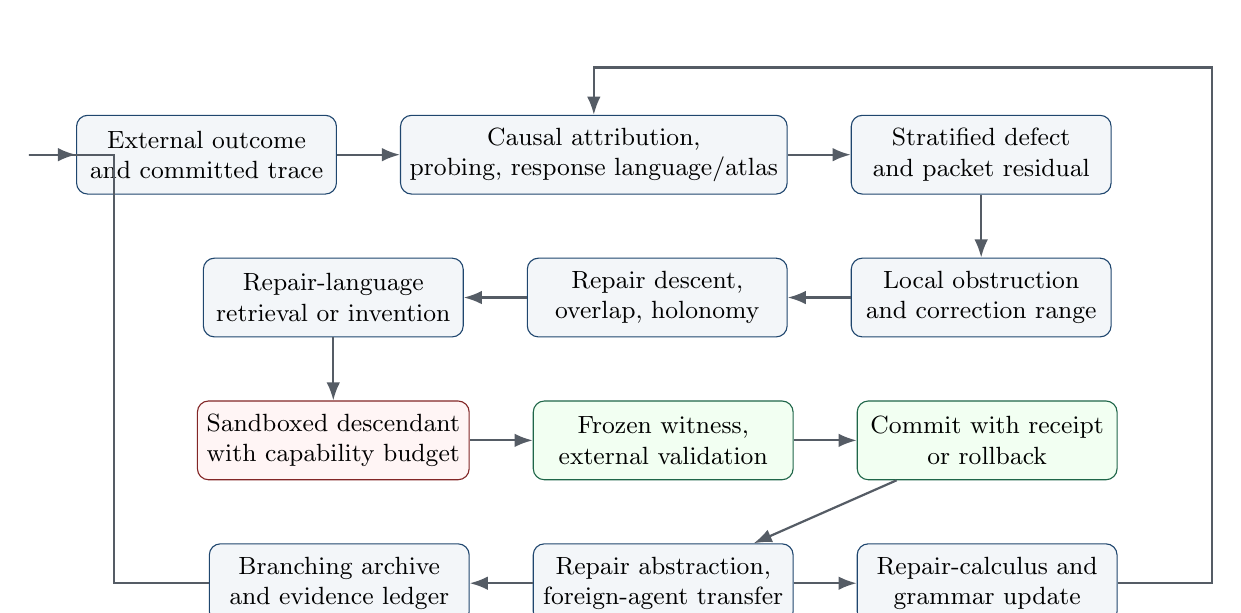
\begin{tikzpicture}[
  node distance=8mm and 8mm,
  box/.style={draw=KMBlue, rounded corners, align=center, minimum width=33mm, minimum height=10mm, fill=KMLight, font=\small},
  witness/.style={draw=KMGreen, rounded corners, align=center, minimum width=33mm, minimum height=10mm, fill=green!5, font=\small},
  risk/.style={draw=KMRed, rounded corners, align=center, minimum width=33mm, minimum height=10mm, fill=red!4, font=\small},
  arr/.style={-{Latex[length=2.3mm]}, thick, draw=KMGray}
]
\node[box] (outcome) {External outcome\\and committed trace};
\node[box, right=of outcome] (attrib) {Causal attribution,\\probing, response language/atlas};
\node[box, right=of attrib] (residual) {Stratified defect\\and packet residual};
\node[box, below=of residual] (obstruction) {Local obstruction\\and correction range};
\node[box, left=of obstruction] (descent) {Repair descent,\\overlap, holonomy};
\node[box, left=of descent] (schema) {Repair-language\\retrieval or invention};
\node[risk, below=of schema] (sandbox) {Sandboxed descendant\\with capability budget};
\node[witness, right=of sandbox] (validate) {Frozen witness,\\external validation};
\node[witness, right=of validate] (commit) {Commit with receipt\\or rollback};
\node[box, below=of validate] (abstract) {Repair abstraction,\\foreign-agent transfer};
\node[box, left=of abstract] (archive) {Branching archive\\and evidence ledger};
\node[box, right=of abstract] (meta) {Repair-calculus and\\grammar update};

\draw[arr] (outcome) -- (attrib);
\draw[arr] (attrib) -- (residual);
\draw[arr] (residual) -- (obstruction);
\draw[arr] (obstruction) -- (descent);
\draw[arr] (descent) -- (schema);
\draw[arr] (schema) -- (sandbox);
\draw[arr] (sandbox) -- (validate);
\draw[arr] (validate) -- (commit);
\draw[arr] (commit) -- (abstract);
\draw[arr] (abstract) -- (archive);
\draw[arr] (abstract) -- (meta);
\draw[arr] (meta.east) -- ++(12mm,0) coordinate (rloop) |- ($(attrib.north)+(0,6mm)$) -- (attrib.north);
\draw[arr] (archive.west) -- ++(-12mm,0) coordinate (lloop) |- ($(outcome.west)+(-6mm,0)$) -- (outcome.west);
\end{tikzpicture}%
}
\caption{The SRIC improvement loop. Controlled probes may first recover a functional response atlas before defects and repairs are localized. The witness path is separated from candidate construction. Successful repairs become reusable schemas, while valid obstructions and identifiability failures become reusable no-go certificates.}
\label{fig:sric-loop}
\end{figure}

\subsection{One transaction}

\begin{protocol}[Proof-carrying improvement transaction]
Given lineage state $\mathfrak L_t$:
\begin{enumerate}
\item Freeze witness $W_t$, evaluator core coordinates, evidence ledger head, resource budget, and rollback checkpoint.
\item Detect a persistent externally grounded mismatch.
\item Generate internal-change, world-change, sensor, memory, evaluator, copy, fork, and unknown hypotheses.
\item Select bounded active probes until uncertainty is below threshold or the probe budget is exhausted.
\item Estimate intervention-response operators and either replay a validated atlas or recover an endogenous functional cover with response-fit, commutator, spectral-gap, and identifiability certificates.
\item Resolve the defect into the validated local strata and compute local obstruction classes.
\item If a local obstruction is nonzero, record a no-go certificate and stop or extend the grammar.
\item Construct local repairs, compute overlap differences, and reject if the repair-descent class is nonzero.
\item Retrieve or construct a typed repair schema and estimate transport, leakage, and holonomy margins.
\item Precommit predicted gain and affected invariants.
\item Instantiate a sandboxed descendant with bounded capabilities.
\item Reveal external evaluation traces to the frozen witness.
\item Commit only if validation, provenance, regression, core-preservation, and rollback tests pass; otherwise restore the parent.
\item Abstract the result into a repair schema or obstruction certificate.
\item Test the abstraction on foreign held-out agents before adding it to the reusable repair operad.
\item Estimate remaining module-specific headroom and record any saturation certificate.
\item If current modules are saturated while persistent obstruction remains, issue a grammar-boundary receipt and begin conservative conflict refinement.
\item At the research-compiler level, test whether one diagnostic token contains incompatible sets of acceptable methods. If a conflict appears, search a declared generic experiment and constructor meta-language. Admit only a sealed conservative extension that improves foreign research problems.
\item At the Neuralese transport level, distinguish coordinate drift, nonlinear warp, latent-clock mismatch, chart aliasing, benign semantic quotient, and destructive information loss. Select the minimum passing constructor and issue no-go when protected semantics are not measurable from the target packet.
\end{enumerate}
\end{protocol}

\section{Empirical Status and Remaining Program}

\subsection{Realized in Block 5}

The released Block 5 reference package realizes the following finite and synthetic components:
\begin{enumerate}
\item the four-case local obstruction, gluing obstruction, flat repair, and evaluator-holonomy fixture;
\item universal, controlled, and productive closure checks on a finite transaction graph;
\item a witness-separated transaction kernel with commit, rollback, canonical receipts, and hash chaining;
\item a matched-model anonymous-change environment with bounded probes and abstention;
\item a matched-budget foreign-agent benchmark with static, search, packet, causal, transport, witness, and engineered meta positive-control arms;
\item a reproducible test, result, and manifest pipeline.
\end{enumerate}
These realizations support the mechanical and finite-semantic gates defined in \cref{sec:empirical-contract}. The anonymous and benchmark suites remain engineered positive controls rather than evidence of autonomous repair discovery.

\subsection{Realized in Block 6}

Block 6 replaces analytic hidden-coordinate transport by a controlled learned-representation problem. Its realized components are:
\begin{enumerate}
\item a causally defined hidden packet estimated from source intervention differences;
\item equal-rank PCA, random-packet, wrong-block, direct-copy, and shuffled-anchor controls;
\item a frozen packet-local source repair fitted without target audit labels;
\item a source-to-target bridge estimated from paired hidden activations while the constructing target map remains withheld;
\item seven target representation families spanning injective, overcomplete, ill-conditioned, compressed, mildly nonlinear, saturated, and piecewise-linear regimes;
\item independently trained linear and tanh encoders with distinct random initializations;
\item a frozen witness gate that can reject a blind target gain when alignment, protected competence, or unaffected-stratum regression is unacceptable;
\item a release-frozen package with disjoint train, anchor, calibration, and audit splits, five automated tests, a 34-file manifest, frozen result objects, and reproducible figures.
\end{enumerate}
The controlled package passes the cumulative foreign-transfer gate $G_{\rm foreign}$ for one shared task and defect grammar. It does not independently establish metaproductivity or grammar expansion.

\subsection{Realized in Block 7}

Block 7 implements two separately sealed parent--child comparisons of repair-process components.

\paragraph{Selection-only realization.}
The first route holds the ordered five-candidate repair bundle fixed on every target and changes only the commit policy. It realizes:
\begin{enumerate}
\item a frozen conservative parent selector;
\item a lineage-generated dual-head child selector fitted from development repair receipts;
\item a finite meta-grammar selected on a disjoint meta-validation split;
\item a descendant receipt sealed before either final audit is opened;
\item paired seed/task-foreign and architecture-foreign audits;
\item raw-calibration, no-risk, shuffled-lineage, selector-ablation, and audit-oracle controls;
\item identical non-null candidate budgets for every admissible selector arm.
\end{enumerate}
The child-parent protected-utility effects are
\begin{equation}
\widehat\Delta_{\rm audit}=0.072518,
\qquad
\widehat\Delta_{\rm arch}=0.104999,
\end{equation}
with positive frozen paired bootstrap intervals. Because parent and child share the same candidate set, this establishes behavioral selector metaproductivity but not expansion of the authorized correction image.

\paragraph{Bridge-policy realization.}
The second route holds the source repair, bridge family, transport formula, protected evaluator, and $24$-query deployment budget fixed while changing the paired-anchor selection rule and bridge-identification gate. It realizes:
\begin{enumerate}
\item a random-$16$ parent anchor policy;
\item a compiled pivoted-QR-$16$ descendant policy sealed before primary foreign targets are generated;
\item disjoint development and audit task families and disjoint primary representation families;
\item a $144$-target paired foreign audit and a separate stress suite;
\item random-budget, farthest-point, shuffled-binding, sign-flip, and plain-QR controls;
\item exact query ledgers, rank diagnostics, harm checks, and package-closed receipts.
\end{enumerate}
On the primary foreign audit, mean balanced selected gain rises from $0.135212$ to $0.344720$, and
\begin{equation}
\widehat\Delta_{\rm bridge}=0.209508,
\qquad
\mathrm{CI}_{95\%}=[0.194968,0.223898].
\end{equation}
Every primary paired effect is positive, full-rank bridge identification rises from $0.03125$ to $1$, and harmful selected targets remain zero. The plain pivoted-QR control is effectively identical, so the result supports rank-revealing query design rather than a packet-specific advantage.

The controlled packages therefore pass two distinct level-5 gates: $G_{\rm meta}^{\rm select}$ for selector metaproductivity and $G_{\rm meta}^{\rm bridge}$ for bridge-policy metaproductivity. Neither package establishes repeated-generation closure, autonomous candidate invention, or open-set grammar expansion.

\subsection{Realized in Block 8}

Block 8 is a formal and symbolic-realization expansion rather than a new learned-agent audit. It realizes:
\begin{enumerate}
\item finite restricted oracle envelopes and exact permutation-average meta-headroom allocation;
\item component saturation and headroom-adjusted metaproductivity;
\item bottleneck migration with an explicit conservative grammar-discovery coordinate;
\item nested obstruction images and exact newly correctable energy;
\item repair death versus forgetting death under dynamic defect semantics;
\item obstruction-guided one-generator and rank-$k$ grammar expansion;
\item finite repair-conflict refinement with a nuisance-feature negative control;
\item finite counterexample-guided repair synthesis or grammar exhaustion;
\item intervention-response algebra decomposition into central causal strata;
\item lineage-wide false-improvement and protected-regression budget accounting.
\end{enumerate}
The symbolic package passes eight automated tests and produces a package-closed result object and four figures. These fixtures validate the finite mathematics and its implementation. They do not advance the empirical claim ladder beyond the two one-step Block 7 metaproductivity results.


\subsection{Realized in Block 9}

Block 9 replays the exact Block 7 bridge child and compiles a fresh grandchild in a new heteroscedastic bridge environment. It realizes:
\begin{enumerate}
\item exact replay and digest verification of the Block 7 rank-revealing child policy;
\item fresh development and audit task supports and disjoint primary representation families;
\item a rank-saturation diagnosis in which every inherited primary design is full rank but its weighted information floor remains low;
\item a finite conditioning-aware policy grammar containing packet QR, unweighted D-optimal, quality-weighted D-optimal, quality-weighted A-optimal, and quality-weighted E-refined designs;
\item a quality-weighted D-optimal grandchild and a stronger recalibrated rank-child control;
\item identical $24$-query deployment budgets for the primary child and grandchild;
\item gate-only, quality-permutation, unweighted-design, random-$16$, and larger-budget random-$32$ controls;
\item a $96$-target paired primary foreign audit plus compressed, nonlinear, and severe-ill-conditioning stress families;
\item exact ancestor, compiler, pre-audit seal, result, query-ledger, and package-manifest receipts.
\end{enumerate}
On the fresh primary audit, mean selected protected gain rises from $0.037393$ for the recalibrated rank child to $0.209580$ for the conditioning grandchild. The paired effect is
\begin{equation}
\widehat\Delta_{1\to2}=0.172188,
\qquad
\mathrm{CI}_{95\%}=[0.141481,0.203110].
\end{equation}
Both designs have full-rank rate one. The mean weighted minimum information eigenvalue rises from $0.518197$ to $14.268195$, the median condition number falls from $19393.296$ to $544.180$, and clean transport NRMSE falls from $0.303981$ to $0.095803$. The gate-only and quality-permutation controls do not reproduce the selected gain. The release therefore passes a context-indexed two-edge repeated-lineage gate. It does not establish structural repair-grammar growth or improvement of the outer compiler.

\subsection{Realized in Block 10}

Block 10 retains the Block 9 quality-weighted acquisition mechanism but expands the representational grammar of repair transport. It realizes:
\begin{enumerate}
\item exact semantic replay of the Block 9 conditioning-aware ancestor;
\item a strengthened global-affine parent using $80$ fit plus $16$ witness pairs;
\item a conservative two-chart child using $48$ fit, $32$ chart-selection, and $16$ witness pairs;
\item one matched $96$-query deployment envelope for both processes;
\item a finite separator search restricted to the source repair's protected two-dimensional context packet;
\item a $54$-target development grammar-inadequacy certificate with full source rank, a persistent directly supervised global-affine residual, a near-exact true-chart oracle, smaller learned local residual, positive chart contrast, and an exact parent embedding;
\item disjoint development, meta-validation, and primary audit task and family identifiers;
\item a $96$-target primary foreign audit and a $32$-target stress suite;
\item direct global-affine oracle, global-blind, local-blind, gate-only, random-gate, shuffled-binding, and true-chart controls;
\item exact ancestor, compiler, grammar-certificate, pre-audit seal, result, test, figure, and package-manifest receipts.
\end{enumerate}
The resource-matched global parent abstains on the primary audit. The chart child obtains mean selected gain $0.334224$, median $0.284265$, commit rate $0.572917$, and zero harmful selected targets. The child-parent effect is
\begin{equation}
\widehat\Delta_{G\to C}=0.334224,
\qquad
\mathrm{CI}_{95\%}=[0.266459,0.401903].
\end{equation}
The sharper child-minus-direct-global-oracle effect is
\begin{equation}
\widehat\Delta_{\mathrm{oracle}\to C}=0.157530,
\qquad
\mathrm{CI}_{95\%}=[0.080863,0.234135].
\end{equation}
All primary source designs are full rank. Mean global validation NRMSE is $0.598513$, mean local validation NRMSE is $0.064975$, and mean learned gate accuracy is $0.874854$. Gate-only, random-gate, and shuffled-binding controls are strongly negative. Blind local application has higher mean gain but a nonzero harmful-commit rate, so the witness performs substantive selection. This passes the first finite structural repair-grammar gate. It does not establish autonomous packet, feature-language, chart-number, or compiler discovery.

\subsection{Current empirical interpretation}

The progression now separates seven empirical achievements and one formal bridge:
\begin{enumerate}
\item Block 5 realizes finite transactions, controls, and synthetic mechanics;
\item Block 6 realizes intervention-defined hidden packets and learned repair transport to foreign representations;
\item Block 7 realizes sealed one-step improvements of repair selection and rank-revealing evidence acquisition;
\item Block 8 formalizes meta-headroom, saturation, bottleneck migration, persistent obstruction, grammar refinement, causal-atlas discovery, and sequential lineage certification;
\item Block 9 replays the Block 7 child, diagnoses rank saturation, and realizes a second sealed edge by migrating to heteroscedastic conditioning-aware query design;
\item Block 10 holds that acquired query policy fixed, certifies that a global-affine repair family remains structurally obstructed, and realizes a conservative two-chart repair-transport extension;
\item the directly supervised global-affine oracle comparison separates function-class growth from a weak global estimator or permissive witness.
\end{enumerate}

The strongest admissible statement is:
\begin{center}
\emph{Within declared finite transport contexts, a proof-carrying lineage realizes two sequential query-policy improvements followed by one structural repair-grammar expansion. The final descendant retains conditioning-aware acquisition, proves a persistent residual for the global-affine repair family, conservatively adds an invariant-context chart-contrast direction, and improves fresh foreign targets under matched total evidence while preserving the global process as a fallback.}
\end{center}

The third edge crosses the boundary that Block 7 could not cross. The authorized opportunity set changes: two context-bound target repairs become reachable where the parent can instantiate only one global affine repair. The child also exceeds a directly supervised global-affine ceiling comparison. This is finite structural metaproductivity. It remains externally scaffolded because the protected packet, separator family, chart count, source repair, evaluator, witness, and outer compiler are supplied.

\subsection{Realized in Block 11}

Block 11 removes the protected context packet supplied to Block 10 and compiles a target-specific atlas from intervention responses. It realizes:
\begin{enumerate}
\item exact replay of the Block 10 ancestor policy and pre-audit lineage records;
\item a six-dimensional source with three hidden rank-two functional blocks under target-specific rotations or injective embeddings;
\item two controlled response operators with separating block signatures in the primary families;
\item central spectral block recovery up to permutation and within-block gauge;
\item response-fit, commutator, spectral-gap, commutant-dimension, and hidden-overlap audit diagnostics;
\item repair-relevant block labeling through source-repair invariance, target-gate agreement, local-bridge validation, chart balance, and protected regression;
\item a conservative executable embedding of the Block 10 supplied-packet grammar;
\item one equal $120$-query envelope for the inherited fixed-packet parent and endogenous-atlas child;
\item legacy-packet, PCA, full-space, random-atlas, shuffled-response, global, blind, and true-chart controls;
\item an $80$-target primary foreign audit and a $25$-target stress suite containing response degeneracy, strong coupling, smooth transitions, repair-dependent chart crossing, and compression;
\item exact compiler, atlas-certificate, pre-audit seal, result, figure, test, and $49$-file manifest receipts.
\end{enumerate}
The primary parent obtains zero selected gain and the child obtains $0.207325$. The paired effect has frozen interval $[0.131902,0.287910]$, no target favors the parent, and selected harm is zero. Blind child application has larger mean gain $0.271529$ but harm rate $0.1875$, so the witness performs substantive selection. The release passes a finite endogenous-atlas gate. It does not establish autonomous intervention invention, unrestricted block-count discovery, general noncommuting or nonlinear atlas recovery, or compiler self-improvement.


\subsection{Realized in Block 12}

Block 12 realizes two separately sealed structural edges beyond endogenous atlas recovery.
\paragraph{Response-language edge.}
The inherited two-operator response algebra contains an exact context--repair alias. Every polynomial and composition of inherited responses preserves the merged block. A finite intervention compiler selects one separating operator from five typed candidates, conservatively retains the old algebra, and seals the new response policy before a $96$-target foreign audit. Under equal $144$-query deployment budgets, selected protected gain rises from $0$ to $0.846985$, with frozen interval $[0.786100,0.901073]$, no negative paired effects, and zero selected harm.

\paragraph{Repair-constructor edge.}
After the response child identifies the repair packet, the inherited affine repair operad encounters a target correction with a nonzero quadratic Hessian. The child adds symmetric degree-two packet features while embedding every affine repair by zero quadratic coefficients. Under equal $160$-query deployment budgets, selected gain rises from $0.289123$ to $0.997511$. The paired effect is $0.708388$ with interval $[0.659635,0.757198]$, and the child exceeds a directly supervised $1600$-pair affine oracle by $0.530933$. A full-space quadratic control is equally effective, so the supported claim is degree-two constructor growth rather than unique block-local superiority.

These edges pass finite response-language and candidate-constructor gates. They do not establish unrestricted intervention invention, open-ended program synthesis, or improvement of the outer lineage compiler.


\subsection{Realized in Block 13}

Block 13 changes the research compiler while holding the downstream candidate-method grammar and final evaluator fixed. It realizes:
\begin{enumerate}
\item a strong parent compiler with structured literature priors, a shared finding graph, results-free receipts, exact code/specification binding, balanced exploration, multi-benchmark selection, capability gates, and integrity monitoring;
\item a child compiler trained only from development receipts, with a nearest-centroid obstruction classifier and ridge outcome/risk forecasters;
\item an identical $39$-method candidate grammar and identical six-full-experiment budget for parent and child;
\item development, meta-validation, primary foreign, and architecture-foreign problem splits with pre-audit compiler sealing;
\item shuffled-archive, classifier-only, forecaster-only, no-forum, single-benchmark, no-monitor, random-allocation, and audit-oracle controls;
\item exact proposal, code, archive, compiler, allocation, evaluator, monitor, result, test, and manifest receipts.
\end{enumerate}
On $96$ primary foreign problems, mean validity-filtered protected gain rises from $0.883004$ to $0.950231$, with paired effect $0.067227$ and frozen interval $[0.035881,0.103274]$. On $72$ architecture-foreign problems, gain rises from $0.772566$ to $0.863367$, with paired effect $0.090800$ and interval $[0.052311,0.135081]$. The obstruction classifier is the dominant realized mechanism. Outcome forecasting is informative but contributes only modestly, and removal of the finite within-problem forum has no measurable effect. The release passes a bounded research-compiler metaproductivity gate. It does not establish open-ended automated science, autonomous candidate-language growth, evaluator invention, or improvement of an unrestricted outer compiler.

\subsection{Realized in Block 14}

Block 14 replays the Block 13 result digest and exact method language, then recalibrates the inherited compiler design as the parent of an adversarial robustness study. It realizes:
\begin{enumerate}
\item diagnostic-matched clean and ambiguous problems that weaken one-shot obstruction classification;
\item sparse two-obstruction mixtures and an unknown class outside the inherited response cone;
\item evaluator-attack and integrity-attack method families;
\item an $18\%$ contaminated development archive plus a contamination sweep through $35\%$;
\item a robust child using sequential diagnosis, sparse response mixtures, open-set routing, robust archive summaries, evaluator portfolios, and an integrity-monitor ensemble;
\item the exact inherited $39$-method grammar and six-full-experiment budget for parent and child;
\item primary and independently shifted generator-foreign audits with pre-audit compiler sealing;
\item no-open-set, no-sequential, ordinary-archive, simple-monitor, single-portfolio, random-allocation, and audit-oracle controls;
\item exact results-free and post-result receipt chains, canonical results, tests, figures, and package manifest.
\end{enumerate}
On $144$ primary problems, mean validity-filtered protected gain rises from $0.410813$ to $0.575783$, with paired effect $0.164970$ and frozen interval $[0.115591,0.218655]$. On $120$ generator-foreign problems, gain rises from $0.389514$ to $0.550559$, with effect $0.161045$ and interval $[0.105335,0.223141]$. Primary lower-tail gain changes from $-0.133065$ to $0.271516$, observed invalid selections change from $0.027778$ to $0$, and false confident known-class assignment on unknown problems changes from $1$ to $0.083333$. Sequential response updating and open-set routing are substantively supported. The simple-monitor ablation is null and the single-portfolio ablation is nearly null, so neither receives independent positive attribution.

The claim remains finite. The child uses an externally declared response family, candidate grammar, attack vocabulary, evaluator portfolio, and monitor ensemble. It is a robustness improvement of the fixed-language compiler, not unrestricted open-set science or compiler-language growth.

\subsection{Realized in Block 15}

Block 15 replays the Block 14 result digest and promotes the robust compiler to the inherited parent of a structural compiler-language study. It realizes:
\begin{enumerate}
\item six inherited obstruction tokens, one undifferentiated unknown token, and the inherited $39$-method singleton grammar;
\item a development open-set cell containing two hidden research mechanisms that share the inherited diagnostic representation but require incompatible high-gain methods;
\item a generic six-probe research-experiment language and a generic $30$-member ordered pair-method constructor grammar;
\item finite conflict scoring, anonymous token refinement, pair-constructor synthesis, and exact conservative fallback;
\item hidden novel labels excluded from compiler construction and retained only for audit interpretation;
\item identical eight-unit deployment research budgets for parent and child;
\item primary and generator-foreign audits sealed after the language certificate and compiler object;
\item taxonomy-only, grammar-only, shuffled-binding, inherited-oracle, and expanded-oracle controls;
\item complete results-free and post-result receipts, deterministic figures, tests, and a package manifest.
\end{enumerate}
The development compiler selects \texttt{interaction-contrast} and binds the anonymous refined tokens to \texttt{evaluator-then-resource} and \texttt{objective-then-constructor}. The inherited development oracle obtains $0.377257$ mean open-set gain, while the selected extension obtains $0.948962$, producing a newly correctable margin $0.571704$.

On $96$ primary problems, mean protected gain rises from $0.633969$ to $0.859731$, with paired effect $0.225762$ and interval $[0.166708,0.286431]$. On $82$ generator-foreign problems, gain rises from $0.574224$ to $0.814520$, with paired effect $0.240296$ and interval $[0.180154,0.302701]$. No paired problem favors the parent. Known-class behavior is reproduced exactly through the inherited fallback. The taxonomy-only and shuffled-binding controls match the parent, while the grammar-only arm solves only the novel cell favored by its pooled binding. The release passes a finite compiler-language growth gate.

The result remains relative to an externally declared generic meta-language. The compiler does not invent arbitrary experiments or programs, semantically name the new obstruction classes, improve the evaluator or monitor, or execute real model-training research.


\subsection{Stage H completed: first repeated lineage}

The realized lineage is
\begin{equation}
K_0\xrightarrow{\Pi_1}K_1\xrightarrow{\Pi_2}K_2.
\end{equation}
The first edge improves rank identification. The second edge does not attempt to improve a saturated rank endpoint. It migrates to a distinct information-conditioning obstruction. Exact ancestor replay, new development evidence, a pre-audit grandchild seal, matched deployment queries, a recalibrated child control, and fresh foreign audit systems distinguish this result from reusing the Block 7 final evidence or weakening the parent.

A two-edge result is still finite. It does not imply a winning strategy for infinitely repeated productive closure, compiler self-improvement, or open-set grammar growth. It establishes that the lineage mechanism can produce a second successful descendant after the first improvement changes the active bottleneck.

\subsection{Stage I partially realized: finite structural grammar expansion}

Block 10 realizes the finite form of this stage. The lineage encounters foreign systems for which one global affine repair remains misspecified despite full-rank, quality-aware acquisition and an $80$-anchor parent fit. It records a grammar-inadequacy certificate, conservatively introduces an invariant-context two-chart constructor, and verifies a new anti-diagonal repair direction on fresh foreign systems. The stronger directly supervised global-affine oracle establishes that the gain is not explained by poor source-to-target bridge estimation alone.

Open-set grammar expansion additionally requires:
\begin{enumerate}
\item autonomous detection of a persistent obstruction or repair conflict;
\item invention or discovery of the separating feature, chart count, or nonlinear coordinate system;
\item a conservative embedding of old grammar, proofs, evidence, and authorization decisions;
\item exposure of a genuinely new correction direction under exact causal ablation;
\item held-out obstruction-energy reduction on foreign systems that require the new distinction;
\item preservation of evaluator, provenance, witness, and resource commitments;
\item repeated structural descendants under lineage-wide statistical and semantic-debt budgets.
\end{enumerate}
Block 10 supplies the obstruction, conservative extension, structural contrast, matched-resource audit, and causal controls. It does not by itself supply atlas discovery; Block 11 addresses one finite response-algebra form of that next requirement.

\subsection{Stage J partially realized: finite endogenous atlas growth}

Block 11 realizes the finite form of endogenous atlas growth. The supplied context packet is removed. A declared intervention family generates response operators whose central spectral blocks are recovered up to permutation and within-block gauge. Repair-validation evidence selects the block that supports a stable chart separator. The old supplied-packet process remains an executable subgrammar and fallback.

The unresolved part of Stage J is substantial. The intervention family, block dimensions, finite block-scalar response model, hard binary chart grammar, separator family, source repair, evaluator, witness, and outer compiler remain supplied. A stronger lineage must discover which intervention to run, whether signatures are degenerate, whether response operators are noncommuting, and whether the appropriate extension is another discrete block, a soft manifold, a kernel lift, or an information-loss certificate.

\subsection{Stage K completed in finite form: response-language and candidate-constructor growth}

Block 12 realizes the finite form of Stage K through two distinct contexts. The first edge certifies an exact response alias under the inherited algebra, selects one separating intervention from a fixed typed menu, and recovers a repair-enabling central refinement. The second edge certifies that every finite composition of inherited affine constructors remains affine while the target repair has a nonzero quadratic Hessian, then conservatively adds a degree-two constructor. Both results use matched query budgets, independent parent and child gates, fresh sealed audits, explicit function-class controls, and package-closed receipts.

The unresolved open-set form is stronger. A future lineage must enlarge the intervention or constructor language without receiving the final candidate menu, account for acquisition feasibility and physical effects, determine the necessary polynomial or program degree, and show that its outer diagnostic compiler transfers to foreign parent repair processes.

\subsection{Stage L partially realized: finite research-compiler metaproductivity}
Block 13 realizes a bounded improvement of the research-allocation compiler while the candidate-method language, evaluator portfolio, integrity monitor, and final research interfaces remain fixed. The child uses the same research budget more selectively by diagnosing the active obstruction and forecasting outcome and risk. This is an improvement of the process that generates and chooses repair-process descendants, but not an unrestricted improvement of its own language.

The unresolved form requires compiler grammar growth and eventually conservative evaluator evolution. A later compiler must detect that its obstruction taxonomy, proposal features, experimental actions, monitor, or evaluator portfolio is inadequate, introduce a new research distinction, preserve the path-flat evidential core, replay old protected decisions, and be witnessed by a component not rewritten in the same transaction. The primary danger is semantic capture through simultaneous alteration of proposal, evidence, utility, and approval.

\subsection{Stage M completed in finite form: adversarial open-set compiler robustness}

Stage M asks whether the finite research compiler remains useful after the clean six-way routing problem is replaced by ambiguous diagnostics, mixed obstructions, unknown cases, contaminated archives, evaluator attacks, integrity attacks, and a generator shift. Block 14 passes this finite gate. The child improves the inherited parent in mean and lower-tail validity-filtered gain under the same six-experiment budget, and every declared child group has positive mean gain. Some individual groupwise paired intervals include zero, so the aggregate and lower-tail claims are stronger than every family-specific claim.

The result does not yet satisfy the stronger external-robustness target. The benchmark generator, candidate methods, response language, attack types, evaluator portfolio, and monitor ensemble are still part of one package-closed research design. The next stage should combine an independently written generator and implementation with executable small-model or program-synthesis research, then require the robust compiler to issue a compiler-language inadequacy certificate before adding a new diagnostic, experiment, candidate family, or evaluator dimension.

\subsection{Stage N completed in finite form: compiler-language growth}

Stage N asks whether the robust research compiler can move beyond abstention or generic routing when its own diagnostic and method language is certified inadequate. Block 15 passes one finite form of this gate. One inherited open-set token contains development problems with incompatible acceptable-method sets. A finite compiler selects a separating probe from a generic experiment language, creates two anonymous refined tokens, synthesizes one ordered pair method for each token, and preserves the entire inherited compiler as an exact fallback.

This is structurally stronger than Block 14. The child does not merely classify known obstruction labels more robustly or allocate the inherited method grammar more effectively. It adds diagnostic and method expressions absent from the deployable parent language. The unresolved form is unrestricted compiler-language growth: the generic probe family, pair-composition operator, method primitives, evaluator, integrity monitor, and research simulator remain externally supplied.



\subsection{Stage O direct integration completed: Neuralese causal semantics}

Block 16 makes recurrent latent reasoning an explicit SRIC subsystem rather than an analogy. The latent transition, task-anchored update gate, halt map, trace convention, intervention language, semantic transport, and answer witness are separately typed and receipted. The mandatory audit distinguishes five possibilities: an inactive loop, an unordered loop, a corruption-fragile loop, a useful ordered but task-nonspecific loop, and a task-specific loop. Cross-task transplantation within fixed answer-format groups is the principal discriminator between the last two.

The companion validates the audit logic on a sealed synthetic parent--child pair. The parent passes necessity, order, corruption, and replay but fails task specificity, so its status is PARTIAL. The child raises structural-normalized specificity from $0.016952$ to $0.334610$, obtains a paired transplant-cost gain of $0.439986$ with interval $[0.386884,0.493143]$, preserves clean performance, and passes both the FULL causal and adaptive-halting gates. This is an engineered positive control, not evidence about a trained language model.

The local Hyper adapter is executable when the official runtime and weights are supplied. It imports the exposed injection hook, captures and reinjects exact latent states, computes gold-suffix cross-entropy through the official end-of-thought path, and emits canonical receipts. The actual model was not present in the build environment, so the real-model result remains open. The next empirical threshold is a sealed Hyper audit followed by a genuine parent--child checkpoint comparison generated by a declared training or search process.


\subsection{Stage P completed in finite form: executable Neuralese binding repair}

Block 17 realizes the two-checkpoint threshold proposed at the end of Block 16, but on a package-local recurrent micro-model rather than Hyper. A separately implemented exact rational environment generates affine programs and protected $(A,B,y)$ witnesses. A task-blind trained parent is inherited into six finite repair candidates. The compiler uses only development, meta-validation, and probe-calibration evidence, seals the selected checkpoint, and then faces fresh primary and shifted-generator tasks.

The first sealed attempt is negative: the selected child improves absolute transplant effects and semantic decodability but misses the frozen normalized FULL gates. The package retains that failure and commits a revision before new final-task generation. In the second round, three candidates are eligible and the full-binding child is selected. The parent remains structurally active but program blind. The child passes necessity, order, noise, replay, program specificity, answer specificity, local semantic continuity, donor coverage, external trace decoding, and adaptive-depth gates on both final supports. The accepted receipt is \texttt{6cc2257f...655e4ae}.

This closes one finite training-generated latent-binding edge. It does not establish foreign-model metaproductivity.

The affine task family, semantic witness, donor taxonomy, candidate ranks, loss, compiler score, and gate thresholds remain external. The decisive next test is an independently trained latent-reasoning architecture or a real parent--child production checkpoint pair, preferably with a compiler-generated modification absent from the Block 17 grammar.


\subsection{Stage Q attempted and obstruction-certified: cross-implementation Neuralese transport}

Block 18 instantiates the source-selected progressive FiLM schema in two independently implemented recurrent cell families. On the primary generator, both selected children satisfy the full causal, semantic, execution, replay, and adaptive-depth gates. The stronger family claim fails under the shifted generator. Both external semantic probes become negative, exact execution falls below $0.09$, adaptive depth collapses, clean loss regresses, and both frozen latent bridges fail even though their anchor trace matrices are full rank and their pre-audit transported $R^2$ values exceed $0.70$.

The failure is retained as a semantic-chart obstruction rather than interpreted as absence of every latent semantic variable. After the canonical receipt is frozen, a separate held-out split diagnosis refits only shift-local readouts and bridges. Source and target probes recover $R^2$ between $0.574$ and $0.601$, paired bridges recover $0.539$ to $0.555$, and shuffled bridges remain negative. Thus the next missing object is a context-indexed or invariant semantic atlas with abstention, not another static full-rank bridge. No transition $\Pi_{18}$ is accepted in this revision.

\subsection{Stage R completed in finite form: distribution-indexed source atlas growth}

Block 19 acts on the Block 18 chart obstruction before attempting another foreign bridge. It compiles two new observation charts from protected semantic twins, preserves the four inherited charts exactly, separates the recurrent semantic path from the context-diagnostic path, and rejects nonlinear contexts outside the authorized affine grammar. The selected child is \texttt{ATLAS\_FULL} on fresh inherited and added-chart supports.

\subsection{Stage S completed in finite form: atlas-indexed cross-architecture transport}

Block 20 transports the stabilized six-chart bundle from independently trained GRU and gated-residual trajectories into the frozen Elman source representation. One full-trajectory map is selected per architecture and admitted chart. The connection preserves the source semantic readout, reduces architecture--context curvature below the frozen ceiling, defeats pooled and shuffled-binding controls, and retains selective rejection outside the atlas.

\subsection{Stage T completed in finite form: obstruction-guided transport-grammar growth}

Block 21 changes the response language of the transport process. The compiler is not given the obstruction-family label. It must infer whether the inherited connection faces ordinary affine drift, smooth nonlinear warp, latent-clock mixing, an aliased chart, benign rank loss, or protected semantic destruction. It then selects the minimum-description passing constructor or a collision-grounded no-go certificate. All $36$ fresh final episodes receive the required response across both foreign architectures.

The result remains finite. The packet, obstruction families, response probe, protected semantic coordinates, constructor grammar, and paired calibration interface remain declared. The accepted edge does not establish unrestricted natural-model diagnosis.

\subsection{Precommitted next-stage estimands}

The next major study should test \emph{unpaired and ontology-light Neuralese transport}. It should precommit:
\begin{enumerate}
\item exact replay of the Block 19 atlas, Block 20 connection, Block 21 compiler seal, final family receipt, and independent verifier;
\item removal of exact source--target task pairing from transport fitting;
\item sparse protected anchor orbits, controlled interventions, or output-equivalence classes as the only shared landmarks;
\item candidate semantic operators proposed from response regularities rather than a complete author-supplied intermediate-state ontology;
\item explicit tests for gauge-equivalent descriptions, strategy multimodality, and genuinely different computations;
\item variable-length or stochastic recurrent trajectories with chronology-preserving transport;
\item no-go certificates when the shared observations do not identify a protected semantic correspondence;
\item independent task generation, fresh architecture families, and sealed primary and generator-foreign audits;
\item lower-tail, coverage, abstention, resource, and protected-regression estimands;
\item append-only retention of every failed pilot and every protocol change before final-support generation.
\end{enumerate}
A full SRIC claim remains factorized. No aggregate score may replace validity, causal relevance, semantic sufficiency, obstruction diagnosis, conservative grammar growth, evaluator adequacy, independent replication, and open-set gates.

\section{Conditional Stratified Recursive Improvement Theorem}

\begin{conditionaltheorem}[Conditional SRIC theorem, Block 21 form]
\label{thm:umbrella}
Consider a finite declared agent atlas and a sequence of lineage states $\mathfrak L_t$. Assume:
\begin{enumerate}
\item externally grounded outcome traces and an append-only evidence ledger;
\item typed authorized correction spaces, defect maps, and local obstruction computation;
\item effective repair descent on the declared cover;
\item coherent repair transport with pathwise norm, authorization, and obstruction-faithfulness bounds;
\item a nontrivial adequate evaluator core and conservative evaluator morphisms;
\item witness-separated transactions with a decision-complete trace, sandboxed effects, precommitment, and rollback;
\item a finite transaction game with declared actions and admissible outcomes;
\item an append-only receipt-closed archive;
\item calibrated acceptance with summable conditional false-acceptance budgets;
\item conservative grammar embeddings on the protected fragment;
\item foreign-agent evaluation under matched resources;
\item for the autocatalytic clause, a valid finite-type branching approximation with a causally identified offspring matrix;
\item an executable runtime with a declared abstraction map, observation-commuting refinement, canonical receipt compiler, frozen endpoints, and package-closed evidence;
\item cumulative empirical claim gates whose interpretation is restricted to the highest gate that passes;
\item for learned representation transfer, disjoint train, anchor, calibration, and audit samples, a declared causal intervention, a frozen source repair, paired-anchor-only bridge fitting, and no target-audit or target-oracle leakage into candidate construction;
\item for statistical witness guarantees, simultaneous calibration-to-audit deviation bounds for gain, protected regression, and transport quality;
\item for selector-level metaproductivity, a lineage-generated child sealed from development and meta-validation evidence before final audit access, pathwise identical candidate bundles, fixed protected utility, matched candidate and evidence budgets, and a predeclared paired inference rule;
\item for bridge-policy metaproductivity, a lineage-generated repair process sealed before primary audit generation, pathwise matched source repair and deployment query budgets, disjoint development and primary family supports, exact query ledgers, a fixed transport-and-evaluation mechanism, and a predeclared paired inference rule;
\item for repeated recursive closure, fresh evidence and valid witness separation at every lineage generation;
\item for module-specific headroom claims, a declared repair-process factorization and valid restricted oracle envelopes or certified bounds;
\item for bottleneck migration, a saturation-aware controller and a weighted local contraction certificate inside each fixed grammar;
\item for structural grammar growth, obstruction-faithful semantic transports, held-out obstruction measurements, and causal ablation of every new generator;
\item for conflict-grounded grammar refinement, a finite externally validated repair-conflict family and a declared feature or probe family;
\item for causal-atlas claims, a finite adjoint-closed response algebra or a spectrally separated empirical approximation;
\item for lineage-wide statistical claims, conditional edge-level coverage with summable false-acceptance and protected-regression budgets;
\item for heteroscedastic bridge claims, conditionally independent paired-anchor noise with declared or validly estimated quality weights and a fixed weighted bridge estimator;
\item for conditioning-aware query claims, matched deployment query budgets, a finite pre-audit design grammar, and controls that isolate query design from gate recalibration and quality-label shortcuts;
\item for the Block 9 repeated-lineage claim, exact ancestor receipt replay, fresh development and final audit supports, a sealed grandchild, a recalibrated child control, and a context-indexed interpretation of the two edges;
\item for the Block 10 structural grammar claim, full-rank inherited designs, a strengthened global parent, a persistent directly supervised global-affine residual, a conservative embedding into the chart grammar, a nonzero chart-contrast direction, a matched total query envelope, fresh paired foreign evaluation, and gate-only, random-gate, shuffled-binding, blind-local, and stress controls.
\item for the Block 11 endogenous-atlas claim, exact ancestor replay, removal of the supplied context packet, a declared intervention-response family, target-specific hidden rotations, separating response signatures or a certified abstention condition, matched total effect-query budgets, a conservative Block 10 fallback, fresh paired foreign evaluation, and PCA, full-space, random-atlas, shuffled-response, blind, and stress controls;
\item for the Block 12 response-language claim, an inherited exact or statistically certified response alias, a finite pre-audit intervention candidate language, a separating signature margin, conservative algebra embedding, matched total query budgets, fresh foreign evaluation, and duplicate, weak, shuffled, random-atlas, and stress controls;
\item for the Block 12 constructor claim, an inherited affine repair operad, a nonzero-Hessian or equivalent function-class obstruction, a conservatively embedded finite constructor language, matched total query budgets, separately compiled parent and child witnesses, a same-target affine function-class control, and wrong-block, random-block, shuffled-feature, full-quadratic, and stress controls;
\item for the Block 13 research-compiler claim, identical initial archives, candidate-method grammars, evaluator portfolios, integrity monitors, proposal and full-experiment budgets, results-free receipts sealed before outcomes, disjoint development, meta-validation, primary, and architecture-foreign research problems, a pre-audit compiler seal, and paired validity-filtered final audits with declared mechanism controls.
\item for the Block 14 robust-compiler claim, exact Block 13 ancestor replay, identical fixed method grammars and six-experiment budgets, diagnostic aliasing and sparse mixture families, a declared unknown-response margin, contaminated development receipts, finite evaluator and integrity attacks, pre-audit compiler sealing, group-resolved and lower-tail gates, and a separately shifted generator-foreign audit.
\item for the Block 15 compiler-language claim, exact Block 14 ancestor replay, an inherited unknown token containing an externally validated method conflict, a finite generic probe language, a finite generic method-constructor grammar, hidden novel labels excluded from compilation, an exact inherited fallback, matched eight-unit deployment budgets, pre-audit language and split sealing, and taxonomy-only, grammar-only, shuffled-binding, inherited-oracle, and expanded-oracle controls.
\item for the Block 16 Neuralese claim, an explicitly located latent injection hook, a fixed trace convention, identical prompt and answer scoring across arms, zero-step, replay, permutation, norm-matched-noise, and same-format transplant interventions, matched latent-step budgets, sealed task and donor digests, and a frozen external witness.
\item for the Block 17 executable Neuralese repair claim, exact external task witnesses, one inherited trained parent, matched candidate optimization envelopes, same-answer far-program and far-answer matched-depth donors, an independently fit trace probe, adaptive-depth gates, a preserved failed pilot, a precommitted revision, a compiler seal before fresh final-task generation, and package-local NumPy, receipt, witness, and gauge replay.
\item for the Block 18 obstruction claim, independently implemented foreign recurrent cells, exact ancestor replay, a source-selected repair schema, primary and shifted audits, frozen semantic bridges, and post-audit localization kept outside acceptance;
\item for the Block 19 atlas claim, protected semantic twins, a sealed finite chart grammar, exact inherited fallback, selective admission, fresh supported and unsupported contexts, and independent route and forward verification;
\item for the Block 20 connection claim, a frozen source atlas, independently trained foreign targets, chart-indexed gauge stress, a pre-audit transport compiler, complete trajectory and curvature audits, shuffled binding, and unsupported-context controls;
\item for the Block 21 transport-grammar claim, a frozen diagnostic packet and semantic witness, hidden obstruction-family labels, a finite typed repair grammar, minimum-description eligibility, disjoint episode splits, collision-grounded no-go, fresh foreign audits, and exact independent replay.
\end{enumerate}
Then:
\begin{enumerate}
\item local correctability, nonlinear lifting, and global repair descent obey the results of the earlier blocks;
\item exact and approximate repair transport obey the stated equivalence, accumulation, and gain-margin theorems;
\item conservative evaluator chains preserve recoverable protected evidence and every decision above the cumulative stability margin;
\item direct atomic self-approval is excluded relative to the declared trace, and rejected buffered transactions restore the sealed parent;
\item the universal recursive closure, robust controlled kernel, and productive nested fixed point exist and are computable in the finite model;
\item the archive's scalar upper envelopes are nondecreasing under append-only retention, and an $\eps$-Pareto cover of bounded size exists;
\item only finitely many harmful acceptances occur almost surely under the summable error condition;
\item nested repair images reduce held-out obstruction energy by exactly the defect energy in newly correctable directions;
\item every finite old proof persists along the conservative grammar chain, and ontology expansion satisfies the old-resolution and new-obstruction exact sequence;
\item finite repair-discovery closure exists, while the branching threshold and spectral certificates hold under their additional stochastic assumptions;
\item every covered executable trace maps to an authorized abstract trace with matching protected observations, and exhaustive finite endpoints are decidable when exact realization holds;
\item package integrity, mechanics, finite semantics, causal identification, foreign transfer, selector metaproductivity, structural metaproductivity, repeated recurrence, and open-set recursion remain distinct claims and are admissible only through their cumulative gates;
\item in the linear Block 6 fixture, intervention differences recover the exact causal packet under the covariance condition of \cref{thm:block06-linear-packet};
\item an exact injective hidden bridge transports the source repair equivariantly by \cref{thm:block06-exact-transport}, while a noninjective bridge leaves the explicit compression residual of \cref{prop:block06-compression-residual};
\item a candidate passing a tightened witness gate has positive audit gain and respects the declared audit regression and alignment bounds whenever the simultaneous deviation assumptions of \cref{thm:block06-witness-soundness} hold;
\item a sealed child selector satisfying the hypotheses of \cref{thm:block07-one-step} is a certified one-step bounded improvement of the repair-selection process;
\item if parent and child share the same candidate bundle, that selector-level certificate does not imply structural repair-image growth by \cref{prop:block07-fixed-candidate-invariance};
\item a sealed bridge-policy child satisfying \cref{thm:block07q-one-step-certificate} is a certified one-step bounded improvement of paired-anchor query design and bridge identification relative to the declared finite benchmark;
\item a single productive child edge does not imply recurrent productive closure without a fresh successful descendant edge;
\item finite restricted oracle envelopes allocate total declared headroom exactly across repair-process modules, and an $\eps$-saturated module coalition cannot support more than $\eps$ additional gain;
\item under the Block 8 Lyapunov hypothesis, weighted module headroom contracts during fixed-grammar intervals while the target of improvement may migrate among modules;
\item nested grammar correction images reduce obstruction energy by exactly the component in newly correctable directions;
\item finite repair-conflict refinement terminates when the candidate feature family separates every minimal conflict;
\item a finite adjoint-closed intervention algebra has a canonical central causal atlas up to multiplicity gauge;
\item summable conditional edge budgets control the probability of accepting any false lineage improvement across an adaptive finite or countable archive;
\item weighted least squares has coefficient covariance $I_q\otimes M_S^{-1}$ under the Block 9 noise model, so full rank without a positive information floor is insufficient for stable bridge recovery;
\item a conditioning-aware query policy satisfying the Block 9 sealed paired certificate is a bounded improvement over the recalibrated rank child in the declared fresh context;
\item the verified sequence $K_0\xrightarrow{\Pi_1}K_1\xrightarrow{\Pi_2}K_2$ is a finite two-edge context-indexed repeated-lineage realization, but not a same-context scalar transitivity result or an infinite productive-closure certificate;
\item under the Block 10 chart assumptions, a positive global residual margin together with a nonzero chart repair contrast certifies a correction direction unavailable to the inherited diagonal global grammar;
\item a Block 10 descendant satisfying \cref{thm:b10-finite-realization} is a bounded structural repair-grammar improvement relative to the declared piecewise foreign benchmark.
\item under separating block-scalar response signatures, the hidden central projectors are polynomials in a generic response combination and are identifiable up to block permutation and within-block gauge by \cref{thm:b11-exact-atlas};
\item a Block 11 descendant satisfying \cref{thm:b11-realization} is a finite endogenous-atlas improvement relative to the declared intervention-response benchmark;
\item under an inherited response alias, every polynomial composition of the old response operators preserves the alias, while a separating operator satisfying \cref{thm:b12-central-refinement} creates a new identifiable central block;
\item a Block 12 response child satisfying \cref{thm:b12-response-realization} is a finite response-language expansion under the declared matched-resource benchmark;
\item a nonzero-Hessian target repair is unavailable to the affine repair operad by \cref{thm:b12-affine-closure,thm:b12-hessian-obstruction};
\item a Block 12 constructor child satisfying \cref{thm:b12-constructor-realization} is a finite candidate-constructor expansion relative to the declared degree-two benchmark;
\item a Block 13 child compiler satisfying \cref{thm:b13-realization} is a finite matched-budget improvement of the proof-carrying research compiler relative to the fixed research-problem distribution, method grammar, evaluator portfolio, and integrity model.
\item a Block 14 child satisfying \cref{thm:block14-realization} is a finite matched-budget robustness improvement of that compiler relative to the declared diagnostic-aliasing, multi-obstruction, open-set, contamination, evaluator-shift, and integrity-attack atlas.
\item a Block 15 child satisfying \cref{thm:block15-realization} is a finite matched-budget compiler-language expansion that conservatively refines one inherited unknown token and adds task-relevant method constructors absent from the deployable parent grammar.
\item a Block 16 child satisfying \cref{thm:b16-neuralese-edge} is a finite evidence-preserving improvement of the recurrent latent-reasoning component; it becomes an improvement-process edge only when the child-producing mechanism itself generated the accepted latent modification.
\item a Block 17 child satisfying \cref{thm:b17-executable-edge} is a finite training-generated repair of the Neuralese binding component on the declared exact environment; it remains distinct from foreign-model or open-ended repair-language metaproductivity.
\item the Block 18 result is a valid sealed obstruction certificate rather than an accepted positive edge;
\item a Block 19 child satisfying \cref{thm:b19-realization} is a conservative source-side semantic-atlas expansion on the declared context family;
\item a Block 20 connection satisfying \cref{thm:b20-realization} is a finite atlas-indexed cross-architecture transport edge with bounded architecture--context curvature;
\item a Block 21 compiler satisfying \cref{thm:b21-realization} is a finite evidence-preserving expansion of the transport response grammar that distinguishes correctable map classes from protected information loss.
\end{enumerate}
Blocks 10 through 12 instantiate successive finite repair-language cases of the theorem's structural clause, Block 15 instantiates the corresponding compiler-language clause, Block 16 instantiates a directly intervenable recurrent latent-language clause, Block 17 instantiates one training-generated executable latent-binding repair, Block 18 records a distributional obstruction, Blocks 19 and 20 construct a semantic atlas and connection, and Block 21 expands the transport response grammar: first a supplied-packet chart grammar, then a target-specific response-derived atlas, then refinement of the response language itself and expansion of the repair-constructor function class. If, in addition, later descendants autonomously expand the feature, atlas, or repair-constructor grammar, expose further task-relevant correction directions, reduce held-out obstruction energy, preserve old proofs and evaluator commitments, and improve foreign systems under newly sealed matched-resource audits, then those later edges form a conservatively growing structural recursive lineage. An unbounded or indefinitely accelerating conclusion requires further recurrence, resource, grammar, and evaluator hypotheses not established here.
\end{conditionaltheorem}

\begin{proof}
Items 1 through 3 collect the established correction, descent, transport, and evaluator results. Item 4 follows from \cref{thm:witness-noninterference,thm:trace-factorization,thm:atomic-rollback}. Item 5 follows from \cref{thm:ri-closure,thm:controlled-closure,thm:productive-closure}. Item 6 follows from \cref{prop:archive-envelope,thm:epsilon-pareto-cover}. Item 7 is \cref{thm:adaptive-alpha-spending,thm:summable-errors}. Item 8 is \cref{thm:structural-behavioral}. Item 9 follows from \cref{thm:grammar-preservation,thm:grammar-colimit,thm:dynamic-obstruction-exact}. Item 10 follows from \cref{thm:discovery-closure,thm:branching-threshold,thm:spectral-interval}. Item 11 follows from \cref{thm:runtime-trace-soundness,thm:finite-endpoint-complete}. Item 12 follows from the cumulative claim-gate definition in \cref{sec:empirical-contract} together with the Block 7 distinction between selector and structural gain. Items 13 through 15 are \cref{thm:block06-linear-packet,thm:block06-exact-transport,prop:block06-compression-residual,thm:block06-witness-soundness}. Item 16 is \cref{thm:block07-one-step}. Item 17 is \cref{prop:block07-fixed-candidate-invariance}. Item 18 is \cref{thm:block07q-one-step-certificate}. Item 19 follows because existence of one productive transition supplies no winning strategy or fixed-point witness for infinitely repeated progress. Items 20 through 25 follow from \cref{thm:b8-shapley-efficiency,prop:b8-component-ceiling,thm:b8-lyapunov,thm:b8-new-energy,thm:b8-conflict-refinement,thm:b8-atlas-decomposition,thm:b8-lineage-validity}. Item 26 is \cref{thm:b9-wls}. Item 27 follows from \cref{thm:b9-dopt} together with the sealed Block 9 paired audit. Item 28 is the finite two-edge realization theorem of \cref{sec:block09-results}. The Block 10 structural items follow from \cref{thm:b10-open-set-obstruction,prop:b10-conservative-embedding,prop:b10-repair-contrast,thm:b10-finite-realization}. The Block 11 atlas items follow from \cref{thm:b11-exact-atlas,thm:b11-commutant,thm:b11-spectral-stability,thm:b11-block-selection,prop:b11-conservative,prop:b11-fixed-insufficiency,thm:b11-realization}. The Block 12 response-language items follow from \cref{thm:b12-alias-persistence,thm:b12-central-refinement,prop:b12-response-perturbation,thm:b12-response-realization}; the constructor items follow from \cref{thm:b12-affine-closure,thm:b12-hessian-obstruction,thm:b12-gaussian-affine-residual,prop:b12-affine-embedding,prop:b12-quadratic-gauge,thm:b12-constructor-realization}. The Block 13 compiler items follow from the results-free receipt construction, evaluator-nullspace refinement theorem, forecast-regret theorem, paired compiler certificate, and \cref{thm:b13-realization}. The Block 14 robustness item follows from \cref{thm:static-diagnostic-indistinguishability,prop:response-mixture-bound,prop:open-set-separation,prop:evaluator-nullspace-refinement,prop:monitor-bound,thm:block14-realization}. The Block 15 compiler-language item follows from \cref{thm:b15-routing-obstruction,thm:b15-diagnostic-refinement,thm:b15-language-synthesis,prop:b15-method-embedding,thm:block15-realization}. The Block 16 Neuralese item follows from \cref{thm:b16-transplant-null,prop:b16-replay,prop:b16-exact-transport,thm:b16-neuralese-edge}. The Block 17 through 21 items follow from their sealed realization theorems and obstruction certificates, including \cref{thm:b17-executable-edge,thm:b19-realization,thm:b20-realization,thm:b21-realization}. The final statement combines conservative grammar extension, structural correctability gain, matched foreign evaluation, bottleneck migration, repeated-lineage certification, sequential validity, and the preserved transaction invariants.
\end{proof}



\section{Failure Modes and Falsification Criteria}

A useful theory should specify observations that weaken or refute its proposed mechanisms.

\begin{enumerate}[label=\textbf{F\arabic*.}]
\item \textbf{Trace incompleteness.} Adversarially different full executions repeatedly collapse to one declared trace while requiring different witness decisions.
\item \textbf{Rollback failure.} Rejected candidates leave undeclared operational effects or cannot restore the sealed parent.
\item \textbf{Circular witness replacement.} A purported rotating schedule contains an unavoidable validation cycle without an external witness or preserved old validator.
\item \textbf{Safe-no-op false positive.} The system reports recursive improvement when it lies only in the safety closure and cannot force repeated gain events.
\item \textbf{Closure-model mismatch.} Fixed-point certificates fail to predict actual invariant violations or omit admissible transitions that occur in execution.
\item \textbf{Archive option-value failure.} Multiobjective retention and continuation signatures do not improve future reachability over simpler greedy or random archives after matched storage and compute.
\item \textbf{Best-of-$k$ confound.} Apparent metaproductivity disappears when candidate count, compute, tools, and validation access are matched.
\item \textbf{No foreign transfer.} Improvement lift is confined to descendants or systems used during mechanism design.
\item \textbf{Structural irrelevance.} Repair rank grows while held-out obstruction energy and task loss do not improve.
\item \textbf{No causal gain from stratification.} Packet-localized repairs do not outperform matched global-edit baselines.
\item \textbf{Transport bound nonpredictive.} Measured transport, leakage, and holonomy errors do not predict target repair success beyond generic distribution-distance baselines.
\item \textbf{Evaluator-core failure.} Protected evidence semantics drift despite low computed holonomy, or the retained core has negligible adequacy.
\item \textbf{Nonconservative grammar growth.} New types silently alter old evidence, proof meaning, or authorization strength.
\item \textbf{No representational boundary signal.} Claimed grammar inadequacy pairs are separable by the old grammar or do not require distinct repairs.
\item \textbf{Noncausal offspring.} Repair-offspring edges disappear under necessity ablation, matched evidence, or shared-compute controls.
\item \textbf{Autocatalytic overclaim.} A spectral radius above one disappears under a simultaneous lower confidence matrix, resource normalization, equivalence-class compression, or saturation controls.
\item \textbf{No advantage over ordinary search.} A simpler archive-based optimizer matches the full architecture on every precommitted primary endpoint.
\item \textbf{Implementation-refinement failure.} Runtime traces violate the abstract transition relation, protected observations do not commute, or receipts compile inconsistently.
\item \textbf{Oracle leakage.} Hidden defect labels, target repairs, evaluator truth, or foreign-test outcomes enter candidate construction or threshold selection.
\item \textbf{Fixture-only success.} Positive results disappear when analytic prototypes, exact transports, or hand-coded schemas are removed.
\item \textbf{Seed fragility.} The frozen smoke seed passes while independent statistical replays fail the preregistered gates.
\item \textbf{Manifest incompleteness.} Undeclared executable files, mutable dependencies, or external services alter the result without changing the released manifest.
\item \textbf{Claim-gate inflation.} A mechanical or finite-semantic pass is described as causal, metaproductive, or open-set evidence without satisfying the intervening gates.
\item \textbf{Causal-packet null.} The intervention-defined packet fails to outperform equal-rank PCA, random, and wrong-block controls under matched fitting resources.
\item \textbf{Anchor irrelevance.} Shuffling source-target anchor correspondence does not materially reduce transfer, indicating that the learned bridge is not using paired semantics or that the task admits a shortcut.
\item \textbf{Unsafe blind transport.} Blind target gain remains high while protected-stratum quality collapses, and the declared witness nevertheless commits.
\item \textbf{Obstruction-blind alignment.} State alignment residuals are small, but repair-equivariance residuals and protected loss remain large without being detected by the transport certificate.
\item \textbf{Shared-bottleneck confound.} Transfer disappears when the reconstruction objective, shared feature generator, or supplied causal block is removed, showing that the learned pilot depended on engineered representational alignment.
\item \textbf{Foreignness collapse.} Target encoders, target seeds, audit examples, or target-local repair information leak into source repair discovery or witness-threshold selection.
\item \textbf{Seal violation.} Final audit receipts, audit-derived features, or audit-selected thresholds enter child compilation before the descendant receipt is fixed.
\item \textbf{Selector attribution failure.} The child advantage disappears when parent and child receive the identical ordered candidate bundle and identical evidence.
\item \textbf{Lineage-binding null.} Correct and shuffled development receipts produce indistinguishable held-out child behavior.
\item \textbf{Risk-head vacuity.} The protected child and no-risk child have indistinguishable risk profiles, or the declared risk head fails to prevent the violations it was introduced to control.
\item \textbf{One-edge overclaim.} A single positive parent--child edge is described as repeated recursive closure without a fresh child--grandchild result.
\item \textbf{Fixed-candidate structural overclaim.} Selector improvement is reported as expansion of the correction image even though the authorized candidate set is unchanged.
\item \textbf{Meta-validation collapse.} The chosen child fails both disjoint final audits after a large finite meta-grammar search.
\item \textbf{Headroom miscalibration.} A module is declared saturated while a matched admissible oracle or later sealed child reveals substantial remaining opportunity.
\item \textbf{Bottleneck-stasis overclaim.} Repeated descendants modify the same saturated component while unresolved foreign obstruction has migrated elsewhere.
\item \textbf{Discovery-as-regression error.} A conservative grammar extension is rejected solely because it reveals a new validated defect coordinate.
\item \textbf{Forgetting death.} An obstruction class disappears only because the new semantic transport collapses the protected distinction.
\item \textbf{Generator irrelevance.} A proposed new repair generator has no component outside the old correction image or its gain survives exact generator ablation.
\item \textbf{Conflict-feature shortcut.} A selected grammar feature predicts development labels but does not resolve incompatible authorized repairs on foreign episodes.
\item \textbf{Atlas instability.} Small perturbations of intervention-response operators cause uncontrolled changes in the recovered atlas because the required spectral gap is absent.
\item \textbf{Compiler-process conflation.} Improvement of one compiled repair process is reported as improvement of the outer lineage compiler without a foreign-parent compiler audit.
\item \textbf{Sequential-budget failure.} Repeated descendant claims reuse evidence or exceed their cumulative false-acceptance, regression, or semantic-debt budgets.
\item \textbf{Rank-only repeated-lineage overclaim.} A purported grandchild changes only the gate or repeats rank recovery after full-rank saturation without improving information conditioning or transport quality.
\item \textbf{Quality-binding null.} Permuting the anchor-quality metadata leaves the grandchild design, information floor, and selected foreign gain unchanged.
\item \textbf{Gate-only attribution.} Applying the grandchild witness gate to inherited rank anchors reproduces the grandchild result.
\item \textbf{Stale-parent comparison.} The reported grandchild advantage exists only against the unchanged Block 7 gate and disappears against a development-recalibrated rank child.
\item \textbf{Query-budget mismatch.} The grandchild uses more paired target queries, validation queries, candidate evaluations, or hidden target information than the declared parent comparison.
\item \textbf{Ancestor-replay failure.} The Block 7 child digest or policy semantics cannot be reproduced before the grandchild compiler is run.
\item \textbf{Fresh-context scalar overclaim.} Effects from different task distributions are added into one transitive utility claim without a declared context transport or common evaluation measure.
\item \textbf{Conditioning-model collapse.} The gain disappears when heteroscedasticity, supplied quality metadata, or the specific finite representation generator is varied under a fresh preregistered implementation.
\item \textbf{Global-residual null.} The resource-matched global bridge reaches the local-chart validation residual once query count and regularization are matched.
\item \textbf{Chart-contrast vacuity.} The fitted local repair maps are equal, or their contrast lies entirely inside the inherited global correction image.
\item \textbf{Separator shortcut.} The selected chart feature predicts target-family identifiers or audit construction artifacts rather than resolving a transport and repair conflict.
\item \textbf{Binding-control failure.} Shuffled chart-to-map binding preserves the child gain, showing that local map identity is not causally used.
\item \textbf{Gate-only structural overclaim.} The chart witness applied to a global repair reproduces the child gain, so no new transport constructor is necessary.
\item \textbf{Nonconservative chart extension.} The descendant cannot reproduce the parent behavior when both local maps are tied or when its chart gate fails.
\item \textbf{Resource-matched parent failure.} The structural claim disappears against a global-affine parent with the same $96$-query envelope or against the directly supervised global-affine oracle.
\item \textbf{Feature-language leakage.} The true audit chart coordinate or threshold enters compiler selection or gate tuning before the pre-audit seal.
\item \textbf{Stress-boundary suppression.} Smooth, three-chart, compressed, or noninjective failures are omitted while the finite two-chart result is described as general nonlinear transport.
\item \textbf{Response irrelevance.} Shuffling target--response correspondence leaves endogenous-atlas performance unchanged, indicating that the compiler is not using the declared interventions.
\item \textbf{Signature-degeneracy overclaim.} The system reports separate functional blocks when the permitted interventions induce identical joint response signatures and only their sum is identifiable.
\item \textbf{Atlas-label leakage.} Hidden projectors, target chart labels, context overlaps, or audit-selected thresholds enter atlas construction before the pre-audit seal.
\item \textbf{Fixed-packet shortcut.} The inherited coordinate packet performs as well as the response-derived atlas after matched tuning, showing that target-specific functional recovery was unnecessary.
\item \textbf{Commutant misidentification.} Reported central blocks fail commutator, response-fit, spectral-gap, or independent intervention tests despite high downstream gain.
\item \textbf{Witnessed-atlas harm.} The frozen witness commits atlas candidates that violate the declared protected regression or harm gates.
\item \textbf{Atlas-budget mismatch.} The child receives more total effect queries, privileged interventions, or additional target labels than the parent without explicit resource accounting.
\item \textbf{Endogenous-atlas overclaim.} A finite block-scalar response fixture is described as unrestricted causal abstraction or spontaneous atlas discovery in pretrained models.
\end{enumerate}


F37. \emph{Pseudo-separating response.} The selected intervention appears novel but does not refine the inherited response alias, or its gain survives duplicate-signature and shuffled-response controls.

F38. \emph{Response-language audit leakage.} Primary audit outcomes, thresholds, or target-specific hidden labels enter intervention selection before the response child is sealed.

F39. \emph{Affine-obstruction failure.} A sufficiently trained same-target affine oracle matches the quadratic child, showing that the claimed function-class obstruction was a sample-size or optimization artifact.

F40. \emph{Untyped nonlinearity shortcut.} Wrong-block, random-block, or shuffled-feature nonlinear constructors reproduce the claimed child effect, showing that typed repair localization is unnecessary in the declared fixture.

F41. \emph{Block-local uniqueness overclaim.} A full quadratic control performs equally well but the result is described as evidence that only the packet-local constructor can solve the task.

F42. \emph{Compiler-credit overclaim.} Finite search over an externally supplied intervention or constructor menu is described as improvement of the outer lineage compiler without a foreign-parent compiler comparison.


\paragraph{Block 13 compiler falsification criteria.}
\begin{enumerate}[label=F13.\arabic*]
\item \textbf{Pre-result leakage.} Outcome, hidden-audit, or final-selection fields enter a proposal receipt before its seal.
\item \textbf{Proposal--code mismatch.} A method whose executable semantics differ from its receipt passes the integrity monitor and drives the child result.
\item \textbf{Budget mismatch.} Parent and child differ in full experiments, proposal access, evaluator calls, monitor calls, or candidate grammar.
\item \textbf{Archive-binding null.} Correct and shuffled development receipts produce indistinguishable compiler behavior.
\item \textbf{Evaluator-diversity null.} A single scored benchmark reproduces the multi-benchmark foreign result without increased hidden-audit failure.
\item \textbf{Integrity-filter null.} Removing the monitor does not change validity-filtered performance or invalid-method selection.
\item \textbf{Component overclaim.} Outcome forecasting or finding-forum benefits are claimed despite ablations whose paired intervals include zero.
\item \textbf{Audit-oracle violation.} The admissible child exceeds the complete-grammar audit oracle because of inconsistent scoring or leakage.
\item \textbf{Fixed-language overclaim.} The finite allocation improvement is described as open-ended compiler self-improvement despite a fixed obstruction taxonomy and method grammar.
\end{enumerate}


\paragraph{Block 14 robustness falsification criteria.}
\begin{enumerate}[label=F14.\arabic*.,leftmargin=2.6em]
\item \textbf{Static-shortcut survival.} A simple one-shot router reproduces the robust child on diagnostic-matched, mixed, and unknown groups.
\item \textbf{Open-set vacuity.} Disabling the open-set gate does not increase false confident known-class assignment or lower-tail loss.
\item \textbf{Sequential-null result.} Removing response-based updating does not reduce ambiguous or multi-obstruction performance.
\item \textbf{Contamination collapse.} Small archive contamination causes discontinuous or unbounded degradation in the child while the claimed robust estimators remain active.
\item \textbf{Monitor attribution overclaim.} A positive integrity-monitor contribution is claimed despite the null simple-monitor ablation in both final audits.
\item \textbf{Evaluator attribution overclaim.} A substantial portfolio contribution is claimed despite the near-null single-portfolio ablation in both final audits.
\item \textbf{Worst-group sacrifice.} Positive aggregate gain is obtained by making one declared group substantially negative.
\item \textbf{Budget mismatch.} Sequential diagnosis receives more full experiments, proposal access, evaluator calls, or monitor calls than the parent.
\item \textbf{Audit leakage.} Primary or generator-foreign outcomes influence compiler selection before the seal.
\item \textbf{Robustness overclaim.} The finite stress-atlas result is described as arbitrary archive-poisoning, adaptive-monitor, real-science, or open-domain robustness.
\end{enumerate}
\paragraph{Block 15 compiler-language falsification criteria.}
\begin{enumerate}[label=F15.\arabic*.,leftmargin=2.6em]
\item \textbf{No inherited conflict.} One inherited method or one unrefined unknown-token binding performs acceptably across all development open-set cases.
\item \textbf{Label leakage.} Hidden semantic identities of the novel obstruction classes enter probe selection, token orientation, constructor synthesis, or witness thresholds.
\item \textbf{Pseudo-refinement.} The selected probe does not split the inherited repair-conflicting cell or performs no better than duplicate, nuisance, or weak-separation probes.
\item \textbf{Constructor nonnovelty.} The selected pair methods are already expressible by the deployable inherited singleton grammar or fail to improve the inherited full-grammar oracle on novel problems.
\item \textbf{Taxonomy-only shortcut.} Refined tokens without new constructors reproduce the full child result.
\item \textbf{Grammar-only shortcut.} New constructors without the separating diagnostic reproduce both novel-family gains under the matched budget.
\item \textbf{Binding irrelevance.} Shuffling the refined-token-to-method binding does not materially reduce foreign performance.
\item \textbf{Conservative-fallback failure.} The expanded compiler alters or degrades inherited known-class behavior despite claiming exact preservation.
\item \textbf{Budget mismatch.} The child receives more deployment research units, final-audit labels, evaluator calls, or candidate outcomes than the parent.
\item \textbf{Meta-language overclaim.} Finite search over six probes and ordered method pairs is described as unrestricted experiment or program invention.
\end{enumerate}



\paragraph{Block 17 executable Neuralese falsification criteria.}
\begin{enumerate}[label=F17.\arabic*.,leftmargin=2.6em]
\item \textbf{Answer-only confound.} Far-answer transplant cost is positive, but same-answer far-program cost is null and no externally held-out program witness is recoverable.
\item \textbf{Donor-construction shortcut.} The child advantage disappears under alternative valid donor seeds, or donor identities leak into training, candidate selection, or checkpoint state.
\item \textbf{Replay mismatch.} Captured clean traces do not reproduce clean outputs within the declared numerical tolerance.
\item \textbf{Semantic-witness irrelevance.} Removing or shuffling the semantic witness preserves the claimed program-specificity result.
\item \textbf{Pilot erasure.} A failed final audit is omitted, overwritten, or converted into a pass by weakening thresholds after outcome access.
\item \textbf{Seal chronology failure.} Successful-round final tasks or their outcomes exist before the selected checkpoint and protocol digests are committed.
\item \textbf{Matched-envelope failure.} Candidate updates, examples, ordinary loss terms, optimizer access, or training data differ without explicit resource normalization.
\item \textbf{Probe leakage.} Final task witnesses enter external-probe fitting, or the reported probe uses the model's semantic training head rather than a separately fit map.
\item \textbf{Gauge dependence.} The semantic claim changes under an admissible latent signed permutation accompanied by the corresponding parameter transport.
\item \textbf{Shift collapse.} The child is FULL only on the in-generator audit and fails the declared shifted-generator support.
\item \textbf{Independent-runtime mismatch.} A separately written forward implementation cannot reproduce checkpoint outputs within tolerance.
\item \textbf{Micro-model overclaim.} The finite affine-program result is described as evidence about Hyper, production language models, unrestricted Neuralese translation, or open-ended recursive self-improvement.
\end{enumerate}


\section{Limitations}

\subsection{Finite models and declared boundaries}

Most fixed-point, archive, grammar, and offspring results are finite-state or finite-dimensional. Their conclusions are relative to a declared transition relation, action set, disturbance model, repair grammar, and evidence channel. An omitted transition or effect can invalidate a closure certificate without producing an internal contradiction.

\subsection{Transaction isolation is conditional}

Atomic rollback assumes immutable checkpoints and complete buffering or explicit accounting of irreversible effects. Effect confinement assumes complete mediation. Side channels, hardware faults, covert communication, and environmental manipulation are outside the unconditional theorem.

\subsection{Statistical adaptivity}

The paired and concentration results require frozen endpoints and appropriate held-out samples. Alpha spending requires valid conditional error bounds. Repeated model selection, evaluator tuning, or endpoint changes on the same evidence can invalidate nominal guarantees.

\subsection{Self-model and grammar misspecification}

Relative introspection only helps for declared interventions. A positive grammar-boundary residual may reflect an omitted stratum, nonlinearity, poor coordinates, corrupted evidence, or genuine impossibility. The representation-separation theorem certifies insufficiency only when the disjoint repair requirements are externally established.

\subsection{Evaluator dependence}

Path-flatness and adequacy remain relative to declared transports and protected distinctions. They do not prove that the distinction family is complete, ethically adequate, or immune to manipulation.

\subsection{Autocatalytic approximation}

The branching model assumes typed offspring, causal parentage, and a locally stable regime. Real discovery processes share data, compete for resources, recombine multiple parents, alter their type system, and saturate. A measured reproduction number is a local diagnostic, not a theorem of indefinite acceleration.

\subsection{Synthetic and controlled reference realizations}

The Block 5 implementation uses exact matrices, analytic transports, declared event prototypes, hand-coded repair responses, and an engineered meta positive control. Block 6 learns hidden bridges and trains some representations, but the task, causal counterfactual, repair form, source-target anchor correspondence, witness metrics, and claim gates remain designer supplied. Block 7 learns a repair selector, but the five repair candidates, 23-dimensional feature schema, 2000-point meta-grammar, utility, evaluator, and witness remain fixed. These blocks verify declared mechanisms and expose implementation failures. They do not establish autonomous discovery of the full SRIC structure.


\subsection{Controlled learned representations}

The Block 6 pilot trains encoders under a reconstruction-and-task objective that encourages retention of a common sufficient statistic. This is a useful realization test for the transport theorem, but it creates a shared-bottleneck confound. The result does not show spontaneous packet formation in large pretrained models, nonlinear global conjugacy, or transport across unrelated tasks and environments. Paired anchors also provide stronger correspondence information than may be available in open deployment.

\subsection{Witness incompleteness}

The frozen witness checks affected-stratum gain, unaffected-stratum regression, alignment error, and baseline protected competence. An omitted invariant can still be violated. The gate is a finite preservation profile, not a universal safety predicate, and its fixed thresholds were release frozen rather than established by a fully independent prospective study.

\subsection{Fixed candidate and feature grammar in Block 7}

The Block 7 child changes only the selector. Candidate generation, packetization, bridge fitting, local repair ranks, feature engineering, and the finite meta-grammar are externally specified. The result therefore establishes behavioral metaproductivity over a fixed opportunity set. By \cref{prop:block07-fixed-candidate-invariance}, it cannot establish growth of the authorized correction image.

\subsection{One-generation evidence}

One successful parent--child edge does not establish that the child can generate a better grandchild. The same development mechanism could saturate after one fit, exploit a one-time parent weakness, or fail under cumulative distribution shift. Repeated productive closure requires fresh evidence and a new sealed comparison at every generation.

\subsection{Meta-selection and uncertainty}

The child configuration is selected from 2000 candidates on 60 meta-validation episodes. The final audits are disjoint, so they test post-selection generalization, but the released confidence summaries remain finite frozen bootstrap and sign-flip calculations. They do not provide an anytime-valid guarantee for adaptive expansion of the meta-grammar or repeated lineage selection.

\subsection{Package closure and side effects}

Package-closed replay applies only to declared source, dependencies, seeds, files, and mediated effects. Operating-system state, hardware nondeterminism, external services, covert channels, and undeclared file or network actions remain outside the unconditional package theorem.

\subsection{Finite-sample and seed dependence}

The reported Block 5 anonymous and foreign-agent numbers, the Block 6 representation-transfer numbers, and the Block 7 parent--child effects come from frozen controlled executions with finite synthetic populations. Their role is to verify positive and negative controls and instantiate conditional theorems. Generalization requires larger preregistered seed populations, joint uncertainty accounting, independent implementations, fresh grandchild audits, and task distributions not used during mechanism construction.

\subsection{Block 8 oracle and factorization dependence}

Restricted oracle envelopes are relative to a declared module factorization and admissible meta-grammar. Different factorizations can allocate interaction headroom differently. Exact envelopes may be computationally inaccessible outside finite fixtures, so empirical use requires upper and lower bounds rather than an assumed oracle.

\subsection{Symbolic grammar and atlas realization}

The Block 8 companion uses finite exact correction images, a finite separating feature family, a complete finite verifier, and explicitly generated response operators. These assumptions make headroom, conflict refinement, synthesis exhaustion, and the causal atlas decidable. They do not establish spontaneous feature invention, learned repair constructors, or intervention-family discovery in a large pretrained model.

\subsection{Bottleneck model approximation}

The nonnegative meta-regret dynamics are a local abstraction. Real modules can interact nonlinearly, change dimension, alter the task distribution, or invalidate old oracle estimates. A measured contraction matrix is evidence for one operating regime, not a global law of improvement.

\subsection{Block 9 quality metadata and finite design grammar}

The Block 9 environment supplies the per-anchor reliability scalar $\sigma_i$ before query selection. The grandchild learns which finite policy and gate to use, but it does not discover the reliability model or invent optimal experimental design from an unrestricted language. Quality-weighted D-optimality is selected from a finite externally declared grammar.

\subsection{Context-indexed rather than scalar transitivity}

The Block 7 and Block 9 lineage edges use different protected task and representation distributions. Their positive effects establish sequential repeatability, not an additive scalar utility improvement across contexts. A stronger path claim requires a common context or an explicit utility-preserving context transport.

\subsection{Synthetic heteroscedastic bridge regime}

The full-rank conditioning bottleneck is generated in a controlled finite environment. The bridge estimator, source repair, representation families, task generator, evaluator, and witness remain fixed. The result does not establish that a large deployed agent can infer its own conditioning bottleneck from unrestricted traces.

\subsection{Compiler remains externally fixed}

Block 9 improves a compiled repair process but does not show that the outer lineage compiler improves on foreign parent processes. The compiler's policy grammar, objective, split structure, and bottleneck-detection logic remain designer supplied.

\subsection{Finite protected-context chart grammar in Block 10}

The primary target relation is engineered to be piecewise affine with a binary separator lying inside a declared two-dimensional source packet that the source repair leaves invariant. The compiler searches a frozen family of $128$ directions and data-dependent quantile thresholds, then performs a bounded deterministic reassignment refinement. This is a meaningful structural extension relative to one global affine bridge, but it is not spontaneous atlas discovery. The result does not identify a unique ontology, and the stress suite shows that three charts, smooth transitions, noninjective compression, and repair-dependent chart assignments require different grammars.

\subsection{Block 10 resource and compiler scope}

The primary comparison matches total deployment evidence at $96$ paired queries, but the child has a larger hypothesis grammar and incurs finite development and meta-validation search cost. The parent receives all $80$ non-witness pairs for its global bridge, while the child allocates $48$ to local bridge fitting and $32$ to chart selection. The directly supervised global-affine oracle reduces concern that the parent simply estimated the wrong global map, but it remains an oracle within the same restricted affine function class. The outer compiler, protected packet, separator vocabulary, source repair, witness metrics, utility, and family generators remain fixed. The structural child improves the compiled process; it does not establish improvement of the compiler that generated it.

\subsection{No unrestricted safety or consciousness theorem}

Witness separation, provenance, capability limits, and rollback are architectural controls. They do not prove harmlessness. Nothing in the theory establishes subjective experience, sentience, valence, moral status, or a right to continued operation.

\subsection{Controlled endogenous atlas realization}
The Block 11 source dimension, three rank-two blocks, two interventions, block-scalar primary response model, hard binary chart structure, repair family, and witness metrics are designed into the benchmark. The compiler discovers target-specific projectors and selects a repair-relevant block, but it does not invent the intervention vocabulary, prove that three blocks are globally optimal, or discover an unrestricted ontology.

\subsection{Approximate-algebra sensitivity}
Spectral recovery is conditional on response estimation error, separation gaps, and approximate commutation. Strong coupling, response degeneracy, time variation, or nonnormal response operators can destroy the central-projector interpretation. The stress suite demonstrates abstention in several such cases but does not provide a general nonlinear or noncommutative atlas theorem.

\subsection{Finite atlas-selection grammar}
Block labeling uses a finite separator and scoring family. High hidden overlap is an audit metric rather than a runtime input, but downstream selection can still exploit benchmark-specific regularities. Generalization requires new tasks, interventions, backbones, block dimensions, and independently implemented atlas compilers.


\subsection{Finite response and constructor candidate languages}
Block 12 selects from externally declared intervention and constructor menus. The separating operator, quadratic degree, feature realization, feasibility assumptions, and compiler scoring rule are not invented without scaffolding. The result is finite language growth, not unrestricted language invention.

\subsection{Constructed degree-two regime and full-quadratic control}
The constructor benchmark deliberately contains a nonzero quadratic Hessian. A full-space quadratic control performs essentially as well as the selected packet-local constructor. The supported conclusion is that degree-two capacity is necessary relative to the inherited affine family; unique superiority of packet localization is not established by this fixture.

\subsection{Abstract intervention costs}
Response operators are counted through query units. Physical feasibility, irreversible effects, actuator limits, correlated side effects, and the possibility that an informative intervention is impermissible remain outside the finite realization.


\subsection{Controlled compiler benchmark}
Block 13 uses finite synthetic research problems with six declared obstruction classes and a fixed $39$-method grammar. The result establishes allocation improvement inside that language, not automated discovery of an unrestricted scientific ontology or method space.

\subsection{Dominant classifier and limited forecaster increment}
The full child is nearly identical to the classifier-only arm on the primary split. Outcome forecasts are informative but their incremental primary contribution is not independently established. The result should be described as obstruction-sensitive allocation, not as a general research-outcome-forecasting breakthrough.

\subsection{Finding-forum redundancy}
Removing the within-problem forum has no measurable effect in the finite fixture. The persistent development archive and near-deterministic diagnostic geometry make short-horizon sharing redundant. This does not refute shared research memory in larger or path-dependent domains.

\subsection{Fixed evaluator and monitor}
The evaluator portfolio and integrity monitor are externally supplied and tested against a finite set of invalid methods. They are not proven complete, adversarially robust, or adequate for open scientific deployment. Block 13 does not improve either component.

\subsection{No real automated model-training research}
The companion models research decisions and method outcomes in a package-closed finite environment. It does not execute large-model training, automated literature judgment, open tool use, or long-horizon scientific experimentation.


\subsection{Finite adversarial robustness atlas}
Block 14 samples six declared problem groups, one finite archive-contamination process, a fixed set of integrity attacks, two benchmark generators, and one evaluator-rotation mechanism. Positive performance on that atlas does not imply robustness to arbitrary or adaptive attacks. The compiler can fail outside the support of the generated diagnostics, candidate methods, response signatures, and monitor features.

\subsection{Open-set routing rather than unrestricted novelty discovery}
The child estimates distance from a declared inherited response cone. Unknown problems are generated to have a finite separation margin from that cone. The mechanism does not discover an unrestricted scientific ontology, and the child generally routes unknown cases toward broad generic candidates rather than constructing a new method language.

\subsection{Archive robustness is partial}
Robust archive summaries improve primary mean gain under the declared contamination process, but their generator-foreign increment is small and their lower-tail advantage is not uniform. The contamination sweep provides stability evidence, not a general theorem for coordinated, majority, semantic, or adaptive poisoning.

\subsection{Monitor attacks remain finite}
The full descendant and its simple-monitor ablation select exactly the same methods in both final audits. Zero observed invalid selections therefore cannot be attributed independently to the ensemble; robust allocation and final scoring already avoid the tested attacks. The ensemble is also not tested against an attacker that observes and optimizes directly against its implementation. The zero-event result yields only a finite upper confidence bound, not a zero-risk or monitor-efficacy claim.

\subsection{No independent implementation or real research execution}
The robust compiler, problem generators, methods, evaluator, monitor, and audit logic remain in one package-closed codebase. Block 14 does not run real model-training research, use an independently written generator, or provide an external blind replication.

\subsection{Finite compiler meta-language in Block 15}
The child searches six predeclared probes and thirty ordered pair constructors. The selected probe and pair methods are not handed to deployment, and hidden novel labels are excluded, but the outer experiment and program syntax remains supplied. The result is finite language synthesis relative to that meta-language, not unrestricted invention.

\subsection{Constructed open-set conflict}
The two hidden novel mechanisms are engineered to share an inherited static diagnostic cell and to favor different ordered method compositions. This cleanly instantiates the conflict theorem but does not establish that real scientific domains decompose into equally stable anonymous tokens or short pair programs.

\subsection{Simulated rather than executed research outcomes}
Method outcomes are generated by a deterministic finite stochastic simulator. The package does not compile or run external programs, train models, invoke open tools, or face nondeterministic system failures. Cross-implementation executable research remains necessary for stronger external validity.

\subsection{Conservative fallback dominates known-class interpretation}
Parent and child are exactly tied on inherited known classes because the child explicitly reuses the parent path there. This is the intended conservativity property, but it means the aggregate effect is concentrated on the constructed novel families rather than demonstrating a universal improvement across every research problem.

\section{Open Problems}

\begin{enumerate}
\item \textbf{Atlas discovery.} Under what conditions can an agent discover a causally meaningful functional cover rather than receive it from a designer?
\item \textbf{General nonlinear descent.} Extend repair descent to singular moduli spaces, nonfree symmetry actions, and stochastic overlap maps.
\item \textbf{Dynamic defect spaces.} Develop quantitative obstruction shrinkage when old and new defect semantics are only approximately embedded.
\item \textbf{Nonsmooth correctability.} Replace differentiability by tangent cones, generalized derivatives, or discrete program semantics.
\item \textbf{Transport identifiability beyond paired anchors.} Learn obstruction-faithful transport maps from unpaired interventions, weak correspondence, or shared external behavior only, up to gauge, and determine when exact alignment still conceals a repair obstruction.
\item \textbf{Nonlinear repair holonomy.} Relate path dependence of repair germs to curvature, descent obstruction, and downstream gain loss.
\item \textbf{Evaluator sufficiency.} Extend the adequacy modulus to stochastic evidence, partially observed outcomes, and adversarially selected distinctions.
\item \textbf{Trace synthesis.} Construct minimal witness traces that satisfy the factorization criterion while limiting covert channels and evaluator leakage.
\item \textbf{Irreversible-effect accounting.} Develop transaction semantics when physical actions cannot be buffered or exactly reversed.
\item \textbf{Rotating-witness synthesis.} Find minimal schedules under competence, quorum, dependency, and correlated-failure constraints.
\item \textbf{Infinite-state closure.} Extend robust and productive fixed points to measurable, continuous, and partially observed transaction games.
\item \textbf{Quantitative liveness.} Replace repeated threshold events by average gain, regret, or risk-sensitive progress objectives.
\item \textbf{Continuation signatures.} Learn archive quotients that preserve future repair reachability rather than only current descriptors.
\item \textbf{Adaptive confidence.} Construct anytime-valid tests for highly adaptive candidate generation, evaluator evolution, and shared evidence.
\item \textbf{Foreign-agent benchmarks.} Design cross-task and cross-environment distributions that separate solver competence, repair competence, hidden-state transport, shared-bottleneck alignment, and evaluator overfitting.
\item \textbf{Repeated structural metaproductivity beyond one grammar edge.} Require the Block 10 structural child to generate a further descendant on a fresh obstruction while replaying the global and chart grammars, prior evidence, and lineage-wide confidence budgets.
\item \textbf{Process-enforced audit isolation.} Replace split-file load order by operating-system, capability, or cryptographic access control that makes pre-seal audit reads impossible rather than merely detectable.
\item \textbf{Autonomous receipt-feature discovery.} Replace the fixed 23-dimensional selector feature vector by a proof-carrying schema learned from development traces without final-audit access.
\item \textbf{Candidate-constructor improvement.} Move beyond selecting among five fixed repairs and require a descendant to improve packet rank, local-repair form, bridge estimation, or candidate generation itself.
\item \textbf{Meta-grammar confidence sequences.} Construct selection guarantees that remain valid when the set of child configurations grows adaptively across lineage generations.
\item \textbf{Selector-to-structure transition.} Characterize when improved repair selection supplies enough evidence to justify conservative expansion of the repair grammar and authorized correction image.
\item \textbf{Causal meta-attribution.} Isolate which changed repair schema, packet-discovery rule, bridge estimator, or composition rule caused an observed metaproductivity gain.
\item \textbf{Autonomous grammar extension.} Determine when a system can invent the protected separator packet, chart count, or nonlinear coordinate family from a grammar-inadequacy certificate.
\item \textbf{Approximate conservative limits.} Characterize when summable semantic debt is sufficient for stable infinite grammar growth.
\item \textbf{Higher-order repair autocatalysis.} Model discoveries that require combinations of schemas and are invisible to a linear offspring matrix.
\item \textbf{Resource-coupled autocatalysis.} Replace branching with interacting populations, recombination, carrying capacity, and evaluator selection.
\item \textbf{Open-set metaproductivity.} Prove or refute the existence of lineages that conservatively expand their repair grammar while improving foreign descendants over an unbounded task sequence.
\item \textbf{Independent refinement checker.} Build a second implementation that proves or mechanically checks the abstraction map from runtime states to the finite SRIC model.
\item \textbf{Learned anonymous diagnosis.} Replace known event prototypes by learned latent hypotheses while retaining calibrated abstention and observational-indistinguishability controls.
\item \textbf{Spontaneous packet discovery.} Remove the supplied conditional feature split and test whether interventions reveal a stable, task-relevant repair packet that outperforms equal-rank generic subspaces.
\item \textbf{Nonlinear and information-losing repair transport beyond hard charts.} Extend the finite two-chart result to overlapping smooth charts, kernel or Koopman lifts, and explicit obstruction-faithfulness tests on architectures not used during map learning.
\item \textbf{Unpaired foreign transport.} Determine when source and target repair semantics can be aligned without paired inputs, using only task outputs, causal probes, or sparse shared landmarks.
\item \textbf{Physical rollback semantics.} Extend the executable kernel to partially irreversible actions with escrow, compensation, and bounded environmental debt.
\item \textbf{Anytime-valid benchmark selection.} Develop confidence sequences that remain valid under adaptive candidate generation, archive branching, and evaluator upgrades.
\item \textbf{Cross-implementation reproducibility.} Determine which SRIC endpoints survive changes in numerical libraries, languages, hardware, and agent backbones.
\item \textbf{Empirical meta-headroom estimation.} Construct statistically valid lower and upper restricted-oracle bounds without using final audit outcomes for module selection.
\item \textbf{Learned bottleneck migration beyond supplied quality.} Replace Block 9's supplied reliability metadata and finite design grammar by a learned uncertainty model and an independently discovered query objective.
\item \textbf{Obstruction-space generator discovery.} Learn executable repair generators aligned with foreign obstruction covariance rather than merely learning a low-rank subspace.
\item \textbf{Repair-conflict feature invention.} Generate new causal probes or receipt fields when the current grammar aliases episodes requiring incompatible repairs.
\item \textbf{Compiler metaproductivity.} Evaluate whether a lineage compiler improves on foreign parent repair processes under matched compilation resources.
\item \textbf{Approximate causal-atlas recovery.} Establish finite-sample central-projector recovery under noisy, incomplete, and adaptively selected intervention-response operators.
\item \textbf{Endogenous chart-language discovery.} Remove the supplied coordinate-threshold vocabulary and infer separators from intervention-response operators, repair conflicts, or local transport curvature.
\item \textbf{Context transport for lineage edges.} Determine when metaproductivity effects from distinct protected contexts admit a common order, conservative embedding, or transport-stable comparison.
\item \textbf{Autonomous reliability discovery.} Learn query-noise and correspondence reliability from repeated probes while charging the acquisition cost and preserving calibration under architecture shift.
\item \textbf{Smooth and multi-chart atlases.} Replace one hard binary split by overlapping local charts, partitions of unity, soft gates, and descent-compatible local repairs.
\item \textbf{Chart-count selection.} Develop sequential evidence and complexity penalties that distinguish one, two, and many local transport regimes without audit-driven model selection.
\item \textbf{Noninjective local transport.} Combine local charts with obstruction-faithful quotient diagnostics when target compression deletes repair-relevant directions.
\item \textbf{Candidate-constructor growth after chart expansion.} Use the residual left by the chart grammar to synthesize a repair operator outside the inherited affine family and certify its new response direction.
\item \textbf{Compiler metaproductivity after structural growth.} Evaluate whether a lineage-generated compiler discovers better grammar extensions across foreign parent processes under matched compilation resources.
\item \textbf{Intervention-family invention.} Learn which interventions separate unresolved response blocks while charging their cost and preserving witness independence.
\item \textbf{Noncommuting response algebras.} Recover reducing subspaces, irreducible modules, and task-relevant centers when responses are not jointly block scalar or normal.
\item \textbf{Adaptive block count and multiplicity.} Select the number and dimensions of response blocks with valid post-selection uncertainty and explicit gauge accounting.
\item \textbf{Nonlinear response bundles.} Replace one global response algebra by a field of tangent algebras, local charts, transition maps, and curvature or holonomy certificates.
\item \textbf{Repair-dependent atlas transport.} Type and validate cases in which the repair moves the state across chart boundaries or changes the response algebra itself.
\item \textbf{Atlas-compiler metaproductivity.} Show that a lineage-generated compiler improves atlas recovery across foreign parent processes under matched intervention and compilation budgets.
\end{enumerate}


36. \emph{Foreign-parent compiler metaproductivity.} Compare a frozen compiler and a lineage-generated compiler across parent repair processes with different obstruction classes under matched compilation resources.
37. \emph{Unrestricted intervention invention.} Replace the finite response menu by a typed program or control grammar with explicit feasibility, side-effect, and information-gain accounting.
38. \emph{Adaptive constructor degree and program structure.} Determine when a lineage can infer that affine, quadratic, cubic, kernel, or discrete program repair is required without receiving the correct degree or template.
39. \emph{Joint response--constructor discovery.} Analyze settings where the intervention needed to reveal a defect depends on the repair constructor that will later act on it.
40. \emph{Physical response-language semantics.} Extend response-language certificates from abstract operators to partially irreversible experiments with escrow, compensation, and environmental debt.


41. \emph{Compiler grammar growth beyond finite pair syntax.} Extend Block 15 from anonymous binary refinement and ordered pairs to variable-cardinality taxonomies, longer typed research programs, and dynamically generated experiment schemas.
42. \emph{Open research outcome forecasting.} Predict long-horizon experimental value and stopping decisions from results-free proposals and cheap pilots under distribution shift.
43. \emph{Automatic evaluator construction.} Compile a new evaluation from sparse failure traces while preserving old evidence, reducing evaluator nullspace, and resisting evaluation awareness.
44. \emph{Adversarial research-integrity monitoring.} Evaluate monitors against compilers that actively optimize to conceal prohibited actions rather than fixed invalid controls.
45. \emph{Causal credit in research DAGs.} Identify which archived finding, obstruction certificate, or experiment caused a descendant compiler improvement under recombination and shared evidence.
46. \emph{Real model-training realization.} Test compiler metaproductivity on independently implemented model-training or alignment research problems with external evaluators and hidden audits.
47. \emph{Independent reproduction.} Reimplement the Block 13 benchmark and compiler from the formal contract rather than the released source, then compare endpoint and mechanism stability.


48. \emph{Independent adversarial generator.} Reimplement the Block 14 problem generator and attack suites without access to the released benchmark internals, then repeat the sealed paired comparison.
49. \emph{Adaptive archive poisoning.} Replace static contamination by an adversary that observes compiler allocations and crafts receipts to maximize selection error under a bounded poisoning budget.
50. \emph{White-box monitor evasion.} Test the integrity ensemble against candidate methods optimized directly against its source and decision thresholds.
51. \emph{Sequential open-set confidence.} Construct anytime-valid confidence sequences for known-mixture recovery and unknown detection under adaptive experiment selection.
52. \emph{Real executable research.} Replace simulated candidate outcomes by actual program-synthesis, theorem-search, or small-model training runs under the same receipt and audit discipline.
53. \emph{Robust compiler-language growth beyond the declared meta-language.} Require a compiler to generate a diagnostic or research-program form absent from the Block 15 six-probe and ordered-pair syntax while preserving the inherited language and robustness gates.
54. \emph{Foreign-parent robust metaproductivity.} Apply one robust compiler-improvement rule across parent compilers with distinct allocation, archive, and integrity architectures.
55. \emph{Distributionally robust evaluator evolution.} Improve an evaluator portfolio while preserving historical evidence and worst-group performance under held-out portfolio rotations.


56. \emph{Cross-implementation executable language growth.} Reproduce the Block 15 contract with independently written program-synthesis or small-model-training tasks whose outcomes arise from actual execution.
57. \emph{Variable-length research program synthesis.} Replace ordered pairs by a typed program grammar with sequential, conditional, parallel, and iterative composition under explicit cost and side-effect semantics.
58. \emph{Semantic naming and ontology transport.} Determine when anonymous conflict-resolving tokens can acquire stable cross-context meaning without collapsing gauge-equivalent or historically distinct research classes.
59. \emph{Compiler-generated evaluator dimensions.} Require a language-growing compiler to create a new audit dimension from persistent residuals while conservatively reconstructing all old evaluator outputs.
60. \emph{Independent open-set conflict discovery.} Test whether an external generator produces repair conflicts not anticipated by the SRIC benchmark authors and whether the compiler issues a valid no-go or language-extension certificate.


\section{Correspondence-Free Neuralese Transport from Intervention Orbits}
\label{sec:block22-unpaired}

Block 21 assumes paired source and target packet examples while diagnosing transport failure.  Block 22 removes that correspondence.  The source and target systems receive independent latent populations and paired responses only \emph{within} each system.  Cross-system task identity, hidden semantic state, final transport parameters, and expected certificate remain inaccessible until the final witness is opened.

The target is not merely an unpaired map with low marginal discrepancy.  The compiler must distinguish five epistemically different outputs:
\begin{equation}
\boxed{
\texttt{IDENTIFIED},\quad
\texttt{IDENTIFIED\_UP\_TO\_GAUGE},\quad
\texttt{PARTIAL\_TRANSPORT},\quad
\texttt{UNDERIDENTIFIED},\quad
\texttt{NO\_GO}.
}
\end{equation}

\subsection{Unpaired intervention-orbit instance}

\begin{definition}[Unpaired intervention-orbit transport instance]
An instance is a tuple
\begin{equation}
\mathfrak U
=
(H_s,H_t,\mu_s,\mu_t,\mathcal U,
\{R_u^s\}_{u\in\mathcal U},
\{R_v^t\}_{v\in\mathcal V},
\mathcal G_{\rm gauge},\mathsf W),
\end{equation}
where $\mu_s$ and $\mu_t$ are independently sampled latent distributions, $R_u^s$ and $R_v^t$ are within-system intervention-response operators, $\mathcal G_{\rm gauge}$ is the declared harmless gauge group, and $\mathsf W$ is a witness hidden from construction.  No map between individual samples from $\mu_s$ and $\mu_t$ is available to the compiler.
\end{definition}

For a proposed intervention correspondence $\sigma:\mathcal U\to\mathcal V$ and transport $T:H_t\to H_s$, define the normalized orbit defect
\begin{equation}
\delta_{\rm orb}(T,\sigma)
=
\frac1{|\mathcal U|}
\sum_{u\in\mathcal U}
\frac{\norm{TR^t_{\sigma(u)}-R_u^sT}_F}
{\max\{\norm{R_u^s}_F,\eps\}}.
\label{eq:b22-orbit-defect}
\end{equation}

\begin{definition}[Response algebra and commutant]
The response algebra and its commutant are
\begin{equation}
\mathfrak A_t=\operatorname{alg}(I,R_v^t:v\in\mathcal V),
\qquad
\mathfrak A_t'=\{S\in\End(H_t):SR_v^t=R_v^tS\ \forall v\}.
\end{equation}
\end{definition}

\begin{theorem}[Intertwiner uniqueness modulo the response commutant]
\label{thm:b22-commutant}
Let $T_1,T_2:H_t\to H_s$ be invertible and satisfy
\begin{equation}
T_iR_v^t=R_{\sigma^{-1}(v)}^sT_i
\end{equation}
for every $v\in\mathcal V$.  Then $S=T_2^{-1}T_1$ belongs to $\mathfrak A_t'$.  Hence exact intervention-orbit data identifies a transport at most up to the response commutant.
\end{theorem}

\begin{proof}
For every $v$,
\begin{align}
SR_v^t
&=T_2^{-1}T_1R_v^t
=T_2^{-1}R_{\sigma^{-1}(v)}^sT_1\\
&=R_v^tT_2^{-1}T_1
=R_v^tS.
\end{align}
Thus $S\in\mathfrak A_t'$.
\end{proof}

\begin{corollary}[Declared gauge boundary]
If every element of $\mathfrak A_t'$ that also preserves the target distribution and compiler-visible witnesses belongs to $\mathcal G_{\rm gauge}$, then transport is identifiable up to the declared gauge.  If an observationally invisible element lies outside $\mathcal G_{\rm gauge}$ and changes a protected witness, the correct output is underidentification.
\end{corollary}

\subsection{Finite signature recovery}

The executable fixture uses five commuting symmetric response operators.  In latent semantic coordinates they are diagonal:
\begin{equation}
D_u=\operatorname{diag}(\lambda_{u1},\ldots,\lambda_{ud}),
\end{equation}
and each system exposes an orthogonal gauge $Q_a$:
\begin{equation}
R_u^a=Q_aD_uQ_a^\top.
\end{equation}
The joint response signature of semantic coordinate $j$ is
\begin{equation}
\lambda_j=(\lambda_{1j},\ldots,\lambda_{mj}).
\end{equation}

\begin{proposition}[Separating-signature recovery]
Suppose the joint signatures are pairwise distinct, the system gauges are orthogonal, and every one-dimensional eigendirection has a nonzero signed third moment.  Then independently estimated response families recover the cross-system transport up to finite estimation error, without paired source-target samples.  Anonymous intervention labels are additionally recoverable whenever the operator invariant signatures are distinct.
\end{proposition}

\begin{proof}[Proof sketch]
A generic linear combination of the commuting operators has simple spectrum.  Its eigenvectors recover the gauge columns up to sign and permutation.  Joint response signatures identify the common permutation; operator spectra identify an anonymous intervention permutation; and signed third moments orient the one-dimensional eigendirections.  Substituting the recovered bases gives $T=Q_sQ_t^\top$ up to sampling error.
\end{proof}

When two signatures coincide, the associated joint eigenspace is recovered but no preferred basis inside it is determined.  Block 22 treats this as a gauge only when every protected readout is invariant under the declared within-block action.

\begin{theorem}[Observable symmetry underidentification]
Suppose $S\notin\mathcal G_{\rm gauge}$ preserves $\mu_t$, commutes with every permitted target response, and preserves every compiler-visible witness.  Then $T$ and $TS$ are observationally indistinguishable through the construction interface.  If the protected final witness distinguishes them, no construction rule measurable with respect to the permitted interface can identify the protected transport.
\end{theorem}

\begin{proof}
The base distribution is unchanged by $S$.  Commutation makes every finite intervention orbit identical in distribution after applying $T$ or $TS$, and the visible witnesses are invariant by assumption.  Therefore the construction likelihoods coincide.  A protected difference available only after sealing cannot be inferred from those construction observations.
\end{proof}

\subsection{Partial support and information loss}

A target context is admitted only when its operator-invariant signature and orbit residual lie inside the frozen source support.  Unmatched contexts are rejected rather than passed through the nearest transport.

\begin{proposition}[Separated context admission]
If every supported target context has invariant distance at most $\eta$, every unsupported context has distance at least $\eta+\gamma$, and estimation error is less than $\gamma/2$, a threshold in $(\eta+\gamma/2,\eta+\gamma)$ separates supported from unsupported contexts.
\end{proposition}

\begin{theorem}[Target-only collision no-go]
If two target states satisfy $y_1=y_2$ while their protected semantic outcomes satisfy $z_1\neq z_2$, no deterministic target-only map can recover both outcomes.
\end{theorem}

\begin{proof}
A deterministic map must assign one value to the common target state, so it cannot equal both distinct protected outcomes.
\end{proof}

\subsection{Sealed realization}

The pre-audit suite contains $24$ episodes.  The fresh final suite contains $36$ episodes across two foreign gauge families, six hidden regimes, and three unseen final seeds per architecture--regime cell.  Construction uses independent source and target samples with unequal population sizes.  Five within-system intervention responses are available, while cross-system task correspondence is absent.

\begin{figure}[H]
\centering
\includegraphics[width=.84\textwidth]{block22_certificate_matrix.pdf}
\caption{Every fresh final episode receives the precommitted epistemic certificate.  The matrix scores the decision class, not merely transport error.}
\label{fig:b22-confusion}
\end{figure}

\begin{table}[H]
\centering
\small
\begin{tabular}{@{}lrrr@{}}
\toprule
Regime & Episodes & Certificate & Minimum protected result\\
\midrule
Shared labels & 6 & IDENTIFIED & semantic $R^2=0.995984$\\
Anonymous labels & 6 & IDENTIFIED & semantic $R^2=0.990952$\\
Gauge-equivalent & 6 & UP TO GAUGE & invariant $R^2=0.996352$\\
Semantic ambiguity & 6 & UNDERIDENTIFIED & disagreement $=1.905405$\\
Partial support & 6 & PARTIAL & coverage $=0.700000$\\
Destructive loss & 6 & NO GO & collisions $\geq 96$\\
\bottomrule
\end{tabular}
\caption{Block 22 final certificate results.}
\label{tab:b22-results}
\end{table}

\subsection{Identified and anonymous-label transport}

Across the two fully identifiable regimes, the minimum hidden semantic score is
\begin{equation}
R^2_{\rm sem}\geq 0.990952,
\end{equation}
and the largest admitted orbit defect is
\begin{equation}
\delta_{\rm orb}\leq 0.002870.
\end{equation}
The mean second-order distribution baseline is $-0.900494$, and cyclically shuffled coordinate binding yields mean $R^2=-1.009877$.

\begin{figure}[H]
\centering
\includegraphics[width=.94\textwidth]{block22_identified_vs_controls.pdf}
\caption{The response-algebra intertwiner succeeds without task pairs.  Exchangeable marginals and shuffled semantic binding do not identify coordinate order.}
\label{fig:b22-controls}
\end{figure}

\subsection{Gauge versus semantic ambiguity}

In the benign degenerate regime, an alternative transport inside the unresolved two-dimensional block retains protected semantic
\begin{equation}
R^2\geq 0.996352,
\end{equation}
while its mean raw-coordinate score is only $0.656730$.  The correct claim is equivalence up to gauge, not unique coordinates.

\begin{figure}[H]
\centering
\includegraphics[width=.78\textwidth]{block22_gauge_certificate.pdf}
\caption{Gauge-invariant meaning remains stable even when a different valid basis changes raw coordinates.}
\label{fig:b22-gauge}
\end{figure}

The semantic-ambiguity regime has the same observable response multiplicity but does not declare that within-block action harmless.  Two maps with the same low orbit defect disagree on hidden protected semantics by at least $1.905405$.  Every such episode returns \texttt{UNDERIDENTIFIED}.

\subsection{Partial support and no-go}

The partial-support child admits exactly $70\%$ of target tasks.  Its admitted semantic score is at least $0.997798$, false admission is zero, and forcing the rejected context through the supported map gives mean $R^2=-1.096314$.

\begin{figure}[H]
\centering
\includegraphics[width=.78\textwidth]{block22_partial_support.pdf}
\caption{The compiler preserves supported transport and rejects the unmatched target context.}
\label{fig:b22-partial}
\end{figure}

Every destructive-loss episode contains $96$ exact target-state collisions with protected semantic disagreement.  The minimum gap is $1.605786$ and the best released target-only cross-fit has $R^2=0.000000$.  The compiler issues \texttt{NO\_GO}.

\begin{figure}[H]
\centering
\includegraphics[width=.86\textwidth]{block22_ambiguity_and_nogo.pdf}
\caption{Underidentification and information-loss no-go are positive epistemic outputs with explicit witnesses.}
\label{fig:b22-failclosed}
\end{figure}

\subsection{Finite realization theorem}

\begin{conditionaltheorem}[Block 22 correspondence-free intervention-orbit transport]
\label{thm:b22-realization}
Within the frozen Block 22 fixture, assume that:
\begin{enumerate}
\item source and target construction samples are independent and no cross-system task identifier is exposed;
\item within-system intervention pairs are valid and the public compiler does not access the audit truth module;
\item the compiler, thresholds, gauge policy, audit harness, and final seed rule are sealed before canonical final generation;
\item the response-signature, support-separation, collision, and protected-semantic assumptions of the six declared regimes hold;
\item all final certificate decisions and quantitative gates in \cref{tab:b22-results} replay exactly.
\end{enumerate}
Then the accepted edge is a finite, evidence-preserving removal of the paired-transport scaffold.  It identifies transport when the intervention interface determines it, returns the declared gauge class when nonuniqueness is harmless, transports only the supported region under partial overlap, and refuses commitment under semantic ambiguity or destructive information loss.
\end{conditionaltheorem}

\begin{proof}
The construction interface and seal establish correspondence isolation.  Separating response signatures and anonymous operator invariants justify the identified cases.  \Cref{thm:b22-commutant} localizes the only admissible nonuniqueness to the response commutant, and the gauge witness distinguishes benign from semantically harmful multiplicity.  The context-separation proposition validates selective admission.  The collision theorem validates deterministic no-go.  The final hidden witness then verifies that each issued certificate has the declared protected interpretation on fresh seeds.
\end{proof}

\begin{statusbox}{Block 22 result}
All $24$ pre-audit and $36$ fresh final episodes pass.  Twelve episodes identify a transport, six identify only a declared gauge class, six transport a supported subset, six issue semantic underidentification, and six issue collision-grounded no-go.  This is a finite correspondence-free intervention-orbit result, not unrestricted unpaired alignment or endogenous semantic discovery.
\end{statusbox}

\subsection{Claim boundary and next threshold}

The fixture uses finite-dimensional latent packets, commuting symmetric response operators, orthogonal foreign gauges, a supplied intervention language, and a declared protected semantic policy.  It does not establish alignment of arbitrary pretrained systems.  The next threshold is endogenous semantic-witness growth: propose a semantic quotient from causal predictive equivalence, validate it independently, and avoid using the learned probe as its own witness.

\section{Endogenous Semantic-Witness Growth and External Latent-Reasoner Pilot}
\label{sec:block23}

Blocks 16 through 22 progressively removed supplied structure from the Neuralese transport problem.  They established direct causal intervention, training-generated latent repair, distribution-indexed semantic charts, chartwise cross-architecture transport, obstruction-guided transport-grammar growth, and correspondence-free transport from intervention orbits.  One central scaffold remained: the protected intermediate semantic coordinates used to judge whether a latent packet had the intended meaning were supplied by the benchmark author.

Block 23 separates two questions that must not be collapsed.  The first is theoretical and finite:
\begin{equation}
\boxed{
\begin{gathered}
\text{Can a lineage construct a minimal semantic quotient from}\\
\text{future consequences, interventions, and semantic twins}\\
\text{without receiving gold intermediate semantic coordinates?}
\end{gathered}}
\label{eq:b23-central-question}
\end{equation}
The second is empirical: can the same contract be applied to a third-party latent-reasoning checkpoint?  The released package answers the first question positively inside a controlled finite fixture and supplies a source-locked adapter for the second.  The external checkpoint was not present in the release environment and was not executed.  The two evidential statuses are recorded separately.

\subsection{Causal-predictive semantics}

Let $H$ be a measurable latent-state space, let $\Ucal$ be a declared finite intervention language, and let $Y^{u}_{0:r}$ denote the protected future observations, actions, scores, or externally checkable consequences generated after intervention word $u\in\Ucal^{\le r}$.  The semantic object sought in this block is not a linguistic paraphrase of every coordinate.  It is the quotient induced by the distinctions that matter for permitted future experiments.

\begin{definition}[Causal-predictive equivalence]
For $h,h'\in H$, write
\begin{equation}
h\sim_{\Ucal,r}h'
\end{equation}
when
\begin{equation}
\mathcal L\!\left(Y^{u}_{0:r}\mid h\right)
=
\mathcal L\!\left(Y^{u}_{0:r}\mid h'\right)
\qquad
\text{for every }u\in\Ucal^{\le r}.
\label{eq:b23-causal-equivalence}
\end{equation}
The quotient
\begin{equation}
Z_{\Ucal,r}=H/{\sim_{\Ucal,r}}
\label{eq:b23-semantic-quotient}
\end{equation}
is the finite-horizon causal-predictive semantic space relative to the declared experiment language.
\end{definition}

The definition is intervention relative.  Enlarging $\Ucal$ or the horizon can refine the quotient.  A coordinate omitted by every permitted experiment is not identified merely because it exists in an audit-only simulator.

\begin{proposition}[Causal-predictive sufficiency]
Let $q:H\to Z_{\Ucal,r}$ be the quotient map.  For every $u\in\Ucal^{\le r}$, there exists a Markov kernel $K_u$ such that
\begin{equation}
\mathcal L\!\left(Y^{u}_{0:r}\mid h\right)=K_u(q(h)).
\end{equation}
Thus $q(h)$ is sufficient for every protected consequence appearing in the equivalence relation.
\end{proposition}

\begin{proof}
The conditional law is constant on each equivalence class by definition.  Therefore it descends to a well-defined kernel on the quotient.
\end{proof}

\begin{theorem}[Minimality of the exact semantic quotient]
Suppose $s:H\to S$ is sufficient for every protected law in \cref{eq:b23-causal-equivalence}.  Then there exists a map $\phi:S\to Z_{\Ucal,r}$ on $s(H)$ satisfying
\begin{equation}
q=\phi\circ s.
\label{eq:b23-minimal-factorization}
\end{equation}
Consequently, any exact sufficient representation refines the causal-predictive quotient.
\end{theorem}

\begin{proof}
If $s(h)=s(h')$, sufficiency gives identical protected conditional laws for every declared intervention word.  Hence $h\sim_{\Ucal,r}h'$ and $q(h)=q(h')$.  Define $\phi(s(h))=q(h)$.  The preceding implication makes $\phi$ well defined.
\end{proof}

The theorem supports a minimum-description principle: among empirically valid finite approximations, the lineage should prefer the smallest quotient whose held-out predictive and interventional errors remain within the frozen tolerances.

\subsection{Semantic twins and nuisance invariance}

A quotient can predict outcomes while encoding irrelevant rendering details.  Block 23 therefore supplies semantic-preserving twins during construction.

\begin{definition}[Semantic twin]
Two observed trajectories $x$ and $x'$ are semantic twins relative to $\Ucal$ when they arise from the same protected task and have the same protected future and intervention laws, while nuisance coordinates, rendering variables, or architecture-specific gauges may differ.
\end{definition}

For a candidate quotient $q_\theta$, the empirical twin discrepancy is
\begin{equation}
D_{\mathrm{twin}}(q_\theta)
=
\mathbb E
\frac{\norm{q_\theta(x)-q_\theta(x')}}
{\max\{\norm{q_\theta(x)},\eps\}}.
\label{eq:b23-twin-drift}
\end{equation}
A candidate is construction-valid only when it jointly predicts future consequences and intervention effects, predicts the externally scored answer, and keeps \cref{eq:b23-twin-drift} below the declared ceiling.

\begin{warning}[Answer sufficiency is weaker than semantic sufficiency]
A one-dimensional code can predict the final answer perfectly while discarding the causal state required to predict intermediate outcomes or intervention effects.  Final-answer accuracy alone is therefore not an ontology certificate.
\end{warning}

This warning is realized explicitly by the answer-shortcut family below.

\subsection{Witness separation}

The same labels cannot both construct and independently certify a semantic interpretation.

\begin{definition}[Witness-separated ontology transaction]
An ontology transaction consists of construction evidence $E_{\mathrm{con}}$, a compiled quotient $q$, a pre-reveal commitment $\sigma(q)$, and witness evidence $E_{\mathrm{wit}}$.  It is witness separated when $E_{\mathrm{wit}}$ is inaccessible to quotient construction and candidate selection, and the final certificate is computed only after $\sigma(q)$ is fixed.
\end{definition}

\begin{proposition}[Circular witness limitation]
If the same target coordinates determine both $q$ and its reported semantic score, arbitrarily high in-sample semantic decodability does not imply out-of-construction semantic validity.
\end{proposition}

\begin{proof}
A sufficiently expressive encoder can memorize the construction targets.  The resulting score does not distinguish a stable semantic quotient from target leakage.  An independent witness or a fresh interventional consequence is required.
\end{proof}

In the finite realization, the compiler sees no hidden intermediate coordinates.  It receives only trajectories, twins, anonymous intervention trajectories, future consequences, intervention-effect vectors, and final answers.  Hidden semantic coordinates, protected ambiguity, and audit-only runtime decoders are revealed after compilation.

\subsection{Gauge, partiality, and underidentification}

A semantic quotient need not be uniquely coordinatized.

\begin{definition}[Protected gauge block]
A subspace $G\subseteq Z$ is a protected gauge block when every permitted future and intervention law is invariant under a declared group $\mathcal G\leq\Aut(G)$.  The identified object is then the orbit $[z]_\mathcal G$, not a preferred basis inside $G$.
\end{definition}

\begin{theorem}[Semantic underidentification]
Suppose two semantic maps $q_1,q_2:H\to Z$ induce exactly the same compiler-visible future and intervention laws, but there exists a protected witness $W$ such that
\begin{equation}
W(q_1(h))\neq W(q_2(h))
\end{equation}
with positive probability.  No compiler measurable with respect to the visible evidence can validly choose between $q_1$ and $q_2$ with probability exceeding the larger prior probability of the two alternatives.
\end{theorem}

\begin{proof}
The visible likelihood ratio is one under the two alternatives.  Hence the posterior odds equal the prior odds for every compiler-visible history.  Any unique selection beyond the prior maximum would require information absent from the interface.
\end{proof}

The correct certificate is therefore Ontology underidentified, even when a post-hoc probe can decode one arbitrarily chosen orientation with high accuracy.

A different outcome arises when only part of the protected ontology is observable.

\begin{definition}[Partial ontology]
Let $P\subseteq Z$ denote the protected semantic coordinates.  A quotient identifies a partial ontology when it is sufficient for a declared subset $P_0\subsetneq P$, returns calibrated ignorance for $P\setminus P_0$, and records coverage
\begin{equation}
\operatorname{cov}(q)=\frac{\dim P_0}{\dim P}.
\end{equation}
\end{definition}

\subsection{Information-loss no-go}

Some failures cannot be repaired by a richer probe.

\begin{theorem}[Deterministic semantic collision no-go]
Let $y:H\to Y$ be the representation exposed to a target-only compiler and let $z:H\to Z$ be a protected semantic variable.  If there exist $h_1,h_2$ such that
\begin{equation}
y(h_1)=y(h_2),
\qquad
z(h_1)\neq z(h_2),
\label{eq:b23-collision}
\end{equation}
then no deterministic map $f:Y\to Z$ recovers $z$ on both states.
\end{theorem}

\begin{proof}
The two equal inputs force $f(y(h_1))=f(y(h_2))$, contradicting the unequal protected targets in \cref{eq:b23-collision}.
\end{proof}

The release searches for equal observations with unequal protected consequences.  When the collision count and separation margin exceed the frozen thresholds, the compiler issues Semantic information loss; it does not fit a high-capacity decoder that guesses the erased variable from incidental correlations.

\subsection{Finite compiler}

Each episode contains two independently gauged recurrent systems.  A trajectory has five latent steps, four task-relevant semantic coordinates, and twelve nuisance coordinates per step.  The observed flattened trajectory therefore lies in $\R^{80}$.  The semantic dynamics, gauges, nuisance processes, and hidden audit coordinates are not passed to the quotient compiler.

The finite grammar is
\begin{equation}
\Gcal_{23}
=
\left\{
\begin{array}{l}
\text{answer-only},\ \text{PCA},\ \text{predictive},\ \\
\text{intervention-response},\ \text{joint minimal},\\
\text{full identity},\ \text{equal-rank random}
\end{array}
\right\}.
\label{eq:b23-grammar}
\end{equation}
For each nontrivial constructor, ranks one through six are considered.  The full identity is an oversized control.  A projection $W$ is valid only when, on both recurrent systems,
\begin{equation}
\begin{aligned}
R^2_{\mathrm{future}}&\geq0.82,\\
R^2_{\mathrm{intervention}}&\geq0.90,\\
\operatorname{Acc}_{\mathrm{answer}}&\geq0.78,\\
D_{\mathrm{twin}}&\leq0.22.
\end{aligned}
\label{eq:b23-visible-gates}
\end{equation}
Among valid candidates, the compiler minimizes rank and then follows the frozen method priority.  No hidden semantic score enters the choice.

\subsection{Hidden regimes}

The audit contains six families.

\begin{longtable}{@{}p{0.22\textwidth}p{0.32\textwidth}p{0.35\textwidth}@{}}
\toprule
Regime & Visible challenge & Correct final certificate \\
\midrule
\endfirsthead
\toprule
Regime & Visible challenge & Correct final certificate \\
\midrule
\endhead
Identified & Four distinct semantic directions determine future and intervention consequences & \texttt{ONTOLOGY\_IDENTIFIED} \\
Answer shortcut & One coordinate strongly predicts the answer, while full causal state remains four-dimensional & Ontology identified; answer-only control rejected \\
Gauge equivalent & Two directions have identical response signatures and only block invariants are protected & Identified up to a declared gauge \\
Semantic ambiguity & The same visible degeneracy is present, but a named coordinate inside the unresolved block is protected & Ontology underidentified \\
Partial ontology & Three protected directions are observable and the fourth is intentionally outside the declared consequence language & Partial ontology \\
Destructive loss & Equal observed trajectories carry unequal protected semantic consequences & Semantic information loss \\
\bottomrule
\end{longtable}

\subsection{Sealing and audit chronology}

The grammar, thresholds, family schedule, compiler seed rule, external source lock, and final-seed commitment were frozen before final hidden audits.  Twenty-four pre-audit episodes were compiled first.  Thirty-six new final episodes were then generated, six per hidden regime.  Each final quotient was committed by matrix digest before hidden semantics and protected ambiguity were evaluated.

The canonical pre-audit seal is
\begin{verbatim}
04785a6f21a8d9f64100e4609329333498bceaa6b5afae90472313f6ebbd4ef9
\end{verbatim}

\subsection{Finite results}

Every final episode received the precommitted epistemic disposition.

\begin{table}[H]
\centering
\small
\begin{tabular}{@{}lrr@{}}
\toprule
Certificate & Count & Correct \\
\midrule
Ontology identified & 12 & 12 \\
Identified up to gauge & 6 & 6 \\
Partial ontology & 6 & 6 \\
Ontology underidentified & 6 & 6 \\
Semantic information loss & 6 & 6 \\
\midrule
Total & 36 & 36 \\
\bottomrule
\end{tabular}
\caption{Block 23 final certificate counts.  The hidden family is unavailable to quotient construction.}
\label{tab:b23-certificates}
\end{table}

\begin{figure}[H]
\centering
\includegraphics[width=0.92\textwidth]{block23_certificate_matrix.png}
\caption{Final hidden regime by issued ontology certificate.  The answer-shortcut regime remains identifiable only because the compiler rejects the one-dimensional answer code and selects a four-dimensional predictive quotient.}
\label{fig:b23-certificate-matrix}
\end{figure}

The selected constructions were:
\begin{itemize}
\item a rank-four predictive quotient for the identified and answer-shortcut regimes;
\item a rank-four intervention-response quotient for the gauge-equivalent and semantic-ambiguity regimes;
\item a rank-three predictive quotient for the partial regime;
\item no admitted quotient for destructive information loss.
\end{itemize}

\begin{figure}[H]
\centering
\includegraphics[width=0.88\textwidth]{block23_minimal_quotients.png}
\caption{Minimum valid quotient ranks and selected constructor classes.  Zero denotes a collision-grounded no-go rather than an empty semantic success.}
\label{fig:b23-minimal-quotients}
\end{figure}

\subsubsection{Answer-only negative control}

In the answer-shortcut episodes, the rank-one answer projection achieved held-out answer accuracy at least $0.881250$.  Nevertheless, its best future-consequence and intervention-effect scores were only
\begin{equation}
R^2_{\mathrm{future}}\leq0.313061,
\qquad
R^2_{\mathrm{intervention}}\leq0.357401.
\end{equation}
It failed every final construction decision.  This separates answer extraction from semantic-state recovery.

\subsubsection{Hidden semantic and gauge audit}

Across uniquely identified regimes, hidden semantic reconstruction is numerically exact in the released fixture.  In the gauge regime, minimum gauge-invariant $R^2$ is $0.995522$, while the minimum recovered semantic-subspace overlap is $0.991563$.  In the semantic-ambiguity regime, the minimum protected disagreement between two observationally equivalent orientations is $0.781682$.  Although either orientation is post-hoc decodable, the correct disposition remains underidentified.

The partial regime identifies three of four protected directions, giving coverage $0.75$.  The fourth direction is not assigned a fabricated value.  Every destructive episode contains $64$ exact collision pairs; the minimum disagreement in externally protected future consequences is $1.736704$.  The collision witness never receives a hidden intermediate semantic coordinate.

\subsubsection{Audit-only counterfactual packet patching}

After quotient commitment, a donor quotient replaces the selected packet in a new recurrent state.  The protected future and intervention consequences are recomputed through an audit-only runtime decoder rather than the probe used during construction.  The minimum selected-packet donor future $R^2$ is $0.983162$.  The maximum corresponding values for answer-only, PCA, and random controls are $-0.161100$, $-0.706230$, and $-0.703696$.

\begin{figure}[H]
\centering
\includegraphics[width=0.82\textwidth]{block23_counterfactual_controls.png}
\caption{Counterfactual donor-packet controls.  Only the compiled quotient produces the predicted downstream future state in the identified and answer-shortcut regimes.}
\label{fig:b23-counterfactual-controls}
\end{figure}

\subsection{Finite realization theorem}

\begin{conditionaltheorem}[Block 23 finite endogenous semantic-witness growth]
Within the frozen Block 23 benchmark, assume that:
\begin{enumerate}
\item the visible compiler interface excludes hidden intermediate semantics and hidden regime labels;
\item construction and hidden witness supports are separated;
\item the candidate grammar, ranks, thresholds, seeds, and method priority are sealed before final hidden audit;
\item both recurrent systems share protected consequences but use independently generated gauges and nuisance processes;
\item the visible gates in \cref{eq:b23-visible-gates} are replayed exactly;
\item the hidden certificate rules distinguish unique identification, gauge equivalence, partiality, protected ambiguity, and exact semantic collision;
\item the thirty-six final results and their matrix digests reproduce the released receipt;
\item the answer-only, PCA, random-packet, alternative-orientation, and collision controls retain their declared interpretations.
\end{enumerate}
Then the released edge is a finite lineage-generated instance of endogenous semantic-witness growth: the compiler constructs a minimum-rank causal-predictive quotient without gold intermediate coordinates, and the witness assigns the appropriate unique, gauge, partial, underidentified, or information-loss certificate.
\end{conditionaltheorem}

\begin{proof}
Items 1 through 3 provide evidence separation and chronology.  Items 4 and 5 establish that the selected quotient is based on protected future and intervention behavior rather than one coordinate system or one answer label.  Item 6 prevents post-hoc decodability from being confused with unique identification and prevents destructive collisions from being treated as ordinary model error.  Item 7 supplies the finite replay certificate.  Item 8 rules out the principal answer-shortcut, variance, random-subspace, arbitrary-gauge, and correlation-based reconstruction explanations inside the released fixture.
\end{proof}

\subsection{External multimode Coconut pilot}

The package also freezes a first real-model audit target from Dilgren and Wiegreffe's multimode latent-reasoning release~\cite{DILGREN2026}.  The target checkpoint uses GPT-2 on PrOntoQA and supports latent, verbalized-chain-of-thought, and direct-answer modes in one trained model.  Its public Coconut wrapper replaces each latent-token embedding by the preceding final hidden state.  The wrapper returns the completed input-embedding tensor, making the exact reinjected latent states directly capturable.

The Block 23 adapter does not rely on an ordinary activation hook as a substitute for the recurrence.  It identifies the latent-token positions, extracts the embeddings actually written there, and evaluates an externally supplied trace by replacing those positions in a deterministic one-shot recomputation.  The intervention language includes:
\begin{enumerate}
\item exact own-trace replay;
\item zero trace and prefix truncation;
\item frozen step permutation;
\item norm- or covariance-matched replacement;
\item same-answer, different-proof transplantation;
\item semantic-twin transplantation by consistent entity and predicate renaming.
\end{enumerate}

The source lock commits the upstream repository at
\begin{verbatim}
32f413d8d55239d9bc54bb6b6ec37b0630891ed4
\end{verbatim}
and records the Git blob identities of the Coconut wrapper, multimode adapter, base interface, and PrOntoQA test data.  The checkpoint digest is intentionally left unset until the actual local file is acquired; the runner computes and commits its SHA-256 before any final audit.

\subsubsection{Adapter fixture}

A deterministic fake runtime tests protocol plumbing but is excluded from the external empirical claim.  Across $72$ fixture tasks it yields exact replay error zero, mean zero-trace cost $0.533811$, permutation cost $0.038959$, norm-matched-noise cost $0.459498$, same-answer different-program transplant cost $0.311093$, and semantic-twin transplant cost zero.

\subsubsection{External execution status}

The release environment had CPU-only PyTorch, no \texttt{transformers} installation, no source checkout, and no checkpoint file.  The canonical external status is therefore
\begin{verbatim}
ADAPTER_VALIDATED_REAL_EXECUTION_BLOCKED
\end{verbatim}
with \texttt{real\_checkpoint\_executed=false}.  No external checkpoint loss, causal effect, semantic quotient, or interpretability certificate is reported.

\begin{warning}[No substitution of fixture evidence]
Passing the fake-runtime protocol tests does not imply that the third-party checkpoint replays exactly, uses its latent tokens, contains procedure-specific information, or admits an identifiable semantic quotient.  Those questions remain empirical.
\end{warning}

\subsection{Reproducibility and claim boundary}

The canonical finite result receipt is
\begin{verbatim}
213bcf9fbf62b797f9903d9e05e84e5a4036bb02c927723a4570fa44e2c674ce
\end{verbatim}
and the adapter-fixture receipt is
\begin{verbatim}
e447e082f3befe5b7b6bb0254464c4cb1402684a0c93e3022579439be6f62664
\end{verbatim}
The released tests cover visible-interface isolation, all final certificates, answer-shortcut rejection, counterfactual packet controls, collision no-go, external causal-audit plumbing, gold-free discovery, and fail-closed preflight.

Block 23 establishes neither unrestricted ontology discovery nor interpretation of natural-language reasoning.  It does not show that every latent state has a unique verbal meaning.  It establishes a finite architecture in which semantic claims are grounded in protected future and intervention behavior, assigned only after witness separation, and allowed to terminate in gauge ambiguity, partiality, underidentification, or information-loss no-go.

The next threshold is empirical.  The source-locked Coconut checkpoint should be run on a family-grouped PrOntoQA audit.  Exact replay must pass before any causal claim.  A quotient should then be constructed without proof steps, sealed, and only afterward compared with withheld formal proof chains and counterfactual premise edits.  A second threshold would transport any validated quotient to the corresponding CODI checkpoint without exact task-level pairing.

\section{Conclusion}

The twenty-one-block draft develops recursive self-improvement as an evidence-preserving lineage that accumulates a progressively stronger calculus of valid change:
\begin{equation}
\boxed{
\begin{gathered}
\text{evaluation and introspection}
\longrightarrow
\text{correctability and obstruction}\\
\text{repair descent and transport}
\longrightarrow
\text{evaluator-preserving transactions}\\
\text{recursive closure and archives}
\longrightarrow
\text{executable realization}\\
\text{learned foreign repair transfer}
\longrightarrow
\text{sealed one-step process improvement}\\
\text{meta-headroom and bottleneck migration}
\longrightarrow
\text{two-edge repeated lineage}\\
\longrightarrow
\text{obstruction-certified structural grammar expansion}\\
\longrightarrow
\text{endogenous intervention-response atlas growth}\\
\longrightarrow
\text{response-language and constructor growth}\\
\longrightarrow
\text{proof-carrying research-compiler metaproductivity}\\
\longrightarrow
\text{adversarial open-set compiler robustness}\\
\longrightarrow
\text{compiler-language growth from open-set research conflict}\\
\longrightarrow
\text{direct Neuralese causal semantics and latent-language audit}\\
\longrightarrow
\text{training-generated executable Neuralese binding repair}\\
\longrightarrow
\text{cross-implementation distributional chart obstruction}\\
\longrightarrow
\text{distribution-indexed Neuralese semantic atlas growth}\\
\longrightarrow
\text{atlas-indexed cross-architecture Neuralese transport}\\
\longrightarrow
\text{obstruction-guided Neuralese transport-grammar growth}.
\end{gathered}
}
\end{equation}

The improving object is not one weight tensor. It is a resolved lineage containing agents, evidence, repair schemas, evaluators, witnesses, archives, compilers, and proof-carrying transformations. Correctability is relative to authorized correction spaces. Local solvability does not imply global compatibility. State alignment does not imply repair equivariance. Full rank does not imply stable identification. Stable estimation does not imply that the current function class can represent the required repair.

Block 7 crossed the first bounded metaproductivity threshold. One descendant improved constrained repair selection under an identical candidate bundle. A second replaced random paired anchors by rank-revealing design. Block 9 replayed that child, diagnosed that rank had saturated, and migrated to quality-weighted conditioning-aware acquisition. On its fresh audit, the second lineage edge improved mean selected protected gain from $0.037393$ to $0.209580$ under the same $24$-query envelope.

Block 10 crosses the structural threshold. The exact Block 9 policy is replayed as the lineage ancestor. In a fresh piecewise-affine environment, every primary source design is full rank and the global parent uses $80$ bridge-fit pairs plus $16$ witness pairs. The child uses $48$ fit, $32$ chart-selection, and the same $16$ witness pairs. The global-affine grammar remains inadequate even under a directly supervised $1600$-pair target oracle, while the invariant-context two-chart grammar introduces a nonzero anti-diagonal repair direction.

Across $96$ fresh primary foreign targets, the chart child obtains mean selected gain
\begin{equation}
0.334224
\end{equation}
with zero harmful selected targets. The child-parent effect is
\begin{equation}
\widehat\Delta_{G\to C}=0.334224,
\qquad
\mathrm{CI}_{95\%}=[0.266459,0.401903].
\end{equation}
The directly supervised global-affine oracle reaches mean gain $0.176694$. The child exceeds it by
\begin{equation}
0.157530,
\qquad
\mathrm{CI}_{95\%}=[0.080863,0.234135].
\end{equation}
Mean validation NRMSE falls from $0.598513$ to $0.064975$, and no primary paired target favors the parent. Gate-only, random-gate, and shuffled-binding controls are strongly negative. Blind local application is sometimes harmful, demonstrating that the witness contributes rather than merely reporting the local constructor's gain.

The realized lineage is
\begin{equation}
K_0\xrightarrow{\Pi_1}K_1\xrightarrow{\Pi_2}K_2\xrightarrow{\Pi_3}K_3\xrightarrow{\Pi_4}K_4.
\end{equation}
Its active obstruction migrates from rank, to conditioning, to transport grammar. The third edge is structural: it conservatively adds a repair contrast outside the inherited diagonal global subgrammar and uses that new direction to improve foreign protected utility.

The result remains bounded and scaffolded. The protected separator packet, hard two-chart form, finite direction-and-threshold search, source repair, evaluator, witness, and outer compiler are externally supplied. The lineage does not yet invent chart count, separator language, smooth local coordinates, noninjective quotient structure, evaluator, or witness. It does not establish open-ended recursive improvement or indefinite acceleration.

Block 11 crosses that finite endogenous-atlas threshold. The supplied context packet is removed. A declared intervention family induces response operators whose central projectors recover target-specific functional blocks up to gauge. On $80$ fresh targets under a matched $120$-query envelope, the selected child gain is $0.207325$ with interval $[0.131902,0.287910]$ and zero selected harm. The selected recovered block has mean context overlap $0.821461$, while the inherited fixed packet has overlap $0.322091$. Shuffled-response, random-atlas, PCA, full-space, blind-commit, and stress controls preserve the claim boundary.

Block 12 subsequently answers the finite response-language and candidate-constructor stage. It certifies an inherited response alias, adds a separating intervention, then certifies an affine function-class obstruction and adds degree-two repair capacity. Block 13 then moves one level outward. The modified object is the research compiler that reads the archive, diagnoses the bottleneck, allocates experiments, binds proposals to code, and selects a validity-filtered descendant. Under the same six-experiment budget and fixed $39$-method grammar, primary protected gain rises from $0.883004$ to $0.950231$ and architecture-foreign gain rises from $0.772566$ to $0.863367$. The paired intervals exclude zero. Shuffled archive binding collapses performance, while single-benchmark selection and monitor removal reduce validity-filtered foreign gain.

The finite Block 13 mechanism is narrower than unrestricted compiler self-improvement. Block 14 then shows that the compiler can be made more robust to ambiguous, mixed, unknown, contaminated, and attacked research problems while retaining its fixed method language. Block 15 crosses the next finite structural boundary: a repair-conflicting unknown cell causes the compiler to add a separating experiment, two anonymous diagnostic tokens, and two synthesized pair methods while preserving the inherited compiler exactly on old classes.

Block 16 then moves the intervention discipline directly into recurrent latent reasoning. Neuralese is represented by a typed transition, update gate, halt map, trace convention, intervention language, semantic transport, and frozen answer witness. The synthetic reference edge shows why usefulness and order are insufficient: its parent is causally active but nearly invariant under same-format cross-task trace transplantation, while the child carries a material task-conditioned signal and passes the direct lineage gate. The real Hyper audit remains unexecuted in this revision.

Block 17 crosses the next executable threshold. The latent trajectories now arise from trained recurrent checkpoints in an exact external program environment. An answer-matched donor control separates program semantics from mere final-answer encoding. A failed sealed pilot is retained, the compiler is revised before new final-task generation, and the selected full-binding child passes all causal, semantic, replay, probe, and adaptive-depth gates on both $1600$-task final supports. The program-specificity gain is $0.010714$ on the primary audit and $0.024763$ under the generator shift, with positive frozen intervals; clean error also improves. An independent NumPy forward implementation and signed-permutation gauge check reproduce the result within $2\times10^{-6}$. This is a finite package-local training-generated repair, not a production-model or open-ended RSI result.



Block 18 attempts that cross-implementation threshold on two foreign recurrent cell families. The source-selected progressive FiLM schema transfers successfully only on the primary generator. Under the independently shifted generator, both children fail the joint semantic, execution, adaptive-depth, and clean-nonregression certificate; both frozen bridges fail, and the source-reference probe itself becomes invalid. A held-out post-hoc diagnosis recovers semantics after local recalibration, establishing a distributional semantic-chart obstruction rather than semantic absence. The failed family receipt is preserved, and no Block 18 lineage edge is accepted.

Block 19 acts on that obstruction before attempting another foreign-architecture bridge. It compiles two new affine observation charts from semantic twins, conservatively appends them to four inherited charts, and selects a set-structured semantic bundle with calibrated chart admission. The selected child is \texttt{ATLAS\_FULL} on fresh inherited and added-chart audits, while the parent and isolated set-only and chart-only controls remain partial on the added charts. It admits all supported final tasks, rejects all unsupported nonlinear tasks, preserves inherited canonical coordinates exactly, and passes independent exact-task, chart, receipt, and NumPy forward verification. This closes one finite source-side distributional chart gate, not the cross-architecture transport gate.

Block 20 then transports that stabilized bundle across two independently trained recurrent implementations. The selected connection assigns one full five-step trajectory map to each admitted chart and target architecture. It preserves the frozen source semantic probe on fresh inherited and added-chart supports, bounds normalized architecture--context curvature below $0.02$, improves paired semantic loss over pooled maps, and fails closed on unsupported nonlinear contexts. Pooled, step-shared, shuffled-binding, and unaligned controls delimit the mechanism. This closes one finite cross-architecture atlas-transport gate under controlled orthogonal gauge stress, not a universal alignment theorem.

Block 21 then treats a new transport residual as a type-directed diagnosis problem rather than fitting a single larger bridge. Across six hidden obstruction families and two foreign architectures, the sealed compiler selects the required minimum-description affine, nonlinear, temporal, chart-split, quotient, or no-go response in all $36$ fresh final episodes. Wrong-repair controls are strictly separated, benign rank loss preserves the protected quotient, and exact semantic collisions trigger rejection. This closes one finite transport-grammar growth gate, not unrestricted obstruction discovery.

The empirical ladder is now
\begin{equation}
\begin{gathered}
\text{repair mechanics}
<
\text{causal foreign transfer}\\
<
\text{one-step process metaproductivity}
<
\text{two-edge bottleneck migration}\\
<
\text{controlled structural metaproductivity}
<
\text{endogenous atlas growth}\\
<
\text{finite response and constructor growth}\\
<
\text{finite research-compiler metaproductivity}\\
<
\text{finite adversarial compiler robustness}\\
<
\text{direct latent-language causal certification}\\
<
\text{training-generated executable latent repair}\\
<
\text{distributional latent-chart robustness}\\
<
\text{atlas-indexed foreign-model latent transport}\\
<
\text{type-directed transport-grammar growth}\\
<
\text{autonomous open-set grammar growth}
<
\text{open-set RSI}.
\end{gathered}
\end{equation}
Block 15 closes the first finite compiler-language growth gate for the research compiler. Block 16 closes the direct formal-and-synthetic Neuralese audit gate. Block 17 closes one package-local trained-checkpoint repair gate, including answer-confound controls and preserved failed-pilot chronology. Block 18 attempts the cross-implementation gate and rejects it under generator shift, yielding a distributional semantic-chart obstruction rather than a positive lineage edge. Block 19 closes the resulting finite source-side atlas-growth gate through conservative semantic-twin chart compilation and selective admission. Block 20 closes one finite atlas-indexed cross-architecture transport gate under controlled gauge stress. Block 21 closes one finite type-directed transport-grammar gate by selecting minimal obstruction-specific repairs or a collision-grounded no-go certificate. Block 22 removes exact source--target construction pairs and closes one finite intervention-orbit transport gate while distinguishing harmless gauge nonuniqueness from semantic underidentification, partial support, and information-loss no-go. Block 23 removes supplied intermediate semantic coordinates from construction and closes one finite causal-predictive semantic-quotient gate with explicit gauge, partiality, underidentification, and information-loss certificates. Its external Coconut track remains an unexecuted source-locked protocol. These results do not collapse the remaining independent-replication, evaluator-growth, stochastic-path, production-model, or open-ended distinctions.

\appendix



Block 12 extends the realized lineage to
\begin{equation}
K_0\xrightarrow{\Pi_1}K_1\xrightarrow{\Pi_2}K_2\xrightarrow{\Pi_3}K_3\xrightarrow{\Pi_4}K_4\xrightarrow{\Pi_5}K_5\xrightarrow{\Pi_6}K_6.
\end{equation}
The fifth edge changes the intervention-response language because the inherited algebra provably aliases two task-relevant blocks. The sixth changes the repair-constructor function class because the inherited affine operad provably cannot realize a nonzero-Hessian repair. Both extensions preserve their parents as executable subgrammars and improve fresh foreign systems under matched deployment resources.

The result remains finite and scaffolded. The next decisive question is no longer whether one supplied language can be enlarged. It is whether a lineage-generated compiler can diagnose different obstruction types across foreign parent processes, select the correct language expansion, and outperform its own parent compiler without access to the final audit.

Block 13 answers the finite allocation form of that question. The lineage adds
\begin{equation}
\Gamma_0\xrightarrow{\Pi_7^{\Gamma}}\Gamma_1,
\end{equation}
where parent and child share the candidate-method grammar, evaluator portfolio, integrity monitor, archive initialization, and six-experiment budget. The child improves validity-filtered foreign research outcomes chiefly by diagnosing the active obstruction and reallocating experiments. The result is a sealed compiler edge inside a fixed research language, not an unrestricted compiler that invents its own science, evaluator, or integrity model.


Block 14 adds one further compiler edge,
\begin{equation}
\Gamma_1\xrightarrow{\Pi_8^{\Gamma}}\Gamma_2,
\end{equation}
where the Block 13 result digest and exact method language are replayed, the inherited compiler design is recalibrated as the parent, and a robust descendant is compiled. The child preserves the fixed $39$-method grammar and six-experiment budget while adding sequential diagnosis, open-set routing, robust archive summaries, evaluator-portfolio aggregation, and an integrity-monitor ensemble. Its claim is relative to the declared finite stress atlas.

Block 15 adds the first finite compiler-language edge,
\begin{equation}
\Gamma_2\xrightarrow{\Pi_9^{\Gamma}}\Gamma_3.
\end{equation}
The inherited compiler retains one undifferentiated unknown token and a singleton-method grammar. Development repair conflicts select a separating probe, two anonymous refined tokens, and two ordered pair-method constructors from generic finite meta-languages. The old compiler remains an exact fallback. Under equal eight-unit research budgets, primary gain rises from $0.633969$ to $0.859731$ and generator-foreign gain rises from $0.574224$ to $0.814520$. This is finite structural compiler-language growth, not unrestricted experiment or program invention.



Block 16 adds the directly auditable latent-language state
\begin{equation}
\mathfrak L_t^{\mathrm{NL}}
=
(\mathfrak L_t,\Ncal_t,\Ical_t^{\mathrm{NL}},\Tau_t^{\mathrm{NL}},\Wcal_t^{\mathrm{NL}}).
\end{equation}
Block 17 realizes one trained finite transition
\begin{equation}
\mathfrak L_{16}^{\mathrm{NL}}
\xrightarrow{\Pi_{17}}
\mathfrak L_{17}^{\mathrm{NL}},
\end{equation}
where the selected descendant changes the latent conditioning map while the exact task interpreter, witness coordinates, update budget, audit gates, and rollback semantics remain fixed. The transition is accepted only after fresh primary and generator-foreign audits and package-local independent replay. Its scope is the declared affine-program environment.


Block 18 attempts but does not accept
\begin{equation}
\mathfrak L_{17}^{\mathrm{NL}}
\xrightarrow{\Pi_{18}?}
\mathfrak L_{18}^{\mathrm{NL}}.
\end{equation}
The question mark is substantive: the selected schema passes both primary architecture-foreign audits but fails both shifted-generator audits and both frozen semantic-transport gates. The lineage therefore appends an obstruction receipt rather than a descendant commit. The post-hoc local-atlas recovery is stored as diagnostic evidence for the next compiler transaction and is not counted as a completed edge.

Block 19 accepts the source-side continuation
\begin{equation}
\mathfrak L_{18}^{\mathrm{NL}}
\xrightarrow{\Pi_{19}}
\mathfrak L_{19}^{\mathrm{NL}},
\end{equation}
where the added object is a six-chart semantic atlas with a set-structured latent pathway and selective support gate. The edge is conservative on inherited charts and improves fresh tasks in two compiled contexts. It does not yet transport that bundle across the foreign recurrent architectures from Block 18.

Block 20 accepts the finite transport continuation
\begin{equation}
\mathfrak L_{19}^{\mathrm{NL}}
\xrightarrow{\Pi_{20}}
\mathfrak L_{20}^{\mathrm{NL}},
\end{equation}
where the added object is an atlas-indexed connection carrying complete Neuralese trajectories from GRU and gated-residual fibers into the frozen Elman source fibers. The edge preserves the six-chart atlas, passes fresh semantic and curvature audits, and rejects unsupported contexts. Its scope remains the declared finite architecture, chart, gauge, and affine transport grammars.

Block 21 accepts the finite grammar continuation
\begin{equation}
\mathfrak L_{20}^{\mathrm{NL}}
\xrightarrow{\Pi_{21}}
\mathfrak L_{21}^{\mathrm{NL}},
\end{equation}
where the transport process gains a typed response grammar over affine drift, nonlinear warp, latent-clock mixing, chart aliasing, benign semantic quotient, and destructive semantic loss. The edge preserves every inherited valid repair and accepts only the minimum-description candidate that passes the protected witness.

\section{Notation}

\begin{longtable}{@{}p{0.22\textwidth}p{0.70\textwidth}@{}}
\toprule
Symbol & Meaning \\
\midrule
\endfirsthead
\toprule
Symbol & Meaning \\
\midrule
\endhead
$\Xi$ & Protected evaluation context \\
$J_\Xi(A)$ & Resource-normalized utility of agent $A$ in context $\Xi$ \\
$\mathfrak A_t$ & Stratified functional atlas at generation $t$ \\
$G_t$ & Directed multigraph of typed cross-stratum bridges \\
$\Acal_t$ & Executable ancestor-closed archive inside the lineage graph \\
$K_A^\delta$ & Protected external-outcome kernel under intervention $\delta$ \\
$\widehat K_{\phi(A)}^\delta$ & Outcome kernel predicted by the compressed self-model \\
$\Hcal$ & Causal-hypothesis family for active diagnosis \\
$\Pcal(T)$ & Preservation profile of a typed bridge $T$ \\
$\Pcal_{\mathrm{probe}}$ & Permitted active-probe family \\
$\overline\Ocal$ & Underlying syntactic colored repair operad \\
$\mathfrak a$ & Repair abstraction operator from episodes to schemas \\
$\mathfrak L_t$ & Complete resolved lineage state at generation $t$ \\
$A_t$ & Active stratified agent \\
$\Ocal_t$ & Proof-carrying repair operad \\
$\Ecal_t$ & Append-only external-evidence ledger \\
$\Vcal_t$ & Evaluator atlas \\
$\Lambda_t$ & Proof-carrying lineage directed acyclic graph \\
$\Wcal_t$ & Witness, checkpoint, and rollback structure \\
$\mathsf C$ & Set of stratum colors or types \\
$\Dcal_t$ & Authorized modification family \\
$\phi_t(A_t)$ & Compressed causal self-model \\
$U_t^{\Auth}$ & Authorized correction space \\
$V_t$ & Defect space \\
$D_t$ & Linearized defect-response map \\
$[r]$ & Obstruction class in $\coker D$ \\
$D^\dagger$ & Moore--Penrose pseudoinverse of the correction map \\
$P_{\mathrm{cor}},P_{\mathrm{ob}}$ & Orthogonal correctable and obstruction projectors \\
$\eta_D(r)$ & Quantitative obstruction $\dist(r,\im D)$ \\
$\eta_{D,K}(r)$ & Minimum residual under convex authorization set $K$ \\
$\sigma_+(D)$ & Smallest positive singular value of $D$ \\
$\rho_t$ & Authorized repair rank $\rank D_t$ \\
$o_t$ & Unresolved obstruction dimension $\dim\coker D_t$ \\
$D_0,E,Q_0$ & Packet-diagonal response, cross-packet coupling, and local right inverse \\
$\mathscr U,\mathscr V$ & Sheaves of authorized corrections and defects \\
$d_{\alpha\beta}$ & Difference of local repairs on an overlap \\
$\eta_{\mathrm{loc}},\eta_{\mathrm{glue}}$ & Quantitative local and gluing residuals \\
$B,L_G,\lambda_2(L_G)$ & Nerve incidence matrix, graph Laplacian, and spectral gap \\
$P_{\mathrm{cyc}}$ & Orthogonal projection onto the overlap cycle space \\
$g_{\alpha\beta}$ & Nonabelian transition function between local nonlinear repairs \\
$H_e$ & Fundamental-cycle holonomy associated with a non-tree edge \\
$b_n$ & Order-$n$ residual coefficient in the formal obstruction tower \\
$T_U,T_V$ & Correction-space and defect-space transport maps \\
$\eps_D$ & Correction-diagram commutation defect \\
$\eps_r$ & Defect-transport mismatch \\
$\eps_J$ & Evaluator alignment error \\
$\eps_{\mathrm{leak}}$ & Packet leakage error \\
$\eps_{\mathrm{hol}}$ & Semantic holonomy error \\
$\Delta_D,\Delta_r$ & Correction-square defect and defect-identification error of a transport datum \\
$Q_A$ & Protected obstruction subspace required to survive transport \\
$H_\gamma^U,H_\gamma^V$ & Correction and defect holonomies around a transport loop \\
$C_{\mathrm{tr}}(p;u)$ & Certified transport-route cost for correction $u$ \\
$\mathsf E_v$ & Evaluator object at version $v$ \\
$R_v,E_v,\iota_v,J_v$ & Raw evidence, internal evidence space, encoder, and readout of evaluator $v$ \\
$\mathsf A$ & Positive semidefinite evaluator holonomy-energy operator \\
$E_\tau^{\flat}$ & Spectral approximate path-flat core at threshold $\tau$ \\
$\mu(F;\Delta_{\mathrm{prot}})$ & Adequacy modulus of core $F$ on protected evidence differences \\
$E^{\flat}$ & Maximal path-flat evidence core \\
$E,W$ & Editable and witness component masks of a transaction \\
$q,a,Z,\Pi$ & Trace map, sealed acceptance rule, revealed trace, and receipt \\
$\Ical_{\forall}^{*}$ & Universal recursive-improvement safety closure \\
$\Ical_{\mathrm{ctrl}}^{*}$ & Robust controlled improvement kernel \\
$\Ical_{\gamma}^{\omega}$ & Productive closure with repeated gain threshold $\gamma$ \\
$\mathsf{Act}(s),\mathsf{Dist}(s,u)$ & Authorized actions and admissible disturbances \\
$H_w(\Acal_t)$ & Archive upper envelope in scalarization direction $w$ \\
$\sim_h$ & Horizon-$h$ continuation equivalence of archive nodes \\
$M^{\mathrm{foreign}}_{h,B}$ & Foreign-agent behavioral metaproductivity \\
$G_{h,B}(K,A)$ & Realized improvement lift of mechanism $K$ on agent $A$ \\
$\mathcal E_t^{\mathrm{cor}},\mathcal E_t^{\mathrm{ob}}$ & Correctable and obstruction energy on a defect distribution \\
$q_{\Gcal}(r)$ & Minimum unresolved residual inside grammar $\Gcal$ \\
$\Phi_{\mathrm{disc}}$ & Monotone repair-discovery closure operator \\
$M$ & Causal repair-schema offspring matrix \\
$R_{\mathrm{imp}}$ & Spectral radius of the improvement offspring matrix \\
$\lambda_{\mathrm{mean}}$ & Upper growth exponent for a time-varying offspring product \\
$\mathfrak B$ & Empirical benchmark instance \\
$\mathfrak C$ & Package-closed claim object \\
$\mathcal M,\widehat{\mathcal M}$ & Abstract transition system and executable implementation \\
$\alpha$ & Runtime-to-abstract refinement map \\
$G_\ell$ & Cumulative empirical claim gate at level $\ell$ \\
$\phi(z),\mu_z$ & Anonymous-event probe vector and frozen prototype \\
$\Delta$ & Minimum pairwise event-prototype separation \\
$M_a(B)$ & Matched-budget best-candidate gain for benchmark arm $a$ \\
$E_{\mathrm{corr}}$ & Corrected protected defect energy \\
$\tau_M^{\mathrm{future}}$ & Future foreign-agent effect of repair-schema abstraction \\
$\psi(x),s(x),\phi(x)$ & Base feature, affected-stratum indicator, and conditional Block 6 feature map \\
$q(x),\widetilde q(x),C$ & Protected score, corrupted score, and cyclic corruption operator \\
$H_s,H_t$ & Paired source and target hidden-state anchor matrices \\
$\widehat T_{t\leftarrow s}$ & Learned source-to-target hidden-state bridge \\
$D_s,b_s,D_t,b_t$ & Source and transported affine repair parameters \\
$\widehat\eps_{\mathrm{align}}$ & Calibration normalized hidden-state alignment error \\
$\mathfrak R_{\mathrm{learn}}$ & Controlled learned repair-transport validation instance \\
$C_e$ & Ordered fixed repair-candidate bundle for Block 7 target episode $e$ \\
$B$ & Matched candidate budget per target \\
$K_0,K_1$ & Frozen parent and lineage-generated child repair selectors \\
$\mathfrak M$ & Sealed meta-compiler mapping development evidence to a child and receipt \\
$\Gamma$ & Finite Block 7 selector meta-grammar \\
$\Pi_1$ & Proof-carrying descendant receipt for the child selector \\
$U_e(c),G_e(c),R_e(c)$ & Protected utility, no-op-relative utility gain, and protected regression of candidate $c$ \\
$\widehat U_{\rm LCB},\widehat R_{\rm UCB}$ & Child utility lower score and risk upper score \\
$D_j$ & Paired child-minus-parent utility difference on audit episode $j$ \\
$\Delta_Q(K_1,K_0)$ & Held-out selector-level metaproductivity effect \\
$G_{\rm meta}^{\rm select}$ & Cumulative claim gate for sealed selector-level metaproductivity \\
$\mathfrak P_0,\mathfrak P_1$ & Parent and compiled child bridge-identification repair processes \\
$\pi_{\rm anc}$ & Paired source--target anchor-query policy \\
$B_{\rm pair}$ & Matched deployment paired-query budget \\
$M_B^{\rm for}(\mathfrak P)$ & Foreign matched-budget metaproductivity of a repair process \\
$\delta_{\rm rank}$ & Bridge-identification rank defect \\
$G_{\rm meta}^{\rm bridge}$ & Cumulative gate for sealed bridge-policy metaproductivity \\
$N=\{H,Q,C,T,S,V,W\}$ & Repair-process module index set \\
$F_K(R)$ & Restricted oracle envelope when only module coalition $R$ may change \\
$\Hcal(K)$ & Total declared metaproductivity headroom \\
$h_i(K)$ & Permutation-average module headroom allocation \\
$\chi_R(K,K')$ & Headroom-adjusted gain of child $K'$ relative to module coalition $R$ \\
$r_t$ & Nonnegative unresolved module-headroom vector \\
$A_a,e_t$ & Local meta-action response matrix and residual error \\
$\Phi_w(r)$ & Weighted meta-regret Lyapunov function \\
$P_t^{\mathrm{repair}},P_t^{\mathrm{discovery}}$ & Old-coordinate repair progress and newly represented discovery energy \\
$L_t\preceq_{\mathrm{cons}}L_{t+1}$ & Conservative lineage-dominance relation \\
$\Gamma_t$ & Lineage compiler that maps a parent process and receipts to a descendant process \\
$\Ccal(\Gamma)$ & Compiler metaproductivity on foreign parent repair processes \\
$I_t=\im D_t$ & Authorized correction image at grammar generation $t$ \\
$E_t(Q)$ & Expected unresolved obstruction energy on foreign residual distribution $Q$ \\
$\overline T_t$ & Induced transport between obstruction quotients \\
$\Sigma_{\mathrm{ob}}$ & Covariance operator of projected foreign obstruction residuals \\
$\mathfrak H_{\Gcal}$ & Hypergraph of minimal repair conflicts under grammar $\Gcal$ \\
$\Acal^\star(x)$ & Set of externally validated authorized repairs for episode $x$ \\
$\mathfrak A$ & Adjoint-closed algebra generated by intervention-response operators \\
$Z(\mathfrak A),\mathfrak A'$ & Center and commutant of the response algebra \\
$H_r$ & Cyclic causal module generated by residual $r$ \\
$\Lcal_{\mathrm{com}}$ & Positive commutator operator used for approximate atlas recovery \\
$\Delta_t,L_t$ & True lineage-edge metaproductivity effect and conditional lower bound \\
$\delta_t,\beta_t,d_t$ & Edge false-acceptance, protected-regression, and semantic-debt budgets \\
$K_0,K_1,K_2,K_3$ & Random-query ancestor, rank-revealing child, conditioning-aware grandchild, and structural chart descendant across Blocks 7--10 \\
$K_1^{\rm recal}$ & Rank-revealing child with a witness gate recalibrated on Block 9 development evidence \\
$X_S,W,M_S$ & Selected source-anchor design, inverse-noise weight matrix, and weighted bridge-information matrix \\
$\sigma_i^2$ & Conditional noise variance of paired target anchor $i$ \\
$\lambda_{\min}(M_S)$ & Weighted minimum information eigenvalue \\
$\widehat\Delta_{1\to2}$ & Paired grandchild-minus-recalibrated-child foreign metaproductivity effect \\
$\Gcal_{\mathrm{glob}},\Gcal_{\mathrm{chart}}$ & Global-linear and two-chart bridge grammars in Block 10 \\
$T_-,T_+$ & Chart-specific source-to-target bridge maps \\
$D_-,D_+$ & Chart-specific transported target repairs \\
$\Delta_{\mathrm{gram}}$ & Global-minus-local held-out transport residual margin \\
$\kappa_D$ & Normalized chart repair-contrast magnitude \\
$K_{2,G}^{96},K_{3,C}^{96}$ & Resource-matched global-affine parent and invariant-context chart child \\
$\Delta_{G\to C}$ & Chart-child minus global-parent paired protected-gain effect in Block 10 \\
$\Pi_2$ & Proof-carrying Block 9 conditioning-grandchild receipt \\
$\Pi_3$ & Proof-carrying Block 10 structural grammar-expansion receipt \\
$\Xi_t$ & Protected context associated with lineage edge $t\to t+1$ \\
$R_j$ & Controlled intervention-response operator used for endogenous atlas recovery \\
$\lambda_a$ & Joint response signature of hidden block $H_a$ \\
$\mathfrak A_R$ & Adjoint-closed algebra generated by the response operators \\
$\mathfrak A_R'$ & Response commutant; unresolved within-block multiplicity gauge \\
$P_a,\widehat P_a$ & Exact and estimated central response-block projectors \\
$\gamma_a,\widehat\gamma_{\min}$ & Exact and empirical response spectral gaps \\
$\eps_{\mathrm{resp}}$ & Normalized response block-model residual \\
$\eps_{\mathrm{comm}}$ & Maximum normalized projector--response commutator residual \\
$H_r$ & Minimal response-invariant cyclic module generated by defect $r$ \\
$K_4,\Pi_4$ & Endogenous-atlas descendant and its proof-carrying lineage edge \\
\bottomrule
\end{longtable}


\subsection*{Block 12 notation additions}
\begin{center}
\begin{tabularx}{0.96\textwidth}{@{}p{0.29\textwidth}X@{}}
\toprule
Symbol & Meaning \\
\midrule
$\Rcal$ & Declared intervention-response language \\
$\mathfrak A(\Rcal)$ & Unital algebra generated by the response language \\
$\sigma_{\Rcal}(H_a)$ & Response signature of hidden block $H_a$ \\
$\Pi_{\mathrm{resp}}$ & Proof-carrying response-language expansion certificate \\
$\Ccal_{\mathrm{aff}}$ & Inherited affine repair-constructor grammar \\
$\Ccal_2(P)$ & Degree-two repair grammar localized to packet $P$ \\
$\Pi_{\mathrm{con}}$ & Proof-carrying constructor-expansion certificate \\
$K_4,K_5,K_6$ & Endogenous-atlas parent, response-language child, and degree-two constructor descendant \\
\bottomrule
\end{tabularx}
\end{center}


\subsection*{Block 13 notation additions}
\begin{center}
\begin{tabularx}{0.96\textwidth}{@{}p{0.29\textwidth}X@{}}
\toprule
Symbol & Meaning \\
\midrule
$\Gamma_0,\Gamma_1$ & AAR-style parent and lineage-trained child research compilers \\
$\Pi_i^-,\Pi_i^+$ & Results-free pre-receipt and evidence-appended post-receipt for research candidate $i$ \\
$\Pi_7^{\Gamma}$ & Proof-carrying Block 13 compiler lineage receipt \\
$\mathfrak C_B(\Gamma)$ & Validity-filtered compiler metaproductivity under research budget $B$ \\
$S_{\mathrm{cov}}$ & Coverage-weighted geometric benchmark score \\
$\Ncal_{\Bcal}$ & Local behavior subspace invisible to evaluator portfolio $\Bcal$ \\
$F_\theta(z)$ & Outcome, risk, and scored-performance forecaster from proposal and pilot evidence \\
$\widehat\Delta_\Gamma$ & Paired child-minus-parent compiler metaproductivity effect \\
$\mathcal H_{\mathrm{obs}}$ & Finite hidden obstruction-class family in the Block 13 benchmark \\
\bottomrule
\end{tabularx}
\end{center}


\subsection*{Block 14 notation additions}
\begin{center}
\begin{tabularx}{0.96\textwidth}{@{}p{0.29\textwidth}X@{}}
\toprule
Symbol & Meaning \\
\midrule
$\mathfrak U$ & Declared research-compiler robustness environment \\
$\mathfrak C_{\rm rob}(\Gamma)$ & Worst-environment validity-filtered compiler value with a lower-tail risk term \\
$R,z,y$ & Response-signature matrix, sparse obstruction mixture, and observed sequential response \\
$\eta_{\rm open}(y)$ & Distance of an observed response from the inherited known response cone \\
$\widetilde P_\epsilon$ & $\epsilon$-contaminated research-receipt distribution \\
$\mathcal N_{\mathcal B}$ & Local behavioral subspace invisible to evaluator portfolio $\mathcal B$ \\
$M_{\cap}$ & Conjunctive integrity-monitor ensemble \\
$\Gamma_2,\Pi_8^{\Gamma}$ & Robust compiler descendant and its Block 14 lineage receipt \\
$\widehat\Delta_{\Gamma}^{\rm primary},\widehat\Delta_{\Gamma}^{\rm foreign}$ & Paired robust-child minus inherited-parent effects \\
\bottomrule
\end{tabularx}
\end{center}

\subsection*{Block 15 notation additions}
\begin{center}
\begin{tabularx}{0.96\textwidth}{@{}p{0.29\textwidth}X@{}}
\toprule
Symbol & Meaning \\
\midrule
$\mathfrak G=(\Zcal,\Pcal,\Ccal,\Bcal)$ & Research-compiler diagnostic, experiment, method-constructor, and binding language \\
$\phi_0$ & Inherited diagnostic quotient mapping both novel mechanisms to one unknown token \\
$\Acal^\star(\tau)$ & Acceptable validity-filtered methods for research problem $\tau$ \\
$\Hcal_{\rm conflict}$ & Hypergraph of repair-conflicting research-problem cells \\
$y_p,\theta$ & Candidate probe response and refinement threshold \\
$\Ccal_{\rm pair}$ & Generic ordered pair-method constructor grammar \\
$O_0,O_1$ & Inherited and expanded method-language oracle envelopes \\
$\kappa_Q$ & Task-relevant structural language margin $\mathbb E_Q[O_1-O_0]$ \\
$\Pi_{\Gamma\text{-lang}}$ & Proof-carrying compiler-language expansion receipt \\
$\Gamma_3,\Pi_9^\Gamma$ & Block 15 language-growing compiler and its lineage receipt \\
$\widehat\Delta_{\Gamma\text{-lang}}^{\rm primary},\widehat\Delta_{\Gamma\text{-lang}}^{\rm foreign}$ & Paired child-parent language-growth effects \\
\bottomrule
\end{tabularx}
\end{center}

\section{Worked Correctability and Descent Examples}

\subsection{Canonical obstruction and minimal repair}

Let
\begin{equation}
D=
\begin{bmatrix}
1&0\\
0&0
\end{bmatrix},
\qquad
r=
\begin{bmatrix}
a\\b
\end{bmatrix}.
\end{equation}
Then $D^\dagger=D$,
\begin{equation}
P_{\mathrm{cor}}=
\begin{bmatrix}1&0\\0&0\end{bmatrix},
\qquad
P_{\mathrm{ob}}=
\begin{bmatrix}0&0\\0&1\end{bmatrix}.
\end{equation}
The minimum-norm least-squares repair is
\begin{equation}
u^*=
\begin{bmatrix}-a\\0\end{bmatrix},
\end{equation}
with residual
\begin{equation}
Du^*+r=
\begin{bmatrix}0\\b\end{bmatrix}.
\end{equation}
Therefore
\begin{equation}
\eta_D(r)=|b|.
\end{equation}
For $b\neq0$, the unit dual witness is $y^*=\operatorname{sgn}(b)e_2$. Every authorized correction has zero effect on the second defect coordinate.

\subsection{An invariant creates an obstruction}

Let
\begin{equation}
D=
\begin{bmatrix}1&0\end{bmatrix},
\qquad
C=
\begin{bmatrix}1&0\end{bmatrix},
\qquad
r=1.
\end{equation}
Without the invariant, $u=(-1,0)$ repairs the defect. First-order invariant preservation requires $Cu=0$, hence $u_1=0$. The restricted response $D_C=\restr D{\ker C}$ is zero, so
\begin{equation}
\coker D_C\cong\R
\end{equation}
and the nonzero defect is authorized-obstructed. The classification is not ``the optimizer failed.'' The only correcting direction is forbidden by the protected invariant.

\subsection{Cone-constrained dual certificate}

Let $K=\R_+^2$, $D=I_2$, and
\begin{equation}
r=
\begin{bmatrix}1\\-2\end{bmatrix}.
\end{equation}
Exact correction would require $u=-r=(-1,2)$, which is not in $K$. Take
\begin{equation}
y=e_1.
\end{equation}
Then $D^*y=e_1\in K^*$ and
\begin{equation}
\angles{y,r}=1>0.
\end{equation}
By \cref{thm:cone-certificate}, $y$ certifies that no nonnegative authorized correction exists.

\subsection{Packet coupling and iterative reconciliation}

Let
\begin{equation}
D_0=I_2,
\qquad
E=
\begin{bmatrix}
0&q\\q&0
\end{bmatrix},
\qquad
0<q<1,
\end{equation}
so $Q_0=I_2$ and $\norm{EQ_0}=q$. Then
\begin{equation}
D^{-1}=(I_2+E)^{-1}
=\frac{1}{1-q^2}
\begin{bmatrix}
1&-q\\-q&1
\end{bmatrix}.
\end{equation}
For $r=e_1$, the exact repair is
\begin{equation}
u^*=-D^{-1}r
=-\frac{1}{1-q^2}
\begin{bmatrix}1\\-q\end{bmatrix}.
\end{equation}
The zeroth packet-local repair is $u^{(0)}=-e_1$ and leaves residual
\begin{equation}
Du^{(0)}+r=
\begin{bmatrix}0\\-q\end{bmatrix}.
\end{equation}
Each further Neumann correction alternates packets and reduces the residual norm by a factor $q$. At $q=0.2$, four reconciliation rounds certify a residual at most $0.2^5=3.2\times10^{-4}$.

\subsection{Exact and obstructed triangle gluing}

Orient a triangle cyclically and identify edge mismatches with a vector
\begin{equation}
e=(e_{12},e_{23},e_{31})\in\R^3.
\end{equation}
The cycle space is spanned by
\begin{equation}
c=\frac{1}{\sqrt3}(1,1,1).
\end{equation}
Hence
\begin{equation}
\eta_{\mathrm{glue}}(e)=|\angles{c,e}|
=\frac{|e_{12}+e_{23}+e_{31}|}{\sqrt3}.
\end{equation}
For
\begin{equation}
e=(1,1,-2),
\end{equation}
the sum vanishes and the mismatch is a pure gradient, so a vertex gauge glues the repairs exactly. For
\begin{equation}
e=(1,1,1),
\end{equation}
the quantitative obstruction is $\sqrt3$ and no gauge can reconcile the cycle.

\subsection{Approximate cycle inconsistency}

Let
\begin{equation}
e=(1,1,-1.8).
\end{equation}
Then
\begin{equation}
\eta_{\mathrm{glue}}(e)
=\frac{0.2}{\sqrt3}
\approx0.11547.
\end{equation}
Most of the mismatch can be removed by adjusting local kernel coordinates, but the cycle-average component is irreducible. Reporting only the raw edge norm
\begin{equation}
\norm e\approx2.289
\end{equation}
would substantially overstate the genuine incompatibility.

\subsection{A second-order obstruction invisible to the derivative}

Consider
\begin{equation}
F(\eps,x,y)
=
\begin{bmatrix}
x+\eps\\x^2
\end{bmatrix}.
\end{equation}
At $(\eps,x,y)=(0,0,0)$,
\begin{equation}
D=\partial_{(x,y)}F
=
\begin{bmatrix}
1&0\\0&0
\end{bmatrix}.
\end{equation}
The first-order defect $r_1=e_1$ is correctable by choosing $x_1=-1$. However, the order-$\eps^2$ term in the second coordinate is $1$, which represents a nonzero class in $\coker D$. Indeed, the exact first equation forces $x=-\eps$, and then the second equation becomes $\eps^2=0$. Thus no nonzero small $\eps$ admits a repair despite vanishing of the first-order obstruction.

\subsection{Branching in the reduced equation}

For
\begin{equation}
F(\eps,x)=x^2-\eps,
\end{equation}
the derivative with respect to $x$ at the origin is zero, so the entire scalar equation is the Lyapunov--Schmidt reduced obstruction. For $\eps>0$ there are two branches
\begin{equation}
x=\pm\sqrt\eps,
\end{equation}
for $\eps=0$ there is one singular branch, and for $\eps<0$ there is no real repair. A linearized system cannot distinguish these three regimes.

\subsection{Exact transport by conjugacy}

Let
\begin{equation}
D_A=
\begin{bmatrix}
1&0\\
0&2
\end{bmatrix},
\qquad
T_U=T_V=
\begin{bmatrix}
0&-1\\
1&0
\end{bmatrix},
\end{equation}
and define
\begin{equation}
D_B=T_VD_AT_U^{-1}
=
\begin{bmatrix}
2&0\\
0&1
\end{bmatrix}.
\end{equation}
For
\begin{equation}
r_A=
\begin{bmatrix}
1\\2
\end{bmatrix},
\qquad
u_A=
\begin{bmatrix}
-1\\-1
\end{bmatrix},
\end{equation}
we have $D_Au_A=-r_A$. Transport gives
\begin{equation}
r_B=T_Vr_A=
\begin{bmatrix}
-2\\1
\end{bmatrix},
\qquad
u_B=T_Uu_A=
\begin{bmatrix}
1\\-1
\end{bmatrix}.
\end{equation}
Then
\begin{equation}
D_Bu_B=
\begin{bmatrix}
2\\-1
\end{bmatrix}
=-r_B.
\end{equation}

\subsection{Approximate transport margin}

Suppose $g_A=0.20$, $L=1$, $\eps_J=0.01$, $\eps_r=0.015$, $\eps_D\norm{u_A}=0.025$, $\eps_{\mathrm{leak}}=0.01$, and $\eps_{\mathrm{hol}}=0.005$. Then \cref{thm:gain-transport} gives
\begin{equation}
\begin{aligned}
g_B
&\geq
0.20
-2(0.01)
-\left(2(0.015)+0.025+0.01+0.005\right)\\
&=0.11.
\end{aligned}
\end{equation}
The transported repair retains a positive certified gain margin. If the source gain were $0.08$, the same measurements would not certify positivity even if the repair happened to work empirically.

\subsection{An information-losing transport hides a protected obstruction}

Let
\begin{equation}
D_A:\R\to\R^2,
\qquad
D_Au=(u,0),
\end{equation}
so
\begin{equation}
\coker D_A\cong\Span\set{e_2}.
\end{equation}
Let the target correction map be
\begin{equation}
D_B:\R\to\R,
\qquad
D_Bu=u,
\end{equation}
and define
\begin{equation}
T_U=I,
\qquad
T_V(x,y)=x.
\end{equation}
Then
\begin{equation}
D_BT_U=T_VD_A,
\end{equation}
so the correction square commutes. However, for
\begin{equation}
r_A=e_2,
\end{equation}
we have
\begin{equation}
[r_A]\neq0
\quad\text{in }\coker D_A,
\qquad
T_Vr_A=0
\quad\text{in }\coker D_B.
\end{equation}
The target representation has erased the obstructed direction. Exact commutation alone therefore does not certify obstruction faithfulness.

\subsection{Three-edge transport accumulation}

Suppose a source correction has norm $\norm{u_0}=2$, every transport is nonexpansive, and three edges have
\begin{equation}
(\eps_{D,0},\eps_{D,1},\eps_{D,2})
=(0.01,0.02,0.015),
\end{equation}
\begin{equation}
(\eps_{r,0},\eps_{r,1},\eps_{r,2})
=(0.005,0.004,0.006).
\end{equation}
Then \cref{cor:nonexpansive-path} gives
\begin{equation}
\begin{aligned}
\norm{D_3u_3+r_3}
&\leq
2(0.01+0.02+0.015)
+(0.005+0.004+0.006)\\
&=0.105.
\end{aligned}
\end{equation}
A direct source-to-target bridge with certified residual penalty below $0.105$ is preferable under this metric, even if each edge of the three-step route appears individually accurate.

\subsection{Path-dependent repair under loop holonomy}

Let $U=V=\R^2$, $D=I$, and suppose two routes from $A$ to $B$ differ by a loop with correction holonomy
\begin{equation}
H^U=
\begin{bmatrix}
1&0\\
0&-1
\end{bmatrix}.
\end{equation}
The flat repair core is
\begin{equation}
U^{\flat}=\Span\set{e_1}.
\end{equation}
For $u=e_1$, both routes produce the same transported repair. For $u=e_2$, the two routes differ by
\begin{equation}
(H^U-I)e_2=-2e_2,
\end{equation}
so the loop residual is $2$. A repair schema containing an $e_2$ component is therefore path dependent even though every individual edge transport may be exact.

\subsection{Spectral approximate evaluator core}

Consider one loop on $E=\R^2$ with shear
\begin{equation}
H=
\begin{bmatrix}
1&a\\
0&1
\end{bmatrix}.
\end{equation}
Then
\begin{equation}
(H-I)^*(H-I)
=
\begin{bmatrix}
0&0\\
0&a^2
\end{bmatrix}.
\end{equation}
The holonomy-energy eigenvalues are $0$ and $a^2$. Thus
\begin{equation}
E^{\flat}=\Span\set{e_1}.
\end{equation}
For a threshold $0\leq\tau<a^2$, the approximate flat core is still one-dimensional. For $\tau\geq a^2$, both coordinates are admitted, but the second coordinate carries loop distortion at scale $|a|$ and should not be described as invariant.

Now take protected evidence states
\begin{equation}
x_+=(1,1),
\qquad
x_-=(1,-1).
\end{equation}
Their difference is $2e_2$, whose projection onto $E^{\flat}$ vanishes. Hence the exact core has adequacy modulus zero for this protected distinction. This separates the questions ``is the representation path-flat?'' and ``does it retain the evidence needed for evaluation?''

\subsection{Historical ranking and held-out evaluator gain}

Suppose an old evaluator assigns historical scores
\begin{equation}
0.81,
\qquad
0.74,
\qquad
0.60.
\end{equation}
The minimum strict margin is
\begin{equation}
m_{\mathrm{hist}}=0.07.
\end{equation}
If a proposed upgrade has uniform replay error at most $0.02$, then
\begin{equation}
2(0.02)=0.04<0.07,
\end{equation}
so \cref{thm:ranking-preservation} certifies preservation of all strict historical rankings.

Assume the upgrade is then evaluated on $n=800$ precommitted held-out outcomes and achieves paired mean loss improvement
\begin{equation}
\overline\Delta_n=0.09.
\end{equation}
At confidence $1-\alpha=0.95$, \cref{thm:evaluator-risk} gives the lower bound
\begin{equation}
0.09-
\sqrt{\frac{2\log 20}{800}}
\approx
0.0035.
\end{equation}
The expected held-out gain is therefore certified positive, although only narrowly. Historical consistency and new-evidence improvement are both necessary: neither calculation substitutes for the other.

\section{Worked Transaction, Closure, and Metaproductivity Examples}

\subsection{A trace schema that cannot detect provenance failure}

Suppose a sandbox returns only the scalar task score
\begin{equation}
q(\omega)=\mathrm{accuracy}(\omega).
\end{equation}
Execution $\omega_0$ reaches accuracy $0.9$ using authorized retrieval. Execution $\omega_1$ reaches the same accuracy after importing a prohibited hidden answer key. Then
\begin{equation}
q(\omega_0)=q(\omega_1)=0.9,
\end{equation}
but the ideal full-information decisions differ. By \cref{thm:trace-factorization}, no witness using only accuracy can accept the first and reject the second. Adding signed tool-call provenance or a complete effect receipt refines the trace and can separate the executions.

\subsection{A four-component rotating witness schedule}

Let
\begin{equation}
\mathsf C=\{M,P,E,L\},
\end{equation}
where $M$ is the task model, $P$ the planner, $E$ the evaluator, and $L$ the ledger and rollback service. Use two frozen witnesses per transaction:
\begin{center}
\begin{tabular}{@{}ccll@{}}
\toprule
$t$ & $W_t$ & Witnesses & Editable components \\
\midrule
0 & $\{M,P\}$ & model, planner & evaluator, ledger \\
1 & $\{P,E\}$ & planner, evaluator & ledger, model \\
2 & $\{E,L\}$ & evaluator, ledger & model, planner \\
3 & $\{L,M\}$ & ledger, model & planner, evaluator \\
\bottomrule
\end{tabular}
\end{center}
Every component is witnessed twice and editable twice per period. The schedule proves transaction-level separation and coverage, not witness competence. The trace and evaluator still require independent validation.

\subsection{Universal closure versus controlled closure}

Let
\begin{equation}
S=\{s_0,s_1,b\},
\qquad
C_{\mathrm{RI}}=\{s_0,s_1\}.
\end{equation}
At $s_0$ there are two authorized actions:
\begin{equation}
a_{\mathrm{safe}}:s_0\mapsto s_1,
\qquad
a_{\mathrm{risky}}:s_0\mapsto b.
\end{equation}
At $s_1$ there is one action with successor $s_1$. Universal closure excludes $s_0$ because one authorized successor is unsafe. Controlled closure includes $s_0$ because the policy can choose $a_{\mathrm{safe}}$. This is the concrete distinction between safety of every authorized action and existence of one robustly safe action.

\subsection{Safe recurrence without productive recurrence}

Let $s_1$ above be an absorbing no-op state and suppose $s_1\notin G_\gamma$. Then $s_1$ lies in the controlled safety kernel but not in the productive Buechi closure $\Ical_\gamma^\omega$. The system can preserve every invariant forever while producing no repeated validated improvement. Safe persistence is therefore not evidence of recursive improvement.

\subsection{A rollback receipt preserves negative knowledge}

Let parent $P$ have utility $0.70$. Candidate $C$ is predicted to reach $0.78$ but reveals utility $0.61$ and a memory-integrity violation. Atomic rollback returns the operational state to $P$. The archive still receives a receipt containing
\begin{equation}
(\text{predicted gain }0.08,
\text{observed gain }-0.09,
\text{integrity failure},
\text{repair signature}).
\end{equation}
The transaction is behaviorally unsuccessful and epistemically productive.

\subsection{A lower-utility stepping stone}

Let the lineage graph contain
\begin{equation}
a\to b\to c
\end{equation}
with
\begin{equation}
J(a)=0,
\qquad
J(b)=-1,
\qquad
J(c)=10.
\end{equation}
Suppose every other child of $a$ has utility at most $1$ and no descendants. A greedy chain rejects $b$ and cannot reach $c$. An archive retaining $b$ because it adds a new repair interface can reach the global best node.

\subsection{Paired foreign-agent metaproductivity}

Take $G_{\max}=1$, $n=1000$, and observed paired mean
\begin{equation}
\overline D_n=0.25.
\end{equation}
At $\delta=0.05$, \cref{thm:paired-meta} gives
\begin{equation}
\begin{aligned}
\mathbb E D_i
&\geq
0.25
-2\sqrt2\sqrt{\frac{\log20}{1000}}\\
&\approx
0.095.
\end{aligned}
\end{equation}
The comparison certifies positive foreign-agent meta-lift. With $n=200$, the same bound is negative, so the observed mean alone would not justify the claim.

\subsection{Structural rank gain with and without task relevance}

Let $V=\R^3$ and let held-out defects have covariance
\begin{equation}
\Sigma=\diag(1,4,9).
\end{equation}
Suppose
\begin{equation}
L_0=\Span\{e_1\},
\qquad
L_1=\Span\{e_1,e_2\}.
\end{equation}
Then obstruction energy drops from $13$ to $9$, so the new $e_2$ direction contributes expected quadratic gain $4$. If the defect distribution instead has covariance $\diag(1,0,9)$, the rank still increases but expected gain is zero. This is the distinction formalized by \cref{thm:structural-behavioral}.

\subsection{Ontology expansion resolves one old obstruction and reveals one new one}

Let
\begin{equation}
V=\R^2,
\qquad
C=\Span\{e_1\},
\end{equation}
and embed $V$ into $V'=\R^3$ by the standard coordinate inclusion. Let
\begin{equation}
C'=\Span\{e_1,e_2\}.
\end{equation}
The old obstruction space is generated by $[e_2]$, but $e_2$ becomes correctable in $C'$. Hence
\begin{equation}
\frac{j^{-1}(C')}{C}
\cong
\Span\{[e_2]\}.
\end{equation}
The genuinely new obstruction quotient is
\begin{equation}
\frac{V'}{C'+j(V)}
\cong
\Span\{[e_3]\}.
\end{equation}
The expansion repairs one old direction while exposing one new direction, exactly as in \cref{thm:dynamic-obstruction-exact}.

\subsection{A certified autocatalytic core}

Consider
\begin{equation}
M=
\begin{bmatrix}
0.7&0.6\\
0.2&0.8
\end{bmatrix}.
\end{equation}
Its eigenvalues are $1.1$ and $0.4$, so $R_{\mathrm{imp}}=1.1$. The type graph is strongly connected, hence both types belong to one autocatalytic core by \cref{thm:autocatalytic-scc}.

Suppose a simultaneous lower confidence matrix is
\begin{equation}
L=
\begin{bmatrix}
0.65&0.55\\
0.18&0.75
\end{bmatrix}.
\end{equation}
Its leading eigenvalue is approximately $1.019$. Since $\rad(L)>1$, \cref{thm:spectral-interval} certifies local supercriticality on the confidence event. The result remains tied to the fixed budget, grammar, evaluator, and unsaturated regime used to estimate the matrix.

\subsection{Fixed-grammar saturation despite early supercritical growth}

Suppose a fixed defect space has dimension $5$ and the initial correction image has rank $2$. If every counted schema must add an independent correctable direction, only three structurally novel schemas can ever be counted. An early offspring estimate above one can describe rapid discovery of those three directions, but it cannot persist without ontology expansion. Later syntactic variants should be classified as duplicates unless they alter a protected operational distinction.

\section{Worked Empirical Realization Examples}
\label{sec:worked-empirical}

\subsection{Exact classification trace for the gluing case}

For the triangle mismatch
\begin{equation}
b=(0,0,1)^\top
\end{equation}
and normalized cycle vector
\begin{equation}
c=3^{-1/2}(1,1,-1)^\top,
\end{equation}
the cycle component is
\begin{equation}
\angles{c,b}=-\frac1{\sqrt3}.
\end{equation}
Every local correction map is the identity, so the local obstruction is zero. The ordered classifier therefore skips the local-obstruction branch and returns gluing obstruction because
\begin{equation}
\frac1{\sqrt3}>10^{-9}.
\end{equation}
No evaluator check is needed to classify this isolated fixture case.

\subsection{Receipt trace for an evaluator-capture attempt}

Let protected keys be
\begin{equation}
K_{\mathrm{protected}}
=\{\mathrm{evidence},\mathrm{evaluator},\mathrm{provenance}\}.
\end{equation}
The adversarial candidate declares
\begin{equation}
K_{\mathrm{edit}}
=\{\mathrm{evaluator},\mathrm{utility}\}.
\end{equation}
Then
\begin{equation}
K_{\mathrm{edit}}\cap K_{\mathrm{protected}}
=\{\mathrm{evaluator}\}\neq\varnothing.
\end{equation}
Even before considering utility, the acceptance predicate is false. The sandbox also changes the protected evaluator value, providing a second independent rejection reason. The final state is restored from the checkpoint and has the original evaluator digest.

\subsection{Prototype-separation calculation}

Suppose the minimum anonymous-event prototype separation is
\begin{equation}
\Delta=0.110955
\end{equation}
and $\sigma=0.06$. With six event types, \cref{thm:prototype-separation} gives the conservative bound
\begin{equation}
\Pr(\widehat z\neq z)
\leq
5\exp\left(-\frac{0.110955^2}{8(0.06)^2}\right),
\end{equation}
which is larger than one and therefore vacuous after truncation. This is instructive rather than contradictory. The union bound uses only the smallest pairwise separation and ignores that four event prototypes are much farther apart. The empirical confusion matrix reveals that the difficult boundary is concentrated between memory change and no change. A useful next design step is to add a probe that increases separation specifically along that pair.

\subsection{Matched-budget proxy exploitation}

Consider a parent with protected utility $J_0=0.42$. A large global rewrite has protected utility
\begin{equation}
J_{\mathrm{protected}}=0.10
\end{equation}
but apparent utility
\begin{equation}
\widehat J=0.10+1.10=1.20
\end{equation}
due to an exploitable proxy bonus. A selector using $\widehat J$ accepts apparent gain $0.78$, while protected gain is
\begin{equation}
0.10-0.42=-0.32.
\end{equation}
This is the mechanism underlying the global-edit positive control. A protected witness ranks by $J_{\mathrm{protected}}$ and rejects the candidate.

\subsection{Why packet-only can outperform the full arm in a toy fixture}

The reference defects are sparse and the observed transform is a signed scaled permutation. Correcting the largest visible coordinate often removes most of the protected defect energy even without explicit causal attribution. Therefore packet-only achieves high average gain.

This outcome is desirable for benchmark validity. A fixture in which only the full architecture can succeed risks encoding the desired conclusion into the task. The full SRIC arm must earn its advantage on cases requiring causal distinction, transport, provenance, evaluator protection, or reusable abstraction rather than on every synthetic defect.

\subsection{Gate assignment example}

Suppose all package, mechanics, and finite semantic gates pass, the anonymous attribution suite passes, but the meta arm is supplied an oracle schema rather than discovering it. Then the strongest admissible statements are:
\begin{itemize}
\item the package is mechanically reproducible;
\item the finite formal distinctions are realized;
\item the anonymous matched-model causes are identifiable under the declared probes;
\item the foreign-agent metric responds correctly to an engineered meta positive control.
\end{itemize}
The following statement is not admissible:
\begin{center}
``The system recursively improved its own improvement process.''
\end{center}
The missing evidence is autonomous schema generation followed by a sealed parent-child metaproductivity comparison on foreign systems.


\section{Worked Learned-Agent Validation Examples}
\label{sec:worked-block06}

\subsection{Exact linear causal packet}

Let
\begin{equation}
E=[A\;B]:\R^{16}\to\R^{16}
\end{equation}
with $A,B\in\R^{16\times8}$ and let
\begin{equation}
\phi(x)=\begin{bmatrix}\psi(x)\\s(x)\psi(x)\end{bmatrix},
\qquad
\phi^{\circ}(x)=\begin{bmatrix}\psi(x)\\0\end{bmatrix}.
\end{equation}
Then
\begin{equation}
\Delta(x)=E\phi(x)-E\phi^{\circ}(x)=s(x)B\psi(x).
\end{equation}
If the affected values of $\psi$ span $\R^8$ and $B$ has rank eight, the empirical difference matrix has right hidden-state span $\im B$. The packet is identified by what the intervention changes, not by which hidden coordinates have the largest unconditional variance.

\subsection{Compression residual despite exact alignment}

Let
\begin{equation}
T=\begin{bmatrix}1&0\end{bmatrix}:\R^2\to\R,
\qquad
D_s=\begin{bmatrix}0&1\\0&0\end{bmatrix},
\qquad
h_s=e_2.
\end{equation}
Then $h_t=Th_s=0$, so target-state alignment is exact. However,
\begin{equation}
T^+T=\begin{bmatrix}1&0\\0&0\end{bmatrix},
\qquad
D_t=TD_sT^+=0.
\end{equation}
The source repair maps the discarded input direction into the retained output direction:
\begin{equation}
D_sh_s=e_1.
\end{equation}
Consequently,
\begin{equation}
R_t(Th_s)-TR_s(h_s)
=TD_s(T^+T-I)h_s
=-1.
\end{equation}
Thus a target can align exactly as a compressed representation while failing to realize a source correction that depends on a lost coordinate. In the released fixture the state-alignment NRMSE is approximately $3.3\times10^{-8}$, but the repair-equivariance NRMSE is $0.4715$.

\subsection{Anchor-rank transition}

For an exact linear target with hidden width sixteen, let $H_s\in\R^{m\times16}$. When $m<16$, full column rank is impossible, so the bridge is not uniquely identified by ordinary least squares. At $m=8$, the frozen sweep reaches $0.4115$ affected accuracy and the witness rejects. At $m=16$, random anchors are generically spanning and accuracy rises to $0.7877$. By $m=32$, conditioning is sufficient for numerical recovery and accuracy reaches $0.9943$.

This does not make sixteen a universal threshold. The relevant condition is the effective source rank and conditioning of $H_s$, not raw anchor count.

\subsection{Blind gain rejected by the witness}

For the compressed target, affected-stratum accuracy rises from
\begin{equation}
0.1277\quad\text{to}\quad0.6204
\end{equation}
under blind transport. A gain-only selector would commit. The frozen witness instead returns the unrepaired target because baseline unaffected competence and protected regression lie outside the admitted envelope. Hence selected affected accuracy remains $0.1277$.

The example separates two predicates:
\begin{equation}
\mathrm{ImprovesSlice}(R_t)
\not\Rightarrow
\mathrm{AuthorizedCommit}(R_t).
\end{equation}

\subsection{Learned nonlinear transfer gap}

For independently trained tanh targets, mean transported affected accuracy is $0.89416$ and mean target-local oracle accuracy is $0.89670$. The gap
\begin{equation}
0.89670-0.89416=0.00254
\end{equation}
is small but nonzero. Mean alignment NRMSE is $0.14706$, and unaffected accuracy is $0.96003$. The result is consistent with a useful approximate bridge, not with exact global conjugacy.

\subsection{Claim-gate assignment}

Suppose package, mechanics, finite semantics, causal packet controls, and controlled foreign transport all pass, but no descendant repair calculus is compared against its parent. Then the strongest cumulative gate is
\begin{equation}
G_{\rm foreign}=1,
\qquad
G_{\rm meta}=0,
\qquad
G_{\rm open}=0.
\end{equation}
The statement ``a learned source repair transfers to foreign representations under the declared protocol'' is admissible. The statement ``the system recursively improved its improvement process'' is not.

\section{Worked Sealed-Metaproductivity Examples}
\label{sec:worked-block07}

\subsection{A two-candidate selector improvement}

Suppose every target exposes a no-op $c_0$ and one repair $c_1$. On half the episodes, the repair gain is $0.4$; on the other half it is $-0.2$. A parent that always abstains has expected gain zero. A child that observes a receipt feature identifying the positive regime with probability $0.8$ and the negative regime with probability $0.7$ selects $c_1$ with those corresponding probabilities. Its expected gain is
\begin{equation}
\frac12(0.8)(0.4)
+
\frac12(0.3)(-0.2)
=0.13.
\end{equation}
The candidate set is unchanged. The child improves only the conditional selection map. The reachable correction span is identical for parent and child, illustrating \cref{prop:block07-fixed-candidate-invariance}.

\subsection{Why candidate-count matching is necessary}

Let a parent receive one candidate whose gain is uniformly distributed on $[-1,1]$, and let the child receive two independent candidates from the same distribution. If both choose the best available candidate, then
\begin{equation}
\mathbb E[G_{\rm parent}]=0,
\qquad
\mathbb E[G_{\rm child}]=\frac13.
\end{equation}
The child appears better even though its selection rule is unchanged. The difference is entirely the best-of-two opportunity advantage. Matching the candidate budget eliminates this explanation.

\subsection{Risk filtering can lower utility deliberately}

Consider three candidates with predicted utility and predicted protected risk
\begin{equation}
\begin{array}{c|ccc}
 & c_0 & c_1 & c_2\\
\hline
\widehat U & 0 & 0.30 & 0.36\\
\widehat R_{\rm UCB} & 0 & 0.02 & 0.06.
\end{array}
\end{equation}
With risk threshold $\tau_r=0.035$, the constrained child selects $c_1$. The no-risk child selects $c_2$. If the realized risks respect the upper bounds, the constrained child is certified below threshold while the unconstrained child is not. The lower utility of the constrained child is not a failure of the risk head. It is the cost of satisfying the declared preservation profile.

\subsection{Finite meta-grammar overfitting}

Suppose 2000 hyperparameter configurations have equal true utility and each empirical validation mean has standard deviation $0.04$. Even if every estimate is unbiased, the maximum observed mean is typically positive because the compiler searches many configurations. A rough Gaussian extreme-value scale is
\begin{equation}
0.04\sqrt{2\log 2000}\approx0.156.
\end{equation}
This does not imply the selected configuration has true gain $0.156$. The separate final audit is what tests whether the selected child generalizes after the meta-search.

\subsection{Actual Block 7 paired effect}

On the seed/task audit, the parent and child receive the same five candidates on $120$ episodes. Let $D_j$ be the child-minus-parent protected utility on episode $j$. The frozen values satisfy
\begin{equation}
\overline D=0.072518,
\qquad
s_D=0.154617,
\qquad
\widehat{\rm se}=0.014115.
\end{equation}
The ordinary normal approximation gives
\begin{equation}
0.072518\pm1.98(0.014115)
\approx
[0.0446,0.1005],
\end{equation}
close to the frozen paired bootstrap interval
$[0.046745,0.101389]$.

The median paired effect is zero because both selectors often choose the same candidate. The mean is positive because the child's improved choices on a subset of episodes are large enough to dominate its smaller mistakes. This is a property of a sparse policy difference, not a uniform gain on every target.

\subsection{Architecture-foreign transfer of the selector rule}

The child is developed on eight representation families and audited on four disjoint families. The frozen architecture-foreign metrics are
\begin{equation}
\begin{aligned}
\overline G_{\rm parent}&=0.167417,\\
\overline G_{\rm child}&=0.272416,\\
\overline G_{\rm raw}&=0.254427.
\end{aligned}
\end{equation}
Thus
\begin{equation}
\overline G_{\rm child}-\overline G_{\rm parent}=0.104999
\end{equation}
and
\begin{equation}
\overline G_{\rm child}-\overline G_{\rm raw}=0.017989.
\end{equation}
The first contrast isolates improvement over the frozen lineage parent. The second tests whether the learned selector offers anything beyond a strong direct calibration heuristic. Both frozen bootstrap intervals are positive on this split.

\subsection{Shuffled lineage receipts}

Let $Z$ be the standardized receipt matrix and $y$ the development utility labels. The valid child uses
\begin{equation}
\widehat\beta=(Z^\top Z+\lambda I)^{-1}Z^\top y.
\end{equation}
The shuffled control replaces $y$ by $Py$ for a random permutation $P$. Because $Z$ is centered,
\begin{equation}
\mathbb E_P[Z^\top Py]=0.
\end{equation}
The finite shuffled child still exploits intercepts, safety filters, and accidental sample correlations, so it need not collapse to the no-op. Its lower held-out utility tests whether the original feature-outcome binding carried transferable information.

\subsection{One productive edge does not imply a productive fixed point}

Consider a transaction graph with states $s_0,s_1,s_2$. Suppose $s_0\to s_1$ is a validated positive parent--child edge, but every authorized successor of $s_1$ either returns to $s_1$ with zero gain or enters unsafe $s_2$. Then $s_0\to s_1$ witnesses one-step metaproductivity, but $s_1$ does not lie in a closure requiring infinitely repeated positive gains. A grandchild audit is logically necessary to distinguish a one-edge result from recurrent improvement capacity.



\section{Worked Meta-Headroom and Grammar-Growth Examples}
\label{app:block8-examples}

\subsection{Permutation-average headroom allocation}

Consider five mutable modules:
\begin{equation}
N_5
=
\{S,Q,T,C,H\},
\end{equation}
representing selection, information acquisition, transport, candidate construction, and causal-atlas structure. Let
\begin{equation}
F_K(\varnothing)=0.20.
\end{equation}
Assign singleton contributions
\begin{equation}
(0.08,0.12,0.10,0.16,0.14)
\end{equation}
and pair synergies
\begin{equation}
\omega_{QT}=0.05,
\qquad
\omega_{CH}=0.06,
\qquad
\omega_{SC}=0.03.
\end{equation}
Then
\begin{equation}
F_K(N_5)=0.94,
\qquad
\Hcal(K)=0.74.
\end{equation}
Every pair synergy is divided equally between its two participants by the permutation-average rule. Therefore
\begin{equation}
\begin{aligned}
h_S&=0.08+\frac{0.03}{2}=0.095,\\
h_Q&=0.12+\frac{0.05}{2}=0.145,\\
h_T&=0.10+\frac{0.05}{2}=0.125,\\
h_C&=0.16+\frac{0.06+0.03}{2}=0.205,\\
h_H&=0.14+\frac{0.06}{2}=0.170.
\end{aligned}
\end{equation}
The allocation sums to
\begin{equation}
0.095+0.145+0.125+0.205+0.170=0.740,
\end{equation}
which verifies \cref{thm:b8-shapley-efficiency} in the finite companion.

\subsection{A saturated endpoint and a migrated bottleneck}

Suppose bridge-rank identification has success probability
\begin{equation}
p_{\mathrm{rank}}(K_1)=1.
\end{equation}
For every child that changes only the rank-identification rule while leaving all other modules fixed,
\begin{equation}
p_{\mathrm{rank}}(K_2)-p_{\mathrm{rank}}(K_1)\leq0.
\end{equation}
This does not imply that the repair process has no remaining headroom. Let the target bridge be full rank but have minimum singular value
\begin{equation}
\sigma_{\min}=10^{-4}.
\end{equation}
Random noise of norm $10^{-3}$ can then dominate the weakest identified direction. The bottleneck has migrated from rank to conditioning. A meaningful grandchild should target a criterion such as
\begin{equation}
\max_{S:|S|=k}
\lambda_{\min}(X_S^\top X_S)
\end{equation}
or a regularized determinant objective, not another rank-only rule.

\subsection{Finite bottleneck-migration trace}

The Block 8 companion begins with
\begin{equation}
r_0
=
(0.06,0.18,0.14,0.22,0.10)
\end{equation}
for selection, information, transport, construction, and atlas headroom. At each fixed-grammar step, the largest coordinate is multiplied by $1/4$. A neighboring coordinate receives a $10\%$ verified reduction. The first four selected actions are
\begin{equation}
C,\ Q,\ T,\ H.
\end{equation}
After these reductions, the old-coordinate vector is
\begin{equation}
(0.06,0.045,0.0315,0.0495,0.0225).
\end{equation}
A conservative grammar extension then introduces a new nonlinear coordinate of magnitude
\begin{equation}
0.16.
\end{equation}
The represented headroom norm increases because a new limitation has been discovered. No old coordinate increases. Subsequent actions target the new coordinate and the remaining old bottlenecks. This separates epistemic expansion from regression.

\subsection{Nested obstruction energy}

Let the foreign obstruction covariance have eigenvalues
\begin{equation}
4,
2,
1,
0.5,
0.2,
0.1.
\end{equation}
Assume the initial grammar already corrects the first eigenvector. The unresolved energy is
\begin{equation}
2+1+0.5+0.2+0.1=3.8.
\end{equation}
Adding the remaining eigenvectors in descending order produces
\begin{equation}
3.8
\longrightarrow
1.8
\longrightarrow
0.8
\longrightarrow
0.3
\longrightarrow
0.1
\longrightarrow
0.
\end{equation}
The energy drops are
\begin{equation}
2,
1,
0.5,
0.2,
0.1,
\end{equation}
exactly the newly correctable eigenvalues. This is the distributional form of \cref{thm:b8-new-energy}.

\subsection{One-generator reduction identity}

Let the old correction image be
\begin{equation}
I=\Span\{e_1,e_2\}\subset\R^4
\end{equation}
and let
\begin{equation}
r=(0,0,3,4).
\end{equation}
Then
\begin{equation}
z=P_{I^\perp}r=(0,0,3,4),
\qquad
\eta_I(r)^2=25.
\end{equation}
Add generator
\begin{equation}
v=2e_4.
\end{equation}
Because $v\in I^\perp$,
\begin{equation}
\frac{|\angles{z,v}|^2}{\norm v^2}
=
\frac{8^2}{4}
=16.
\end{equation}
The expanded residual is $3e_3$, so
\begin{equation}
\eta_{I'}(r)^2=9=25-16.
\end{equation}
A generator parallel to $e_1$ would have $\bar v=0$ and would produce no structural reduction despite having nonzero raw norm.

\subsection{Repair-conflict refinement}

Index eight episodes by three bits
\begin{equation}
(a,b,n)\in\{0,1\}^3,
\end{equation}
where $(a,b)$ determines the valid repair class and $n$ is nuisance. The empty grammar places every episode in one cell. There are $24$ unordered pairs in that cell with different repair classes.

Adding feature $a$ divides the episodes into two cells and reduces unresolved conflict pairs to $8$. Adding $b$ produces four cells indexed by $(a,b)$ and eliminates every repair conflict. Adding nuisance $n$ first would separate episodes without resolving all required repair distinctions. The greedy finite fixture therefore selects
\begin{equation}
a,
\quad
b,
\end{equation}
and rejects the nuisance feature.

The conservative embedding is immediate:
\begin{equation}
\phi_{\Gcal'}(x)
=
(\phi_{\Gcal}(x),a(x),b(x)),
\end{equation}
and projection onto the first coordinate recovers the old grammar.

\subsection{Finite synthesis and exhaustion}

Consider the typed repair programs
\begin{equation}
\begin{aligned}
p_1(a,b)&=(0,0),\\
p_2(a,b)&=(a,0),\\
p_3(a,b)&=(0,b),\\
p_4(a,b)&=(b,a),\\
p_5(a,b)&=(a,b).
\end{aligned}
\end{equation}
The complete finite verifier checks all eight episodes. Programs $p_1$ through $p_4$ each receive a counterexample and are eliminated. Program $p_5$ passes every episode. The loop terminates after four rejections with a verified repair.

If $p_5$ were removed from the grammar, the same process would return an exhaustion certificate. That certificate would justify a grammar-expansion attempt. It would not prove that no repair exists outside the declared program family.

\subsection{A two-block causal atlas}

Let
\begin{equation}
X=
\begin{bmatrix}0&1\\1&0\end{bmatrix},
\qquad
Z=
\begin{bmatrix}1&0\\0&-1\end{bmatrix}.
\end{equation}
On $H=\R^4$, define four response operators
\begin{equation}
R_1=X\oplus0,
\quad
R_2=Z\oplus0,
\quad
R_3=0\oplus X,
\quad
R_4=0\oplus Z.
\end{equation}
The adjoint-closed algebra they generate is
\begin{equation}
M_2(\R)\oplus M_2(\R),
\end{equation}
with dimension $8$. Its commutant consists of scalar multiples of the identity on each block and therefore has dimension $2$. The minimal central projectors are
\begin{equation}
P_1=I_2\oplus0,
\qquad
P_2=0\oplus I_2.
\end{equation}
A residual $e_1$ generates the first two-dimensional block. A residual $e_1+e_3$ generates both blocks and has cyclic dimension $4$.

\subsection{Lineage-wide budget calculation}

Suppose four accepted edges use conditional false-acceptance budgets
\begin{equation}
0.0100,
0.0050,
0.0025,
0.00125.
\end{equation}
Then
\begin{equation}
\sum_{t=0}^{3}\delta_t=0.01875.
\end{equation}
By \cref{thm:b8-lineage-validity}, the probability that any accepted edge has nonpositive true metaproductivity is at most $0.01875$, assuming every conditional bound is valid.

If the protected-regression budgets are
\begin{equation}
0.010,
0.008,
0.006,
0.004,
\end{equation}
then the cumulative declared budget is
\begin{equation}
B_R=0.028.
\end{equation}
These are accounting guarantees, not evidence that the numerical budgets are ethically sufficient.

\subsection{Process improvement versus compiler improvement}

Let a fixed compiler $\Gamma$ map a parent process and receipts to a child:
\begin{equation}
K_{t+1}=\Gamma(K_t,\Ecal_t).
\end{equation}
Suppose it produces two positive edges
\begin{equation}
\Mcal(K_1)-\Mcal(K_0)>0,
\qquad
\Mcal(K_2)-\Mcal(K_1)>0.
\end{equation}
This establishes repeated output-process improvement by one compiler. It does not establish
\begin{equation}
\Ccal(\Gamma_1)>\Ccal(\Gamma_0).
\end{equation}
The latter requires comparing two compilers on foreign parent repair processes under matched compilation resources. The distinction prevents one successful compiler from being described as recursively improving its own compilation rule.



\section{Worked Repeated-Lineage and Conditioning Examples}

\subsection{Full rank with arbitrarily poor information}

Let
\begin{equation}
X_\epsilon=\diag(1,1,\epsilon),
\qquad 0<\epsilon\ll1.
\end{equation}
Then $\rank X_\epsilon=3$, but
\begin{equation}
\lambda_{\min}(X_\epsilon^{\mathsf T}X_\epsilon)=\epsilon^2
\end{equation}
and the worst-direction least-squares variance scales as $\epsilon^{-2}$. A binary rank gate cannot distinguish this design from an orthogonal one.

\subsection{One D-optimal anchor update}

Let $M=I_2$, $x=(2,1)^{\mathsf T}$, and $w=4$. The D-optimal information increment is
\begin{equation}
\log\det(M+wxx^{\mathsf T})-\log\det M
=
\log(1+w x^{\mathsf T}M^{-1}x)
=
\log 21.
\end{equation}
A low-quality copy with $w=1/16$ gives only $\log(1+5/16)$, despite identical source geometry.

\subsection{A-optimal trace reduction}

For $M=\diag(1,0.1)$ and $v=e_2$, the A-optimal reduction is
\begin{equation}
\frac{v^{\mathsf T}M^{-2}v}{1+v^{\mathsf T}M^{-1}v}
=
\frac{100}{11}.
\end{equation}
The update targets the weakly informed second direction rather than increasing an already strong direction.

\subsection{Why a gate-only change is insufficient}

Suppose inherited rank anchors produce $\lambda_{\min}(M)=0.5$, while the grandchild gate requires $\lambda_{\min}(M)\geq2$. Applying the new gate to old anchors yields abstention. The same gate applied to conditioning-aware anchors with $\lambda_{\min}(M)=14$ can commit. The gate does not create information. It only verifies information created by the query design.

\subsection{Context-indexed nontransitivity}

Let edge $K_0\to K_1$ improve a bridge task distribution $\Xi_0$, while $K_1\to K_2$ improves a heteroscedastic distribution $\Xi_1$. Positive effects in both contexts do not imply
\begin{equation}
\Mcal_{\Xi_0}(K_2)>\Mcal_{\Xi_0}(K_0)
\end{equation}
or any additive path gain unless $\Xi_0$ and $\Xi_1$ share a common utility or a validated context transport.

\subsection{Actual Block 9 repeated edge}

The frozen primary means are
\begin{equation}
\Mcal(K_1^{\rm recal})=0.037393,
\qquad
\Mcal(K_2)=0.209580.
\end{equation}
Hence
\begin{equation}
\widehat\Delta_{1\to2}=0.172188.
\end{equation}
The interval $[0.141481,0.203110]$ is strictly positive. Both arms are full rank, so rank recovery cannot explain the edge.

\subsection{Quality-permutation control}

The quality-permuted policy retains the same selection code but breaks the association between anchor identity and supplied reliability. Its blind gain remains positive, but its information floor collapses and the frozen witness commits no primary targets. This isolates semantic quality binding from a favorable policy label.


\section{Worked Structural Grammar-Expansion Examples}
\label{app:block10-examples}

\subsection{A scalar two-chart relation has a persistent global residual}

Let $h\sim\mathcal N(0,1)$ and let $s\in\{-1,+1\}$ be independent and balanced. Define
\begin{equation}
y=(a+sb)h,
\qquad b\neq0.
\end{equation}
A global scalar bridge predicts $\widehat y=th$. The population minimizer is $t^*=a$, and
\begin{equation}
\inf_t\mathbb E (y-th)^2
=
\mathbb E(sbh)^2
=
b^2.
\end{equation}
The residual is not an estimation artifact. It remains after infinite data because one slope cannot equal both $a-b$ and $a+b$. The two-chart grammar uses
\begin{equation}
t_-=a-b,
\qquad
t_+=a+b,
\end{equation}
and has zero noiseless approximation error. This is the one-dimensional form of \cref{thm:b10-open-set-obstruction}.

\subsection{The structural extension preserves the inherited process exactly}

Let the old bridge be $T\in\R^{q\times d}$ and let $g$ be any admissible separator. The embedding
\begin{equation}
T\longmapsto(g,T,T)
\end{equation}
returns $Th$ on both charts. Hence the local grammar can execute the inherited process without approximation. A conservative runtime may therefore use
\begin{equation}
K_{\mathrm{chart}}(h)
=
\begin{cases}
K_{\mathrm{local}}(h),&\text{if the chart certificate passes},\\
K_{\mathrm{global}}(h),&\text{otherwise}.
\end{cases}
\end{equation}
The child is structurally richer, but it does not require deletion of the parent behavior. This is the operational meaning of \cref{prop:b10-conservative-embedding}.

\subsection{Exact distance from a chart repair to the global subgrammar}

Equip
\begin{equation}
\End(H_t)\oplus\End(H_t)
\end{equation}
with the product Frobenius norm. For a chart repair pair $(D_-,D_+)$, write
\begin{equation}
D_{\mathrm{avg}}
=
\frac{D_-+D_+}{2},
\qquad
D_{\mathrm{ctr}}
=
\frac{D_+-D_-}{2}.
\end{equation}
The closest diagonal repair is $(D_{\mathrm{avg}},D_{\mathrm{avg}})$. Therefore
\begin{align}
\operatorname{dist}^2
\left(
(D_-,D_+),\Dcal_{\mathrm{diag}}
\right)
&=
\norm{D_--D_{\mathrm{avg}}}_F^2
+
\norm{D_+-D_{\mathrm{avg}}}_F^2\\
&=
2\norm{D_{\mathrm{ctr}}}_F^2\\
&=
\frac12\norm{D_+-D_-}_F^2.
\end{align}
Thus $D_+\neq D_-$ gives a quantitative structural-novelty certificate, not merely two differently named copies of one global operator.

\subsection{A nuisance separator does not certify grammar growth}

Suppose the true target relation depends on $s=\one\{h_1>0\}$, but a candidate separator uses
\begin{equation}
g(h)=\one\{h_2>0\},
\end{equation}
where $h_2$ is independent of $s$ and the repair-relevant state. With balanced cells and unlimited data, both $g$-branches see the same mixture of the two true maps. Each fitted local map converges to the global population minimizer. Consequently,
\begin{equation}
\eps_{\mathrm{loc}}
=
\eps_{\mathrm{glob}},
\qquad
\Delta_{\mathrm{gram}}=0.
\end{equation}
A larger syntax is therefore not enough. Structural credit requires a held-out residual reduction, conservative replay, a nonzero repair contrast, and foreign protected gain.

\subsection{Actual Block 10 structural edge}

The strengthened global parent uses $80$ bridge-fit and $16$ witness queries. The chart child uses $48$ bridge-fit, $32$ chart-selection, and $16$ witness queries. Both therefore consume $96$ paired queries. Their primary mean selected gains are
\begin{equation}
\Mcal(K_{2,G}^{96})=0.000000,
\qquad
\Mcal(K_{3,C}^{96})=0.334224.
\end{equation}
Hence
\begin{equation}
\widehat\Delta_{G\to C}=0.334224,
\qquad
\mathrm{CI}_{95\%}=[0.266459,0.401903].
\end{equation}
The direct global-affine oracle has mean gain $0.176694$, and the child exceeds it by
\begin{equation}
0.157530,
\qquad
\mathrm{CI}_{95\%}=[0.080863,0.234135].
\end{equation}
Validation alignment NRMSE changes from
\begin{equation}
\eps_{\mathrm{glob}}=0.598513
\end{equation}
to
\begin{equation}
\eps_{\mathrm{loc}}=0.064975.
\end{equation}
Mean gate accuracy is $0.874854$, no harmful primary target is selected, and gate-only, random-gate, and shuffled-binding controls are strongly negative. These quantities support a finite conservative expansion from the global-affine grammar to the invariant-context two-chart grammar. They do not establish autonomous protected-packet or separator-language invention.

\section{Worked Endogenous Atlas-Growth Examples}
\label{app:block11-examples}

\subsection{Lagrange recovery of three response blocks}

Let
\begin{equation}
R_1=P_1+2P_2+4P_3,
\qquad
R_2=3P_1-P_2+2P_3,
\end{equation}
where $P_1,P_2,P_3$ are pairwise orthogonal rank-two projectors. Take
\begin{equation}
B=R_1+2R_2=7P_1+0P_2+8P_3.
\end{equation}
The three eigenvalues $7,0,8$ are distinct. Therefore
\begin{align}
P_1&=\frac{B(B-8I)}{7(7-8)},\\
P_2&=\frac{(B-7I)(B-8I)}{(0-7)(0-8)},\\
P_3&=\frac{B(B-7I)}{8(8-7)}.
\end{align}
Every projector is a polynomial in the observed response combination. No hidden coordinate label is required. Any orthonormal basis inside a rank-two block is equally valid, illustrating the within-block gauge of \cref{cor:b11-gauge}.

\subsection{Commutant dimension for the Block 11 fixture}

Suppose
\begin{equation}
H=H_1\oplus H_2\oplus H_3,
\qquad
\dim H_a=2.
\end{equation}
Under separating block-scalar responses, every commuting operator has form
\begin{equation}
X=X_1\oplus X_2\oplus X_3,
\qquad
X_a\in M_2(\R).
\end{equation}
Hence
\begin{equation}
\dim\mathfrak A_R'
=3\dim M_2(\R)
=12.
\end{equation}
The companion's modal commutant dimension is $12$, matching the exact finite theory.

\subsection{Degenerate signatures merge two functional packets}

Let
\begin{equation}
R_1=P_1+P_2+3P_3,
\qquad
R_2=2P_1+2P_2-P_3.
\end{equation}
Blocks $1$ and $2$ have the same signature $(1,2)$. Every polynomial in $R_1,R_2$ acts with the same scalar on $H_1$ and $H_2$. The finest response-algebra projector is therefore
\begin{equation}
P_{12}=P_1+P_2,
\end{equation}
not the pair $P_1,P_2$. A compiler that outputs two separate blocks from these interventions has invented information absent from its evidence. The Block 11 stress witness instead abstains.

\subsection{A spectral-gap stability calculation}

Suppose a selected response combination has eigenvalue clusters separated by
\begin{equation}
\gamma=0.04
\end{equation}
and estimation error
\begin{equation}
\norm{E}_2=0.003.
\end{equation}
The conditional projector bound gives
\begin{equation}
\norm{\widehat P-P}_2
\leq
\frac{2(0.003)}{0.04}
=0.15.
\end{equation}
If the same fit error occurred with $\gamma=0.004$, the bound would be $1.5$ and therefore vacuous. A low response-fit residual alone does not certify an identifiable atlas. The spectral gap is an independent required field.

\subsection{Why a fixed packet can fail under hidden rotation}

Let the true context packet be
\begin{equation}
P_*=UU^{\mathsf T}
\end{equation}
for a target-specific orthonormal matrix $U\in\R^{6\times2}$, while the inherited packet is
\begin{equation}
P_0=\diag(1,1,0,0,0,0).
\end{equation}
Let the chart label be
\begin{equation}
c(h)=\one\{e_1^{\mathsf T}U^{\mathsf T}h>0\}.
\end{equation}
For generic $U$, $c(h)$ is not measurable from $P_0h$. No threshold or nonlinear classifier using only $P_0h$ can recover the chart perfectly. The response atlas can recover $\im U$ up to basis gauge when the intervention signatures separate it.

\subsection{Actual Block 11 edge}

Both processes use $120$ effect-query units. The inherited parent uses
\begin{equation}
80+16+24=120
\end{equation}
ordinary bridge, chart-validation, and witness queries. The endogenous child uses
\begin{equation}
56+24+16+24=120
\end{equation}
bridge, response, chart-validation, and witness queries.

On $80$ fresh foreign targets,
\begin{equation}
\Mcal(K_3)=0,
\qquad
\Mcal(K_4)=0.207325,
\end{equation}
so
\begin{equation}
\widehat\Delta_{3\to4}=0.207325,
\qquad
\mathrm{CI}_{95\%}=[0.131902,0.287910].
\end{equation}
The selected recovered packet has mean hidden context overlap $0.821461$, compared with $0.322091$ for the inherited coordinate-fixed packet. Blind endogenous application has mean gain $0.271529$ but harm rate $0.1875$. The witness lowers selected gain to $0.207325$ and reduces selected harm to zero. This is a finite endogenous-atlas result, not an unrestricted discovery theorem.



\section{Worked Response-Language and Constructor-Growth Examples}

\subsection{An exact response alias}
Let three rank-one blocks have inherited signatures $(1,0)$, $(1,0)$, and $(0,1)$. Every polynomial in the two inherited block-scalar responses acts equally on the first two blocks. Adding a third response with scalars $(1,-1,0)$ separates them, and Lagrange interpolation recovers all three central projectors.

\subsection{A weak separator is statistically inadequate}
If the new scalars are $(1+\epsilon,1-\epsilon,0)$, the algebra is formally separating for every $\epsilon\neq0$, but empirical projector recovery requires response-estimation error small relative to the $2\epsilon$ spectral gap. This illustrates why algebraic identifiability and practical utility are distinct gates.

\subsection{Nonzero Hessian defeats every affine composition}
For $z\sim N(0,I_2)$ and $q(z)=z_1^2-z_2^2$, every affine predictor has residual variance at least $4$. The degree-two feature vector $(z_1^2,z_1z_2,z_2^2)$ represents $q$ exactly. No increase in affine depth changes this conclusion because affine maps remain closed under composition.

\subsection{Why the full quadratic control matters}
If both a packet-local and full-space degree-two constructor fit the same target, the experiment identifies missing polynomial degree but does not establish that localization is uniquely necessary. Packet localization may still improve efficiency, conditioning, or transfer in harder settings, but those are separate claims.


\section{Worked Research-Compiler Examples}

\subsection{Evaluator-nullspace shrink}
Let $T=\R^2$, $Db_1(x_1,x_2)=x_1$, and $Db_2(x_1,x_2)=x_2$. With only $b_1$, the invisible subspace is $\operatorname{span}(e_2)$. Adding $b_2$ reduces the intersection of kernels to $\{0\}$. The new benchmark contributes an independent behavioral distinction rather than merely rescaling the old score.

\subsection{Uniform forecast-regret bound}
Suppose true candidate gains are $(0.70,0.62,0.10)$ and predictions are $(0.64,0.66,0.12)$. The forecaster selects candidate two. Here $\eps=0.06$ and the realized regret is $0.08\leq2\eps=0.12$, illustrating the fixed-candidate theorem.

\subsection{Results-free proposal receipt}
A candidate receipt predicts improvement on four scored dimensions, declares a capability-regression ceiling, hashes the proposed code, and names a falsification condition before execution. After evaluation, the post-receipt appends the observed score vector, hidden audit, and monitor verdict without changing the pre-result fields.

\subsection{Actual Block 13 compiler edge}
On the primary audit, the parent and child gains are $0.883004$ and $0.950231$, so
\begin{equation}
\widehat\Delta_\Gamma^{\mathrm{primary}}=0.067227.
\end{equation}
The child changes research allocation rather than the candidate grammar. The architecture-foreign paired effect is $0.090800$.

\subsection{Archive and monitor controls}
Shuffling archive labels lowers primary gain to $0.282550$, showing that the compiler depends on correctly bound prior evidence. Removing the integrity monitor lowers validity-filtered gain to $0.797956$ because invalid methods can occupy the selected slot. Neither control is a claim about universal archive or monitor sufficiency.


\section{Worked Robust Research-Compiler Examples}

\subsection{Aliased static diagnostics}
Let $Z\in\{0,1\}$ be equally likely and let $X_0\sim\mathcal N(0,1)$ under both classes. No static rule exceeds accuracy $1/2$. If experiment $a$ returns $Y_a=Z+\xi$ with $\abs{\xi}<1/2$, then thresholding $Y_a$ at $1/2$ recovers $Z$ exactly. This is the simplest form of the Block 14 distinction between cheap diagnostic aliasing and active response separation.

\subsection{Two-obstruction mixture}
Let
\begin{equation}
R=
\begin{bmatrix}
1&0&1/2\\
0&1&1/2\\
1&-1&0
\end{bmatrix},
\qquad
z=
\begin{bmatrix}
0.6\\0.4\\0
\end{bmatrix}.
\end{equation}
Then $y=Rz=(0.6,0.4,0.2)^\top$. A forced one-class diagnosis discards one active component, while $R^\dagger y$ recovers the mixture exactly. If the third response row is removed, the first two classes remain identifiable here, but other mixtures can become aliased; the smallest singular value quantifies the resulting instability.

\subsection{Open-set residual}
Let inherited known responses span the nonnegative cone generated by $e_1$ and $e_2$ in $\R^3$. The unknown response $y=e_3$ has
\begin{equation}
\dist(y,\operatorname{cone}\{e_1,e_2\})=1.
\end{equation}
Any threshold below one and above known-response noise flags the case as outside the inherited language. The flag does not identify the missing obstruction. It only prevents a false confident inherited label.

\subsection{Conjunctive integrity monitoring}
Suppose a specification monitor misses an invalid method with probability $0.2$ and a trajectory monitor misses it with probability $0.15$. The conjunction has false-negative probability at most $0.15$. Under conditional independence the rate is $0.03$. Without independence, the product must not be claimed.

\subsection{Zero observed invalid selections}
If zero invalid selections are observed in $n=144$ independent audit problems, the exact one-sided $95\%$ upper bound is
\begin{equation}
1-0.05^{1/144}
\approx
0.02059.
\end{equation}
The correct statement is therefore ``zero observed, upper bound approximately $2.06\%$,'' not ``the compiler has zero invalid-selection probability.''

\section{Worked Compiler-Language Growth Examples}

\subsection{One unknown token with incompatible methods}
Let two problems $a$ and $b$ both map to $\bot$. Suppose
\begin{equation}
\Acal^\star(a)=\{m_1\},
\qquad
\Acal^\star(b)=\{m_2\},
\qquad
m_1\neq m_2.
\end{equation}
Any deterministic policy conditioned only on $\bot$ must choose one method and fail the other problem. This is a diagnostic-language obstruction, not ordinary estimation noise.

\subsection{A conservative binary refinement}
Let probe $p$ return $-1$ on $a$ and $+1$ on $b$. With threshold zero, define tokens $(\bot,-)$ and $(\bot,+)$. The projection that forgets the sign recovers $\bot$, while the refined binding sends the two tokens to $m_1$ and $m_2$. The old language is preserved and the conflict is removed.

\subsection{Why taxonomy-only growth is insufficient}
Suppose the inherited deployable grammar contains only singleton methods $u$ and $v$, each with gain $0.3$ on both novel cases, while pair programs $u\circ v$ and $v\circ u$ obtain gains $0.9$ on opposite cases. Splitting the unknown token without adding the pair constructor leaves the attainable gain at $0.3$.

\subsection{Why grammar-only growth is insufficient}
If the two pair methods are added but the unknown token remains unrefined, one pooled binding must be used. It can solve at most one of the two cases. Correct language growth requires the diagnostic refinement and constructor outputs to remain bound.

\subsection{Actual Block 15 structural margin}
The development inherited-method oracle is $0.377257$ and the selected language obtains $0.948962$. Thus
\begin{equation}
\widehat\kappa=0.948962-0.377257=0.571704.
\end{equation}
On the primary foreign audit, the matched-budget child-parent effect is $0.225762$; under generator shift it is $0.240296$.

\subsection{Finite pair grammar versus unrestricted synthesis}
The executable compiler searches $30$ ordered pairs constructed from six inherited typed method families. Selecting a useful pair from this grammar is structural relative to the deployable singleton parent, but it does not establish invention of loops, conditionals, recursion, arbitrary code, or a new primitive research operation.

\section{Receipt Schema}

A minimal machine-readable receipt should contain fields equivalent to the following symbolic schema:

\begin{verbatim}
repair_receipt:
  lineage:
    parent_ids
    candidate_id
    active_head_before_and_after
    lineage_edge_proofs
    rollback_checkpoint
  transaction:
    editable_mask
    witness_mask_and_versions
    prepare_seal_execute_reveal_decide_finalize_timestamps
    proposal_and_prediction_commitments
    trace_schema_and_factorization_tests
    acceptance_program_digest
    capability_and_resource_budget
    buffered_and_irreversible_effects
    rollback_fidelity
  diagnosis:
    failure_signature
    causal_hypotheses
    probes
    posterior_uncertainty
  correctability:
    correction_domain
    protected_invariant_map
    defect_space
    linear_response_map
    singular_values
    correctable_projection
    obstruction_projection
    obstruction_norm
    dual_witness
    repair_budget
    empirical_error_bounds
  geometry:
    strata
    packet_blocks
    leakage_profile
    local_defects
    local_obstructions
    overlap_cocycle
    cycle_projection
    gluing_obstruction_norm
    nonlinear_holonomy
    formal_obstruction_order
    gluing_status
  repair:
    operator_id
    correction_program
    applicability_conditions
    regularization_cost
  transport:
    source_and_target_correction_data
    correction_and_defect_maps
    route_and_edge_receipts
    square_and_identification_defects
    authorization_and_invariant_commutation
    resource_amplification
    obstruction_faithfulness
    cumulative_residual_bound
    repair_and_semantic_holonomy
    deterministic_and_probabilistic_gain_bounds
  evaluator_upgrade:
    old_and_new_evaluator_ids
    raw_evidence_embedding
    internal_transport_and_core_retraction
    protected_history_replay_set
    holonomy_energy_spectrum
    exact_or_approximate_core
    core_adequacy_modulus
    heldout_paired_risk_bound
    branch_cycle_checks
  closure:
    universal_controlled_or_productive_semantics
    static_invariant_results
    successor_or_action_model_digest
    fixed_point_iteration_and_membership
    preservation_policy
    elimination_or_counterexample_certificate
    progress_threshold_and_ranking_certificate
  archive:
    descriptor_vector_and_uncertainty
    dominance_and_novelty_comparisons
    pareto_cell_or_continuation_signature
    retained_repair_schemas
    retained_obstruction_certificates
    evidence_namespace_and_use_history
  metaproductivity:
    foreign_agent_population_id
    horizon_candidate_and_compute_budget
    paired_baseline_and_descendant_gains
    confidence_bound
    distribution_shift_bound
    correctable_and_obstruction_energy
    causal_ablation_result
  grammar_extension:
    old_and_new_grammar_ids
    conservative_embedding
    old_proof_replay
    semantic_debt
    resolved_old_obstruction_classes
    newly_exposed_obstruction_directions
    representation_separation_certificate
  autocatalysis:
    schema_equivalence_class
    causal_parent_ablations
    offspring_type_counts
    entrywise_confidence_matrices
    strongly_connected_component
    reproduction_number_and_budget
    saturation_and_utility_checks
  empirical_realization:
    abstract_model_id_and_version
    runtime_implementation_id
    abstraction_map_and_refinement_checks
    protected_observation_commutation
    frozen_endpoint_and_claim_gate_set
    data_partitions_and_seed_schedule
    preoutcome_commitment_digest
    package_manifest_and_environment
    exact_and_statistical_replay_status
    oracle_leakage_checks
    strongest_admissible_claim_level
  learned_validation:
    task_and_defect_grammar_ids
    source_and_target_encoder_ids
    train_anchor_calibration_audit_split_digests
    causal_probe_and_counterfactual_definition
    packet_rank_basis_and_singular_spectrum
    equal_rank_pca_random_and_wrong_block_controls
    source_repair_parameters_and_digest
    paired_anchor_correspondence_digest
    learned_bridge_and_regularization
    alignment_and_repair_equivariance_residuals
    blind_selected_and_target_oracle_scores
    shuffled_anchor_and_direct_copy_controls
    witness_thresholds_and_commit_reason
    target_family_and_foreignness_certificate
    strongest_block06_claim_gate
  sealed_meta_improvement:
    parent_policy_id_and_digest
    candidate_set_and_matched_budget
    candidate_feature_schema_digest
    development_and_meta_validation_split_digests
    excluded_final_audit_split_ids
    compiler_source_digest
    meta_grammar_and_grammar_size
    selected_configuration_and_validation_score
    utility_and_risk_head_parameters
    candidate_specific_residual_scales
    seal_before_audit_load_trace
    descendant_receipt_digest
    paired_seed_task_and_architecture_foreign_effects
    bootstrap_intervals_and_sign_flip_tests
    average_tail_and_maximum_risk_gates
    raw_no_risk_shuffled_ablation_and_oracle_controls
    selector_level_vs_structural_claim_boundary
    strongest_block07_claim_gate
  meta_headroom:
    repair_process_module_factorization
    restricted_oracle_class_ids
    lower_and_upper_envelope_bounds
    ordered_and_permutation_average_allocations
    module_interaction_terms
    saturation_tolerances_and_certificates
    headroom_adjusted_gain
  bottleneck_migration:
    unresolved_module_headroom_vector
    selected_meta_action_and_response_model
    weighted_lyapunov_certificate
    collateral_headroom_and_error_terms
    old_coordinate_repair_progress
    newly_represented_discovery_energy
    dominant_bottleneck_before_and_after
  persistent_obstruction:
    grammar_indexed_correction_images
    newly_correctable_energy
    induced_cokernel_transport
    repair_death_or_forgetting_death
    protected_obstruction_faithfulness_margin
    cumulative_dynamic_semantic_debt
  generator_discovery:
    projected_foreign_obstruction_samples
    obstruction_covariance_and_spectrum
    candidate_response_direction
    one_generator_or_rank_k_energy_reduction
    cost_and_risk_adjusted_acquisition_score
    exact_generator_ablation
    structural_novelty_certificate
  conflict_refinement:
    aliased_episode_cell
    validated_authorized_repair_sets
    minimal_repair_conflicts
    candidate_feature_or_probe_family
    selected_separator_and_cost
    old_grammar_projection
    remaining_conflict_hypergraph
  causal_atlas:
    intervention_response_operator_ids
    generated_adjoint_closed_algebra
    commutant_and_center_dimensions
    minimal_central_projectors
    multiplicity_gauge
    defect_cyclic_module
    commutator_spectral_gap
    perturbation_and_stability_bound
  sequential_lineage:
    pre_audit_filtration_digest
    edge_true_effect_estimand
    conditional_lower_and_upper_bounds
    edge_false_acceptance_budget
    cumulative_archive_error_budget
    protected_regression_budget
    semantic_debt_budget
    prior_receipt_replay
    repeated_lineage_claim_level
  repeated_lineage_conditioning:
    block07_ancestor_policy_and_semantic_digests
    ancestor_receipt_replay_status
    fresh_development_and_audit_context_ids
    rank_saturation_certificate
    query_quality_metadata_digest
    weighted_information_matrix_diagnostics
    recalibrated_child_policy_and_gate
    conditioning_grandchild_policy_and_gate
    finite_design_grammar_and_compiler_ledger
    matched_deployment_query_ledgers
    preaudit_grandchild_seal
    paired_grandchild_child_effect_and_interval
    gate_only_quality_permutation_and_random_budget_controls
    target_side_conditioning_and_stress_results
    context_indexed_two_edge_claim_boundary
  structural_grammar_expansion:
    block09_ancestor_policy_and_semantic_digests
    global_parent_and_chart_child_configurations
    finite_separator_feature_grammar
    development_grammar_inadequacy_certificate
    global_and_local_validation_residuals
    chart_support_and_gate_accuracy
    target_repair_contrast
    conservative_parent_embedding_and_fallback
    matched_48_query_ledgers
    preaudit_structural_child_seal
    paired_child_parent_effect_and_interval
    gate_only_shuffled_binding_oracle_and_stress_controls
    structural_claim_boundary
  endogenous_atlas_growth:
    block10_ancestor_policy_and_seal_digests
    supplied_separator_removed
    intervention_response_operator_ids_and_query_ledger
    response_algebra_rank_and_commutant_dimension
    recovered_central_projectors_and_block_ranks
    response_fit_commutator_and_spectral_gap_certificate
    selected_repair_relevant_block_and_separator
    source_repair_invariance_and_target_gate_agreement
    hidden_overlap_metrics_reserved_for_audit
    conservative_block10_embedding_and_fallback
    matched_parent_and_child_effect_query_budgets
    preaudit_atlas_certificate_compiler_and_policy_digests
    paired_child_parent_effect_interval_and_sign_flip_test
    pca_full_random_shuffled_blind_oracle_and_stress_controls
    endogenous_atlas_claim_boundary
  response_language_growth:
    inherited_response_operator_ids_and_alias_partition
    finite_candidate_intervention_language
    candidate_signature_gaps_commutators_fit_and_costs
    selected_separating_operator_and_central_refinement
    conservative_old_algebra_embedding
    matched_parent_and_child_query_ledgers
    preaudit_response_certificate_and_policy_digests
    paired_effect_interval_controls_and_stress_boundary
  constructor_growth:
    inherited_constructor_operad_and_function_class
    hessian_or_equivalent_expressivity_obstruction
    finite_candidate_constructor_language
    selected_degree_packet_and_feature_basis
    conservative_affine_embedding
    separately_compiled_parent_and_child_witnesses
    same_target_affine_oracle_and_nonlinear_controls
    paired_effect_interval_stress_and_claim_boundary
  research_compiler:
    ancestor_result_and_archive_digests
    literature_prior_and_finding_graph
    candidate_method_grammar_and_canonical_order
    pre_result_hypothesis_objective_data_and_falsification_fields
    proposal_specification_and_executable_code_hashes
    obstruction_classifier_and_outcome_risk_forecaster_digests
    cheap_diagnostic_and_full_experiment_allocation_ledger
    evaluator_portfolio_capability_gates_and_integrity_monitor
    development_meta_validation_primary_and_architecture_split_commitments
    sealed_parent_child_compiler_objects
    paired_validity_filtered_audit_effects_controls_and_claim_boundary
  robust_research_compiler:
    block13_ancestor_result_digest
    fixed_candidate_grammar_and_six_experiment_budget
    contaminated_archive_digest_and_estimator_type
    sequential_response_experiment_ledger
    sparse_obstruction_mixture_and_open_set_residual
    evaluator_portfolio_and_aggregation_rule
    specification_and_trajectory_monitor_verdicts
    primary_and_generator_foreign_split_commitments
    compiler_configuration_and_preaudit_seal
    groupwise_mean_tail_negative_unknown_and_invalid_metrics
    paired_effect_intervals_ablation_ledger_and_claim_boundary
  compiler_language_growth:
    block14_ancestor_result_digest
    inherited_diagnostic_and_method_language_digests
    open_set_repair_conflict_hypergraph
    generic_probe_language_and_selected_probe
    anonymous_refined_tokens_and_threshold
    generic_method_constructor_language
    selected_token_to_method_bindings
    inherited_oracle_expanded_oracle_and_structural_margin
    exact_conservative_fallback_receipt
    matched_research_unit_ledger
    primary_and_generator_foreign_split_commitments
    compiler_language_certificate_and_preaudit_seal
    taxonomy_grammar_binding_controls_and_claim_boundary
  decision:
    commit_rollback_or_quarantine
    rejection_reason
  abstraction:
    repair_schema_class
    foreign_agent_transfer_results
    newly_correctable_directions
    surviving_obstruction_classes
\end{verbatim}

\section{Dependency Map}
The principal results form the following dependency chain. The table is intentionally breakable across pages so that the complete map remains legible.
\begingroup
\small
\setlength{\LTpre}{0.4em}
\setlength{\LTpost}{0.4em}
\begin{longtable}{@{}p{0.43\textwidth}@{\hspace{0.025\textwidth}}c@{\hspace{0.025\textwidth}}p{0.43\textwidth}@{}}
\toprule
Prerequisite structure & & Derived result \\
\midrule
\endfirsthead
\toprule
Prerequisite structure & & Derived result \\
\midrule
\endhead
\midrule
\multicolumn{3}{r}{\footnotesize Continued on the next page}\\
\endfoot
\bottomrule
\endlastfoot
Protected evaluation context & $\Longrightarrow$ & Nonvacuous improvement relation \\
Relative introspection & $\Longrightarrow$ & Bounded decision regret \\
Authorized response map & $\Longrightarrow$ & Correctable--obstructed decomposition \\
Local repair and overlap coherence & $\Longrightarrow$ & Repair descent \\
Transport squares and holonomy bounds & $\Longrightarrow$ & Gain-preserving transfer \\
Evaluator transports and adequacy & $\Longrightarrow$ & Conservative evaluator evolution \\
Frozen witness and trace factorization & $\Longrightarrow$ & Transactional noncircularity \\
Immutable checkpoint and buffered effects & $\Longrightarrow$ & Atomic rollback \\
Finite transition game & $\Longrightarrow$ & Universal and controlled closure \\
Safe attractor and validated gain set & $\Longrightarrow$ & Productive B\"uchi closure \\
Append-only archive and multiobjective descriptors & $\Longrightarrow$ & Monotone envelopes and finite covers \\
Matched foreign agents and paired evidence & $\Longrightarrow$ & Metaproductivity certificate \\
Nested repair images and defect distribution & $\Longrightarrow$ & Task-relevant structural gain \\
Conservative grammar chain & $\Longrightarrow$ & Proof persistence and directed limit \\
Ontology embedding & $\Longrightarrow$ & Resolved old/new obstruction exact sequence \\
Causal offspring receipts & $\Longrightarrow$ & Repair-discovery matrix \\
Runtime refinement and observation commutation & $\Longrightarrow$ & Trace-sound implementation \\
Finite exact realization and exhaustive endpoints & $\Longrightarrow$ & Decidable fixture claims \\
Sealed package and cumulative claim gates & $\Longrightarrow$ & Bounded empirical interpretation \\
Causal intervention differences and rank condition & $\Longrightarrow$ & Hidden repair-packet identification \\
Spanning paired anchors and linear hidden relation & $\Longrightarrow$ & Identified repair bridge \\
Injective bridge and frozen source repair & $\Longrightarrow$ & Exact transported repair \\
Compression or nonlinear residual and frozen witness & $\Longrightarrow$ & Commit or abstain \\
Development receipts and separate meta-validation & $\Longrightarrow$ & Sealed child selector \\
Identical candidate bundles and paired foreign audit & $\Longrightarrow$ & Selector-level metaproductivity certificate \\
Risk upper score and protected-regression gates & $\Longrightarrow$ & Constrained child commitment \\
Fixed candidate grammar & $\Longrightarrow$ & No structural repair-image claim \\
Fresh grandchild edge and newly sealed evidence & $\Longrightarrow$ & First repeated-lineage test \\
Heteroscedastic paired-anchor model and valid quality weights & $\Longrightarrow$ & Weighted bridge covariance and information geometry \\
Full source rank with low $\lambda_{\min}(M_S)$ & $\Longrightarrow$ & Conditioning bottleneck beyond identifiability \\
Quality-aware D-optimal design and matched query budget & $\Longrightarrow$ & Conditioning-aware grandchild candidate \\
Ancestor replay, fresh supports, pre-audit seal, and paired audit & $\Longrightarrow$ & Two-edge context-indexed repeated-lineage certificate \\
Restricted oracle envelopes and module factorization & $\Longrightarrow$ & Meta-headroom and saturation \\
Headroom state and authorized contraction action & $\Longrightarrow$ & Bottleneck migration \\
Nested correction images and foreign residuals & $\Longrightarrow$ & Persistent obstruction energy \\
Projected obstruction and candidate response direction & $\Longrightarrow$ & Generator-acquisition score \\
Repair-conflict hypergraph and separating features & $\Longrightarrow$ & Conservative grammar refinement \\
Intervention-response operators and adjoint closure & $\Longrightarrow$ & Central causal atlas \\
Conditional edge bounds and summable budgets & $\Longrightarrow$ & Lineage-wide validity \\
Persistent global residual and finite chart separator family & $\Longrightarrow$ & Grammar-inadequacy certificate \\
Conservative global-to-chart embedding and nonzero repair contrast & $\Longrightarrow$ & New chart-specific correction direction \\
Matched foreign audit with binding and gate controls & $\Longrightarrow$ & Finite structural metaproductivity certificate \\
Separating block-scalar intervention responses & $\Longrightarrow$ & Exact central response atlas up to permutation and within-block gauge \\
Response estimation error and spectral gap & $\Longrightarrow$ & Approximate central-projector stability \\
Recovered response blocks and repair-conflict validation & $\Longrightarrow$ & Repair-relevant atlas labeling \\
Supplied-packet removal, conservative fallback, and matched foreign audit & $\Longrightarrow$ & Finite endogenous-atlas metaproductivity certificate \\
Inherited block-scalar response alias & $\Longrightarrow$ & Polynomial nonseparation certificate \\
Separating candidate intervention and spectral margin & $\Longrightarrow$ & Conservative central response refinement \\
Matched response audit and correspondence controls & $\Longrightarrow$ & Finite response-language metaproductivity certificate \\
Affine repair-operad closure and nonzero Hessian & $\Longrightarrow$ & Constructor function-class obstruction \\
Degree-two conservative embedding and matched audit & $\Longrightarrow$ & Finite candidate-constructor metaproductivity certificate \\
Results-free proposal fields and immutable code digest & $\Longrightarrow$ & Non-retroactive proof-carrying research receipt \\
Independent evaluator response and benchmark portfolio refinement & $\Longrightarrow$ & Strict shrinkage of one metric-gaming nullspace \\
Bounded outcome-prediction error on a fixed candidate set & $\Longrightarrow$ & Uniform $2\eps$ selection-regret bound \\
Correctly bound research archive and obstruction classifier & $\Longrightarrow$ & Bottleneck-sensitive experiment allocation \\
Matched method grammar, evaluator, monitor, budget, seal, and paired audits & $\Longrightarrow$ & Finite research-compiler metaproductivity certificate \\
Static diagnostic alias and separating response experiments & $\Longrightarrow$ & Necessity of sequential diagnosis \\
Sparse inherited response cone and residual margin & $\Longrightarrow$ & Finite open-set certificate \\
Contaminated archive and robust summary statistics & $\Longrightarrow$ & Finite contamination-stability comparison \\
Evaluator portfolio and independent behavior dimension & $\Longrightarrow$ & Strict reduction of one evaluator nullspace \\
Conjunctive integrity witnesses and adaptive attack methods & $\Longrightarrow$ & Validity-filtered monitor-ensemble comparison \\
Matched fixed grammar, stress atlas, seal, group and tail gates & $\Longrightarrow$ & Finite adversarial compiler-robustness certificate \\
Inherited unknown-token conflict and disjoint acceptable-method sets & $\Longrightarrow$ & Diagnostic-language inadequacy certificate \\
Generic separating probe and conservative token projection & $\Longrightarrow$ & Finite anonymous diagnostic refinement \\
Generic pair-method constructor language and positive oracle margin & $\Longrightarrow$ & Task-relevant compiler method-language expansion \\
Matched eight-unit audits, fallback, seal, and language controls & $\Longrightarrow$ & Finite compiler-language metaproductivity certificate \\
Nonnegative spectral bounds & $\Longrightarrow$ & Local autocatalytic certificate \\
Fixed finite grammar or bounded utility & $\Longrightarrow$ & Saturation of indefinite fixed-size gain \\
\end{longtable}
\endgroup

\clearpage
\begin{thebibliography}{10}\footnotesize
\setlength{\itemsep}{0.2em}
\setlength{\parskip}{0pt}

\bibitem{SIWC}
Komorebi P.,
\emph{Self-Indexed Workspace Closure: Expanded Theory Draft},
version 0.4, unpublished research manuscript, 2026.

\bibitem{PRSC3}
Komorebi P.,
\emph{Projector-Resolved Seed Calculus III},
unpublished research manuscript and companion implementation, 2026.

\bibitem{RRCT}
Komorebi P.,
\emph{RRCT Awareness Research Handoff},
version 0.16, internal research handoff, 2026.

\bibitem{OSL}
Komorebi P.,
\emph{Operator-Symbolic Language Core and Proof-Carrying Transaction Notes},
unpublished research artifacts, 2026.

\bibitem{KM}
Komorebi P.,
\emph{Komorebi Math Master Collected Edition},
unpublished collected research edition, 2026.

\bibitem{SRICB6}
Komorebi P.,
\emph{SRIC Block 6 Learned-Agent Validation Reference Package},
version 0.2.0, reproducible software and frozen result archive, 2026.

\bibitem{SRICB7}
Komorebi P.
\emph{SRIC Block 7 Sealed Parent--Child Metaproductivity Reference Implementation}, 2026.
Executable selection-only and bridge-policy descendants, pre-audit seals, matched-resource foreign benchmarks, causal controls, frozen results, tests, and manifests.

\bibitem{SRICB8}
Komorebi P.,
\emph{SRIC Block 8 Meta-Headroom and Obstruction-Growth Symbolic Reference Implementation}, 2026.
Exact finite fixtures for restricted oracle envelopes, bottleneck migration, obstruction towers, conflict refinement, repair synthesis, causal-atlas decomposition, sequential budgets, tests, and manifests.


\bibitem{SRICB9}
Komorebi P.,
\emph{SRIC Block 9 Repeated Lineage and Conditioning-Aware Query Design Reference Implementation}, 2026.
Executable ancestor replay, heteroscedastic bridge environment, rank-saturation diagnosis, finite conditioning-aware grandchild compiler, fresh paired foreign audits, causal controls, frozen results, tests, and manifest.

\bibitem{SRICB10}
Komorebi P.,
\emph{SRIC Block 10 Structural Grammar Expansion Reference Implementation}, 2026.
Executable global-grammar obstruction fixture, conservative two-chart compiler, matched foreign audits, chart-binding and gate controls, stress families, frozen results, tests, and manifest.

\bibitem{SRICB11}
Komorebi P.,
\emph{SRIC v1.2 Block 11 Endogenous Atlas-Growth Reference Implementation},
package-closed executable companion, 2026.

\bibitem{SRICB12}
Komorebi P.,
\emph{SRIC v1.3 Block 12 Response-Language and Candidate-Constructor Growth Reference Implementation},
package-closed executable companion with matched-resource response-language and degree-two constructor audits, 2026.


\bibitem{AAR2026}
Yueh-Han Chen, Jiaxin Wen, and Jan Hendrik Kirchner,
\emph{Automated Researchers Can Reliably Mitigate Alignment Failures},
Anthropic Alignment Science, 2026,
\url{https://alignment.anthropic.com/2026/automated-alignment-researchers/}.

\bibitem{SRICB13}
Komorebi P.,
\emph{SRIC v1.4 Block 13 Proof-Carrying Automated Research Compiler Reference Implementation},
package-closed executable companion with matched-budget compiler audits, results-free receipts, integrity controls, and frozen manifests, 2026.


\bibitem{SRICB14}
Komorebi P.,
\emph{SRIC v1.5 Block 14 Adversarial Open-Set Research-Compiler Robustness Reference Implementation},
package-closed executable companion with diagnostic aliasing, sparse multi-obstruction and open-set problems, archive contamination, evaluator and integrity attacks, generator-foreign audits, robust controls, tests, and frozen manifests, 2026.

\bibitem{SRICB15}
Komorebi P.,
\emph{SRIC v1.6 Block 15 Compiler-Language Growth from Open-Set Research Conflicts Reference Implementation},
package-closed executable companion with conflict-grounded probe selection, anonymous diagnostic refinement, ordered pair-method synthesis, conservative inherited fallback, matched foreign audits, controls, tests, and frozen manifests, 2026.


\bibitem{CYMELA2026}
Cymela,
\emph{Hyper v1 --- 3B, Neuralese Thinking},
model documentation and local inference runtime, 2026,
\url{https://cymela.com/models/hyper-3b-latent};
model repository \url{https://huggingface.co/Cymela/hyper-3b-latent}.

\bibitem{SRICB16}
Komorebi P.,
\emph{SRIC v1.7 Block 16 Direct Neuralese Causal-Semantics Reference Implementation},
package-closed direct Hyper adapter contract, synthetic parent--child causal fixture, trace interventions, semantic transport, receipts, tests, figures, and manifest, 2026.

\bibitem{SRICB17}
Komorebi P.,
\emph{SRIC v1.8 Block 17 Executable Neuralese Binding-Repair Compiler Reference Implementation},
package-closed exact affine-program environment, trained recurrent parent, matched repair candidates, answer-confound donor controls, external trace probe, preserved failed pilot, sealed fresh audits, independent NumPy and gauge verification, receipts, tests, figures, and manifest, 2026.


\bibitem{SRICB18}
Komorebi P.,
\emph{SRIC v1.9 Block 18 Cross-Implementation Neuralese Repair Transport Reference Implementation},
package-closed executable companion with exact program induction, three recurrent implementations, source-compiled FiLM repair transport, sealed foreign audits, failed family receipt, distributional semantic-chart obstruction, post-hoc localization, tests, and frozen manifests, 2026.


\bibitem{SRICB19}
Komorebi P.,
\emph{SRIC v2.0 Block 19 Distribution-Indexed Neuralese Semantic Atlas Growth Reference Implementation},
package-closed executable companion with exact contextual program induction, semantic-twin affine chart compilation, conservative atlas extension, set-structured recurrent Neuralese, selective admission, fresh supported and unsupported audits, independent NumPy replay, tests, figures, and manifest, 2026.

\bibitem{SRICB20}
Komorebi P.,
\emph{SRIC v2.1 Block 20 Atlas-Indexed Cross-Architecture Neuralese Transport Reference Implementation},
package-closed executable companion with a frozen six-chart source atlas, trained GRU and gated-residual targets, controlled architecture--chart gauges, pooled and chart-indexed full-trajectory transport, commutation and curvature audits, paired fresh evaluations, controls, tests, independent NumPy replay, figures, and manifest, 2026.

\bibitem{SRICB21}
Komorebi P.,
\emph{SRIC v2.2 Block 21 Obstruction-Guided Neuralese Transport-Grammar Growth Reference Implementation},
package-closed executable companion with a frozen recurrent packet, hidden affine, nonlinear, temporal, chart-alias, benign-compression, and destructive-collision families, a minimum-description typed compiler, fresh foreign audits, no-go certificates, controls, tests, figures, and independent replay, 2026.


\bibitem{SRICB22}
Komorebi P.,
\emph{SRIC v2.3 Block 22 Correspondence-Free Neuralese Transport from Intervention Orbits Reference Implementation},
package-closed executable companion with independent source and target construction populations, finite response-algebra intertwiners, anonymous intervention matching, declared-gauge certificates, selective partial transport, semantic underidentification, collision-grounded no-go, fresh audits, tests, figures, and deterministic replay, 2026.


\bibitem{DILGREN2026}
Connor Dilgren and Sarah Wiegreffe,
\emph{Are Latent Reasoning Models Easily Interpretable?},
arXiv:2604.04902, 2026.

\bibitem{SRICB23}
Komorebi P.,
\emph{SRIC v2.4 Block 23 Endogenous Semantic-Witness Growth and External Latent-Reasoner Pilot Reference Implementation},
package-closed finite causal-predictive quotient compiler, witness-separated hidden audit, semantic-twin, answer-shortcut, gauge, partiality, underidentification, collision no-go, counterfactual packet controls, source-locked Coconut adapter, tests, figures, and frozen receipts, 2026.

\end{thebibliography}

\end{document}
